%\RequirePackage{ifpdf}
%\ifpdf
%  \documentclass[11pt,a4paper,pdftex]{book}
%\else
  \documentclass[11pt,a4paper]{book}
%\fi

\usepackage[latin1]{inputenc}
\usepackage[T1]{fontenc}
\usepackage{times}
\usepackage{url}
\usepackage{verbatim}
\usepackage{amsmath}
\usepackage{amssymb}
\usepackage{alltt}
\usepackage{hevea}
\usepackage{ifpdf}
\usepackage[headings]{fullpage}
\usepackage{headers} % in this directory
\usepackage{multicol}
\usepackage{xspace}

% for coqide
\ifpdf   % si on est pas en pdflatex
  \usepackage[pdftex]{graphicx}
\else
  \usepackage[dvips]{graphicx}
\fi


%\includeonly{Setoid}

\input{../common/version.tex}
%%%%%%%%%%%%%%%%%%%%%%%%%%%%%%%%%%%%%%%%%%
% MACROS FOR THE REFERENCE MANUAL OF COQ %
%%%%%%%%%%%%%%%%%%%%%%%%%%%%%%%%%%%%%%%%%%

% For commentaries (define \com as {} for the release manual)
%\newcommand{\com}[1]{{\it(* #1 *)}}
%\newcommand{\com}[1]{}

%%OPTIONS for HACHA
%\renewcommand{\cuttingunit}{section}


%BEGIN LATEX
\newenvironment{centerframe}%
{\bgroup
\dimen0=\textwidth
\advance\dimen0 by -2\fboxrule
\advance\dimen0 by -2\fboxsep
\setbox0=\hbox\bgroup
\begin{minipage}{\dimen0}%
\begin{center}}%
{\end{center}%
\end{minipage}\egroup
\centerline{\fbox{\box0}}\egroup
}
%END LATEX
%HEVEA \newenvironment{centerframe}{\begin{center}}{\end{center}}

%HEVEA \newcommand{\vec}[1]{\mathbf{#1}}
%HEVEA \newcommand{\ominus}{-}
%HEVEA \renewcommand{\oplus}{+}
%HEVEA \renewcommand{\otimes}{\times}
%HEVEA \newcommand{\land}{\wedge}
%HEVEA \newcommand{\lor}{\vee}
%HEVEA \newcommand{\k}[1]{#1}
%HEVEA \newcommand{\phantom}[1]{\qquad}

%%%%%%%%%%%%%%%%%%%%%%%
% Formatting commands %
%%%%%%%%%%%%%%%%%%%%%%%

\newcommand{\ErrMsg}{\medskip \noindent {\bf Error message: }}
\newcommand{\ErrMsgx}{\medskip \noindent {\bf Error messages: }}
\newcommand{\variant}{\medskip \noindent {\bf Variant: }}
\newcommand{\variants}{\medskip \noindent {\bf Variants: }}
\newcommand{\SeeAlso}{\medskip \noindent {\bf See also: }}
\newcommand{\Rem}{\medskip \noindent {\bf Remark: }}
\newcommand{\Rems}{\medskip \noindent {\bf Remarks: }}
\newcommand{\Example}{\medskip \noindent {\bf Example: }}
\newcommand{\Warning}{\medskip \noindent {\bf Warning: }}
\newcommand{\Warns}{\medskip \noindent {\bf Warnings: }}
\newcounter{ex}
\newcommand{\firstexample}{\setcounter{ex}{1}}
\newcommand{\example}[1]{
\medskip \noindent \textbf{Example \arabic{ex}: }\textit{#1}
\addtocounter{ex}{1}}

\newenvironment{Variant}{\variant\begin{enumerate}}{\end{enumerate}}
\newenvironment{Variants}{\variants\begin{enumerate}}{\end{enumerate}}
\newenvironment{ErrMsgs}{\ErrMsgx\begin{enumerate}}{\end{enumerate}}
\newenvironment{Remarks}{\Rems\begin{enumerate}}{\end{enumerate}}
\newenvironment{Warnings}{\Warns\begin{enumerate}}{\end{enumerate}}
\newenvironment{Examples}{\medskip\noindent{\bf Examples:}
\begin{enumerate}}{\end{enumerate}}

%\newcommand{\bd}{\noindent\bf}
%\newcommand{\sbd}{\vspace{8pt}\noindent\bf}
%\newcommand{\sdoll}[1]{\begin{small}$ #1~ $\end{small}}
%\newcommand{\sdollnb}[1]{\begin{small}$ #1 $\end{small}}
\newcommand{\kw}[1]{\textsf{#1}}
%\newcommand{\spec}[1]{\{\,#1\,\}}

% Building regular expressions
\newcommand{\zeroone}[1]{{\sl [}#1{\sl ]}}
%\newcommand{\zeroonemany}[1]{$\{$#1$\}$*}
%\newcommand{\onemany}[1]{$\{$#1$\}$+}
\newcommand{\nelist}[2]{{#1} {\tt #2} {\ldots} {\tt #2} {#1}}
\newcommand{\sequence}[2]{{\sl [}{#1} {\tt #2} {\ldots} {\tt #2} {#1}{\sl ]}}
\newcommand{\nelistwithoutblank}[2]{#1{\tt #2}\ldots{\tt #2}#1}
\newcommand{\sequencewithoutblank}[2]{$[$#1{\tt #2}\ldots{\tt #2}#1$]$}

% Used for RefMan-gal
%\newcommand{\ml}[1]{\hbox{\tt{#1}}}
%\newcommand{\op}{\,|\,}

%%%%%%%%%%%%%%%%%%%%%%%%
% Trademarks and so on %
%%%%%%%%%%%%%%%%%%%%%%%%

\newcommand{\Coq}{\textsc{Coq}}
\newcommand{\gallina}{\textsc{Gallina}}
\newcommand{\Gallina}{\textsc{Gallina}}
\newcommand{\CoqIDE}{\textsc{CoqIDE}}
\newcommand{\ocaml}{\textsc{Objective Caml}}
\newcommand{\camlpppp}{\textsc{Camlp4}}
\newcommand{\emacs}{\textsc{GNU Emacs}}
\newcommand{\CIC}{\pCIC}
\newcommand{\pCIC}{p\textsc{Cic}}
\newcommand{\iCIC}{\textsc{Cic}}
\newcommand{\FW}{\ensuremath{F_{\omega}}}
%\newcommand{\bn}{{\sf BNF}}

%%%%%%%%%%%%%%%%%%%
% Name of tactics %
%%%%%%%%%%%%%%%%%%%

%\newcommand{\Natural}{\mbox{\tt Natural}}

%%%%%%%%%%%%%%%%%
% \rm\sl series %
%%%%%%%%%%%%%%%%%

\newcommand{\nterm}[1]{\textrm{\textsl{#1}}}

\newcommand{\qstring}{\nterm{string}}

%% New syntax specific entries
\newcommand{\annotation}{\nterm{annotation}}
\newcommand{\assums}{\nterm{assums}} % vernac
\newcommand{\simpleassums}{\nterm{simple\_assums}} % assumptions
\newcommand{\binder}{\nterm{binder}}
\newcommand{\binderlet}{\nterm{binderlet}}
\newcommand{\binderlist}{\nterm{binderlist}}
\newcommand{\caseitems}{\nterm{match\_items}}
\newcommand{\caseitem}{\nterm{match\_item}}
\newcommand{\eqn}{\nterm{equation}}
\newcommand{\ifitem}{\nterm{dep\_ret\_type}}
\newcommand{\letclauses}{\nterm{letclauses}}
\newcommand{\params}{\nterm{params}} % vernac
\newcommand{\returntype}{\nterm{return\_type}}
\newcommand{\idparams}{\nterm{ident\_with\_params}}
\newcommand{\statkwd}{\nterm{statement\_keyword}} % vernac
\newcommand{\termarg}{\nterm{arg}}

\newcommand{\typecstr}{\zeroone{{\tt :} {\term}}}


\newcommand{\Fwterm}{\textrm{\textsl{Fwterm}}}
\newcommand{\Index}{\textrm{\textsl{index}}}
\newcommand{\abbrev}{\textrm{\textsl{abbreviation}}}
\newcommand{\atomictac}{\textrm{\textsl{atomic\_tactic}}}
\newcommand{\bindinglist}{\textrm{\textsl{bindings\_list}}}
\newcommand{\cast}{\textrm{\textsl{cast}}}
\newcommand{\cofixpointbodies}{\textrm{\textsl{cofix\_bodies}}}
\newcommand{\cofixpointbody}{\textrm{\textsl{cofix\_body}}}
\newcommand{\commandtac}{\textrm{\textsl{tactic\_invocation}}}
\newcommand{\constructor}{\textrm{\textsl{constructor}}}
\newcommand{\convtactic}{\textrm{\textsl{conv\_tactic}}}
\newcommand{\declarationkeyword}{\textrm{\textsl{declaration\_keyword}}}
\newcommand{\declaration}{\textrm{\textsl{declaration}}}
\newcommand{\definition}{\textrm{\textsl{definition}}}
\newcommand{\digit}{\textrm{\textsl{digit}}}
\newcommand{\exteqn}{\textrm{\textsl{ext\_eqn}}}
\newcommand{\field}{\textrm{\textsl{field}}}
\newcommand{\firstletter}{\textrm{\textsl{first\_letter}}}
\newcommand{\fixpg}{\textrm{\textsl{fix\_pgm}}}
\newcommand{\fixpointbodies}{\textrm{\textsl{fix\_bodies}}}
\newcommand{\fixpointbody}{\textrm{\textsl{fix\_body}}}
\newcommand{\fixpoint}{\textrm{\textsl{fixpoint}}}
\newcommand{\flag}{\textrm{\textsl{flag}}}
\newcommand{\form}{\textrm{\textsl{form}}}
\newcommand{\entry}{\textrm{\textsl{entry}}} 
\newcommand{\proditem}{\textrm{\textsl{production\_item}}} 
\newcommand{\tacargtype}{\textrm{\textsl{tactic\_argument\_type}}} 
\newcommand{\scope}{\textrm{\textsl{scope}}} 
\newcommand{\optscope}{\textrm{\textsl{opt\_scope}}} 
\newcommand{\declnotation}{\textrm{\textsl{decl\_notation}}} 
\newcommand{\symbolentry}{\textrm{\textsl{symbol}}}
\newcommand{\modifiers}{\textrm{\textsl{modifiers}}}
\newcommand{\localdef}{\textrm{\textsl{local\_def}}}
\newcommand{\localdecls}{\textrm{\textsl{local\_decls}}}
\newcommand{\ident}{\textrm{\textsl{ident}}}
\newcommand{\accessident}{\textrm{\textsl{access\_ident}}}
\newcommand{\inductivebody}{\textrm{\textsl{ind\_body}}}
\newcommand{\inductive}{\textrm{\textsl{inductive}}}
\newcommand{\naturalnumber}{\textrm{\textsl{natural}}}
\newcommand{\integer}{\textrm{\textsl{integer}}}
\newcommand{\multpattern}{\textrm{\textsl{mult\_pattern}}}
\newcommand{\mutualcoinductive}{\textrm{\textsl{mutual\_coinductive}}}
\newcommand{\mutualinductive}{\textrm{\textsl{mutual\_inductive}}}
\newcommand{\nestedpattern}{\textrm{\textsl{nested\_pattern}}}
\newcommand{\name}{\textrm{\textsl{name}}}
\newcommand{\num}{\textrm{\textsl{num}}}
\newcommand{\pattern}{\textrm{\textsl{pattern}}}
\newcommand{\intropattern}{\textrm{\textsl{intro\_pattern}}}
\newcommand{\pat}{\textrm{\textsl{pat}}}
\newcommand{\pgs}{\textrm{\textsl{pgms}}}
\newcommand{\pg}{\textrm{\textsl{pgm}}}
%BEGIN LATEX
\newcommand{\proof}{\textrm{\textsl{proof}}}
%END LATEX
%HEVEA \renewcommand{\proof}{\textrm{\textsl{proof}}}
\newcommand{\record}{\textrm{\textsl{record}}}
\newcommand{\rewrule}{\textrm{\textsl{rewriting\_rule}}}
\newcommand{\sentence}{\textrm{\textsl{sentence}}}
\newcommand{\simplepattern}{\textrm{\textsl{simple\_pattern}}}
\newcommand{\sort}{\textrm{\textsl{sort}}}
\newcommand{\specif}{\textrm{\textsl{specif}}}
\newcommand{\statement}{\textrm{\textsl{statement}}}
\newcommand{\str}{\textrm{\textsl{string}}}
\newcommand{\subsequentletter}{\textrm{\textsl{subsequent\_letter}}}
\newcommand{\switch}{\textrm{\textsl{switch}}}
\newcommand{\tac}{\textrm{\textsl{tactic}}}
\newcommand{\terms}{\textrm{\textsl{terms}}}
\newcommand{\term}{\textrm{\textsl{term}}}
\newcommand{\module}{\textrm{\textsl{module}}}
\newcommand{\modexpr}{\textrm{\textsl{module\_expression}}}
\newcommand{\modtype}{\textrm{\textsl{module\_type}}}
\newcommand{\onemodbinding}{\textrm{\textsl{module\_binding}}}
\newcommand{\modbindings}{\textrm{\textsl{module\_bindings}}}
\newcommand{\qualid}{\textrm{\textsl{qualid}}}
\newcommand{\class}{\textrm{\textsl{class}}}
\newcommand{\dirpath}{\textrm{\textsl{dirpath}}}
\newcommand{\typedidents}{\textrm{\textsl{typed\_idents}}}
\newcommand{\type}{\textrm{\textsl{type}}}
\newcommand{\vref}{\textrm{\textsl{ref}}}
\newcommand{\zarithformula}{\textrm{\textsl{zarith\_formula}}}
\newcommand{\zarith}{\textrm{\textsl{zarith}}}
\newcommand{\ltac}{\mbox{${\cal L}_{tac}$}}

%%%%%%%%%%%%%%%%%%%%%%%%%%%%%%%%%%%%%%%%%%%%%%%%%%%%%%%
% \mbox{\sf } series for roman text in maths formulas %
%%%%%%%%%%%%%%%%%%%%%%%%%%%%%%%%%%%%%%%%%%%%%%%%%%%%%%%

\newcommand{\alors}{\mbox{\textsf{then}}}
\newcommand{\alter}{\mbox{\textsf{alter}}}
\newcommand{\bool}{\mbox{\textsf{bool}}}
\newcommand{\conc}{\mbox{\textsf{conc}}}
\newcommand{\cons}{\mbox{\textsf{cons}}}
\newcommand{\consf}{\mbox{\textsf{consf}}}
\newcommand{\emptyf}{\mbox{\textsf{emptyf}}}
\newcommand{\EqSt}{\mbox{\textsf{EqSt}}}
\newcommand{\false}{\mbox{\textsf{false}}}
\newcommand{\filter}{\mbox{\textsf{filter}}}
\newcommand{\forest}{\mbox{\textsf{forest}}}
\newcommand{\from}{\mbox{\textsf{from}}}
\newcommand{\hd}{\mbox{\textsf{hd}}}
\newcommand{\Length}{\mbox{\textsf{Length}}}
\newcommand{\length}{\mbox{\textsf{length}}}
\newcommand{\LengthA}{\mbox {\textsf{Length\_A}}}
\newcommand{\List}{\mbox{\textsf{List}}}
\newcommand{\ListA}{\mbox{\textsf{List\_A}}}
\newcommand{\LNil}{\mbox{\textsf{Lnil}}}
\newcommand{\LCons}{\mbox{\textsf{Lcons}}}
\newcommand{\nat}{\mbox{\textsf{nat}}}
\newcommand{\nO}{\mbox{\textsf{O}}}
\newcommand{\nS}{\mbox{\textsf{S}}}
\newcommand{\node}{\mbox{\textsf{node}}}
\newcommand{\Nil}{\mbox{\textsf{nil}}}
\newcommand{\Prop}{\mbox{\textsf{Prop}}}
\newcommand{\Set}{\mbox{\textsf{Set}}}
\newcommand{\si}{\mbox{\textsf{if}}}
\newcommand{\sinon}{\mbox{\textsf{else}}}
\newcommand{\Str}{\mbox{\textsf{Stream}}}
\newcommand{\tl}{\mbox{\textsf{tl}}}
\newcommand{\tree}{\mbox{\textsf{tree}}}
\newcommand{\true}{\mbox{\textsf{true}}}
\newcommand{\Type}{\mbox{\textsf{Type}}}
\newcommand{\unfold}{\mbox{\textsf{unfold}}}
\newcommand{\zeros}{\mbox{\textsf{zeros}}}

%%%%%%%%%
% Misc. %
%%%%%%%%%
\newcommand{\T}{\texttt{T}}
\newcommand{\U}{\texttt{U}}
\newcommand{\real}{\textsf{Real}}
\newcommand{\Spec}{\textit{Spec}}
\newcommand{\Data}{\textit{Data}}
\newcommand{\In} {{\textbf{in }}}
\newcommand{\AND} {{\textbf{and}}}
\newcommand{\If}{{\textbf{if }}}
\newcommand{\Else}{{\textbf{else }}}
\newcommand{\Then} {{\textbf{then }}}
\newcommand{\Let}{{\textbf{let }}}
\newcommand{\Where}{{\textbf{where rec }}}
\newcommand{\Function}{{\textbf{function }}}
\newcommand{\Rec}{{\textbf{rec }}}
%\newcommand{\cn}{\centering}

%%%%%%%%%%%%%%%%%%%%%%%%%%%%%
% Math commands and symbols %
%%%%%%%%%%%%%%%%%%%%%%%%%%%%%

\newcommand{\la}{\leftarrow}
\newcommand{\ra}{\rightarrow}
\newcommand{\Ra}{\Rightarrow}
\newcommand{\rt}{\Rightarrow}
\newcommand{\lla}{\longleftarrow}
\newcommand{\lra}{\longrightarrow}
\newcommand{\Llra}{\Longleftrightarrow}
\newcommand{\mt}{\mapsto}
\newcommand{\ov}{\overrightarrow}
\newcommand{\wh}{\widehat}
\newcommand{\up}{\uparrow}
\newcommand{\dw}{\downarrow}
\newcommand{\nr}{\nearrow}
\newcommand{\se}{\searrow}
\newcommand{\sw}{\swarrow}
\newcommand{\nw}{\nwarrow}
\newcommand{\mto}{,}

\newcommand{\vm}[1]{\vspace{#1em}}
\newcommand{\vx}[1]{\vspace{#1ex}}
\newcommand{\hm}[1]{\hspace{#1em}}
\newcommand{\hx}[1]{\hspace{#1ex}}
\newcommand{\sm}{\mbox{ }}
\newcommand{\mx}{\mbox}

%\newcommand{\nq}{\neq}
%\newcommand{\eq}{\equiv}
\newcommand{\fa}{\forall}
%\newcommand{\ex}{\exists}
\newcommand{\impl}{\rightarrow}
%\newcommand{\Or}{\vee}
%\newcommand{\And}{\wedge}
\newcommand{\ms}{\models}
\newcommand{\bw}{\bigwedge}
\newcommand{\ts}{\times}
\newcommand{\cc}{\circ}
%\newcommand{\es}{\emptyset}
%\newcommand{\bs}{\backslash}
\newcommand{\vd}{\vdash}
%\newcommand{\lan}{{\langle }}
%\newcommand{\ran}{{\rangle }}

%\newcommand{\al}{\alpha}
\newcommand{\bt}{\beta}
%\newcommand{\io}{\iota}
\newcommand{\lb}{\lambda}
%\newcommand{\sg}{\sigma}
%\newcommand{\sa}{\Sigma}
%\newcommand{\om}{\Omega}
%\newcommand{\tu}{\tau}

%%%%%%%%%%%%%%%%%%%%%%%%%
% Custom maths commands %
%%%%%%%%%%%%%%%%%%%%%%%%%

\newcommand{\sumbool}[2]{\{#1\}+\{#2\}}
\newcommand{\myifthenelse}[3]{\kw{if} ~ #1 ~\kw{then} ~ #2 ~ \kw{else} ~ #3}
\newcommand{\fun}[2]{\item[]{\tt {#1}}. \quad\\ #2}
\newcommand{\WF}[2]{\ensuremath{{\cal W\!F}(#1)[#2]}}
\newcommand{\WFE}[1]{\WF{E}{#1}}
\newcommand{\WT}[4]{\ensuremath{#1[#2] \vdash #3 : #4}}
\newcommand{\WTE}[3]{\WT{E}{#1}{#2}{#3}}
\newcommand{\WTEG}[2]{\WTE{\Gamma}{#1}{#2}}

\newcommand{\WTM}[3]{\WT{#1}{}{#2}{#3}}
\newcommand{\WFT}[2]{\ensuremath{#1[] \vdash {\cal W\!F}(#2)}}
\newcommand{\WS}[3]{\ensuremath{#1[] \vdash #2 <: #3}}
\newcommand{\WSE}[2]{\WS{E}{#1}{#2}}

\newcommand{\WTRED}[5]{\mbox{$#1[#2] \vdash #3 #4 #5$}}
\newcommand{\WTERED}[4]{\mbox{$E[#1] \vdash #2 #3 #4$}}
\newcommand{\WTELECONV}[3]{\WTERED{#1}{#2}{\leconvert}{#3}}
\newcommand{\WTEGRED}[3]{\WTERED{\Gamma}{#1}{#2}{#3}}
\newcommand{\WTECONV}[3]{\WTERED{#1}{#2}{\convert}{#3}}
\newcommand{\WTEGCONV}[2]{\WTERED{\Gamma}{#1}{\convert}{#2}}
\newcommand{\WTEGLECONV}[2]{\WTERED{\Gamma}{#1}{\leconvert}{#2}}

\newcommand{\lab}[1]{\mathit{labels}(#1)}
\newcommand{\dom}[1]{\mathit{dom}(#1)}

\newcommand{\CI}[2]{\mbox{$\{#1\}^{#2}$}}
\newcommand{\CIP}[3]{\mbox{$\{#1\}_{#2}^{#3}$}}
\newcommand{\CIPV}[1]{\CIP{#1}{I_1.. I_k}{P_1.. P_k}}
\newcommand{\CIPI}[1]{\CIP{#1}{I}{P}}
\newcommand{\CIF}[1]{\mbox{$\{#1\}_{f_1.. f_n}$}}
%BEGIN LATEX
\newcommand{\NInd}[3]{\mbox{{\sf Ind}$(#1)(\begin{array}[t]{@{}l}#2:=#3
                                              \,)\end{array}$}}
\newcommand{\Ind}[4]{\mbox{{\sf Ind}$(#1)[#2](\begin{array}[t]{@{}l@{}}#3:=#4
                                                 \,)\end{array}$}}
%END LATEX
%HEVEA \newcommand{\NInd}[3]{\mbox{{\sf Ind}$(#1)(#2:=#3\,)$}}
%HEVEA \newcommand{\Ind}[4]{\mbox{{\sf Ind}$(#1)[#2](#3:=#4\,)$}}

\newcommand{\Indp}[5]{\mbox{{\sf Ind}$_{#5}(#1)[#2](\begin{array}[t]{@{}l}#3:=#4
                                                 \,)\end{array}$}}
\newcommand{\Def}[4]{\mbox{{\sf Def}$(#1)(#2:=#3:#4)$}}
\newcommand{\Assum}[3]{\mbox{{\sf Assum}$(#1)(#2:#3)$}}
\newcommand{\Match}[3]{\mbox{$<\!#1\!>\!{\mbox{\tt Match}}~#2~{\mbox{\tt with}}~#3~{\mbox{\tt end}}$}}
\newcommand{\Case}[3]{\mbox{$\kw{case}(#2,#1,#3)$}}
\newcommand{\match}[3]{\mbox{$\kw{match}~ #2 ~\kw{with}~ #3 ~\kw{end}$}}
\newcommand{\Fix}[2]{\mbox{\tt Fix}~#1\{#2\}}
\newcommand{\CoFix}[2]{\mbox{\tt CoFix}~#1\{#2\}}
\newcommand{\With}[2]{\mbox{\tt ~with~}}
\newcommand{\subst}[3]{#1\{#2/#3\}}
\newcommand{\substs}[4]{#1\{(#2/#3)_{#4}\}}
\newcommand{\Sort}{\mbox{$\cal S$}}
\newcommand{\convert}{=_{\beta\delta\iota\zeta}}
\newcommand{\leconvert}{\leq_{\beta\delta\iota\zeta}}
\newcommand{\NN}{\mathbb{N}}
\newcommand{\inference}[1]{$${#1}$$}

\newcommand{\compat}[2]{\mbox{$[#1|#2]$}}
\newcommand{\tristackrel}[3]{\mathrel{\mathop{#2}\limits_{#3}^{#1}}}

\newcommand{\Impl}{{\it Impl}}
\newcommand{\Mod}[3]{{\sf Mod}({#1}:{#2}:={#3})}
\newcommand{\ModType}[2]{{\sf ModType}({#1}:={#2})}
\newcommand{\ModS}[2]{{\sf ModS}({#1}:{#2})}
\newcommand{\ModSEq}[3]{{\sf ModSEq}({#1}:{#2}=={#3})}
\newcommand{\functor}[3]{\ensuremath{{\sf Functor}(#1:#2)\;#3}}
\newcommand{\funsig}[3]{\ensuremath{{\sf Funsig}(#1:#2)\;#3}}
\newcommand{\sig}[1]{\ensuremath{{\sf Sig}~#1~{\sf End}}}
\newcommand{\struct}[1]{\ensuremath{{\sf Struct}~#1~{\sf End}}}


%\newbox\tempa
%\newbox\tempb
%\newdimen\tempc
%\newcommand{\mud}[1]{\hfil $\displaystyle{\mathstrut #1}$\hfil}
%\newcommand{\rig}[1]{\hfil $\displaystyle{#1}$}
% \newcommand{\irulehelp}[3]{\setbox\tempa=\hbox{$\displaystyle{\mathstrut #2}$}%
%                         \setbox\tempb=\vbox{\halign{##\cr
%         \mud{#1}\cr
%         \noalign{\vskip\the\lineskip}
%         \noalign{\hrule height 0pt}
%         \rig{\vbox to 0pt{\vss\hbox to 0pt{${\; #3}$\hss}\vss}}\cr
%         \noalign{\hrule}
%         \noalign{\vskip\the\lineskip}
%         \mud{\copy\tempa}\cr}}
%                       \tempc=\wd\tempb
%                       \advance\tempc by \wd\tempa
%                       \divide\tempc by 2 }
% \newcommand{\irule}[3]{{\irulehelp{#1}{#2}{#3}
%                      \hbox to \wd\tempa{\hss \box\tempb \hss}}}

\newcommand{\sverb}[1]{{\tt #1}}
\newcommand{\mover}[2]{{#1\over #2}}
\newcommand{\jd}[2]{#1 \vdash #2}
\newcommand{\mathline}[1]{\[#1\]}
\newcommand{\zrule}[2]{#2: #1}
\newcommand{\orule}[3]{#3: {\mover{#1}{#2}}}
\newcommand{\trule}[4]{#4: \mover{#1  \qquad #2} {#3}}
\newcommand{\thrule}[5]{#5: {\mover{#1  \qquad #2 \qquad #3}{#4}}}



% placement of figures

%BEGIN LATEX
\renewcommand{\topfraction}{.99}
\renewcommand{\bottomfraction}{.99}
\renewcommand{\textfraction}{.01}
\renewcommand{\floatpagefraction}{.9}
%END LATEX

% Macros Bruno pour description de la syntaxe

\def\bfbar{\ensuremath{|\hskip -0.22em{}|\hskip -0.24em{}|}}
\def\TERMbar{\bfbar}
\def\TERMbarbar{\bfbar\bfbar}


%% Macros pour les grammaires
\def\GR#1{\text{\large(}#1\text{\large)}}
\def\NT#1{\langle\textit{#1}\rangle}
\def\NTL#1#2{\langle\textit{#1}\rangle_{#2}}
\def\TERM#1{{\bf\textrm{\bf #1}}}
%\def\TERM#1{{\bf\textsf{#1}}}
\def\KWD#1{\TERM{#1}}
\def\ETERM#1{\TERM{#1}}
\def\CHAR#1{\TERM{#1}}

\def\STAR#1{#1*}
\def\STARGR#1{\GR{#1}*}
\def\PLUS#1{#1+}
\def\PLUSGR#1{\GR{#1}+}
\def\OPT#1{#1?}
\def\OPTGR#1{\GR{#1}?}
%% Tableaux de definition de non-terminaux
\newenvironment{cadre}
        {\begin{array}{|c|}\hline\\}
        {\\\\\hline\end{array}}
\newenvironment{rulebox}
        {$$\begin{cadre}\begin{array}{r@{~}c@{~}l@{}l@{}r}}
        {\end{array}\end{cadre}$$}
\def\DEFNT#1{\NT{#1} & ::= &}
\def\EXTNT#1{\NT{#1} & ::= & ... \\&|&}
\def\RNAME#1{(\textsc{#1})}
\def\SEPDEF{\\\\}
\def\nlsep{\\&|&}
\def\nlcont{\\&&}
\newenvironment{rules}
        {\begin{center}\begin{rulebox}}
        {\end{rulebox}\end{center}}

% $Id: macros.tex 8606 2006-02-23 13:58:10Z herbelin $ 


%%% Local Variables: 
%%% mode: latex
%%% TeX-master: "Reference-Manual"
%%% End: 
% extension .tex pour htmlgen
%%%%%%%%%%%%%%%%%%%%%%%%%%%%%%%%
% File title.tex
% Page formatting commands
% Macro \coverpage
%%%%%%%%%%%%%%%%%%%%%%%%%%%%%%%%

%\setlength{\marginparwidth}{0pt}
%\setlength{\oddsidemargin}{0pt}
%\setlength{\evensidemargin}{0pt}
%\setlength{\marginparsep}{0pt}
%\setlength{\topmargin}{0pt}
%\setlength{\textwidth}{16.9cm}
%\setlength{\textheight}{22cm}
%\usepackage{fullpage}

%\newcommand{\printingdate}{\today}
%\newcommand{\isdraft}{\Large\bf\today\\[20pt]}
%\newcommand{\isdraft}{\vspace{20pt}}

\newcommand{\coverpage}[3]{
\thispagestyle{empty}
\begin{center}
\bfseries % for the rest of this page, until \end{center}
\Huge
The Coq Proof Assistant\\[12pt]
#1\\[20pt]
\Large\today\\[20pt]
Version \coqversion\footnote[1]{This research was partly supported by IST working group ``Types''}

\vspace{0pt plus .5fill}
#2
\par\vfill
TypiCal Project (formerly LogiCal)

\vspace*{15pt}
\end{center}
\newpage

\thispagestyle{empty}
\hbox{}\vfill % without \hbox \vfill does not work at the top of the page
\begin{flushleft}
%BEGIN LATEX
V\coqversion, \today
\par\vspace{20pt}
%END LATEX
\copyright INRIA 1999-2004 ({\Coq} versions 7.x)

\copyright INRIA 2004-2012 ({\Coq} versions 8.x)

#3
\end{flushleft}
} % end of \coverpage definition


% \newcommand{\shorttitle}[1]{
% \begin{center}
% \begin{huge}
% \begin{bf}
% The Coq Proof Assistant\\
% \vspace{10pt}
%     #1\\
% \end{bf}
% \end{huge}
% \end{center}
% \vspace{5pt}
% }

% Local Variables: 
% mode: LaTeX
% TeX-master: ""
% End: 

% extension .tex pour htmlgen
%%%%%%%%%%%%%%%%%%%%%%%%%%%%%%%%%%%%%
% File title.tex
% Pretty Headers
% And commands for multiple indexes
%%%%%%%%%%%%%%%%%%%%%%%%%%%%%%%%%%%%
\usepackage{fancyhdr}

\setlength{\headheight}{14pt}

\pagestyle{fancyplain}

\newcommand{\coqfooter}{\tiny Coq Reference Manual, V\coqversion{}, \today}

\cfoot{}
\lfoot[{\coqfooter}]{}
\rfoot[]{{\coqfooter}}

\newcommand{\setheaders}[1]{\rhead[\fancyplain{}{\textbf{#1}}]{\fancyplain{}{\thepage}}\lhead[\fancyplain{}{\thepage}]{\fancyplain{}{\textbf{#1}}}}
\newcommand{\defaultheaders}{\rhead[\fancyplain{}{\leftmark}]{\fancyplain{}{\thepage}}\lhead[\fancyplain{}{\thepage}]{\fancyplain{}{\rightmark}}}

\renewcommand{\chaptermark}[1]{\markboth{{\bf \thechapter~#1}}{}}
\renewcommand{\sectionmark}[1]{\markright{\thesection~#1}}
%BEGIN LATEX
\renewcommand{\contentsname}{%
\protect\setheaders{Table of contents}Table of contents}
\renewcommand{\bibname}{\protect\setheaders{Bibliography}%
\protect\RefManCutCommand{BEGINBIBLIO=\thepage}%
\protect\addcontentsline{toc}{chapter}{Bibliography}Bibliography}
%END LATEX

%%%%%%%%%%%%%%%%%%%%%%%%%%%%%%%%%%%%%%
% For the Addendum table of contents
%%%%%%%%%%%%%%%%%%%%%%%%%%%%%%%%%%%%%%
\newcommand{\aauthor}[1]{{\LARGE \bf #1} \bigskip \bigskip \bigskip}
\makeatletter
%BEGIN LATEX
\newcommand{\atableofcontents}{\section*{Contents}\@starttoc{atoc}}
\newcommand{\achapter}[1]{
  \chapter{#1}\addcontentsline{atoc}{chapter}{#1}}
\newcommand{\asection}[1]{
  \section{#1}\addcontentsline{atoc}{section}{#1}}
\newcommand{\asubsection}[1]{
  \subsection{#1}\addcontentsline{atoc}{subsection}{#1}}
\newcommand{\asubsubsection}[1]{
  \subsubsection{#1}\addcontentsline{atoc}{subsubsection}{#1}}
%END LATEX
%HEVEA \newcommand{\atableofcontents}{}
%HEVEA \newcommand{\achapter}[1]{\chapter{#1}}
%HEVEA \newcommand{\asection}{\section}
%HEVEA \newcommand{\asubsection}{\subsection}
%HEVEA \newcommand{\asubsubsection}{\subsubsection}

%%%%%%%%%%%%%%%%%%%%%%%%%%%%%%%%%%%%%%%%%%%%%%%%%%%%%%%%%
% Reference-Manual.sh is generated to cut the Postscript
%%%%%%%%%%%%%%%%%%%%%%%%%%%%%%%%%%%%%%%%%%%%%%%%%%%%%%%%%
%\@starttoc{sh}
%BEGIN LATEX
\newwrite\RefManCut@out%
\immediate\openout\RefManCut@out\jobname.sh
\newcommand{\RefManCutCommand}[1]{%
\immediate\write\RefManCut@out{#1}}
\newcommand{\RefManCutClose}{%
\immediate\closeout\RefManCut@out}
%END LATEX

%%%%%%%%%%%%%%%%%%%%%%%%%%%%
% Commands for indexes
%%%%%%%%%%%%%%%%%%%%%%%%%%%%
\usepackage{index}
\makeindex
\newindex{tactic}{tacidx}{tacind}{%
\protect\setheaders{Tactics Index}%
\protect\addcontentsline{toc}{chapter}{Tactics Index}Tactics Index}

\newindex{command}{comidx}{comind}{%
\protect\setheaders{Vernacular Commands Index}%
\protect\addcontentsline{toc}{chapter}{Vernacular Commands Index}%
Vernacular Commands Index}

\newindex{error}{erridx}{errind}{%
\protect\setheaders{Index of Error Messages}%
\protect\addcontentsline{toc}{chapter}{Index of Error Messages}Index of Error Messages}

\renewindex{default}{idx}{ind}{%
\protect\addcontentsline{toc}{chapter}{Global Index}%
\protect\setheaders{Global Index}Global Index}

\newcommand{\tacindex}[1]{%
\index{#1@\texttt{#1}}\index[tactic]{#1@\texttt{#1}}}
\newcommand{\comindex}[1]{%
\index{#1@\texttt{#1}}\index[command]{#1@\texttt{#1}}}
\newcommand{\errindex}[1]{\texttt{#1}\index[error]{#1}}
\newcommand{\errindexbis}[2]{\texttt{#1}\index[error]{#2}}
\newcommand{\ttindex}[1]{\index{#1@\texttt{#1}}}
\makeatother



%%% Local Variables: 
%%% mode: latex
%%% TeX-master: "Reference-Manual"
%%% End: 


\usepackage[linktocpage,colorlinks,bookmarks=false]{hyperref}
% The manual advises to load hyperref package last to be able to redefine
% necessary commands.
% The above should work for both latex and pdflatex. Even if PDF is produced
% through DVI and PS using dvips and ps2pdf, hyperlinks should still work.
% linktocpage option makes page numbers, not section names, to be links in
% the table of contents.
% colorlinks option colors the links instead of using boxes.

% The command \tocnumber was added to HEVEA in version 1.06-6.
% It instructs HEVEA to put chapter numbers into the table of
% content entries. The table of content is produced by HACHA using
% the options -tocbis -o toc.html. HEVEA produces a warning when
% a command is not recognized, so versions earlier than 1.06-6 can
% still be used.
%HEVEA\tocnumber

\begin{document}
%BEGIN LATEX
\sloppy\hbadness=5000
%END LATEX

%BEGIN LATEX
\coverpage{Reference Manual}
{The Coq Development Team}
{This material may be distributed only subject to the terms and
conditions set forth in the Open Publication License, v1.0 or later
(the latest version is presently available at
\url{http://www.opencontent.org/openpub}).
Options A and B of the licence are {\em not} elected.}
%END LATEX

%\defaultheaders
%BEGIN LATEX
\setheaders{Introduction}
%END LATEX
\chapter*{Introduction}

This document is the Reference Manual of version \coqversion{} of the \Coq\ 
proof assistant. A companion volume, the \Coq\ Tutorial, is provided
for the beginners. It is advised to read the Tutorial first.
A book~\cite{CoqArt} on practical uses of the \Coq{} system was published in 2004 and is a good support for both the beginner and
the advanced user.

%The system \Coq\ is designed to develop mathematical proofs. It can be
%used by mathematicians to develop mathematical theories and by
%computer scientists to write formal specifications,
The \Coq{} system is designed to develop mathematical proofs, and
especially to write formal specifications, programs and to verify that
programs are correct with respect to their specification. It provides
a specification language named \gallina. Terms of \gallina\ can
represent programs as well as properties of these programs and proofs
of these properties. Using the so-called \textit{Curry-Howard
  isomorphism}, programs, properties and proofs are formalized in the
same language called \textit{Calculus of Inductive Constructions},
that is a $\lambda$-calculus with a rich type system.  All logical
judgments in \Coq\ are typing judgments. The very heart of the Coq
system is the type-checking algorithm that checks the correctness of
proofs, in other words that checks that a program complies to its
specification. \Coq\ also provides an interactive proof assistant to
build proofs using specific programs called \textit{tactics}.

All services of the \Coq\ proof assistant are accessible by
interpretation of a command language called \textit{the vernacular}.

\Coq\ has an interactive mode in which commands are interpreted as the
user types them in from the keyboard and a compiled mode where
commands are processed from a file.  

\begin{itemize}
\item The interactive mode may be used as a debugging mode in which
  the user can develop his theories and proofs step by step,
  backtracking if needed and so on. The interactive mode is run with
  the {\tt coqtop} command from the operating system (which we shall
  assume to be some variety of UNIX in the rest of this document).
\item The compiled mode acts as a proof checker taking a file
  containing a whole development in order to ensure its correctness.
  Moreover, \Coq's compiler provides an output file containing a
  compact representation of its input. The compiled mode is run with
  the {\tt coqc} command from the operating system. 

\end{itemize}
These two modes are documented in Chapter~\ref{Addoc-coqc}.

Other modes of interaction with \Coq{} are possible: through an emacs
shell window, an emacs generic user-interface for proof assistant
(ProofGeneral~\cite{ProofGeneral}) or through a customized interface
(PCoq~\cite{Pcoq}).  These facilities are not documented here.  There
is also a \Coq{} Integrated Development Environment described in
Chapter~\ref{Addoc-coqide}.

\section*{How to read this book}

This is a Reference Manual, not a User Manual, then it is not made for a
continuous reading. However, it has some structure that is explained
below.

\begin{itemize}
\item The first part describes the specification language,
  Gallina. Chapters~\ref{Gallina} and~\ref{Gallina-extension}
  describe the concrete syntax as well as the meaning of programs,
  theorems and proofs in the Calculus of Inductive
  Constructions. Chapter~\ref{Theories} describes the standard library
  of \Coq. Chapter~\ref{Cic} is a mathematical description of the
  formalism. Chapter~\ref{chapter:Modules} describes the module system.

\item The second part describes the proof engine. It is divided in
  five chapters. Chapter~\ref{Vernacular-commands} presents all
  commands (we call them \emph{vernacular commands}) that are not
  directly related to interactive proving: requests to the
  environment, complete or partial evaluation, loading and compiling
  files. How to start and stop proofs, do multiple proofs in parallel
  is explained in Chapter~\ref{Proof-handling}. In
  Chapter~\ref{Tactics}, all commands that realize one or more steps
  of the proof are presented: we call them \emph{tactics}. The
  language to combine these tactics into complex proof strategies is
  given in Chapter~\ref{TacticLanguage}. Examples of tactics are
  described in Chapter~\ref{Tactics-examples}.

%\item The third part describes how to extend the system in two ways:
%  adding parsing and pretty-printing rules
%  (Chapter~\ref{Addoc-syntax}) and writing new tactics
%  (Chapter~\ref{TacticLanguage}). 

\item The third part describes how to extend the syntax of \Coq. It
corresponds to the Chapter~\ref{Addoc-syntax}.

\item In the fourth part more practical tools are documented. First in
  Chapter~\ref{Addoc-coqc}, the usage of \texttt{coqc} (batch mode)
  and \texttt{coqtop} (interactive mode) with their options is
  described. Then, in Chapter~\ref{Utilities},
  various utilities that come with the \Coq\ distribution are
  presented.
  Finally, Chapter~\ref{Addoc-coqide} describes the \Coq{} integrated
  development environment. 
\end{itemize}

At the end of the document, after the global index, the user can find
specific indexes for tactics, vernacular commands, and error
messages. 

\section*{List of additional documentation}

This manual does not contain all the documentation the user may need
about \Coq{}. Various informations can be found in the following
documents:  
\begin{description}

\item[Tutorial] 
  A companion volume to this reference manual, the \Coq{} Tutorial, is
  aimed at gently introducing new users to developing proofs in \Coq{}
  without assuming prior knowledge of type theory. In a second step, the
  user can read also the tutorial on recursive types (document {\tt
    RecTutorial.ps}).

\item[Addendum] The fifth part (the Addendum) of the Reference Manual
  is distributed as a separate document. It contains more
  detailed documentation and examples about some specific aspects of the
  system that may interest only certain users. It shares the indexes,
  the page numbers and
  the bibliography with the Reference Manual. If you see in one of the
  indexes a page number that is outside the Reference Manual, it refers
  to the Addendum. 

\item[Installation] A text file INSTALL that comes with the sources
  explains how to install \Coq{}.

\item[The \Coq{} standard library]
A commented version of sources of the \Coq{} standard library
(including only the specifications, the proofs are removed) 
is given in the additional document {\tt Library.ps}.

\end{description}


%%% Local Variables: 
%%% mode: latex
%%% TeX-master: "Reference-Manual"
%%% End:
% Introduction
\setheaders{Credits}
\chapter*{Credits}
%\addcontentsline{toc}{section}{Credits}

\Coq{}~ is a proof assistant for higher-order logic, allowing the
development of computer programs consistent with their formal
specification.  It is the result of about ten years of research of the
Coq project.  We shall briefly survey here three main aspects: the
\emph{logical language} in which we write our axiomatizations and
specifications, the \emph{proof assistant} which allows the development
of verified mathematical proofs, and the \emph{program extractor} which
synthesizes computer programs obeying their formal specifications,
written as logical assertions in the language.

The logical language used by {\Coq} is a variety of type theory,
called the \emph{Calculus of Inductive Constructions}. Without going
back to Leibniz and Boole, we can date the creation of what is now
called mathematical logic to the work of Frege and Peano at the turn
of the century. The discovery of antinomies in the free use of
predicates or comprehension principles prompted Russell to restrict
predicate calculus with a stratification of \emph{types}. This effort
culminated with \emph{Principia Mathematica}, the first systematic
attempt at a formal foundation of mathematics.  A simplification of
this system along the lines of simply typed $\lambda$-calculus
occurred with Church's \emph{Simple Theory of Types}.  The
$\lambda$-calculus notation, originally used for expressing
functionality, could also be used as an encoding of natural deduction
proofs. This Curry-Howard isomorphism was used by N. de Bruijn in the
\emph{Automath} project, the first full-scale attempt to develop and
mechanically verify mathematical proofs. This effort culminated with
Jutting's verification of Landau's \emph{Grundlagen} in the 1970's.
Exploiting this Curry-Howard isomorphism, notable achievements in
proof theory saw the emergence of two type-theoretic frameworks; the
first one, Martin-L\"of's \emph{Intuitionistic Theory of Types},
attempts a new foundation of mathematics on constructive principles.
The second one, Girard's polymorphic $\lambda$-calculus $F_\omega$, is
a very strong functional system in which we may represent higher-order
logic proof structures.  Combining both systems in a higher-order
extension of the Automath languages, T. Coquand presented in 1985 the
first version of the \emph{Calculus of Constructions}, CoC. This strong
logical system allowed powerful axiomatizations, but direct inductive
definitions were not possible, and inductive notions had to be defined
indirectly through functional encodings, which introduced
inefficiencies and awkwardness. The formalism was extended in 1989 by
T. Coquand and C. Paulin with primitive inductive definitions, leading
to the current \emph{Calculus of Inductive Constructions}.  This
extended formalism is not rigorously defined here. Rather, numerous
concrete examples are discussed. We refer the interested reader to
relevant research papers for more information about the formalism, its
meta-theoretic properties, and semantics. However, it should not be
necessary to understand this theoretical material in order to write
specifications. It is possible to understand the Calculus of Inductive
Constructions at a higher level, as a mixture of predicate calculus,
inductive predicate definitions presented as typed PROLOG, and
recursive function definitions close to the language ML.

Automated theorem-proving was pioneered in the 1960's by Davis and
Putnam in propositional calculus.  A complete mechanization (in the
sense of a semi-decision procedure) of classical first-order logic was
proposed in 1965 by J.A. Robinson, with a single uniform inference
rule called \emph{resolution}. Resolution relies on solving equations
in free algebras (i.e. term structures), using the \emph{unification
  algorithm}. Many refinements of resolution were studied in the
1970's, but few convincing implementations were realized, except of
course that PROLOG is in some sense issued from this effort.  A less
ambitious approach to proof development is computer-aided
proof-checking.  The most notable proof-checkers developed in the
1970's were LCF, designed by R. Milner and his colleagues at U.
Edinburgh, specialized in proving properties about denotational
semantics recursion equations, and the Boyer and Moore theorem-prover,
an automation of primitive recursion over inductive data types. While
the Boyer-Moore theorem-prover attempted to synthesize proofs by a
combination of automated methods, LCF constructed its proofs through
the programming of \emph{tactics}, written in a high-level functional
meta-language, ML.

The salient feature which clearly distinguishes our proof assistant
from say LCF or Boyer and Moore's, is its possibility to extract
programs from the constructive contents of proofs. This computational
interpretation of proof objects, in the tradition of Bishop's
constructive mathematics, is based on a realizability interpretation,
in the sense of Kleene, due to C.  Paulin. The user must just mark his
intention by separating in the logical statements the assertions
stating the existence of a computational object from the logical
assertions which specify its properties, but which may be considered
as just comments in the corresponding program. Given this information,
the system automatically extracts a functional term from a consistency
proof of its specifications.  This functional term may be in turn
compiled into an actual computer program.  This methodology of
extracting programs from proofs is a revolutionary paradigm for
software engineering.  Program synthesis has long been a theme of
research in artificial intelligence, pioneered by R. Waldinger. The
Tablog system of Z. Manna and R. Waldinger allows the deductive
synthesis of functional programs from proofs in tableau form of their
specifications, written in a variety of first-order logic. Development
of a systematic \emph{programming logic}, based on extensions of
Martin-L\"of's type theory, was undertaken at Cornell U. by the Nuprl
team, headed by R. Constable.  The first actual program extractor, PX,
was designed and implemented around 1985 by S. Hayashi from Kyoto
University.  It allows the extraction of a LISP program from a proof
in a logical system inspired by the logical formalisms of S. Feferman.
Interest in this methodology is growing in the theoretical computer
science community. We can foresee the day when actual computer systems
used in applications will contain certified modules, automatically
generated from a consistency proof of their formal specifications. We
are however still far from being able to use this methodology in a
smooth interaction with the standard tools from software engineering,
i.e. compilers, linkers, run-time systems taking advantage of special
hardware, debuggers, and the like. We hope that {\Coq} can be of use
to researchers interested in experimenting with this new methodology.

A first implementation of CoC was started in 1984 by G. Huet and T.
Coquand.  Its implementation language was CAML, a functional
programming language from the ML family designed at INRIA in
Rocquencourt. The core of this system was a proof-checker for CoC seen
as a typed $\lambda$-calculus, called the \emph{Constructive Engine}.
This engine was operated through a high-level notation permitting the
declaration of axioms and parameters, the definition of mathematical
types and objects, and the explicit construction of proof objects
encoded as $\lambda$-terms. A section mechanism, designed and
implemented by G. Dowek, allowed hierarchical developments of
mathematical theories. This high-level language was called the
\emph{Mathematical Vernacular}.  Furthermore, an interactive
\emph{Theorem Prover} permitted the incremental construction of proof
trees in a top-down manner, subgoaling recursively and backtracking
from dead-alleys. The theorem prover executed tactics written in CAML,
in the LCF fashion.  A basic set of tactics was predefined, which the
user could extend by his own specific tactics. This system (Version
4.10) was released in 1989.  Then, the system was extended to deal
with the new calculus with inductive types by C. Paulin, with
corresponding new tactics for proofs by induction.  A new standard set
of tactics was streamlined, and the vernacular extended for tactics
execution. A package to compile programs extracted from proofs to
actual computer programs in CAML or some other functional language was
designed and implemented by B. Werner.  A new user-interface, relying
on a CAML-X interface by D. de Rauglaudre, was designed and
implemented by A. Felty. It allowed operation of the theorem-prover
through the manipulation of windows, menus, mouse-sensitive buttons,
and other widgets. This system (Version 5.6) was released in 1991.

\Coq{} was ported to the new implementation Caml-light of X. Leroy and
D.  Doligez by D. de Rauglaudre (Version 5.7) in 1992.  A new version
of \Coq{} was then coordinated by C. Murthy, with new tools designed
by C.  Parent to prove properties of ML programs (this methodology is
dual to program extraction) and a new user-interaction loop.  This
system (Version 5.8) was released in May 1993.  A Centaur interface
\textsc{CTCoq} was then developed by Y. Bertot from the Croap project
from INRIA-Sophia-Antipolis.

In parallel, G. Dowek and H. Herbelin developed a new proof engine,
allowing the general manipulation of existential variables
consistently with dependent types in an experimental version of \Coq{}
(V5.9).

The version V5.10 of \Coq{} is based on a generic system for
manipulating terms with binding operators due to Chet Murthy. A new
proof engine allows the parallel development of partial proofs for
independent subgoals.  The structure of these proof trees is a mixed
representation of derivation trees for the Calculus of Inductive
Constructions with abstract syntax trees for the tactics scripts,
allowing the navigation in a proof at various levels of details. The
proof engine allows generic environment items managed in an
object-oriented way.  This new architecture, due to C. Murthy,
supports several new facilities which make the system easier to extend
and to scale up:

\begin{itemize}
\item User-programmable tactics are allowed
\item It is possible to separately verify development modules, and to
  load their compiled images without verifying them again - a quick
  relocation process allows their fast loading
\item A generic parsing scheme allows user-definable notations, with a
  symmetric table-driven pretty-printer
\item Syntactic definitions allow convenient abbreviations
\item A limited facility of meta-variables allows the automatic
  synthesis of certain type expressions, allowing generic notations
  for e.g. equality, pairing, and existential quantification.
\end{itemize}

In the Fall of 1994, C. Paulin-Mohring replaced the structure of
inductively defined types and families by a new structure, allowing
the mutually recursive definitions. P. Manoury implemented a
translation of recursive definitions into the primitive recursive
style imposed by the internal recursion operators, in the style of the
ProPre system. C. Mu{\~n}oz implemented a decision procedure for
intuitionistic propositional logic, based on results of R. Dyckhoff.
J.C. Filli{\^a}tre implemented a decision procedure for first-order
logic without contraction, based on results of J. Ketonen and R.
Weyhrauch. Finally C. Murthy implemented a library of inversion
tactics, relieving the user from tedious definitions of ``inversion
predicates''.

\begin{flushright}
Rocquencourt, Feb. 1st 1995\\
G�rard Huet
\end{flushright}

\section*{Credits: addendum for version 6.1}
%\addcontentsline{toc}{section}{Credits: addendum for version V6.1}

The present version 6.1 of \Coq{} is based on the V5.10 architecture. It
was ported to the new language Objective Caml by Bruno Barras. The
underlying framework has slightly changed and allows more conversions
between sorts. 

The new version provides powerful tools for easier developments. 

Cristina Cornes designed an extension of the \Coq{} syntax to allow
definition of terms using a powerful pattern-matching analysis in the
style of ML programs.

Amokrane Sa�bi wrote a mechanism to simulate
inheritance between types families extending a proposal by Peter
Aczel. He also developed a mechanism to automatically compute which
arguments of a constant may be inferred by the system and consequently
do not need to be explicitly written. 

Yann Coscoy designed a command which explains a proof term using
natural language. Pierre Cr{\'e}gut built a new tactic which solves
problems in quantifier-free Presburger Arithmetic. Both
functionalities have been integrated to the \Coq{} system by Hugo
Herbelin.

Samuel Boutin designed a tactic for simplification of commutative
rings using a canonical set of rewriting rules and equality modulo
associativity and commutativity. 

Finally the organisation of the \Coq{} distribution has been supervised
by Jean-Christophe Filli�tre with the help of Judica�l Courant
and Bruno Barras.

\begin{flushright}
Lyon, Nov. 18th 1996\\
Christine Paulin
\end{flushright}

\section*{Credits: addendum for version 6.2}
%\addcontentsline{toc}{section}{Credits: addendum for version V6.2}

In version 6.2 of \Coq{}, the parsing is done using camlp4, a
preprocessor and pretty-printer for CAML designed by Daniel de
Rauglaudre at INRIA.  Daniel de Rauglaudre made the first adaptation
of \Coq{} for camlp4, this work was continued by Bruno Barras who also
changed the structure of \Coq{} abstract syntax trees and the primitives
to manipulate them. The result of
these changes is a faster parsing procedure with greatly improved
syntax-error messages. The user-interface to introduce grammar or
pretty-printing rules has also changed.

Eduardo Gim�nez redesigned the internal 
tactic libraries, giving uniform names 
to Caml functions corresponding to \Coq{} tactic names. 

Bruno Barras wrote new more efficient reductions functions.

Hugo Herbelin introduced more uniform notations in the \Coq{}
specification language: the definitions by fixpoints and
pattern-matching have a more readable syntax.  Patrick Loiseleur
introduced user-friendly notations for arithmetic expressions.

New tactics were introduced: Eduardo Gim�nez improved a mechanism to
introduce macros for tactics, and designed special tactics for
(co)inductive definitions; Patrick Loiseleur designed a tactic to
simplify polynomial expressions in an arbitrary commutative ring which
generalizes the previous tactic implemented by Samuel Boutin.
Jean-Christophe Filli\^atre introduced a tactic for refining a goal,
using a proof term with holes as a proof scheme.

David Delahaye designed the \textsf{SearchIsos} tool to search an
object in the library given its type (up to isomorphism).

Henri Laulh�re produced the \Coq{} distribution for the Windows environment. 

Finally, Hugo Herbelin was the main coordinator of the \Coq{}
documentation with principal contributions by Bruno Barras, David Delahaye, 
Jean-Christophe Filli\^atre, Eduardo
Gim�nez, Hugo Herbelin and Patrick Loiseleur. 

\begin{flushright}
Orsay, May 4th 1998\\
Christine Paulin
\end{flushright}

\section*{Credits: addendum for version 6.3}
The main changes in version V6.3 was the introduction of a few new tactics
and the extension of the guard condition for fixpoint definitions.


B. Barras extended the unification algorithm to complete partial terms
and solved various tricky bugs related to universes.\\
D. Delahaye developed the \texttt{AutoRewrite} tactic. He also designed the new
behavior of \texttt{Intro} and provided the tacticals \texttt{First} and
\texttt{Solve}.\\
J.-C. Filli\^atre developed the \texttt{Correctness} tactic.\\
E. Gim\'enez extended the guard condition in fixpoints.\\
H. Herbelin designed the new syntax for definitions and extended the
\texttt{Induction} tactic.\\
P. Loiseleur developed the \texttt{Quote} tactic and 
the new design of the \texttt{Auto}
tactic, he also introduced the index of
errors in the documentation.\\
C. Paulin wrote the \texttt{Focus} command and introduced 
the reduction functions in definitions, this last feature 
was proposed by J.-F. Monin from CNET Lannion. 

\begin{flushright}
Orsay, Dec. 1999\\
Christine Paulin
\end{flushright}

%\newpage

\section*{Credits: versions 7}

The version V7 is a new implementation started in September 1999 by
Jean-Christophe Filli�tre. This is a major revision with respect to
the internal architecture of the system.  The \Coq{} version 7.0 was
distributed in March 2001, version 7.1 in September 2001, version
7.2 in January 2002, version 7.3 in May 2002 and version 7.4 in
February 2003.

Jean-Christophe Filli�tre designed the architecture of the new system, he
introduced a new representation for environments and wrote a new kernel
for type-checking terms. His approach was to use functional
data-structures in order to get more sharing, to prepare the addition
of modules and also to get closer to a certified kernel.

Hugo Herbelin introduced a new structure of terms with local
definitions. He introduced ``qualified'' names, wrote a new
pattern-matching compilation algorithm and designed a more compact
algorithm for checking the logical consistency of universes. He
contributed to the simplification of {\Coq} internal structures and the
optimisation of the system. He added basic tactics for forward
reasoning and coercions in patterns.

David Delahaye introduced a new language for tactics. General tactics
using pattern-matching on goals and context can directly be written
from the {\Coq} toplevel. He also provided primitives for the design
of user-defined tactics in \textsc{Caml}.

Micaela Mayero contributed the library on real numbers.
Olivier Desmettre extended this library with axiomatic
trigonometric functions, square, square roots, finite sums, Chasles
property and basic plane geometry.

Jean-Christophe Filli�tre and Pierre Letouzey redesigned a new
extraction procedure from \Coq{} terms to \textsc{Caml} or
\textsc{Haskell} programs. This new 
extraction procedure, unlike the one implemented in previous version
of \Coq{} is able to handle all terms in the Calculus of Inductive
Constructions, even involving universes and strong elimination. P.
Letouzey adapted user contributions to extract ML programs when it was
sensible.
Jean-Christophe Filli�tre wrote \verb=coqdoc=, a documentation
tool for {\Coq} libraries usable from version 7.2.

Bruno Barras improved the reduction algorithms efficiency and
the confidence level in the correctness of {\Coq} critical type-checking
algorithm.

Yves Bertot designed  the \texttt{SearchPattern} and
\texttt{SearchRewrite} tools and the support for the \textsc{pcoq} interface 
(\url{http://www-sop.inria.fr/lemme/pcoq/}).

Micaela Mayero and David Delahaye introduced {\tt Field}, a decision tactic for commutative fields.

Christine Paulin changed the elimination rules for empty and singleton
propositional inductive types.

Lo�c Pottier developed {\tt Fourier}, a tactic solving linear inequalities on real numbers.

Pierre Cr�gut developed a new version based on reflexion of the {\tt Omega}
decision tactic.

Claudio Sacerdoti Coen designed an XML output for the {\Coq}
modules to be used in the Hypertextual Electronic Library of
Mathematics (HELM cf \url{http://www.cs.unibo.it/helm}).

A library for efficient representation of finite maps using binary trees
contributed by Jean Goubault was integrated in the basic theories.

Jacek Chrz\k{a}szcz designed and implemented the module system of
{\Coq} whose foundations are in Judica�l Courant's PhD thesis.

\bigskip

The development was coordinated by C. Paulin.

Many discussions within the D�mons team and the LogiCal project
influenced significantly the design of {\Coq} especially with 
%J. Chrz\k{a}szcz, 
J. Courant, P. Courtieu, J. Duprat, J. Goubault, A. Miquel,
C. March�, B. Monate and B. Werner.

Intensive users suggested improvements of the system : 
Y. Bertot, L. Pottier, L. Th�ry , P. Zimmerman from INRIA, 
C. Alvarado, P. Cr�gut, J.-F. Monin from France Telecom R \& D.
\begin{flushright}
Orsay, May. 2002\\
Hugo Herbelin \& Christine Paulin
\end{flushright}

\section*{Credits: version 8.0}

{\Coq} version 8 is a major revision of the {\Coq} proof assistant.
First, the underlying logic is slightly different. The so-called {\em
impredicativity} of the sort {\tt Set} has been dropped. The main
reason is that it is inconsistent with the principle of description
which is quite a useful principle for formalizing %classical
mathematics within classical logic. Moreover, even in an constructive
setting, the impredicativity of {\tt Set} does not add so much in
practice and is even subject of criticism from a large part of the
intuitionistic mathematician community. Nevertheless, the
impredicativity of {\tt Set} remains optional for users interested in
investigating mathematical developments which rely on it.

Secondly, the concrete syntax of terms has been completely
revised. The main motivations were

\begin{itemize}
\item a more uniform, purified style: all constructions are now lowercase, 
  with a functional programming perfume (e.g. abstraction is now
  written {\tt fun}), and more directly accessible to the novice
  (e.g. dependent product is now written {\tt forall} and allows
  omission of types). Also, parentheses and are no longer mandatory
  for function application.
\item extensibility: some standard notations (e.g. ``<'' and ``>'') were
  incompatible with the previous syntax. Now all standard arithmetic
  notations (=, +, *, /, <, <=, ... and more) are directly part of the
  syntax.
\end{itemize}

Together with the revision of the concrete syntax, a new mechanism of
{\em interpretation scopes} permits to reuse the same symbols
(typically +, -, *, /, <, <=) in various mathematical theories without
any ambiguities for {\Coq}, leading to a largely improved readability of
{\Coq} scripts. New commands to easily add new symbols are also
provided.

Coming with the new syntax of terms, a slight reform of the tactic
language and of the language of commands has been carried out. The
purpose here is a better uniformity making the tactics and commands
easier to use and to remember.

Thirdly, a restructuration and uniformisation of the standard library
of {\Coq} has been performed. There is now just one Leibniz' equality
usable for all the different kinds of {\Coq} objects. Also, the set of
real numbers now lies at the same level as the sets of natural and
integer numbers. Finally, the names of the standard properties of
numbers now follow a standard pattern and the symbolic
notations for the standard definitions as well.

The fourth point is the release of \CoqIDE{}, a new graphical
gtk2-based interface fully integrated to {\Coq}. Close in style from
the Proof General Emacs interface, it is faster and its integration
with {\Coq} makes interactive developments more friendly. All
mathematical Unicode symbols are usable within \CoqIDE{}.

Finally, the module system of {\Coq} completes the picture of {\Coq}
version 8.0. Though released with an experimental status in the previous
version 7.4, it should be considered as a salient feature of the new
version.

Besides, {\Coq} comes with its load of novelties and improvements: new
or improved tactics (including a new tactic for solving first-order
statements), new management commands, extended libraries.

\bigskip

Bruno Barras and Hugo Herbelin have been the main contributors of the 
reflexion and the implementation of the new syntax. The smart
automatic translator from old to new syntax released with {\Coq} is also
their work with contributions by Olivier Desmettre.

Hugo Herbelin is the main designer and implementor of the notion of
interpretation scopes and of the commands for easily adding new notations.

Hugo Herbelin is the main implementor of the restructuration of the
standard library.

Pierre Corbineau is the main designer and implementor of the new
tactic for solving first-order statements in presence of inductive
types. He is also the maintainer of the non-domain specific automation
tactics.

Benjamin Monate is the developer of the \CoqIDE{} graphical
interface with contributions by Jean-Christophe Filli�tre, Pierre
Letouzey, Claude March� and Bruno Barras.

Claude March� coordinated the edition of the Reference Manual for
 \Coq{} V8.0.

Pierre Letouzey and Jacek Chrz\k{a}szcz respectively maintained the
extraction tool and module system of {\Coq}.

Jean-Christophe Filli�tre, Pierre Letouzey, Hugo Herbelin and 
contributors from Sophia-Antipolis and Nijmegen participated to the
extension of the library.

Julien Narboux built a NSIS-based automatic {\Coq} installation tool for
the Windows platform.

Hugo Herbelin and Christine Paulin coordinated the development which
was under the responsability of Christine Paulin.

\begin{flushright}
Palaiseau \& Orsay, Apr. 2004\\
Hugo Herbelin \& Christine Paulin\\
(updated Apr. 2006)
\end{flushright}

\section*{Credits: version 8.1}

{\Coq} version 8.1 adds various new functionalities.

Benjamin Gr�goire implemented an alternative algorithm to check the
convertibility of terms in the {\Coq} type-checker. This alternative
algorithm works by compilation to an efficient bytecode that is
interpreted in an abstract machine similar to Xavier Leroy's ZINC
machine.  Convertibility is performed by comparing the normal
forms. This alternative algorithm is specifically interesting for
proofs by reflection. More generally, it is convenient in case of
intensive computations.

Christine Paulin implemented an extension of inductive types allowing
recursively non uniform parameters. Hugo Herbelin implemented
sort-polymorphism for inductive types.

Claudio Sacerdoti Coen improved the tactics for rewriting on arbitrary
compatible equivalence relations. He also generalized rewriting to
arbitrary transition systems.

Claudio Sacerdoti Coen added new features to the module system. 

Benjamin Gr�goire, Assia Mahboubi and Bruno Barras developed a new
more efficient and more general simplification algorithm on rings and
semi-rings.

Hugo Herbelin, Pierre Letouzey, Julien Forest, Julien Narboux and
Claudio Sacerdoti Coen added new tactic features.

Hugo Herbelin implemented matching on disjunctive patterns.

New mechanisms made easier the communication between {\Coq} and external
provers. Nicolas Ayache and Jean-Christophe Filli�tre implemented
connections with the provers {\sc cvcl}, {\sc Simplify} and {\sc
zenon}. Hugo Herbelin implemented an experimental protocol for calling
external tools from the tactic language.

Matthieu Sozeau developed \textsc{Russell}, an experimental language
to specify the behavior of programs with subtypes.

A mechanism to automatically use some specific tactic to solve
unresolved implicit has been implemented by Hugo Herbelin.

Laurent Th�ry's contribution on strings and Pierre Letouzey and
Jean-Christophe Filli�tre's contribution on finite maps have been
integrated to the {\Coq} standard library. Pierre Letouzey developed a
library about finite sets ``� la Objective Caml''. With Jean-Marc
Notin, he extended the library on lists. Pierre Letouzey's
contribution on rational numbers has been integrated and extended..

Pierre Corbineau extended his tactic for solving first-order
statements. He wrote a reflection-based intuitionistic tautology
solver.

Jean-Marc Notin significantly contributed to the general maintenance
of the system. He also took care of {\textsf{coqdoc}}.

\begin{flushright}
Palaiseau, July 2006\\
Hugo Herbelin
\end{flushright}

%\newpage

% Integration of ZArith lemmas from Sophia and Nijmegen.


% $Id: RefMan-pre.tex 9030 2006-07-07 15:37:23Z herbelin $ 

%%% Local Variables: 
%%% mode: latex
%%% TeX-master: "Reference-Manual"
%%% End: 
% Credits

%BEGIN LATEX
\tableofcontents
%END LATEX

\part{The language}
%BEGIN LATEX
\defaultheaders
%END LATEX
\chapter{The \gallina{} specification language
\label{Gallina}\index{Gallina}}
\label{BNF-syntax} % Used referred to as a chapter label

This chapter describes \gallina, the specification language of {\Coq}.
It allows to develop mathematical theories and to prove specifications
of programs.  The theories are built from axioms, hypotheses,
parameters, lemmas, theorems and definitions of constants, functions,
predicates and sets. The syntax of logical objects involved in
theories is described in Section~\ref{term}. The language of
commands, called {\em The Vernacular} is described in section
\ref{Vernacular}.

In {\Coq}, logical objects are typed to ensure their logical
correctness. The rules implemented by the typing algorithm are described in
Chapter \ref{Cic}.

\subsection*{About the grammars in the manual
\index{BNF metasyntax}}

Grammars are presented in Backus-Naur form (BNF). Terminal symbols are
set in {\tt typewriter font}.  In addition, there are special
notations for regular expressions.

An expression enclosed in square brackets \zeroone{\ldots} means at
most one occurrence of this expression (this corresponds to an
optional component).

The notation ``\nelist{\entry}{sep}'' stands for a non empty
sequence of expressions parsed by {\entry} and
separated by the literal ``{\tt sep}''\footnote{This is similar to the
expression ``{\entry} $\{$ {\tt sep} {\entry} $\}$'' in
standard BNF, or ``{\entry}~{$($} {\tt sep} {\entry} {$)$*}'' in
the syntax of regular expressions.}.

Similarly, the notation ``\nelist{\entry}{}'' stands for a non
empty sequence of expressions parsed by the ``{\entry}'' entry,
without any separator between.

At the end, the notation ``\sequence{\entry}{\tt sep}'' stands for a
possibly empty sequence of expressions parsed by the ``{\entry}'' entry,
separated by the literal ``{\tt sep}''.

\section{Lexical conventions
\label{lexical}\index{Lexical conventions}}

\paragraph{Blanks}
Space, newline and horizontal tabulation are considered as blanks.
Blanks are ignored but they separate tokens.

\paragraph{Comments}

Comments in {\Coq} are enclosed between {\tt (*} and {\tt
  *)}\index{Comments}, and can be nested. They can contain any
character. However, string literals must be correctly closed. Comments
are treated as blanks.

\paragraph{Identifiers and access identifiers}

Identifiers, written {\ident}, are sequences of letters, digits,
\verb!_! and \verb!'!, that do not start with a digit or \verb!'!.
That is, they are recognized by the following lexical class:

\index{ident@\ident}
\begin{center}
\begin{tabular}{rcl} 
{\firstletter} & ::= & {\tt a..z} $\mid$ {\tt A..Z} $\mid$ {\tt \_}
$\mid$ {\tt unicode-letter}  
\\
{\subsequentletter} & ::= & {\tt a..z} $\mid$ {\tt A..Z} $\mid$ {\tt 0..9}
$\mid$ {\tt \_} % $\mid$ {\tt \$}
$\mid$ {\tt '} 
$\mid$ {\tt unicode-letter}  
$\mid$ {\tt unicode-id-part} \\
{\ident} & ::= & {\firstletter} \sequencewithoutblank{\subsequentletter}{}
\end{tabular}
\end{center}
All characters are meaningful. In particular, identifiers are
case-sensitive.  The entry {\tt unicode-letter} non-exhaustively
includes Latin, Greek, Gothic, Cyrillic, Arabic, Hebrew, Georgian,
Hangul, Hiragana and Katakana characters, CJK ideographs, mathematical
letter-like symbols, hyphens, non-breaking space, {\ldots} The entry
{\tt unicode-id-part} non-exhaustively includes symbols for prime
letters and subscripts.

Access identifiers, written {\accessident}, are identifiers prefixed
by \verb!.! (dot) without blank. They are used in the syntax of qualified
identifiers.

\paragraph{Natural numbers and integers}
Numerals are sequences of digits. Integers are numerals optionally preceded by a minus sign.

\index{num@{\num}}
\index{integer@{\integer}}
\begin{center}
\begin{tabular}{r@{\quad::=\quad}l}
{\digit} & {\tt 0..9} \\
{\num} & \nelistwithoutblank{\digit}{} \\
{\integer} & \zeroone{\tt -}{\num} \\
\end{tabular}
\end{center}

\paragraph[Strings]{Strings\label{strings}
\index{string@{\qstring}}}
Strings are delimited by \verb!"! (double quote), and enclose a
sequence of any characters different from \verb!"! or the sequence
\verb!""! to denote the double quote character. In grammars, the
entry for quoted strings is {\qstring}.

\paragraph{Keywords}
The following identifiers are reserved keywords, and cannot be
employed otherwise:
\begin{center}
\begin{tabular}{llllll}
\verb!_!          &
\verb!as!         &
\verb!at!         &
\verb!cofix!      &
\verb!else!       &
\verb!end!        \\
%
\verb!exists!     &
\verb!exists2!    &
\verb!fix!        &
\verb!for!        &
\verb!forall!     &
\verb!fun!        \\
%
\verb!if!         &
\verb!IF!         &
\verb!in!         &
\verb!let!        &
\verb!match!      &
\verb!mod!        \\
%
\verb!Prop!       &
\verb!return!     &
\verb!Set!        &
\verb!then!       &
\verb!Type!       &
\verb!using!      \\
%
\verb!where!      &
\verb!with!       &
\end{tabular}
\end{center}


\paragraph{Special tokens}
The following sequences of characters are special tokens:
\begin{center}
\begin{tabular}{lllllll}
\verb/!/   &
\verb!%!  &
\verb!&!   &
\verb!&&!  &
\verb!(!   &
\verb!()!  &
\verb!)!   \\
%
\verb!*!   &
\verb!+!   &
\verb!++!  &
\verb!,!   &
\verb!-!   &
\verb!->!  &
\verb!.!   \\
%
\verb!.(!  &
\verb!..!  &
\verb!/!   &
\verb!/\!  &
\verb!:!   &
\verb!::!  &
\verb!:<!  \\
%
\verb!:=!  &
\verb!:>!  &
\verb!;!   &
\verb!<!   &
\verb!<-!  &
\verb!<->! &
\verb!<:!  \\
%
\verb!<=!  &
\verb!<>!  &
\verb!=!   &
\verb!=>!  &
\verb!=_D! &
\verb!>!   &
\verb!>->! \\
%
\verb!>=!  &
\verb!?!   &
\verb!?=!  &
\verb!@!   &
\verb![!   &
\verb!\/!  &
\verb!]!   \\
%
\verb!^!   &
\verb!{!   &
\verb!|!   &
\verb!|-!  &
\verb!||!  &
\verb!}!   &
\verb!~!   \\
\end{tabular}
\end{center}

Lexical ambiguities are resolved according to the ``longest match''
rule: when a sequence of non alphanumerical characters can be decomposed
into several different ways, then the first token is the longest
possible one (among all tokens defined at this moment), and so on.

\section{Terms \label{term}\index{Terms}}

\subsection{Syntax of terms}

Figures \ref{term-syntax} and \ref{term-syntax-aux} describe the basic syntax of
the terms of the {\em Calculus of Inductive Constructions} (also
called \CIC). The formal presentation of {\CIC} is given in Chapter
\ref{Cic}. Extensions of this syntax are given in chapter
\ref{Gallina-extension}. How to customize the syntax is described in Chapter
\ref{Addoc-syntax}.

\begin{figure}[htbp]
\begin{centerframe}
\begin{tabular}{lcl@{\quad~}r}  % warning: page width exceeded with \qquad 
{\term} & ::= &
         {\tt forall} {\binders} {\tt ,} {\term}  &(\ref{products})\\
 & $|$ & {\tt fun} {\binders} {\tt =>} {\term} &(\ref{abstractions})\\
 & $|$ & {\tt fix} {\fixpointbodies} &(\ref{fixpoints})\\
 & $|$ & {\tt cofix} {\cofixpointbodies} &(\ref{fixpoints})\\
 & $|$ & {\tt let} {\ident} \zeroone{\binders} {\typecstr} {\tt :=} {\term}
         {\tt in} {\term} &(\ref{let-in})\\
 & $|$ & {\tt let fix} {\fixpointbody} {\tt in} {\term} &(\ref{fixpoints})\\
 & $|$ & {\tt let cofix} {\cofixpointbody}
         {\tt in} {\term} &(\ref{fixpoints})\\
 & $|$ & {\tt let} {\tt (} \sequence{\name}{,} {\tt )} \zeroone{\ifitem}
         {\tt :=} {\term}
         {\tt in} {\term}  &(\ref{caseanalysis}, \ref{Mult-match})\\
 & $|$ & {\tt let '} {\pattern} \zeroone{{\tt in} {\term}} {\tt :=} {\term}
        \zeroone{\returntype} {\tt in} {\term} & (\ref{caseanalysis}, \ref{Mult-match})\\
 & $|$ & {\tt if} {\term} \zeroone{\ifitem} {\tt then} {\term}
         {\tt else} {\term} &(\ref{caseanalysis}, \ref{Mult-match})\\
 & $|$ & {\term} {\tt :} {\term} &(\ref{typecast})\\
 & $|$ & {\term} {\tt <:} {\term} &(\ref{typecast})\\
 & $|$ & {\term} {\tt :>} &(\ref{ProgramSyntax})\\
 & $|$ & {\term} {\tt ->} {\term} &(\ref{products})\\
 & $|$ & {\term} \nelist{\termarg}{}&(\ref{applications})\\
 & $|$ & {\tt @} {\qualid} \sequence{\term}{}
            &(\ref{Implicits-explicitation})\\
 & $|$ & {\term} {\tt \%} {\ident} &(\ref{scopechange})\\
 & $|$ & {\tt match} \nelist{\caseitem}{\tt ,}
                 \zeroone{\returntype} {\tt with} &\\
    &&   ~~~\zeroone{\zeroone{\tt |} \nelist{\eqn}{|}} {\tt end}
    &(\ref{caseanalysis})\\
 & $|$ & {\qualid} &(\ref{qualid})\\
 & $|$ & {\sort} &(\ref{Gallina-sorts})\\
 & $|$ & {\num} &(\ref{numerals})\\
 & $|$ & {\_} &(\ref{hole})\\
 & $|$ & {\tt (} {\term} {\tt )} & \\
 & & &\\
{\termarg} & ::= & {\term} &\\
 & $|$ & {\tt (} {\ident} {\tt :=} {\term} {\tt )}
         &(\ref{Implicits-explicitation})\\
%% & $|$ & {\tt (} {\num} {\tt :=} {\term} {\tt )}
%%         &(\ref{Implicits-explicitation})\\
&&&\\
{\binders} & ::= & \nelist{\binder}{}  \\
&&&\\
{\binder} & ::= &   {\name} & (\ref{Binders}) \\
 & $|$ & {\tt (} \nelist{\name}{} {\tt :} {\term} {\tt )} &\\  
 & $|$ & {\tt (} {\name} {\typecstr} {\tt :=} {\term} {\tt )} &\\
& & &\\
{\name} & ::= & {\ident} &\\
 & $|$ & {\tt \_} &\\
&&&\\
{\qualid} & ::= & {\ident} & \\
 & $|$ & {\qualid} {\accessident} &\\
 & & &\\
{\sort} & ::= & {\tt Prop} ~$|$~ {\tt Set} ~$|$~ {\tt Type} &
\end{tabular}
\end{centerframe}
\caption{Syntax of terms}
\label{term-syntax}
\index{term@{\term}}
\index{sort@{\sort}}
\end{figure}



\begin{figure}[htb]
\begin{centerframe}
\begin{tabular}{lcl}
{\fixpointbodies} & ::= &
         {\fixpointbody} \\
 & $|$ & {\fixpointbody} {\tt with} \nelist{\fixpointbody}{{\tt with}}
         {\tt for} {\ident} \\
{\cofixpointbodies} & ::= &
         {\cofixpointbody} \\
 & $|$ & {\cofixpointbody} {\tt with} \nelist{\cofixpointbody}{{\tt with}}
         {\tt for} {\ident} \\
&&\\
{\fixpointbody} & ::= &
    {\ident} {\binders} \zeroone{\annotation} {\typecstr}
    {\tt :=} {\term} \\
{\cofixpointbody} & ::= & {\ident} \zeroone{\binders} {\typecstr} {\tt :=} {\term} \\
  & &\\
{\annotation} & ::= & {\tt \{ struct} {\ident} {\tt \}} \\ 
&&\\
{\caseitem} & ::= & {\term} \zeroone{{\tt as} \name}
     \zeroone{{\tt in} \term} \\
&&\\
{\ifitem} & ::= & \zeroone{{\tt as} {\name}} {\returntype} \\
&&\\
{\returntype} & ::= & {\tt return} {\term} \\
&&\\
{\eqn} & ::= & \nelist{\multpattern}{\tt |} {\tt =>} {\term}\\
&&\\
{\multpattern} & ::= & \nelist{\pattern}{\tt ,}\\
&&\\
{\pattern} & ::= & {\qualid} \nelist{\pattern}{}  \\
 & $|$ & {\pattern} {\tt as} {\ident}             \\
 & $|$ & {\pattern} {\tt \%} {\ident}         \\
 & $|$ & {\qualid}                              \\
 & $|$ & {\tt \_}                                  \\
 & $|$ & {\num}                                 \\
 & $|$ & {\tt (} \nelist{\orpattern}{,} {\tt )}     \\
\\
{\orpattern} & ::= & \nelist{\pattern}{\tt |}\\
\end{tabular}
\end{centerframe}
\caption{Syntax of terms (continued)}
\label{term-syntax-aux}
\end{figure}


%%%%%%%

\subsection{Types}

{\Coq} terms are typed. {\Coq} types are recognized by the same
syntactic class as {\term}. We denote by {\type} the semantic subclass
of types inside the syntactic class {\term}.
\index{type@{\type}}


\subsection{Qualified identifiers and simple identifiers
\label{qualid}
\label{ident}}

{\em Qualified identifiers} ({\qualid}) denote {\em global constants}
(definitions, lemmas, theorems, remarks or facts), {\em global
variables} (parameters or axioms), {\em inductive
types} or {\em constructors of inductive types}.
{\em Simple identifiers} (or shortly {\ident}) are a
syntactic subset of qualified identifiers.  Identifiers may also
denote local {\em variables}, what qualified identifiers do not.

\subsection{Numerals
\label{numerals}}

Numerals have no definite semantics in the calculus. They are mere
notations that can be bound to objects through the notation mechanism
(see Chapter~\ref{Addoc-syntax} for details). Initially, numerals are
bound to Peano's representation of natural numbers
(see~\ref{libnats}).

Note: negative integers are not at the same level as {\num}, for this
would make precedence unnatural.

\subsection{Sorts 
\index{Sorts}
\index{Type@{\Type}}
\index{Set@{\Set}}
\index{Prop@{\Prop}}
\index{Sorts}
\label{Gallina-sorts}}

There are three sorts \Set, \Prop\ and \Type.
\begin{itemize}
\item \Prop\ is the universe of {\em logical propositions}.
The logical propositions themselves are typing the proofs.
We denote propositions by {\form}. This constitutes a semantic
subclass of the syntactic class {\term}.
\index{form@{\form}}
\item \Set\ is is the universe of {\em program
types} or {\em specifications}.
The specifications themselves are typing the programs.
We denote specifications by {\specif}. This constitutes a semantic
subclass of the syntactic class {\term}.
\index{specif@{\specif}}
\item {\Type} is the type of {\Set} and {\Prop}
\end{itemize}
\noindent More on sorts can be found in Section~\ref{Sorts}.

\bigskip

{\Coq} terms are typed. {\Coq} types are recognized by the same
syntactic class as {\term}. We denote by {\type} the semantic subclass
of types inside the syntactic class {\term}.
\index{type@{\type}}

\subsection{Binders
\label{Binders}
\index{binders}}

Various constructions such as {\tt fun}, {\tt forall}, {\tt fix} and
{\tt cofix} {\em bind} variables. A binding is represented by an
identifier. If the binding variable is not used in the expression, the
identifier can be replaced by the symbol {\tt \_}.  When the type of a
bound variable cannot be synthesized by the system, it can be
specified with the notation {\tt (}\,{\ident}\,{\tt :}\,{\type}\,{\tt
)}. There is also a notation for a sequence of binding variables
sharing the same type: {\tt (}\,{\ident$_1$}\ldots{\ident$_n$}\,{\tt
:}\,{\type}\,{\tt )}.

Some constructions allow the binding of a variable to value. This is
called a ``let-binder''. The entry {\binder} of the grammar accepts
either an assumption binder as defined above or a let-binder. 
The notation in the
latter case is {\tt (}\,{\ident}\,{\tt :=}\,{\term}\,{\tt )}. In a
let-binder, only one variable can be introduced at the same
time. It is also possible to give the type of the variable as follows:
{\tt (}\,{\ident}\,{\tt :}\,{\term}\,{\tt :=}\,{\term}\,{\tt )}.

Lists of {\binder} are allowed. In the case of {\tt fun} and {\tt
  forall}, it is intended that at least one binder of the list is an
assumption otherwise {\tt fun} and {\tt forall} gets identical. Moreover,
parentheses can be omitted in the case of a single sequence of
bindings sharing the same type (e.g.: {\tt fun~(x~y~z~:~A)~=>~t} can
be shortened in {\tt fun~x~y~z~:~A~=>~t}).

\subsection{Abstractions
\label{abstractions}
\index{abstractions}}

The expression ``{\tt fun} {\ident} {\tt :} {\type} {\tt =>}~{\term}''
defines the {\em abstraction} of the variable {\ident}, of type
{\type}, over the term {\term}. It denotes a function of the variable
{\ident} that evaluates to the expression {\term} (e.g. {\tt fun x:$A$
=> x} denotes the identity function on type $A$).
% The variable {\ident} is called the {\em parameter} of the function 
% (we sometimes say the {\em formal parameter}).
The keyword {\tt fun} can be followed by several binders as given in
Section~\ref{Binders}. Functions over several variables are
equivalent to an iteration of one-variable functions.  For instance the
expression ``{\tt fun}~{\ident$_{1}$}~{\ldots}~{\ident$_{n}$}~{\tt
:}~\type~{\tt =>}~{\term}'' denotes the same function as ``{\tt
fun}~{\ident$_{1}$}~{\tt :}~\type~{\tt =>}~{\ldots}~{\tt
fun}~{\ident$_{n}$}~{\tt :}~\type~{\tt =>}~{\term}''. If a let-binder
occurs in the list of binders, it is expanded to a local definition
(see Section~\ref{let-in}).

\subsection{Products
\label{products}
\index{products}}

The expression ``{\tt forall}~{\ident}~{\tt :}~{\type}{\tt
,}~{\term}'' denotes the {\em product} of the variable {\ident} of
type {\type}, over the term {\term}. As for abstractions, {\tt forall}
is followed by a binder list, and products over several variables are
equivalent to an iteration of one-variable products. 
Note that {\term} is intended to be a type.

If the variable {\ident} occurs in {\term}, the product is called {\em
dependent product}.  The intention behind a dependent product {\tt
forall}~$x$~{\tt :}~{$A$}{\tt ,}~{$B$} is twofold. It denotes either
the universal quantification of the variable $x$ of type $A$ in the
proposition $B$ or the functional dependent product from $A$ to $B$ (a
construction usually written $\Pi_{x:A}.B$ in set theory).

Non dependent product types have a special notation: ``$A$ {\tt ->}
$B$'' stands for ``{\tt forall \_:}$A${\tt ,}~$B$''. The non dependent
product is used both to denote the propositional implication and
function types.

\subsection{Applications
\label{applications}
\index{applications}}

The expression \term$_0$ \term$_1$ denotes the application of
\term$_0$ to \term$_1$.

The expression {\tt }\term$_0$ \term$_1$ ...  \term$_n${\tt}
denotes the application of the term \term$_0$ to the arguments
\term$_1$ ... then \term$_n$.  It is equivalent to {\tt (} {\ldots}
{\tt (} {\term$_0$} {\term$_1$} {\tt )} {\ldots} {\tt )} {\term$_n$} {\tt }:
associativity is to the left.

The notation {\tt (}\,{\ident}\,{\tt :=}\,{\term}\,{\tt )} for
arguments is used for making explicit the value of implicit arguments
(see Section~\ref{Implicits-explicitation}).

\subsection{Type cast
\label{typecast}
\index{Cast}}

The expression ``{\term}~{\tt :}~{\type}'' is a type cast
expression. It enforces the type of {\term} to be {\type}.

``{\term}~{\tt <:}~{\type}'' locally sets up the virtual machine (as if option
{\tt Virtual Machine} were on, see \ref{SetVirtualMachine}) for checking that
{\term} has type {\type}.

\subsection{Inferable subterms
\label{hole}
\index{\_}}

Expressions often contain redundant pieces of information. Subterms that
can be automatically inferred by {\Coq} can be replaced by the
symbol ``\_'' and {\Coq} will guess the missing piece of information.

\subsection{Local definitions (let-in)
\label{let-in}
\index{Local definitions}
\index{let-in}}


{\tt let}~{\ident}~{\tt :=}~{\term$_1$}~{\tt in}~{\term$_2$} denotes
the local binding of \term$_1$ to the variable $\ident$ in
\term$_2$. 
There is a syntactic sugar for local definition of functions: {\tt
let} {\ident} {\binder$_1$} {\ldots} {\binder$_n$} {\tt :=} {\term$_1$}
{\tt in} {\term$_2$} stands for {\tt let} {\ident} {\tt := fun}
{\binder$_1$} {\ldots} {\binder$_n$} {\tt =>} {\term$_2$} {\tt in}
{\term$_2$}.

\subsection{Definition by case analysis
\label{caseanalysis}
\index{match@{\tt match\ldots with\ldots end}}}

Objects of inductive types can be destructurated by a case-analysis
construction called {\em pattern-matching} expression.  A
pattern-matching expression is used to analyze the structure of an
inductive objects and to apply specific treatments accordingly.

This paragraph describes the basic form of pattern-matching. See
Section~\ref{Mult-match} and Chapter~\ref{Mult-match-full} for the
description of the general form. The basic form of pattern-matching is
characterized by a single {\caseitem} expression, a {\multpattern}
restricted to a single {\pattern} and {\pattern} restricted to the
form {\qualid} \nelist{\ident}{}.

The expression {\tt match} {\term$_0$} {\returntype} {\tt with}
{\pattern$_1$} {\tt =>} {\term$_1$} {\tt $|$} {\ldots} {\tt $|$}
{\pattern$_n$} {\tt =>} {\term$_n$} {\tt end}, denotes a {\em
pattern-matching} over the term {\term$_0$} (expected to be of an
inductive type $I$).  The terms {\term$_1$}\ldots{\term$_n$} are the
{\em branches} of the pattern-matching expression. Each of
{\pattern$_i$} has a form \qualid~\nelist{\ident}{} where {\qualid}
must denote a constructor. There should be exactly one branch for
every constructor of $I$.

The {\returntype} expresses the type returned by the whole {\tt match}
expression. There are several cases.  In the {\em non dependent} case,
all branches have the same type, and the {\returntype} is the common
type of branches. In this case, {\returntype} can usually be omitted
as it can be inferred from the type of the branches\footnote{Except if
the inductive type is empty in which case there is no equation that can be 
used to infer the return type.}.

In the {\em dependent} case, there are three subcases. In the first
subcase, the type in each branch may depend on the exact value being
matched in the branch. In this case, the whole pattern-matching itself
depends on the term being matched. This dependency of the term being
matched in the return type is expressed with an ``{\tt as {\ident}}''
clause where {\ident} is dependent in the return type.
For instance, in the following example:
\begin{coq_example*}
Inductive bool : Type := true : bool | false : bool.
Inductive eq (A:Type) (x:A) : A -> Prop := refl_equal : eq A x x.
Inductive or (A:Prop) (B:Prop) : Prop :=
| or_introl : A -> or A B
| or_intror : B -> or A B.
Definition bool_case (b:bool) : or (eq bool b true) (eq bool b false)
:= match b as x return or (eq bool x true) (eq bool x false) with
   | true  => or_introl (eq bool true true) (eq bool true false)
                (refl_equal bool true)
   | false => or_intror (eq bool false true) (eq bool false false)
                (refl_equal bool false)
   end.
\end{coq_example*}
the branches have respective types {\tt or (eq bool true true) (eq
bool true false)} and {\tt or (eq bool false true) (eq bool false
false)} while the whole pattern-matching expression has type {\tt or
(eq bool b true) (eq bool b false)}, the identifier {\tt x} being used
to represent the dependency.  Remark that when the term being matched
is a variable, the {\tt as} clause can be omitted and the term being
matched can serve itself as binding name in the return type. For
instance, the following alternative definition is accepted and has the
same meaning as the previous one.
\begin{coq_example*}
Definition bool_case (b:bool) : or (eq bool b true) (eq bool b false)
:= match b return or (eq bool b true) (eq bool b false) with
   | true  => or_introl (eq bool true true) (eq bool true false)
                (refl_equal bool true)
   | false => or_intror (eq bool false true) (eq bool false false)
                (refl_equal bool false)
   end.
\end{coq_example*}

The second subcase is only relevant for annotated inductive types such
as the equality predicate (see Section~\ref{Equality}), the order
predicate on natural numbers % (see Section~\ref{le}) % undefined reference
or the type of
lists of a given length (see Section~\ref{listn}). In this configuration,
the type of each branch can depend on the type dependencies specific
to the branch and the whole pattern-matching expression has a type
determined by the specific dependencies in the type of the term being
matched. This dependency of the return type in the annotations of the
inductive type is expressed using a {\tt
``in~I~\_~$\ldots$~\_~\ident$_1$~$\ldots$~\ident$_n$}'' clause, where
\begin{itemize}
\item $I$ is the inductive type of the term being matched;

\item the names \ident$_i$'s correspond to the arguments of the
inductive type that carry the annotations: the return type is dependent
on them;

\item the {\_}'s denote the family parameters of the inductive type:
the return type is not dependent on them.
\end{itemize}

For instance, in the following example:
\begin{coq_example*}
Definition sym_equal (A:Type) (x y:A) (H:eq A x y) : eq A y x :=
  match H in eq _ _ z return eq A z x with
  | refl_equal => refl_equal A x
  end.
\end{coq_example*}
the type of the branch has type {\tt eq~A~x~x} because the third
argument of {\tt eq} is {\tt x} in the type of the pattern {\tt
refl\_equal}. On the contrary, the type of the whole pattern-matching
expression has type {\tt eq~A~y~x} because the third argument of {\tt
eq} is {\tt y} in the type of {\tt H}. This dependency of the case
analysis in the third argument of {\tt eq} is expressed by the
identifier {\tt z} in the return type.

Finally, the third subcase is a combination of the first and second
subcase. In particular, it only applies to pattern-matching on terms
in a type with annotations. For this third subcase, both
the clauses {\tt as} and {\tt in} are available.
 
There are specific notations for case analysis on types with one or
two constructors: ``{\tt if {\ldots} then {\ldots} else {\ldots}}''
and ``{\tt let (}\nelist{\ldots}{,}{\tt ) := } {\ldots} {\tt in}
{\ldots}'' (see Sections~\ref{if-then-else} and~\ref{Letin}).

%\SeeAlso Section~\ref{Mult-match} for convenient extensions of pattern-matching.

\subsection{Recursive functions
\label{fixpoints}
\index{fix@{fix \ident$_i$\{\dots\}}}}

The expression ``{\tt fix} \ident$_1$ \binder$_1$ {\tt :} {\type$_1$}
\texttt{:=} \term$_1$ {\tt with} {\ldots} {\tt with} \ident$_n$
\binder$_n$~{\tt :} {\type$_n$} \texttt{:=} \term$_n$ {\tt for}
{\ident$_i$}'' denotes the $i$\nth component of a block of functions
defined by mutual well-founded recursion. It is the local counterpart
of the {\tt Fixpoint} command. See Section~\ref{Fixpoint} for more
details. When $n=1$, the ``{\tt for}~{\ident$_i$}'' clause is omitted.

The expression ``{\tt cofix} \ident$_1$~\binder$_1$ {\tt :}
{\type$_1$} {\tt with} {\ldots} {\tt with} \ident$_n$ \binder$_n$ {\tt
:} {\type$_n$}~{\tt for} {\ident$_i$}'' denotes the $i$\nth component of
a block of terms defined by a mutual guarded co-recursion. It is the
local counterpart of the {\tt CoFixpoint} command. See
Section~\ref{CoFixpoint} for more details. When $n=1$, the ``{\tt
for}~{\ident$_i$}'' clause is omitted.

The association of a single fixpoint and a local
definition have a special syntax: ``{\tt let fix}~$f$~{\ldots}~{\tt
  :=}~{\ldots}~{\tt in}~{\ldots}'' stands for ``{\tt let}~$f$~{\tt :=
  fix}~$f$~\ldots~{\tt :=}~{\ldots}~{\tt in}~{\ldots}''. The same
  applies for co-fixpoints.


\section{The Vernacular
\label{Vernacular}}

\begin{figure}[tbp]
\begin{centerframe}
\begin{tabular}{lcl}
{\sentence} & ::= & {\assumption} \\
            & $|$ & {\definition} \\
            & $|$ & {\inductive} \\
            & $|$ & {\fixpoint} \\
            & $|$ & {\assertion} {\proof} \\
&&\\
%% Assumptions
{\assumption} & ::= & {\assumptionkeyword} {\assums} {\tt .} \\
&&\\
{\assumptionkeyword} & $\!\!$ ::= & {\tt Axiom} $|$ {\tt Conjecture} \\
  & $|$  & {\tt Parameter} $|$  {\tt Parameters} \\
  & $|$  & {\tt Variable}  $|$ {\tt Variables}  \\
  & $|$  & {\tt Hypothesis}  $|$ {\tt Hypotheses}\\
&&\\
{\assums} & ::= & \nelist{\ident}{} {\tt :} {\term} \\
          & $|$ & \nelist{{\tt (} \nelist{\ident}{} {\tt :} {\term} {\tt )}}{} \\
&&\\
%% Definitions
{\definition} & ::= & 
         {\tt Definition} {\ident} \zeroone{\binders} {\typecstr} {\tt :=} {\term} {\tt .} \\
 & $|$ & {\tt Let} {\ident} \zeroone{\binders} {\typecstr} {\tt :=} {\term} {\tt .} \\
&&\\
%% Inductives
{\inductive} & ::= & 
           {\tt Inductive} \nelist{\inductivebody}{with} {\tt .} \\
 & $|$ & {\tt CoInductive} \nelist{\inductivebody}{with} {\tt .} \\
           & & \\
{\inductivebody} & ::= & 
  {\ident} \zeroone{\binders} {\tt :} {\term} {\tt :=} \\
   && ~~\zeroone{\zeroone{\tt |} \nelist{$\!${\ident}$\!$ \zeroone{\binders} {\typecstrwithoutblank}}{|}} \\
           & & \\  %% TODO: where ...
%% Fixpoints
{\fixpoint} & ::= & {\tt Fixpoint} \nelist{\fixpointbody}{with} {\tt .} \\
       & $|$ &  {\tt CoFixpoint} \nelist{\cofixpointbody}{with} {\tt .} \\
&&\\
%% Lemmas & proofs
{\assertion} & ::= &
  {\statkwd} {\ident} \zeroone{\binders} {\tt :} {\term} {\tt .} \\
&&\\
  {\statkwd} & ::= & {\tt Theorem} $|$ {\tt Lemma} \\
   & $|$ & {\tt Remark} $|$ {\tt Fact}\\
   & $|$ & {\tt Corollary} $|$ {\tt Proposition} \\
   & $|$ & {\tt Definition} $|$ {\tt Example} \\\\
&&\\
{\proof} & ::= & {\tt Proof} {\tt .} {\dots} {\tt Qed} {\tt .}\\
   & $|$ & {\tt Proof} {\tt .} {\dots} {\tt Defined} {\tt .}\\
   & $|$ & {\tt Proof} {\tt .} {\dots} {\tt Admitted} {\tt .}\\
\end{tabular}
\end{centerframe}
\caption{Syntax of sentences}
\label{sentences-syntax}
\end{figure}

Figure \ref{sentences-syntax} describes {\em The Vernacular} which is the
language of commands of \gallina.  A sentence of the vernacular
language, like in many natural languages, begins with a capital letter
and ends with a dot.

The different kinds of command are described hereafter. They all suppose
that the terms occurring in the sentences are well-typed.

%%
%% Axioms and Parameters
%%
\subsection{Assumptions
\index{Declarations}
\label{Declarations}}

Assumptions extend the environment\index{Environment} with axioms,
parameters, hypotheses or variables. An assumption binds an {\ident}
to a {\type}. It is accepted by {\Coq} if and only if this {\type} is
a correct type in the environment preexisting the declaration and if
{\ident} was not previously defined in the same module. This {\type}
is considered to be the type (or specification, or statement) assumed
by {\ident} and we say that {\ident} has type {\type}.

\subsubsection{{\tt Axiom {\ident} :{\term} .}
\comindex{Axiom}
\label{Axiom}}

This command links {\term} to the name {\ident} as its specification
in the global context. The fact asserted by {\term} is thus assumed as
a postulate.

\begin{ErrMsgs}
\item \errindex{{\ident} already exists}
\end{ErrMsgs}

\begin{Variants} 
\item \comindex{Parameter}\comindex{Parameters}
  {\tt Parameter {\ident} :{\term}.} \\
  Is equivalent to {\tt Axiom {\ident} : {\term}}

\item {\tt Parameter {\ident$_1$}\ldots{\ident$_n$} {\tt :}{\term}.}\\
  Adds $n$ parameters with specification {\term}

\item
 {\tt Parameter\,%
(\,{\ident$_{1,1}$}\ldots{\ident$_{1,k_1}$}\,{\tt :}\,{\term$_1$} {\tt )}\,%
\ldots\,{\tt (}\,{\ident$_{n,1}$}\ldots{\ident$_{n,k_n}$}\,{\tt :}\,%
{\term$_n$} {\tt )}.}\\ 
  Adds $n$ blocks of parameters with different specifications.

\item \comindex{Conjecture}
  {\tt Conjecture {\ident} :{\term}.}\\
  Is equivalent to {\tt Axiom {\ident} : {\term}}.
\end{Variants}

\noindent {\bf Remark: } It is possible to replace {\tt Parameter} by
{\tt Parameters}.


\subsubsection{{\tt Variable {\ident} :{\term}}.
\comindex{Variable}
\comindex{Variables}
\label{Variable}}

This command links {\term} to the name {\ident} in the context of the
current section (see Section~\ref{Section} for a description of the section
mechanism). When the current section is closed, name {\ident} will be
unknown and every object using this variable will be explicitly
parametrized (the variable is {\em discharged}). Using the {\tt
Variable} command out of any section is equivalent to using {\tt Parameter}.

\begin{ErrMsgs}
\item \errindex{{\ident} already exists}
\end{ErrMsgs}

\begin{Variants}
\item {\tt Variable {\ident$_1$}\ldots{\ident$_n$} {\tt :}{\term}.}\\
  Links {\term} to names {\ident$_1$}\ldots{\ident$_n$}.
\item
 {\tt Variable\,%
(\,{\ident$_{1,1}$}\ldots{\ident$_{1,k_1}$}\,{\tt :}\,{\term$_1$} {\tt )}\,%
\ldots\,{\tt (}\,{\ident$_{n,1}$}\ldots{\ident$_{n,k_n}$}\,{\tt :}\,%
{\term$_n$} {\tt )}.}\\ 
  Adds $n$ blocks of variables with different specifications.
\item \comindex{Hypothesis}
      \comindex{Hypotheses}
 {\tt Hypothesis {\ident} {\tt :}{\term}.} \\
  \texttt{Hypothesis} is a synonymous of \texttt{Variable}
\end{Variants}

\noindent {\bf Remark: } It is possible to replace {\tt Variable} by
{\tt Variables} and {\tt Hypothesis} by {\tt Hypotheses}.

It is advised to use the keywords \verb:Axiom: and \verb:Hypothesis:
for logical postulates (i.e. when the assertion {\term} is of sort
\verb:Prop:), and to use the keywords \verb:Parameter: and
\verb:Variable: in other cases (corresponding to the declaration of an
abstract mathematical entity).

%%
%% Definitions
%%
\subsection{Definitions
\index{Definitions}
\label{Basic-definitions}}

Definitions extend the environment\index{Environment} with
associations of names to terms. A definition can be seen as a way to
give a meaning to a name or as a way to abbreviate a term.  In any
case, the name can later be replaced at any time by its definition.

The operation of unfolding a name into its definition is called
$\delta$-conversion\index{delta-reduction@$\delta$-reduction} (see
Section~\ref{delta}).  A definition is accepted by the system if and
only if the defined term is well-typed in the current context of the
definition and if the name is not already used. The name defined by
the definition is called a {\em constant}\index{Constant} and the term
it refers to is its {\em body}.  A definition has a type which is the
type of its body.

A formal presentation of constants and environments is given in
Section~\ref{Typed-terms}.

\subsubsection{\tt Definition {\ident} := {\term}.
\comindex{Definition}}

This command binds {\term} to the name {\ident} in the
environment, provided that {\term} is well-typed.

\begin{ErrMsgs}
\item \errindex{{\ident} already exists}
\end{ErrMsgs}

\begin{Variants}
\item {\tt Definition {\ident} {\tt :}{\term$_1$} := {\term$_2$}.}\\
  It checks that the type of {\term$_2$} is definitionally equal to
  {\term$_1$}, and registers {\ident} as being of type {\term$_1$},
  and bound to value {\term$_2$}.
\item {\tt Definition {\ident} {\binder$_1$}\ldots{\binder$_n$}
       {\tt :}\term$_1$ {\tt :=} {\term$_2$}.}\\
  This is equivalent to \\
   {\tt Definition\,{\ident}\,{\tt :\,forall}\,%
       {\binder$_1$}\ldots{\binder$_n$}{\tt ,}\,\term$_1$\,{\tt :=}}\,%
       {\tt fun}\,{\binder$_1$}\ldots{\binder$_n$}\,{\tt =>}\,{\term$_2$}\,%
       {\tt .}

\item {\tt Example {\ident} := {\term}.}\\
{\tt Example {\ident} {\tt :}{\term$_1$} := {\term$_2$}.}\\
{\tt Example {\ident} {\binder$_1$}\ldots{\binder$_n$}
       {\tt :}\term$_1$ {\tt :=} {\term$_2$}.}\\
\comindex{Example}
These are synonyms of the {\tt Definition} forms.
\end{Variants}

\begin{ErrMsgs}
\item \errindex{Error: The term {\term} has type {\type} while it is expected to have type {\type}}
\end{ErrMsgs}

\SeeAlso Sections \ref{Opaque}, \ref{Transparent}, \ref{unfold}.

\subsubsection{\tt Let {\ident} := {\term}.
\comindex{Let}}

This command binds the value {\term} to the name {\ident} in the
environment of the current section. The name {\ident} disappears
when the current section is eventually closed, and, all
persistent objects (such as theorems) defined within the
section and depending on {\ident} are prefixed by the local definition
{\tt let {\ident} := {\term} in}.

\begin{ErrMsgs}
\item \errindex{{\ident} already exists}
\end{ErrMsgs}

\begin{Variants}
\item {\tt Let {\ident} : {\term$_1$} := {\term$_2$}.}
\end{Variants}

\SeeAlso Sections \ref{Section} (section mechanism), \ref{Opaque},
\ref{Transparent} (opaque/transparent constants), \ref{unfold} (tactic
    {\tt unfold}).

%%
%% Inductive Types
%%
\subsection{Inductive definitions
\index{Inductive definitions} 
\label{gal_Inductive_Definitions}
\comindex{Inductive}
\label{Inductive}}

We gradually explain simple inductive types, simple
annotated inductive types, simple parametric inductive types, 
mutually inductive types. We explain also co-inductive types.

\subsubsection{Simple inductive types}

The definition of a simple inductive type has the following form:

\medskip
{\tt 
\begin{tabular}{l}
Inductive {\ident} : {\sort} :=  \\
\begin{tabular}{clcl}
   & {\ident$_1$}  &:& {\type$_1$} \\
 | & {\ldots} && \\
 | & {\ident$_n$} &:& {\type$_n$}
\end{tabular}
\end{tabular}
}
\medskip

The name {\ident} is the name of the inductively defined type and
{\sort} is the universes where it lives.
The names {\ident$_1$}, {\ldots}, {\ident$_n$}
are the names of its constructors and {\type$_1$}, {\ldots},
{\type$_n$} their respective types. The types of the constructors have
to satisfy a {\em positivity condition} (see Section~\ref{Positivity})
for {\ident}.  This condition ensures the soundness of the inductive
definition.  If this is the case, the constants {\ident},
{\ident$_1$}, {\ldots}, {\ident$_n$} are added to the environment with
their respective types.  Accordingly to the universe where
the inductive type lives ({\it e.g.} its type {\sort}), {\Coq} provides a
number of destructors for {\ident}.  Destructors are named
{\ident}{\tt\_ind}, {\ident}{\tt \_rec} or {\ident}{\tt \_rect} which
respectively correspond to elimination principles on {\tt Prop}, {\tt
Set} and {\tt Type}.  The type of the destructors expresses structural
induction/recursion principles over objects of {\ident}. We give below
two examples of the use of the {\tt Inductive} definitions.

The set of natural numbers is defined as:
\begin{coq_example}
Inductive nat : Set :=
  | O : nat
  | S : nat -> nat.
\end{coq_example}

The type {\tt nat} is defined as the least \verb:Set: containing {\tt
  O} and closed by the {\tt S} constructor. The constants {\tt nat},
{\tt O} and {\tt S} are added to the environment.

Now let us have a look at the elimination principles. They are three
of them:
{\tt nat\_ind}, {\tt nat\_rec} and {\tt nat\_rect}.  The type of {\tt
  nat\_ind} is:
\begin{coq_example}
Check nat_ind.
\end{coq_example}

This is the well known structural induction principle over natural
numbers, i.e. the second-order form of Peano's induction principle.
It allows to prove some universal property of natural numbers ({\tt
forall n:nat, P n}) by induction on {\tt n}.

The types of {\tt nat\_rec} and {\tt nat\_rect} are similar, except
that they pertain to {\tt (P:nat->Set)} and {\tt (P:nat->Type)}
respectively . They correspond to primitive induction principles
(allowing dependent types) respectively over sorts \verb:Set: and
\verb:Type:. The constant {\ident}{\tt \_ind} is always provided,
whereas {\ident}{\tt \_rec} and {\ident}{\tt \_rect} can be impossible
to derive (for example, when {\ident} is a proposition).

\begin{coq_eval}
Reset Initial.
\end{coq_eval}
\begin{Variants}
\item 
\begin{coq_example*}
Inductive nat : Set := O | S (_:nat).
\end{coq_example*}
In the case where inductive types have no annotations (next section
gives an example of such annotations), 
%the positivity condition implies that 
a constructor can be defined by only giving the type of
its arguments.
\end{Variants}

\subsubsection{Simple annotated inductive types}

In an annotated inductive types, the universe where the inductive
type is defined is no longer a simple sort, but what is called an
arity, which is a type whose conclusion is a sort.

As an example of annotated inductive types, let us define the
$even$ predicate:

\begin{coq_example}
Inductive even : nat -> Prop :=
  | even_0 : even O
  | even_SS : forall n:nat, even n -> even (S (S n)).
\end{coq_example}

The type {\tt nat->Prop} means that {\tt even} is a unary predicate
(inductively defined) over natural numbers.  The type of its two
constructors are the defining clauses of the predicate {\tt even}. The
type of {\tt even\_ind} is:

\begin{coq_example}
Check even_ind.
\end{coq_example}

From a mathematical point of view it asserts that the natural numbers
satisfying the predicate {\tt even} are exactly in the smallest set of
naturals satisfying the clauses {\tt even\_0} or {\tt even\_SS}. This
is why, when we want to prove any predicate {\tt P} over elements of
{\tt even}, it is enough to prove it for {\tt O} and to prove that if
any natural number {\tt n} satisfies {\tt P} its double successor {\tt
  (S (S n))} satisfies also {\tt P}. This is indeed analogous to the
structural induction principle we got for {\tt nat}.

\begin{ErrMsgs}
\item \errindex{Non strictly positive occurrence of {\ident} in {\type}}
\item \errindex{The conclusion of {\type} is not valid; it must be
built from {\ident}}
\end{ErrMsgs}

\subsubsection{Parametrized inductive types}
In the previous example, each constructor introduces a
different instance of the predicate {\tt even}. In some cases, 
all the constructors introduces the same generic instance of the
inductive definition, in which case, instead of an annotation, we use
a context of parameters which are binders shared by all the
constructors of the definition.

% Inductive types may be parameterized. Parameters differ from inductive
% type annotations in the fact that recursive invokations of inductive
% types must always be done with the same values of parameters as its
% specification.

The general scheme is:
\begin{center}
{\tt Inductive} {\ident} {\binder$_1$}\ldots{\binder$_k$} : {\term} :=
    {\ident$_1$}: {\term$_1$} | {\ldots} | {\ident$_n$}: \term$_n$
{\tt .}
\end{center}
Parameters differ from inductive type annotations in the fact that the
conclusion of each type of constructor {\term$_i$} invoke the inductive
type with the same values of parameters as its specification.



A typical example is the definition of polymorphic lists:
\begin{coq_example*}
Inductive list (A:Set) : Set :=
  | nil : list A
  | cons : A -> list A -> list A.
\end{coq_example*}

Note that in the type of {\tt nil} and {\tt cons}, we write {\tt
  (list A)} and not just {\tt list}.\\ The constants {\tt nil} and
{\tt cons} will have respectively types:

\begin{coq_example}
Check nil.
Check cons.
\end{coq_example}

Types of destructors are also quantified with {\tt (A:Set)}.

\begin{coq_eval}
Reset Initial.
\end{coq_eval}
\begin{Variants}
\item
\begin{coq_example*}
Inductive list (A:Set) : Set := nil | cons (_:A) (_:list A).
\end{coq_example*}
This is an alternative definition of lists where we specify the
arguments of the constructors rather than their full type.
\end{Variants}

\begin{ErrMsgs}
\item \errindex{The {\num}th argument of {\ident} must be {\ident'} in
{\type}}
\end{ErrMsgs}

\paragraph{New from \Coq{} V8.1} The condition on parameters for
inductive definitions has been relaxed since \Coq{} V8.1. It is now
possible in the type of a constructor, to invoke recursively the
inductive definition on an argument which is not the parameter itself.

One can define~:
\begin{coq_example}
Inductive list2 (A:Set) : Set :=
  | nil2 : list2 A
  | cons2 : A -> list2 (A*A) -> list2 A.
\end{coq_example}
\begin{coq_eval}
Reset list2.
\end{coq_eval}
that can also be written by specifying only the type of the arguments:
\begin{coq_example*}
Inductive list2 (A:Set) : Set := nil2 | cons2 (_:A) (_:list2 (A*A)).
\end{coq_example*}
But the following definition will give an error:
\begin{coq_example}
Inductive listw (A:Set) : Set :=
  | nilw : listw (A*A)
  | consw : A -> listw (A*A) -> listw (A*A).
\end{coq_example}
Because the conclusion of the type of constructors should be {\tt
  listw A} in both cases. 

A parametrized inductive definition can be defined using
annotations instead of parameters but it will sometimes give a
different (bigger) sort for the inductive definition and will produce
a less convenient rule for case elimination.

\SeeAlso Sections~\ref{Cic-inductive-definitions} and~\ref{Tac-induction}.


\subsubsection{Mutually defined inductive types
\comindex{Inductive}
\label{Mutual-Inductive}}

The definition of a block of mutually inductive types has the form:

\medskip
{\tt 
\begin{tabular}{l}
Inductive {\ident$_1$} : {\type$_1$} :=  \\
\begin{tabular}{clcl}
   & {\ident$_1^1$}     &:& {\type$_1^1$} \\
 | & {\ldots} && \\
 | & {\ident$_{n_1}^1$} &:& {\type$_{n_1}^1$}
\end{tabular}  \\
with\\
~{\ldots} \\
with {\ident$_m$} : {\type$_m$} := \\
\begin{tabular}{clcl}
   & {\ident$_1^m$}     &:& {\type$_1^m$} \\
 | & {\ldots} \\
 | & {\ident$_{n_m}^m$} &:& {\type$_{n_m}^m$}.
\end{tabular}
\end{tabular}
}
\medskip

\noindent It has the same semantics as the above {\tt Inductive}
definition for each \ident$_1$, {\ldots}, \ident$_m$. All names
\ident$_1$, {\ldots}, \ident$_m$ and \ident$_1^1$, \dots,
\ident$_{n_m}^m$ are simultaneously added to the environment. Then
well-typing of constructors can be checked. Each one of the
\ident$_1$, {\ldots}, \ident$_m$ can be used on its own.

It is also possible to parametrize these inductive definitions.
However, parameters correspond to a local
context in which the whole set of inductive declarations is done.  For
this reason, the parameters must be strictly the same for each
inductive types The extended syntax is:

\medskip
{\tt 
\begin{tabular}{l}
Inductive {\ident$_1$} {\params} : {\type$_1$} :=  \\
\begin{tabular}{clcl}
   & {\ident$_1^1$}     &:& {\type$_1^1$} \\
 | & {\ldots} && \\
 | & {\ident$_{n_1}^1$} &:& {\type$_{n_1}^1$}
\end{tabular}  \\
with\\
~{\ldots} \\
with {\ident$_m$} {\params} : {\type$_m$} := \\
\begin{tabular}{clcl}
   & {\ident$_1^m$}     &:& {\type$_1^m$} \\
 | & {\ldots} \\
 | & {\ident$_{n_m}^m$} &:& {\type$_{n_m}^m$}.
\end{tabular}
\end{tabular}
}
\medskip

\Example
The typical example of a mutual inductive data type is the one for
trees and forests. We assume given two types $A$ and $B$ as variables.
It can be declared the following way.

\begin{coq_eval}
Reset Initial.
\end{coq_eval}
\begin{coq_example*}
Variables A B : Set.
Inductive tree : Set :=
    node : A -> forest -> tree
with forest : Set :=
  | leaf : B -> forest
  | cons : tree -> forest -> forest.
\end{coq_example*}

This declaration generates automatically six induction
principles. They are respectively 
called {\tt tree\_rec}, {\tt tree\_ind}, {\tt
  tree\_rect}, {\tt forest\_rec}, {\tt forest\_ind}, {\tt
  forest\_rect}.  These ones are not the most general ones but are
just the induction principles corresponding to each inductive part
seen as a single inductive definition.

To illustrate this point on our example, we give the types of {\tt
  tree\_rec} and {\tt forest\_rec}.

\begin{coq_example}
Check tree_rec.
Check forest_rec.
\end{coq_example}

Assume we want to parametrize our mutual inductive definitions with
the two type variables $A$ and $B$, the declaration should be done the
following way:

\begin{coq_eval}
Reset tree.
\end{coq_eval}
\begin{coq_example*}
Inductive tree (A B:Set) : Set :=
    node : A -> forest A B -> tree A B
with forest (A B:Set) : Set :=
  | leaf : B -> forest A B
  | cons : tree A B -> forest A B -> forest A B.
\end{coq_example*}

Assume we define an inductive definition inside a section.  When the
section is closed, the variables declared in the section and occurring
free in the declaration are added as parameters to the inductive
definition. 

\SeeAlso Section~\ref{Section}.

\subsubsection{Co-inductive types
\label{CoInductiveTypes}
\comindex{CoInductive}}

The objects of an inductive type are well-founded with respect to the
constructors of the type. In other words, such objects contain only a
{\it finite} number of constructors. Co-inductive types arise from
relaxing this condition, and admitting types whose objects contain an
infinity of constructors. Infinite objects are introduced by a
non-ending (but effective) process of construction, defined in terms
of the constructors of the type.

An example of a co-inductive type is the type of infinite sequences of
natural numbers, usually called streams. It can be introduced in \Coq\
using the \texttt{CoInductive} command:
\begin{coq_example}
CoInductive Stream : Set :=
    Seq : nat -> Stream -> Stream.
\end{coq_example}

The syntax of this command is the same as the command \texttt{Inductive}
(see Section~\ref{gal_Inductive_Definitions}). Notice that no
principle of induction is derived from the definition of a
co-inductive type, since such principles only make sense for inductive
ones. For co-inductive ones, the only elimination principle is case
analysis. For example, the usual destructors on streams
\texttt{hd:Stream->nat} and \texttt{tl:Str->Str} can be defined as
follows:
\begin{coq_example}
Definition hd (x:Stream) := let (a,s) := x in a.
Definition tl (x:Stream) := let (a,s) := x in s.
\end{coq_example}

Definition of co-inductive predicates and blocks of mutually
co-inductive definitions are also allowed. An example of a
co-inductive predicate is the extensional equality on streams:

\begin{coq_example}
CoInductive EqSt : Stream -> Stream -> Prop :=
    eqst :
      forall s1 s2:Stream,
        hd s1 = hd s2 -> EqSt (tl s1) (tl s2) -> EqSt s1 s2.
\end{coq_example}

In order to prove the extensionally equality of two streams $s_1$ and
$s_2$ we have to construct an infinite proof of equality, that is,
an infinite object of type $(\texttt{EqSt}\;s_1\;s_2)$. We will see
how to introduce infinite objects in Section~\ref{CoFixpoint}.

%%
%% (Co-)Fixpoints
%%
\subsection{Definition of recursive functions}

\subsubsection{Definition of functions by recursion over inductive objects}

This section describes the primitive form of definition by recursion
over inductive objects. See Section~\ref{Function} for more advanced
constructions. The command:
\begin{center}
  \texttt{Fixpoint {\ident} {\params} {\tt \{struct}
  \ident$_0$ {\tt \}} : type$_0$ := \term$_0$ 
  \comindex{Fixpoint}\label{Fixpoint}}
\end{center}
allows to define functions by pattern-matching over inductive objects 
using a fixed point construction.
The meaning of this declaration is to define {\it ident} a recursive
function with arguments specified by the binders in {\params} such
that {\it ident} applied to arguments corresponding to these binders
has type \type$_0$, and is equivalent to the expression \term$_0$. The
type of the {\ident} is consequently {\tt forall {\params} {\tt,}
  \type$_0$} and the value is equivalent to {\tt fun {\params} {\tt
    =>} \term$_0$}.

To be accepted, a {\tt Fixpoint} definition has to satisfy some
syntactical constraints on a special argument called the decreasing
argument. They are needed to ensure that the {\tt Fixpoint} definition
always terminates. The point of the {\tt \{struct \ident {\tt \}}}
annotation is to let the user tell the system which argument decreases
along the recursive calls. For instance, one can define the addition 
function as :

\begin{coq_example}
Fixpoint add (n m:nat) {struct n} : nat :=
  match n with
  | O => m
  | S p => S (add p m)
  end.
\end{coq_example}

The {\tt \{struct \ident {\tt \}}} annotation may be left implicit, in
this case the system try successively arguments from left to right
until it finds one that satisfies the decreasing condition. Note that
some fixpoints may have several arguments that fit as decreasing
arguments, and this choice influences the reduction of the
fixpoint. Hence an explicit annotation must be used if the leftmost
decreasing argument is not the desired one. Writing explicit
annotations can also speed up type-checking of large mutual fixpoints.

The {\tt match} operator matches a value (here \verb:n:) with the
various constructors of its (inductive) type. The remaining arguments
give the respective values to be returned, as functions of the
parameters of the corresponding constructor. Thus here when \verb:n:
equals \verb:O: we return \verb:m:, and when \verb:n: equals 
\verb:(S p): we return \verb:(S (add p m)):.

The {\tt match} operator is formally described
in detail in Section~\ref{Caseexpr}.  The system recognizes that in
the inductive call {\tt (add p m)} the first argument actually
decreases because it is a {\em pattern variable} coming from {\tt match
  n with}.

\Example The following definition is not correct and generates an
error message:

\begin{coq_eval}
Set Printing Depth 50.
(********** The following is not correct and should produce **********)
(*********      Error: Recursive call to wrongplus ...      **********)
\end{coq_eval}
\begin{coq_example}
Fixpoint wrongplus (n m:nat) {struct n} : nat :=
  match m with
  | O => n
  | S p => S (wrongplus n p)
  end.
\end{coq_example}

because the declared decreasing argument {\tt n} actually does not
decrease in the recursive call.  The function computing the addition
over the second argument should rather be written:

\begin{coq_example*}
Fixpoint plus (n m:nat) {struct m} : nat :=
  match m with
  | O => n
  | S p => S (plus n p)
  end.
\end{coq_example*}

The ordinary match operation on natural numbers can be mimicked in the
following way.
\begin{coq_example*}
Fixpoint nat_match 
  (C:Set) (f0:C) (fS:nat -> C -> C) (n:nat) {struct n} : C :=
  match n with
  | O => f0
  | S p => fS p (nat_match C f0 fS p)
  end.
\end{coq_example*}
The recursive call may not only be on direct subterms of the recursive
variable {\tt n} but also on a deeper subterm and we can directly
write the function {\tt mod2} which gives the remainder modulo 2 of a
natural number.
\begin{coq_example*}
Fixpoint mod2 (n:nat) : nat :=
  match n with
  | O => O
  | S p => match p with
           | O => S O
           | S q => mod2 q
           end
  end.
\end{coq_example*}
In order to keep the strong normalization property, the fixed point
reduction will only be performed when the argument in position of the
decreasing argument (which type should be in an inductive definition)
starts with a constructor.

The {\tt Fixpoint} construction enjoys also the {\tt with} extension
to define functions over mutually defined inductive types or more
generally any mutually recursive definitions.

\begin{Variants}
\item {\tt Fixpoint {\ident$_1$} {\params$_1$} :{\type$_1$} := {\term$_1$}\\
        with {\ldots} \\
        with {\ident$_m$} {\params$_m$} :{\type$_m$} :=  {\term$_m$}}\\
        Allows to define simultaneously {\ident$_1$}, {\ldots},
        {\ident$_m$}.
\end{Variants}

\Example 
The size of trees and forests can be defined the following way: 
\begin{coq_eval}
Reset Initial.
Variables A B : Set.
Inductive tree : Set :=
    node : A -> forest -> tree
with forest : Set :=
  | leaf : B -> forest
  | cons : tree -> forest -> forest.
\end{coq_eval}
\begin{coq_example*}
Fixpoint tree_size (t:tree) : nat :=
  match t with
  | node a f => S (forest_size f)
  end
 with forest_size (f:forest) : nat :=
  match f with
  | leaf b => 1
  | cons t f' => (tree_size t + forest_size f')
  end.
\end{coq_example*}
A generic command {\tt Scheme} is useful to build automatically various
mutual induction principles. It is described in Section~\ref{Scheme}.

\subsubsection{Definitions of recursive objects in co-inductive types}

The command:
\begin{center}
  \texttt{CoFixpoint {\ident} : \type$_0$ := \term$_0$}
  \comindex{CoFixpoint}\label{CoFixpoint}
\end{center}
introduces a method for constructing an infinite object of a
coinduc\-tive type. For example, the stream containing all natural
numbers can be introduced applying the following method to the number
\texttt{O} (see Section~\ref{CoInductiveTypes} for the definition of
{\tt Stream}, {\tt hd} and {\tt tl}):
\begin{coq_eval}
Reset Initial.
CoInductive Stream : Set :=
    Seq : nat -> Stream -> Stream.
Definition hd (x:Stream) := match x with
                            | Seq a s => a
                            end.
Definition tl (x:Stream) := match x with
                            | Seq a s => s
                            end.
\end{coq_eval}
\begin{coq_example}
CoFixpoint from (n:nat) : Stream := Seq n (from (S n)).
\end{coq_example}

Oppositely to recursive ones, there is no decreasing argument in a
co-recursive definition. To be admissible, a method of construction
must provide at least one extra constructor of the infinite object for
each iteration. A syntactical guard condition is imposed on
co-recursive definitions in order to ensure this: each recursive call
in the definition must be protected by at least one constructor, and
only by constructors. That is the case in the former definition, where
the single recursive call of \texttt{from} is guarded by an
application of \texttt{Seq}. On the contrary, the following recursive
function does not satisfy the guard condition:

\begin{coq_eval}
Set Printing Depth 50.
(********** The following is not correct and should produce **********)
(***************** Error: Unguarded recursive call *******************)
\end{coq_eval}
\begin{coq_example}
CoFixpoint filter (p:nat -> bool) (s:Stream) : Stream :=
  if p (hd s) then Seq (hd s) (filter p (tl s)) else filter p (tl s).
\end{coq_example}

The elimination of co-recursive definition is done lazily, i.e. the
definition is expanded only when it occurs at the head of an
application which is the argument of a case analysis expression.  In
any other context, it is considered as a canonical expression which is
completely evaluated. We can test this using the command
\texttt{Eval}, which computes the normal forms of a term:

\begin{coq_example}
Eval compute in (from 0).
Eval compute in (hd (from 0)).
Eval compute in (tl (from 0)).
\end{coq_example}

\begin{Variants}
\item{\tt CoFixpoint {\ident$_1$} {\params} :{\type$_1$} :=
  {\term$_1$}}\\ As for most constructions, arguments of co-fixpoints
  expressions can be introduced before the {\tt :=} sign.
\item{\tt CoFixpoint {\ident$_1$} :{\type$_1$} := {\term$_1$}\\
     with\\
        \mbox{}\hspace{0.1cm} $\ldots$  \\
        with {\ident$_m$}   : {\type$_m$} := {\term$_m$}}\\
As in the \texttt{Fixpoint} command (see Section~\ref{Fixpoint}), it
is possible to introduce a block of mutually dependent methods.
\end{Variants}

%%
%% Theorems & Lemmas
%%
\subsection{Assertions and proofs}
\label{Assertions}

An assertion states a proposition (or a type) of which the proof (or
an inhabitant of the type) is interactively built using tactics. The
interactive proof mode is described in
Chapter~\ref{Proof-handling} and the tactics in Chapter~\ref{Tactics}.
The basic assertion command is:

\subsubsection{\tt Theorem {\ident} \zeroone{\binders} : {\type}.
\comindex{Theorem}}

After the statement is asserted, {\Coq} needs a proof. Once a proof of
{\type} under the assumptions represented by {\binders} is given and
validated, the proof is generalized into a proof of {\tt forall
  \zeroone{\binders}, {\type}} and the theorem is bound to the name
{\ident} in the environment.

\begin{ErrMsgs}

\item \errindex{The term {\form} has type {\ldots} which should be Set,
    Prop or Type}

\item \errindexbis{{\ident} already exists}{already exists}
 
  The name you provided is already defined. You have then to choose
  another name.

\end{ErrMsgs}

\begin{Variants} 
\item {\tt Lemma {\ident} \zeroone{\binders} : {\type}.}\comindex{Lemma}\\
  {\tt Remark {\ident} \zeroone{\binders} : {\type}.}\comindex{Remark}\\
  {\tt Fact {\ident} \zeroone{\binders} : {\type}.}\comindex{Fact}\\
  {\tt Corollary {\ident} \zeroone{\binders} : {\type}.}\comindex{Corollary}\\
  {\tt Proposition {\ident} \zeroone{\binders} : {\type}.}\comindex{Proposition}

These commands are synonyms of \texttt{Theorem {\ident} \zeroone{\binders} : {\type}}.

\item {\tt Theorem \nelist{{\ident} \zeroone{\binders}: {\type}}{with}.}

This command is useful for theorems that are proved by simultaneous
induction over a mutually inductive assumption, or that assert mutually
dependent statements in some mutual co-inductive type. It is equivalent
to {\tt Fixpoint} or {\tt CoFixpoint}
(see Section~\ref{CoFixpoint}) but using tactics to build the proof of
the statements (or the body of the specification, depending on the
point of view). The inductive or co-inductive types on which the
induction or coinduction has to be done is assumed to be non ambiguous
and is guessed by the system. 

Like in a {\tt Fixpoint} or {\tt CoFixpoint} definition, the induction
hypotheses have to be used on {\em structurally smaller} arguments
(for a {\tt Fixpoint}) or be {\em guarded by a constructor} (for a {\tt
  CoFixpoint}).  The verification that recursive proof arguments are
correct is done only at the time of registering the lemma in the
environment. To know if the use of induction hypotheses is correct at
some time of the interactive development of a proof, use the command
{\tt Guarded} (see Section~\ref{Guarded}).

The command can be used also with {\tt Lemma},
{\tt Remark}, etc. instead of {\tt Theorem}.

\item {\tt Definition {\ident} \zeroone{\binders} : {\type}.}

This allows to define a term of type {\type} using the proof editing mode. It
behaves as {\tt Theorem} but is intended to be used in conjunction with
  {\tt Defined} (see \ref{Defined}) in order to define a
 constant of which the computational behavior is relevant.

The command can be used also with {\tt Example} instead
of {\tt Definition}.

\SeeAlso Sections~\ref{Opaque} and~\ref{Transparent} ({\tt Opaque}
and {\tt Transparent}) and~\ref{unfold} (tactic {\tt unfold}).

\item {\tt Let {\ident} \zeroone{\binders} : {\type}.}

Like {\tt Definition {\ident} \zeroone{\binders} : {\type}.} except
that the definition is turned into a local definition generalized over
the declarations depending on it after closing the current section.

\item {\tt Fixpoint \nelist{{\ident} {\binders} \zeroone{\annotation} {\typecstr} \zeroone{{\tt :=} {\term}}}{with}.}
\comindex{Fixpoint}

This generalizes the syntax of {\tt Fixpoint} so that one or more
bodies can be defined interactively using the proof editing mode (when
a body is omitted, its type is mandatory in the syntax). When the
block of proofs is completed, it is intended to be ended by {\tt
  Defined}.

\item {\tt CoFixpoint \nelist{{\ident} \zeroone{\binders} {\typecstr} \zeroone{{\tt :=} {\term}}}{with}.}
\comindex{CoFixpoint}

This generalizes the syntax of {\tt CoFixpoint} so that one or more bodies
can be defined interactively using the proof editing mode.

\end{Variants}

\subsubsection{{\tt Proof.} {\dots} {\tt Qed.}
\comindex{Proof}
\comindex{Qed}}

A proof starts by the keyword {\tt Proof}.  Then {\Coq} enters the
proof editing mode until the proof is completed. The proof editing
mode essentially contains tactics that are described in chapter
\ref{Tactics}. Besides tactics, there are commands to manage the proof
editing mode. They are described in Chapter~\ref{Proof-handling}. When
the proof is completed it should be validated and put in the
environment using the keyword {\tt Qed}.
\medskip

\ErrMsg
\begin{enumerate}
\item \errindex{{\ident} already exists}
\end{enumerate}

\begin{Remarks}
\item Several statements can be simultaneously asserted.
\item Not only other assertions but any vernacular command can be given
while in the process of proving a given assertion. In this case, the command is
understood as if it would have been given before the statements still to be
proved. 
\item {\tt Proof} is recommended but can currently be omitted. On the
opposite side, {\tt Qed} (or {\tt Defined}, see below) is mandatory to
validate a proof.
\item Proofs ended by {\tt Qed} are declared opaque. Their content
  cannot be unfolded (see \ref{Conversion-tactics}), thus realizing
  some form of {\em proof-irrelevance}. To be able to unfold a proof,
  the proof should be ended by {\tt Defined} (see below).
\end{Remarks}

\begin{Variants}
\item \comindex{Defined}
  {\tt Proof.} {\dots} {\tt Defined.}\\
  Same as {\tt Proof.} {\dots} {\tt Qed.} but the proof is
  then declared transparent, which means that its
  content can be explicitly used for type-checking and that it
  can be unfolded in conversion tactics (see
  \ref{Conversion-tactics}, \ref{Opaque}, \ref{Transparent}).
%Not claimed to be part of Gallina...
%\item {\tt Proof.} {\dots} {\tt Save.}\\
%  Same as {\tt Proof.} {\dots} {\tt Qed.}
%\item {\tt Goal} \type {\dots} {\tt Save} \ident \\
%  Same as {\tt Lemma} \ident {\tt :} \type \dots {\tt Save.}
%  This is intended to be used in the interactive mode.
\item \comindex{Admitted}
  {\tt Proof.} {\dots} {\tt Admitted.}\\
  Turns the current asserted statement into an axiom and exits the
  proof mode.
\end{Variants}

% Local Variables: 
% mode: LaTeX
% TeX-master: "Reference-Manual"
% End: 

% Gallina
\chapter[Extensions of \Gallina{}]{Extensions of \Gallina{}\label{Gallina-extension}\index{Gallina}}

{\gallina} is the kernel language of {\Coq}. We describe here extensions of
the Gallina's syntax.

\section{Record types
\comindex{Record}
\label{Record}}

The \verb+Record+ construction is a macro allowing the definition of
records as is done in many programming languages.  Its syntax is
described on Figure~\ref{record-syntax}.  In fact, the \verb+Record+
macro is more general than the usual record types, since it allows
also for ``manifest'' expressions. In this sense, the \verb+Record+
construction allows to define ``signatures''.

\begin{figure}[h]
\begin{centerframe}
\begin{tabular}{lcl}
{\sentence} & ++= & {\record}\\
  & & \\
{\record} & ::= &
   {\tt Record} {\ident} \zeroone{\binders} \zeroone{{\tt :} {\sort}} \verb.:=. \\
&& ~~~~\zeroone{\ident}
       \verb!{! \zeroone{\nelist{\field}{;}} \verb!}! \verb:.:\\
  & & \\
{\field} & ::= & {\name} \zeroone{\binders} : {\type} [ {\tt where} {\it notation} ] \\
 & $|$ & {\name} \zeroone{\binders} {\typecstr} := {\term}
\end{tabular}
\end{centerframe}
\caption{Syntax for the definition of {\tt Record}}
\label{record-syntax}
\end{figure}

\noindent In the expression

\smallskip
{\tt Record} {\ident} {\params} \texttt{:} 
   {\sort} := {\ident$_0$} \verb+{+
 {\ident$_1$} \binders$_1$ \texttt{:} {\term$_1$}; 
              \dots
  {\ident$_n$} \binders$_n$ \texttt{:} {\term$_n$} \verb+}+.
\smallskip
 
\noindent the identifier {\ident} is the name of the defined record
and {\sort} is its type. The identifier {\ident$_0$} is the name of
its constructor. If {\ident$_0$} is omitted, the default name {\tt
Build\_{\ident}} is used. If {\sort} is omitted, the default sort is ``{\Type}''.
The identifiers {\ident$_1$}, ..,
{\ident$_n$} are the names of fields and {\tt forall} \binders$_1${\tt ,} {\term$_1$}, ..., {\tt forall} \binders$_n${\tt ,} {\term$_n$}
their respective types. Remark that the type of {\ident$_i$} may
depend on the previous {\ident$_j$} (for $j<i$). Thus the order of the
fields is important. Finally, {\params} are the parameters of the
record.

More generally, a record may have explicitly defined (a.k.a.
manifest) fields. For instance, {\tt Record} {\ident} {\tt [}
{\params} {\tt ]} \texttt{:} {\sort} := \verb+{+ {\ident$_1$}
\texttt{:} {\type$_1$} \verb+;+ {\ident$_2$} \texttt{:=} {\term$_2$}
\verb+;+ {\ident$_3$} \texttt{:} {\type$_3$} \verb+}+ in which case
the correctness of {\type$_3$} may rely on the instance {\term$_2$} of
{\ident$_2$} and {\term$_2$} in turn may depend on {\ident$_1$}.


\Example
The set of rational numbers may be defined as:
\begin{coq_eval}
Reset Initial.
\end{coq_eval}
\begin{coq_example}
Record Rat : Set := mkRat
  {sign : bool;
   top : nat;
   bottom : nat;
   Rat_bottom_cond : 0 <> bottom;
   Rat_irred_cond :
    forall x y z:nat, (x * y) = top /\ (x * z) = bottom -> x = 1}.
\end{coq_example}

Remark here that the field
\verb+Rat_cond+ depends on the field \verb+bottom+. 

%Let us now see the work done by the {\tt Record} macro.
%First the macro generates an inductive definition
%with just one constructor:
%
%\medskip
%\noindent
%{\tt Inductive {\ident} \zeroone{\binders} : {\sort} := \\
%\mbox{}\hspace{0.4cm} {\ident$_0$} : forall ({\ident$_1$}:{\term$_1$}) .. 
%({\ident$_n$}:{\term$_n$}), {\ident} {\rm\sl params}.}
%\medskip

Let us now see the work done by the {\tt Record} macro.  First the
macro generates an inductive definition with just one constructor:
\begin{quote}
{\tt Inductive {\ident} {\params} :{\sort} :=} \\
\qquad {\tt
  {\ident$_0$} ({\ident$_1$}:{\term$_1$}) .. ({\ident$_n$}:{\term$_n$}).}
\end{quote}
To build an object of type {\ident}, one should provide the
constructor {\ident$_0$} with $n$ terms filling the fields of
the record.

As an example, let us define the rational $1/2$:
\begin{coq_example*}
Require Import Arith.
Theorem one_two_irred :
 forall x y z:nat, x * y = 1 /\ x * z = 2 -> x = 1.
\end{coq_example*}
\begin{coq_eval}
Lemma mult_m_n_eq_m_1 : forall m n:nat, m * n = 1 -> m = 1.
destruct m; trivial.
intros; apply f_equal with (f := S).
destruct m; trivial.
destruct n; simpl in H.
 rewrite <- mult_n_O in H.
   discriminate.
 rewrite <- plus_n_Sm in H.
   discriminate.
Qed.

intros x y z [H1 H2].
 apply mult_m_n_eq_m_1 with (n := y); trivial.
\end{coq_eval}
\ldots
\begin{coq_example*}
Qed.
\end{coq_example*}
\begin{coq_example}
Definition half := mkRat true 1 2 (O_S 1) one_two_irred.
\end{coq_example}
\begin{coq_example}
Check half.
\end{coq_example}

The macro generates also, when it is possible, the projection
functions for destructuring an object of type {\ident}.  These
projection functions have the same name that the corresponding
fields. If a field is named ``\verb=_='' then no projection is built
for it.  In our example:

\begin{coq_example}
Eval compute in half.(top).
Eval compute in half.(bottom).
Eval compute in half.(Rat_bottom_cond).
\end{coq_example}
\begin{coq_eval}
Reset Initial.
\end{coq_eval}

\begin{Warnings}
\item {\tt Warning: {\ident$_i$} cannot be defined.}

  It can happen that the definition of a projection is impossible.
  This message is followed by an explanation of this impossibility.
  There may be three reasons:
   \begin{enumerate}
   \item The name {\ident$_i$} already exists in the environment (see
     Section~\ref{Axiom}).
   \item The body of {\ident$_i$} uses an incorrect elimination for
     {\ident} (see Sections~\ref{Fixpoint} and~\ref{Caseexpr}).
   \item The type of the projections {\ident$_i$} depends on previous
   projections which themselves could not be defined.
   \end{enumerate}  
\end{Warnings}     

\begin{ErrMsgs}

\item \errindex{A record cannot be recursive}

  The record name {\ident} appears in the type of its fields.
  
\item During the definition of the one-constructor inductive
  definition, all the errors of inductive definitions, as described in
  Section~\ref{gal_Inductive_Definitions}, may also occur.

\end{ErrMsgs}

\SeeAlso Coercions and records in Section~\ref{Coercions-and-records}
of the chapter devoted to coercions.

\Rem {\tt Structure} is a synonym of the keyword {\tt Record}.

\Rem Creation of an object of record type can be done by calling {\ident$_0$}
and passing arguments in the correct order.

\begin{coq_example}
Record point := { x : nat; y : nat }.
Definition a := Build_point 5 3.
\end{coq_example}

The following syntax allows to create objects by using named fields. The
fields do not have to be in any particular order, nor do they have to be all
present if the missing ones can be inferred or prompted for (see
Section~\ref{Program}).

\begin{coq_example}
Definition b := {| x := 5; y := 3 |}.
Definition c := {| y := 3; x := 5 |}.
\end{coq_example}

This syntax can be disabled globally for printing by
\begin{quote}
{\tt Unset Printing Records.}
\end{quote}
For a given type, one can override this using either
\begin{quote}
{\tt Add Printing Record {\ident}.}
\end{quote}
to get record syntax or
\begin{quote}
{\tt Add Printing Constructor {\ident}.}
\end{quote}
to get constructor syntax.

This syntax can also be used for pattern matching.

\begin{coq_example}
Eval compute in (
  match b with
  | {| y := S n |} => n
  | _ => 0
  end).
\end{coq_example}

\begin{coq_eval}
Reset Initial.
\end{coq_eval}

\Rem An experimental syntax for projections based on a dot notation is
available. The command to activate it is
\begin{quote}
{\tt Set Printing Projections.}
\end{quote}

\begin{figure}[t]
\begin{centerframe}
\begin{tabular}{lcl}
{\term} & ++= & {\term} {\tt .(} {\qualid} {\tt )}\\
 & $|$ & {\term} {\tt .(} {\qualid} \nelist{\termarg}{} {\tt )}\\
 & $|$ & {\term} {\tt .(} {@}{\qualid} \nelist{\term}{} {\tt )}
\end{tabular}
\end{centerframe}
\caption{Syntax of \texttt{Record} projections}
\label{fig:projsyntax}
\end{figure}

The corresponding grammar rules are given Figure~\ref{fig:projsyntax}.
When {\qualid} denotes a projection, the syntax {\tt
  {\term}.({\qualid})} is equivalent to {\qualid~\term}, the syntax
{\tt {\term}.({\qualid}~{\termarg}$_1$~ \ldots~ {\termarg}$_n$)} to
{\qualid~{\termarg}$_1$ \ldots {\termarg}$_n$~\term}, and the syntax
{\tt {\term}.(@{\qualid}~{\term}$_1$~\ldots~{\term}$_n$)} to
{@\qualid~{\term}$_1$ \ldots {\term}$_n$~\term}. In each case, {\term}
is the object projected and the other arguments are the parameters of
the inductive type.

To deactivate the printing of projections, use 
{\tt Unset Printing Projections}.


\section{Variants and extensions of {\mbox{\tt match}}
\label{Extensions-of-match}
\index{match@{\tt match\ldots with\ldots end}}}

\subsection{Multiple and nested pattern-matching
\index{ML-like patterns}
\label{Mult-match}}

The basic version of \verb+match+ allows pattern-matching on simple
patterns. As an extension, multiple nested patterns or disjunction of
patterns are allowed, as in ML-like languages.

The extension just acts as a macro that is expanded during parsing
into a sequence of {\tt match} on simple patterns. Especially, a
construction defined using the extended {\tt match} is generally
printed under its expanded form (see~\texttt{Set Printing Matching} in
section~\ref{SetPrintingMatching}).

\SeeAlso Chapter~\ref{Mult-match-full}.

\subsection{Pattern-matching on boolean values: the {\tt if} expression
\label{if-then-else}
\index{if@{\tt if ... then ... else}}}

For inductive types with exactly two constructors and for
pattern-matchings expressions which do not depend on the arguments of
the constructors, it is possible to use a {\tt if ... then ... else}
notation. For instance, the definition

\begin{coq_example}
Definition not (b:bool) :=
  match b with
  | true => false
  | false => true
  end.
\end{coq_example}

\noindent can be alternatively written

\begin{coq_eval}
Reset not.
\end{coq_eval}
\begin{coq_example}
Definition not (b:bool) := if b then false else true.
\end{coq_example}

More generally, for an inductive type with constructors {\tt C$_1$}
and {\tt C$_2$}, we have the following equivalence

\smallskip

{\tt if {\term} \zeroone{\ifitem} then {\term}$_1$ else {\term}$_2$} $\equiv$
\begin{tabular}[c]{l}
{\tt match {\term} \zeroone{\ifitem} with}\\
{\tt \verb!|! C$_1$ \_ {\ldots} \_ \verb!=>! {\term}$_1$} \\
{\tt \verb!|! C$_2$ \_ {\ldots} \_ \verb!=>! {\term}$_2$} \\
{\tt end}
\end{tabular}

Here is an example.

\begin{coq_example}
Check (fun x (H:{x=0}+{x<>0}) =>
  match H with
  | left _ => true
  | right _ => false
  end).
\end{coq_example}

Notice that the printing uses the {\tt if} syntax because {\tt sumbool} is
declared as such (see Section~\ref{printing-options}).

\subsection{Irrefutable patterns: the destructuring {\tt let} variants 
\index{let in@{\tt let ... in}}
\label{Letin}}

Pattern-matching on terms inhabiting inductive type having only one
constructor can be alternatively written using {\tt let ... in ...}
constructions. There are two variants of them.

\subsubsection{First destructuring {\tt let} syntax}
The expression {\tt let
(}~{\ident$_1$},\ldots,{\ident$_n$}~{\tt ) :=}~{\term$_0$}~{\tt
in}~{\term$_1$} performs case analysis on a {\term$_0$} which must be in
an inductive type with one constructor having itself $n$ arguments. Variables
{\ident$_1$}\ldots{\ident$_n$} are bound to the $n$ arguments of the
constructor in expression {\term$_1$}. For instance, the definition

\begin{coq_example}
Definition fst (A B:Set) (H:A * B) := match H with
                                      | pair x y => x
                                      end.
\end{coq_example}

can be alternatively written 

\begin{coq_eval}
Reset fst.
\end{coq_eval}
\begin{coq_example}
Definition fst (A B:Set) (p:A * B) := let (x, _) := p in x.
\end{coq_example}
Notice that reduction is different from regular {\tt let ... in ...}
construction since it happens only if {\term$_0$} is in constructor
form. Otherwise, the reduction is blocked.

The pretty-printing of a definition by matching on a
irrefutable pattern can either be done using {\tt match} or the {\tt
let} construction (see Section~\ref{printing-options}).

If {\term} inhabits an inductive type with one constructor {\tt C},
we have an equivalence between

{\tt let ({\ident}$_1$,\ldots,{\ident}$_n$) \zeroone{\ifitem} := {\term} in {\term}'}

\noindent and

{\tt match {\term} \zeroone{\ifitem} with C {\ident}$_1$ {\ldots} {\ident}$_n$ \verb!=>! {\term}' end}


\subsubsection{Second destructuring {\tt let} syntax\index{let '... in}}

Another destructuring {\tt let} syntax is available for inductive types with
one constructor by giving an arbitrary pattern instead of just a tuple
for all the arguments. For example, the preceding example can be written:
\begin{coq_eval}
Reset fst.
\end{coq_eval}
\begin{coq_example}
Definition fst (A B:Set) (p:A*B) := let 'pair x _ := p in x.
\end{coq_example}

This is useful to match deeper inside tuples and also to use notations
for the pattern, as the syntax {\tt let 'p := t in b} allows arbitrary
patterns to do the deconstruction. For example:

\begin{coq_example}
Definition deep_tuple (A:Set) (x:(A*A)*(A*A)) : A*A*A*A :=
  let '((a,b), (c, d)) := x in (a,b,c,d).
Notation " x 'with' p " := (exist _ x p) (at level 20).
Definition proj1_sig' (A:Set) (P:A->Prop) (t:{ x:A | P x }) : A :=
  let 'x with p := t in x.
\end{coq_example}

When printing definitions which are written using this construct it
takes precedence over {\tt let} printing directives for the datatype
under consideration (see Section~\ref{printing-options}).

\subsection{Controlling pretty-printing of {\tt match} expressions
\label{printing-options}}

The following commands give some control over the pretty-printing of
{\tt match} expressions.

\subsubsection{Printing nested patterns
\label{SetPrintingMatching}
\comindex{Set Printing Matching}
\comindex{Unset Printing Matching}
\comindex{Test Printing Matching}}

The Calculus of Inductive Constructions knows pattern-matching only
over simple patterns. It is however convenient to re-factorize nested
pattern-matching into a single pattern-matching over a nested pattern.
{\Coq}'s printer try to do such limited re-factorization.

\begin{quote}
{\tt Set Printing Matching.}
\end{quote}
This tells {\Coq} to try to use nested patterns. This is the default
behavior.

\begin{quote}
{\tt Unset Printing Matching.}
\end{quote}
This tells {\Coq} to print only simple pattern-matching problems in
the same way as the {\Coq} kernel handles them.

\begin{quote}
{\tt Test Printing Matching.}
\end{quote}
This tells if the printing matching mode is on or off. The default is
on.

\subsubsection{Printing of wildcard pattern
\comindex{Set Printing Wildcard}
\comindex{Unset Printing Wildcard}
\comindex{Test Printing Wildcard}}

Some variables in a pattern may not occur in the right-hand side of
the pattern-matching clause.  There are options to control the
display of these variables.

\begin{quote}
{\tt Set Printing Wildcard.}
\end{quote}
The variables having no occurrences in the right-hand side of the
pattern-matching clause are just printed using the wildcard symbol
``{\tt \_}''.

\begin{quote}
{\tt Unset Printing Wildcard.}
\end{quote}
The variables, even useless, are printed using their usual name. But some
non dependent variables have no name. These ones are still printed
using a ``{\tt \_}''.

\begin{quote}
{\tt Test Printing Wildcard.}
\end{quote}
This tells if the wildcard printing mode is on or off. The default is
to print wildcard for useless variables.

\subsubsection{Printing of the elimination predicate
\comindex{Set Printing Synth}
\comindex{Unset Printing Synth}
\comindex{Test Printing Synth}}

In most of the cases, the type of the result of a matched term is
mechanically synthesizable. Especially, if the result type does not
depend of the matched term.

\begin{quote}
{\tt Set Printing Synth.}
\end{quote}
The result type is not printed when {\Coq} knows that it can
re-synthesize it.

\begin{quote}
{\tt Unset Printing Synth.}
\end{quote}
This forces the result type to be always printed.

\begin{quote}
{\tt Test Printing Synth.}
\end{quote}
This tells if the non-printing of synthesizable types is on or off.
The default is to not print synthesizable types.

\subsubsection{Printing matching on irrefutable pattern
\comindex{Add Printing Let {\ident}}
\comindex{Remove Printing Let {\ident}}
\comindex{Test Printing Let for {\ident}}
\comindex{Print Table Printing Let}}

If an inductive type has just one constructor,
pattern-matching can be written using {\tt let} ... {\tt :=}
... {\tt in}~...

\begin{quote}
{\tt Add Printing Let {\ident}.}
\end{quote}
This adds {\ident} to the list of inductive types for which
pattern-matching is written using a {\tt let} expression.

\begin{quote}
{\tt Remove Printing Let {\ident}.}
\end{quote}
This removes {\ident} from this list.

\begin{quote}
{\tt Test Printing Let for {\ident}.}
\end{quote}
This tells if {\ident} belongs to the list.

\begin{quote}
{\tt Print Table Printing Let.}
\end{quote}
This prints the list of inductive types for which pattern-matching is
written using a {\tt let} expression.

The list of inductive types for which pattern-matching is written
using a {\tt let} expression is managed synchronously. This means that
it is sensible to the command {\tt Reset}.

\subsubsection{Printing matching on booleans
\comindex{Add Printing If {\ident}}
\comindex{Remove Printing If {\ident}}
\comindex{Test Printing If for {\ident}}
\comindex{Print Table Printing If}}

If an inductive type is isomorphic to the boolean type,
pattern-matching can be written using {\tt if} ... {\tt then} ... {\tt
  else} ...

\begin{quote}
{\tt Add Printing If {\ident}.}
\end{quote}
This adds {\ident} to the list of inductive types for which
pattern-matching is written using an {\tt if} expression.

\begin{quote}
{\tt Remove Printing If {\ident}.}
\end{quote}
This removes {\ident} from this list.

\begin{quote}
{\tt Test Printing If for {\ident}.}
\end{quote}
This tells if {\ident} belongs to the list.

\begin{quote}
{\tt Print Table Printing If.}
\end{quote}
This prints the list of inductive types for which pattern-matching is
written using an {\tt if} expression.

The list of inductive types for which pattern-matching is written
using an {\tt if} expression is managed synchronously. This means that
it is sensible to the command {\tt Reset}.

\subsubsection{Example}

This example emphasizes what the printing options offer.

\begin{coq_example}
Test Printing Let for prod.
Print fst.
Remove Printing Let prod.
Unset Printing Synth.
Unset Printing Wildcard.
Print fst.
\end{coq_example}

% \subsection{Still not dead old notations}

% The following variant of {\tt match} is inherited from older version
% of {\Coq}. 

% \medskip
% \begin{tabular}{lcl}
% {\term} & ::= & {\annotation} {\tt Match} {\term} {\tt with} {\terms} {\tt end}\\
% \end{tabular}
% \medskip

% This syntax is a macro generating a combination of {\tt match} with {\tt
% Fix} implementing a combinator for primitive recursion equivalent to
% the {\tt Match} construction of \Coq\ V5.8. It is provided only for
% sake of compatibility with \Coq\ V5.8. It is recommended to avoid it.
% (see Section~\ref{Matchexpr}).

% There is also a notation \texttt{Case} that is the
% ancestor of \texttt{match}. Again, it is still in the code for
% compatibility with old versions but the user should not use it.

% Explained in RefMan-gal.tex
%% \section{Forced type}

%% In some cases, one may wish to assign a particular type to a term. The
%% syntax to force the type of a term is the following:

%% \medskip
%% \begin{tabular}{lcl}
%% {\term} & ++= & {\term} {\tt :} {\term}\\
%% \end{tabular}
%% \medskip

%% It forces the first term to be of type the second term. The
%% type must be compatible with
%% the term. More precisely it must be either a type convertible to
%% the automatically inferred type (see Chapter~\ref{Cic}) or a type
%% coercible to it, (see \ref{Coercions}). When the type of a
%% whole expression is forced, it is usually not necessary to give the types of
%% the variables involved in the term.

%% Example:

%% \begin{coq_example}
%% Definition ID := forall X:Set, X -> X.
%% Definition id := (fun X x => x):ID.
%% Check id.
%% \end{coq_example}

\section{Advanced recursive functions}

The \emph{experimental} command 
\begin{center}
   \texttt{Function {\ident} {\binder$_1$}\ldots{\binder$_n$}
     \{decrease\_annot\} : type$_0$ := \term$_0$}
   \comindex{Function}
   \label{Function}
\end{center}
can be seen as a generalization of {\tt Fixpoint}.  It is actually a
wrapper for several ways of defining a function \emph{and other useful
  related objects}, namely: an induction principle that reflects the
recursive structure of the function (see \ref{FunInduction}), and its
fixpoint equality.  The meaning of this
declaration is to define a function {\it ident}, similarly to {\tt
  Fixpoint}. Like in {\tt Fixpoint}, the decreasing argument must be
given (unless the function is not recursive), but it must not
necessary be \emph{structurally} decreasing. The point of the {\tt
  \{\}} annotation is to name the decreasing argument \emph{and} to
describe which kind of decreasing criteria must be used to ensure
termination of recursive calls.

The {\tt Function} construction enjoys also the {\tt with} extension
to define mutually recursive definitions. However, this feature does
not work for non structural recursive functions. % VRAI??

See the documentation of {\tt functional induction}
(see Section~\ref{FunInduction}) and {\tt Functional Scheme}
(see Section~\ref{FunScheme} and \ref{FunScheme-examples}) for how to use the
induction principle to easily reason about the function.

\noindent {\bf Remark: } To obtain the right principle, it is better
to put rigid parameters of the function as first arguments. For
example it is better to define plus like this:

\begin{coq_example*}
Function plus (m n : nat) {struct n} : nat :=
  match n with
  | 0 => m
  | S p => S (plus m p)
  end.
\end{coq_example*}
\noindent than like this:
\begin{coq_eval}
Reset plus.
\end{coq_eval}
\begin{coq_example*}
Function plus (n m : nat) {struct n} : nat :=
  match n with
  | 0 => m
  | S p => S (plus p m)
  end.
\end{coq_example*}

\paragraph[Limitations]{Limitations\label{sec:Function-limitations}}
\term$_0$ must be build as a \emph{pure pattern-matching tree}
(\texttt{match...with}) with applications only \emph{at the end} of
each branch.  

Function does not support partial application of the function being defined. Thus, the following example cannot be accepted due to the presence of partial application of \ident{wrong} into the body of \ident{wrong}~:
\begin{coq_example*}
  Function wrong (C:nat) {\ldots} : nat := 
    List.hd(List.map wrong (C::nil)).
\end{coq_example*}

For now dependent cases are not treated for non structurally terminating functions.



\begin{ErrMsgs}
\item \errindex{The recursive argument must be specified}
\item \errindex{No argument name \ident}
\item \errindex{Cannot use mutual definition with well-founded
    recursion or measure}

\item \errindex{Cannot define graph for \ident\dots} (warning)

  The generation of the graph relation \texttt{(R\_\ident)} used to
  compute the induction scheme of \ident\ raised a typing error. Only
  the ident is defined, the induction scheme will not be generated.

  This error happens generally when:

  \begin{itemize}
  \item the definition uses pattern matching on dependent types, which
    \texttt{Function} cannot deal with yet.
  \item the definition is not a \emph{pattern-matching tree} as
    explained above.
  \end{itemize}

\item \errindex{Cannot define principle(s) for \ident\dots} (warning)

  The generation of the graph relation \texttt{(R\_\ident)} succeeded
  but the induction principle could not be built. Only the ident is
  defined. Please report.

\item \errindex{Cannot build functional inversion principle} (warning)

  \texttt{functional inversion} will not be available for the
  function.
\end{ErrMsgs}


\SeeAlso{\ref{FunScheme}, \ref{FunScheme-examples}, \ref{FunInduction}}

Depending on the {\tt \{$\ldots$\}} annotation, different definition
mechanisms are used by {\tt Function}. More precise description
given below.

\begin{Variants}
\item \texttt{ Function {\ident} {\binder$_1$}\ldots{\binder$_n$}
    : type$_0$ := \term$_0$}

  Defines the not recursive function \ident\ as if declared with
  \texttt{Definition}.  Moreover the following are defined:

  \begin{itemize}
  \item {\tt\ident\_rect}, {\tt\ident\_rec} and {\tt\ident\_ind},
    which reflect the pattern matching structure of \term$_0$ (see the
    documentation of {\tt Inductive} \ref{Inductive});
  \item The inductive \texttt{R\_\ident} corresponding to the graph of
    \ident\ (silently);
  \item \texttt{\ident\_complete} and \texttt{\ident\_correct} which are
    inversion information linking the function and its graph.
  \end{itemize}
\item \texttt{Function {\ident} {\binder$_1$}\ldots{\binder$_n$}
    {\tt \{}{\tt struct} \ident$_0${\tt\}} : type$_0$ := \term$_0$}
  
  Defines the structural recursive function \ident\ as if declared
  with \texttt{Fixpoint}.  Moreover the following are defined:

  \begin{itemize}
  \item The same objects as above;
  \item The fixpoint equation of \ident: \texttt{\ident\_equation}.
  \end{itemize}
  
\item \texttt{Function {\ident} {\binder$_1$}\ldots{\binder$_n$} {\tt
      \{}{\tt measure \term$_1$} \ident$_0${\tt\}} : type$_0$ :=
    \term$_0$}
\item \texttt{Function {\ident} {\binder$_1$}\ldots{\binder$_n$}
 {\tt \{}{\tt wf \term$_1$} \ident$_0${\tt\}} : type$_0$ := \term$_0$}

Defines a recursive function by well founded recursion. \textbf{The
module \texttt{Recdef} of the standard library must be loaded for this
feature}. The {\tt \{\}} annotation is mandatory and must be one of
the following:
\begin{itemize}
\item {\tt \{measure} \term$_1$ \ident$_0${\tt\}} with \ident$_0$
      being the decreasing argument and \term$_1$ being a function
      from type of \ident$_0$ to \texttt{nat} for which value on the
      decreasing argument decreases (for the {\tt lt} order on {\tt
      nat}) at each recursive call of \term$_0$, parameters of the
      function are bound in  \term$_0$;
\item {\tt \{wf} \term$_1$ \ident$_0${\tt\}} with \ident$_0$ being
      the decreasing argument and \term$_1$ an ordering relation on
      the type of \ident$_0$ (i.e. of type T$_{\ident_0}$
      $\to$ T$_{\ident_0}$ $\to$ {\tt Prop}) for which
      the decreasing argument decreases at each recursive call of
      \term$_0$. The order must be well founded. parameters of the
      function are bound in  \term$_0$.
\end{itemize} 

Depending on the annotation, the user is left with some proof
obligations that will be used to define the function. These proofs
are: proofs that each recursive call is actually decreasing with
respect to the given criteria, and (if the criteria is \texttt{wf}) a
proof that the ordering relation is well founded.

%Completer sur measure et wf

Once proof obligations are discharged, the following objects are
defined:

\begin{itemize}
\item The same objects as with the \texttt{struct};
\item The lemma \texttt{\ident\_tcc} which collects all proof
  obligations in one property;
\item The lemmas \texttt{\ident\_terminate} and \texttt{\ident\_F}
  which is needed to be inlined during extraction of \ident.
\end{itemize}



%Complete!!
The way this recursive function is defined is the subject of several
papers by Yves Bertot and Antonia Balaa on the one hand, and Gilles Barthe,
Julien Forest, David Pichardie, and Vlad Rusu on the other hand.

%Exemples ok ici

\bigskip

\noindent {\bf Remark: } Proof obligations are presented as several
subgoals belonging to a Lemma {\ident}{\tt\_tcc}. % These subgoals are independent which means that in order to
% abort them you will have to abort each separately.



%The decreasing argument cannot be dependent of another??

%Exemples faux ici
\end{Variants}


\section{Section mechanism
\index{Sections}
\label{Section}}

The sectioning mechanism allows to organize a proof in structured
sections. Then local declarations become available (see
Section~\ref{Basic-definitions}).

\subsection{\tt Section {\ident}\comindex{Section}}

This command is used to open a section named {\ident}.

%% Discontinued ?
%% \begin{Variants}
%% \comindex{Chapter}
%% \item{\tt Chapter {\ident}}\\
%%         Same as {\tt Section {\ident}}
%% \end{Variants}

\subsection{\tt End {\ident}
\comindex{End}}

This command closes the section named {\ident}. After closing of the
section, the local declarations (variables and local definitions) get
{\em discharged}, meaning that they stop being visible and that all
global objects defined in the section are generalized with respect to
the variables and local definitions they each depended on in the
section.


Here is an example :
\begin{coq_example}
Section s1.
Variables x y : nat.
Let y' := y.
Definition x' := S x.
Definition x'' := x' + y'.
Print x'.
End s1.
Print x'.
Print x''.
\end{coq_example}
Notice the difference between the value of {\tt x'} and {\tt x''}
inside section {\tt s1} and outside.

\begin{ErrMsgs}
\item \errindex{This is not the last opened section}
\end{ErrMsgs}

\begin{Remarks}
\item Most commands, like {\tt Hint}, {\tt Notation}, option management, ...
which appear inside a section are canceled when the
section is closed.
% see Section~\ref{LongNames}
%\item Usually all identifiers must be distinct. 
%However, a name already used in a closed section (see \ref{Section})
%can be reused. In this case, the old name is no longer accessible.

% Obsol�te
%\item A module implicitly open a section. Be careful not to name a
%module with an identifier already used in the module (see \ref{compiled}).
\end{Remarks}

\section{Module system
\index{Modules}
\label{section:Modules}}

The module system provides a way of packaging related elements
together, as well as a mean of massive abstraction.

\begin{figure}[t]
\begin{centerframe}
\begin{tabular}{rcl}
{\modtype}  & ::= & {\ident} \\
 & $|$ & {\modtype} \texttt{ with Definition }{\ident} := {\term} \\
 & $|$ & {\modtype} \texttt{ with Module }{\ident} := {\qualid} \\
 &&\\

{\onemodbinding}  & ::= & {\tt ( \nelist{\ident}{} : {\modtype} )}\\
 &&\\

{\modbindings} & ::= & \nelist{\onemodbinding}{}\\
 &&\\

{\modexpr} & ::= & \nelist{\qualid}{} 
\end{tabular}
\end{centerframe}
\caption{Syntax of modules}
\end{figure}

\subsection{\tt Module {\ident}
\comindex{Module}}

This command is used to start an interactive module named {\ident}.

\begin{Variants}

\item{\tt Module {\ident} {\modbindings}}

  Starts an interactive functor with parameters given by {\modbindings}.

\item{\tt Module {\ident} \verb.:. {\modtype}}

  Starts an interactive module specifying its module type. 

\item{\tt Module {\ident} {\modbindings} \verb.:. {\modtype}}

  Starts an interactive functor with parameters given by
  {\modbindings}, and output module type {\modtype}.

\item{\tt Module {\ident} \verb.<:. {\modtype}}

  Starts an interactive module satisfying {\modtype}. 

\item{\tt Module {\ident} {\modbindings} \verb.<:. {\modtype}}

  Starts an interactive functor with parameters given by
  {\modbindings}. The output module type is verified against the
  module type {\modtype}.

\end{Variants}

\subsection{\tt End {\ident}
\comindex{End}}

This command closes the interactive module {\ident}. If the module type
was given the content of the module is matched against it and an error
is signaled if the matching fails. If the module is basic (is not a
functor) its components (constants, inductive types, submodules etc) are
now available through the dot notation.

\begin{ErrMsgs}
\item \errindex{No such label {\ident}}
\item \errindex{Signature components for label {\ident} do not match}
\item \errindex{This is not the last opened module}
\end{ErrMsgs}


\subsection{\tt Module {\ident} := {\modexpr}
\comindex{Module}}

This command defines the module identifier {\ident} to be equal to
{\modexpr}. 

\begin{Variants}
\item{\tt Module {\ident} {\modbindings} := {\modexpr}}

 Defines a functor with parameters given by {\modbindings} and body {\modexpr}.

% Particular cases of the next 2 items
%\item{\tt Module {\ident} \verb.:. {\modtype} := {\modexpr}}
%
%  Defines a module with body {\modexpr} and interface {\modtype}.
%\item{\tt Module {\ident} \verb.<:. {\modtype} := {\modexpr}}
%
%  Defines a module with body {\modexpr}, satisfying {\modtype}.

\item{\tt Module {\ident} {\modbindings} \verb.:. {\modtype} :=
    {\modexpr}}

  Defines a functor with parameters given by {\modbindings} (possibly none),
  and output module type {\modtype}, with body {\modexpr}. 

\item{\tt Module {\ident} {\modbindings} \verb.<:. {\modtype} :=
    {\modexpr}}

  Defines a functor with parameters given by {\modbindings} (possibly none) 
  with body {\modexpr}. The body is checked against {\modtype}.

\end{Variants}

\subsection{\tt Module Type {\ident}
\comindex{Module Type}}

This command is used to start an interactive module type {\ident}.

\begin{Variants}

\item{\tt Module Type {\ident} {\modbindings}}

  Starts an interactive functor type with parameters given by {\modbindings}.

\end{Variants}

\subsection{\tt End {\ident}
\comindex{End}}

This command closes the interactive module type {\ident}.

\begin{ErrMsgs}
\item \errindex{This is not the last opened module type}
\end{ErrMsgs}

\subsection{\tt Module Type {\ident} := {\modtype}}

Defines a module type {\ident} equal to {\modtype}.

\begin{Variants}
\item {\tt Module Type {\ident} {\modbindings} := {\modtype}}

  Defines a functor type {\ident} specifying functors taking arguments
  {\modbindings} and returning {\modtype}.
\end{Variants}

\subsection{\tt Declare Module {\ident}}

Starts an interactive module declaration. This command is available
only in module types. 

\begin{Variants}

\item{\tt Declare Module {\ident} {\modbindings}}

  Starts an interactive declaration of a functor with parameters given
  by {\modbindings}.

% Particular case of the next item
%\item{\tt Declare Module {\ident} \verb.<:. {\modtype}}
%
%  Starts an interactive declaration of a module satisfying {\modtype}.

\item{\tt Declare Module {\ident} {\modbindings} \verb.<:. {\modtype}}

  Starts an interactive declaration of a functor with parameters given
  by {\modbindings} (possibly none). The declared output module type is
  verified against the module type {\modtype}.

\end{Variants}

\subsection{\tt End {\ident}}

This command closes the interactive declaration of module {\ident}.

\subsection{\tt Declare Module {\ident} : {\modtype}}

Declares a module of {\ident} of type {\modtype}. This command is available
only in module types. 

\begin{Variants}

\item{\tt Declare Module {\ident} {\modbindings} \verb.:. {\modtype}}

  Declares a functor with parameters {\modbindings} and output module
  type {\modtype}.

\item{\tt Declare Module {\ident} := {\qualid}}

  Declares a module equal to the module {\qualid}.

\item{\tt Declare Module {\ident} \verb.<:. {\modtype} := {\qualid}}

  Declares a module equal to the module {\qualid}, verifying that the
  module type of the latter is a subtype of {\modtype}.

\end{Variants}


\subsubsection{Example}

Let us define a simple module.
\begin{coq_example}
Module M.
  Definition T := nat.
  Definition x := 0.
  Definition y : bool.
    exact true.
  Defined.
End M.
\end{coq_example}
Inside a module one can define constants, prove theorems and do any
other things that can be done in the toplevel. Components of a closed
module can be accessed using the dot notation:
\begin{coq_example}
Print M.x.
\end{coq_example}
A simple module type:
\begin{coq_example}
Module Type SIG.
  Parameter T : Set.
  Parameter x : T.
End SIG.
\end{coq_example}
Inside a module type the proof editing mode is not available.
Consequently commands like \texttt{Definition}\ without body,
\texttt{Lemma}, \texttt{Theorem} are not allowed.  In order to declare
constants, use \texttt{Axiom} and \texttt{Parameter}.

Now we can create a new module from \texttt{M}, giving it a less
precise specification: the \texttt{y} component is dropped as well
as the body of \texttt{x}.

\begin{coq_eval}
Set Printing Depth 50.
(********** The following is not correct and should produce **********)
(***************** Error: N.y not a defined object *******************)
\end{coq_eval}
\begin{coq_example}
Module N  :  SIG with Definition T := nat  :=  M.
Print N.T.
Print N.x.
Print N.y.
\end{coq_example}
\begin{coq_eval}
Reset N.
\end{coq_eval}

\noindent
The definition of \texttt{N} using the module type expression
\texttt{SIG with Definition T:=nat} is equivalent to the following
one:

\begin{coq_example*}
Module Type SIG'.
  Definition T : Set := nat.
  Parameter x : T.
End SIG'.
Module N : SIG' := M.
\end{coq_example*}
If we just want to be sure that the our implementation satisfies a
given module type without restricting the interface, we can use a
transparent constraint
\begin{coq_example}
Module P <: SIG := M.
Print P.y.
\end{coq_example}
Now let us create a functor, i.e. a parametric module
\begin{coq_example}
Module Two (X Y: SIG).
\end{coq_example}
\begin{coq_example*}
  Definition T := (X.T * Y.T)%type.
  Definition x := (X.x, Y.x).
\end{coq_example*}
\begin{coq_example}
End Two.
\end{coq_example}
and apply it to our modules and do some computations
\begin{coq_example}
Module Q := Two M N.
Eval compute in (fst Q.x + snd Q.x).
\end{coq_example}
In the end, let us define a module type with two sub-modules, sharing
some of the fields and give one of its possible implementations:
\begin{coq_example}
Module Type SIG2.
  Declare Module M1 : SIG.
  Declare Module M2 <: SIG.
    Definition T := M1.T.
    Parameter x : T.
  End M2.
End SIG2.
\end{coq_example}
\begin{coq_example*}
Module Mod <: SIG2.
  Module M1.
    Definition T := nat.
    Definition x := 1.
  End M1.
  Module M2 := M.
\end{coq_example*}
\begin{coq_example}
End Mod.
\end{coq_example}
Notice that \texttt{M} is a correct body for the component \texttt{M2}
since its \texttt{T} component is equal \texttt{nat} and hence
\texttt{M1.T} as specified.
\begin{coq_eval}
Reset Initial.
\end{coq_eval}

\begin{Remarks}
\item Modules and module types can be nested components of each other.
\item When a module declaration is started inside a module type,
  the proof editing mode is still unavailable.
\item One can have sections inside a module or a module type, but
  not a module or a module type inside a section.
\item Commands like \texttt{Hint} or \texttt{Notation} can
  also appear inside modules and module types. Note that in case of a
  module definition like:

    \medskip
    \noindent
    {\tt Module N : SIG := M.} 
    \medskip

    or

    \medskip
    {\tt Module N : SIG.\\
      \ \ \dots\\
      End N.}
    \medskip 
    
    hints and the like valid for \texttt{N} are not those defined in
    \texttt{M} (or the module body) but the ones defined in
    \texttt{SIG}.

\end{Remarks}

\subsection{Import {\qualid}
\comindex{Import}
\label{Import}}

If {\qualid} denotes a valid basic module (i.e. its module type is a
signature), makes its components available by their short names.

Example:

\begin{coq_example}
Module Mod.
\end{coq_example}
\begin{coq_example}
  Definition T:=nat.
  Check T.
\end{coq_example}
\begin{coq_example}
End Mod.
Check Mod.T.
Check T. (* Incorrect ! *)
Import Mod.
Check T. (* Now correct *)
\end{coq_example}
\begin{coq_eval}
Reset Mod.
\end{coq_eval}


\begin{Variants}
\item{\tt Export {\qualid}}\comindex{Export}

  When the module containing the command {\tt Export {\qualid}} is
  imported, {\qualid} is imported as well.
\end{Variants}

\begin{ErrMsgs}
  \item \errindexbis{{\qualid} is not a module}{is not a module}
% this error is impossible in the import command
%  \item \errindex{Cannot mask the absolute name {\qualid} !}
\end{ErrMsgs}

\begin{Warnings}
  \item Warning: Trying to mask the absolute name {\qualid} !
\end{Warnings}

\subsection{\tt Print Module {\ident}
\comindex{Print Module}}

Prints the module type and (optionally) the body of the module {\ident}.

\subsection{\tt Print Module Type {\ident}
\comindex{Print Module Type}}

Prints the module type corresponding to {\ident}.


%%% Local Variables: 
%%% mode: latex
%%% TeX-master: "Reference-Manual"
%%% End: 


\section{Libraries and qualified names}

\subsection{Names of libraries and files
\label{Libraries}
\index{Libraries}
\index{Physical paths}
\index{Logical paths}}

\paragraph{Libraries}

The theories developed in {\Coq} are stored in {\em library files}
which are hierarchically classified into {\em libraries} and {\em
sublibraries}. To express this hierarchy, library names are
represented by qualified identifiers {\qualid}, i.e. as list of
identifiers separated by dots (see Section~\ref{qualid}). For
instance, the library file {\tt Mult} of the standard {\Coq} library
{\tt Arith} has name {\tt Coq.Arith.Mult}. The identifier
that starts the name of a library is called a {\em library root}.
All library files of the standard library of {\Coq} have reserved root
{\tt Coq} but library file names based on other roots can be obtained
by using {\tt coqc} options {\tt -I} or {\tt -R} (see
Section~\ref{coqoptions}). Also, when an interactive {\Coq} session
starts, a library of root {\tt Top} is started, unless option {\tt
-top} or {\tt -notop} is set (see Section~\ref{coqoptions}).

As library files are stored on the file system of the underlying
operating system, a translation from file-system names to {\Coq} names
is needed. In this translation, names in the file system are called
{\em physical} paths while {\Coq} names are contrastingly called {\em
logical} names. Logical names are mapped to physical paths using the
commands {\tt Add LoadPath} or {\tt Add Rec LoadPath} (see
Sections~\ref{AddLoadPath} and~\ref{AddRecLoadPath}).

\subsection{Qualified names
\label{LongNames}
\index{Qualified identifiers}
\index{Absolute names}}

Library files are modules which possibly contain submodules which
eventually contain constructions (axioms, parameters, definitions,
lemmas, theorems, remarks or facts). The {\em absolute name}, or {\em
full name}, of a construction in some library file is a qualified
identifier starting with the logical name of the library file,
followed by the sequence of submodules names encapsulating the
construction and ended by the proper name of the construction.
Typically, the absolute name {\tt Coq.Init.Logic.eq} denotes Leibniz'
equality defined in the module {\tt Logic} in the sublibrary {\tt
Init} of the standard library of \Coq.

The proper name that ends the name of a construction is the {\it short
name} (or sometimes {\it base name}) of the construction (for
instance, the short name of {\tt Coq.Init.Logic.eq} is {\tt eq}). Any
partial suffix of the absolute name is a {\em partially qualified name}
(e.g. {\tt Logic.eq} is a partially qualified name for {\tt
Coq.Init.Logic.eq}).  Especially, the short name of a construction is
its shortest partially qualified name.

{\Coq} does not accept two constructions (definition, theorem, ...)
with the same absolute name but different constructions can have the
same short name (or even same partially qualified names as soon as the
full names are different).

Notice that the notion of absolute, partially qualified and
short names also applies to library file names.

\paragraph{Visibility}

{\Coq} maintains a table called {\it name table} which maps partially
qualified names of constructions to absolute names. This table is
updated by the commands {\tt Require} (see \ref{Require}), {\tt
Import} and {\tt Export} (see \ref{Import}) and also each time a new
declaration is added to the context. An absolute name is called {\it
visible} from a given short or partially qualified name when this
latter name is enough to denote it. This means that the short or
partially qualified name is mapped to the absolute name in {\Coq} name
table.

A similar table exists for library file names. It is updated by the
vernacular commands {\tt Add LoadPath} and {\tt Add Rec LoadPath} (or
their equivalent as options of the {\Coq} executables, {\tt -I} and
{\tt -R}).

It may happen that a visible name is hidden by the short name or a
qualified name of another construction. In this case, the name that
has been hidden must be referred to using one more level of
qualification. To ensure that a construction always remains
accessible, absolute names can never be hidden.

Examples:
\begin{coq_eval}
Reset Initial.
\end{coq_eval}
\begin{coq_example}
Check 0.
Definition nat := bool.
Check 0.
Check Datatypes.nat.
Locate nat.
\end{coq_example}

\SeeAlso Command {\tt Locate} in Section~\ref{Locate} and {\tt Locate
Library} in Section~\ref{Locate Library}.

%% \paragraph{The special case of remarks and facts}
%% 
%% In contrast with definitions, lemmas, theorems, axioms and parameters,
%% the absolute name of remarks includes the segment of sections in which
%% it is defined. Concretely, if a remark {\tt R} is defined in
%% subsection {\tt S2} of section {\tt S1} in module {\tt M}, then its
%% absolute name is {\tt M.S1.S2.R}. The same for facts, except that the
%% name of the innermost section is dropped from the full name. Then, if
%% a fact {\tt F} is defined in subsection {\tt S2} of section {\tt S1}
%% in module {\tt M}, then its absolute name is {\tt M.S1.F}.

\section{Implicit arguments
\index{Implicit arguments}
\label{Implicit Arguments}}

An implicit argument of a function is an argument which can be
inferred from contextual knowledge. There are different kinds of
implicit arguments that can be considered implicit in different
ways. There are also various commands to control the setting or the
inference of implicit arguments.

\subsection{The different kinds of implicit arguments}

\subsubsection{Implicit arguments inferable from the knowledge of other 
arguments of a function}

The first kind of implicit arguments covers the arguments that are
inferable from the knowledge of the type of other arguments of the
function, or of the type of the surrounding context of the
application.  Especially, such implicit arguments correspond to 
parameters dependent in the type of the function. Typical implicit
arguments are the type arguments in polymorphic functions.  
There are several kinds of such implicit arguments.

\paragraph{Strict Implicit Arguments.} 
An implicit argument can be either strict or non strict. An implicit
argument is said {\em strict} if, whatever the other arguments of the
function are, it is still inferable from the type of some other
argument. Technically, an implicit argument is strict if it
corresponds to a parameter which is not applied to a variable which
itself is another parameter of the function (since this parameter
may erase its arguments), not in the body of a {\tt match}, and not
itself applied or matched against patterns (since the original
form of the argument can be lost by reduction).

For instance, the first argument of
\begin{quote}
\verb|cons: forall A:Set, A -> list A -> list A|
\end{quote}
in module {\tt List.v} is strict because {\tt list} is an inductive
type and {\tt A} will always be inferable from the type {\tt
list A} of the third argument of {\tt cons}.
On the contrary, the second argument of a term of type 
\begin{quote}
\verb|forall P:nat->Prop, forall n:nat, P n -> ex nat P|
\end{quote}
is implicit but not strict, since it can only be inferred from the
type {\tt P n} of the third argument and if {\tt P} is, e.g., {\tt
fun \_ => True}, it reduces to an expression where {\tt n} does not
occur any longer. The first argument {\tt P} is implicit but not
strict either because it can only be inferred from {\tt P n} and {\tt
P} is not canonically inferable from an arbitrary {\tt n} and the
normal form of {\tt P n} (consider e.g. that {\tt n} is {\tt 0} and
the third argument has type {\tt True}, then any {\tt P} of the form
{\tt fun n => match n with 0 => True | \_ => \mbox{\em anything} end} would
be a solution of the inference problem).

\paragraph{Contextual Implicit Arguments.} 
An implicit argument can be {\em contextual} or not. An implicit
argument is said {\em contextual} if it can be inferred only from the
knowledge of the type of the context of the current expression. For
instance, the only argument of
\begin{quote}
\verb|nil : forall A:Set, list A|
\end{quote}
is contextual. Similarly, both arguments of a term of type
\begin{quote}
\verb|forall P:nat->Prop, forall n:nat, P n \/ n = 0|
\end{quote}
are contextual (moreover, {\tt n} is strict and {\tt P} is not).

\paragraph{Reversible-Pattern Implicit Arguments.}
There is another class of implicit arguments that can be reinferred
unambiguously if all the types of the remaining arguments are
known. This is the class of implicit arguments occurring in the type
of another argument in position of reversible pattern, which means it
is at the head of an application but applied only to uninstantiated
distinct variables. Such an implicit argument is called {\em
reversible-pattern implicit argument}. A typical example is the
argument {\tt P} of {\tt nat\_rec} in
\begin{quote}
{\tt nat\_rec : forall P : nat -> Set,
       P 0 -> (forall n : nat, P n -> P (S n)) -> forall x : nat, P x}.
\end{quote}
({\tt P} is reinferable by abstracting over {\tt n} in the type {\tt P n}).

See Section~\ref{SetReversiblePatternImplicit} for the automatic declaration
of reversible-pattern implicit arguments.

\subsubsection{Implicit arguments inferable by resolution}

This corresponds to a class of non dependent implicit arguments that
are solved based on the structure of their type only.

\subsection{Maximal or non maximal insertion of implicit arguments}

In case a function is partially applied, and the next argument to be
applied is an implicit argument, two disciplines are applicable. In the
first case, the function is considered to have no arguments furtherly:
one says that the implicit argument is not maximally inserted. In
the second case, the function is considered to be implicitly applied
to the implicit arguments it is waiting for: one says that the
implicit argument is maximally inserted.

Each implicit argument can be declared to have to be inserted
maximally or non maximally. This can be governed argument per argument
by the command {\tt Implicit Arguments} (see~\ref{ImplicitArguments})
or globally by the command {\tt Set Maximal Implicit Insertion}
(see~\ref{SetMaximalImplicitInsertion}). See also
Section~\ref{PrintImplicit}.

\subsection{Casual use of implicit arguments}

In a given expression, if it is clear that some argument of a function
can be inferred from the type of the other arguments, the user can
force the given argument to be guessed by replacing it by ``{\tt \_}''. If
possible, the correct argument will be automatically generated.

\begin{ErrMsgs}

\item \errindex{Cannot infer a term for this placeholder}

  {\Coq} was not able to deduce an instantiation of a ``{\tt \_}''.

\end{ErrMsgs}

\subsection{Declaration of implicit arguments for a constant
\comindex{Arguments}}
\label{ImplicitArguments}

In case one wants that some arguments of a given object (constant,
inductive types, constructors, assumptions, local or not) are always
inferred by Coq, one may declare once and for all which are the expected
implicit arguments of this object. There are two ways to do this,
a priori and a posteriori.

\subsubsection{Implicit Argument Binders}

In the first setting, one wants to explicitly give the implicit
arguments of a constant as part of its definition. To do this, one has
to surround the bindings of implicit arguments by curly braces:
\begin{coq_eval}
Reset Initial.
\end{coq_eval}
\begin{coq_example}
Definition id {A : Type} (x : A) : A := x.
\end{coq_example}

This automatically declares the argument {\tt A} of {\tt id} as a
maximally inserted implicit argument. One can then do as-if the argument
was absent in every situation but still be able to specify it if needed:
\begin{coq_example}
Definition compose {A B C} (g : B -> C) (f : A -> B) := 
  fun x => g (f x).
Goal forall A, compose id id = id (A:=A).
\end{coq_example}

The syntax is supported in all top-level definitions: {\tt Definition},
{\tt Fixpoint}, {\tt Lemma} and so on. For (co-)inductive datatype
declarations, the semantics are the following: an inductive parameter
declared as an implicit argument need not be repeated in the inductive
definition but will become implicit for the constructors of the
inductive only, not the inductive type itself. For example:

\begin{coq_example}
Inductive list {A : Type} : Type :=
| nil : list
| cons : A -> list -> list.
Print list.
\end{coq_example}

One can always specify the parameter if it is not uniform using the
usual implicit arguments disambiguation syntax.

\subsubsection{Declaring Implicit Arguments}

To set implicit arguments for a constant a posteriori, one can use the
command:
\begin{quote}
\tt Arguments {\qualid} \nelist{\possiblybracketedident}{}
\end{quote}
where the list of {\possiblybracketedident} is the list of all arguments of
{\qualid} where the ones to be declared implicit are surrounded by
square brackets and the ones to be declared as maximally inserted implicits
are surrounded by curly braces.

After the above declaration is issued, implicit arguments can just (and
have to) be skipped in any expression involving an application of
{\qualid}.

\begin{Variants}
\item {\tt Global Arguments {\qualid} \nelist{\possiblybracketedident}{}
\comindex{Global Arguments}}

Tell to recompute the implicit arguments of {\qualid} after ending of
the current section if any, enforcing the implicit arguments known
from inside the section to be the ones declared by the command.

\item {\tt Local Arguments {\qualid} \nelist{\possiblybracketedident}{}
\comindex{Local Arguments}}

When in a module, tell not to activate the implicit arguments of
{\qualid} declared by this command to contexts that require the
module.

\item {\tt \zeroone{Global {\sl |} Local} Arguments {\qualid} \sequence{\nelist{\possiblybracketedident}{}}{,}}

For names of constants, inductive types, constructors, lemmas which
can only be applied to a fixed number of arguments (this excludes for
instance constants whose type is polymorphic), multiple 
implicit arguments decflarations can be given. 
Depending on the number of arguments {\qualid} is applied
to in practice, the longest applicable list of implicit arguments is
used to select which implicit arguments are inserted.

For printing, the omitted arguments are the ones of the longest list
of implicit arguments of the sequence.

\end{Variants}

\Example
\begin{coq_eval}
Reset Initial.
\end{coq_eval}
\begin{coq_example*}
Inductive list (A:Type) : Type :=
 | nil : list A 
 | cons : A -> list A -> list A.
\end{coq_example*}
\begin{coq_example}
Check (cons nat 3 (nil nat)).
Arguments cons [A] _ _.
Arguments nil [A].
Check (cons 3 nil).
Fixpoint map (A B:Type) (f:A->B) (l:list A) : list B :=
  match l with nil => nil | cons a t => cons (f a) (map A B f t) end.
Fixpoint length (A:Type) (l:list A) : nat :=
  match l with nil => 0 | cons _ m => S (length A m) end.
Arguments map [A B] f l.
Arguments length {A} l. (* A has to be maximally inserted *)
Check (fun l:list (list nat) => map length l).
Arguments map [A B] f l, [A] B f l, A B f l.
Check (fun l => map length l = map (list nat) nat length l).
\end{coq_example}

\Rem To know which are the implicit arguments of an object, use the command
{\tt Print Implicit} (see \ref{PrintImplicit}).

\Rem If the list of arguments is empty, the command removes the
implicit arguments of {\qualid}.

\subsection{Automatic declaration of implicit arguments for a constant}

{\Coq} can also automatically detect what are the implicit arguments
of a defined object. The command is just
\begin{quote}
{\tt Arguments {\qualid} : default implicits
\comindex{Arguments}}
\end{quote}
The auto-detection is governed by options telling if strict,
contextual, or reversible-pattern implicit arguments must be
considered or not (see
Sections~\ref{SetStrictImplicit},~\ref{SetContextualImplicit},~\ref{SetReversiblePatternImplicit}
and also~\ref{SetMaximalImplicitInsertion}).

\begin{Variants}
\item {\tt Global Arguments {\qualid} : default implicits
\comindex{Global Arguments}}

Tell to recompute the implicit arguments of {\qualid} after ending of
the current section if any.

\item {\tt Local Arguments {\qualid} : default implicits
\comindex{Local Arguments}}

When in a module, tell not to activate the implicit arguments of
{\qualid} computed by this declaration to contexts that requires the
module.

\end{Variants}

\Example
\begin{coq_eval}
Reset Initial.
\end{coq_eval}
\begin{coq_example*}
Inductive list (A:Set) : Set := 
  | nil : list A 
  | cons : A -> list A -> list A.
\end{coq_example*}
\begin{coq_example}
Arguments cons : default implicits.
Print Implicit cons.
Arguments nil : default implicits.
Print Implicit nil.
Set Contextual Implicit.
Arguments nil : default implicits.
Print Implicit nil.
\end{coq_example}

The computation of implicit arguments takes account of the
unfolding of constants.  For instance, the variable {\tt p} below has
type {\tt (Transitivity R)} which is reducible to {\tt forall x,y:U, R x
y -> forall z:U, R y z -> R x z}. As the variables {\tt x}, {\tt y} and
{\tt z} appear strictly in body of the type, they are implicit.

\begin{coq_example*}
Variable X : Type.
Definition Relation := X -> X -> Prop.
Definition Transitivity (R:Relation) :=
  forall x y:X, R x y -> forall z:X, R y z -> R x z.
Variables (R : Relation) (p : Transitivity R).
Arguments p : default implicits.
\end{coq_example*}
\begin{coq_example}
Print p.
Print Implicit p.
\end{coq_example}
\begin{coq_example*}
Variables (a b c : X) (r1 : R a b) (r2 : R b c).
\end{coq_example*}
\begin{coq_example}
Check (p r1 r2).
\end{coq_example}

Implicit arguments can be cleared with the following syntax:

\begin{quote}
{\tt Arguments {\qualid} : clear implicits
\comindex{Arguments}}
\end{quote}

In the following example implict arguments declarations for the {\tt nil}
constant are cleared:
\begin{coq_example}
Arguments cons : clear implicits.
Print Implicit cons.
\end{coq_example}


\subsection{Mode for automatic declaration of implicit arguments
\label{Auto-implicit}
\comindex{Set Implicit Arguments}
\comindex{Unset Implicit Arguments}}

In case one wants to systematically declare implicit the arguments
detectable as such, one may switch to the automatic declaration of
implicit arguments mode by using the command
\begin{quote}
\tt Set Implicit Arguments.
\end{quote}
Conversely, one may unset the mode by using {\tt Unset Implicit
Arguments}.  The mode is off by default. Auto-detection of implicit
arguments is governed by options controlling whether strict and
contextual implicit arguments have to be considered or not.

\subsection{Controlling strict implicit arguments
\comindex{Set Strict Implicit}
\comindex{Unset Strict Implicit}
\label{SetStrictImplicit}}

When the mode for automatic declaration of implicit arguments is on,
the default is to automatically set implicit only the strict implicit
arguments plus, for historical reasons, a small subset of the non
strict implicit arguments. To relax this constraint and to
set implicit all non strict implicit arguments by default, use the command
\begin{quote}
\tt Unset Strict Implicit.
\end{quote}
Conversely, use the command {\tt Set Strict Implicit} to
restore the original mode that declares implicit only the strict implicit arguments plus a small subset of the non strict implicit arguments.

In the other way round, to capture exactly the strict implicit arguments and no more than the strict implicit arguments, use the command:
\comindex{Set Strongly Strict Implicit}
\comindex{Unset Strongly Strict Implicit}
\begin{quote}
\tt Set Strongly Strict Implicit.
\end{quote}
Conversely, use the command {\tt Unset Strongly Strict Implicit} to
let the option ``{\tt Strict Implicit}'' decide what to do.

\Rem In versions of {\Coq} prior to version 8.0, the default was to
declare the strict implicit arguments as implicit.

\subsection{Controlling contextual implicit arguments
\comindex{Set Contextual Implicit}
\comindex{Unset Contextual Implicit}
\label{SetContextualImplicit}}

By default, {\Coq} does not automatically set implicit the contextual
implicit arguments. To tell {\Coq} to infer also contextual implicit
argument, use command  
\begin{quote}
\tt Set Contextual Implicit. 
\end{quote}
Conversely, use command {\tt Unset Contextual Implicit} to
unset the contextual implicit mode.

\subsection{Controlling reversible-pattern implicit arguments
\comindex{Set Reversible Pattern Implicit}
\comindex{Unset Reversible Pattern Implicit}
\label{SetReversiblePatternImplicit}}

By default, {\Coq} does not automatically set implicit the reversible-pattern
implicit arguments. To tell {\Coq} to infer also reversible-pattern implicit
argument, use command  
\begin{quote}
\tt Set Reversible Pattern Implicit. 
\end{quote}
Conversely, use command {\tt Unset Reversible Pattern Implicit} to
unset the reversible-pattern implicit mode.

\subsection{Controlling the insertion of implicit arguments not followed by explicit arguments
\comindex{Set Maximal Implicit Insertion}
\comindex{Unset Maximal Implicit Insertion}
\label{SetMaximalImplicitInsertion}}

Implicit arguments can be declared to be automatically inserted when a
function is partially applied and the next argument of the function is
an implicit one. In case the implicit arguments are automatically
declared (with the command {\tt Set Implicit Arguments}), the command
\begin{quote}
\tt Set Maximal Implicit Insertion. 
\end{quote}
is used to tell to declare the implicit arguments with a maximal
insertion status. By default, automatically declared implicit
arguments are not declared to be insertable maximally.  To restore the
default mode for maximal insertion, use command {\tt Unset Maximal
Implicit Insertion}.

\subsection{Explicit applications
\index{Explicitly given implicit arguments}
\label{Implicits-explicitation}
\index{qualid@{\qualid}} \index{\symbol{64}}}

In presence of non strict or contextual argument, or in presence of
partial applications, the synthesis of implicit arguments may fail, so
one may have to give explicitly certain implicit arguments of an
application. The syntax for this is {\tt (\ident:=\term)} where {\ident}
is the name of the implicit argument and {\term} is its corresponding
explicit term. Alternatively, one can locally deactivate the hiding of
implicit arguments of a function by using the notation
{\tt @{\qualid}~{\term}$_1$..{\term}$_n$}. This syntax extension is
given Figure~\ref{fig:explicitations}.
\begin{figure}
\begin{centerframe}
\begin{tabular}{lcl}
{\term} & ++= & @ {\qualid} \nelist{\term}{}\\
& $|$ & @ {\qualid}\\
& $|$ & {\qualid} \nelist{\textrm{\textsl{argument}}}{}\\
\\
{\textrm{\textsl{argument}}} & ::= & {\term} \\
& $|$ & {\tt ({\ident}:={\term})}\\
\end{tabular}
\end{centerframe}
\caption{Syntax for explicitly giving implicit arguments}
\label{fig:explicitations}
\end{figure}

\noindent {\bf Example (continued): }
\begin{coq_example}
Check (p r1 (z:=c)).
Check (p (x:=a) (y:=b) r1 (z:=c) r2).
\end{coq_example}

\subsection{Renaming implicit arguments
\comindex{Arguments}
}

Implicit arguments names can be redefined using the following syntax:
\begin{quote}
{\tt Arguments {\qualid} \nelist{\name}{}  : rename}
\end{quote}

Without the {\tt rename} flag, {\tt Arguments} can be used to assert
that a given constant has the expected number of arguments and that
these arguments are named as expected.

\noindent {\bf Example (continued): }
\begin{coq_example}
Arguments p [s t] _ [u] _: rename.
Check (p r1 (u:=c)).
Check (p (s:=a) (t:=b) r1 (u:=c) r2).
Fail Arguments p [s t] _ [w] _.
\end{coq_example}


\subsection{Displaying what the implicit arguments are
\comindex{Print Implicit}
\label{PrintImplicit}}

To display the implicit arguments associated to an object, and to know
if each of them is to be used maximally or not, use the command
\begin{quote}
\tt Print Implicit {\qualid}.
\end{quote}

\subsection{Explicit displaying of implicit arguments for pretty-printing
\comindex{Set Printing Implicit}
\comindex{Unset Printing Implicit}
\comindex{Set Printing Implicit Defensive}
\comindex{Unset Printing Implicit Defensive}}

By default the basic pretty-printing rules hide the inferable implicit
arguments of an application. To force printing all implicit arguments,
use command
\begin{quote}
{\tt Set Printing Implicit.}
\end{quote}
Conversely, to restore the hiding of implicit arguments, use command
\begin{quote}
{\tt Unset Printing Implicit.}
\end{quote}

By default the basic pretty-printing rules display the implicit arguments that are not detected as strict implicit arguments. This ``defensive'' mode can quickly make the display cumbersome so this can be deactivated by using the command
\begin{quote}
{\tt Unset Printing Implicit Defensive.}
\end{quote}
Conversely, to force the display of non strict arguments, use command
\begin{quote}
{\tt Set Printing Implicit Defensive.}
\end{quote}

\SeeAlso {\tt Set Printing All} in Section~\ref{SetPrintingAll}.

\subsection{Interaction with subtyping}

When an implicit argument can be inferred from the type of more than
one of the other arguments, then only the type of the first of these
arguments is taken into account, and not an upper type of all of
them.  As a consequence, the inference of the implicit argument of
``='' fails in

\begin{coq_example*}
Check nat = Prop.
\end{coq_example*}

but succeeds in 

\begin{coq_example*}
Check Prop = nat.
\end{coq_example*}




\subsection{Canonical structures
\comindex{Canonical Structure}}

A canonical structure is an instance of a record/structure type that
can be used to solve equations involving implicit arguments. Assume
that {\qualid} denotes an object $(Build\_struc~ c_1~ \ldots~ c_n)$ in the
structure {\em struct} of which the fields are $x_1$, ...,
$x_n$. Assume that {\qualid} is declared as a canonical structure
using the command
\begin{quote}
{\tt Canonical Structure {\qualid}.}
\end{quote}
Then, each time an equation of the form $(x_i~
\_)=_{\beta\delta\iota\zeta}c_i$ has to be solved during the
type-checking process, {\qualid} is used as a solution. Otherwise
said, {\qualid} is canonically used to extend the field $c_i$ into a
complete structure built on $c_i$.

Canonical structures are particularly useful when mixed with
coercions and strict implicit arguments. Here is an example.
\begin{coq_example*}
Require Import Relations.
Require Import EqNat.
Set Implicit Arguments.
Unset Strict Implicit.
Structure Setoid : Type := 
  {Carrier :> Set;
   Equal : relation Carrier;
   Prf_equiv : equivalence Carrier Equal}.
Definition is_law (A B:Setoid) (f:A -> B) :=
  forall x y:A, Equal x y -> Equal (f x) (f y).
Axiom eq_nat_equiv : equivalence nat eq_nat.
Definition nat_setoid : Setoid := Build_Setoid eq_nat_equiv.
Canonical Structure nat_setoid.
\end{coq_example*}

Thanks to \texttt{nat\_setoid} declared as canonical, the implicit
arguments {\tt A} and {\tt B} can be synthesized in the next statement.
\begin{coq_example}
Lemma is_law_S : is_law S.
\end{coq_example}

\Rem If a same field occurs in several canonical structure, then
only the structure declared first as canonical is considered.

\begin{Variants}
\item {\tt Canonical Structure {\ident} := {\term} : {\type}.}\\
 {\tt Canonical Structure {\ident} := {\term}.}\\
 {\tt Canonical Structure {\ident} : {\type} := {\term}.}

These are equivalent to a regular definition of {\ident} followed by
the declaration 

{\tt Canonical Structure {\ident}}.
\end{Variants}

\SeeAlso more examples in user contribution \texttt{category}
(\texttt{Rocq/ALGEBRA}).

\subsubsection{Print Canonical Projections.
\comindex{Print Canonical Projections}}

This displays the list of global names that are components of some
canonical structure. For each of them, the canonical structure of
which it is a projection is indicated. For instance, the above example 
gives the following output:

\begin{coq_example}
Print Canonical Projections.
\end{coq_example}

\subsection{Implicit types of variables}
\comindex{Implicit Types}

It is possible to bind variable names to a given type (e.g. in a
development using arithmetic, it may be convenient to bind the names
{\tt n} or {\tt m} to the type {\tt nat} of natural numbers). The
command for that is
\begin{quote}
\tt Implicit Types \nelist{\ident}{} : {\type}
\end{quote}
The effect of the command is to automatically set the type of bound
variables starting with {\ident} (either {\ident} itself or
{\ident} followed by one or more single quotes, underscore or digits)
to be {\type} (unless the bound variable is already declared with an
explicit type in which case, this latter type is considered).

\Example
\begin{coq_example}
Require Import List.
Implicit Types m n : nat.
Lemma cons_inj_nat : forall m n l, n :: l = m :: l -> n = m.
intros m n.
Lemma cons_inj_bool : forall (m n:bool) l, n :: l = m :: l -> n = m.
\end{coq_example}

\begin{Variants}
\item {\tt Implicit Type {\ident} : {\type}}\\
This is useful for declaring the implicit type of a single variable.
\item
 {\tt Implicit Types\,%
(\,{\ident$_{1,1}$}\ldots{\ident$_{1,k_1}$}\,{\tt :}\,{\term$_1$} {\tt )}\,%
\ldots\,{\tt (}\,{\ident$_{n,1}$}\ldots{\ident$_{n,k_n}$}\,{\tt :}\,%
{\term$_n$} {\tt )}.}\\ 
  Adds $n$ blocks of implicit types with different specifications.
\end{Variants}


\subsection{Implicit generalization
\label{implicit-generalization}
\comindex{Generalizable Variables}}

Implicit generalization is an automatic elaboration of a statement with
free variables into a closed statement where these variables are
quantified explicitly. Implicit generalization is done inside binders
starting with a \verb|`| and terms delimited by \verb|`{ }| and
\verb|`( )|, always introducing maximally inserted implicit arguments for
the generalized variables. Inside implicit generalization
delimiters, free variables in the current context are automatically
quantified using a product or a lambda abstraction to generate a closed
term. In the following statement for example, the variables \texttt{n}
and \texttt{m} are autamatically generalized and become explicit
arguments of the lemma as we are using \verb|`( )|:

\begin{coq_example}
Generalizable All Variables.
Lemma nat_comm : `(n = n + 0).
\end{coq_example}
\begin{coq_eval}
Abort.
\end{coq_eval}
One can control the set of generalizable identifiers with the
\texttt{Generalizable} vernacular command to avoid unexpected
generalizations when mistyping identifiers. There are three variants of
the command:

\begin{quote}
{\tt Generalizable (All|No) Variable(s)? ({\ident$_1$ \ident$_n$})?.}
\end{quote}

\begin{Variants}
\item {\tt Generalizable All Variables.} All variables are candidate for 
  generalization if they appear free in the context under a
  generalization delimiter. This may result in confusing errors in
  case of typos. In such cases, the context will probably contain some
  unexpected generalized variable.

\item {\tt Generalizable No Variables.} Disable implicit generalization 
  entirely. This is the default behavior.

\item {\tt Generalizable Variable(s)? {\ident$_1$ \ident$_n$}.} 
  Allow generalization of the given identifiers only. Calling this
  command multiple times adds to the allowed identifiers.

\item {\tt Global Generalizable} Allows to export the choice of
  generalizable variables.
\end{Variants}

One can also use implicit generalization for binders, in which case the
generalized variables are added as binders and set maximally implicit.
\begin{coq_example*}
Definition id `(x : A) : A := x.
\end{coq_example*}
\begin{coq_example}
Print id.
\end{coq_example}

The generalizing binders \verb|`{ }| and \verb|`( )| work similarly to
their explicit counterparts, only binding the generalized variables
implicitly, as maximally-inserted arguments. In these binders, the
binding name for the bound object is optional, whereas the type is
mandatory, dually to regular binders.

\section{Coercions
\label{Coercions}
\index{Coercions}}

Coercions can be used to implicitly inject terms from one {\em class} in
which they reside into another one. A {\em class} is either a sort
(denoted by the keyword {\tt Sortclass}), a product type (denoted by the
keyword {\tt Funclass}), or a type constructor (denoted by its name),
e.g. an inductive type or any constant with a type of the form
\texttt{forall} $(x_1:A_1) .. (x_n:A_n),~s$ where $s$ is a sort.

Then the user is able to apply an
object that is not a function, but can be coerced to a function, and
more generally to consider that a term of type A is of type B provided
that there is a declared coercion between A and B. The main command is
\comindex{Coercion}
\begin{quote}
\tt Coercion {\qualid} : {\class$_1$} >-> {\class$_2$}.
\end{quote}
which declares the construction denoted by {\qualid} as a
coercion between {\class$_1$} and {\class$_2$}.

More details and examples, and a description of the commands related
to coercions are provided in Chapter~\ref{Coercions-full}.

\section[Printing constructions in full]{Printing constructions in full\label{SetPrintingAll}
\comindex{Set Printing All}
\comindex{Unset Printing All}}

Coercions, implicit arguments, the type of pattern-matching, but also
notations (see Chapter~\ref{Addoc-syntax}) can obfuscate the behavior
of some tactics (typically the tactics applying to occurrences of
subterms are sensitive to the implicit arguments). The command
\begin{quote}
{\tt Set Printing All.}
\end{quote}
deactivates all high-level printing features such as coercions,
implicit arguments, returned type of pattern-matching, notations and
various syntactic sugar for pattern-matching or record projections.
Otherwise said, {\tt Set Printing All} includes the effects
of the commands {\tt Set Printing Implicit}, {\tt Set Printing
Coercions}, {\tt Set Printing Synth}, {\tt Unset Printing Projections}
and {\tt Unset Printing Notations}.  To reactivate the high-level
printing features, use the command
\begin{quote}
{\tt Unset Printing All.}
\end{quote}

\section[Printing universes]{Printing universes\label{PrintingUniverses}
\comindex{Set Printing Universes}
\comindex{Unset Printing Universes}}

The following command:
\begin{quote}
{\tt Set Printing Universes}
\end{quote}
activates the display of the actual level of each occurrence of
{\Type}. See Section~\ref{Sorts} for details.  This wizard option, in
combination with \texttt{Set Printing All} (see
section~\ref{SetPrintingAll}) can help to diagnose failures to unify
terms apparently identical but internally different in the Calculus of
Inductive Constructions. To reactivate the display of the actual level
of the occurrences of {\Type}, use
\begin{quote}
{\tt Unset Printing Universes.}
\end{quote}

\comindex{Print Universes}
\comindex{Print Sorted Universes}

The constraints on the internal level of the occurrences of {\Type}
(see Section~\ref{Sorts}) can be printed using the command
\begin{quote}
{\tt Print \zeroone{Sorted} Universes.}
\end{quote}
If the optional {\tt Sorted} option is given, each universe will be
made equivalent to a numbered label reflecting its level (with a
linear ordering) in the universe hierarchy.

This command also accepts an optional output filename:
\begin{quote}
\tt Print \zeroone{Sorted} Universes {\str}.
\end{quote}
If {\str} ends in \texttt{.dot} or \texttt{.gv}, the constraints are
printed in the DOT language, and can be processed by Graphviz
tools. The format is unspecified if {\str} doesn't end in
\texttt{.dot} or \texttt{.gv}.

%%% Local Variables: 
%%% mode: latex
%%% TeX-master: "Reference-Manual"
%%% End: 
% Gallina extensions
\chapter{The {\Coq} library}
\index{Theories}\label{Theories}

The \Coq\ library is structured into three parts:

\begin{description}
\item[The initial library:] it contains
  elementary logical notions and datatypes. It constitutes the
  basic state of the system directly available when running
  \Coq;

\item[The standard library:] general-purpose libraries containing
  various developments of \Coq\ axiomatizations about sets, lists,
  sorting, arithmetic, etc. This library comes with the system and its
  modules are directly accessible through the \verb!Require! command
  (see section~\ref{Require});

\item[User contributions:] Other specification and proof developments
  coming from the \Coq\ users' community. These libraries are
  available for download at \texttt{http://coq.inria.fr} (see
  section~\ref{Contributions}).
\end{description}

This chapter briefly reviews these libraries.

\section{The basic library}
\label{Prelude}

This section lists the basic notions and results which are directly
available in the standard \Coq\ system\footnote{Most 
of these constructions are defined in the
{\tt Prelude} module in directory {\tt theories/Init} at the {\Coq}
root directory; this includes the modules
{\tt Notations},
{\tt Logic},
{\tt Datatypes},
{\tt Specif},
{\tt Peano},
and {\tt Wf}.
Module {\tt Logic\_Type} also makes it in the initial state}.

\subsection{Notations} \label{Notations}

This module defines the parsing and pretty-printing of many symbols
(infixes, prefixes, etc.). However, it does not assign a meaning to these
notations. The purpose of this is to define precedence and
associativity of very common notations, and avoid users to use them
with other precedence, which may be confusing.

\begin{figure}
\begin{center}
\begin{tabular}{|cll|}
\hline
Notation & Precedence & Associativity \\
\hline
\verb!_ <-> _! & 95 & no \\
\verb!_ \/ _!  & 85 & right \\
\verb!_ /\ _!  & 80 & right \\
\verb!~ _!   & 75 & right \\
\verb!_ = _!   & 70 & no \\
\verb!_ = _ = _!   & 70 & no \\
\verb!_ = _ :> _!   & 70 & no \\
\verb!_ <> _!  & 70 & no \\
\verb!_ <> _ :> _!  & 70 & no \\
\verb!_ < _!   & 70 & no \\
\verb!_ > _!   & 70 & no \\
\verb!_ <= _!  & 70 & no \\
\verb!_ >= _!  & 70 & no \\
\verb!_ < _ < _! & 70 & no \\
\verb!_ < _ <= _! & 70 & no \\
\verb!_ <= _ < _! & 70 & no \\
\verb!_ <= _ <= _! & 70 & no \\
\verb!_ + _!   & 50 & left \\
\verb!_ - _!   & 50 & left \\
\verb!_ * _!   & 40 & left \\
\verb!_ / _!   & 40 & left \\
\verb!- _!  & 35 & right \\
\verb!/ _!  & 35 & right \\
\verb!_ ^ _!   & 30 & right \\
\hline
\end{tabular}
\end{center}
\caption{Notations in the initial state}
\label{init-notations}
\end{figure}

\subsection{Logic} 
\label{Logic}

\begin{figure}
\begin{centerframe}
\begin{tabular}{lclr}
{\form} & ::= & {\tt True} & ({\tt True})\\
  & $|$ & {\tt False} & ({\tt False})\\
  & $|$ & {\tt\char'176} {\form} & ({\tt not})\\
  & $|$ & {\form} {\tt /$\backslash$} {\form} & ({\tt and})\\
  & $|$ & {\form} {\tt $\backslash$/} {\form} & ({\tt or})\\
  & $|$ & {\form} {\tt ->} {\form} & (\em{primitive implication})\\
  & $|$ & {\form} {\tt <->} {\form} & ({\tt iff})\\
  & $|$ & {\tt forall} {\ident} {\tt :} {\type} {\tt ,}
  {\form} & (\em{primitive for all})\\
  & $|$ & {\tt exists} {\ident} \zeroone{{\tt :} {\specif}} {\tt
  ,} {\form}  & ({\tt ex})\\
  & $|$ & {\tt exists2} {\ident} \zeroone{{\tt :} {\specif}} {\tt
  ,} {\form}  {\tt \&} {\form} & ({\tt ex2})\\
  & $|$ & {\term} {\tt =} {\term} & ({\tt eq})\\
  & $|$ & {\term} {\tt =} {\term} {\tt :>} {\specif} & ({\tt eq})
\end{tabular}
\end{centerframe}
\caption{Syntax of formulas}
\label{formulas-syntax}
\end{figure}

The basic library of {\Coq} comes with the definitions of standard
(intuitionistic) logical connectives (they are defined as inductive
constructions). They are equipped with an appealing syntax enriching the
(subclass {\form}) of the syntactic class {\term}. The syntax
extension is shown on figure \ref{formulas-syntax}.

% The basic library of {\Coq} comes with the definitions of standard
% (intuitionistic) logical connectives (they are defined as inductive
% constructions). They are equipped with an appealing syntax enriching
% the (subclass {\form}) of the syntactic class {\term}. The syntax
% extension \footnote{This syntax is defined in module {\tt
%     LogicSyntax}} is shown on Figure~\ref{formulas-syntax}.
 
\Rem Implication is not defined but primitive (it is a non-dependent
product of a proposition over another proposition).  There is also a
primitive universal quantification (it is a dependent product over a
proposition). The primitive universal quantification allows both
first-order and higher-order quantification.

\subsubsection{Propositional Connectives} \label{Connectives}
\index{Connectives}

First, we find propositional calculus connectives:
\ttindex{True}
\ttindex{I}
\ttindex{False}
\ttindex{not}
\ttindex{and}
\ttindex{conj}
\ttindex{proj1}
\ttindex{proj2}

\begin{coq_eval}
Set Printing Depth 50.
\end{coq_eval}
\begin{coq_example*}
Inductive True : Prop := I.
Inductive False :  Prop := .
Definition not (A: Prop) := A -> False.
Inductive and (A B:Prop) : Prop := conj (_:A) (_:B).
Section Projections.
Variables A B : Prop.
Theorem proj1 : A /\ B -> A.
Theorem proj2 : A /\ B -> B.
End Projections.
\end{coq_example*}
\begin{coq_eval}
Abort All.
\end{coq_eval}
\ttindex{or}
\ttindex{or\_introl}
\ttindex{or\_intror}
\ttindex{iff}
\ttindex{IF\_then\_else}
\begin{coq_example*}
Inductive or (A B:Prop) : Prop :=
  | or_introl (_:A)
  | or_intror (_:B).
Definition iff (P Q:Prop) := (P -> Q) /\ (Q -> P).
Definition IF_then_else (P Q R:Prop) := P /\ Q \/ ~ P /\ R.
\end{coq_example*}

\subsubsection{Quantifiers} \label{Quantifiers}
\index{Quantifiers}

Then we find first-order quantifiers:
\ttindex{all}
\ttindex{ex}
\ttindex{exists}
\ttindex{ex\_intro}
\ttindex{ex2}
\ttindex{exists2}
\ttindex{ex\_intro2}

\begin{coq_example*}
Definition all (A:Set) (P:A -> Prop) := forall x:A, P x.
Inductive ex (A: Set) (P:A -> Prop) : Prop :=
    ex_intro (x:A) (_:P x).
Inductive ex2 (A:Set) (P Q:A -> Prop) : Prop :=
    ex_intro2 (x:A) (_:P x) (_:Q x).
\end{coq_example*}

The following abbreviations are allowed:
\begin{center}
  \begin{tabular}[h]{|l|l|}
    \hline
    \verb+exists x:A, P+     & \verb+ex A (fun x:A => P)+ \\
    \verb+exists x, P+       & \verb+ex _ (fun x => P)+ \\
    \verb+exists2 x:A, P & Q+ & \verb+ex2 A (fun x:A => P) (fun x:A => Q)+ \\
    \verb+exists2 x, P & Q+   & \verb+ex2 _ (fun x => P) (fun x => Q)+ \\
    \hline
  \end{tabular}
\end{center}

The type annotation \texttt{:A} can be omitted when \texttt{A} can be
synthesized by the system.

\subsubsection{Equality} \label{Equality}
\index{Equality}

Then, we find equality, defined as an inductive relation. That is,
given a \verb:Type: \verb:A: and an \verb:x: of type \verb:A:, the
predicate \verb:(eq A x): is the smallest one which contains \verb:x:.
This definition, due to Christine Paulin-Mohring, is equivalent to
define \verb:eq: as the smallest reflexive relation, and it is also
equivalent to Leibniz' equality.

\ttindex{eq}
\ttindex{refl\_equal}

\begin{coq_example*}
Inductive eq (A:Type) (x:A) : A -> Prop :=
    refl_equal : eq A x x.
\end{coq_example*}

\subsubsection{Lemmas} 
\label{PreludeLemmas}

Finally, a few easy lemmas are provided.

\ttindex{absurd}

\begin{coq_example*}
Theorem absurd : forall A C:Prop, A -> ~ A -> C.
\end{coq_example*}
\begin{coq_eval}
Abort.
\end{coq_eval}
\ttindex{sym\_eq}
\ttindex{trans\_eq}
\ttindex{f\_equal}
\ttindex{sym\_not\_eq}
\begin{coq_example*}
Section equality.
Variables A B : Type.
Variable f : A -> B.
Variables x y z : A.
Theorem sym_eq : x = y -> y = x.
Theorem trans_eq : x = y -> y = z -> x = z.
Theorem f_equal : x = y -> f x = f y.
Theorem sym_not_eq : x <> y -> y <> x.
\end{coq_example*}
\begin{coq_eval}
Abort.
Abort.
Abort.
Abort.
\end{coq_eval}
\ttindex{eq\_ind\_r}
\ttindex{eq\_rec\_r}
\ttindex{eq\_rect}
\ttindex{eq\_rect\_r}
%Definition eq_rect: (A:Set)(x:A)(P:A->Type)(P x)->(y:A)(x=y)->(P y).
\begin{coq_example*}
End equality.
Definition eq_ind_r :
  forall (A:Type) (x:A) (P:A -> Prop), P x -> forall y:A, y = x -> P y.
Definition eq_rec_r :
  forall (A:Type) (x:A) (P:A -> Set), P x -> forall y:A, y = x -> P y.
Definition eq_rect_r :
  forall (A:Type) (x:A) (P:A -> Type), P x -> forall y:A, y = x -> P y.
\end{coq_example*}
\begin{coq_eval}
Abort.
Abort.
Abort.
\end{coq_eval}
%Abort (for now predefined eq_rect)
\begin{coq_example*}
Hint Immediate sym_eq sym_not_eq : core.
\end{coq_example*}
\ttindex{f\_equal$i$}

The theorem {\tt f\_equal} is extended to functions with two to five
arguments. The theorem are names {\tt f\_equal2}, {\tt f\_equal3}, 
{\tt f\_equal4} and {\tt f\_equal5}.
For instance {\tt f\_equal3} is defined the following way.
\begin{coq_example*}
Theorem f_equal3 :
 forall (A1 A2 A3 B:Type) (f:A1 -> A2 -> A3 -> B) (x1 y1:A1) (x2 y2:A2)
   (x3 y3:A3), x1 = y1 -> x2 = y2 -> x3 = y3 -> f x1 x2 x3 = f y1 y2 y3.
\end{coq_example*}
\begin{coq_eval}
Abort.
\end{coq_eval}

\subsection{Datatypes}
\label{Datatypes}
\index{Datatypes}

\begin{figure}
\begin{centerframe}
\begin{tabular}{rclr}
{\specif} & ::= & {\specif} {\tt *} {\specif} & ({\tt prod})\\
  & $|$ & {\specif} {\tt +} {\specif} & ({\tt sum})\\
  & $|$ & {\specif} {\tt + \{} {\specif} {\tt \}} & ({\tt sumor})\\
  & $|$ & {\tt \{} {\specif} {\tt \} + \{} {\specif} {\tt \}} &
  ({\tt sumbool})\\  
  & $|$ & {\tt \{} {\ident} {\tt :} {\specif} {\tt |} {\form} {\tt \}}
  & ({\tt sig})\\
  & $|$ & {\tt \{} {\ident} {\tt :} {\specif} {\tt |} {\form}  {\tt \&}
  {\form} {\tt \}} & ({\tt sig2})\\
  & $|$ & {\tt \{} {\ident} {\tt :} {\specif} {\tt \&} {\specif} {\tt
    \}} & ({\tt sigS})\\
  & $|$ & {\tt \{} {\ident} {\tt :} {\specif} {\tt \&} {\specif} {\tt
    \&} {\specif} {\tt \}} & ({\tt sigS2})\\
  &  & & \\
{\term} & ::= & {\tt (} {\term} {\tt ,} {\term} {\tt )} & ({\tt pair})
\end{tabular}
\end{centerframe}
\caption{Syntax of datatypes and specifications}
\label{specif-syntax}
\end{figure}


In the basic library, we find the definition\footnote{They are in {\tt
    Datatypes.v}} of the basic data-types of programming, again
defined as inductive constructions over the sort \verb:Set:. Some of
them come with a special syntax shown on Figure~\ref{specif-syntax}.

\subsubsection{Programming} 
\label{Programming}
\index{Programming}
\label{libnats}

\ttindex{unit}
\ttindex{tt}
\ttindex{bool}
\ttindex{true}
\ttindex{false}
\ttindex{nat}
\ttindex{O}
\ttindex{S}
\ttindex{option}
\ttindex{Some}
\ttindex{None}
\ttindex{identity}
\ttindex{refl\_identity}

\begin{coq_example*}
Inductive unit : Set := tt.
Inductive bool : Set := true | false.
Inductive nat : Set := O | S (n:nat).
Inductive option (A:Set) : Set := Some (_:A) | None.
Inductive identity (A:Type) (a:A) : A -> Type :=
    refl_identity : identity A a a.
\end{coq_example*}

Note that zero is the letter \verb:O:, and {\sl not} the numeral
\verb:0:.

{\tt identity} is logically equivalent to equality but it lives in
sort {\tt Set}. Computationaly, it behaves like {\tt unit}.

We then define the disjoint sum of \verb:A+B: of two sets \verb:A: and
\verb:B:, and their product \verb:A*B:.
\ttindex{sum}
\ttindex{A+B}
\ttindex{+}
\ttindex{inl}
\ttindex{inr}
\ttindex{prod}
\ttindex{A*B}
\ttindex{*}
\ttindex{pair}
\ttindex{fst}
\ttindex{snd}

\begin{coq_example*}
Inductive sum (A B:Set) : Set := inl (_:A) | inr (_:B).
Inductive prod (A B:Set) : Set := pair (_:A) (_:B).
Section projections.
Variables A B : Set.
Definition fst (H: prod A B) := match H with
                                | pair x y => x
                                end.
Definition snd (H: prod A B) := match H with
                                | pair x y => y
                                end.
End projections.
\end{coq_example*}

\subsection{Specification}

The following notions\footnote{They are defined in module {\tt
Specif.v}} allows to build new datatypes and specifications. 
They are available with the syntax shown on
Figure~\ref{specif-syntax}\footnote{This syntax can be found in the module
{\tt SpecifSyntax.v}}.

For instance, given \verb|A:Set| and \verb|P:A->Prop|, the construct
\verb+{x:A | P x}+ (in abstract syntax \verb+(sig A P)+) is a
\verb:Set:. We may build elements of this set as \verb:(exist x p):
whenever we have a witness \verb|x:A| with its justification
\verb|p:P x|.

From such a \verb:(exist x p): we may in turn extract its witness
\verb|x:A| (using an elimination construct such as \verb:match:) but
{\sl not} its justification, which stays hidden, like in an abstract
data type. In technical terms, one says that \verb:sig: is a ``weak
(dependent) sum''.  A variant \verb:sig2: with two predicates is also
provided.

\index{\{x:A "| (P x)\}}
\index{"|}
\ttindex{sig}
\ttindex{exist}
\ttindex{sig2}
\ttindex{exist2}

\begin{coq_example*}
Inductive sig (A:Set) (P:A -> Prop) : Set := exist (x:A) (_:P x).
Inductive sig2 (A:Set) (P Q:A -> Prop) : Set := 
  exist2 (x:A) (_:P x) (_:Q x).
\end{coq_example*}

A ``strong (dependent) sum'' \verb+{x:A & (P x)}+ may be also defined,
when the predicate \verb:P: is now defined as a \verb:Set:
constructor.

\ttindex{\{x:A \& (P x)\}}
\ttindex{\&}
\ttindex{sigS}
\ttindex{existS}
\ttindex{projS1}
\ttindex{projS2}
\ttindex{sigS2}
\ttindex{existS2}

\begin{coq_example*}
Inductive sigS (A:Set) (P:A -> Set) : Set := existS (x:A) (_:P x).
Section sigSprojections.
Variable A : Set.
Variable P : A -> Set.
Definition projS1 (H:sigS A P) := let (x, h) := H in x.
Definition projS2 (H:sigS A P) :=
  match H return P (projS1 H) with
    existS x h => h
  end.
End sigSprojections.
Inductive sigS2 (A: Set) (P Q:A -> Set) : Set :=
    existS2 (x:A) (_:P x) (_:Q x).
\end{coq_example*}

A related non-dependent construct is the constructive sum
\verb"{A}+{B}" of two propositions \verb:A: and \verb:B:.
\label{sumbool}
\ttindex{sumbool}
\ttindex{left}
\ttindex{right}
\ttindex{\{A\}+\{B\}}

\begin{coq_example*}
Inductive sumbool (A B:Prop) : Set := left (_:A) | right (_:B).
\end{coq_example*}

This \verb"sumbool" construct may be used as a kind of indexed boolean
data type. An intermediate between \verb"sumbool" and \verb"sum" is
the mixed \verb"sumor" which combines \verb"A:Set" and \verb"B:Prop"
in the \verb"Set" \verb"A+{B}".
\ttindex{sumor}
\ttindex{inleft}
\ttindex{inright}
\ttindex{A+\{B\}}

\begin{coq_example*}
Inductive sumor (A:Set) (B:Prop) : Set := inleft (_:A) | inright (_:B).
\end{coq_example*}

We may define variants of the axiom of choice, like in Martin-L�f's
Intuitionistic Type Theory.
\ttindex{Choice}
\ttindex{Choice2}
\ttindex{bool\_choice}

\begin{coq_example*}
Lemma Choice :
 forall (S S':Set) (R:S -> S' -> Prop),
   (forall x:S, {y : S' | R x y}) ->
   {f : S -> S' | forall z:S, R z (f z)}.
Lemma Choice2 :
 forall (S S':Set) (R:S -> S' -> Set),
   (forall x:S, {y : S' &  R x y}) ->
   {f : S -> S' &  forall z:S, R z (f z)}.
Lemma bool_choice :
 forall (S:Set) (R1 R2:S -> Prop),
   (forall x:S, {R1 x} + {R2 x}) ->
   {f : S -> bool |
   forall x:S, f x = true /\ R1 x \/ f x = false /\ R2 x}.
\end{coq_example*}
\begin{coq_eval}
Abort.
Abort.
Abort.
\end{coq_eval}

The next constructs builds a sum between a data type \verb|A:Set| and
an exceptional value encoding errors:

\ttindex{Exc}
\ttindex{value}
\ttindex{error}

\begin{coq_example*}
Definition Exc := option.
Definition value := Some.
Definition error := None.
\end{coq_example*}


This module ends with theorems, 
relating the sorts \verb:Set: and
\verb:Prop: in a way which is consistent with the realizability
interpretation.
\ttindex{False\_rec}
\ttindex{eq\_rec}
\ttindex{Except}
\ttindex{absurd\_set}
\ttindex{and\_rec}

%Lemma False_rec : (P:Set)False->P.
%Lemma False_rect : (P:Type)False->P.
\begin{coq_example*}
Definition except := False_rec.
Notation Except := (except _).
Theorem absurd_set : forall (A:Prop) (C:Set), A -> ~ A -> C.
Theorem and_rec :
 forall (A B:Prop) (P:Set), (A -> B -> P) -> A /\ B -> P.
\end{coq_example*}
%\begin{coq_eval}
%Abort.
%Abort.
%\end{coq_eval}

\subsection{Basic Arithmetics}

The basic library includes a few elementary properties of natural
numbers, together with the definitions of predecessor, addition and
multiplication\footnote{This is in module {\tt Peano.v}}. It also
provides a scope {\tt nat\_scope} gathering standard notations for
common operations (+,*) and a decimal notation for numbers. That is he
can write \texttt{3} for \texttt{(S (S (S O)))}. This also works on
the left hand side of a \texttt{match} expression (see for example
section~\ref{refine-example}). This scope is opened by default.

%Remove the redefinition of nat
\begin{coq_eval}
Reset Initial.
\end{coq_eval}

The following example is not part of the standard library, but it
shows the usage of the notations:

\begin{coq_example*}
Fixpoint even (n:nat) : bool :=
  match n with
  | 0 => true
  | 1 => false
  | S (S n) => even n
  end.
\end{coq_example*}


\ttindex{eq\_S}
\ttindex{pred}
\ttindex{pred\_Sn}
\ttindex{eq\_add\_S}
\ttindex{not\_eq\_S}
\ttindex{IsSucc}
\ttindex{O\_S}
\ttindex{n\_Sn}
\ttindex{plus}
\ttindex{plus\_n\_O}
\ttindex{plus\_n\_Sm}
\ttindex{mult}
\ttindex{mult\_n\_O}
\ttindex{mult\_n\_Sm}

\begin{coq_example*}
Theorem eq_S : forall x y:nat, x = y -> S x = S y.
\end{coq_example*}
\begin{coq_eval}
Abort.
\end{coq_eval}
\begin{coq_example*}
Definition pred (n:nat) : nat :=
  match n with
  | 0 => 0
  | S u => u
  end.
Theorem pred_Sn : forall m:nat, m = pred (S m).
Theorem eq_add_S : forall n m:nat, S n = S m -> n = m.
Hint Immediate eq_add_S : core.
Theorem not_eq_S : forall n m:nat, n <> m -> S n <> S m.
\end{coq_example*}
\begin{coq_eval}
Abort All.
\end{coq_eval}
\begin{coq_example*}
Definition IsSucc (n:nat) : Prop :=
  match n with
  | 0 => False
  | S p => True
  end.
Theorem O_S : forall n:nat, 0 <> S n.
Theorem n_Sn : forall n:nat, n <> S n.
\end{coq_example*}
\begin{coq_eval}
Abort All.
\end{coq_eval}
\begin{coq_example*}
Fixpoint plus (n m:nat) {struct n} : nat :=
  match n with
  | 0 => m
  | S p => S (plus p m)
  end.
Lemma plus_n_O : forall n:nat, n = plus n 0.
Lemma plus_n_Sm : forall n m:nat, S (plus n m) = plus n (S m).
\end{coq_example*}
\begin{coq_eval}
Abort All.
\end{coq_eval}
\begin{coq_example*}
Fixpoint mult (n m:nat) {struct n} : nat :=
  match n with
  | 0 => 0
  | S p => m + mult p m
  end.
Lemma mult_n_O : forall n:nat, 0 = mult n 0.
Lemma mult_n_Sm : forall n m:nat, plus (mult n m) n = mult n (S m).
\end{coq_example*}
\begin{coq_eval}
Abort All.
\end{coq_eval}

Finally, it gives the definition of the usual orderings \verb:le:,
\verb:lt:, \verb:ge:, and \verb:gt:.
\ttindex{le}
\ttindex{le\_n}
\ttindex{le\_S}
\ttindex{lt}
\ttindex{ge}
\ttindex{gt}

\begin{coq_example*}
Inductive le (n:nat) : nat -> Prop :=
  | le_n : le n n
  | le_S : forall m:nat, le n m -> le n (S m).
Infix "+" := plus : nat_scope.
Definition lt (n m:nat) := S n <= m.
Definition ge (n m:nat) := m <= n.
Definition gt (n m:nat) := m < n.
\end{coq_example*}

Properties of these relations are not initially known, but may be
required by the user from modules \verb:Le: and \verb:Lt:.  Finally,
\verb:Peano: gives some lemmas allowing pattern-matching, and a double
induction principle.

\ttindex{nat\_case}
\ttindex{nat\_double\_ind}

\begin{coq_example*}
Theorem nat_case :
 forall (n:nat) (P:nat -> Prop), P 0 -> (forall m:nat, P (S m)) -> P n.
\end{coq_example*}
\begin{coq_eval}
Abort All.
\end{coq_eval}
\begin{coq_example*}
Theorem nat_double_ind :
 forall R:nat -> nat -> Prop,
   (forall n:nat, R 0 n) ->
   (forall n:nat, R (S n) 0) ->
   (forall n m:nat, R n m -> R (S n) (S m)) -> forall n m:nat, R n m.
\end{coq_example*}
\begin{coq_eval}
Abort All.
\end{coq_eval}

\subsection{Well-founded recursion}

The basic library contains the basics of well-founded recursion and 
well-founded induction\footnote{This is defined in module {\tt Wf.v}}.
\index{Well foundedness}
\index{Recursion}
\index{Well founded induction}
\ttindex{Acc}
\ttindex{Acc\_inv}
\ttindex{Acc\_rec}
\ttindex{well\_founded}

\begin{coq_example*}
Section Well_founded.
Variable A : Set.
Variable R : A -> A -> Prop.
Inductive Acc : A -> Prop :=
    Acc_intro : forall x:A, (forall y:A, R y x -> Acc y) -> Acc x.
Lemma Acc_inv : forall x:A, Acc x -> forall y:A, R y x -> Acc y.
\end{coq_example*}
\begin{coq_eval}
simple destruct 1; trivial.
Defined.
\end{coq_eval}
\begin{coq_example*}
Section AccRec.
Variable P : A -> Set.
Variable F :
    forall x:A,
      (forall y:A, R y x -> Acc y) -> (forall y:A, R y x -> P y) -> P x.
Fixpoint Acc_rec (x:A) (a:Acc x) {struct a} : P x :=
  F x (Acc_inv x a)
    (fun (y:A) (h:R y x) => Acc_rec y (Acc_inv x a y h)).
End AccRec.
Definition well_founded := forall a:A, Acc a.
Hypothesis Rwf : well_founded.
Theorem well_founded_induction :
 forall P:A -> Set,
   (forall x:A, (forall y:A, R y x -> P y) -> P x) -> forall a:A, P a.
Theorem well_founded_ind :
 forall P:A -> Prop,
   (forall x:A, (forall y:A, R y x -> P y) -> P x) -> forall a:A, P a.
\end{coq_example*}
\begin{coq_eval}
Abort All.
\end{coq_eval}
{\tt Acc\_rec} can be used to define functions by fixpoints using
well-founded relations to  justify termination. Assuming
extensionality of the functional used for the recursive call, the
fixpoint equation can be proved.
\ttindex{Fix\_F}
\ttindex{fix\_eq}
\ttindex{Fix\_F\_inv}
\ttindex{Fix\_F\_eq}
\begin{coq_example*}
Section FixPoint.
Variable P : A -> Set.
Variable F : forall x:A, (forall y:A, R y x -> P y) -> P x.
Fixpoint Fix_F (x:A) (r:Acc x) {struct r} : P x :=
  F x (fun (y:A) (p:R y x) => Fix_F y (Acc_inv x r y p)).
Definition Fix (x:A) := Fix_F x (Rwf x).
Hypothesis F_ext :
    forall (x:A) (f g:forall y:A, R y x -> P y),
      (forall (y:A) (p:R y x), f y p = g y p) -> F x f = F x g.
Lemma Fix_F_eq :
 forall (x:A) (r:Acc x),
   F x (fun (y:A) (p:R y x) => Fix_F y (Acc_inv x r y p)) = Fix_F x r.
Lemma Fix_F_inv : forall (x:A) (r s:Acc x), Fix_F x r = Fix_F x s.
Lemma fix_eq : forall x:A, Fix x = F x (fun (y:A) (p:R y x) => Fix y).
\end{coq_example*}
\begin{coq_eval}
Abort All.
\end{coq_eval}
\begin{coq_example*}
End FixPoint.
End Well_founded.
\end{coq_example*}

\subsection{Accessing the {\Type} level}

The basic library includes the definitions\footnote{This is in module
{\tt Logic\_Type.v}} of the counterparts of some datatypes and logical
quantifiers at the \verb:Type: level: negation, pair, and properties
of {\tt identity}.

\ttindex{notT}
\ttindex{prodT}
\ttindex{pairT}
\begin{coq_eval}
Reset Initial.
\end{coq_eval}
\begin{coq_example*}
Definition notT (A:Type) := A -> False.
Inductive prodT (A B:Type) : Type := pairT (_:A) (_:B).
\end{coq_example*}


At the end, it defines datatypes at the {\Type} level.

\section{The standard library}

\subsection{Survey}

The rest of the standard library is structured into the following 
subdirectories:

\begin{tabular}{lp{12cm}}
  {\bf Logic}   & Classical logic and dependent equality \\
  {\bf Arith}   & Basic Peano arithmetic \\
  {\bf NArith}  & Basic positive integer arithmetic \\
  {\bf ZArith}  & Basic relative integer arithmetic \\
  {\bf Bool}    & Booleans (basic functions and results) \\
  {\bf Lists}   & Monomorphic and polymorphic lists (basic functions and
            results), Streams (infinite sequences defined with co-inductive
            types) \\
  {\bf Sets}    & Sets (classical, constructive, finite, infinite, power set,
            etc.) \\
  {\bf FSets}   & Specification and implementations of finite sets and finite
                  maps (by lists and by AVL trees)\\
  {\bf IntMap}  & Representation of finite sets by an efficient
                  structure of map (trees indexed by binary integers).\\
 {\bf Reals}    & Axiomatization of real numbers (classical, basic functions, 
                  integer part, fractional part, limit, derivative, Cauchy 
                  series, power series and results,...)\\
 {\bf Relations} & Relations (definitions and basic results). \\
 {\bf Sorting}  & Sorted list (basic definitions and heapsort correctness). \\
 {\bf Strings}  & 8-bits characters and strings\\
 {\bf Wellfounded} & Well-founded relations (basic results). \\

\end{tabular}
\medskip

These directories belong to the initial load path of the system, and
the modules they provide are compiled at installation time. So they
are directly accessible with the command \verb!Require! (see
chapter~\ref{Other-commands}). 

The different modules of the \Coq\ standard library are described in the
additional document \verb!Library.dvi!. They are also accessible on the WWW
through the \Coq\ homepage
\footnote{\texttt{http://coq.inria.fr}}.

\subsection{Notations for integer arithmetics}
\index{Arithmetical notations}

On figure \ref{zarith-syntax} is described the syntax of expressions
for integer arithmetics. It is provided by requiring and opening the
module {\tt ZArith} and opening scope {\tt Z\_scope}.

\ttindex{+}
\ttindex{*}
\ttindex{-}
\ttindex{/}
\ttindex{<=}
\ttindex{>=}
\ttindex{<}
\ttindex{>}
\ttindex{?=}
\ttindex{mod}

\begin{figure}
\begin{center}
\begin{tabular}{l|l|l|l}
Notation & Interpretation & Precedence & Associativity\\
\hline
\verb!_ < _! & {\tt Zlt} &&\\
\verb!x <= y! & {\tt Zle} &&\\
\verb!_ > _! & {\tt Zgt} &&\\
\verb!x >= y! & {\tt Zge} &&\\
\verb!x < y < z! & {\tt x < y \verb!/\! y < z} &&\\
\verb!x < y <= z! & {\tt x < y \verb!/\! y <= z} &&\\
\verb!x <= y < z! & {\tt x <= y \verb!/\! y < z} &&\\
\verb!x <= y <= z! & {\tt x <= y \verb!/\! y <= z} &&\\
\verb!_ ?= _! & {\tt Zcompare} & 70 & no\\
\verb!_ + _! & {\tt Zplus} &&\\
\verb!_ - _! & {\tt Zminus} &&\\
\verb!_ * _! & {\tt Zmult} &&\\
\verb!_ / _! & {\tt Zdiv} &&\\
\verb!_ mod _! & {\tt Zmod} & 40 & no \\
\verb!- _!  & {\tt Zopp} &&\\
\verb!_ ^ _! & {\tt Zpower} &&\\
\end{tabular}
\end{center}
\label{zarith-syntax}
\caption{Definition of the scope for integer arithmetics ({\tt Z\_scope})}
\end{figure}

Figure~\ref{zarith-syntax} shows the notations provided by {\tt
Z\_scope}. It specifies how notations are interpreted and, when not
already reserved, the precedence and associativity.

\begin{coq_example}
Require Import ZArith.
Check  (2 + 3)%Z.
Open Scope Z_scope.
Check 2 + 3.
\end{coq_example}

\subsection{Peano's arithmetic (\texttt{nat})}
\index{Peano's arithmetic}
\ttindex{nat\_scope}

While in the initial state, many operations and predicates of Peano's
arithmetic are defined, further operations and results belong to other
modules. For instance, the decidability of the basic predicates are
defined here. This is provided by requiring the module {\tt Arith}.

Figure~\ref{nat-syntax} describes notation available in scope {\tt
nat\_scope}.

\begin{figure}
\begin{center}
\begin{tabular}{l|l}
Notation & Interpretation \\
\hline
\verb!_ < _! & {\tt lt} \\
\verb!x <= y! & {\tt le} \\
\verb!_ > _! & {\tt gt} \\
\verb!x >= y! & {\tt ge} \\
\verb!x < y < z! & {\tt x < y \verb!/\! y < z} \\
\verb!x < y <= z! & {\tt x < y \verb!/\! y <= z} \\
\verb!x <= y < z! & {\tt x <= y \verb!/\! y < z} \\
\verb!x <= y <= z! & {\tt x <= y \verb!/\! y <= z} \\
\verb!_ + _! & {\tt plus} \\
\verb!_ - _! & {\tt minus} \\
\verb!_ * _! & {\tt mult} \\
\end{tabular}
\end{center}
\label{nat-syntax}
\caption{Definition of the scope for natural numbers ({\tt nat\_scope})}
\end{figure}

\subsection{Real numbers library}

\subsubsection{Notations for real numbers}
\index{Notations for real numbers}

This is provided by requiring and opening the module {\tt Reals} and
opening scope {\tt R\_scope}. This set of notations is very similar to
the notation for integer arithmetics. The inverse function was added.
\begin{figure}
\begin{center}
\begin{tabular}{l|l}
Notation & Interpretation \\
\hline
\verb!_ < _! & {\tt Rlt} \\
\verb!x <= y! & {\tt Rle} \\
\verb!_ > _! & {\tt Rgt} \\
\verb!x >= y! & {\tt Rge} \\
\verb!x < y < z! & {\tt x < y \verb!/\! y < z} \\
\verb!x < y <= z! & {\tt x < y \verb!/\! y <= z} \\
\verb!x <= y < z! & {\tt x <= y \verb!/\! y < z} \\
\verb!x <= y <= z! & {\tt x <= y \verb!/\! y <= z} \\
\verb!_ + _! & {\tt Rplus} \\
\verb!_ - _! & {\tt Rminus} \\
\verb!_ * _! & {\tt Rmult} \\
\verb!_ / _! & {\tt Rdiv} \\
\verb!- _!  & {\tt Ropp} \\
\verb!/ _!  & {\tt Rinv} \\
\verb!_ ^ _! & {\tt pow} \\
\end{tabular}
\end{center}
\label{reals-syntax}
\caption{Definition of the scope for real arithmetics ({\tt R\_scope})}
\end{figure}

\begin{coq_eval}
Reset Initial.
\end{coq_eval}
\begin{coq_example}
Require Import Reals.
Check  (2 + 3)%R.
Open Scope R_scope.
Check 2 + 3.
\end{coq_example}

\subsubsection{Some tactics}

In addition to the \verb|ring|, \verb|field| and \verb|fourier|
tactics (see Chapter~\ref{Tactics}) there are:
\begin{itemize}
\item {\tt discrR} \tacindex{discrR}
  
  Proves that a real integer constant $c_1$ is different from another
  real integer constant $c_2$.  

\begin{coq_example*}
Require Import DiscrR.
Goal 5 <> 0.
\end{coq_example*}

\begin{coq_example}
discrR.
\end{coq_example}

\begin{coq_eval}
Abort.
\end{coq_eval}

\item {\tt split\_Rabs} allows to unfold {\tt Rabs} constant and splits 
corresponding conjonctions.
\tacindex{split\_Rabs}

\begin{coq_example*}
Require Import SplitAbsolu.
Goal forall x:R, x <= Rabs x.
\end{coq_example*}

\begin{coq_example}
intro; split_Rabs.
\end{coq_example}

\begin{coq_eval}
Abort.
\end{coq_eval}

\item {\tt split\_Rmult} allows to split a condition that a product is
  non null into subgoals corresponding to the condition on each
  operand of the product. 
\tacindex{split\_Rmult}

\begin{coq_example*}
Require Import SplitRmult.
Goal forall x y z:R, x * y * z <> 0.
\end{coq_example*}

\begin{coq_example}
intros; split_Rmult.
\end{coq_example}

\end{itemize}

All this tactics has been written with the tactic language Ltac
described in Chapter~\ref{TacticLanguage}.  More details are available
in document \url{http://coq.inria.fr/~desmettr/Reals.ps}.

\begin{coq_eval}
Reset Initial.
\end{coq_eval}

\subsection{List library}
\index{Notations for lists}
\ttindex{length}
\ttindex{head}
\ttindex{tail}
\ttindex{app}
\ttindex{rev}
\ttindex{nth}
\ttindex{map}
\ttindex{flat\_map}
\ttindex{fold\_left}
\ttindex{fold\_right}

Some elementary operations on polymorphic lists are defined here. They
can be accessed by requiring module {\tt List}.

It defines the following notions:
\begin{center}
\begin{tabular}{l|l}
\hline
{\tt length} & length \\
{\tt head} & first element (with default) \\
{\tt tail} & all but first element \\
{\tt app} & concatenation \\
{\tt rev} & reverse \\
{\tt nth} & accessing $n$-th element (with default) \\
{\tt map} & applying a function \\
{\tt flat\_map} & applying a function returning lists \\
{\tt fold\_left} & iterator (from head to tail) \\
{\tt fold\_right} & iterator (from tail to head) \\
\hline
\end{tabular}
\end{center}

Table show notations available when opening scope {\tt list\_scope}.

\begin{figure}
\begin{center}
\begin{tabular}{l|l|l|l}
Notation & Interpretation & Precedence & Associativity\\
\hline
\verb!_ ++ _! & {\tt app} & 60 & right \\
\verb!_ :: _! & {\tt cons} & 60 & right \\
\end{tabular}
\end{center}
\label{list-syntax}
\caption{Definition of the scope for lists ({\tt list\_scope})}
\end{figure}


\section{Users' contributions}
\index{Contributions}
\label{Contributions}

Numerous users' contributions have been collected and are available at
URL \url{coq.inria.fr/contribs/}.  On this web page, you have a list
of all contributions with informations (author, institution, quick
description, etc.) and the possibility to download them one by one.
There is a small search engine to look for keywords in all
contributions.  You will also find informations on how to submit a new
contribution.

The users' contributions may also be obtained by anonymous FTP from site
\verb:ftp.inria.fr:, in directory \verb:INRIA/coq/: and
searchable on-line at \url{http://coq.inria.fr/contribs-eng.html}

% $Id: RefMan-lib.tex 9312 2006-10-28 21:08:35Z herbelin $ 

%%% Local Variables: 
%%% mode: latex
%%% TeX-master: "Reference-Manual"
%%% End: 
% The coq library
\chapter{Calculus of Inductive Constructions}
\label{Cic}
\index{Cic@\textsc{CIC}}
\index{pCic@p\textsc{CIC}}
\index{Calculus of (Co)Inductive Constructions}

The underlying formal language of {\Coq} is a {\em Calculus of
  Constructions} with {\em Inductive Definitions}.  It is presented in
this chapter.  
For {\Coq} version V7, this Calculus was known as the
{\em Calculus of (Co)Inductive Constructions}\index{Calculus of
  (Co)Inductive Constructions} (\iCIC\ in short).
The underlying calculus of {\Coq} version V8.0 and up is a weaker
  calculus where the sort \Set{} satisfies predicative rules. 
We call this calculus the 
{\em Predicative Calculus of (Co)Inductive
  Constructions}\index{Predicative Calculus of
  (Co)Inductive Constructions} (\pCIC\ in short).
In section~\ref{impredicativity} we give the extra-rules for \iCIC. A
  compiling option of \Coq{} allows to type-check theories in this
  extended system.

In \CIC\, all objects have a {\em type}. There are types for functions (or
programs), there are atomic types (especially datatypes)... but also
types for proofs and types for the types themselves.
Especially, any object handled in the formalism must belong to a
type.  For instance, the statement {\it ``for all x, P''} is not
allowed in type theory; you must say instead: {\it ``for all x
belonging to T, P''}. The expression {\it ``x belonging to T''} is
written {\it ``x:T''}. One also says: {\it ``x has type T''}.
The terms of {\CIC} are detailed in section \ref{Terms}.

In \CIC\, there is an internal reduction mechanism. In particular, it
allows to decide if two programs are {\em intentionally} equal (one
says {\em convertible}). Convertibility is presented in section 
\ref{convertibility}.

The remaining sections are concerned with the type-checking of terms.
The beginner can skip them.

The reader seeking a background on the Calculus of Inductive
Constructions may read several papers.  Gim�nez~\cite{Gim98} provides
an introduction to inductive and coinductive definitions in Coq. In
their book~\cite{CoqArt}, Bertot and Cast�ran give a precise
description of the \CIC{} based on numerous practical examples.
Barras~\cite{Bar99}, Werner~\cite{Wer94} and
Paulin-Mohring~\cite{Moh97} are the most recent theses dealing with
Inductive Definitions. Coquand-Huet~\cite{CoHu85a,CoHu85b,CoHu86}
introduces the Calculus of Constructions. Coquand-Paulin~\cite{CoPa89}
extended this calculus to inductive definitions. The {\CIC} is a
formulation of type theory including the possibility of inductive
constructions, Barendregt~\cite{Bar91} studies the modern form of type
theory.

\section{The terms}\label{Terms}

In most type theories, one usually makes a syntactic distinction
between types and terms. This is not the case for \CIC\ which defines
both types and terms in the same syntactical structure. This is
because the type-theory itself forces terms and types to be defined in
a mutual recursive way and also because similar constructions can be
applied to both terms and types and consequently can share the same
syntactic structure.

Consider for instance the $\ra$ constructor and assume \nat\ is the
type of natural numbers. Then $\ra$ is used both to denote
$\nat\ra\nat$ which is the type of functions from \nat\ to \nat, and
to denote $\nat \ra \Prop$ which is the type of unary predicates over
the natural numbers. Consider abstraction which builds functions. It
serves to build ``ordinary'' functions as $\kw{fun}~x:\nat \Ra ({\tt mult} ~x~x)$ (assuming {\tt mult} is already defined) but may build also 
predicates over the natural numbers. For instance $\kw{fun}~x:\nat \Ra
(x=x)$ will
represent a predicate $P$, informally written in mathematics
$P(x)\equiv x=x$. If $P$ has type $\nat \ra \Prop$, $(P~x)$ is a
proposition, furthermore $\kw{forall}~x:\nat,(P~x)$ will represent the type of
functions which associate to each natural number $n$ an object of
type $(P~n)$ and consequently represent proofs of the formula
``$\forall x.P(x)$''.

\subsection{Sorts}\label{Sorts}
\index{Sorts}
Types are seen as terms of the language and then should belong to
another type. The type of a type is always a constant of the language
called a {\em sort}.

The two basic sorts in the language of \CIC\ are \Set\ and \Prop.

The sort \Prop\ intends to be the type of logical propositions.  If
$M$ is a logical proposition then it denotes a class, namely the class
of terms representing proofs of $M$. An object $m$ belonging to $M$
witnesses the fact that $M$ is true.  An object of type \Prop\ is
called a {\em proposition}.

The sort \Set\ intends to be the type of specifications. This includes
programs and the usual sets such as booleans, naturals, lists
etc.

These sorts themselves can be manipulated as ordinary terms.
Consequently sorts also should be given a type.  Because assuming
simply that \Set\ has type \Set\ leads to an inconsistent theory, we
have infinitely many sorts in the language of \CIC. These are, in
addition to \Set\ and \Prop\, a hierarchy of universes \Type$(i)$
for any integer $i$.  We call \Sort\ the set of sorts
which is defined by:
\[\Sort \equiv \{\Prop,\Set,\Type(i)| i \in \NN\} \]
\index{Type@{\Type}}
\index{Prop@{\Prop}}
\index{Set@{\Set}}
The sorts enjoy the following properties: {\Prop:\Type(0)}, {\Set:\Type(0)} and
  {\Type$(i)$:\Type$(i+1)$}.

The user will never mention explicitly the index $i$ when referring to
the universe \Type$(i)$. One only writes \Type. The
system itself generates for each instance of \Type\ a new
index for the universe and checks that the constraints between these
indexes can be solved. From the user point of view we consequently
have {\sf Type :Type}.

We shall make precise in the typing rules the constraints between the
indexes.

\subsection{Constants}
Besides the sorts, the language also contains constants denoting
objects in the environment. These constants may denote previously
defined objects but also objects related to inductive definitions
(either the type itself or one of its constructors or destructors).

\medskip\noindent {\bf Remark. } In other presentations of \CIC, 
the inductive objects are not seen as
external declarations but as first-class terms. Usually the
definitions are also completely ignored.  This is a nice theoretical
point of view but not so practical. An inductive definition is
specified by a possibly huge set of declarations, clearly we want to
share this specification among the various inductive objects and not
to duplicate it. So the specification should exist somewhere and the
various objects should refer to it.  We choose one more level of
indirection where the objects are just represented as constants and
the environment gives the information on the kind of object the
constant refers to.

\medskip
Our inductive objects will be manipulated as constants declared in the
environment. This roughly corresponds to the way they are actually
implemented in the \Coq\ system. It is simple to map this presentation
in a theory where inductive objects are represented by terms.

\subsection{Terms}

Terms are built from variables, global names, constructors,
abstraction, application, local declarations bindings (``let-in''
expressions) and product.

From a syntactic point of view, types cannot be distinguished from terms,
except that they cannot start by an abstraction, and that if a term is
a sort or a product, it should be a type.

More precisely the language of the {\em Calculus of Inductive
  Constructions} is built from the following rules:

\begin{enumerate}
\item the sorts {\sf Set, Prop, Type} are terms.
\item names for global constants of the environment are terms.
\item variables are terms.
\item if $x$ is a variable and $T$, $U$ are terms then $\forall~x:T,U$
  ($\kw{forall}~x:T,U$ in \Coq{} concrete syntax) is a term. If $x$
  occurs in $U$, $\forall~x:T,U$ reads as {\it ``for all x of type T,
    U''}. As $U$ depends on $x$, one says that $\forall~x:T,U$ is a
  {\em dependent product}. If $x$ doesn't occurs in $U$ then
  $\forall~x:T,U$ reads as {\it ``if T then U''}. A non dependent
  product can be written: $T \rightarrow U$.
\item if $x$ is a variable and $T$, $U$ are terms then $\lb~x:T \mto U$
  ($\kw{fun}~x:T\Ra U$ in \Coq{} concrete syntax) is a term. This is a
  notation for the $\lambda$-abstraction of
  $\lambda$-calculus\index{lambda-calculus@$\lambda$-calculus}
  \cite{Bar81}. The term $\lb~x:T \mto U$ is a function which maps
  elements of $T$ to $U$.
\item if $T$ and $U$ are terms then $(T\ U)$ is a term  
 ($T~U$ in \Coq{} concrete syntax).  The term $(T\ 
  U)$ reads as {\it ``T applied to U''}.
\item if $x$ is a variable, and $T$, $U$ are terms then
  $\kw{let}~x:=T~\kw{in}~U$ is a
  term which denotes the term $U$ where the variable $x$ is locally
  bound to $T$. This stands for the common ``let-in'' construction of
  functional programs such as ML or Scheme.
\end{enumerate}

\paragraph{Notations.} Application associates to the left such that
$(t~t_1\ldots t_n)$ represents $(\ldots (t~t_1)\ldots t_n)$. The
products and arrows associate to the right such that $\forall~x:A,B\ra C\ra
D$ represents $\forall~x:A,(B\ra (C\ra D))$.  One uses sometimes
$\forall~x~y:A,B$ or
$\lb~x~y:A\mto B$ to denote the abstraction or product of several variables
of the same type. The equivalent formulation is $\forall~x:A, \forall y:A,B$ or
$\lb~x:A \mto \lb y:A \mto B$

\paragraph{Free variables.}
The notion of free variables is defined as usual.  In the expressions
$\lb~x:T\mto U$ and $\forall x:T, U$ the occurrences of $x$ in $U$
are bound.  They are represented by de Bruijn indexes in the internal
structure of terms.

\paragraph{Substitution.} \index{Substitution}
The notion of substituting a term $t$ to free occurrences of a
variable $x$ in a term $u$ is defined as usual. The resulting term
is written $\subst{u}{x}{t}$.


\section{Typed terms}\label{Typed-terms}

As objects of type theory, terms are subjected to {\em type
discipline}. The well typing of a term depends on an environment which
consists in a global environment (see below) and a local context.

\paragraph{Local context.}
A {\em local context} (or shortly context) is an ordered list of
declarations of variables. The declaration of some variable $x$ is
either an assumption, written $x:T$ ($T$ is a type) or a definition,
written $x:=t:T$.  We use brackets to write contexts. A
typical example is $[x:T;y:=u:U;z:V]$.  Notice that the variables
declared in a context must be distinct. If $\Gamma$ declares some $x$,
we write $x \in\Gamma$. By writing $(x:T)\in\Gamma$ we mean that
either $x:T$ is an assumption in $\Gamma$ or that there exists some $t$ such
that $x:=t:T$ is a definition in $\Gamma$. If $\Gamma$ defines some
$x:=t:T$, we also write $(x:=t:T)\in\Gamma$.  Contexts must be
themselves {\em well formed}.  For the rest of the chapter, the
notation $\Gamma::(y:T)$ (resp. $\Gamma::(y:=t:T)$) denotes the context
$\Gamma$ enriched with the declaration $y:T$ (resp. $y:=t:T$). The
notation $[]$ denotes the empty context.  \index{Context}

% Does not seem to be used further...
% Si dans l'explication WF(E)[Gamma] concernant les constantes
% definies ds un contexte

We define the inclusion of two contexts $\Gamma$ and $\Delta$ (written
as $\Gamma \subset \Delta$) as the property, for all variable $x$,
type $T$ and term $t$, if $(x:T) \in \Gamma$ then $(x:T)\in \Delta$
and if $(x:=t:T) \in \Gamma$ then $(x:=t:T)\in \Delta$.  
%We write
% $|\Delta|$ for the length of the context $\Delta$, that is for the number
% of declarations (assumptions or definitions) in $\Delta$.

A variable $x$ is said to be free in $\Gamma$ if $\Gamma$ contains a
declaration $y:T$ such that $x$ is free in $T$.

\paragraph{Environment.}\index{Environment}
Because we are manipulating global declarations (constants and global
assumptions), we also need to consider a global environment $E$.

An environment is an ordered list of declarations of global
names. Declarations are either assumptions or ``standard''
definitions, that is abbreviations for well-formed terms
but also definitions of inductive objects. In the latter
case, an object in the environment will define one or more constants
(that is types and constructors, see section \ref{Cic-inductive-definitions}).

An assumption will be represented in the environment as
\Assum{\Gamma}{c}{T} which means that $c$ is assumed of some type $T$
well-defined in some context $\Gamma$. An (ordinary) definition will
be represented in the environment as \Def{\Gamma}{c}{t}{T} which means
that $c$ is a constant which is valid in some context $\Gamma$ whose
value is $t$ and type is $T$.

The rules for inductive definitions (see section
\ref{Cic-inductive-definitions}) have to be considered as assumption
rules to which the following definitions apply: if the name $c$ is
declared in $E$, we write $c \in E$ and if $c:T$ or $c:=t:T$ is
declared in $E$, we write $(c : T) \in E$.

\paragraph{Typing rules.}\label{Typing-rules}\index{Typing rules}
In the following, we assume $E$ is a valid environment wrt to
inductive definitions.  We define simultaneously two
judgments.  The first one \WTEG{t}{T} means the term $t$ is well-typed
and has type $T$ in the environment $E$ and context $\Gamma$.  The
second judgment \WFE{\Gamma} means that the environment $E$ is
well-formed and the context $\Gamma$ is a valid context in this
environment.  It also means a third property which makes sure that any
constant in $E$ was defined in an environment which is included in
$\Gamma$
\footnote{This requirement could be relaxed if we instead introduced
  an explicit mechanism for instantiating constants. At the external
  level, the Coq engine works accordingly to this view that all the
  definitions in the environment were built in a sub-context of the
  current context.}.

A term $t$ is well typed in an environment $E$ iff there exists a
context $\Gamma$ and a term $T$ such that the judgment \WTEG{t}{T} can
be derived from the following rules.
\begin{description}
\item[W-E] \inference{\WF{[]}{[]}}
\item[W-S]  % Ce n'est pas vrai : x peut apparaitre plusieurs fois dans Gamma
\inference{\frac{\WTEG{T}{s}~~~~s\in \Sort~~~~x \not\in
      \Gamma           % \cup E
      }
      {\WFE{\Gamma::(x:T)}}~~~~~
    \frac{\WTEG{t}{T}~~~~x \not\in
      \Gamma           % \cup E
     }{\WFE{\Gamma::(x:=t:T)}}}
\item[Def] \inference{\frac{\WTEG{t}{T}~~~c \notin E\cup \Gamma}
                      {\WF{E;\Def{\Gamma}{c}{t}{T}}{\Gamma}}}
\item[Ax] \index{Typing rules!Ax}
\inference{\frac{\WFE{\Gamma}}{\WTEG{\Prop}{\Type(p)}}~~~~~
\frac{\WFE{\Gamma}}{\WTEG{\Set}{\Type(q)}}}
\inference{\frac{\WFE{\Gamma}~~~~i<j}{\WTEG{\Type(i)}{\Type(j)}}}
\item[Var]\index{Typing rules!Var}
 \inference{\frac{ \WFE{\Gamma}~~~~~(x:T)\in\Gamma~~\mbox{or}~~(x:=t:T)\in\Gamma~\mbox{for some $t$}}{\WTEG{x}{T}}}
\item[Const]  \index{Typing rules!Const}
\inference{\frac{\WFE{\Gamma}~~~~(c:T) \in E}{\WTEG{c}{T}}}
\item[Prod]  \index{Typing rules!Prod}
\inference{\frac{\WTEG{T}{s}~~~~s \in \Sort~~~
    \WTE{\Gamma::(x:T)}{U}{\Prop}}
      { \WTEG{\forall~x:T,U}{\Prop}}} 
\inference{\frac{\WTEG{T}{s}~~~~s\in\{\Prop, \Set\}~~~~~~
    \WTE{\Gamma::(x:T)}{U}{\Set}}
      { \WTEG{\forall~x:T,U}{\Set}}} 
\inference{\frac{\WTEG{T}{\Type(i)}~~~~i\leq k~~~
    \WTE{\Gamma::(x:T)}{U}{\Type(j)}~~~j \leq k}
    {\WTEG{\forall~x:T,U}{\Type(k)}}}
\item[Lam]\index{Typing rules!Lam} 
\inference{\frac{\WTEG{\forall~x:T,U}{s}~~~~ \WTE{\Gamma::(x:T)}{t}{U}}
        {\WTEG{\lb~x:T\mto t}{\forall x:T, U}}}
\item[App]\index{Typing rules!App}
 \inference{\frac{\WTEG{t}{\forall~x:U,T}~~~~\WTEG{u}{U}}
                 {\WTEG{(t\ u)}{\subst{T}{x}{u}}}}
\item[Let]\index{Typing rules!Let} 
\inference{\frac{\WTEG{t}{T}~~~~ \WTE{\Gamma::(x:=t:T)}{u}{U}}
        {\WTEG{\kw{let}~x:=t~\kw{in}~u}{\subst{U}{x}{t}}}}
\end{description}
    
\Rem We may have $\kw{let}~x:=t~\kw{in}~u$
well-typed without having $((\lb~x:T\mto u)~t)$ well-typed (where
$T$ is a type of $t$). This is because the value $t$ associated to $x$
may be used in a conversion rule (see section \ref{conv-rules}).

\section{Conversion rules}
\index{Conversion rules}
\label{conv-rules}
\paragraph{$\beta$-reduction.}
\label{beta}\index{beta-reduction@$\beta$-reduction}

We want to be able to identify some terms as we can identify the
application of a function to a given argument with its result. For
instance the identity function over a given type $T$ can be written
$\lb~x:T\mto x$. In any environment $E$ and context $\Gamma$, we want to identify any object $a$ (of type $T$) with the
application $((\lb~x:T\mto x)~a)$. We define for this a {\em reduction} (or a
{\em conversion}) rule we call $\beta$:
\[ \WTEGRED{((\lb~x:T\mto
  t)~u)}{\triangleright_{\beta}}{\subst{t}{x}{u}} \] 
We say that $\subst{t}{x}{u}$ is the {\em $\beta$-contraction} of
$((\lb~x:T\mto t)~u)$ and, conversely, that $((\lb~x:T\mto t)~u)$
is the {\em $\beta$-expansion} of $\subst{t}{x}{u}$.

According to $\beta$-reduction, terms of the {\em Calculus of
  Inductive Constructions} enjoy some fundamental properties such as
confluence, strong normalization, subject reduction. These results are
theoretically of great importance but we will not detail them here and
refer the interested reader to \cite{Coq85}.

\paragraph{$\iota$-reduction.}
\label{iota}\index{iota-reduction@$\iota$-reduction}
A specific conversion rule is associated to the inductive objects in
the environment.  We shall give later on (section \ref{iotared}) the
precise rules but it just says that a destructor applied to an object
built from a constructor behaves as expected.  This reduction is
called $\iota$-reduction and is more precisely studied in
\cite{Moh93,Wer94}.


\paragraph{$\delta$-reduction.}
\label{delta}\index{delta-reduction@$\delta$-reduction}

We may have defined variables in contexts or constants in the global
environment. It is legal to identify such a reference with its value,
that is to expand (or unfold) it into its value. This
reduction is called $\delta$-reduction and shows as follows.

$$\WTEGRED{x}{\triangleright_{\delta}}{t}~~~~~\mbox{if $(x:=t:T)\in\Gamma$}~~~~~~~~~\WTEGRED{c}{\triangleright_{\delta}}{t}~~~~~\mbox{if $(c:=t:T)\in E$}$$


\paragraph{$\zeta$-reduction.}
\label{zeta}\index{zeta-reduction@$\zeta$-reduction}

Coq allows also to remove local definitions occurring in terms by
replacing the defined variable by its value. The declaration being
destroyed, this reduction differs from $\delta$-reduction. It is
called $\zeta$-reduction and shows as follows.

$$\WTEGRED{\kw{let}~x:=u~\kw{in}~t}{\triangleright_{\zeta}}{\subst{t}{x}{u}}$$

\paragraph{Convertibility.}
\label{convertibility}
\index{beta-reduction@$\beta$-reduction}\index{iota-reduction@$\iota$-reduction}\index{delta-reduction@$\delta$-reduction}\index{zeta-reduction@$\zeta$-reduction}

Let us write $\WTEGRED{t}{\triangleright}{u}$ for the contextual closure of the relation $t$ reduces to $u$ in the environment $E$ and context $\Gamma$ with one of the previous reduction $\beta$, $\iota$, $\delta$ or $\zeta$.

We say that two terms $t_1$ and $t_2$ are {\em convertible} (or {\em
  equivalent)} in the environment $E$ and context $\Gamma$ iff there exists a term $u$ such that $\WTEGRED{t_1}{\triangleright \ldots \triangleright}{u}$
and $\WTEGRED{t_2}{\triangleright \ldots \triangleright}{u}$.
We then write $\WTEGCONV{t_1}{t_2}$.

The convertibility relation allows to introduce a new typing rule
which says that two convertible well-formed types have the same
inhabitants.

At the moment, we did not take into account one rule between universes
which says that any term in a universe of index $i$ is also a term in
the universe of index $i+1$. This property is included into the
conversion rule by extending the equivalence relation of
convertibility into an order inductively defined by:
\begin{enumerate}
\item if $\WTEGCONV{t}{u}$ then $\WTEGLECONV{t}{u}$,
\item if $i \leq j$ then $\WTEGLECONV{\Type(i)}{\Type(j)}$,
\item for any $i$, $\WTEGLECONV{\Prop}{\Type(i)}$,
\item for any $i$, $\WTEGLECONV{\Set}{\Type(i)}$,
\item if $\WTEGCONV{T}{U}$ and $\WTELECONV{\Gamma::(x:T)}{T'}{U'}$ then $\WTEGLECONV{\forall~x:T,T'}{\forall~x:U,U'}$.
\end{enumerate}

The conversion rule is now exactly:

\begin{description}\label{Conv}
\item[Conv]\index{Typing rules!Conv}
 \inference{
      \frac{\WTEG{U}{s}~~~~\WTEG{t}{T}~~~~\WTEGLECONV{T}{U}}{\WTEG{t}{U}}}
  \end{description}


\paragraph{$\eta$-conversion.
\label{eta}
\index{eta-conversion@$\eta$-conversion}
\index{eta-reduction@$\eta$-reduction}}

An other important rule is the $\eta$-conversion. It is to identify
terms over a dummy abstraction of a variable followed by an
application of this variable. Let $T$ be a type, $t$ be a term in
which the variable $x$ doesn't occurs free. We have
\[ \WTEGRED{\lb~x:T\mto (t\ x)}{\triangleright}{t} \]
Indeed, as $x$ doesn't occur free in $t$, for any $u$ one
applies to $\lb~x:T\mto (t\ x)$, it $\beta$-reduces to $(t\ u)$. So
$\lb~x:T\mto (t\ x)$ and $t$ can be identified.

\Rem The $\eta$-reduction is not taken into account in the
convertibility rule of \Coq.

\paragraph{Normal form.}\index{Normal form}\label{Normal-form}\label{Head-normal-form}\index{Head normal form}
A term which cannot be any more reduced is said to be in {\em normal
  form}. There are several ways (or strategies) to apply the reduction
rule. Among them, we have to mention the {\em head reduction} which
will play an important role (see chapter \ref{Tactics}). Any term can
be written as $\lb~x_1:T_1\mto \ldots \lb x_k:T_k \mto 
(t_0\ t_1\ldots t_n)$ where
$t_0$ is not an application. We say then that $t_0$ is the {\em head
  of $t$}. If we assume that $t_0$ is $\lb~x:T\mto u_0$ then one step of
$\beta$-head reduction of $t$ is:
\[\lb~x_1:T_1\mto \ldots \lb x_k:T_k\mto (\lb~x:T\mto u_0\ t_1\ldots t_n) 
~\triangleright ~ \lb~(x_1:T_1)\ldots(x_k:T_k)\mto 
(\subst{u_0}{x}{t_1}\ t_2 \ldots t_n)\]
Iterating the process of head reduction until the head of the reduced
term is no more an abstraction leads to the {\em $\beta$-head normal
  form} of $t$:
\[ t \triangleright \ldots \triangleright
\lb~x_1:T_1\mto \ldots\lb x_k:T_k\mto (v\ u_1
\ldots u_m)\]
where $v$ is not an abstraction (nor an application).  Note that the
head normal form must not be confused with the normal form since some
$u_i$ can be reducible.

Similar notions of head-normal forms involving $\delta$, $\iota$ and $\zeta$
reductions or any combination of those can also be defined.

\section{Derived rules for environments}

From the original rules of the type system, one can derive new rules
which change the context of definition of objects in the environment.
Because these rules correspond to elementary operations in the \Coq\ 
engine used in the discharge mechanism at the end of a section, we
state them explicitly.

\paragraph{Mechanism of substitution.}

One rule which can be proved valid, is to replace a term $c$ by its
value in the environment. As we defined the substitution of a term for
a variable in a term, one can define the substitution of a term for a
constant. One easily extends this substitution to contexts and
environments.

\paragraph{Substitution Property:} 
\inference{\frac{\WF{E;\Def{\Gamma}{c}{t}{T}; F}{\Delta}}
           {\WF{E; \subst{F}{c}{t}}{\subst{\Delta}{c}{t}}}}


\paragraph{Abstraction.}

One can modify the context of definition of a constant $c$ by
abstracting a constant with respect to the last variable $x$ of its
defining context. For doing that, we need to check that the constants
appearing in the body of the declaration do not depend on $x$, we need
also to modify the reference to the constant $c$ in the environment
and context by explicitly applying this constant to the variable $x$.
Because of the rules for building environments and terms we know the
variable $x$ is available at each stage where $c$ is mentioned.

\paragraph{Abstracting property:} 
 \inference{\frac{\WF{E; \Def{\Gamma::(x:U)}{c}{t}{T};
       F}{\Delta}~~~~\WFE{\Gamma}}
           {\WF{E;\Def{\Gamma}{c}{\lb~x:U\mto t}{\forall~x:U,T};
  \subst{F}{c}{(c~x)}}{\subst{\Delta}{c}{(c~x)}}}}

\paragraph{Pruning the context.} 
We said the judgment \WFE{\Gamma} means that the defining contexts of
constants in $E$ are included in $\Gamma$. If one abstracts or
substitutes the constants with the above rules then it may happen
that the context $\Gamma$ is now bigger than the one needed for
defining the constants in $E$. Because defining contexts are growing
in $E$, the minimum context needed for defining the constants in $E$
is the same as the one for the last constant. One can consequently
derive the following property.

\paragraph{Pruning property:}
\inference{\frac{\WF{E; \Def{\Delta}{c}{t}{T}}{\Gamma}}
                {\WF{E;\Def{\Delta}{c}{t}{T}}{\Delta}}}


\section{Inductive Definitions}\label{Cic-inductive-definitions}

A (possibly mutual) inductive definition is specified by giving the
names and the type of the inductive sets or families to be
defined and the names and types of the constructors of the inductive
predicates.  An inductive declaration in the environment can
consequently be represented with two contexts (one for inductive
definitions, one for constructors).

Stating the rules for inductive definitions in their general form
needs quite tedious definitions. We shall try to give a concrete
understanding of the rules by precising them on running examples.  We
take as examples the type of natural numbers, the type of
parameterized lists over a type $A$, the relation which states that
a list has some given length and the mutual inductive definition of trees and
forests. 

\subsection{Representing an inductive definition}
\subsubsection{Inductive definitions without parameters}
As for constants, inductive definitions can be defined in a non-empty
context. \\
We write \NInd{\Gamma}{\Gamma_I}{\Gamma_C} an inductive
definition valid in a context $\Gamma$, a
context of definitions $\Gamma_I$ and a context of constructors
$\Gamma_C$.
\paragraph{Examples.}
The inductive declaration for the type of natural numbers will be:
\[\NInd{}{\nat:\Set}{\nO:\nat,\nS:\nat\ra\nat}\]
In a context with a variable $A:\Set$, the lists of elements in $A$ is
represented by:
\[\NInd{A:\Set}{\List:\Set}{\Nil:\List,\cons : A \ra \List \ra
  \List}\]
 Assuming 
  $\Gamma_I$ is $[I_1:A_1;\ldots;I_k:A_k]$, and $\Gamma_C$ is
  $[c_1:C_1;\ldots;c_n:C_n]$, the general typing rules are:

\bigskip
\inference{\frac{\NInd{\Gamma}{\Gamma_I}{\Gamma_C} \in E
    ~~j=1\ldots k}{(I_j:A_j) \in E}}

\inference{\frac{\NInd{\Gamma}{\Gamma_I}{\Gamma_C} \in E
    ~~~~i=1.. n}
   {(c_i:C_i)\in E}}

\subsubsection{Inductive definitions with parameters}

We have to slightly complicate the representation above in order to handle
the delicate problem of parameters. 
Let us explain that on the example of \List. As they were defined
above, the type \List\ can only be used in an environment where we
have a variable $A:\Set$. Generally one want to consider lists of
elements in different types. For constants this is easily done by abstracting
the value over the parameter. In the case of inductive definitions we
have to handle the abstraction over several objects.

One possible way to do that would be to define the type \List\
inductively as being an inductive family of type $\Set\ra\Set$:
\[\NInd{}{\List:\Set\ra\Set}{\Nil:(A:\Set)(\List~A),\cons : (A:\Set)A
  \ra (\List~A) \ra (\List~A)}\]
There are drawbacks to this point of view. The
information which says that for any $A$, $(\List~A)$ is an inductively defined
\Set\ has been lost.
So we introduce two important definitions.

\paragraph{Inductive parameters, real arguments.}
An inductive definition $\NInd{\Gamma}{\Gamma_I}{\Gamma_C}$ admits 
$r$ inductive parameters if each type of constructors $(c:C)$ in
$\Gamma_C$ is such that 
\[C\equiv \forall
p_1:P_1,\ldots,\forall p_r:P_r,\forall a_1:A_1, \ldots \forall a_n:A_n,
(I~p_1~\ldots p_r~t_1\ldots t_q)\]
with $I$ one of the inductive definitions in $\Gamma_I$. 
We say that $n$ is the number of real arguments of the constructor
$c$. 
\paragraph{Context of parameters}
If an inductive definition $\NInd{\Gamma}{\Gamma_I}{\Gamma_C}$ admits 
$r$ inductive parameters, then there exists a context $\Gamma_P$ of
size $r$, such that $\Gamma_P=p_1:P_1;\ldots;\forall p_r:P_r$ and 
if $(t:A)\in\Gamma_I,\Gamma_C$ then $A$ can be written as 
$\forall p_1:P_1,\ldots \forall p_r:P_r,A'$. 
We call $\Gamma_P$ the context of parameters of the inductive
definition and use the notation $\forall \Gamma_P,A'$ for the term $A$.
\paragraph{Remark.}
If we have a term $t$ in an instance of an
inductive definition $I$ which starts with a constructor $c$, then the
$r$ first arguments of $c$ (the parameters) can be deduced from the
type $T$ of $t$: these are exactly the $r$ first arguments of $I$ in
the head normal form of $T$.
\paragraph{Examples.}
The \List{} definition has $1$ parameter:
\[\NInd{}{\List:\Set\ra\Set}{\Nil:(A:\Set)(\List~A),\cons : (A:\Set)A
  \ra (\List~A) \ra (\List~A)}\]
This is also the case for this more complex definition where there is
a recursive argument on a different instance of \List: 
\[\NInd{}{\List:\Set\ra\Set}{\Nil:(A:\Set)(\List~A),\cons : (A:\Set)A
           \ra (\List~A\ra A) \ra (\List~A)}\]
But the following definition has $0$ parameters:
\[\NInd{}{\List:\Set\ra\Set}{\Nil:(A:\Set)(\List~A),\cons : (A:\Set)A
           \ra (\List~A) \ra (\List~A*A)}\]

%\footnote{
%The interested reader may compare the above definition with the two 
%following ones which have very different logical meaning:\\
%$\NInd{}{\List:\Set}{\Nil:\List,\cons : (A:\Set)A
%  \ra \List \ra \List}$ \\
%$\NInd{}{\List:\Set\ra\Set}{\Nil:(A:\Set)(\List~A),\cons : (A:\Set)A
%  \ra (\List~A\ra A) \ra (\List~A)}$.}
\paragraph{Concrete syntax.}
In the Coq system, the context of parameters is given explicitly
after the name of the inductive definitions and is shared between the
arities and the type of constructors.
% The vernacular declaration of polymorphic trees and forests will be:\\
% \begin{coq_example*}
% Inductive Tree (A:Set) : Set := 
%    Node : A -> Forest A -> Tree A
% with Forest (A : Set) : Set := 
%    Empty : Forest A
%  | Cons  : Tree A -> Forest A -> Forest A
% \end{coq_example*}
% will correspond in our formalism to:
% \[\NInd{}{{\tt Tree}:\Set\ra\Set;{\tt Forest}:\Set\ra \Set}
%   {{\tt Node} : \forall A:\Set, A \ra {\tt Forest}~A \ra {\tt Tree}~A,
%    {\tt Empty} : \forall A:\Set, {\tt Forest}~A,
%    {\tt Cons} : \forall A:\Set, {\tt Tree}~A \ra {\tt Forest}~A \ra
%    {\tt Forest}~A}\]
We keep track in the syntax of the number of
parameters. 

Formally the representation of an inductive declaration
will be 
\Ind{\Gamma}{p}{\Gamma_I}{\Gamma_C} for an inductive
definition valid in a context $\Gamma$ with $p$ parameters, a
context of definitions $\Gamma_I$ and a context of constructors
$\Gamma_C$.

The definition \Ind{\Gamma}{p}{\Gamma_I}{\Gamma_C} will be
well-formed exactly when \NInd{\Gamma}{\Gamma_I}{\Gamma_C} is and 
when $p$ is (less or equal than) the number of parameters in
\NInd{\Gamma}{\Gamma_I}{\Gamma_C}. 

\paragraph{Examples}
The declaration for parameterized lists is:
\[\Ind{}{1}{\List:\Set\ra\Set}{\Nil:\forall A:\Set,\List~A,\cons : \forall
  A:\Set, A \ra \List~A \ra   \List~A}\]

The declaration for the length of lists is:
\[\Ind{}{1}{\Length:\forall A:\Set, (\List~A)\ra \nat\ra\Prop}
      {\LNil:\forall A:\Set, \Length~A~(\Nil~A)~\nO,\\ 
     \LCons :\forall A:\Set,\forall a:A, \forall l:(\List~A),\forall n:\nat, (\Length~A~l~n)\ra (\Length~A~(\cons~A~a~l)~(\nS~n))}\]

The declaration for a mutual inductive definition of forests and trees is:
\[\NInd{}{\tree:\Set,\forest:\Set}
      {\\~~\node:\forest \ra \tree,
       \emptyf:\forest,\consf:\tree \ra \forest \ra \forest\-}\]
  
These representations are the ones obtained as the result of the \Coq\ 
declaration:
\begin{coq_example*}
Inductive nat : Set :=
  | O : nat
  | S : nat -> nat.
Inductive list (A:Set) : Set :=
  | nil : list A
  | cons : A -> list A -> list A.
\end{coq_example*}
\begin{coq_example*}
Inductive Length (A:Set) : list A -> nat -> Prop :=
  | Lnil : Length A (nil A) O
  | Lcons :
      forall (a:A) (l:list A) (n:nat),
        Length A l n -> Length A (cons A a l) (S n).
Inductive tree : Set :=
    node : forest -> tree
with forest : Set :=
  | emptyf : forest
  | consf : tree -> forest -> forest.
\end{coq_example*}
% The inductive declaration in \Coq\ is slightly different from the one
% we described theoretically. The difference is that in the type of
% constructors the inductive definition is explicitly applied to the
% parameters variables.
The \Coq\ type-checker verifies that all
parameters are applied in the correct manner in the conclusion of the
type of each constructors~:

In particular, the following definition will not be accepted because 
there is an occurrence of \List\ which is not applied to the parameter
variable in the conclusion of the type of {\tt cons'}:
\begin{coq_eval}
Set Printing Depth 50.
(********** The following is not correct and should produce **********)
(********* Error: The 1st argument of list' must be A in ... *********)
\end{coq_eval}
\begin{coq_example}
Inductive list' (A:Set) : Set :=
  | nil' : list' A
  | cons' : A -> list' A -> list' (A*A).
\end{coq_example}
Since \Coq{} version 8.1, there is no restriction about parameters in
the types of arguments of constructors. The following definition is
valid:
\begin{coq_example}
Inductive list' (A:Set) : Set :=
  | nil' : list' A
  | cons' : A -> list' (A->A) -> list' A.
\end{coq_example}


\subsection{Types of inductive objects}
We have to give the type of constants in an environment $E$ which
contains an inductive declaration.

\begin{description}
\item[Ind-Const] Assuming 
  $\Gamma_I$ is $[I_1:A_1;\ldots;I_k:A_k]$, and $\Gamma_C$ is
  $[c_1:C_1;\ldots;c_n:C_n]$,
   
\inference{\frac{\Ind{\Gamma}{p}{\Gamma_I}{\Gamma_C} \in E
    ~~j=1\ldots k}{(I_j:A_j) \in E}}

\inference{\frac{\Ind{\Gamma}{p}{\Gamma_I}{\Gamma_C} \in E
    ~~~~i=1.. n}
   {(c_i:C_i)\in E}}
\end{description}

\paragraph{Example.}
We have $(\List:\Set \ra \Set), (\cons:\forall~A:\Set,A\ra(\List~A)\ra
(\List~A))$, \\ 
$(\Length:\forall~A:\Set, (\List~A)\ra\nat\ra\Prop)$, $\tree:\Set$ and $\forest:\Set$.

From now on, we write $\ListA$ instead of $(\List~A)$ and $\LengthA$
for $(\Length~A)$.

%\paragraph{Parameters.}
%%The parameters introduce a distortion between the inside specification
%%of the inductive declaration where parameters are supposed to be
%%instantiated (this representation is appropriate for checking the
%%correctness or deriving the destructor principle) and the outside
%%typing rules where the inductive objects are seen as objects
%%abstracted with respect to the parameters.

%In the definition of \List\ or \Length\, $A$ is a parameter because
%what is effectively inductively defined is $\ListA$ or $\LengthA$ for
%a given $A$ which is constant in the type of constructors.  But when
%we define $(\LengthA~l~n)$, $l$ and $n$ are not parameters because the
%constructors manipulate different instances of this family.

\subsection{Well-formed inductive definitions}
We cannot accept any inductive declaration because some of them lead
to inconsistent systems. We restrict ourselves to definitions which
satisfy a syntactic criterion of positivity. Before giving the formal
rules, we need a few definitions:

\paragraph{Definitions}\index{Positivity}\label{Positivity}

A type $T$ is an {\em arity of sort $s$}\index{Arity} if it converts
to the sort $s$ or to a product $\forall~x:T,U$ with $U$ an arity
of sort $s$. (For instance $A\ra \Set$ or $\forall~A:\Prop,A\ra
\Prop$ are arities of sort respectively \Set\ and \Prop).  A {\em type
  of constructor of $I$}\index{Type of constructor} is either a term
$(I~t_1\ldots ~t_n)$ or $\fa x:T,C$ with $C$ a {\em type of constructor
  of $I$}.

\smallskip

The type of constructor $T$ will be said to {\em satisfy the positivity
condition} for a constant $X$ in the following cases:

\begin{itemize}
\item $T=(X~t_1\ldots ~t_n)$ and $X$ does not occur free in
any $t_i$
\item $T=\forall~x:U,V$ and $X$ occurs only strictly positively in $U$ and
the type $V$ satisfies the positivity condition for $X$
\end{itemize}

The constant $X$ {\em occurs strictly positively} in $T$ in the
following cases:

\begin{itemize}
\item $X$ does not occur in $T$
\item $T$ converts to $(X~t_1 \ldots ~t_n)$ and $X$ does not occur in
  any of $t_i$
\item $T$ converts to $\forall~x:U,V$ and $X$ does not occur in
  type $U$ but occurs strictly positively in type $V$
\item $T$ converts to $(I~a_1 \ldots ~a_m ~ t_1 \ldots ~t_p)$ where
  $I$ is the name of an inductive declaration of the form
  $\Ind{\Gamma}{m}{I:A}{c_1:\forall p_1:P_1,\ldots \forall
    p_m:P_m,C_1;\ldots;c_n:\forall p_1:P_1,\ldots \forall
    p_m:P_m,C_n}$ 
  (in particular, it is not mutually defined and it has $m$
  parameters) and $X$ does not occur in any of the $t_i$, and the
  (instantiated) types of constructor $C_i\{p_j/a_j\}_{j=1\ldots m}$
  of $I$ satisfy 
  the nested positivity condition for $X$
%\item more generally, when $T$ is not a type, $X$ occurs strictly
%positively in $T[x:U]u$ if $X$ does not occur in $U$ but occurs
%strictly positively in $u$
\end{itemize}

The type of constructor $T$ of $I$ {\em satisfies the nested
positivity condition} for a constant $X$ in the following
cases:

\begin{itemize}
\item $T=(I~b_1\ldots b_m~u_1\ldots ~u_{p})$, $I$ is an inductive
  definition with $m$ parameters and $X$ does not occur in
any $u_i$
\item $T=\forall~x:U,V$ and $X$ occurs only strictly positively in $U$ and
the type $V$ satisfies the nested positivity condition for $X$
\end{itemize}

\paragraph{Example}

$X$ occurs strictly positively in $A\ra X$ or $X*A$ or $({\tt list}~
X)$ but not in $X \ra A$ or $(X \ra A)\ra A$ nor $({\tt neg}~A)$
assuming the notion of product and lists were already defined and {\tt
  neg} is an inductive definition with declaration \Ind{}{A:\Set}{{\tt
    neg}:\Set}{{\tt neg}:(A\ra{\tt False}) \ra {\tt neg}}.  Assuming
$X$ has arity ${\tt nat \ra Prop}$ and {\tt ex} is the inductively
defined existential quantifier, the occurrence of $X$ in ${\tt (ex~
  nat~ \lb~n:nat\mto (X~ n))}$ is also strictly positive.

\paragraph{Correctness rules.}
We shall now describe the rules allowing the introduction of a new
inductive definition.

\begin{description}
\item[W-Ind] Let $E$ be an environment and
  $\Gamma,\Gamma_P,\Gamma_I,\Gamma_C$ are contexts such that
  $\Gamma_I$ is $[I_1:\forall \Gamma_p,A_1;\ldots;I_k:\forall
  \Gamma_P,A_k]$ and $\Gamma_C$ is 
  $[c_1:\forall \Gamma_p,C_1;\ldots;c_n:\forall \Gamma_p,C_n]$. 
\inference{
  \frac{
  (\WTE{\Gamma;\Gamma_P}{A_j}{s'_j})_{j=1\ldots  k}
  ~~ (\WTE{\Gamma;\Gamma_I;\Gamma_P}{C_i}{s_{p_i}})_{i=1\ldots  n}
}
  {\WF{E;\Ind{\Gamma}{p}{\Gamma_I}{\Gamma_C}}{\Gamma}}}
providing the following side conditions hold:
\begin{itemize}
\item $k>0$, $I_j$, $c_i$ are different names for $j=1\ldots  k$ and $i=1\ldots  n$,
\item $p$ is the number of parameters of \NInd{\Gamma}{\Gamma_I}{\Gamma_C}
  and $\Gamma_P$ is the context of parameters, 
\item for $j=1\ldots  k$ we have $A_j$ is an arity of sort $s_j$ and $I_j
  \notin \Gamma \cup E$,
\item for $i=1\ldots  n$ we have $C_i$ is a type of constructor of
  $I_{p_i}$ which satisfies the positivity condition for $I_1 \ldots  I_k$
  and $c_i \notin \Gamma \cup E$.
\end{itemize}
\end{description}
One can remark that there is a constraint between the sort of the
arity of the inductive type and the sort of the type of its
constructors which will always be satisfied for the impredicative sort
(\Prop) but may fail to define inductive definition 
on sort \Set{} and generate constraints between universes for
inductive definitions in types.

\paragraph{Examples.}
It is well known that existential quantifier can be encoded as an
inductive definition.
The following declaration introduces the second-order existential
quantifier $\exists X.P(X)$.
\begin{coq_example*}
Inductive exProp (P:Prop->Prop) : Prop 
  := exP_intro : forall X:Prop, P X -> exProp P.
\end{coq_example*}
The same definition on \Set{} is not allowed and fails~:
\begin{coq_eval}
(********** The following is not correct and should produce **********)
(*** Error: Large non-propositional inductive types must be in Type***)
\end{coq_eval}
\begin{coq_example}
Inductive exSet (P:Set->Prop) : Set 
  := exS_intro : forall X:Set, P X -> exSet P.
\end{coq_example}
It is possible to declare the same inductive definition in the
universe \Type. 
The \texttt{exType} inductive definition has type  $(\Type_i \ra\Prop)\ra
\Type_j$ with the constraint that the parameter \texttt{X} of \texttt{exT\_intro} has type $\Type_k$ with $k<j$ and $k\leq i$.
\begin{coq_example*}
Inductive exType (P:Type->Prop) : Type
  := exT_intro : forall X:Type, P X -> exType P.
\end{coq_example*}
%We shall assume for the following definitions that, if necessary, we
%annotated the type of constructors such that we know if the argument
%is recursive or not.  We shall write the type $(x:_R T)C$ if it is 
%a recursive argument and $(x:_P T)C$ if the argument is not recursive.

\subsection{Destructors}
The specification of inductive definitions with arities and
constructors is quite natural.  But we still have to say how to use an
object in an inductive type.

This problem is rather delicate. There are actually several different
ways to do that. Some of them are logically equivalent but not always
equivalent from the computational point of view or from the user point
of view.

From the computational point of view, we want to be able to define a
function whose domain is an inductively defined type by using a
combination of case analysis over the possible constructors of the
object and recursion.

Because we need to keep a consistent theory and also we prefer to keep
a strongly normalizing reduction, we cannot accept any sort of
recursion (even terminating). So the basic idea is to restrict
ourselves to primitive recursive functions and functionals.

For instance, assuming a parameter $A:\Set$ exists in the context, we
want to build a function \length\ of type $\ListA\ra \nat$ which
computes the length of the list, so such that $(\length~(\Nil~A)) = \nO$
and $(\length~(\cons~A~a~l)) = (\nS~(\length~l))$.  We want these
equalities to be recognized implicitly and taken into account in the
conversion rule.

From the logical point of view, we have built a type family by giving
a set of constructors.  We want to capture the fact that we do not
have any other way to build an object in this type. So when trying to
prove a property $(P~m)$ for $m$ in an inductive definition it is
enough to enumerate all the cases where $m$ starts with a different
constructor.

In case the inductive definition is effectively a recursive one, we
want to capture the extra property that we have built the smallest
fixed point of this recursive equation.  This says that we are only
manipulating finite objects. This analysis provides induction
principles.

For instance, in order to prove $\forall l:\ListA,(\LengthA~l~(\length~l))$
it is enough to prove:

\noindent $(\LengthA~(\Nil~A)~(\length~(\Nil~A)))$ and

\smallskip
$\forall a:A, \forall l:\ListA, (\LengthA~l~(\length~l)) \ra
(\LengthA~(\cons~A~a~l)~(\length~(\cons~A~a~l)))$.
\smallskip

\noindent which given the conversion equalities satisfied by \length\ is the
same as proving:
$(\LengthA~(\Nil~A)~\nO)$ and $\forall a:A, \forall l:\ListA, 
(\LengthA~l~(\length~l)) \ra
(\LengthA~(\cons~A~a~l)~(\nS~(\length~l)))$.

One conceptually simple way to do that, following the basic scheme
proposed by Martin-L\"of in his Intuitionistic Type Theory, is to
introduce for each inductive definition an elimination operator. At
the logical level it is a proof of the usual induction principle and
at the computational level it implements a generic operator for doing
primitive recursion over the structure.

But this operator is rather tedious to implement and use. We choose in
this version of Coq to factorize the operator for primitive recursion
into two more primitive operations as was first suggested by Th. Coquand
in~\cite{Coq92}.  One is the definition by pattern-matching. The second one is a definition by guarded fixpoints. 

\subsubsection{The {\tt match\ldots with \ldots end} construction.}
\label{Caseexpr}
\index{match@{\tt match\ldots with\ldots end}}

The basic idea of this destructor operation is that we have an object
$m$ in an inductive type $I$ and we want to prove a property $(P~m)$
which in general depends on $m$. For this, it is enough to prove the
property for $m = (c_i~u_1\ldots  u_{p_i})$ for each constructor of $I$.

The \Coq{} term for this proof will be written~:
\[\kw{match}~m~\kw{with}~ (c_1~x_{11}~...~x_{1p_1}) \Ra f_1 ~|~\ldots~|~
  (c_n~x_{n1}...x_{np_n}) \Ra f_n~ \kw{end}\]
In this expression, if
$m$ is a term built from a constructor $(c_i~u_1\ldots u_{p_i})$ then
the expression will behave as it is specified with $i$-th branch and
will reduce to $f_i$ where the $x_{i1}$\ldots $x_{ip_i}$ are replaced
by the $u_1\ldots u_p$ according to the $\iota$-reduction.

Actually, for type-checking a \kw{match\ldots with\ldots end}
expression we also need to know the predicate $P$ to be proved by case
analysis. In the general case where $I$ is an inductively defined
$n$-ary relation, $P$ is a $n+1$-ary relation: the $n$ first arguments
correspond to the arguments of $I$ (parameters excluded), and the last
one corresponds to object $m$. \Coq{} can sometimes infer this
predicate but sometimes not. The concrete syntax for describing this
predicate uses the \kw{as\ldots in\ldots return} construction. For
instance, let us assume that $I$ is an unary predicate with one
parameter. The predicate is made explicit using the syntax~:
\[\kw{match}~m~\kw{as}~ x~ \kw{in}~ I~\verb!_!~a~ \kw{return}~ (P~ x)
 ~\kw{with}~ (c_1~x_{11}~...~x_{1p_1}) \Ra f_1 ~|~\ldots~|~
  (c_n~x_{n1}...x_{np_n}) \Ra f_n \kw{end}\]
The \kw{as} part can be omitted if either the result type does not
depend on $m$ (non-dependent elimination) or $m$ is a variable (in
this case, the result type can depend on $m$). The \kw{in} part can be
omitted if the result type does not depend on the arguments of
$I$. Note that the arguments of $I$ corresponding to parameters
\emph{must} be \verb!_!, because the result type is not generalized to
all possible values of the parameters. The expression after \kw{in}
must be seen as an \emph{inductive type pattern}. As a final remark,
expansion of implicit arguments and notations apply to this pattern.

For the purpose of presenting the inference rules, we use a more
compact notation~:
\[ \Case{(\lb a x \mto P)}{m}{ \lb x_{11}~...~x_{1p_1} \mto f_1 ~|~\ldots~|~
  \lb x_{n1}...x_{np_n} \mto f_n}\]

%% CP 06/06 Obsolete avec la nouvelle syntaxe et incompatible avec la
%% presentation theorique qui suit
% \paragraph{Non-dependent elimination.}
%
% When defining a function of codomain $C$ by case analysis over an
% object in an inductive type $I$, we build an object of type $I
% \ra C$. The minimality principle on an inductively defined logical
% predicate $I$ of type $A \ra \Prop$ is often used to prove a property
% $\forall x:A,(I~x)\ra (C~x)$.  These are particular cases of the dependent
% principle that we stated before with a predicate which does not depend
% explicitly on the object in the inductive definition.

% For instance, a function testing whether a list is empty 
% can be
% defined as:
% \[\kw{fun} l:\ListA \Ra \kw{match}~l~\kw{with}~ \Nil \Ra \true~
% |~(\cons~a~m) \Ra \false \kw{end}\]
% represented by
% \[\lb~l:\ListA \mto\Case{\bool}{l}{\true~ |~ \lb a~m,~\false}\]
%\noindent {\bf Remark. } 

% In the system \Coq\ the expression above, can be
% written without mentioning
% the dummy abstraction:
% \Case{\bool}{l}{\Nil~ \mbox{\tt =>}~\true~ |~ (\cons~a~m)~
%  \mbox{\tt =>}~ \false}

\paragraph{Allowed elimination sorts.}
\index{Elimination sorts}

An important question for building the typing rule for \kw{match} is
what can be the type of $P$ with respect to the type of the inductive
definitions.

We define now a relation \compat{I:A}{B} between an inductive
definition $I$ of type $A$ and an arity $B$. This relation states that
an object in the inductive definition $I$ can be eliminated for
proving a property $P$ of type $B$.

The case of inductive definitions in sorts \Set\ or \Type{} is simple.
There is no restriction on the sort of the predicate to be
eliminated. 

\paragraph{Notations.}
The \compat{I:A}{B} is defined as the smallest relation satisfying the
following rules:
We write \compat{I}{B} for \compat{I:A}{B} where $A$ is the type of
$I$.

\begin{description}
\item[Prod] \inference{\frac{\compat{(I~x):A'}{B'}}
                      {\compat{I:(x:A)A'}{(x:A)B'}}}
\item[\Set \& \Type] \inference{\frac{
    s_1 \in \{\Set,\Type(j)\}, 
    s_2 \in \Sort}{\compat{I:s_1}{I\ra s_2}}}
\end{description}

The case of Inductive definitions of sort \Prop{} is a bit more
complicated, because of our interpretation of this sort. The only
harmless allowed elimination, is the one when predicate $P$ is also of
sort \Prop.
\begin{description}
\item[\Prop] \inference{\compat{I:\Prop}{I\ra\Prop}}
\end{description}
\Prop{} is the type of logical propositions, the proofs of properties
$P$ in \Prop{} could not be used for computation and are consequently
ignored by the extraction mechanism.
Assume $A$ and $B$ are two propositions, and the logical disjunction
$A\vee B$ is defined inductively by~:
\begin{coq_example*}
Inductive or (A B:Prop) : Prop :=
  lintro : A -> or A B | rintro : B -> or A B.
\end{coq_example*}
The following definition which computes a boolean value by case over
the proof of \texttt{or A B} is not accepted~:
\begin{coq_eval}
(***************************************************************)
(*** This example should fail with ``Incorrect elimination'' ***)
\end{coq_eval}
\begin{coq_example}
Definition choice (A B: Prop) (x:or A B) := 
   match x with lintro a => true | rintro b => false end.
\end{coq_example}
From the computational point of view, the structure of the proof of
\texttt{(or A B)} in this term is needed for computing the boolean
value.

In general, if $I$ has type \Prop\ then $P$ cannot have type $I\ra
\Set$, because it will mean to build an informative proof of type
$(P~m)$ doing a case analysis over a non-computational object that
will disappear in the extracted program.  But the other way is safe
with respect to our interpretation we can have $I$ a computational
object and $P$ a non-computational one, it just corresponds to proving
a logical property of a computational object.

% Also if $I$ is in one of the sorts \{\Prop, \Set\}, one cannot in
% general allow an elimination over a bigger sort such as \Type.  But
% this operation is safe whenever $I$ is a {\em small inductive} type,
% which means that all the types of constructors of
% $I$ are small with the following definition:\\
% $(I~t_1\ldots t_s)$ is a {\em small type of constructor} and
% $\forall~x:T,C$ is a small type of constructor if $C$ is and if $T$
% has type \Prop\ or \Set.  \index{Small inductive type}

% We call this particular elimination which gives the possibility to
% compute a type by induction on the structure of a term, a {\em strong
%   elimination}\index{Strong elimination}.

In the same spirit, elimination on $P$ of type $I\ra
\Type$ cannot be allowed because it trivially implies the elimination
on $P$ of type $I\ra \Set$ by cumulativity. It also implies that there
is two proofs of the same property which are provably different,
contradicting the proof-irrelevance property which is sometimes a
useful axiom~:
\begin{coq_example}
Axiom proof_irrelevance : forall (P : Prop) (x y : P), x=y.
\end{coq_example}
\begin{coq_eval}
Reset proof_irrelevance.
\end{coq_eval}
The elimination of an inductive definition of type \Prop\ on a
predicate $P$ of type $I\ra \Type$ leads to a paradox when applied to 
impredicative inductive definition like the second-order existential
quantifier \texttt{exProp} defined above, because it give access to
the two projections on this type.

%\paragraph{Warning: strong elimination}
%\index{Elimination!Strong elimination}
%In previous versions of Coq, for a small inductive definition, only the
%non-informative strong elimination on \Type\ was allowed, because
%strong elimination on \Typeset\ was not compatible with the current
%extraction procedure. In this version, strong elimination on \Typeset\
%is accepted but a dummy element is extracted from it and may generate
%problems if extracted terms are explicitly used such as in the 
%{\tt Program} tactic or when extracting ML programs.

\paragraph{Empty and singleton elimination}
\index{Elimination!Singleton elimination}
\index{Elimination!Empty elimination}

There are special inductive definitions in \Prop\ for which more
eliminations are allowed. 
\begin{description}
\item[\Prop-extended] 
\inference{
   \frac{I \mbox{~is an empty or singleton
       definition}~~~s\in\Sort}{\compat{I:\Prop}{I\ra s}}
}
\end{description}

% A {\em singleton definition} has always an informative content,
% even if it is a proposition.

A {\em singleton
definition} has only one constructor and all the arguments of this
constructor have type \Prop. In that case, there is a canonical
way to interpret the informative extraction on an object in that type,
such that the elimination on any sort $s$ is legal.  Typical examples are
the conjunction of non-informative propositions and the equality. 
If there is an hypothesis $h:a=b$ in the context, it can be used for
rewriting not only in logical propositions but also in any type.
% In that case, the term \verb!eq_rec! which was defined as an axiom, is
% now a term of the calculus.
\begin{coq_example}
Print eq_rec.
Extraction eq_rec.
\end{coq_example}
An empty definition has no constructors, in that case also,
elimination on any sort is allowed.

\paragraph{Type of branches.}
Let $c$ be a term of type $C$, we assume $C$ is a type of constructor
for an inductive definition $I$. Let $P$ be a term that represents the
property to be proved.
We assume $r$ is the number of parameters.

We define a new type \CI{c:C}{P} which represents the type of the
branch corresponding to the $c:C$ constructor.
\[
\begin{array}{ll}
\CI{c:(I_i~p_1\ldots p_r\ t_1 \ldots t_p)}{P} &\equiv (P~t_1\ldots ~t_p~c) \\[2mm]
\CI{c:\forall~x:T,C}{P} &\equiv \forall~x:T,\CI{(c~x):C}{P} 
\end{array}
\]
We write \CI{c}{P} for \CI{c:C}{P} with $C$ the type of $c$.

\paragraph{Examples.}
For $\ListA$ the type of $P$ will be $\ListA\ra s$ for $s \in \Sort$. \\ 
$ \CI{(\cons~A)}{P} \equiv
\forall a:A, \forall l:\ListA,(P~(\cons~A~a~l))$.

For $\LengthA$, the type of $P$ will be
$\forall l:\ListA,\forall n:\nat, (\LengthA~l~n)\ra \Prop$ and the expression
\CI{(\LCons~A)}{P} is defined as:\\ 
$\forall a:A, \forall l:\ListA, \forall n:\nat, \forall
h:(\LengthA~l~n), (P~(\cons~A~a~l)~(\nS~n)~(\LCons~A~a~l~n~l))$.\\ 
If $P$ does not depend on its third argument, we find the more natural
expression:\\ 
$\forall a:A, \forall l:\ListA, \forall n:\nat,
(\LengthA~l~n)\ra(P~(\cons~A~a~l)~(\nS~n))$.

\paragraph{Typing rule.}

Our very general destructor for inductive definition enjoys the
following typing rule
% , where we write 
% \[
% \Case{P}{c}{[x_{11}:T_{11}]\ldots[x_{1p_1}:T_{1p_1}]g_1\ldots
%   [x_{n1}:T_{n1}]\ldots[x_{np_n}:T_{np_n}]g_n}
% \]
% for 
% \[
% \Case{P}{c}{(c_1~x_{11}~...~x_{1p_1}) \Ra g_1 ~|~\ldots~|~
% (c_n~x_{n1}...x_{np_n}) \Ra g_n }
% \]

\begin{description}
\item[match] \label{elimdep} \index{Typing rules!match}
\inference{
\frac{\WTEG{c}{(I~q_1\ldots  q_r~t_1\ldots  t_s)}~~
  \WTEG{P}{B}~~\compat{(I~q_1\ldots  q_r)}{B}
 ~~
(\WTEG{f_i}{\CI{(c_{p_i}~q_1\ldots  q_r)}{P}})_{i=1\ldots  l}}
{\WTEG{\Case{P}{c}{f_1|\ldots  |f_l}}{(P\ t_1\ldots  t_s\ c)}}}%\\[3mm]

provided $I$ is an inductive type in a declaration
\Ind{\Delta}{r}{\Gamma_I}{\Gamma_C} with 
$\Gamma_C = [c_1:C_1;\ldots;c_n:C_n]$ and $c_{p_1}\ldots  c_{p_l}$ are the
only constructors of $I$.
\end{description}

\paragraph{Example.}
For \List\ and \Length\ the typing rules for the {\tt match} expression
are (writing just $t:M$ instead of \WTEG{t}{M}, the environment and
context being the same in all the judgments).

\[\frac{l:\ListA~~P:\ListA\ra s~~~f_1:(P~(\Nil~A))~~
      f_2:\forall a:A, \forall l:\ListA, (P~(\cons~A~a~l))}
    {\Case{P}{l}{f_1~|~f_2}:(P~l)}\]

\[\frac{
     \begin{array}[b]{@{}c@{}} 
H:(\LengthA~L~N) \\ P:\forall l:\ListA, \forall n:\nat, (\LengthA~l~n)\ra
  \Prop\\
 f_1:(P~(\Nil~A)~\nO~\LNil) \\
   f_2:\forall a:A, \forall l:\ListA, \forall n:\nat, \forall
  h:(\LengthA~l~n), (P~(\cons~A~a~n)~(\nS~n)~(\LCons~A~a~l~n~h)) 
      \end{array}}
    {\Case{P}{H}{f_1~|~f_2}:(P~L~N~H)}\]

\paragraph{Definition of $\iota$-reduction.}\label{iotared}
\index{iota-reduction@$\iota$-reduction}
We still have to define the $\iota$-reduction in the general case.

A $\iota$-redex is a term of the following form:
\[\Case{P}{(c_{p_i}~q_1\ldots  q_r~a_1\ldots  a_m)}{f_1|\ldots |
    f_l}\]
with $c_{p_i}$ the $i$-th constructor of the inductive type $I$ with $r$
parameters.

The $\iota$-contraction of this term is $(f_i~a_1\ldots a_m)$ leading
to the general reduction rule:
\[ \Case{P}{(c_{p_i}~q_1\ldots  q_r~a_1\ldots  a_m)}{f_1|\ldots |
    f_n} \triangleright_{\iota} (f_i~a_1\ldots a_m) \]

\subsection{Fixpoint definitions}
\label{Fix-term} \index{Fix@{\tt Fix}}
The second operator for elimination is fixpoint definition. 
This fixpoint may involve several mutually recursive definitions.
The basic concrete syntax for a recursive set of mutually recursive 
declarations is (with $\Gamma_i$ contexts)~: 
\[\kw{fix}~f_1 (\Gamma_1) :A_1:=t_1~\kw{with} \ldots \kw{with}~ f_n
(\Gamma_n) :A_n:=t_n\]
The terms are obtained by projections from this set of declarations
and are written 
\[\kw{fix}~f_1 (\Gamma_1) :A_1:=t_1~\kw{with} \ldots \kw{with}~ f_n
(\Gamma_n) :A_n:=t_n~\kw{for}~f_i\]
In the inference rules, we represent such a
term by 
\[\Fix{f_i}{f_1:A_1':=t_1' \ldots f_n:A_n':=t_n'}\]
with $t_i'$ (resp. $A_i'$) representing the term $t_i$ abstracted
(resp. generalized) with
respect to the bindings in the context $\Gamma_i$, namely
$t_i'=\lb \Gamma_i \mto t_i$ and $A_i'=\forall \Gamma_i, A_i$.

\subsubsection{Typing rule}
The typing rule is the expected one for a fixpoint.

\begin{description}
\item[Fix] \index{Typing rules!Fix}
\inference{\frac{(\WTEG{A_i}{s_i})_{i=1\ldots n}~~~~
            (\WTE{\Gamma,f_1:A_1,\ldots,f_n:A_n}{t_i}{A_i})_{i=1\ldots n}}
         {\WTEG{\Fix{f_i}{f_1:A_1:=t_1 \ldots f_n:A_n:=t_n}}{A_i}}}
\end{description}

Any fixpoint definition cannot be accepted because non-normalizing terms
will lead to proofs of absurdity.

The basic scheme of recursion that should be allowed is the one needed for 
defining primitive
recursive functionals. In that case the fixpoint enjoys a special
syntactic restriction, namely one of the arguments belongs to an
inductive type, the function starts with a case analysis and recursive
calls are done on variables coming from patterns and representing subterms.

For instance in the case of natural numbers, a proof of the induction
principle of type 
\[\forall P:\nat\ra\Prop, (P~\nO)\ra(\forall n:\nat, (P~n)\ra(P~(\nS~n)))\ra
\forall n:\nat, (P~n)\]
can be represented by the term:
\[\begin{array}{l}
\lb P:\nat\ra\Prop\mto\lb f:(P~\nO)\mto \lb g:(\forall n:\nat,
(P~n)\ra(P~(\nS~n))) \mto\\
\Fix{h}{h:\forall n:\nat, (P~n):=\lb n:\nat\mto \Case{P}{n}{f~|~\lb
    p:\nat\mto (g~p~(h~p))}}
\end{array}
\]

Before accepting a fixpoint definition as being correctly typed, we
check that the definition is ``guarded''. A precise analysis of this
notion can be found in~\cite{Gim94}.

The first stage is to precise on which argument the fixpoint will be
decreasing. The type of this argument should be an inductive
definition.

For doing this the syntax of fixpoints is extended and becomes 
 \[\Fix{f_i}{f_1/k_1:A_1:=t_1 \ldots f_n/k_n:A_n:=t_n}\]
where $k_i$ are positive integers.
Each $A_i$ should be a type (reducible to a term) starting with at least
$k_i$ products $\forall y_1:B_1,\ldots \forall y_{k_i}:B_{k_i}, A'_i$ 
and $B_{k_i}$
being an instance of an inductive definition.

Now in the definition $t_i$, if $f_j$ occurs then it should be applied
to at least $k_j$ arguments and the $k_j$-th argument should be
syntactically recognized as structurally smaller than $y_{k_i}$


The definition of being structurally smaller is a bit technical.
One needs first to  define the notion of 
{\em recursive arguments of a constructor}\index{Recursive arguments}.
For an inductive definition \Ind{\Gamma}{r}{\Gamma_I}{\Gamma_C},
the type of a constructor $c$ has the form
$\forall p_1:P_1,\ldots \forall p_r:P_r, 
\forall x_1:T_1, \ldots \forall x_r:T_r, (I_j~p_1\ldots 
p_r~t_1\ldots  t_s)$ the recursive arguments will correspond to $T_i$ in
which one of the $I_l$ occurs.


The main rules for being structurally smaller are the following:\\
Given a variable $y$ of type an inductive
definition in a declaration 
\Ind{\Gamma}{r}{\Gamma_I}{\Gamma_C}
where $\Gamma_I$ is $[I_1:A_1;\ldots;I_k:A_k]$, and $\Gamma_C$ is
  $[c_1:C_1;\ldots;c_n:C_n]$.
The terms structurally smaller than $y$ are:
\begin{itemize}
\item $(t~u), \lb x:u \mto t$ when $t$ is structurally smaller than $y$ .
\item \Case{P}{c}{f_1\ldots f_n} when each $f_i$ is structurally
  smaller than $y$. \\
  If $c$ is $y$ or is structurally smaller than $y$, its type is an inductive
  definition $I_p$ part of the inductive
  declaration corresponding to $y$. 
  Each $f_i$ corresponds to a type of constructor $C_q \equiv
  \forall p_1:P_1,\ldots,\forall p_r:P_r, \forall y_1:B_1, \ldots \forall y_k:B_k, (I~a_1\ldots a_k)$ 
  and can consequently be
  written $\lb y_1:B'_1\mto \ldots \lb y_k:B'_k\mto g_i$.
  ($B'_i$ is obtained from $B_i$ by substituting parameters variables)
  the variables $y_j$ occurring
  in $g_i$ corresponding to recursive arguments $B_i$ (the ones in
  which one of the $I_l$ occurs) are structurally smaller than $y$.
\end{itemize}
The following definitions are correct, we enter them using the
{\tt Fixpoint} command as described in section~\ref{Fixpoint} and show
the internal representation.
\begin{coq_example}
Fixpoint plus (n m:nat) {struct n} : nat :=
  match n with
  | O => m
  | S p => S (plus p m)
  end.
Print plus.
Fixpoint lgth (A:Set) (l:list A) {struct l} : nat :=
  match l with
  | nil => O
  | cons a l' => S (lgth A l')
  end.
Print lgth.
Fixpoint sizet (t:tree) : nat := let (f) := t in S (sizef f)
 with sizef (f:forest) : nat :=
  match f with
  | emptyf => O
  | consf t f => plus (sizet t) (sizef f)
  end.
Print sizet.
\end{coq_example}


\subsubsection{Reduction rule}
\index{iota-reduction@$\iota$-reduction}
Let $F$ be the set of declarations: $f_1/k_1:A_1:=t_1 \ldots
f_n/k_n:A_n:=t_n$.
The reduction for fixpoints is:
\[ (\Fix{f_i}{F}~a_1\ldots
a_{k_i}) \triangleright_{\iota} \substs{t_i}{f_k}{\Fix{f_k}{F}}{k=1\ldots n}\]
when $a_{k_i}$ starts with a constructor.
This last restriction is needed in order to keep strong normalization
and corresponds to the reduction for primitive recursive operators.

We can illustrate this behavior on examples.
\begin{coq_example}
Goal forall n m:nat, plus (S n) m = S (plus n m).
reflexivity.
Abort.
Goal forall f:forest, sizet (node f) = S (sizef f).
reflexivity.
Abort.
\end{coq_example}
But assuming the definition of a son function from \tree\ to \forest:
\begin{coq_example}
Definition sont (t:tree) : forest 
   := let (f) := t in f.
\end{coq_example}
The following is not a conversion but can be proved after a case analysis.
\begin{coq_eval}
(******************************************************************)
(** Error: Impossible to unify ....                              **)
\end{coq_eval}
\begin{coq_example}
Goal forall t:tree, sizet t = S (sizef (sont t)).
reflexivity. (** this one fails **)
destruct t.
reflexivity.
\end{coq_example}
\begin{coq_eval}
Abort.
\end{coq_eval}

% La disparition de Program devrait rendre la construction Match obsolete
% \subsubsection{The {\tt Match \ldots with \ldots end} expression}
% \label{Matchexpr}
% %\paragraph{A unary {\tt Match\ldots with \ldots end}.}
% \index{Match...with...end@{\tt Match \ldots with \ldots end}}
% The {\tt Match} operator which was a primitive notion in older
% presentations of the Calculus of Inductive Constructions is now just a
% macro definition which generates the good combination of {\tt Case}
% and {\tt Fix} operators in order to generate an operator for primitive
% recursive definitions. It always considers an inductive definition as 
% a single inductive definition.

% The following examples illustrates this feature.
% \begin{coq_example}
% Definition nat_pr : (C:Set)C->(nat->C->C)->nat->C 
%   :=[C,x,g,n]Match n with x g end.
% Print nat_pr.
% \end{coq_example}
% \begin{coq_example}
% Definition forest_pr 
%   : (C:Set)C->(tree->forest->C->C)->forest->C
%   := [C,x,g,n]Match n with x g end.
% \end{coq_example}

% Cet exemple faisait error (HH le 12/12/96), j'ai change pour une
% version plus simple
%\begin{coq_example}
%Definition forest_pr 
%  : (P:forest->Set)(P emptyf)->((t:tree)(f:forest)(P f)->(P (consf t f)))
%    ->(f:forest)(P f)
%  := [C,x,g,n]Match n with x g end.
%\end{coq_example}

\subsubsection{Mutual induction}

The principles of mutual induction can be automatically generated 
using the {\tt Scheme} command described in section~\ref{Scheme}.

\section{Coinductive types}
The implementation contains also coinductive definitions, which are
types inhabited by infinite objects. 
More information on coinductive definitions can be found
in~\cite{Gimenez95b,Gim98}.
%They are described in chapter~\ref{Coinductives}.

\section{\iCIC : the Calculus of Inductive Construction with
  impredicative \Set}\label{impredicativity}

\Coq{} can be used as a type-checker for \iCIC{}, the original 
Calculus of Inductive Constructions with an impredicative sort \Set{}
by using the compiler option \texttt{-impredicative-set}.

For example, using the ordinary \texttt{coqtop} command, the following
is rejected.
\begin{coq_eval}
(** This example should fail *******************************
    Error: The term forall X:Set, X -> X has type Type
    while it is expected to have type Set
***)
\end{coq_eval}
\begin{coq_example}
Definition id: Set := forall X:Set,X->X.
\end{coq_example}
while it will type-check, if one use instead the \texttt{coqtop
  -impredicative-set} command.

The major change in the theory concerns the rule for product formation
in the sort \Set, which is extended to a domain in any sort~:
\begin{description}
\item [Prod]  \index{Typing rules!Prod (impredicative Set)}
\inference{\frac{\WTEG{T}{s}~~~~s\in\Sort~~~~~~
    \WTE{\Gamma::(x:T)}{U}{\Set}}
      { \WTEG{\forall~x:T,U}{\Set}}} 
\end{description}
This extension has consequences on the inductive definitions which are
allowed. 
In the impredicative system, one can build so-called {\em large inductive
  definitions} like the example of second-order existential
quantifier (\texttt{exSet}).

There should be restrictions on the eliminations which can be
performed on such definitions. The eliminations rules in the
impredicative system for sort \Set{} become~:
\begin{description}
\item[\Set] \inference{\frac{s \in
      \{\Prop, \Set\}}{\compat{I:\Set}{I\ra s}}
~~~~\frac{I \mbox{~is a small inductive definition}~~~~s \in
      \{\Type(i)\}}
         {\compat{I:\Set}{I\ra s}}}
\end{description}
     


% $Id: RefMan-cic.tex 8914 2006-06-07 14:57:22Z cpaulin $ 

%%% Local Variables: 
%%% mode: latex
%%% TeX-master: "Reference-Manual"
%%% End: 


% The Calculus of Constructions
\chapter[The Module System]{The Module System\label{chapter:Modules}}

The module system extends the Calculus of Inductive Constructions
providing a convenient way to structure large developments as well as
a mean of massive abstraction.
%It is described in details in Judicael's thesis and Jacek's thesis

\section{Modules and module types}

\paragraph{Access path.} It is denoted by $p$, it can be either a module 
variable $X$ or, if $p'$ is an access path and $id$ an identifier, then
$p'.id$ is an access path.

\paragraph{Structure element.} It is denoted by \elem\ and is either a
definition of a constant, an assumption, a definition of an inductive,
 a definition of a module, an alias of module or a module type abbreviation.

\paragraph{Structure expression.} It is denoted by $S$ and can be:
\begin{itemize}
\item an access path $p$
\item a plain structure $\struct{\nelist{\elem}{;}}$
\item a functor $\functor{X}{S}{S'}$, where $X$ is a module variable,
  $S$ and $S'$ are structure expression
\item an application $S\,p$, where $S$ is a structure expression and $p$ 
an access path 
\item a refined structure $\with{S}{p}{p'}$ or $\with{S}{p}{t:T}$ where $S$
is a structure expression, $p$ and $p'$ are access paths, $t$ is a term 
and $T$ is the type of $t$.
\end{itemize}

\paragraph{Module definition,} is written $\Mod{X}{S}{S'}$ and
 consists of a module variable $X$, a module type
$S$ which can be any structure expression and optionally a module implementation $S'$ 
 which can be any structure expression except a refined structure.

\paragraph{Module alias,} is written $\ModA{X}{p}$ and
 consists of a module variable $X$ and a module path $p$. 

\paragraph{Module type abbreviation,} is written $\ModType{Y}{S}$, where
$Y$ is an identifier and $S$ is any structure expression .


\section{Typing Modules}

In order to introduce the typing system we first slightly extend
the syntactic class of terms and environments given in
section~\ref{Terms}. The environments, apart from definitions of
constants and inductive types now also hold any other structure elements.
Terms, apart from variables, constants and complex terms, 
include also access paths.

We also need additional typing judgments: 
\begin{itemize}
\item \WFT{E}{S}, denoting that a structure $S$ is well-formed, 

\item \WTM{E}{p}{S}, denoting that the module pointed by $p$ has type $S$ in
environment $E$.

\item \WEV{E}{S}{\overline{S}}, denoting that a structure $S$ is evaluated to 
a structure $\overline{S}$ in weak head normal form.

\item \WS{E}{S_1}{S_2}, denoting that a structure $S_1$ is a subtype of a
structure $S_2$.

\item \WS{E}{\elem_1}{\elem_2}, denoting that a structure element
  $\elem_1$ is more precise that a structure element $\elem_2$.
\end{itemize}
The rules for forming structures are the following:
\begin{description}
\item[WF-STR]
\inference{%
  \frac{
    \WF{E;E'}{}
  }{%%%%%%%%%%%%%%%%%%%%%
    \WFT{E}{\struct{E'}}
  }
}
\item[WF-FUN]
\inference{%
  \frac{
    \WFT{E;\ModS{X}{S}}{\overline{S'}}
  }{%%%%%%%%%%%%%%%%%%%%%%%%%%
    \WFT{E}{\functor{X}{S}{S'}}
  }
}
\end{description}
Evaluation of structures to weak head normal form:
\begin{description}
\item[WEVAL-APP]
\inference{%
  \frac{
    \begin{array}{c}
    \WEV{E}{S}{\functor{X}{S_1}{S_2}}~~~~~\WEV{E}{S_1}{\overline{S_1}}\\
    \WTM{E}{p}{S_3}\qquad \WS{E}{S_3}{\overline{S_1}}
    \end{array}
  }{%%%%%%%%%%%%%%%%%%%%%%%%%%%%%%%%%%%%%%%%%%%%%%%
    \WEV{E}{S\,p}{S_2\{p/X,t_1/p_1.c_1,\ldots,t_n/p_n.c_n\}}
  }
}
\end{description}
In the last rule, $\{t_1/p_1.c_1,\ldots,t_n/p_n.c_n\}$ is the resulting
 substitution from the inlining mechanism. We substitute in $S$ the
 inlined fields $p_i.c_i$ form $\ModS{X}{S_1}$ by the corresponding delta-reduced term $t_i$ in $p$.
\begin{description}
\item[WEVAL-WITH-MOD]
\inference{%
  \frac{
    \begin{array}{c}
    \WEV{E}{S}{\structe{\ModS{X}{S_1}}}~~~~~\WEV{E;\elem_1;\ldots;\elem_i}{S_1}{\overline{S_1}}\\
    \WTM{E}{p}{S_2}\qquad \WS{E;\elem_1;\ldots;\elem_i}{S_2}{\overline{S_1}}
    \end{array}
  }{%%%%%%%%%%%%%%%%%%%%%%%%%%%%%%%%%%%%%%%%%%%%%%%
    \begin{array}{c}
    \WEVT{E}{\with{S}{x}{p}}{\structes{\ModA{X}{p}}{p/X}}
    \end{array}
  }
}
\item[WEVAL-WITH-MOD-REC]
\inference{%
  \frac{
    \begin{array}{c}
    \WEV{E}{S}{\structe{\ModS{X_1}{S_1}}}\\
    \WEV{E;\elem_1;\ldots;\elem_i}{\with{S_1}{p}{p_1}}{\overline{S_2}}
    \end{array}
  }{%%%%%%%%%%%%%%%%%%%%%%%%%%%%%%%%%%%%%%%%%%%%%%%
    \begin{array}{c}
    \WEVT{E}{\with{S}{X_1.p}{p_1}}{\structes{\ModS{X}{\overline{S_2}}}{p_1/X_1.p}}
    \end{array}
  }
}
\item[WEVAL-WITH-DEF]
\inference{%
  \frac{
    \begin{array}{c}
    \WEV{E}{S}{\structe{\Assum{}{c}{T_1}}}\\
    \WS{E;\elem_1;\ldots;\elem_i}{\Def{}{c}{t}{T}}{\Assum{}{c}{T_1}}
    \end{array}
  }{%%%%%%%%%%%%%%%%%%%%%%%%%%%%%%%%%%%%%%%%%%%%%%%
    \begin{array}{c}
    \WEVT{E}{\with{S}{c}{t:T}}{\structe{\Def{}{c}{t}{T}}}
    \end{array}
  }
}
\item[WEVAL-WITH-DEF-REC]
\inference{%
  \frac{
    \begin{array}{c}
    \WEV{E}{S}{\structe{\ModS{X_1}{S_1}}}\\
    \WEV{E;\elem_1;\ldots;\elem_i}{\with{S_1}{p}{p_1}}{\overline{S_2}}
    \end{array}
  }{%%%%%%%%%%%%%%%%%%%%%%%%%%%%%%%%%%%%%%%%%%%%%%%
    \begin{array}{c}
    \WEVT{E}{\with{S}{X_1.p}{t:T}}{\structe{\ModS{X}{\overline{S_2}}}}
    \end{array}
  }
}

\item[WEVAL-PATH-MOD]
\inference{%
  \frac{
    \begin{array}{c}
    \WEV{E}{p}{\structe{ \Mod{X}{S}{S_1}}}\\
    \WEV{E;\elem_1;\ldots;\elem_i}{S}{\overline{S}}
   \end{array}
  }{%%%%%%%%%%%%%%%%%%%%%%%%%%%%%%%%%%%%%%%%%%%%%%%
    \WEV{E}{p.X}{\overline{S}}
  }
}
\inference{%
  \frac{
    \begin{array}{c}
    \WF{E}{}~~~~~~\Mod{X}{S}{S_1}\in E\\
    \WEV{E}{S}{\overline{S}}
   \end{array}
  }{%%%%%%%%%%%%%%%%%%%%%%%%%%%%%%%%%%%%%%%%%%%%%%%
    \WEV{E}{X}{\overline{S}}
  }
}
\item[WEVAL-PATH-ALIAS]
\inference{%
  \frac{
    \begin{array}{c}
    \WEV{E}{p}{\structe{\ModA{X}{p_1}}}\\
    \WEV{E;\elem_1;\ldots;\elem_i}{p_1}{\overline{S}}
    \end{array}
  }{%%%%%%%%%%%%%%%%%%%%%%%%%%%%%%%%%%%%%%%%%%%%%%%
    \WEV{E}{p.X}{\overline{S}}
  }
}
\inference{%
  \frac{
    \begin{array}{c}
      \WF{E}{}~~~~~~~\ModA{X}{p_1}\in E\\
      \WEV{E}{p_1}{\overline{S}}
    \end{array}
  }{%%%%%%%%%%%%%%%%%%%%%%%%%%%%%%%%%%%%%%%%%%%%%%%
    \WEV{E}{X}{\overline{S}}
  }
}
\item[WEVAL-PATH-TYPE]
\inference{%
  \frac{
    \begin{array}{c}
    \WEV{E}{p}{\structe{\ModType{Y}{S}}}\\
    \WEV{E;\elem_1;\ldots;\elem_i}{S}{\overline{S}}
    \end{array}
  }{%%%%%%%%%%%%%%%%%%%%%%%%%%%%%%%%%%%%%%%%%%%%%%%
    \WEV{E}{p.Y}{\overline{S}}
  }
}
\item[WEVAL-PATH-TYPE]
\inference{%
  \frac{
    \begin{array}{c}
    \WF{E}{}~~~~~~~\ModType{Y}{S}\in E\\
    \WEV{E}{S}{\overline{S}}
    \end{array}
  }{%%%%%%%%%%%%%%%%%%%%%%%%%%%%%%%%%%%%%%%%%%%%%%%
    \WEV{E}{Y}{\overline{S}}
  }
}
\end{description}
 Rules for typing module:
\begin{description}
\item[MT-EVAL]
\inference{%
  \frac{
 \WEV{E}{p}{\overline{S}}
  }{%%%%%%%%%%%%%%%%%%%%%%%%%%%%%%%%%%%%%%%%%%%%%%%
    \WTM{E}{p}{\overline{S}}
  }
}
\item[MT-STR]
\inference{%
  \frac{
    \WTM{E}{p}{S}
  }{%%%%%%%%%%%%%%%%%%%%%%%%%%%%%%%%%%%%%%%%%%%%%%%
    \WTM{E}{p}{S/p}
  }
}
\end{description}
The last rule, called strengthening is used to make all module fields
manifestly equal to themselves. The notation $S/p$ has the following
meaning:
\begin{itemize}
\item if $S\lra\struct{\elem_1;\dots;\elem_n}$ then
  $S/p=\struct{\elem_1/p;\dots;\elem_n/p}$ where $\elem/p$ is defined as
  follows:
  \begin{itemize}
  \item $\Def{}{c}{t}{T}/p\footnote{Opaque definitions are processed as assumptions.} ~=~ \Def{}{c}{t}{T}$
  \item $\Assum{}{c}{U}/p ~=~ \Def{}{c}{p.c}{U}$
  \item $\ModS{X}{S}/p ~=~ \ModA{X}{p.X}$
  \item $\ModA{X}{p'}/p ~=~ \ModA{X}{p'}$
  \item $\Ind{}{\Gamma_P}{\Gamma_C}{\Gamma_I}/p ~=~ \Indp{}{\Gamma_P}{\Gamma_C}{\Gamma_I}{p}$
  \item $\Indpstr{}{\Gamma_P}{\Gamma_C}{\Gamma_I}{p'}{p} ~=~ \Indp{}{\Gamma_P}{\Gamma_C}{\Gamma_I}{p'}$
  \end{itemize}
\item if $S\lra\functor{X}{S'}{S''}$ then $S/p=S$
\end{itemize}
The notation $\Indp{}{\Gamma_P}{\Gamma_C}{\Gamma_I}{p}$ denotes an
inductive definition that is definitionally equal to the inductive
definition in the module denoted by the path $p$. All rules which have
$\Ind{}{\Gamma_P}{\Gamma_C}{\Gamma_I}$ as premises are also valid for 
$\Indp{}{\Gamma_P}{\Gamma_C}{\Gamma_I}{p}$. We give the formation rule
for $\Indp{}{\Gamma_P}{\Gamma_C}{\Gamma_I}{p}$ below as well as
the equality rules on inductive types and constructors. \\

The module subtyping rules:
\begin{description}
\item[MSUB-STR]
\inference{%
  \frac{
    \begin{array}{c}
      \WS{E;\elem_1;\dots;\elem_n}{\elem_{\sigma(i)}}{\elem'_i}
                                  \textrm{ \ for } i=1..m \\
      \sigma : \{1\dots m\} \ra \{1\dots n\} \textrm{ \ injective}
    \end{array}
  }{
    \WS{E}{\struct{\elem_1;\dots;\elem_n}}{\struct{\elem'_1;\dots;\elem'_m}}
  }
}
\item[MSUB-FUN]
\inference{%       T_1 -> T_2 <: T_1' -> T_2'
  \frac{
    \WS{E}{\overline{S_1'}}{\overline{S_1}}~~~~~~~~~~\WS{E;\ModS{X}{S_1'}}{\overline{S_2}}{\overline{S_2'}}
  }{%%%%%%%%%%%%%%%%%%%%%%%%%%%%%%%%%%%%%%%%%%%%%%%
    \WS{E}{\functor{X}{S_1}{S_2}}{\functor{X}{S_1'}{S_2'}}
  }
}
% these are derived rules
% \item[MSUB-EQ]
% \inference{%
%   \frac{
%     \WS{E}{T_1}{T_2}~~~~~~~~~~\WTERED{}{T_1}{=}{T_1'}~~~~~~~~~~\WTERED{}{T_2}{=}{T_2'}
%   }{%%%%%%%%%%%%%%%%%%%%%%%%%%%%%%%%%%%%%%%%%%%%%%%
%     \WS{E}{T_1'}{T_2'}
%   }
% }
% \item[MSUB-REFL]
% \inference{%
%   \frac{
%     \WFT{E}{T}
%   }{
%     \WS{E}{T}{T}
%   }
% }
\end{description}
Structure element subtyping rules:
\begin{description}
\item[ASSUM-ASSUM]
\inference{%
  \frac{
    \WTELECONV{}{T_1}{T_2}
  }{
    \WSE{\Assum{}{c}{T_1}}{\Assum{}{c}{T_2}}
  }
}
\item[DEF-ASSUM]
\inference{%
  \frac{
    \WTELECONV{}{T_1}{T_2}
  }{
    \WSE{\Def{}{c}{t}{T_1}}{\Assum{}{c}{T_2}}
  }
}
\item[ASSUM-DEF]
\inference{%
  \frac{
    \WTELECONV{}{T_1}{T_2}~~~~~~~~\WTECONV{}{c}{t_2}
  }{
    \WSE{\Assum{}{c}{T_1}}{\Def{}{c}{t_2}{T_2}}
  }
}
\item[DEF-DEF]
\inference{%
  \frac{
    \WTELECONV{}{T_1}{T_2}~~~~~~~~\WTECONV{}{t_1}{t_2}
  }{
    \WSE{\Def{}{c}{t_1}{T_1}}{\Def{}{c}{t_2}{T_2}}
  }
}
\item[IND-IND]
\inference{%
  \frac{
    \WTECONV{}{\Gamma_P}{\Gamma_P'}%
    ~~~~~~~~\WTECONV{\Gamma_P}{\Gamma_C}{\Gamma_C'}%
    ~~~~~~~~\WTECONV{\Gamma_P;\Gamma_C}{\Gamma_I}{\Gamma_I'}%
  }{
    \WSE{\Ind{}{\Gamma_P}{\Gamma_C}{\Gamma_I}}%
        {\Ind{}{\Gamma_P'}{\Gamma_C'}{\Gamma_I'}}
  }
}
\item[INDP-IND]
\inference{%
  \frac{
    \WTECONV{}{\Gamma_P}{\Gamma_P'}%
    ~~~~~~~~\WTECONV{\Gamma_P}{\Gamma_C}{\Gamma_C'}%
    ~~~~~~~~\WTECONV{\Gamma_P;\Gamma_C}{\Gamma_I}{\Gamma_I'}%
  }{
    \WSE{\Indp{}{\Gamma_P}{\Gamma_C}{\Gamma_I}{p}}%
        {\Ind{}{\Gamma_P'}{\Gamma_C'}{\Gamma_I'}}
  }
}
\item[INDP-INDP]
\inference{%
  \frac{
    \WTECONV{}{\Gamma_P}{\Gamma_P'}%
    ~~~~~~\WTECONV{\Gamma_P}{\Gamma_C}{\Gamma_C'}%
    ~~~~~~\WTECONV{\Gamma_P;\Gamma_C}{\Gamma_I}{\Gamma_I'}%
    ~~~~~~\WTECONV{}{p}{p'}
  }{
    \WSE{\Indp{}{\Gamma_P}{\Gamma_C}{\Gamma_I}{p}}%
        {\Indp{}{\Gamma_P'}{\Gamma_C'}{\Gamma_I'}{p'}}
  }
}
%%%%%%%%%%%%%%%%%%%%%%%%%%%%%%%%%%%%%%%%%%%%%%%%%%
\item[MOD-MOD]
\inference{%
  \frac{
    \WSE{S_1}{S_2}
  }{
    \WSE{\ModS{X}{S_1}}{\ModS{X}{S_2}}
  }
}
\item[ALIAS-MOD]
\inference{%
  \frac{
    \WTM{E}{p}{S_1}~~~~~~~~\WSE{S_1}{S_2}
  }{
    \WSE{\ModA{X}{p}}{\ModS{X}{S_2}}
  }
}
\item[MOD-ALIAS]
\inference{%
  \frac{
      \WTM{E}{p}{S_2}~~~~~~~~
      \WSE{S_1}{S_2}~~~~~~~~\WTECONV{}{X}{p}
  }{
    \WSE{\ModS{X}{S_1}}{\ModA{X}{p}}
  }
}
\item[ALIAS-ALIAS]
\inference{%
  \frac{
    \WTECONV{}{p_1}{p_2}
  }{
    \WSE{\ModA{X}{p_1}}{\ModA{X}{p_2}}
  }
}
\item[MODTYPE-MODTYPE]
\inference{%
  \frac{
    \WSE{S_1}{S_2}~~~~~~~~\WSE{S_2}{S_1}
  }{
    \WSE{\ModType{Y}{S_1}}{\ModType{Y}{S_2}}
  }
}
\end{description}
New environment formation rules
\begin{description}
\item[WF-MOD]
\inference{%
  \frac{
    \WF{E}{}~~~~~~~~\WFT{E}{S}
  }{
    \WF{E;\ModS{X}{S}}{}
  }
}
\item[WF-MOD]
\inference{%
  \frac{
\begin{array}{c}
  \WS{E}{S_2}{S_1}\\
  \WF{E}{}~~~~~\WFT{E}{S_1}~~~~~\WFT{E}{S_2}
\end{array}
  }{
    \WF{E;\Mod{X}{S_1}{S_2}}{}
  }
}

\item[WF-ALIAS]
\inference{%
  \frac{
    \WF{E}{}~~~~~~~~~~~\WTE{}{p}{S}
  }{
    \WF{E,\ModA{X}{p}}{}
  }
}
\item[WF-MODTYPE]
\inference{%
  \frac{
    \WF{E}{}~~~~~~~~~~~\WFT{E}{S}
  }{
    \WF{E,\ModType{Y}{S}}{}
  }
}
\item[WF-IND]
\inference{%
  \frac{
    \begin{array}{c}
      \WF{E;\Ind{}{\Gamma_P}{\Gamma_C}{\Gamma_I}}{}\\
      \WT{E}{}{p:\struct{\elem_1;\dots;\elem_n;\Ind{}{\Gamma_P'}{\Gamma_C'}{\Gamma_I'};\dots}}\\
      \WS{E}{\Ind{}{\Gamma_P'}{\Gamma_C'}{\Gamma_I'}}{\Ind{}{\Gamma_P}{\Gamma_C}{\Gamma_I}}
    \end{array}
  }{%%%%%%%%%%%%%%%%%%%%%%%%%%%%%%%%%%%%%%%%%%%%%%%
    \WF{E;\Indp{}{\Gamma_P}{\Gamma_C}{\Gamma_I}{p}}{}
  }
}
\end{description}
Component access rules
\begin{description}
\item[ACC-TYPE]
\inference{%
  \frac{
    \WTEG{p}{\struct{\elem_1;\dots;\elem_i;\Assum{}{c}{T};\dots}}
  }{
    \WTEG{p.c}{T}
  }
}
\\
\inference{%
  \frac{
    \WTEG{p}{\struct{\elem_1;\dots;\elem_i;\Def{}{c}{t}{T};\dots}}
  }{
    \WTEG{p.c}{T}
  }
}
\item[ACC-DELTA]
Notice that the following rule extends the delta rule defined in
section~\ref{delta}
\inference{%
  \frac{
    \WTEG{p}{\struct{\elem_1;\dots;\elem_i;\Def{}{c}{t}{U};\dots}}
  }{
    \WTEGRED{p.c}{\triangleright_\delta}{t}
  }
}
\\
In the rules below we assume $\Gamma_P$ is $[p_1:P_1;\ldots;p_r:P_r]$,
  $\Gamma_I$ is $[I_1:A_1;\ldots;I_k:A_k]$, and $\Gamma_C$ is
  $[c_1:C_1;\ldots;c_n:C_n]$
\item[ACC-IND]
\inference{%
  \frac{
    \WTEG{p}{\struct{\elem_1;\dots;\elem_i;\Ind{}{\Gamma_P}{\Gamma_C}{\Gamma_I};\dots}}
  }{
    \WTEG{p.I_j}{(p_1:P_1)\ldots(p_r:P_r)A_j}
  }
}
\inference{%
  \frac{
    \WTEG{p}{\struct{\elem_1;\dots;\elem_i;\Ind{}{\Gamma_P}{\Gamma_C}{\Gamma_I};\dots}}
  }{
    \WTEG{p.c_m}{(p_1:P_1)\ldots(p_r:P_r){C_m}{I_j}{(I_j~p_1\ldots
       p_r)}_{j=1\ldots k}}
  }
}
\item[ACC-INDP]
\inference{%
  \frac{
    \WT{E}{}{p}{\struct{\elem_1;\dots;\elem_i;\Indp{}{\Gamma_P}{\Gamma_C}{\Gamma_I}{p'};\dots}}
  }{
    \WTRED{E}{}{p.I_i}{\triangleright_\delta}{p'.I_i}
  }
}
\inference{%
  \frac{
    \WT{E}{}{p}{\struct{\elem_1;\dots;\elem_i;\Indp{}{\Gamma_P}{\Gamma_C}{\Gamma_I}{p'};\dots}}
  }{
    \WTRED{E}{}{p.c_i}{\triangleright_\delta}{p'.c_i}
  }
}

\end{description}

% %%% replaced by \triangle_\delta
% Module path equality is a transitive and reflexive closure of the
% relation generated by ACC-MODEQ and ENV-MODEQ.
% \begin{itemize}
% \item []MP-EQ-REFL
% \inference{%
%   \frac{
%     \WTEG{p}{T}
%   }{
%     \WTEG{p}{p}
%   }
% }
% \item []MP-EQ-TRANS
% \inference{%
%   \frac{
%     \WTEGRED{p}{=}{p'}~~~~~~\WTEGRED{p'}{=}{p''}
%   }{
%     \WTEGRED{p'}{=}{p''}
%   }
% }

% \end{itemize}


%%% Local Variables: 
%%% mode: latex
%%% TeX-master: "Reference-Manual"
%%% End: 

% The module system


\part{The proof engine}
\chapter{Vernacular commands}
\label{Vernacular-commands}
\label{Other-commands}

\section{Displaying}

\subsection{\tt Print {\qualid}.}\comindex{Print}
This command displays on the screen informations about the declared or
defined object referred by {\qualid}.

\begin{ErrMsgs}
\item {\qualid} \errindex{not a defined object}
\end{ErrMsgs}

\begin{Variants}
\item {\tt Print Term {\qualid}.}
\comindex{Print Term}\\ 
This is a synonym to {\tt Print {\qualid}} when {\qualid} denotes a
global constant. 

\item {\tt About {\qualid}.}
\label{About}
\comindex{About}\\ 
This displays various informations about the object denoted by {\qualid}:
its kind (module, constant, assumption, inductive,
constructor, abbreviation\ldots), long name, type, implicit
arguments and argument scopes.

%\item {\tt Print Proof {\qualid}.}\comindex{Print Proof}\\
%In case \qualid\ denotes an opaque theorem defined in a section,
%it is stored on a special unprintable form and displayed as 
%{\tt <recipe>}. {\tt Print Proof} forces the printable form of \qualid\
%to be computed and displays it.
\end{Variants}

\subsection{\tt Print All.}\comindex{Print All}
This command displays informations about the current state of the
environment, including sections and modules.

\begin{Variants}
\item {\tt Inspect \num.}\comindex{Inspect}\\
This command displays the {\num} last objects of the current
environment, including sections and modules.
\item {\tt Print Section {\ident}.}\comindex{Print Section}\\
should correspond to a currently open section, this command
displays the objects defined since the beginning of this section.
% Discontinued
%% \item {\tt Print.}\comindex{Print}\\
%% This command displays the axioms and variables declarations in the
%% environment as well as the constants defined since the last variable
%% was introduced.
\end{Variants}

\section{Requests to the environment}

\subsection{\tt Check {\term}.}
\label{Check}
\comindex{Check}
This command displays the type of {\term}. When called in proof mode, 
the term is checked in the local context of the current subgoal.

\subsection{\tt Eval {\rm\sl convtactic} in {\term}.}
\comindex{Eval}

This command performs the specified reduction on {\term}, and displays
the resulting term with its type. The term to be reduced may depend on
hypothesis introduced in the first subgoal (if a proof is in
progress).

\SeeAlso section~\ref{Conversion-tactics}.

\subsection{\tt Extraction \term.}
\label{ExtractionTerm}
\comindex{Extraction} 
This command displays the extracted term from
{\term}. The extraction is processed according to the distinction
between {\Set} and {\Prop}; that is to say, between logical and
computational content (see section \ref{Sorts}). The extracted term is
displayed in Objective Caml syntax, where global identifiers are still
displayed as in \Coq\ terms.

\begin{Variants}
\item \texttt{Recursive Extraction {\qualid$_1$} \ldots{} {\qualid$_n$}.}\\
  Recursively extracts all the material needed for the extraction of 
  globals {\qualid$_1$} \ldots{} {\qualid$_n$}.
\end{Variants}

\SeeAlso chapter~\ref{Extraction}.

\subsection{\tt Opaque \qualid$_1$ \dots \qualid$_n$.}
\comindex{Opaque}\label{Opaque} This command tells not to unfold the
the constants {\qualid$_1$} \dots {\qualid$_n$} in tactics using
$\delta$-conversion. Unfolding a constant is replacing it by its
definition. {\tt Opaque} can only apply on constants originally
defined as {\tt Transparent}.

Constants defined by a proof ended by {\tt Qed} are automatically
stamped as {\tt Opaque} and can no longer be considered as {\tt
Transparent}. This is to keep with the usual mathematical practice of
{\em proof irrelevance}: what matters in a mathematical development is
the sequence of lemma statements, not their actual proofs. This
distinguishes lemmas from the usual defined constants, whose actual
values are of course relevant in general.

\SeeAlso sections \ref{Conversion-tactics}, \ref{Automatizing},
\ref{Theorem}

\begin{ErrMsgs}
\item \errindex{The reference \qualid\ was not found in the current
environment}\\
    There is no constant referred by {\qualid} in the environment.
    Nevertheless, if you asked \texttt{Opaque foo bar}
    and if \texttt{bar} does not exist, \texttt{foo} is set opaque.
\end{ErrMsgs}

\subsection{\tt Transparent \qualid$_1$ \dots \qualid$_n$.}
\comindex{Transparent}\label{Transparent}
This command is the converse of {\tt Opaque} and can only apply on constants originally defined as {\tt Transparent} to restore their initial behaviour after an {\tt Opaque} command.

The constants automatically declared transparent are the ones defined by a proof ended by {\tt Defined}, or by a {\tt
  Definition} or {\tt Local} with an explicit body.

\Warning {\tt Transparent} and \texttt{Opaque} are not synchronous
with the reset mechanism. If a constant was transparent at point A, if
you set it opaque at point B and reset to point A, you return to state
of point A with the difference that the constant is still opaque. This
can cause changes in tactic scripts behaviour.

At section or module closing, a constant recovers the status it got at
the time of its definition.

%TODO: expliquer le rapport avec les sections

\begin{ErrMsgs}
% \item \errindex{Can not set transparent.}\\
%     It is a constant from a required module or a parameter.
\item \errindex{The reference \qualid\ was not found in the current
environment}\\
    There is no constant referred by {\qualid} in the environment.
\end{ErrMsgs}

\SeeAlso sections \ref{Conversion-tactics}, \ref{Automatizing},
\ref{Theorem}

\subsection{\tt Search {\qualid}.}\comindex{Search}
This command displays the name and type of all theorems of the current
context whose statement's conclusion has the form {\tt ({\qualid} t1 ..
  tn)}.  This command is useful to remind the user of the name of
library lemmas.
\begin{ErrMsgs}
\item \errindex{The reference \qualid\ was not found in the current
environment}\\
    There is no constant in the environment named \qualid.
\end{ErrMsgs}

\begin{Variants}
\item
{\tt Search {\qualid} inside {\module$_1$} \ldots{} {\module$_n$}.}

This restricts the search to constructions defined in modules
{\module$_1$} \ldots{} {\module$_n$}.

\item {\tt Search {\qualid} outside {\module$_1$} \ldots{} {\module$_n$}.}

This restricts the search to constructions not defined in modules
{\module$_1$} \ldots{} {\module$_n$}.

\begin{ErrMsgs}
\item \errindex{Module/section \module{} not found}
No module \module{} has been required (see section~\ref{Require}).
\end{ErrMsgs}

\end{Variants}

\subsection{\tt SearchAbout {\qualid}.}\comindex{SearchAbout}
This command displays the name and type of all objects (theorems,
axioms, etc) of the current context whose statement contains \qualid.
This command is useful to remind the user of the name of library
lemmas.

\begin{ErrMsgs}
\item \errindex{The reference \qualid\ was not found in the current
environment}\\
    There is no constant in the environment named \qualid.
\end{ErrMsgs}

\begin{Variants}
\item {\tt SearchAbout [ \nelist{\textrm{\textsl{qualid-or-string}}}{}
].}\\
\noindent where {\textrm{\textsl{qualid-or-string}}} is a {\qualid} or
a {\str}.

This extension of {\tt SearchAbout} searches for all objects whose
statement mentions all of {\qualid} of the list and whose name
contains all {\str} of the list.

\Example

\begin{coq_example}
Require Import ZArith.
SearchAbout [ Zmult Zplus "distr" ].
\end{coq_example}

\item
\begin{tabular}[t]{@{}l}
  {\tt SearchAbout {\term} inside {\module$_1$} \ldots{} {\module$_n$}.} \\
  {\tt SearchAbout [ \nelist{\textrm{\textsl{qualid-or-string}}}{} ]
    inside {\module$_1$} \ldots{} {\module$_n$}.}
\end{tabular}

This restricts the search to constructions defined in modules
{\module$_1$} \ldots{} {\module$_n$}.

\item
\begin{tabular}[t]{@{}l}
  {\tt SearchAbout {\term} outside {\module$_1$}...{\module$_n$}.} \\
  {\tt SearchAbout [ \nelist{\textrm{\textsl{qualid-or-string}}}{} ]
     outside {\module$_1$}...{\module$_n$}.}
\end{tabular}

This restricts the search to constructions not defined in modules
{\module$_1$} \ldots{} {\module$_n$}.

\end{Variants}

\subsection{\tt SearchPattern {\term}.}\comindex{SearchPattern}

This command displays the name and type of all theorems of the current
context whose statement's conclusion matches the expression {\term}
where holes in the latter are denoted by ``{\texttt \_}''.

\begin{coq_example}
Require Import Arith.
SearchPattern (_ + _ = _ + _).
\end{coq_example}

Patterns need not be linear: you can express that the same expression
must occur in two places by using pattern variables `{\texttt
?{\ident}}''.

\begin{coq_example}
Require Import Arith.
SearchPattern (?X1 + _ = _ + ?X1).
\end{coq_example}

\begin{Variants}
\item {\tt SearchPattern {\term} inside
{\module$_1$} \ldots{} {\module$_n$}.}\comindex{SearchPattern \ldots{} inside
\ldots{}}

This restricts the search to constructions defined in modules
{\module$_1$} \ldots{} {\module$_n$}.

\item {\tt SearchPattern {\term} outside {\module$_1$} \ldots{} {\module$_n$}.}\comindex{SearchPattern \ldots{} outside \ldots{}}

This restricts the search to constructions not defined in modules
{\module$_1$} \ldots{} {\module$_n$}.

\end{Variants}

\subsection{\tt SearchRewrite {\term}.}\comindex{SearchRewrite}

This command displays the name and type of all theorems of the current
context whose statement's conclusion is an equality of which one side matches
the expression {\term =}. Holes in {\term} are denoted by ``{\texttt \_}''.

\begin{coq_example}
Require Import Arith.
SearchRewrite (_ + _ + _).
\end{coq_example}

\begin{Variants}
\item {\tt SearchRewrite {\term} inside
{\module$_1$} \ldots{} {\module$_n$}.}

This restricts the search to constructions defined in modules
{\module$_1$} \ldots{} {\module$_n$}.

\item {\tt SearchRewrite {\term} outside {\module$_1$} \ldots{} {\module$_n$}.}

This restricts the search to constructions not defined in modules
{\module$_1$} \ldots{} {\module$_n$}.

\end{Variants}

% \subsection{\tt SearchIsos {\term}.}\comindex{SearchIsos}
% \label{searchisos}
% \texttt{SearchIsos} searches terms by their type modulo isomorphism.
% This command displays the full name of all constants, variables,
% inductive types, and inductive constructors of the current
% context whose type is isomorphic to {\term} modulo the contextual part of the
% following axiomatization (the mutual inductive types with one constructor,
% without implicit arguments, and for which projections exist, are regarded as a
% sequence of $\sa{}$):


% \begin{tabbing}
% \ \ \ \ \=11.\ \=\kill
% \>1.\>$A=B\mx{ if }A\stackrel{\bt{}\io{}}{\lra{}}B$\\
% \>2.\>$\sa{}x:A.B=\sa{}y:A.B[x\la{}y]\mx{ if }y\not\in{}FV(\sa{}x:A.B)$\\
% \>3.\>$\Pi{}x:A.B=\Pi{}y:A.B[x\la{}y]\mx{ if }y\not\in{}FV(\Pi{}x:A.B)$\\
% \>4.\>$\sa{}x:A.B=\sa{}x:B.A\mx{ if }x\not\in{}FV(A,B)$\\
% \>5.\>$\sa{}x:(\sa{}y:A.B).C=\sa{}x:A.\sa{}y:B[y\la{}x].C[x\la{}(x,y)]$\\
% \>6.\>$\Pi{}x:(\sa{}y:A.B).C=\Pi{}x:A.\Pi{}y:B[y\la{}x].C[x\la{}(x,y)]$\\
% \>7.\>$\Pi{}x:A.\sa{}y:B.C=\sa{}y:(\Pi{}x:A.B).(\Pi{}x:A.C[y\la{}(y\sm{}x)]$\\
% \>8.\>$\sa{}x:A.unit=A$\\
% \>9.\>$\sa{}x:unit.A=A[x\la{}tt]$\\
% \>10.\>$\Pi{}x:A.unit=unit$\\
% \>11.\>$\Pi{}x:unit.A=A[x\la{}tt]$
% \end{tabbing}

% For more informations about the exact working of this command, see
% \cite{Del97}.

\subsection{\tt Locate {\qualid}.}\comindex{Locate}
\label{Locate}
This command displays the full name of the qualified identifier {\qualid}
and consequently the \Coq\ module in which it is defined.

\begin{coq_eval}
(*************** The last line should produce **************************)
(*********** Error: I.Dont.Exist not a defined object ******************)
\end{coq_eval}
\begin{coq_eval}
Set Printing Depth 50.
\end{coq_eval}
\begin{coq_example}
Locate nat.
Locate Datatypes.O.
Locate Init.Datatypes.O.
Locate Coq.Init.Datatypes.O.
Locate I.Dont.Exist.
\end{coq_example}

\SeeAlso Section \ref{LocateSymbol}

\section{Loading files}

\Coq\ offers the possibility of loading different
parts of a whole development stored in separate files. Their contents
will be loaded as if they were entered from the keyboard. This means
that the loaded files are ASCII files containing sequences of commands
for \Coq's toplevel. This kind of file is called a {\em script} for
\Coq\index{Script file}. The standard (and default) extension of
\Coq's script files is {\tt .v}.

\subsection{\tt Load {\ident}.}
\comindex{Load}\label{Load}
This command loads the file named {\ident}{\tt .v}, searching
successively in each of the directories specified in the {\em
  loadpath}. (see section \ref{loadpath})

\begin{Variants}
\item {\tt Load {\str}.}\label{Load-str}\\
  Loads the file denoted by the string {\str}, where {\str} is any
  complete filename. Then the \verb.~. and {\tt ..}
  abbreviations are allowed as well as shell variables. If no
  extension is specified, \Coq\ will use the default extension {\tt
    .v}
\item {\tt Load Verbose {\ident}.}, 
  {\tt Load Verbose {\str}}\\
  \comindex{Load Verbose}
  Display, while loading, the answers of \Coq\ to each command
  (including tactics) contained in the loaded file
  \SeeAlso section \ref{Begin-Silent}
\end{Variants}

\begin{ErrMsgs}
\item \errindex{Can't find file {\ident} on loadpath}
\end{ErrMsgs}

\section{Compiled files}\label{compiled}\index{Compiled files}

This feature allows to build files for a quick loading. When loaded,
the commands contained in a compiled file will not be {\em replayed}.
In particular, proofs will not be replayed. This avoids a useless
waste of time.

\Rem A module containing an opened section cannot be compiled. 

% \subsection{\tt Compile Module {\ident}.}
% \index{Modules}
% \comindex{Compile Module}
% \index{.vo files}
% This command loads the file
% {\ident}{\tt .v} and plays the script it contains. Declarations,
% definitions and proofs it contains are {\em "packaged"} in a compiled
% form: the {\em module} named {\ident}.
% A file {\ident}{\tt .vo} is then created.
% The file {\ident}{\tt .v} is searched according to the
% current loadpath.
% The {\ident}{\tt .vo} is then written in the directory where
% {\ident}{\tt .v} was found.

% \begin{Variants}
% \item \texttt{Compile Module {\ident} {\str}.}\\ 
%   Uses the file {\str}{\tt .v} or {\str} if the previous one does not
%   exist to build the module {\ident}. In this case, {\str} is any
%   string giving a filename in the UNIX sense (see section
%   \ref{Load-str}). 
%   \Warning The given filename can not contain other caracters than
%   the caracters of \Coq's identifiers : letters or digits or the
%   underscore symbol ``\_''.

% \item \texttt{Compile Module Specification {\ident}.}\\
%   \comindex{Compile Module Specification}
%   Builds a specification module: only the types of terms are stored
%   in the module. The bodies (the proofs) are {\em not} written
%   in the module. In that case, the file created is {\ident}{\tt .vi}.
%   This is only useful when proof terms take too much place in memory
%   and are not necessary.
  
% \item \texttt{Compile Verbose Module {\ident}.}\\ 
%   \comindex{Compile Verbose Module}
%   Verbose version of Compile: shows the contents of the file being
%   compiled.
% \end{Variants}

% These different variants can be combined.


% \begin{ErrMsgs}
% \item \texttt{You cannot open a module when there are things other than}\\
%   \texttt{Modules and Imports in the context.}\\ 
%   The only commands allowed before a {Compile Module} command are {\tt
%     Require},\\
%   {\tt Read Module} and {\tt Import}. Actually, The normal way to
%   compile modules is by the {\tt coqc} command (see chapter
%   \ref{Addoc-coqc}).
% \end{ErrMsgs}

% \SeeAlso sections \ref{Opaque}, \ref{loadpath}, chapter
% \ref{Addoc-coqc}

%\subsection{\tt Import {\qualid}.}\comindex{Import}
%\label{Import}

%%%%%%%%%%%%
% Import and Export described in RefMan-mod.tex
% the minor difference (to avoid multiple Exporting of libraries) in
% the treatment of normal modules and libraries by Export omitted


\subsection{\tt Require {\dirpath}.}
\label{Require}
\comindex{Require}

This command looks in the loadpath for a file containing module
{\dirpath}, then loads and opens (imports) its contents.
More precisely, if {\dirpath} splits into a library dirpath {\dirpath'} and a module name {\textsl{ident}}, then the file {\ident}{\tt .vo} is searched in a physical path mapped to the logical path {\dirpath'}.

TODO: effect on the name table.

% The implementation file ({\ident}{\tt .vo}) is searched first,
% then the specification file ({\ident}{\tt .vi}) in case of failure.
If the module required has already been loaded, \Coq\ 
simply opens it (as {\tt Import {\dirpath}} would do it).
%If the module required is already loaded and open, \Coq\ 
%displays the following warning: {\tt {\ident} already imported}.

If a module {\it A} contains a command {\tt Require} {\it B} then the
command {\tt Require} {\it A} loads the module {\it B} but does not
open it (See the {\tt Require Export} variant below).

\begin{Variants}
\item {\tt Require Export {\qualid}.}\\
  \comindex{Require Export}
  This command acts as {\tt Require} {\qualid}.  But if a module {\it
    A} contains a command {\tt Require Export} {\it B}, then the
  command {\tt Require} {\it A} opens the module {\it B} as if the
  user would have typed {\tt Require}{\it B}.
% \item {\tt Require $[$ Implementation $|$ Specification $]$ {\qualid}.}\\
%   \comindex{Require Implementation}
%   \comindex{Require Specification}
%   Is the same as {\tt Require}, but specifying explicitly the
%   implementation ({\tt.vo} file) or the specification ({\tt.vi}
%   file).

% Redundant ?
% \item {\tt Require {\qualid} {\str}.}\\ 
%   Specifies the file to load as being {\str} but containing module
%  {\qualid}. 
% The opened module is still {\ident} and therefore must have been loaded.
\item {\tt Require {\qualid} {\str}.}\\ 
  Specifies the file to load as being {\str} but containing module
  {\qualid} which is then opened.
\end{Variants}

These different variants can be combined.

\begin{ErrMsgs}

\item \errindex{Cannot load {\ident}: no physical path bound to {\dirpath}}

\item \errindex{Can't find module toto on loadpath}

  The command did not find the file {\tt toto.vo}. Either {\tt
    toto.v} exists but is not compiled or {\tt toto.vo} is in a directory
  which is not in your {\tt LoadPath} (see section \ref{loadpath}).

\item \errindex{Bad magic number}

  \index{Bad-magic-number@{\tt Bad Magic Number}}
  The file {\tt{\ident}.vo} was found but either it is not a \Coq\
  compiled module, or it was compiled with an older and incompatible
  version of \Coq.
\end{ErrMsgs}

\SeeAlso chapter \ref{Addoc-coqc}

\subsection{\tt Print Modules.}
\comindex{Print Modules}
This command shows the currently loaded and currently opened
(imported) modules.

\subsection{\tt Declare ML Module {\str$_1$} .. {\str$_n$}.}
\comindex{Declare ML Module}
This commands loads the Objective Caml compiled files {\str$_1$} \dots
{\str$_n$} (dynamic link). It is mainly used to load tactics
dynamically.
% (see chapter \ref{WritingTactics}).
 The files are
searched into the current Objective Caml loadpath (see the command {\tt
Add ML Path} in the section \ref{loadpath}).  Loading of Objective Caml
files is only possible under the bytecode version of {\tt coqtop}
(i.e. {\tt coqtop} called with options {\tt -byte}, see chapter 
\ref{Addoc-coqc}).

\begin{ErrMsgs}
\item \errindex{File not found on loadpath : \str}
\item \errindex{Loading of ML object file forbidden in a native Coq}
\end{ErrMsgs}

\subsection{\tt Print ML Modules.}\comindex{Print ML Modules}
This print the name of all \ocaml{} modules loaded with \texttt{Declare
  ML Module}. To know from where these module were loaded, the user
should use the command \texttt{Locate File} (see page \pageref{Locate File})

\section{Loadpath}
\label{loadpath}\index{Loadpath}

There are currently two loadpaths in \Coq. A loadpath where seeking
{\Coq} files (extensions {\tt .v} or {\tt .vo} or {\tt .vi}) and one where
seeking Objective Caml files. The default loadpath contains the
directory ``\texttt{.}'' denoting the current directory and mapped to the empty logical path (see section \ref{LongNames}).

\subsection{\tt Pwd.}\comindex{Pwd}\label{Pwd}
This command displays the current working directory.

\subsection{\tt Cd {\str}.}\comindex{Cd}
This command changes the current directory according to {\str} 
which can be any valid path.

\begin{Variants}
\item {\tt Cd.}\\
  Is equivalent to {\tt Pwd.}
\end{Variants}

\subsection{\tt Add LoadPath {\str} as {\dirpath}.}
\comindex{Add LoadPath}\label{AddLoadPath}

This command adds the path {\str} to the current {\Coq} loadpath and
maps it to the logical directory {\dirpath}, which means that every
file {\tt M.v} physically lying in directory {\str} becomes accessible
through logical name ``{\dirpath}{\tt{.M}}''. 

\Rem {\tt Add LoadPath} also adds {\str} to the current ML loadpath.

\begin{Variants}
\item {\tt Add LoadPath {\str}.}\\
Performs as {\tt Add LoadPath {\str} as {\dirpath}} but for the empty directory path.
\end{Variants}

\subsection{\tt Add Rec LoadPath {\str} as {\dirpath}.}\comindex{Add Rec LoadPath}\label{AddRecLoadPath}
This command adds the directory {\str} and all its subdirectories 
to the current \Coq\ loadpath. The top directory {\str} is mapped to the logical directory {\dirpath} while any subdirectory {\textsl{pdir}} is mapped to logical directory {\dirpath}{\tt{.pdir}} and so on.

\Rem {\tt Add Rec LoadPath} also recursively adds {\str} to the current ML loadpath.

\begin{Variants}
\item {\tt Add Rec LoadPath {\str}.}\\
Works as {\tt Add Rec LoadPath {\str} as {\dirpath}} but for the empty logical directory path.
\end{Variants}

\subsection{\tt Remove LoadPath {\str}.}\comindex{Remove LoadPath}
This command removes the path {\str} from the current \Coq\ loadpath.

\subsection{\tt Print LoadPath.}\comindex{Print LoadPath}
This command displays the current \Coq\ loadpath.

\subsection{\tt Add ML Path {\str}.}\comindex{Add ML Path}
This command adds the path {\str} to the current Objective Caml loadpath (see
the command {\tt Declare ML Module} in the section \ref{compiled}).

\Rem This command is implied by {\tt Add LoadPath {\str} as {\dirpath}}.

\subsection{\tt Add Rec ML Path {\str}.}\comindex{Add Rec ML Path}
This command adds the directory {\str} and all its subdirectories 
to the current Objective Caml loadpath (see
the command {\tt Declare ML Module} in the section \ref{compiled}).

\Rem This command is implied by {\tt Add Rec LoadPath {\str} as {\dirpath}}.

\subsection{\tt Print ML Path {\str}.}\comindex{Print ML Path}
This command displays the current Objective Caml loadpath.
This command makes sense only under the bytecode version of {\tt
coqtop}, i.e. using option {\tt -byte} (see the
command {\tt Declare ML Module} in the section
\ref{compiled}).

\subsection{\tt Locate File {\str}.}\comindex{Locate
  File}\label{Locate File}
This command displays the location of file {\str} in the current loadpath.
Typically, {\str} is a \texttt{.cmo} or \texttt{.vo} or \texttt{.v} file.

\subsection{\tt Locate Library {\dirpath}.}
\comindex{Locate Library}
This command gives the status of the \Coq\ module {\dirpath}. It tells if the
module is loaded and if not searches in the load path for a module
of logical name {\dirpath}.

\section{States and Reset}

\subsection{\tt Reset \ident.}
\comindex{Reset}
This command removes all the objects in the environment since \ident\ 
was introduced, including \ident. \ident\ may be the name of a defined
or declared object as well as the name of a section.  One cannot reset
over the name of a module or of an object inside a module.

\begin{ErrMsgs}
\item \ident: \errindex{no such entry}
\end{ErrMsgs}

\subsection{\tt Back.}
\comindex{Back}

This commands undoes all the effects of the last vernacular
command. This does not include commands that only access to the
environment like those described in the previous sections of this
chapter (for instance {\tt Require} and {\tt Load} can be undone, but
not {\tt Check} and {\tt Locate}). Commands read from a vernacular
file are considered as a single command.

\begin{Variants}
\item {\tt Back $n$} \\
  Undoes $n$ vernacular commands.
\end{Variants}

\begin{ErrMsgs}
\item \errindex{Reached begin of command history} \\
  Happens when there is vernacular command to undo.
\end{ErrMsgs}

\subsection{\tt Restore State \str.}
\comindex{Restore State}
  Restores the state contained in the file \str.

\begin{Variants}
\item {\tt Restore State \ident}\\
 Equivalent to {\tt Restore State "}{\ident}{\tt .coq"}.
\item {\tt Reset Initial.}\comindex{Reset Initial}\\ 
  Goes back to the initial state (like after the command {\tt coqtop},
  when the interactive session began). This command is only available
  interactively.
\end{Variants}

\subsection{\tt Write State \str.}
\comindex{Write State}
Writes the current state into a file \str{} for
use in a further session. This file can be given as the {\tt
  inputstate} argument of the commands {\tt coqtop} and {\tt coqc}.

\begin{Variants}
\item {\tt Write State \ident}\\
 Equivalent to {\tt Write State "}{\ident}{\tt .coq"}.
 The state is saved in the current directory (see \pageref{Pwd}).
\end{Variants}

\section{Quitting and debugging}

\subsection{\tt Quit.}\comindex{Quit}
This command permits to quit \Coq.

\subsection{\tt Drop.}\comindex{Drop}\label{Drop}

This is used mostly as a debug facility by \Coq's implementors
and does not concern the casual user.
This command permits to leave {\Coq} temporarily and enter the
Objective Caml toplevel. The Objective Caml command:

\begin{flushleft}
\begin{verbatim}
#use "include";;
\end{verbatim}
\end{flushleft}

\noindent add the right loadpaths and loads some toplevel printers for
all abstract types of \Coq - section\_path, identfifiers, terms, judgements,
\dots. You can also use the file \texttt{base\_include} instead,
that loads only the pretty-printers for section\_paths and
identifiers.
% See section \ref{test-and-debug} more information on the
% usage of the toplevel.
You can return back to \Coq{} with the command: 

\begin{flushleft}
\begin{verbatim}
go();;
\end{verbatim}
\end{flushleft}

\begin{Warnings}
\item It only works with the bytecode version of {\Coq} (i.e. {\tt coqtop} called with option {\tt -byte}, see page \pageref{binary-images}).
\item You must have compiled {\Coq} from the source package and set the
  environment variable \texttt{COQTOP} to the root of your copy of the sources (see section \ref{EnvVariables}).
\end{Warnings}

\subsection{\tt Time \textrm{\textsl{command}}.}\comindex{Time}
\label{time}
This command executes the vernac command \textrm{\textsl{command}}
and display the time needed to execute it.

\section{Controlling display}

\subsection{\tt Set Silent.}
\comindex{Begin Silent}
\label{Begin-Silent}
\index{Silent mode}
This command turns off the normal displaying.

\subsection{\tt Unset Silent.}\comindex{End Silent}
This command turns the normal display on.

\subsection{\tt Set Printing Width {\integer}.}\comindex{Set Printing Width}
This command sets which left-aligned part of the width of the screen
is used for display. 

\subsection{\tt Unset Printing Width.}\comindex{Unset Printing Width}
This command resets the width of the screen used for display to its
default value (which is 78 at the time of writing this documentation).

\subsection{\tt Test Printing Width.}\comindex{Test Printing Width}
This command displays the current screen width used for display.

\subsection{\tt Set Printing Depth {\integer}.}\comindex{Set Printing Depth}
This command sets the nesting depth of the formatter used for
pretty-printing. Beyond this depth, display of subterms is replaced by
dots. 

\subsection{\tt Unset Printing Depth.}\comindex{Unset Printing Depth}
This command resets the nesting depth of the formatter used for
pretty-printing to its default value (at the
time of writing this documentation, the default value is 50).

\subsection{\tt Test Printing Depth.}\comindex{Test Printing Depth}
This command displays the current nesting depth used for display.

%\subsection{\tt Explain ...}
%Not yet documented.

%\subsection{\tt Go ...}
%Not yet documented.

%\subsection{\tt Abstraction ...}
%Not yet documented.

% $Id: RefMan-oth.tex 8606 2006-02-23 13:58:10Z herbelin $ 

%%% Local Variables: 
%%% mode: latex
%%% TeX-master: "Reference-Manual"
%%% End: 
% Vernacular commands
\chapter{Proof handling}
\index{Proof editing}
\label{Proof-handling}

In \Coq's proof editing mode all top-level commands documented in 
chapter \ref{Vernacular-commands} remain available
and the user has access to specialized commands dealing with proof
development pragmas documented in this section. He can also use some
other specialized commands called {\em tactics}.  They are the very
tools allowing the user to deal with logical reasoning. They are
documented in chapter \ref{Tactics}.\\ 
When switching in editing proof mode, the prompt
\index{Prompt} 
{\tt Coq <} is changed into {\tt {\ident} <} where {\ident} is the
declared name of the theorem currently edited.

At each stage of a proof development, one has a list of goals to
prove. Initially, the list consists only in the theorem itself. After
having applied some tactics, the list of goals contains the subgoals
generated by the tactics.

To each subgoal is associated  a number of
hypotheses we call the {\em \index*{local context}} of the goal.
Initially, the local context is empty. It is enriched by the use of
certain tactics (see mainly section~\ref{intro}).

When a proof is achieved the message {\tt Proof completed} is
displayed. One can then store this proof as a defined constant in the
environment. Because there exists a correspondence between proofs and
terms of $\lambda$-calculus, known as the {\em Curry-Howard
isomorphism} \cite{How80,Bar91,Gir89,Hue89}, \Coq~ stores proofs as
terms of {\sc Cic}. Those terms are called {\em proof
  terms}\index{Proof term}.

It is possible to edit several proofs at the same time: see section
\ref{Resume}

\ErrMsg When one attempts to use a proof editing command out of the
proof editing mode, \Coq~ raises the error message : \errindex{No focused
  proof}.

\section{Switching on/off the proof editing mode}

\subsection{\tt Goal {\form}.}
\comindex{Goal}\label{Goal}
This command switches \Coq~ to editing proof mode and sets {\form} as
the original goal. It associates the name {\tt Unnamed\_thm} to
that goal.

\begin{ErrMsgs}
\item \errindex{the term \form\ has type \ldots{} which should be Set,
    Prop or Type}
%\item \errindex{Proof objects can only be abstracted}
%\item \errindex{A goal should be a type}
%\item \errindex{repeated goal not permitted in refining mode}
%the command {\tt Goal} cannot be used while a proof is already being edited.
\end{ErrMsgs}

\SeeAlso section \ref{Theorem}

\subsection{\tt Qed.}\comindex{Qed}\label{Qed}
This command is available in interactive editing proof mode when the
proof is completed.  Then {\tt Qed} extracts a proof term from the
proof script, switches back to {\Coq} top-level and attaches the
extracted proof term to the declared name of the original goal. This
name is added to the environment as an {\tt Opaque} constant.

\begin{ErrMsgs}
\item \errindex{Attempt to save an incomplete proof}
%\item \ident\ \errindex{already exists}\\ 
%  The implicit name is already defined. You have then to provide
%  explicitly a new name (see variant 3 below).
\item Sometimes an error occurs when building the proof term,
because tactics do not enforce completely the term construction
constraints.

The user should also be aware of the fact that since the proof term is
completely rechecked at this point, one may have to wait a while when
the proof is large. In some exceptional cases one may even incur a
memory overflow.
\end{ErrMsgs}

\begin{Variants}

\item {\tt Defined.}
\comindex{Defined} 
\label{Defined} 

  Defines the proved term as a transparent constant.

\item {\tt Save.}
\comindex{Save}

  Is equivalent to {\tt Qed}.

\item {\tt Save {\ident}.}
  
  Forces the name of the original goal to be {\ident}.  This command
  (and the following ones) can only be used if the original goal has
  been opened using the {\tt Goal} command.

\item {\tt Save Theorem {\ident}.} \\
 {\tt Save Lemma {\ident}.} \\
 {\tt Save Remark {\ident}.}\\
 {\tt Save Fact {\ident}.}

  Are equivalent to {\tt Save {\ident}.} 
\end{Variants}

\subsection{\tt Admitted.}\comindex{Admitted}\label{Admitted}
This command is available in interactive editing proof mode to give up
the current proof and declare the initial goal as an axiom.

\subsection{\tt Theorem {\ident} : {\form}.}
\comindex{Theorem}
\label{Theorem}

This command switches to interactive editing proof mode and declares
{\ident} as being the name of the original goal {\form}. When declared
as a {\tt Theorem}, the name {\ident} is known at all section levels:
{\tt Theorem} is a {\sl global} lemma.

%\ErrMsg (see section \ref{Goal})

\begin{ErrMsgs}

\item \errindex{the term \form\ has type \ldots{} which should be Set,
    Prop or Type}

\item \errindexbis{\ident already exists}{already exists}
 
  The name you provided already defined. You have then to choose
  another name.

\end{ErrMsgs}


\begin{Variants}

\item {\tt Lemma {\ident} : {\form}.}
\comindex{Lemma}

  It is equivalent to {\tt Theorem {\ident} : {\form}.}

\item {\tt Remark {\ident} : {\form}.}\comindex{Remark}\\
  {\tt Fact {\ident} : {\form}.}\comindex{Fact}

  Used to have a different meaning, but are now equivalent to {\tt
  Theorem {\ident} : {\form}.} They are kept for compatibility.

\item {\tt Definition {\ident} : {\form}.}
\comindex{Definition}

  Analogous to {\tt Theorem}, intended to be used in conjunction with
  {\tt Defined} (see \ref{Defined}) in order to define a
  transparent constant.

\item {\tt Let {\ident} : {\form}.}
\comindex{Let}

  Analogous to {\tt Definition} except that the definition is turned
  into a local definition on objects depending on it after closing the
  current section.
\end{Variants}

\subsection{\tt Proof {\term}.}\comindex{Proof}
This command applies in proof editing mode. It is equivalent to {\tt
  exact {\term}; Save.} That is, you have to give the full proof in
one gulp, as a proof term (see section \ref{exact}).

\begin{Variants}

\item{\tt Proof.}
  
  Is a noop which is useful to delimit the sequence of tactic commands
  which start a proof, after a {\tt Theorem} command.  It is a good
  practice to use {\tt Proof.} as an opening parenthesis, closed in
  the script with a closing {\tt Qed.}

\item{\tt Proof with {\tac}.}
  
  This command may be used to start a proof. It defines a default
  tactic to be used each time a tactic command is ended by
  ``\verb#...#''. In this case the tactic command typed by the user is
  equivalent to \emph{command};{\tac}.

\end{Variants}

\subsection{\tt Abort.}
\comindex{Abort}

This command cancels the current proof development, switching back to
the previous proof development, or to the \Coq\ toplevel if no other
proof was edited.

\begin{ErrMsgs}
\item \errindex{No focused proof (No proof-editing in progress)}
\end{ErrMsgs}

\begin{Variants}

\item {\tt Abort {\ident}.}

  Aborts the editing of the proof named {\ident}.

\item {\tt Abort All.}

  Aborts all current goals, switching back to the \Coq\ toplevel.

\end{Variants}

\subsection{\tt Suspend.}
\comindex{Suspend}

This command applies in proof editing mode. It switches back to the
\Coq\ toplevel, but without canceling the current proofs.

\subsection{\tt Resume.}
\comindex{Resume}\label{Resume}

This commands switches back to the editing of the last edited proof.

\begin{ErrMsgs}
\item \errindex{No proof-editing in progress}
\end{ErrMsgs}

\begin{Variants}

\item {\tt Resume {\ident}.}

  Restarts the editing of the proof named {\ident}. This can be used
  to navigate between currently edited proofs.

\end{Variants}

\begin{ErrMsgs}
\item \errindex{No such proof}
\end{ErrMsgs}

\section{Navigation in the proof tree}

\subsection{\tt Undo.}
\comindex{Undo}

This command cancels the effect of the last tactic command.  Thus, it
backtracks one step.

\begin{ErrMsgs}
\item \errindex{No focused proof (No proof-editing in progress)}
\item \errindex{Undo stack would be exhausted}
\end{ErrMsgs}

\begin{Variants}

\item {\tt Undo {\num}.}

  Repeats {\tt Undo} {\num} times.

\end{Variants}

\subsection{\tt Set Undo {\num}.}
\comindex{Set Undo}

This command changes the maximum number of {\tt Undo}'s that will be
possible when doing a proof. It only affects proofs started after
this command, such that if you want to change the current undo limit
inside a proof, you should first restart this proof.

\subsection{\tt Unset Undo.}
\comindex{Unset Undo}

This command resets the default number of possible {\tt Undo} commands
(which is currently 12).

\subsection{\tt Restart.}\comindex{Restart}
This command restores the proof editing process to the original goal.

\begin{ErrMsgs}
\item \errindex{No focused proof to restart}
\end{ErrMsgs}

\subsection{\tt Focus.}\comindex{Focus}
This focuses the attention on the first subgoal to prove and the printing
of the other subgoals is suspended until the focused subgoal is
solved or unfocused. This is useful when there are many current
subgoals which clutter your screen.

\begin{Variant}
\item {\tt Focus {\num}.}\\ 
This focuses the attention on the $\num^{\scriptsize th}$ subgoal to prove.

\end{Variant}

\subsection{\tt Unfocus.}\comindex{Unfocus}
Turns off the focus mode.


\section{Displaying information}

\subsection{\tt Show.}\comindex{Show}\label{Show}
This command displays the current goals.

\begin{Variants}
\item {\tt Show {\num}.}\\ 
  Displays only the {\num}-th subgoal.\\ 
\begin{ErrMsgs}
\item \errindex{No such goal}
\item \errindex{No focused proof}
\end{ErrMsgs}

\item {\tt Show Implicits.}\comindex{Show Implicits}\\
  Displays the current goals, printing the implicit arguments of
  constants.

\item {\tt Show Implicits {\num}.}\\
  Same as above, only displaying the {\num}-th subgoal.

\item {\tt Show Script.}\comindex{Show Script}\\
  Displays the whole list of tactics applied from the beginning
  of the current proof. 
  This tactics script may contain some holes (subgoals not yet proved).
  They are printed under the form \verb!<Your Tactic Text here>!.

\item {\tt Show Tree.}\comindex{Show Tree}\\
This command can be seen as a more structured way of
displaying the state of the proof than that 
provided by {\tt Show Script}. Instead of just giving
the list of tactics that have been applied, it 
shows the derivation tree constructed by then. 
Each node of the tree contains the conclusion
of the corresponding sub-derivation (i.e. a
goal with its corresponding local context) and 
the tactic that has generated all the 
sub-derivations. The leaves of this tree are
the goals which still remain to be proved.

%\item {\tt Show Node}\comindex{Show Node}\\
%        Not yet documented

\item {\tt Show Proof.}\comindex{Show Proof}\\
It displays the proof term generated by the 
tactics that have been applied. 
If the proof is not completed, this term contain holes,
which correspond to the sub-terms which are still to be 
constructed. These holes appear as a question mark indexed 
by an integer, and applied to the list of variables in 
the context, since it may depend on them. 
The types obtained by abstracting away the context from the
type of each hole-placer are also printed.

\item {\tt Show Conjectures.}\comindex{Show Conjectures}\\
It prints the list of the names of all the theorems that 
are currently being proved.
As it is possible to start proving a previous lemma during
the proof of a theorem, this list may contain several 
names. 

\item{\tt Show Intro.}\comindex{Show Intro}\\
If the current goal begins by at least one product, this command
prints the name of the first product, as it would be generated by 
an anonymous {\tt Intro}. The aim of this command is to ease the
writing of more robust scripts. For example, with an appropriate 
Proof General macro, it is possible to transform any anonymous {\tt
  Intro} into a qualified one such as {\tt Intro y13}.
In the case of a non-product goal, it prints nothing. 

\item{\tt Show Intros.}\comindex{Show Intros}\\
This command is similar to the previous one, it simulates the naming 
process of an {\tt Intros}.

\end{Variants}

\subsection{\tt Set Hyps Limit {\num}.}
\comindex{Set Hyps Limit}
This command sets the maximum number of hypotheses displayed in
goals after the application of a tactic. 
All the hypotheses remains usable in the proof development.

\subsection{\tt Unset Hyps Limit.}
\comindex{Unset Hyps Limit}
This command goes back to the default mode which is to print all
available hypotheses.

% $Id: RefMan-pro.tex 8609 2006-02-24 13:32:57Z notin,no-port-forwarding,no-agent-forwarding,no-X11-forwarding,no-pty $

%%% Local Variables: 
%%% mode: latex
%%% TeX-master: "Reference-Manual"
%%% End: 
% Proof handling
% TODO: unify the use of \form and \type to mean a type
% or use \form specifically for a type of type Prop
\chapter{Tactics
\index{Tactics}
\label{Tactics}}

A deduction rule is a link between some (unique) formula, that we call
the {\em conclusion} and (several) formulas that we call the {\em
premises}. Indeed, a deduction rule can be read in two ways. The first
one has the shape: {\it ``if I know this and this then I can deduce
this''}. For instance, if I have a proof of $A$ and a proof of $B$
then I have a proof of $A \land B$. This is forward reasoning from
premises to conclusion. The other way says: {\it ``to prove this I
have to prove this and this''}. For instance, to prove $A \land B$, I
have to prove $A$ and I have to prove $B$. This is backward reasoning
which proceeds from conclusion to premises. We say that the conclusion
is {\em the goal}\index{goal} to prove and premises are {\em the
subgoals}\index{subgoal}.  The tactics implement {\em backward
reasoning}. When applied to a goal, a tactic replaces this goal with
the subgoals it generates. We say that a tactic reduces a goal to its
subgoal(s).

Each (sub)goal is denoted with a number. The current goal is numbered
1. By default, a tactic is applied to the current goal, but one can
address a particular goal in the list by writing {\sl n:\tac} which
means {\it ``apply tactic {\tac} to goal number {\sl n}''}.
We can show the list of subgoals by typing {\tt Show} (see
Section~\ref{Show}). 

Since not every rule applies to a given statement, every tactic cannot be
used to reduce any goal. In other words, before applying a tactic to a
given goal, the system checks that some {\em preconditions} are
satisfied. If it is not the case, the tactic raises an error message.

Tactics are build from atomic tactics and tactic expressions (which
extends the folklore notion of tactical) to combine those atomic
tactics. This chapter is devoted to atomic tactics. The tactic
language will be described in Chapter~\ref{TacticLanguage}.

There are, at least, three levels of atomic tactics. The simplest one
implements basic rules of the logical framework. The second level is
the one of {\em derived rules} which are built by combination of other
tactics. The third one implements heuristics or decision procedures to
build a complete proof of a goal.

\section{Invocation of tactics
\label{tactic-syntax}
\index{tactic@{\tac}}}

A tactic is applied as an ordinary command. If the tactic does not
address the first subgoal, the command may be preceded by the wished
subgoal number as shown below:

\begin{tabular}{lcl}
{\commandtac} & ::= & {\num} {\tt :} {\tac} {\tt .}\\
 & $|$ & {\tac} {\tt .}
\end{tabular}

\section{Explicit proof as a term}

\subsection{\tt exact \term
\tacindex{exact}
\label{exact}}

This tactic applies to any goal. It gives directly the exact proof
term of the goal. Let {\T} be our goal, let {\tt p} be a term of type
{\tt U} then {\tt exact p} succeeds iff {\tt T} and {\tt U} are
convertible (see Section~\ref{conv-rules}).

\begin{ErrMsgs}
\item \errindex{Not an exact proof}
\end{ErrMsgs}

\begin{Variants}
  \item \texttt{eexact \term}\tacindex{eexact} 
    
    This tactic behaves like \texttt{exact} but is able to handle terms with meta-variables. 

\end{Variants}


\subsection{\tt refine \term
\tacindex{refine}
\label{refine}
\index{?@{\texttt{?}}}}

This tactic allows to give an exact proof but still with some
holes. The holes are noted ``\texttt{\_}''.

\begin{ErrMsgs}
\item \errindex{invalid argument}: 
  the tactic \texttt{refine} doesn't know what to do
  with the term you gave.
\item \texttt{Refine passed ill-formed term}: the term you gave is not
  a valid proof (not easy to debug in general).
  This message may also occur in higher-level tactics, which call 
  \texttt{refine} internally.
\item \errindex{Cannot infer a term for this placeholder}
  there is a hole in the term you gave
  which type cannot be inferred. Put a cast around it.
\end{ErrMsgs}

An example of use is given in Section~\ref{refine-example}.

\section{Basics
\index{Typing rules}}

Tactics presented in this section implement the basic typing rules of
{\CIC} given in Chapter~\ref{Cic}.

\subsection{{\tt assumption}
\tacindex{assumption}}

This tactic applies to any goal. It implements the
``Var''\index{Typing rules!Var} rule given in
Section~\ref{Typed-terms}. It looks in the local context for an
hypothesis which type is equal to the goal.  If it is the case, the
subgoal is proved. Otherwise, it fails.

\begin{ErrMsgs}
\item  \errindex{No such assumption}
\end{ErrMsgs}

\begin{Variants}
\tacindex{eassumption}
  \item \texttt{eassumption}

    This tactic behaves like \texttt{assumption} but is able to handle
    goals with meta-variables.

\end{Variants}


\subsection{\tt clear {\ident}
\tacindex{clear}
\label{clear}}

This tactic erases the hypothesis named {\ident} in the local context
of the current goal. Then {\ident} is no more displayed and no more
usable in the proof development.

\begin{Variants}

\item {\tt clear {\ident$_1$} {\ldots} {\ident$_n$}}
  
  This is equivalent to {\tt clear {\ident$_1$}. {\ldots} clear
    {\ident$_n$}.}
  
\item {\tt clearbody {\ident}}\tacindex{clearbody}

  This tactic expects {\ident} to be a local definition then clears
  its body. Otherwise said, this tactic turns a definition into an
  assumption.

\item \texttt{clear - {\ident$_1$} {\ldots} {\ident$_n$}}

  This tactic clears all hypotheses except the ones depending in 
  the hypotheses named {\ident$_1$} {\ldots} {\ident$_n$} and in the
  goal.

\item \texttt{clear}

  This tactic clears all hypotheses except the ones depending in 
  goal.

\item {\tt clear dependent \ident \tacindex{clear dependent}}

 This clears the hypothesis \ident\ and all hypotheses
 which depend on it.

\end{Variants}

\begin{ErrMsgs}
\item \errindex{{\ident} not found}
\item \errindexbis{{\ident} is used in the conclusion}{is used in the
    conclusion} 
\item \errindexbis{{\ident} is used in the hypothesis {\ident'}}{is
    used in the hypothesis} 
\end{ErrMsgs}

\subsection{\tt move {\ident$_1$} after {\ident$_2$}
\tacindex{move}
\label{move}}

This moves the hypothesis named {\ident$_1$} in the local context
after the hypothesis named {\ident$_2$}.

If {\ident$_1$} comes before {\ident$_2$} in the order of dependences,
then all hypotheses between {\ident$_1$} and {\ident$_2$} which
(possibly indirectly) depend on {\ident$_1$} are moved also.

If {\ident$_1$} comes after {\ident$_2$} in the order of dependences,
then all hypotheses between {\ident$_1$} and {\ident$_2$} which 
(possibly indirectly) occur in {\ident$_1$} are moved also.

\begin{Variants}

\item {\tt move {\ident$_1$} before {\ident$_2$}}

This moves {\ident$_1$} towards and just before the hypothesis named {\ident$_2$}.

\item {\tt move {\ident} at top}

This moves {\ident} at the top of the local context (at the beginning of the context).

\item {\tt move {\ident} at bottom}

This moves {\ident} at the bottom of the local context (at the end of the context).

\end{Variants}

\begin{ErrMsgs}

\item \errindex{{\ident$_i$} not found}

\item \errindex{Cannot move {\ident$_1$} after {\ident$_2$}:
                   it occurs in {\ident$_2$}}

\item \errindex{Cannot move {\ident$_1$} after {\ident$_2$}:
                   it depends on {\ident$_2$}}

\end{ErrMsgs}

\subsection{\tt rename {\ident$_1$} into {\ident$_2$}
\tacindex{rename}}

This renames hypothesis {\ident$_1$} into {\ident$_2$} in the current
context\footnote{but it does not rename the hypothesis in the
  proof-term...}

\begin{Variants}

\item {\tt rename {\ident$_1$} into {\ident$_2$}, \ldots,
    {\ident$_{2k-1}$} into {\ident$_{2k}$}}

 Is equivalent to the sequence of the corresponding atomic {\tt rename}. 

\end{Variants}

\begin{ErrMsgs}

\item \errindex{{\ident$_1$} not found}

\item \errindexbis{{\ident$_2$} is already used}{is already used}

\end{ErrMsgs}

\subsection{\tt intro
\tacindex{intro}
\label{intro}}

This tactic applies to a goal which is either a product or starts with
a let binder. If the goal is a product, the tactic implements the
``Lam''\index{Typing rules!Lam} rule given in
Section~\ref{Typed-terms}\footnote{Actually, only the second subgoal will be
generated since the other one can be automatically checked.}.  If the
goal starts with a let binder then the tactic implements a mix of the
``Let''\index{Typing rules!Let} and ``Conv''\index{Typing rules!Conv}.

If the current goal is a dependent product {\tt forall $x$:$T$, $U$} (resp {\tt
let $x$:=$t$ in $U$}) then {\tt intro} puts {\tt $x$:$T$} (resp {\tt $x$:=$t$})
 in the local context.
% Obsolete (quantified names already avoid hypotheses names):
% Otherwise, it puts
% {\tt x}{\it n}{\tt :T} where {\it n} is such that {\tt x}{\it n} is a
%fresh name.
The new subgoal is $U$.
% If the {\tt x} has been renamed {\tt x}{\it n} then it is replaced 
% by {\tt x}{\it n} in {\tt U}. 

If the goal is a non dependent product {\tt $T$ -> $U$}, then it puts
in the local context either {\tt H}{\it n}{\tt :$T$} (if $T$ is of
type {\tt Set} or {\tt Prop}) or {\tt X}{\it n}{\tt :$T$} (if the type
of $T$ is {\tt Type}). The optional index {\it n} is such that {\tt
H}{\it n} or {\tt X}{\it n} is a fresh identifier.
In both cases the new subgoal is $U$.

If the goal is neither a product nor starting with a let definition,
the tactic {\tt intro} applies the tactic {\tt red} until the tactic
{\tt intro} can be applied or the goal is not reducible.

\begin{ErrMsgs}
\item \errindex{No product even after head-reduction}
\item \errindexbis{{\ident} is already used}{is already used}
\end{ErrMsgs}

\begin{Variants}

\item {\tt intros}\tacindex{intros}

  Repeats {\tt intro} until it meets the head-constant. It never reduces
  head-constants and it never fails.

\item {\tt intro {\ident}}

  Applies {\tt intro} but forces {\ident} to be the name of the
  introduced hypothesis.

  \ErrMsg \errindex{name {\ident} is already used}

  \Rem If a name used by {\tt intro} hides the base name of a global
  constant then the latter can still be referred to by a qualified name
  (see \ref{LongNames}).

\item {\tt intros \ident$_1$ \dots\ \ident$_n$} 
  
  Is equivalent to the composed tactic {\tt intro \ident$_1$; \dots\ ;
    intro \ident$_n$}.

  More generally, the \texttt{intros} tactic takes a pattern as
  argument in order to introduce names for components of an inductive
  definition or to clear introduced hypotheses; This is explained
  in~\ref{intros-pattern}.

\item {\tt intros until {\ident}} \tacindex{intros until}
  
  Repeats {\tt intro} until it meets a premise of the goal having form
  {\tt (} {\ident}~{\tt :}~{\term} {\tt )} and discharges the variable
  named {\ident} of the current goal.

  \ErrMsg \errindex{No such hypothesis in current goal}
  
\item {\tt intros until {\num}}  \tacindex{intros until}
  
  Repeats {\tt intro} until the {\num}-th non-dependent product. For
  instance, on the subgoal % 
  \verb+forall x y:nat, x=y -> y=x+ the tactic \texttt{intros until 1}
  is equivalent to \texttt{intros x y H}, as \verb+x=y -> y=x+ is the
  first non-dependent product. And on the subgoal %
  \verb+forall x y z:nat, x=y -> y=x+ the tactic \texttt{intros until 1}
  is equivalent to \texttt{intros x y z} as the product on \texttt{z}
  can be rewritten as a non-dependent product: %
  \verb+forall x y:nat, nat -> x=y -> y=x+


  \ErrMsg \errindex{No such hypothesis in current goal}

  Happens when {\num} is 0 or is greater than the number of non-dependent
  products of the goal.

\item {\tt intro after \ident} \tacindex{intro after}\\
      {\tt intro before \ident} \tacindex{intro before}\\
      {\tt intro at top} \tacindex{intro at top}\\
      {\tt intro at bottom} \tacindex{intro at bottom}

  Applies {\tt intro} and moves the freshly introduced hypothesis
  respectively after the hypothesis \ident{}, before the hypothesis
  \ident{}, at the top of the local context, or at the bottom of the
  local context. All hypotheses on which the new hypothesis depends
  are moved too so as to respect the order of dependencies between
  hypotheses. Note that {\tt intro at bottom} is a synonym for {\tt
  intro} with no argument.

\begin{ErrMsgs}
\item \errindex{No product even after head-reduction}
\item \errindex{No such hypothesis} : {\ident}
\end{ErrMsgs}

\item {\tt intro \ident$_1$ after \ident$_2$}\\
      {\tt intro \ident$_1$ before \ident$_2$}\\
      {\tt intro \ident$_1$ at top}\\
      {\tt intro \ident$_1$ at bottom}
  
  Behaves as previously but naming the introduced hypothesis
  \ident$_1$.  It is equivalent to {\tt intro \ident$_1$} followed by
  the appropriate call to {\tt move}~(see Section~\ref{move}).

\begin{ErrMsgs}
\item \errindex{No product even after head-reduction}
\item \errindex{No such hypothesis} : {\ident}
\end{ErrMsgs}

\end{Variants}

\subsection{\tt apply \term
\tacindex{apply}
\label{apply}}

This tactic applies to any goal.  The argument {\term} is a term
well-formed in the local context.  The tactic {\tt apply} tries to
match the current goal against the conclusion of the type of {\term}.
If it succeeds, then the tactic returns as many subgoals as the number
of non dependent premises of the type of {\term}. If the conclusion of
the type of {\term} does not match the goal {\em and} the conclusion
is an inductive type isomorphic to a tuple type, then each component
of the tuple is recursively matched to the goal in the left-to-right
order.

The tactic {\tt apply} relies on first-order unification with
dependent types unless the conclusion of the type of {\term} is of the
form {\tt ($P$~ $t_1$~\ldots ~$t_n$)} with $P$ to be instantiated.  In
the latter case, the behavior depends on the form of the goal. If the
goal is of the form {\tt (fun $x$ => $Q$)~$u_1$~\ldots~$u_n$} and the
$t_i$ and $u_i$ unifies, then $P$ is taken to be (fun $x$ => $Q$).
Otherwise, {\tt apply} tries to define $P$ by abstracting over
$t_1$~\ldots ~$t_n$ in the goal. See {\tt pattern} in
Section~\ref{pattern} to transform the goal so that it gets the form
{\tt (fun $x$ => $Q$)~$u_1$~\ldots~$u_n$}.

\begin{ErrMsgs}
\item \errindex{Impossible to unify \dots\ with \dots} 

  The {\tt apply}
  tactic failed to match the conclusion of {\term} and the current goal.
  You can help the {\tt apply} tactic by transforming your
  goal with the {\tt change} or {\tt pattern} tactics (see 
  sections~\ref{pattern},~\ref{change}).

\item \errindex{Unable to find an instance for the variables
{\ident} \ldots {\ident}}

  This occurs when some instantiations of the premises of {\term} are not
  deducible from the unification. This is the case, for instance, when
  you want to apply a transitivity property. In this case, you have to
  use one of the variants below:

\end{ErrMsgs}

\begin{Variants}

\item{\tt apply {\term} with {\term$_1$} \dots\ {\term$_n$}} 
  \tacindex{apply \dots\ with}
  
  Provides {\tt apply} with explicit instantiations for all dependent
  premises of the type of {\term} which do not occur in the conclusion
  and consequently cannot be found by unification. Notice that
  {\term$_1$} \dots\ {\term$_n$} must be given according to the order
  of these dependent premises of the type of {\term}.

  \ErrMsg \errindex{Not the right number of missing arguments}

\item{\tt apply {\term} with ({\vref$_1$} := {\term$_1$}) \dots\ ({\vref$_n$}
    := {\term$_n$})} 
  
  This also provides {\tt apply} with values for instantiating
  premises. Here, variables are referred by names and non-dependent
  products by increasing numbers (see syntax in Section~\ref{Binding-list}).

\item {\tt apply} {\term$_1$} {\tt ,} \ldots {\tt ,} {\term$_n$} 

  This is a shortcut for {\tt apply} {\term$_1$} {\tt ; [ ..~|}
   \ldots~{\tt ; [ ..~| {\tt apply} {\term$_n$} ]} \ldots~{\tt ]}, i.e. for the
   successive applications of {\term$_{i+1}$} on the last subgoal
   generated by {\tt apply} {\term$_i$}, starting from the application
   of {\term$_1$}.

\item {\tt eapply \term}\tacindex{eapply}\label{eapply}
  
  The tactic {\tt eapply} behaves as {\tt apply} but does not fail
  when no instantiation are deducible for some variables in the
  premises.  Rather, it turns these variables into so-called
  existential variables which are variables still to instantiate. An
  existential variable is identified by a name of the form {\tt ?$n$}
  where $n$ is a number.  The instantiation is intended to be found
  later in the proof.

  An example of use of {\tt eapply} is given in
  Section~\ref{eapply-example}. 

\item {\tt simple apply {\term}} \tacindex{simple apply} 

  This behaves like {\tt apply} but it reasons modulo conversion only
  on subterms that contain no variables to instantiate. For instance,
  if {\tt id := fun x:nat => x} and {\tt H : forall y, id y = y} then
  {\tt simple apply H} on goal {\tt O = O} does not succeed because it
  would require the conversion of {\tt f ?y} and {\tt O} where {\tt
  ?y} is a variable to instantiate. Tactic {\tt simple apply} does not
  either traverse tuples as {\tt apply} does.

  Because it reasons modulo a limited amount of conversion, {\tt
  simple apply} fails quicker than {\tt apply} and it is then
  well-suited for uses in used-defined tactics that backtrack often.

\item \zeroone{{\tt simple}} {\tt apply} {\term$_1$} \zeroone{{\tt with}
  {\bindinglist$_1$}} {\tt ,} \ldots {\tt ,} {\term$_n$} \zeroone{{\tt with}
  {\bindinglist$_n$}}\\
  \zeroone{{\tt simple}} {\tt eapply} {\term$_1$} \zeroone{{\tt with}
  {\bindinglist$_1$}} {\tt ,} \ldots {\tt ,} {\term$_n$} \zeroone{{\tt with}
  {\bindinglist$_n$}}

  This summarizes the different syntaxes for {\tt apply} and {\tt eapply}.

\item {\tt lapply {\term}} \tacindex{lapply} 

  This tactic applies to any goal, say {\tt G}.  The argument {\term}
  has to be well-formed in the current context, its type being
  reducible to a non-dependent product {\tt A -> B} with {\tt B}
  possibly containing products. Then it generates two subgoals {\tt
  B->G} and {\tt A}. Applying {\tt lapply H} (where {\tt H} has type
  {\tt A->B} and {\tt B} does not start with a product) does the same
  as giving the sequence {\tt cut B. 2:apply H.} where {\tt cut} is
  described below.

  \Warning When {\term} contains more than one non
  dependent product the tactic {\tt lapply} only takes into account the
  first product.

\end{Variants}

\subsection{{\tt apply {\term} in {\ident}}
\tacindex{apply \ldots\ in}}

This tactic applies to any goal.  The argument {\term} is a term
well-formed in the local context and the argument {\ident} is an
hypothesis of the context.  The tactic {\tt apply {\term} in {\ident}}
tries to match the conclusion of the type of {\ident} against a non
dependent premise of the type of {\term}, trying them from right to
left.  If it succeeds, the statement of hypothesis {\ident} is
replaced by the conclusion of the type of {\term}. The tactic also
returns as many subgoals as the number of other non dependent premises
in the type of {\term} and of the non dependent premises of the type
of {\ident}.  If the conclusion of the type of {\term} does not match
the goal {\em and} the conclusion is an inductive type isomorphic to a
tuple type, then the tuple is (recursively) decomposed and the first
component of the tuple of which a non dependent premise matches the
conclusion of the type of {\ident}. Tuples are decomposed in a
width-first left-to-right order (for instance if the type of {\tt H1}
is a \verb=A <-> B= statement, and the type of {\tt H2} is \verb=A=
then {\tt apply H1 in H2} transforms the type of {\tt H2} into {\tt
  B}). The tactic {\tt apply} relies on first-order pattern-matching
with dependent types.

\begin{ErrMsgs}
\item \errindex{Statement without assumptions}

This happens if the type of {\term} has no non dependent premise.

\item \errindex{Unable to apply}

This happens if the conclusion of {\ident} does not match any of the
non dependent premises of the type of {\term}.
\end{ErrMsgs}

\begin{Variants}
\item {\tt apply \nelist{\term}{,} in {\ident}}

This applies each of {\term} in sequence in {\ident}.

\item {\tt apply \nelist{{\term} with {\bindinglist}}{,} in {\ident}}

This does the same but uses the bindings in each {\bindinglist} to 
instantiate the parameters of the corresponding type of {\term}
(see syntax of bindings in Section~\ref{Binding-list}).

\item {\tt eapply \nelist{{\term} with {\bindinglist}}{,} in {\ident}}
\tacindex{eapply {\ldots} in}

This works as {\tt apply \nelist{{\term} with {\bindinglist}}{,} in
{\ident}} but turns unresolved bindings into existential variables, if
any, instead of failing.

\item {\tt apply \nelist{{\term}{,} with {\bindinglist}}{,} in {\ident} as {\disjconjintropattern}}

This works as {\tt apply \nelist{{\term}{,} with {\bindinglist}}{,} in
{\ident}} then destructs the hypothesis {\ident} along
{\disjconjintropattern} as {\tt destruct {\ident} as
{\disjconjintropattern}} would.

\item {\tt eapply \nelist{{\term}{,} with {\bindinglist}}{,} in {\ident} as {\disjconjintropattern}}

This works as {\tt apply \nelist{{\term}{,} with {\bindinglist}}{,} in {\ident} as {\disjconjintropattern}} but using {\tt eapply}.

\item {\tt simple apply {\term} in {\ident}}
\tacindex{simple apply {\ldots} in} 
\tacindex{simple eapply {\ldots} in} 

This behaves like {\tt apply {\term} in {\ident}} but it reasons
modulo conversion only on subterms that contain no variables to
instantiate. For instance, if {\tt id := fun x:nat => x} and {\tt H :
  forall y, id y = y -> True} and {\tt H0 : O = O} then {\tt simple
  apply H in H0} does not succeed because it would require the
conversion of {\tt f ?y} and {\tt O} where {\tt ?y} is a variable to
instantiate.  Tactic {\tt simple apply {\term} in {\ident}} does not
either traverse tuples as {\tt apply {\term} in {\ident}} does.

\item {\tt \zeroone{simple} apply \nelist{{\term} \zeroone{with {\bindinglist}}}{,} in {\ident} \zeroone{as {\disjconjintropattern}}}\\
{\tt \zeroone{simple} eapply \nelist{{\term} \zeroone{with {\bindinglist}}}{,} in {\ident} \zeroone{as {\disjconjintropattern}}}

This summarizes the different syntactic variants of {\tt apply {\term}
  in {\ident}} and {\tt eapply {\term} in {\ident}}.
\end{Variants}

\subsection{{\tt set ( {\ident} {\tt :=} {\term} \tt )}
\label{tactic:set}
\tacindex{set}
\tacindex{pose}
\tacindex{remember}}

This replaces {\term} by {\ident} in the conclusion or in the
hypotheses of the current goal and adds the new definition {\ident
{\tt :=} \term} to the local context. The default is to make this
replacement only in the conclusion.

If {\term} has holes (i.e. subexpressions of the form ``\_''), the
tactic first checks that all subterms matching the pattern are
compatible before doing the replacement using the leftmost subterm
matching the pattern.

\begin{Variants}

\item {\tt set (} {\ident} {\tt :=} {\term} {\tt ) in {\occgoalset}}

This notation allows to specify which occurrences of {\term} have to
be substituted in the context. The {\tt in {\occgoalset}} clause is an
occurrence clause whose syntax and behavior is described in
Section~\ref{Occurrences clauses}.

\item {\tt set (} {\ident} \nelist{\binder}{} {\tt :=} {\term} {\tt )}

  This is equivalent to {\tt set (} {\ident} {\tt :=} {\tt fun}
  \nelist{\binder}{} {\tt =>} {\term} {\tt )}.

\item {\tt set } {\term}

  This behaves as {\tt set (} {\ident} := {\term} {\tt )} but {\ident}
  is generated by {\Coq}. This variant also supports an occurrence clause.

\item {\tt set (} {\ident$_0$} \nelist{\binder}{} {\tt :=} {\term}
      {\tt ) in {\occgoalset}}\\
      {\tt set {\term} in {\occgoalset}}

  These are the general forms which combine the previous possibilities.

\item {\tt remember {\term} {\tt as} {\ident}}

  This behaves as {\tt set (} {\ident} := {\term} {\tt ) in *} and using a
  logical (Leibniz's) equality instead of a local definition.

\item {\tt remember {\term} {\tt as} {\ident} in {\occgoalset}}

  This is a more general form of {\tt remember} that remembers the
  occurrences of {\term} specified by an occurrences set.

\item {\tt pose ( {\ident} := {\term} )}
  
  This adds the local definition {\ident} := {\term} to the current
  context without performing any replacement in the goal or in the
  hypotheses. It is equivalent to {\tt set ( {\ident} {\tt :=}
  {\term} {\tt ) in |-}}.

\item {\tt pose (} {\ident} \nelist{\binder}{} {\tt :=} {\term} {\tt )}

  This is equivalent to {\tt pose (} {\ident} {\tt :=} {\tt fun}
  \nelist{\binder}{} {\tt =>} {\term} {\tt )}.

\item{\tt pose {\term}}

  This behaves as {\tt pose (} {\ident} := {\term} {\tt )} but
  {\ident} is generated by {\Coq}.

\end{Variants}

\subsection{{\tt assert ( {\ident} : {\form} \tt )}
\tacindex{assert}}

This tactic applies to any goal. {\tt assert (H : U)} adds a new
hypothesis of name \texttt{H} asserting \texttt{U} to the current goal
and opens a new subgoal \texttt{U}\footnote{This corresponds to the
  cut rule of sequent calculus.}. The subgoal {\texttt U} comes first
in the list of subgoals remaining to prove.

\begin{ErrMsgs}
\item \errindex{Not a proposition or a type}
  
  Arises when the argument {\form} is neither of type {\tt Prop}, {\tt
    Set} nor {\tt Type}.

\end{ErrMsgs}

\begin{Variants}

\item{\tt assert {\form}}
  
  This behaves as {\tt assert (} {\ident} : {\form} {\tt )} but
  {\ident} is generated by {\Coq}.

\item{\tt assert (} {\ident} := {\term} {\tt )}
  
  This behaves as {\tt assert ({\ident} : {\type});[exact
    {\term}|idtac]} where {\type} is the type of {\term}.

\item {\tt cut {\form}}\tacindex{cut} 
  
  This tactic applies to any goal. It implements the non dependent
  case of the ``App''\index{Typing rules!App} rule given in
  Section~\ref{Typed-terms}. (This is Modus Ponens inference rule.)
  {\tt cut U} transforms the current goal \texttt{T} into the two
  following subgoals: {\tt U -> T} and \texttt{U}.  The subgoal {\tt U
    -> T} comes first in the list of remaining subgoal to prove.

\item \texttt{assert {\form} by {\tac}}\tacindex{assert by}
  
  This tactic behaves like \texttt{assert} but applies {\tac}
  to solve the subgoals generated by \texttt{assert}.

\item \texttt{assert {\form} as {\intropattern}\tacindex{assert as}}

  If {\intropattern} is a naming introduction pattern (see
  Section~\ref{intros-pattern}), the hypothesis is named after this
  introduction pattern (in particular, if {\intropattern} is {\ident},
  the tactic behaves like \texttt{assert ({\ident} : {\form})}).

  If {\intropattern} is a disjunctive/conjunctive introduction
  pattern, the tactic behaves like \texttt{assert {\form}} then destructing the
  resulting hypothesis using the given introduction pattern.

\item \texttt{assert {\form} as {\intropattern} by {\tac}}

  This combines the two previous variants of {\tt assert}.

\item \texttt{pose proof {\term} as {\intropattern}\tacindex{pose proof}}

  This tactic behaves like \texttt{assert T as {\intropattern} by
  exact {\term}} where \texttt{T} is the type of {\term}.

  In particular, \texttt{pose proof {\term} as {\ident}} behaves as
  \texttt{assert ({\ident}:T) by exact {\term}} (where \texttt{T} is
  the type of {\term}) and \texttt{pose proof {\term} as
  {\disjconjintropattern}\tacindex{pose proof}} behaves
  like \texttt{destruct {\term} as {\disjconjintropattern}}.

\item {\tt specialize ({\ident} \term$_1$ {\ldots} \term$_n$)\tacindex{specialize}} \\
      {\tt specialize {\ident} with \bindinglist}

      The tactic {\tt specialize} works on local hypothesis \ident.
      The premises of this hypothesis (either universal
      quantifications or non-dependent implications) are instantiated
      by concrete terms coming either from arguments \term$_1$
      $\ldots$ \term$_n$ or from a bindings list (see
      Section~\ref{Binding-list} for more about bindings lists). In the
      second form, all instantiation elements must be given, whereas
      in the first form the application to \term$_1$ {\ldots}
      \term$_n$ can be partial. The first form is equivalent to 
      {\tt assert (\ident':=\ident \term$_1$ {\ldots} \term$_n$);
           clear \ident; rename \ident' into \ident}. 

      The name {\ident} can also refer to a global lemma or
      hypothesis. In this case, for compatibility reasons, the
      behavior of {\tt specialize} is close to that of {\tt
        generalize}: the instantiated statement becomes an additional 
      premise of the goal. 

%% Moreover, the old syntax allows the use of a number after {\tt specialize} 
%% for controlling the number of premises to instantiate. Giving this 
%% number should not be mandatory anymore (automatic detection of how
%% many premises can be eaten without leaving meta-variables). Hence 
%% no documentation for this integer optional argument of specialize

\end{Variants}

\subsection{\tt generalize \term
\tacindex{generalize}
\label{generalize}}

This tactic applies to any goal. It generalizes the conclusion w.r.t.
one subterm of it. For example:

\begin{coq_eval}
Goal forall x y:nat, (0 <= x + y + y).
intros.
\end{coq_eval}
\begin{coq_example}
Show.
generalize (x + y + y).
\end{coq_example}

\begin{coq_eval}
Abort.
\end{coq_eval}

If the goal is $G$ and $t$ is a subterm of type $T$ in the goal, then
{\tt generalize} \textit{t} replaces the goal by {\tt forall (x:$T$), $G'$}
where $G'$ is obtained from $G$ by replacing all occurrences of $t$ by
{\tt x}. The name of the variable (here {\tt n}) is chosen based on $T$.

\begin{Variants}
\item {\tt generalize {\term$_1$ , \dots\ , \term$_n$}}
  
  Is equivalent to {\tt generalize \term$_n$; \dots\ ; generalize
    \term$_1$}. Note that the sequence of \term$_i$'s are processed
  from $n$ to $1$.

\item {\tt generalize {\term} at {\num$_1$ \dots\ \num$_i$}}
  
  Is equivalent to {\tt generalize \term} but generalizing only over
  the specified occurrences of {\term} (counting from left to right on the
  expression printed using option {\tt Set Printing All}).

\item {\tt generalize {\term} as {\ident}}
  
  Is equivalent to {\tt generalize \term} but use {\ident} to name the
  generalized hypothesis.

\item {\tt generalize {\term$_1$} at {\num$_{11}$ \dots\ \num$_{1i_1}$} 
                      as {\ident$_1$}
                      , {\ldots} ,
                      {\term$_n$} at {\num$_{n1}$ \dots\ \num$_{ni_n}$}
                      as {\ident$_2$}}
  
  This is the most general form of {\tt generalize} that combines the
  previous behaviors.
  
\item {\tt generalize dependent \term} \tacindex{generalize dependent}
  
  This generalizes {\term} but also {\em all} hypotheses which depend
  on {\term}. It clears the generalized hypotheses.

\end{Variants}


\subsection{\tt revert  \ident$_1$ \dots\ \ident$_n$
\tacindex{revert}
\label{revert}}

This applies to any goal with variables \ident$_1$ \dots\ \ident$_n$.
It moves the hypotheses (possibly defined) to the goal, if this respects
dependencies. This tactic is the inverse of {\tt intro}. 

\begin{ErrMsgs}
\item \errindexbis{{\ident} is used in the hypothesis {\ident'}}{is
    used in the hypothesis} 
\end{ErrMsgs}

\begin{Variants}
\item {\tt revert dependent \ident \tacindex{revert dependent}}

 This moves to the goal the hypothesis \ident\ and all hypotheses
 which depend on it.

\end{Variants}

\subsection{\tt change \term
\tacindex{change}
\label{change}}

This tactic applies to any goal. It implements the rule
``Conv''\index{Typing rules!Conv} given in Section~\ref{Conv}.  {\tt
  change U} replaces the current goal \T\ with \U\ providing that
\U\ is well-formed and that \T\ and \U\ are convertible.

\begin{ErrMsgs}
\item \errindex{Not convertible}
\end{ErrMsgs}

\tacindex{change \dots\ in}
\begin{Variants}
\item {\tt change \term$_1$ with \term$_2$} 
  
  This replaces the occurrences of \term$_1$ by \term$_2$ in the
  current goal.  The terms \term$_1$ and \term$_2$ must be
  convertible.

\item {\tt change \term$_1$ at \num$_1$ \dots\ \num$_i$ with \term$_2$} 
  
  This replaces the occurrences numbered \num$_1$ \dots\ \num$_i$ of
  \term$_1$ by \term$_2$ in the current goal.
  The terms \term$_1$ and \term$_2$ must be convertible.

  \ErrMsg {\tt Too few occurrences}

\item {\tt change {\term} in {\ident}}

\item {\tt change \term$_1$ with \term$_2$ in {\ident}}
  
\item {\tt change \term$_1$ at  \num$_1$ \dots\ \num$_i$ with \term$_2$ in
    {\ident}}
  
  This applies the {\tt change} tactic not to the goal but to the
  hypothesis {\ident}.

\end{Variants}

\SeeAlso \ref{Conversion-tactics}

\subsection{\tt fix {\ident} {\num}
\tacindex{fix}
\label{tactic:fix}}

This tactic is a primitive tactic to start a proof by induction. In
general, it is easier to rely on higher-level induction tactics such
as the ones described in Section~\ref{Tac-induction}.

In the syntax of the tactic, the identifier {\ident} is the name given
to the induction hypothesis. The natural number {\num} tells on which
premise of the current goal the induction acts, starting
from 1 and counting both dependent and non dependent
products. Especially, the current lemma must be composed of at least
{\num} products.

Like in a {\tt fix} expression, the induction
hypotheses have to be used on structurally smaller arguments.
The verification that inductive proof arguments are correct is done
only at the time of registering the lemma in the environment. To know
if the use of induction hypotheses is correct at some
time of the interactive development of a proof, use the command {\tt
  Guarded} (see Section~\ref{Guarded}).

\begin{Variants}
  \item {\tt fix} {\ident}$_1$ {\num} {\tt with (} {\ident}$_2$
    \nelist{{\binder}$_{2}$}{} \zeroone{{\tt \{ struct {\ident$'_2$}
      \}}} {\tt :} {\type}$_2$ {\tt )} {\ldots} {\tt (} {\ident}$_1$
    \nelist{{\binder}$_n$}{} \zeroone{{\tt \{ struct {\ident$'_n$} \}}}
           {\tt :} {\type}$_n$ {\tt )}

This starts a proof by mutual induction. The statements to be
simultaneously proved are respectively {\tt forall}
  \nelist{{\binder}$_2$}{}{\tt ,} {\type}$_2$, {\ldots}, {\tt forall}
  \nelist{{\binder}$_n$}{}{\tt ,} {\type}$_n$.  The identifiers
{\ident}$_1$ {\ldots} {\ident}$_n$ are the names of the induction
hypotheses. The identifiers {\ident}$'_2$ {\ldots} {\ident}$'_n$ are the
respective names of the premises on which the induction is performed
in the statements to be simultaneously proved (if not given, the
system tries to guess itself what they are).

\end{Variants}

\subsection{\tt cofix {\ident}
\tacindex{cofix}
\label{tactic:cofix}}

This tactic starts a proof by coinduction. The identifier {\ident} is
the name given to the coinduction hypothesis.  Like in a {\tt cofix}
expression, the use of induction hypotheses have to guarded by a
constructor.  The verification that the use of coinductive hypotheses
is correct is done only at the time of registering the lemma in the
environment. To know if the use of coinduction hypotheses is correct
at some time of the interactive development of a proof, use the
command {\tt Guarded} (see Section~\ref{Guarded}).


\begin{Variants}
  \item {\tt cofix} {\ident}$_1$ {\tt with (} {\ident}$_2$
    \nelist{{\binder}$_2$}{} {\tt :} {\type}$_2$ {\tt )} {\ldots} {\tt
      (} {\ident}$_1$ \nelist{{\binder}$_1$}{} {\tt :} {\type}$_n$
           {\tt )}

This starts a proof by mutual coinduction. The statements to be
simultaneously proved are respectively {\tt forall}
\nelist{{\binder}$_2$}{}{\tt ,} {\type}$_2$, {\ldots}, {\tt forall}
  \nelist{{\binder}$_n$}{}{\tt ,} {\type}$_n$. The identifiers
    {\ident}$_1$ {\ldots} {\ident}$_n$ are the names of the
    coinduction hypotheses.

\end{Variants}

\subsection{\tt evar (\ident:\term)
\tacindex{evar}
\label{evar}}

The {\tt evar} tactic creates a new local definition named \ident\ with
type \term\ in the context. The body of this binding is a fresh
existential variable.

\subsection{\tt instantiate (\num:= \term)
\tacindex{instantiate}
\label{instantiate}}

The {\tt instantiate} tactic allows to refine (see Section~\ref{refine})
an existential variable
with the term \term. The \num\  argument is the position of the
existential variable from right to left in the conclusion. This cannot be
the number of the existential variable since this number is different
in every session.

\begin{Variants}
  \item {\tt instantiate (\num:=\term) in \ident}
  
  \item {\tt instantiate (\num:=\term) in (Value of \ident)}
  
  \item {\tt instantiate (\num:=\term) in (Type of \ident)}

These allow to refer respectively to existential variables occurring in 
a hypothesis or in the body or the type of a local definition.  

  \item {\tt instantiate}

    Without argument, the {\tt instantiate} tactic tries to solve as
    many existential variables as possible, using information gathered
    from other tactics in the same tactical. This is automatically
    done after each complete tactic (i.e. after a dot in proof mode),
    but not, for example, between each tactic when they are sequenced
    by semicolons.

\end{Variants}

\subsection{\tt admit
\tacindex{admit}
\label{admit}}

The {\tt admit} tactic ``solves'' the current subgoal by an
axiom. This typically allows to temporarily skip a subgoal so as to
progress further in the rest of the proof. To know if some proof still
relies on unproved subgoals, one can use the command {\tt Print
Assumptions} (see Section~\ref{PrintAssumptions}). Admitted subgoals
have names of the form {\ident}\texttt{\_admitted} possibly followed
by a number.

\subsection{\tt constr\_eq \term$_1$ \term$_2$
\tacindex{constr\_eq}
\label{constreq}}

This tactic applies to any goal. It checks whether its arguments are
equal modulo alpha conversion and casts.

\ErrMsg \errindex{Not equal}

\subsection{\tt is\_evar \term
\tacindex{is\_evar}
\label{isevar}}

This tactic applies to any goal. It checks whether its argument is an
existential variable. Existential variables are uninstantiated
variables generated by e.g. {\tt eapply} (see Section~\ref{apply}).

\ErrMsg \errindex{Not an evar}

\subsection{\tt has\_evar \term
\tacindex{has\_evar}
\label{hasevar}}

This tactic applies to any goal. It checks whether its argument has an
existential variable as a subterm. Unlike {\tt context} patterns
combined with {\tt is\_evar}, this tactic scans all subterms,
including those under binders.

\ErrMsg \errindex{No evars}

\subsection{\tt is\_var \term
\tacindex{is\_var}
\label{isvar}}

This tactic applies to any goal. It checks whether its argument is a
variable or hypothesis in the current goal context or in the opened sections.

\ErrMsg \errindex{Not a variable or hypothesis}

\subsection{Bindings list
\index{Binding list}
\label{Binding-list}}

Tactics that take a term as argument may also support a bindings list, so
as to instantiate some parameters of the term by name or position.
The general form of a term equipped with a bindings list is {\tt
{\term} with {\bindinglist}} where {\bindinglist} may be of two
different forms:

\begin{itemize}
\item In a bindings list of the form {\tt (\vref$_1$ := \term$_1$)
  \dots\ (\vref$_n$ := \term$_n$)}, {\vref} is either an {\ident} or a
  {\num}. The references are determined according to the type of
  {\term}. If \vref$_i$ is an identifier, this identifier has to be
  bound in the type of {\term} and the binding provides the tactic
  with an instance for the parameter of this name.  If \vref$_i$ is
  some number $n$, this number denotes the $n$-th non dependent
  premise of the {\term}, as determined by the type of {\term}.

  \ErrMsg \errindex{No such binder}

\item A bindings list can also be a simple list of terms {\tt
  \term$_1$ \dots\term$_n$}. In that case the references to
  which these terms correspond are determined by the tactic. In case
  of {\tt induction}, {\tt destruct}, {\tt elim} and {\tt case} (see
  Section~\ref{elim}) the terms have to provide instances for all the
  dependent products in the type of \term\ while in the case of {\tt
  apply}, or of {\tt constructor} and its variants, only instances for
  the dependent products which are not bound in the conclusion of the
  type are required.

  \ErrMsg \errindex{Not the right number of missing arguments}
\end{itemize}

\subsection{Occurrences sets and occurrences clauses}
\label{Occurrences clauses}
\index{Occurrences clauses}

An occurrences clause is a modifier to some tactics that obeys the
following syntax:

$\!\!\!$\begin{tabular}{lcl}
{\occclause} & ::= & {\tt in} {\occgoalset} \\
{\occgoalset} & ::= &
    \zeroone{{\ident$_1$} \zeroone{\atoccurrences} {\tt ,} \\
&   & {\dots} {\tt ,}\\
&   & {\ident$_m$} \zeroone{\atoccurrences}}\\
&   & \zeroone{{\tt |-} \zeroone{{\tt *} \zeroone{\atoccurrences}}}\\
& | &
    {\tt *} {\tt |-} \zeroone{{\tt *} \zeroone{\atoccurrences}}\\
& | &
    {\tt *}\\
{\atoccurrences} & ::= & {\tt at} {\occlist}\\
{\occlist} & ::= & \zeroone{{\tt -}} {\num$_1$} \dots\ {\num$_n$}
\end{tabular}

The role of an occurrence clause is to select a set of occurrences of
a {\term} in a goal. In the first case, the {{\ident$_i$}
\zeroone{{\tt at} {\num$_1^i$} \dots\ {\num$_{n_i}^i$}}} parts
indicate that occurrences have to be selected in the hypotheses named
{\ident$_i$}.  If no numbers are given for hypothesis {\ident$_i$},
then all occurrences of {\term} in the hypothesis are selected. If
numbers are given, they refer to occurrences of {\term} when the term
is printed using option {\tt Set Printing All} (see
Section~\ref{SetPrintingAll}), counting from left to right. In
particular, occurrences of {\term} in implicit arguments (see
Section~\ref{Implicit Arguments}) or coercions (see
Section~\ref{Coercions}) are counted.

If a minus sign is given between {\tt at} and the list of occurrences,
it negates the condition so that the clause denotes all the occurrences except
the ones explicitly mentioned after the minus sign.

As an exception to the left-to-right order, the occurrences in the
{\tt return} subexpression of a {\tt match} are considered {\em
before} the occurrences in the matched term.

In the second case, the {\tt *} on the left of {\tt |-} means that
all occurrences of {\term} are selected in every hypothesis.

In the first and second case, if {\tt *} is mentioned on the right of
{\tt |-}, the occurrences of the conclusion of the goal have to be
selected. If some numbers are given, then only the occurrences denoted
by these numbers are selected. In no numbers are given, all
occurrences of {\term} in the goal are selected.

Finally, the last notation is an abbreviation for {\tt * |- *}. Note
also that {\tt |-} is optional in the first case when no {\tt *} is
given.

Here are some tactics that understand occurrences clauses:
{\tt set}, {\tt remember}, {\tt induction}, {\tt destruct}.

\SeeAlso~Sections~\ref{tactic:set}, \ref{Tac-induction}, \ref{SetPrintingAll}.


\section{Negation and contradiction}

\subsection{\tt absurd \term
\tacindex{absurd}
\label{absurd}}

This tactic applies to any goal. The argument {\term} is any
proposition {\tt P} of type {\tt Prop}. This tactic applies {\tt
  False} elimination, that is it deduces the current goal from {\tt
  False}, and generates as subgoals {\tt $\sim$P} and {\tt P}. It is
very useful in proofs by cases, where some cases are impossible. In
most cases, \texttt{P} or $\sim$\texttt{P} is one of the hypotheses of
the local context.

\subsection{\tt contradiction
\label{contradiction}
\tacindex{contradiction}}

This tactic applies to any goal. The {\tt contradiction} tactic
attempts to find in the current context (after all {\tt intros}) one
hypothesis which is equivalent to {\tt False}. It permits to prune 
irrelevant cases. This tactic is a macro for the tactics sequence 
{\tt intros; elimtype False; assumption}. 

\begin{ErrMsgs}
\item \errindex{No such assumption}
\end{ErrMsgs}

\begin{Variants}
\item {\tt contradiction \ident}

The proof of {\tt False} is searched in the hypothesis named \ident.
\end{Variants}

\subsection {\tt contradict \ident}
\label{contradict}
\tacindex{contradict}

This tactic allows to manipulate negated hypothesis and goals. The
name \ident\ should correspond to a hypothesis. With 
{\tt contradict H}, the current goal and context is transformed in
the following way: 
\begin{itemize}
\item  {\tt H:$\neg$A $\vd$  B} \ becomes \ {\tt $\vd$ A}
\item  {\tt H:$\neg$A $\vd$ $\neg$B} \  becomes \ {\tt H: B $\vd$  A }
\item  {\tt H: A $\vd$  B} \ becomes \ {\tt $\vd$ $\neg$A}
\item  {\tt H: A $\vd$ $\neg$B} \ becomes \ {\tt H: B $\vd$ $\neg$A}
\end{itemize}

\subsection{\tt exfalso}
\label{exfalso}
\tacindex{exfalso}

This tactic implements the ``ex falso quodlibet'' logical principle:
an elimination of {\tt False} is performed on the current goal, and the
user is then required to prove that {\tt False} is indeed provable in
the current context. This tactic is a macro for {\tt elimtype False}.

\section{Conversion tactics
\index{Conversion tactics}
\label{Conversion-tactics}}

This set of tactics implements different specialized usages of the
tactic \texttt{change}.

All conversion tactics (including \texttt{change}) can be
parameterized by the parts of the goal where the conversion can
occur. This is done using \emph{goal clauses} which consists in a list
of hypotheses and, optionally, of a reference to the conclusion of the
goal. For defined hypothesis it is possible to specify if the
conversion should occur on the type part, the body part or both
(default).

\index{Clauses}
\index{Goal clauses}
Goal clauses are written after a conversion tactic (tactics
\texttt{set}~\ref{tactic:set},          \texttt{rewrite}~\ref{rewrite},
\texttt{replace}~\ref{tactic:replace}                               and
\texttt{autorewrite}~\ref{tactic:autorewrite} also use goal clauses)  and
are introduced by  the keyword \texttt{in}. If no goal clause is provided,
the default is to perform the conversion only in the conclusion.

The syntax and description of the various goal clauses is the following:
\begin{description}
\item[]\texttt{in {\ident}$_1$ $\ldots$ {\ident}$_n$ |- } only in hypotheses {\ident}$_1$
  \ldots {\ident}$_n$
\item[]\texttt{in {\ident}$_1$ $\ldots$ {\ident}$_n$ |- *} in hypotheses {\ident}$_1$ \ldots
  {\ident}$_n$ and in the conclusion
\item[]\texttt{in * |-} in every hypothesis
\item[]\texttt{in *} (equivalent to \texttt{in * |- *}) everywhere
\item[]\texttt{in (type of {\ident}$_1$) (value of {\ident}$_2$) $\ldots$ |-} in
  type part of {\ident}$_1$, in the value part of {\ident}$_2$, etc. 
\end{description}

For backward compatibility, the notation \texttt{in}~{\ident}$_1$\ldots {\ident}$_n$
performs the conversion in hypotheses {\ident}$_1$\ldots {\ident}$_n$.

%%%%%%%%%%%%%%%%%%%%%%%%%%%%%%%%%%
%voir reduction__conv_x : histoires d'univers.
%%%%%%%%%%%%%%%%%%%%%%%%%%%%%%%%%%

\subsection[{\tt cbv \flag$_1$ \dots\ \flag$_n$}, {\tt lazy \flag$_1$
\dots\ \flag$_n$} and {\tt compute}]
{{\tt cbv \flag$_1$ \dots\ \flag$_n$}, {\tt lazy \flag$_1$
\dots\ \flag$_n$} and {\tt compute}
\tacindex{cbv}
\tacindex{lazy}
\tacindex{compute}
\tacindex{vm\_compute}\label{vmcompute}}

These parameterized reduction tactics apply to any goal and perform
the normalization of the goal according to the specified flags. In
correspondence with the kinds of reduction considered in \Coq\, namely
$\beta$ (reduction of functional application), $\delta$ (unfolding of
transparent constants, see \ref{Transparent}), $\iota$ (reduction of
pattern-matching over a constructed term, and unfolding of {\tt fix}
and {\tt cofix} expressions) and $\zeta$ (contraction of local
definitions), the flag are either {\tt beta}, {\tt delta}, {\tt iota}
or {\tt zeta}. The {\tt delta} flag itself can be refined into {\tt
delta [\qualid$_1$\ldots\qualid$_k$]} or {\tt delta
-[\qualid$_1$\ldots\qualid$_k$]}, restricting in the first case the
constants to unfold to the constants listed, and restricting in the
second case the constant to unfold to all but the ones explicitly
mentioned. Notice that the {\tt delta} flag does not apply to
variables bound by a let-in construction inside the term itself (use
here the {\tt zeta} flag). In any cases, opaque constants are not
unfolded (see Section~\ref{Opaque}).

The goal may be normalized with two strategies: {\em lazy} ({\tt lazy}
tactic), or {\em call-by-value} ({\tt cbv} tactic). The lazy strategy
is a call-by-need strategy, with sharing of reductions: the arguments of a
function call are partially evaluated only when necessary, and if an
argument is used several times then it is computed only once. This
reduction is efficient for reducing expressions with dead code. For
instance, the proofs of a proposition {\tt exists~$x$. $P(x)$} reduce to a
pair of a witness $t$, and a proof that $t$ satisfies the predicate
$P$. Most of the time, $t$ may be computed without computing the proof
of $P(t)$, thanks to the lazy strategy.

The call-by-value strategy is the one used in ML languages: the
arguments of a function call are evaluated first, using a weak
reduction (no reduction under the $\lambda$-abstractions). Despite the
lazy strategy always performs fewer reductions than the call-by-value
strategy, the latter is generally more efficient for evaluating purely
computational expressions (i.e. with few dead code).

\begin{Variants}
\item {\tt compute} \tacindex{compute}\\
      {\tt cbv}
  
  These are synonyms for {\tt cbv beta delta iota zeta}.

\item {\tt lazy}
  
  This is a synonym for {\tt lazy beta delta iota zeta}.

\item {\tt compute [\qualid$_1$\ldots\qualid$_k$]}\\
      {\tt cbv [\qualid$_1$\ldots\qualid$_k$]}

  These are synonyms of {\tt cbv beta delta
  [\qualid$_1$\ldots\qualid$_k$] iota zeta}.
  
\item {\tt compute -[\qualid$_1$\ldots\qualid$_k$]}\\
      {\tt cbv -[\qualid$_1$\ldots\qualid$_k$]}

  These are synonyms of {\tt cbv beta delta
  -[\qualid$_1$\ldots\qualid$_k$] iota zeta}.

\item {\tt lazy [\qualid$_1$\ldots\qualid$_k$]}\\
      {\tt lazy -[\qualid$_1$\ldots\qualid$_k$]}

  These are respectively synonyms of {\tt lazy beta delta
  [\qualid$_1$\ldots\qualid$_k$] iota zeta} and {\tt lazy beta delta
  -[\qualid$_1$\ldots\qualid$_k$] iota zeta}.

\item {\tt vm\_compute} \tacindex{vm\_compute}

  This tactic evaluates the goal using the optimized call-by-value
  evaluation bytecode-based virtual machine. This algorithm is
  dramatically more efficient than the algorithm used for the {\tt
  cbv} tactic, but it cannot be fine-tuned. It is specially
  interesting for full evaluation of algebraic objects. This includes
  the case of reflexion-based tactics.

\end{Variants}

% Obsolete? Anyway not very important message
%\begin{ErrMsgs}
%\item \errindex{Delta must be specified before}
%  
%  A list of constants appeared before the {\tt delta} flag.
%\end{ErrMsgs}


\subsection{{\tt red}
\tacindex{red}}

This tactic applies to a goal which has the form {\tt
  forall (x:T1)\dots(xk:Tk), c t1 \dots\ tn} where {\tt c} is a constant.  If
{\tt c} is transparent then it replaces {\tt c} with its definition
(say {\tt t}) and then reduces {\tt (t t1 \dots\ tn)} according to
$\beta\iota\zeta$-reduction rules.

\begin{ErrMsgs}
\item \errindex{Not reducible}
\end{ErrMsgs}

\subsection{{\tt hnf}
\tacindex{hnf}}

This tactic applies to any goal. It replaces the current goal with its
head normal form according to the $\beta\delta\iota\zeta$-reduction
rules, i.e.  it reduces the head of the goal until it becomes a
product or an irreducible term.

\Example
The term \verb+forall n:nat, (plus (S n) (S n))+ is not reduced by {\tt hnf}.

\Rem The $\delta$ rule only applies to transparent constants
(see Section~\ref{Opaque} on transparency and opacity).

\subsection{\tt simpl
\tacindex{simpl}}

This tactic applies to any goal. The tactic {\tt simpl} first applies
$\beta\iota$-reduction rule.  Then it expands transparent constants
and tries to reduce {\tt T'} according, once more, to $\beta\iota$
rules. But when the $\iota$ rule is not applicable then possible
$\delta$-reductions are not applied.  For instance trying to use {\tt
simpl} on {\tt (plus n O)=n} changes nothing.  Notice that only
transparent constants whose name can be reused as such in the
recursive calls are possibly unfolded. For instance a constant defined
by {\tt plus' := plus} is possibly unfolded and reused in the
recursive calls, but a constant such as {\tt succ := plus (S O)} is
never unfolded.

The behaviour of {\tt simpl} can be tuned using the {\tt Arguments} vernacular
command as follows:
\begin{itemize}
\item
A constant can be marked to be never unfolded by {\tt simpl}:
\begin{coq_example*}
Arguments minus x y : simpl never
\end{coq_example*}
After that command an expression like {\tt (minus (S x) y)} is left untouched by
the {\tt simpl} tactic.
\item
A constant can be marked to be unfolded only if applied to enough arguments.
The number of arguments required can be specified using
the {\tt /} symbol in the arguments list of the {\tt Arguments} vernacular
command.
\begin{coq_example*}
Definition fcomp A B C f (g : A -> B) (x : A) : C := f (g x).
Notation "f \o g" := (fcomp f g) (at level 50).
Arguments fcomp {A B C} f g x /.
\end{coq_example*}
After that command the expression {\tt (f \verb+\+o g)} is left untouched by 
{\tt simpl} while {\tt ((f \verb+\+o g) t)} is reduced to {\tt (f (g t))}.
The same mechanism can be used to make a constant volatile, i.e. always 
unfolded by {\tt simpl}.
\begin{coq_example*}
Definition volatile := fun x : nat => x.
Arguments volatile / x.
\end{coq_example*}
\item
A constant can be marked to be unfolded only if an entire set of arguments
evaluates to a constructor. The {\tt !} symbol can be used to mark such
arguments.
\begin{coq_example*}
Arguments minus !x !y.
\end{coq_example*}
After that command, the expression {\tt (minus (S x) y)} is left untouched by
{\tt simpl}, while {\tt (minus (S x) (S y))} is reduced to {\tt (minus x y)}.
\item
A special heuristic to determine if a constant has to be unfolded can be
activated with the following command:
\begin{coq_example*}
Arguments minus x y : simpl nomatch
\end{coq_example*}
The heuristic avoids to perform a simplification step that would
expose a {\tt match} construct in head position. For example the
expression {\tt (minus (S (S x)) (S y))} is simplified to
{\tt (minus (S x) y)} even if an extra simplification is possible.
\end{itemize}

\tacindex{simpl \dots\ in}
\begin{Variants}
\item {\tt simpl {\term}}
  
  This applies {\tt simpl} only to the occurrences of {\term} in the
  current goal.

\item {\tt simpl {\term} at \num$_1$ \dots\ \num$_i$}
  
  This applies {\tt simpl} only to the \num$_1$, \dots, \num$_i$
  occurrences of {\term} in the current goal.

  \ErrMsg {\tt Too few occurrences}

\item {\tt simpl {\ident}}
  
  This applies {\tt simpl} only to the applicative subterms whose head
  occurrence is {\ident}.

\item {\tt simpl {\ident} at \num$_1$ \dots\ \num$_i$}
  
  This applies {\tt simpl} only to the \num$_1$, \dots, \num$_i$
applicative subterms whose head occurrence is {\ident}.

\end{Variants}

\subsection{\tt unfold \qualid
\tacindex{unfold}
\label{unfold}}

This tactic applies to any goal. The argument {\qualid} must denote a
defined transparent constant or local definition (see Sections~\ref{Basic-definitions} and~\ref{Transparent}).  The tactic {\tt
  unfold} applies the $\delta$ rule to each occurrence of the constant
to which {\qualid} refers in the current goal and then replaces it
with its $\beta\iota$-normal form.

\begin{ErrMsgs}
\item {\qualid} \errindex{does not denote an evaluable constant}

\end{ErrMsgs}

\begin{Variants}
\item {\tt unfold {\qualid}$_1$, \dots, \qualid$_n$}
  \tacindex{unfold \dots\ in}
  
  Replaces {\em simultaneously} {\qualid}$_1$, \dots, {\qualid}$_n$
  with their definitions and replaces the current goal with its
  $\beta\iota$ normal form.

\item {\tt unfold {\qualid}$_1$ at \num$_1^1$, \dots, \num$_i^1$,
\dots,\ \qualid$_n$ at \num$_1^n$ \dots\ \num$_j^n$}
  
  The lists \num$_1^1$, \dots, \num$_i^1$ and \num$_1^n$, \dots,
  \num$_j^n$ specify the occurrences of {\qualid}$_1$, \dots,
  \qualid$_n$ to be unfolded. Occurrences are located from left to
  right.

  \ErrMsg {\tt bad occurrence number of {\qualid}$_i$}

  \ErrMsg {\qualid}$_i$ {\tt does not occur}

\item {\tt unfold {\qstring}}

  If {\qstring} denotes the discriminating symbol of a notation (e.g. {\tt
  "+"}) or an expression defining a notation (e.g. \verb!"_ + _"!), and
  this notation refers to an unfoldable constant, then the tactic
  unfolds it.

\item {\tt unfold {\qstring}\%{\delimkey}}

  This is variant of {\tt unfold {\qstring}} where {\qstring} gets its
  interpretation from the scope bound to the delimiting key
  {\delimkey} instead of its default interpretation (see
  Section~\ref{scopechange}).

\item {\tt unfold \qualidorstring$_1$ at \num$_1^1$, \dots, \num$_i^1$,
\dots,\ \qualidorstring$_n$ at \num$_1^n$ \dots\ \num$_j^n$}

  This is the most general form, where {\qualidorstring} is either a
  {\qualid} or a {\qstring} referring to a notation.

\end{Variants}

\subsection{{\tt fold} \term
\tacindex{fold}}

This tactic applies to any goal. The term \term\ is reduced using the {\tt red}
tactic. Every occurrence of the resulting term in the goal is then
replaced by \term.

\begin{Variants}
\item {\tt fold} \term$_1$ \dots\ \term$_n$ 
  
  Equivalent to {\tt fold} \term$_1${\tt;}\ldots{\tt; fold} \term$_n$.
\end{Variants}

\subsection{{\tt pattern {\term}}
\tacindex{pattern}
\label{pattern}}

This command applies to any goal. The argument {\term} must be a free
subterm of the current goal.  The command {\tt pattern} performs
$\beta$-expansion (the inverse of $\bt$-reduction) of the current goal
(say \T) by
\begin{enumerate}
\item replacing all occurrences of {\term} in {\T} with a fresh variable
\item abstracting this variable
\item applying the abstracted goal to {\term}
\end{enumerate}

For instance, if the current goal $T$ is expressible has $\phi(t)$
where the notation captures all the instances of $t$ in $\phi(t)$,
then {\tt pattern $t$} transforms it into {\tt (fun x:$A$ => $\phi(${\tt
x}$)$) $t$}.  This command can be used, for instance, when the tactic
{\tt apply} fails on matching.

\begin{Variants}
\item {\tt pattern {\term} at {\num$_1$} \dots\ {\num$_n$}}
  
  Only the occurrences {\num$_1$} \dots\ {\num$_n$} of {\term} are
  considered for $\beta$-expansion. Occurrences are located from left
  to right.

\item {\tt pattern {\term} at - {\num$_1$} \dots\ {\num$_n$}}
  
  All occurrences except the occurrences of indexes {\num$_1$} \dots\
  {\num$_n$} of {\term} are considered for
  $\beta$-expansion. Occurrences are located from left to right.

\item {\tt pattern {\term$_1$}, \dots, {\term$_m$}}
  
  Starting from a goal $\phi(t_1 \dots\ t_m)$, the tactic
   {\tt pattern $t_1$, \dots,\ $t_m$} generates the equivalent goal {\tt
   (fun (x$_1$:$A_1$) \dots\ (x$_m$:$A_m$) => $\phi(${\tt x$_1$\dots\
   x$_m$}$)$) $t_1$ \dots\ $t_m$}.\\ If $t_i$ occurs in one of the
   generated types $A_j$ these occurrences will also be considered and
   possibly abstracted.

\item {\tt pattern {\term$_1$} at {\num$_1^1$} \dots\ {\num$_{n_1}^1$}, \dots,
    {\term$_m$} at {\num$_1^m$} \dots\ {\num$_{n_m}^m$}}
  
  This behaves as above but processing only the occurrences \num$_1^1$,
  \dots, \num$_i^1$ of \term$_1$, \dots, \num$_1^m$, \dots, \num$_j^m$
  of \term$_m$ starting from \term$_m$.

\item {\tt pattern} {\term$_1$} \zeroone{{\tt at \zeroone{-}} {\num$_1^1$} \dots\ {\num$_{n_1}^1$}} {\tt ,} \dots {\tt ,}
    {\term$_m$} \zeroone{{\tt at \zeroone{-}} {\num$_1^m$} \dots\ {\num$_{n_m}^m$}}
  
  This is the most general syntax that combines the different variants.

\end{Variants}

\subsection{Conversion tactics applied to hypotheses}

{\convtactic} {\tt in} \ident$_1$ \dots\ \ident$_n$ 

Applies the conversion tactic {\convtactic} to the
hypotheses \ident$_1$, \ldots, \ident$_n$. The tactic {\convtactic} is
any of the conversion tactics listed in this section. 

If \ident$_i$ is a local definition, then \ident$_i$ can be replaced
by (Type of \ident$_i$) to address not the body but the type of the
local definition. Example: {\tt unfold not in (Type of H1) (Type of H3).}

\begin{ErrMsgs}
\item \errindex{No such hypothesis} : {\ident}.
\end{ErrMsgs}


\section{Introductions}

Introduction tactics address goals which are inductive constants.
They are used when one guesses that the goal can be obtained with one
of its constructors' type.

\subsection{\tt constructor \num
\label{constructor}
\tacindex{constructor}}

This tactic applies to a goal such that the head of its conclusion is
an inductive constant (say {\tt I}).  The argument {\num} must be less
or equal to the numbers of constructor(s) of {\tt I}. Let {\tt ci} be
the {\tt i}-th constructor of {\tt I}, then {\tt constructor i} is
equivalent to {\tt intros; apply ci}.

\begin{ErrMsgs}
\item \errindex{Not an inductive product}
\item \errindex{Not enough constructors}
\end{ErrMsgs}

\begin{Variants}
\item \texttt{constructor} 
  
  This tries \texttt{constructor 1} then \texttt{constructor 2},
  \dots\ , then \texttt{constructor} \textit{n} where \textit{n} if
  the number of constructors of the head of the goal.

\item {\tt constructor \num~with} {\bindinglist}
  
  Let {\tt ci} be the {\tt i}-th constructor of {\tt I}, then {\tt
    constructor i with \bindinglist} is equivalent to {\tt intros;
    apply ci with \bindinglist}.

  \Warning the terms in the \bindinglist\ are checked
  in the context where {\tt constructor} is executed and not in the
  context where {\tt apply} is executed (the introductions are not
  taken into account).

% To document?
% \item {\tt constructor {\tactic}}

\item {\tt split}\tacindex{split}

  Applies if {\tt I} has only one constructor, typically in the case
  of conjunction $A\land B$. Then, it is equivalent to {\tt constructor 1}.

\item {\tt exists {\bindinglist}}\tacindex{exists} 

  Applies if {\tt I} has only one constructor, for instance in the
  case of existential quantification $\exists x\cdot P(x)$. 
  Then, it is equivalent to {\tt intros; constructor 1 with \bindinglist}.

\item {\tt exists \nelist{\bindinglist}{,}}

  This iteratively applies {\tt exists {\bindinglist}}.

\item {\tt left}\tacindex{left}\\
      {\tt right}\tacindex{right}

  Apply if {\tt I} has two constructors, for instance in the case of
  disjunction $A\lor B$. Then, they are respectively equivalent to {\tt
    constructor 1} and {\tt constructor 2}.
  
\item {\tt left with \bindinglist}\\
      {\tt right with \bindinglist}\\
      {\tt split with \bindinglist}
  
  As soon as the inductive type has the right number of constructors,
    these expressions are equivalent to calling {\tt
    constructor $i$ with \bindinglist} for the appropriate $i$.

\item \texttt{econstructor}\tacindex{econstructor}\\
      \texttt{eexists}\tacindex{eexists}\\
      \texttt{esplit}\tacindex{esplit}\\
      \texttt{eleft}\tacindex{eleft}\\
      \texttt{eright}\tacindex{eright}\\

  These tactics and their variants behave like \texttt{constructor},
  \texttt{exists}, \texttt{split}, \texttt{left}, \texttt{right} and
  their variants but they introduce existential variables instead of
  failing when the instantiation of a variable cannot be found (cf
  \texttt{eapply} and Section~\ref{eapply-example}).

\end{Variants}

\section[Induction and Case Analysis]{Induction and Case Analysis
\label{Tac-induction}}

The tactics presented in this section implement induction or case
analysis on inductive or coinductive objects (see
Section~\ref{Cic-inductive-definitions}).

\subsection{\tt induction \term
\tacindex{induction}}

This tactic applies to any goal. The argument {\term} must be of
inductive type and the tactic {\tt induction} generates subgoals,
one for each possible form of {\term}, i.e. one for each constructor
of the inductive type.

If the argument is dependent in either the conclusion or some
hypotheses of the goal, the argument is replaced by the appropriate
constructor form in each of the resulting subgoals and induction
hypotheses are added to the local context using names whose prefix is
{\tt IH}.

There are particular cases:

\begin{itemize}

\item If {\term} is an identifier {\ident} denoting a quantified
variable of the conclusion of the goal, then {\tt induction {\ident}}
behaves as {\tt intros until {\ident}; induction {\ident}}.

\item If {\term} is a {\num}, then {\tt induction {\num}} behaves as
{\tt intros until {\num}} followed by {\tt induction} applied to the
last introduced hypothesis. Remark: For simple induction on a numeral,
use syntax {\tt induction ({\num})} (not very interesting anyway).

\item The argument {\term} can also be a pattern of which holes are
  denoted by ``\_''. In this case, the tactic checks that all subterms
  matching the pattern in the conclusion and the hypotheses are
  compatible and performs induction using this subterm.

\end{itemize}

\Example

\begin{coq_example}
Lemma induction_test : forall n:nat, n = n -> n <= n.
intros n H.
induction n.
\end{coq_example}

\begin{ErrMsgs}
\item \errindex{Not an inductive product}
\item \errindex{Unable to find an instance for the variables
{\ident} \ldots {\ident}}
  
  Use in this case 
  the variant {\tt elim \dots\ with \dots} below.
\end{ErrMsgs}

\begin{Variants}
\item{\tt induction {\term} as {\disjconjintropattern}}
  
  This behaves as {\tt induction {\term}} but uses the names in
  {\disjconjintropattern} to name the variables introduced in the context.
  The {\disjconjintropattern} must typically be of the form
  {\tt [} $p_{11}$ \ldots
  $p_{1n_1}$ {\tt |} {\ldots} {\tt |} $p_{m1}$ \ldots $p_{mn_m}$ {\tt
    ]} with $m$ being the number of constructors of the type of
  {\term}. Each variable introduced by {\tt induction} in the context
  of the $i^{th}$ goal gets its name from the list $p_{i1}$ \ldots
  $p_{in_i}$ in order. If there are not enough names, {\tt induction}
  invents names for the remaining variables to introduce. More
  generally, the $p_{ij}$ can be any disjunctive/conjunctive
  introduction pattern (see Section~\ref{intros-pattern}). For instance,
  for an inductive type with one constructor, the pattern notation
  {\tt ($p_{1}$,\ldots,$p_{n}$)} can be used instead of
  {\tt [} $p_{1}$ \ldots $p_{n}$ {\tt ]}.

\item{\tt induction {\term} as {\namingintropattern}}

  This behaves as {\tt induction {\term}} but adds an equation between
  {\term} and the value that {\term} takes in each of the induction
  case.  The name of the equation is built according to
  {\namingintropattern} which can be an identifier, a ``?'', etc, as
  indicated in Section~\ref{intros-pattern}.

\item{\tt induction {\term} as {\namingintropattern} {\disjconjintropattern}}

  This combines the two previous forms.

\item{\tt induction {\term} with \bindinglist}

  This behaves like \texttt{induction {\term}} providing explicit
  instances for the premises of the type of {\term} (see the syntax of
  bindings in Section~\ref{Binding-list}).

\item{\tt einduction {\term}\tacindex{einduction}}

  This tactic behaves like \texttt{induction {\term}} excepts that it
  does not fail if some dependent premise of the type of {\term} is
  not inferable. Instead, the unresolved premises are posed as
  existential variables to be inferred later, in the same way as {\tt
  eapply} does (see Section~\ref{eapply-example}).

\item {\tt induction {\term$_1$} using {\term$_2$}}

  This behaves as {\tt induction {\term$_1$}} but using {\term$_2$} as
  induction scheme. It does not expect the conclusion of the type of
  {\term$_1$} to be inductive.

\item {\tt induction {\term$_1$} using {\term$_2$} with {\bindinglist}}

  This behaves as {\tt induction {\term$_1$} using {\term$_2$}} but
  also providing instances for the premises of the type of {\term$_2$}.

\item \texttt{induction {\term}$_1$ $\ldots$ {\term}$_n$ using {\qualid}}

  This syntax is used for the case {\qualid} denotes an induction principle
  with complex predicates as the induction principles generated by
  {\tt Function} or {\tt Functional Scheme} may be.

\item \texttt{induction {\term} in {\occgoalset}}

  This syntax is used for selecting which occurrences of {\term} the
  induction has to be carried on. The {\tt in {\atoccurrences}} clause is an
  occurrence clause whose syntax and behavior is described in
  Section~\ref{Occurrences clauses}.

  When an occurrence clause is given, an equation between {\term} and
  the value it gets in each case of the induction is added to the
  context of the subgoals corresponding to the induction cases (even
  if no clause {\tt as {\namingintropattern}} is given).

\item {\tt induction {\term$_1$} with {\bindinglist$_1$} as {\namingintropattern} {\disjconjintropattern} using {\term$_2$} with {\bindinglist$_2$} in {\occgoalset}}\\
     {\tt einduction {\term$_1$} with {\bindinglist$_1$} as {\namingintropattern} {\disjconjintropattern} using {\term$_2$} with {\bindinglist$_2$} in {\occgoalset}}

  These are the most general forms of {\tt induction} and {\tt
  einduction}.  It combines the effects of the {\tt with}, {\tt as},
  {\tt using}, and {\tt in} clauses.

\item {\tt elim \term}\label{elim}
  
  This is a more basic induction tactic.  Again, the type of the
  argument {\term} must be an inductive type. Then, according to
  the type of the goal, the tactic {\tt elim} chooses the appropriate
  destructor and applies it as the tactic {\tt apply}
  would do. For instance, if the proof context contains {\tt
  n:nat} and the current goal is {\tt T} of type {\tt
  Prop}, then {\tt elim n} is equivalent to {\tt apply nat\_ind with
  (n:=n)}.  The tactic {\tt elim} does not modify the context of
  the goal, neither introduces the induction loading into the context
  of hypotheses.

  More generally, {\tt elim \term} also works when the type of {\term}
  is a statement with premises and whose conclusion is inductive.  In
  that case the tactic performs induction on the conclusion of the
  type of {\term} and leaves the non-dependent premises of the type as
  subgoals.  In the case of dependent products, the tactic tries to
  find an instance for which the elimination lemma applies and fails
  otherwise.

\item {\tt elim {\term} with {\bindinglist}}
  
  Allows to give explicit instances to the premises of the type
  of {\term} (see Section~\ref{Binding-list}).

\item{\tt eelim {\term}\tacindex{eelim}}

  In case the type of {\term} has dependent premises, this turns them into
  existential variables to be resolved later on.

\item{\tt elim {\term$_1$} using {\term$_2$}}\\
     {\tt elim {\term$_1$} using {\term$_2$} with {\bindinglist}\tacindex{elim \dots\ using}}

Allows the user to give explicitly an elimination predicate
{\term$_2$} which is not the standard one for the underlying inductive
type of {\term$_1$}. The {\bindinglist} clause allows to
instantiate premises of the type of {\term$_2$}.

\item{\tt elim {\term$_1$} with {\bindinglist$_1$} using {\term$_2$} with {\bindinglist$_2$}}\\
     {\tt eelim {\term$_1$} with {\bindinglist$_1$} using {\term$_2$} with {\bindinglist$_2$}}

  These are the most general forms of {\tt elim} and {\tt eelim}.  It
  combines the effects of the {\tt using} clause and of the two uses
  of the {\tt with} clause.

\item {\tt elimtype \form}\tacindex{elimtype}
  
  The argument {\form} must be inductively defined. {\tt elimtype I}
  is equivalent to {\tt cut I. intro H{\rm\sl n}; elim H{\rm\sl n};
    clear H{\rm\sl n}}. Therefore the hypothesis {\tt H{\rm\sl n}} will
  not appear in the context(s) of the subgoal(s).  Conversely, if {\tt
    t} is a term of (inductive) type {\tt I} and which does not occur
  in the goal then {\tt elim t} is equivalent to {\tt elimtype I; 2:
    exact t.}

\item {\tt simple induction \ident}\tacindex{simple induction}
  
  This tactic behaves as {\tt intros until
    {\ident}; elim {\tt {\ident}}} when {\ident} is a quantified
  variable of the goal.

\item {\tt simple induction {\num}}
  
  This tactic behaves as {\tt intros until
    {\num}; elim {\tt {\ident}}} where {\ident} is the name given by
  {\tt intros until {\num}} to the {\num}-th non-dependent premise of
  the goal.

%% \item {\tt simple induction {\term}}\tacindex{simple induction}
  
%%   If {\term} is an {\ident} corresponding to a quantified variable of
%%   the goal then the tactic behaves as {\tt intros until {\ident}; elim
%%   {\tt {\ident}}}.  If {\term} is a {\num} then the tactic behaves as
%%   {\tt intros until {\ident}; elim {\tt {\ident}}}.  Otherwise, it is
%%   a synonym for {\tt elim {\term}}.

%%   \Rem For simple induction on a numeral, use syntax {\tt simple
%%   induction ({\num})}.

\end{Variants}

\subsection{\tt destruct \term
\tacindex{destruct}}
\label{destruct}

This tactic applies to any goal. The argument {\term} must be of
inductive or coinductive type and the tactic generates subgoals, one
for each possible form of {\term}, i.e. one for each constructor of
the inductive or coinductive type. Unlike {\tt induction}, no
induction hypothesis is generated by {\tt destruct}.

If the argument is dependent in either the conclusion or some
hypotheses of the goal, the argument is replaced by the appropriate
constructor form in each of the resulting subgoals, thus performing
case analysis. If non dependent, the tactic simply exposes the
inductive or coinductive structure of the argument.

There are special cases:

\begin{itemize}

\item If {\term} is an identifier {\ident} denoting a quantified
variable of the conclusion of the goal, then {\tt destruct {\ident}}
behaves as {\tt intros until {\ident}; destruct {\ident}}.

\item If {\term} is a {\num}, then {\tt destruct {\num}} behaves as
{\tt intros until {\num}} followed by {\tt destruct} applied to the
last introduced hypothesis. Remark: For destruction of a numeral, use
syntax {\tt destruct ({\num})} (not very interesting anyway).

\item The argument {\term} can also be a pattern of which holes are
  denoted by ``\_''. In this case, the tactic checks that all subterms
  matching the pattern in the conclusion and the hypotheses are
  compatible and performs case analysis using this subterm.

\end{itemize}

\begin{Variants}
\item{\tt destruct {\term} as {\disjconjintropattern}}
  
  This behaves as {\tt destruct {\term}} but uses the names in
  {\intropattern} to name the variables introduced in the context.
  The {\intropattern} must have the form {\tt [} $p_{11}$ \ldots
  $p_{1n_1}$ {\tt |} {\ldots} {\tt |} $p_{m1}$ \ldots $p_{mn_m}$ {\tt
    ]} with $m$ being the number of constructors of the type of
  {\term}. Each variable introduced by {\tt destruct} in the context
  of the $i^{th}$ goal gets its name from the list $p_{i1}$ \ldots
  $p_{in_i}$ in order. If there are not enough names, {\tt destruct}
  invents names for the remaining variables to introduce. More
  generally, the $p_{ij}$ can be any disjunctive/conjunctive
  introduction pattern (see Section~\ref{intros-pattern}). This
  provides a concise notation for nested destruction.

%  It is recommended to use this variant of {\tt destruct} for 
%  robust proof scripts.

\item{\tt destruct {\term} as {\disjconjintropattern} \_eqn}

  This behaves as {\tt destruct {\term}} but adds an equation between
  {\term} and the value that {\term} takes in each of the possible
  cases.  The name of the equation is chosen by Coq. If  
  {\disjconjintropattern} is simply {\tt []}, it is automatically considered
  as a disjunctive pattern of the appropriate size.

\item{\tt destruct {\term} as {\disjconjintropattern} \_eqn: {\namingintropattern}}

  This behaves as {\tt destruct {\term} as
    {\disjconjintropattern} \_eqn} but use {\namingintropattern} to
  name the equation (see Section~\ref{intros-pattern}). Note that spaces 
  can generally be removed around {\tt \_eqn}.

\item{\tt destruct {\term} with \bindinglist}

  This behaves like \texttt{destruct {\term}} providing explicit
  instances for the dependent premises of the type of {\term} (see
  syntax of bindings in Section~\ref{Binding-list}).

\item{\tt edestruct {\term}\tacindex{edestruct}}

  This tactic behaves like \texttt{destruct {\term}} excepts that it
  does not fail if the instance of a dependent premises of the type of
  {\term} is not inferable. Instead, the unresolved instances are left
  as existential variables to be inferred later, in the same way as
  {\tt eapply} does (see Section~\ref{eapply-example}).

\item{\tt destruct {\term$_1$} using {\term$_2$}}\\
     {\tt destruct {\term$_1$} using {\term$_2$} with {\bindinglist}}

  These are synonyms of {\tt induction {\term$_1$} using {\term$_2$}} and
  {\tt induction {\term$_1$} using {\term$_2$} with {\bindinglist}}.

\item \texttt{destruct {\term} in {\occgoalset}}

  This syntax is used for selecting which occurrences of {\term} the
  case analysis has to be done on. The {\tt in {\occgoalset}} clause is an
  occurrence clause whose syntax and behavior is described in
  Section~\ref{Occurrences clauses}.

  When an occurrence clause is given, an equation between {\term} and
  the value it gets in each case of the analysis is added to the
  context of the subgoals corresponding to the cases (even
  if no clause {\tt as {\namingintropattern}} is given).

\item{\tt destruct {\term$_1$} with {\bindinglist$_1$} as {\disjconjintropattern} \_eqn: {\namingintropattern}  using {\term$_2$} with {\bindinglist$_2$} in {\occgoalset}}\\
     {\tt edestruct {\term$_1$} with {\bindinglist$_1$} as {\disjconjintropattern} \_eqn: {\namingintropattern} using {\term$_2$} with {\bindinglist$_2$} in {\occgoalset}}

  These are the general forms of {\tt destruct} and {\tt edestruct}.
  They combine the effects of the {\tt with}, {\tt as}, {\tt using},
  and {\tt in} clauses.

\item{\tt case \term}\label{case}\tacindex{case}
  
  The tactic {\tt case} is a more basic tactic to perform case
  analysis without recursion. It behaves as {\tt elim \term} but using
  a case-analysis elimination principle and not a recursive one.

\item{\tt case\_eq \term}\label{case_eq}\tacindex{case\_eq}

 The tactic {\tt case\_eq} is a variant of the {\tt case} tactic that
 allow to perform case analysis on a term without completely
 forgetting its original form. This is done by generating equalities
 between the original form of the term and the outcomes of the case
 analysis. The effect of this tactic is similar to the effect of {\tt
 destruct {\term} in |- *} with the exception that no new hypotheses 
 are introduced in the context.

\item {\tt case {\term} with {\bindinglist}}

  Analogous to {\tt elim {\term} with {\bindinglist}} above.

\item{\tt ecase {\term}\tacindex{ecase}}\\
  {\tt ecase {\term} with {\bindinglist}}
  
  In case the type of {\term} has dependent premises, or dependent
  premises whose values are not inferable from the {\tt with
  {\bindinglist}} clause, {\tt ecase} turns them into existential
  variables to be resolved later on.

\item {\tt simple destruct \ident}\tacindex{simple destruct}
  
  This tactic behaves as {\tt intros until
    {\ident}; case {\tt {\ident}}} when {\ident} is a quantified
  variable of the goal.

\item {\tt simple destruct {\num}}
  
  This tactic behaves as {\tt intros until
    {\num}; case {\tt {\ident}}} where {\ident} is the name given by
  {\tt intros until {\num}} to the {\num}-th non-dependent premise of
  the goal.


\end{Variants}

\subsection{\tt intros {\intropattern} {\ldots} {\intropattern}
\label{intros-pattern}
\tacindex{intros \intropattern}}
\index{Introduction patterns}
\index{Naming introduction patterns}
\index{Disjunctive/conjunctive introduction patterns}

This extension of the tactic {\tt intros} combines introduction of
variables or hypotheses and case analysis. An {\em introduction pattern} is
either:
\begin{itemize}
\item A {\em naming introduction pattern}, i.e. either one of:
  \begin{itemize}
  \item the pattern \texttt{?}
  \item the pattern \texttt{?\ident}
  \item an identifier
  \end{itemize}
\item A {\em disjunctive/conjunctive introduction pattern}, i.e. either one of:
  \begin{itemize}
  \item a disjunction of lists of patterns:
  {\tt [$p_{11}$ {\ldots} $p_{1m_1}$ | {\ldots} | $p_{11}$ {\ldots} $p_{nm_n}$]}
  \item a conjunction of patterns: {\tt (} $p_1$ {\tt ,} {\ldots} {\tt ,} $p_n$ {\tt )}
  \item a list of patterns {\tt (} $p_1$\ {\tt \&}\ {\ldots}\ {\tt \&}\ $p_n$ {\tt )}
   for sequence of right-associative binary constructs
  \end{itemize}
\item the wildcard: {\tt \_}
\item the rewriting orientations: {\tt ->} or {\tt <-}
\end{itemize}

Assuming a goal of type {\tt $Q$ -> $P$} (non dependent product), or
of type {\tt forall $x$:$T$, $P$} (dependent product), the behavior of
{\tt intros $p$} is defined inductively over the structure of the
introduction pattern $p$:
\begin{itemize}
\item introduction on \texttt{?} performs the introduction, and lets {\Coq}
  choose a fresh name for the variable;
\item introduction on \texttt{?\ident} performs the introduction, and
  lets {\Coq} choose a fresh name for the variable based on {\ident};
\item introduction on \texttt{\ident} behaves as described in
  Section~\ref{intro};
\item introduction over a disjunction of list of patterns {\tt
  [$p_{11}$ {\ldots} $p_{1m_1}$ | {\ldots} | $p_{11}$ {\ldots}
    $p_{nm_n}$]} expects the product to be over an inductive type
  whose number of constructors is $n$ (or more generally over a type
  of conclusion an inductive type built from $n$ constructors,
  e.g. {\tt C -> A$\backslash$/B if $n=2$}): it destructs the introduced
  hypothesis as {\tt destruct} (see Section~\ref{destruct}) would and
  applies on each generated subgoal the corresponding tactic;
  \texttt{intros}~$p_{i1}$ {\ldots} $p_{im_i}$; if the disjunctive
  pattern is part of a sequence of patterns and is not the last
  pattern of the sequence, then {\Coq} completes the pattern so as all
  the argument of the constructors of the inductive type are
  introduced (for instance, the list of patterns {\tt [$\;$|$\;$] H}
  applied on goal {\tt forall x:nat, x=0 -> 0=x} behaves the same as
  the list of patterns {\tt [$\,$|$\,$?$\,$] H});
\item introduction over a conjunction of patterns {\tt ($p_1$, \ldots,
  $p_n$)} expects the goal to be a product over an inductive type $I$ with a
  single constructor that itself has at least $n$ arguments: it
  performs a case analysis over the hypothesis, as {\tt destruct}
  would, and applies the patterns $p_1$~\ldots~$p_n$ to the arguments
  of the constructor of $I$ (observe that {\tt ($p_1$, {\ldots},
  $p_n$)} is an alternative notation for {\tt [$p_1$ {\ldots}
  $p_n$]});
\item introduction via {\tt ( $p_1$ \& \ldots \& $p_n$ )}
  is a shortcut for introduction via
  {\tt ($p_1$,(\ldots,(\dots,$p_n$)\ldots))}; it expects the
  hypothesis to be a sequence of right-associative binary inductive 
  constructors such as {\tt conj} or {\tt ex\_intro}; for instance, an
  hypothesis with type {\tt A\verb|/\|exists x, B\verb|/\|C\verb|/\|D} can be
  introduced via pattern {\tt (a \& x \& b \& c \& d)};
\item introduction on the wildcard depends on whether the product is
  dependent or not: in the non dependent case, it erases the
  corresponding hypothesis (i.e. it behaves as an {\tt intro} followed
  by a {\tt clear}, cf Section~\ref{clear}) while in the dependent
  case, it succeeds and erases the variable only if the wildcard is
  part of a more complex list of introduction patterns that also
  erases the hypotheses depending on this variable;
\item introduction over {\tt ->} (respectively {\tt <-}) expects the
  hypothesis to be an equality and the right-hand-side (respectively
  the left-hand-side) is replaced by the left-hand-side (respectively
  the right-hand-side) in both the conclusion and the context of the goal;
  if moreover the term to substitute is a variable, the hypothesis is
  removed.
\end{itemize}

\Rem {\tt intros $p_1~\ldots~p_n$} is not equivalent to \texttt{intros
  $p_1$;\ldots; intros $p_n$} for the following reasons:
\begin{itemize}
\item A wildcard pattern never succeeds when applied isolated on a
  dependent product, while it succeeds as part of a list of
  introduction patterns if the hypotheses that depends on it are
  erased too.
\item A disjunctive or conjunctive pattern followed by an introduction
  pattern forces the introduction in the context of all arguments of
  the constructors before applying the next pattern while a terminal
  disjunctive or conjunctive pattern does not. Here is an example

\begin{coq_example}
Goal forall n:nat, n = 0 -> n = 0.
intros [ | ] H.
Show 2.
Undo.
intros [ | ]; intros H.
Show 2.
\end{coq_example}

\end{itemize}

\begin{coq_example}
Lemma intros_test : forall A B C:Prop, A \/ B /\ C -> (A -> C) -> C.
intros A B C [a| [_ c]] f.
apply (f a).
exact c.
Qed.
\end{coq_example}

%\subsection[\tt FixPoint \dots]{\tt FixPoint \dots\tacindex{Fixpoint}}
%Not yet documented.

\subsection{\tt double induction \ident$_1$ \ident$_2$}
%\tacindex{double induction}}
This tactic is deprecated and should be replaced by {\tt induction \ident$_1$; induction \ident$_2$} (or {\tt induction \ident$_1$; destruct \ident$_2$} depending on the exact needs).

%% This tactic applies to any goal. If the variables {\ident$_1$} and
%% {\ident$_2$} of the goal have an inductive type, then this tactic
%% performs double induction on these variables.  For instance, if the
%% current goal is \verb+forall n m:nat, P n m+ then, {\tt double induction n
%%   m} yields the four cases with their respective inductive hypotheses.

%% In particular, for proving \verb+(P (S n) (S m))+, the generated induction
%% hypotheses are \verb+(P (S n) m)+ and \verb+(m:nat)(P n m)+ (of the latter, 
%% \verb+(P n m)+ and \verb+(P n (S m))+ are derivable).

%% \Rem When the induction hypothesis \verb+(P (S n) m)+ is not
%% needed, {\tt induction \ident$_1$; destruct \ident$_2$} produces
%% more concise subgoals.

\begin{Variant}

\item {\tt double induction \num$_1$ \num$_2$}

This tactic is deprecated and should be replaced by {\tt induction
  \num$_1$; induction \num$_3$} where \num$_3$ is the result of
\num$_2$-\num$_1$.

%% This tactic applies to any goal. If the variables {\ident$_1$} and

%% This applies double induction on the \num$_1^{th}$ and \num$_2^{th}$ {\it
%% non dependent} premises of the goal. More generally, any combination of an
%% {\ident} and a {\num} is valid.

\end{Variant}

\subsection{\tt dependent induction \ident
  \tacindex{dependent induction}
  \label{DepInduction}}

The \emph{experimental} tactic \texttt{dependent induction} performs
induction-inversion on an instantiated inductive predicate.
One needs to first require the {\tt Coq.Program.Equality} module to use
this tactic. The tactic is based on the BasicElim tactic by Conor
McBride \cite{DBLP:conf/types/McBride00} and the work of Cristina Cornes
around inversion \cite{DBLP:conf/types/CornesT95}. From an instantiated
inductive predicate and a goal it generates an equivalent goal where the
hypothesis has been generalized over its indexes which are then
constrained by equalities to be the right instances. This permits to
state lemmas without resorting to manually adding these equalities and
still get enough information in the proofs. 
A simple example is the following:

\begin{coq_eval}
Reset Initial.
\end{coq_eval}
\begin{coq_example}
Lemma le_minus : forall n:nat, n < 1 -> n = 0.
intros n H ; induction H.
\end{coq_example}

Here we didn't get any information on the indexes to help fulfill this
proof. The problem is that when we use the \texttt{induction} tactic
we lose information on the hypothesis instance, notably that the second
argument is \texttt{1} here. Dependent induction solves this problem by
adding the corresponding equality to the context.

\begin{coq_eval}
Reset Initial.
\end{coq_eval}
\begin{coq_example}
Require Import Coq.Program.Equality.
Lemma le_minus : forall n:nat, n < 1 -> n = 0.
intros n H ; dependent induction H.
\end{coq_example}

The subgoal is cleaned up as the tactic tries to automatically
simplify the subgoals with respect to the generated equalities.
In this enriched context it becomes possible to solve this subgoal.
\begin{coq_example}
reflexivity.
\end{coq_example}

Now we are in a contradictory context and the proof can be solved.
\begin{coq_example}
inversion H.
\end{coq_example}

This technique works with any inductive predicate.
In fact, the \texttt{dependent induction} tactic is just a wrapper around
the \texttt{induction} tactic. One can make its own variant by just
writing a new tactic based on the definition found in
\texttt{Coq.Program.Equality}. Common useful variants are the following,
defined in the same file:

\begin{Variants}
\item {\tt dependent induction {\ident} generalizing {\ident$_1$} \dots
    {\ident$_n$}}\tacindex{dependent induction \dots\ generalizing}
  
  Does dependent induction on the hypothesis {\ident} but first
  generalizes the goal by the given variables so that they are
  universally quantified in the goal. This is generally what one wants
  to do with the variables that are inside some constructors in the
  induction hypothesis. The other ones need not be further generalized.

\item {\tt dependent destruction {\ident}}\tacindex{dependent destruction}
  
  Does the generalization of the instance {\ident} but uses {\tt destruct}
  instead of {\tt induction} on the generalized hypothesis. This gives
  results equivalent to {\tt inversion} or {\tt dependent inversion} if
  the hypothesis is dependent.
\end{Variants}

A larger example of dependent induction and an explanation of the
underlying technique are developed in section~\ref{dependent-induction-example}.

\subsection{\tt decompose [ {\qualid$_1$} \dots\ {\qualid$_n$} ] \term
\label{decompose}
\tacindex{decompose}}

This tactic allows to recursively decompose a
complex proposition in order to obtain atomic ones.
Example: 

\begin{coq_eval}
Reset Initial.
\end{coq_eval}
\begin{coq_example}
Lemma ex1 : forall A B C:Prop, A /\ B /\ C \/ B /\ C \/ C /\ A -> C.
intros A B C H; decompose [and or] H; assumption.
\end{coq_example}
\begin{coq_example*}
Qed.
\end{coq_example*}

{\tt decompose} does not work on right-hand sides of implications or products.

\begin{Variants}
  
\item {\tt decompose sum \term}\tacindex{decompose sum}
  This decomposes sum types (like \texttt{or}).
\item {\tt decompose record \term}\tacindex{decompose record}
  This decomposes record types (inductive types with one constructor,
  like \texttt{and} and \texttt{exists} and those defined with the
  \texttt{Record} macro, see Section~\ref{Record}).
\end{Variants}


\subsection{\tt functional induction (\qualid\ \term$_1$ \dots\ \term$_n$).
\tacindex{functional induction}
\label{FunInduction}}

The \emph{experimental} tactic \texttt{functional induction} performs
case analysis and induction following the definition of a function. It
makes use of a principle generated by \texttt{Function}
(see Section~\ref{Function}) or \texttt{Functional Scheme}
(see Section~\ref{FunScheme}).

\begin{coq_eval}
Reset Initial.
\end{coq_eval}
\begin{coq_example}
Functional Scheme minus_ind := Induction for minus Sort Prop.

Lemma le_minus : forall n m:nat, (n - m <= n).
intros n m.
functional induction (minus n m); simpl; auto.
\end{coq_example}
\begin{coq_example*}
Qed.
\end{coq_example*}

\Rem \texttt{(\qualid\ \term$_1$ \dots\ \term$_n$)} must be a correct
full application of \qualid. In particular, the rules for implicit
arguments are the same as usual. For example use \texttt{@\qualid} if
you want to write implicit arguments explicitly.

\Rem Parenthesis over \qualid \dots \term$_n$ are mandatory.

\Rem \texttt{functional induction (f x1 x2 x3)} is actually a wrapper
for \texttt{induction x1 x2 x3 (f x1 x2 x3) using \qualid} followed by
a cleaning phase, where $\qualid$ is the induction principle
registered for $f$ (by the \texttt{Function} (see Section~\ref{Function})
or \texttt{Functional Scheme} (see Section~\ref{FunScheme}) command)
corresponding to the sort of the goal.  Therefore \texttt{functional
  induction} may fail if the induction scheme (\texttt{\qualid}) is
not defined. See also Section~\ref{Function} for the function terms
accepted by \texttt{Function}.

\Rem There is a difference between obtaining an induction scheme for a
function by using \texttt{Function} (see Section~\ref{Function}) and by
using \texttt{Functional Scheme} after a normal definition using
\texttt{Fixpoint} or \texttt{Definition}. See \ref{Function} for
details.

\SeeAlso{\ref{Function},\ref{FunScheme},\ref{FunScheme-examples},
  \ref{sec:functional-inversion}}

\begin{ErrMsgs}
\item \errindex{Cannot find induction information on \qualid}

  ~

\item \errindex{Not the right number of induction arguments}
\end{ErrMsgs}

\begin{Variants}
\item {\tt functional induction (\qualid\ \term$_1$ \dots\ \term$_n$)
   using \term$_{m+1}$ with {\term$_{n+1}$} \dots {\term$_m$}}

 Similar to \texttt{Induction} and \texttt{elim}
 (see Section~\ref{Tac-induction}), allows to give explicitly the
 induction principle and the values of dependent premises of the
 elimination scheme, including \emph{predicates} for mutual induction
 when {\qualid} is part of a mutually recursive definition.

\item {\tt functional induction (\qualid\ \term$_1$ \dots\ \term$_n$)
    using \term$_{m+1}$ with {\vref$_1$} := {\term$_{n+1}$} \dots\
    {\vref$_m$} := {\term$_n$}}

  Similar to \texttt{induction} and \texttt{elim}
  (see Section~\ref{Tac-induction}).

\item All previous variants can be extended by the usual \texttt{as
    \intropattern} construction, similar for example to
  \texttt{induction} and \texttt{elim} (see Section~\ref{Tac-induction}).
    
\end{Variants}



\section{Equality}

These tactics use the equality {\tt eq:forall A:Type, A->A->Prop}
defined in file {\tt Logic.v} (see Section~\ref{Equality}). The
notation for {\tt eq}~$T~t~u$ is simply {\tt $t$=$u$} dropping the
implicit type of $t$ and $u$.

\subsection{\tt rewrite \term
\label{rewrite}
\tacindex{rewrite}}

This tactic applies to any goal. The type of {\term}
must have the form

\texttt{forall (x$_1$:A$_1$) \dots\ (x$_n$:A$_n$)}\texttt{eq} \term$_1$ \term$_2$. 

\noindent where \texttt{eq} is the Leibniz equality or a registered
setoid equality.

\noindent Then {\tt rewrite \term} finds the first subterm matching
\term$_1$ in the goal, resulting in instances \term$_1'$ and \term$_2'$
and then replaces every occurrence of \term$_1'$ by \term$_2'$.
Hence, some of the variables x$_i$ are
solved by unification, and some of the types \texttt{A}$_1$, \dots,
\texttt{A}$_n$ become new subgoals.

% \Rem In case the type of  
% \term$_1$ contains occurrences of variables bound in the
% type of \term, the tactic tries first to find a subterm of the goal
% which matches this term in order to find a closed instance \term$'_1$
% of \term$_1$, and then all instances of \term$'_1$ will be replaced.

\begin{ErrMsgs}
\item \errindex{The term provided does not end with an equation}

\item \errindex{Tactic generated a subgoal identical to the original goal}\\
This happens if \term$_1$ does not occur in the goal.
\end{ErrMsgs}

\begin{Variants}
\item {\tt rewrite -> {\term}}\tacindex{rewrite ->}\\
  Is equivalent to {\tt rewrite \term}

\item {\tt rewrite <- {\term}}\tacindex{rewrite <-}\\
  Uses the equality \term$_1${\tt=}\term$_2$ from right to left

\item {\tt rewrite {\term} in \textit{clause}}
  \tacindex{rewrite \dots\ in}\\
  Analogous to {\tt rewrite {\term}} but rewriting is done following
  \textit{clause} (similarly to \ref{Conversion-tactics}). For
  instance:
  \begin{itemize}
  \item \texttt{rewrite H in H1} will rewrite \texttt{H} in the hypothesis
    \texttt{H1} instead of the current goal.
  \item \texttt{rewrite H in H1 at 1, H2 at - 2 |- *} means \texttt{rewrite H; rewrite H in H1 at 1;
      rewrite H in H2 at - 2}. In particular a failure will happen if any of
    these three simpler tactics fails. 
  \item \texttt{rewrite H in * |- } will do \texttt{rewrite H in
      H$_i$} for all hypothesis \texttt{H$_i$ <> H}. A success will happen
    as soon as at least one of these simpler tactics succeeds.
  \item \texttt{rewrite H in *} is a combination of \texttt{rewrite H} 
    and \texttt{rewrite H in * |-} that succeeds if at
    least one of these two tactics succeeds. 
  \end{itemize}
  Orientation {\tt ->} or {\tt <-} can be
  inserted before the term to rewrite.

\item {\tt rewrite {\term} at {\occlist}}
  \tacindex{rewrite \dots\ at}

  Rewrite only the given occurrences of \term$_1'$. Occurrences are
  specified from left to right as for \texttt{pattern} (\S
  \ref{pattern}). The rewrite is always performed using setoid
  rewriting, even for Leibniz's equality, so one has to 
  \texttt{Import Setoid} to use this variant.

\item {\tt rewrite {\term} by {\tac}}
  \tacindex{rewrite \dots\ by}

  Use {\tac} to completely solve the side-conditions arising from the
  rewrite.

\item {\tt rewrite $\term_1$, \ldots, $\term_n$}\\
  Is equivalent to the $n$ successive tactics {\tt rewrite $\term_1$}
  up to {\tt rewrite $\term_n$}, each one working on the first subgoal
  generated by the previous one.
  Orientation {\tt ->} or {\tt <-} can be
  inserted before each term to rewrite. One unique \textit{clause}
  can be added at the end after the keyword {\tt in}; it will 
  then affect all rewrite operations.

\item In all forms of {\tt rewrite} described above, a term to rewrite
  can be immediately prefixed by one of the following modifiers:
  \begin{itemize}
  \item {\tt ?} : the tactic {\tt rewrite ?$\term$} performs the
    rewrite of $\term$  as many times as possible (perhaps zero time).
    This form never fails. 
  \item {\tt $n$?} : works similarly, except that it will do at most 
   $n$ rewrites. 
  \item {\tt !} : works as {\tt ?}, except that at least one rewrite 
    should succeed, otherwise the tactic fails. 
  \item {\tt $n$!} (or simply {\tt $n$}) : precisely $n$ rewrites 
    of $\term$ will be done, leading to failure if these $n$ rewrites are not possible. 
  \end{itemize}

\item {\tt erewrite {\term}\tacindex{erewrite}}

This tactic works as {\tt rewrite {\term}} but turning unresolved
bindings into existential variables, if any, instead of failing. It has
the same variants as {\tt rewrite} has.

\end{Variants}


\subsection{\tt cutrewrite -> \term$_1$ = \term$_2$
\label{cutrewrite}
\tacindex{cutrewrite}}

This tactic acts like {\tt replace {\term$_1$} with {\term$_2$}}
(see below).

\subsection{\tt replace {\term$_1$} with {\term$_2$}
\label{tactic:replace}
\tacindex{replace \dots\ with}}

This tactic applies to any goal. It replaces all free occurrences of
{\term$_1$} in the current goal with {\term$_2$} and generates the
equality {\term$_2$}{\tt =}{\term$_1$} as a subgoal. This equality is
automatically solved if it occurs amongst the assumption, or if its
symmetric form occurs.  It is equivalent to {\tt cut
\term$_2$=\term$_1$; [intro H{\sl n}; rewrite <- H{\sl n}; clear H{\sl
n}| assumption || symmetry; try assumption]}.

\begin{ErrMsgs}
\item \errindex{terms do not have convertible types}
\end{ErrMsgs}

\begin{Variants}
\item {\tt replace {\term$_1$} with {\term$_2$} by \tac}\\ This acts
  as {\tt replace {\term$_1$} with {\term$_2$}} but applies {\tt \tac}
  to solve the generated subgoal {\tt \term$_2$=\term$_1$}.
\item {\tt replace {\term}}\\ Replace {\term} with {\term'} using the
  first assumption whose type has the form {\tt \term=\term'} or {\tt
    \term'=\term}
\item {\tt replace -> {\term}}\\ Replace {\term} with {\term'} using the
  first assumption whose type has the form {\tt \term=\term'}
\item {\tt replace <- {\term}}\\ Replace {\term} with {\term'} using the
  first assumption whose type has the form {\tt \term'=\term}
\item {\tt replace {\term$_1$} with {\term$_2$} \textit{clause} }\\
    {\tt replace {\term$_1$} with {\term$_2$} \textit{clause} by \tac }\\ 
    {\tt replace {\term} \textit{clause}}\\ 
    {\tt replace -> {\term} \textit{clause}}\\ 
    {\tt replace <- {\term} \textit{clause}}\\ 
    Act as before but the replacements take place in
    \textit{clause}~(see Section~\ref{Conversion-tactics}) and not only
    in the conclusion of the goal.\\
    The  \textit{clause} argument must  not contain  any \texttt{type  of} nor  \texttt{value  of}.
\end{Variants}

\subsection{\tt reflexivity
\label{reflexivity}
\tacindex{reflexivity}}

This tactic applies to a goal which has the form {\tt t=u}. It checks
that {\tt t} and {\tt u} are convertible and then solves the goal.
It is equivalent to {\tt apply refl\_equal}.

\begin{ErrMsgs}
\item \errindex{The conclusion is not a substitutive equation}
\item \errindex{Impossible to unify \dots\ with \dots.}
\end{ErrMsgs}

\subsection{\tt symmetry
\tacindex{symmetry}
\tacindex{symmetry in}}
This tactic applies to a goal which has the form {\tt t=u} and changes it
into {\tt u=t}.

\variant {\tt symmetry in {\ident}}\\
If the statement of the hypothesis {\ident} has the form {\tt t=u},
the tactic changes it to {\tt u=t}.

\subsection{\tt transitivity \term
\tacindex{transitivity}}
This tactic applies to a goal which has the form {\tt t=u}
and transforms it into the two subgoals 
{\tt t={\term}} and {\tt {\term}=u}.

\subsection{\tt subst {\ident}
\tacindex{subst}}

This tactic applies to a goal which has \ident\ in its context and
(at least) one hypothesis, say {\tt H}, of type {\tt
  \ident=t} or {\tt t=\ident}. Then it replaces 
\ident\ by {\tt t} everywhere in the goal (in the hypotheses 
and in the conclusion) and clears \ident\ and {\tt H} from the context.

\Rem 
When several hypotheses have the form {\tt \ident=t} or {\tt
  t=\ident}, the first one is used. 

\begin{Variants}
  \item {\tt subst \ident$_1$ \dots \ident$_n$} \\
    Is equivalent to {\tt subst \ident$_1$; \dots; subst \ident$_n$}.
  \item {\tt subst} \\
    Applies {\tt subst} repeatedly to all identifiers from the context
    for which an equality exists.
\end{Variants}

\subsection[{\tt stepl {\term}}]{{\tt stepl {\term}}\tacindex{stepl}}

This tactic is for chaining rewriting steps. It assumes a goal of the
form ``$R$ {\term}$_1$ {\term}$_2$'' where $R$ is a binary relation
and relies on a database of lemmas of the form {\tt forall} $x$ $y$
$z$, $R$ $x$ $y$ {\tt ->} $eq$ $x$ $z$ {\tt ->} $R$ $z$ $y$ where $eq$
is typically a setoid equality. The application of {\tt stepl {\term}}
then replaces the goal by ``$R$ {\term} {\term}$_2$'' and adds a new
goal stating ``$eq$ {\term} {\term}$_1$''.

Lemmas are added to the database using the command 
\comindex{Declare Left Step}
\begin{quote}
{\tt Declare Left Step {\term}.}
\end{quote}

The tactic is especially useful for parametric setoids which are not
accepted as regular setoids for {\tt rewrite} and {\tt
  setoid\_replace} (see Chapter~\ref{setoid_replace}).

\tacindex{stepr}
\comindex{Declare Right Step}
\begin{Variants}
\item{\tt stepl {\term} by {\tac}}\\
This applies {\tt stepl {\term}} then applies {\tac} to the second goal.

\item{\tt stepr {\term}}\\
     {\tt stepr {\term} by {\tac}}\\
This behaves as {\tt stepl} but on the right-hand-side of the binary relation.
Lemmas are expected to be of the form
``{\tt forall} $x$ $y$
$z$, $R$ $x$ $y$ {\tt ->} $eq$ $y$ $z$ {\tt ->} $R$ $x$ $z$''
and are registered using the command
\begin{quote}
{\tt Declare Right Step {\term}.}
\end{quote}
\end{Variants}


\subsection{\tt f\_equal
\label{f-equal}
\tacindex{f\_equal}}

This tactic applies to a goal of the form $f\ a_1\ \ldots\ a_n = f'\
a'_1\ \ldots\ a'_n$. Using {\tt f\_equal} on such a goal leads to
subgoals $f=f'$ and $a_1=a'_1$ and so on up to $a_n=a'_n$. Amongst 
these subgoals, the simple ones (e.g. provable by
reflexivity or congruence) are automatically solved by {\tt f\_equal}.


\section{Equality and inductive sets}

We describe in this section some special purpose tactics dealing with
equality and inductive sets or types. These tactics use the equality
{\tt eq:forall (A:Type), A->A->Prop}, simply written with the
infix symbol {\tt =}.

\subsection{\tt decide equality
\label{decideequality}
\tacindex{decide equality}}

This tactic solves a goal of the form
{\tt forall $x$ $y$:$R$, \{$x$=$y$\}+\{\verb|~|$x$=$y$\}}, where $R$
is an inductive type such that its constructors do not take proofs or
functions as arguments, nor objects in dependent types.
It solves goals of the form {\tt \{$x$=$y$\}+\{\verb|~|$x$=$y$\}} as well.

\subsection{\tt compare \term$_1$ \term$_2$
\tacindex{compare}}

This tactic compares two given objects \term$_1$ and \term$_2$ 
of an inductive datatype. If $G$ is the current goal, it leaves the sub-goals
\term$_1${\tt =}\term$_2$ {\tt ->} $G$ and \verb|~|\term$_1${\tt =}\term$_2$
{\tt ->} $G$. The type
of \term$_1$ and \term$_2$ must satisfy the same restrictions as in the tactic
\texttt{decide equality}.

\subsection{\tt discriminate {\term}
\label{discriminate}
\tacindex{discriminate}
\tacindex{ediscriminate}}

This tactic proves any goal from an assumption stating that two
structurally different terms of an inductive set are equal. For
example, from {\tt (S (S O))=(S O)} we can derive by absurdity any
proposition.

The argument {\term} is assumed to be a proof of a statement
of conclusion {\tt{\term$_1$} = {\term$_2$}} with {\term$_1$} and
{\term$_2$} being elements of an inductive set.  To build the proof,
the tactic traverses the normal forms\footnote{Reminder: opaque
  constants will not be expanded by $\delta$ reductions} of
{\term$_1$} and {\term$_2$} looking for a couple of subterms {\tt u}
and {\tt w} ({\tt u} subterm of the normal form of {\term$_1$} and
{\tt w} subterm of the normal form of {\term$_2$}), placed at the same
positions and whose head symbols are two different constructors. If
such a couple of subterms exists, then the proof of the current goal
is completed, otherwise the tactic fails.

\Rem The syntax {\tt discriminate {\ident}} can be used to refer to a
hypothesis quantified in the goal. In this case, the quantified
hypothesis whose name is {\ident} is first introduced in the local
context using \texttt{intros until \ident}.

\begin{ErrMsgs}
\item \errindex{No primitive equality found}
\item \errindex{Not a discriminable equality}
\end{ErrMsgs}  

\begin{Variants}
\item \texttt{discriminate} \num

  This does the same thing as \texttt{intros until \num} followed by
  \texttt{discriminate \ident} where {\ident} is the identifier for
  the last introduced hypothesis.

\item \texttt{discriminate} {\term} {\tt with} {\bindinglist}

  This does the same thing as \texttt{discriminate {\term}} but using
the given bindings to instantiate parameters or hypotheses of {\term}.

\item \texttt{ediscriminate} \num\\
      \texttt{ediscriminate} {\term} \zeroone{{\tt with} {\bindinglist}}

  This works the same as {\tt discriminate} but if the type of {\term},
  or the type of the hypothesis referred to by {\num}, has uninstantiated
  parameters, these parameters are left as existential variables.

\item \texttt{discriminate}

  This behaves like {\tt discriminate {\ident}} if {\ident} is the
  name of an hypothesis to which {\tt discriminate} is applicable; if
  the current goal is of the form {\term$_1$} {\tt <>} {\term$_2$},
  this behaves as {\tt intro {\ident}; injection {\ident}}.

  \begin{ErrMsgs}
  \item \errindex{No discriminable equalities} \\
  occurs when the goal does not verify the expected preconditions.
  \end{ErrMsgs}
\end{Variants}

\subsection{\tt injection {\term}
\label{injection}
\tacindex{injection}
\tacindex{einjection}}

The {\tt injection} tactic is based on the fact that constructors of
inductive sets are injections. That means that if $c$ is a constructor
of an inductive set, and if $(c~\vec{t_1})$ and $(c~\vec{t_2})$ are two
terms that are equal then $~\vec{t_1}$ and $~\vec{t_2}$ are equal
too.

If {\term} is a proof of a statement of conclusion
 {\tt {\term$_1$} = {\term$_2$}},
then {\tt injection} applies injectivity as deep as possible to
derive the equality of all the subterms of {\term$_1$} and {\term$_2$}
placed in the same positions. For example, from {\tt (S
  (S n))=(S (S (S m)))} we may derive {\tt n=(S m)}.  To use this
tactic {\term$_1$} and {\term$_2$} should be elements of an inductive
set and they should be neither explicitly equal, nor structurally
different. We mean by this that, if {\tt n$_1$} and {\tt n$_2$} are
their respective normal forms, then:
\begin{itemize}
\item {\tt n$_1$} and {\tt n$_2$} should not be syntactically equal,
\item there must not exist any pair of subterms {\tt u} and {\tt w},
  {\tt u} subterm of {\tt n$_1$} and {\tt w} subterm of {\tt n$_2$} ,
  placed in the same positions and having different constructors as
  head symbols.
\end{itemize}
If these conditions are satisfied, then, the tactic derives the
equality of all the subterms of {\term$_1$} and {\term$_2$} placed in
the same positions and puts them as antecedents of the current goal.

\Example Consider the following goal:

\begin{coq_example*}
Inductive list : Set :=
  | nil : list
  | cons : nat -> list -> list.
Variable P : list -> Prop.
\end{coq_example*}
\begin{coq_eval}
Lemma ex :
 forall (l:list) (n:nat), P nil -> cons n l = cons 0 nil -> P l.
intros l n H H0.
\end{coq_eval}
\begin{coq_example}
Show.
injection H0.
\end{coq_example}
\begin{coq_eval}
Abort.
\end{coq_eval}

Beware that \texttt{injection} yields always an equality in a sigma type
whenever the injected object has a dependent type.

\Rem There is a special case for dependent pairs. If we have a decidable 
equality over the type of the first argument, then it is safe to do 
the projection on the second one, and so {\tt injection} will work fine.
To define such an equality, you have to use the {\tt Scheme} command 
(see \ref{Scheme}).

\Rem If some quantified hypothesis of the goal is named {\ident}, then
{\tt injection {\ident}} first introduces the hypothesis in the local
context using \texttt{intros until \ident}.

\begin{ErrMsgs}
\item \errindex{Not a projectable equality but a discriminable one}
\item \errindex{Nothing to do, it is an equality between convertible terms}
\item \errindex{Not a primitive equality}
\end{ErrMsgs}

\begin{Variants}
\item \texttt{injection} \num{}

  This does the same thing as \texttt{intros until \num} followed by
\texttt{injection \ident} where {\ident} is the identifier for the last
introduced hypothesis.

\item \texttt{injection} \term{} {\tt with} {\bindinglist}

  This does the same as \texttt{injection {\term}} but using
  the given bindings to instantiate parameters or hypotheses of {\term}.

\item \texttt{einjection} \num\\
      \texttt{einjection} \term{} \zeroone{{\tt with} {\bindinglist}}

  This works the same as {\tt injection} but if the type of {\term},
  or the type of the hypothesis referred to by {\num}, has uninstantiated
  parameters, these parameters are left as existential variables.

\item{\tt injection}
  
  If the current goal is of the form {\term$_1$} {\tt <>} {\term$_2$},
  this behaves as {\tt intro {\ident}; injection {\ident}}.
  
  \ErrMsg \errindex{goal does not satisfy the expected preconditions}

\item \texttt{injection} \term{} \zeroone{{\tt with} {\bindinglist}} \texttt{as} \nelist{\intropattern}{}\\
\texttt{injection} \num{} \texttt{as} {\intropattern} {\ldots} {\intropattern}\\
\texttt{injection} \texttt{as} {\intropattern} {\ldots} {\intropattern}\\
\texttt{einjection} \term{} \zeroone{{\tt with} {\bindinglist}} \texttt{as} \nelist{\intropattern}{}\\
\texttt{einjection} \num{} \texttt{as} {\intropattern} {\ldots} {\intropattern}\\
\texttt{einjection} \texttt{as} {\intropattern} {\ldots} {\intropattern}\\
\tacindex{injection \ldots{} as}
 
These variants apply \texttt{intros} \nelist{\intropattern}{} after
the call to \texttt{injection} or \texttt{einjection}.

\end{Variants}

\subsection{\tt simplify\_eq {\term}
\tacindex{simplify\_eq}
\tacindex{esimplify\_eq}
\label{simplify-eq}}

Let {\term} be the proof of a statement of conclusion {\tt
  {\term$_1$}={\term$_2$}}. If {\term$_1$} and
{\term$_2$} are structurally different (in the sense described for the
tactic {\tt discriminate}), then the tactic {\tt simplify\_eq} behaves as {\tt
  discriminate {\term}}, otherwise it behaves as {\tt injection
  {\term}}.

\Rem If some quantified hypothesis of the goal is named {\ident}, then
{\tt simplify\_eq {\ident}} first introduces the hypothesis in the local
context using \texttt{intros until \ident}.

\begin{Variants}
\item \texttt{simplify\_eq} \num

  This does the same thing as \texttt{intros until \num} then
\texttt{simplify\_eq \ident} where {\ident} is the identifier for the last
introduced hypothesis.

\item \texttt{simplify\_eq} \term{} {\tt with} {\bindinglist}

  This does the same as \texttt{simplify\_eq {\term}} but using
  the given bindings to instantiate parameters or hypotheses of {\term}.

\item \texttt{esimplify\_eq} \num\\
      \texttt{esimplify\_eq} \term{} \zeroone{{\tt with} {\bindinglist}}

  This works the same as {\tt simplify\_eq} but if the type of {\term},
  or the type of the hypothesis referred to by {\num}, has uninstantiated
  parameters, these parameters are left as existential variables.

\item{\tt simplify\_eq}

If the current goal has form $t_1\verb=<>=t_2$, it behaves as
\texttt{intro {\ident}; simplify\_eq {\ident}}.
\end{Variants}

\subsection{\tt dependent rewrite -> {\ident}
\tacindex{dependent rewrite ->}
\label{dependent-rewrite}}

This tactic applies to any goal.  If \ident\ has type 
\verb+(existT B a b)=(existT B a' b')+ 
in the local context (i.e. each term of the
equality has a sigma type $\{ a:A~ \&~(B~a)\}$) this tactic rewrites
\verb+a+ into \verb+a'+ and \verb+b+ into \verb+b'+ in the current
goal. This tactic works even if $B$ is also a sigma type.  This kind
of equalities between dependent pairs may be derived by the injection
and inversion tactics.

\begin{Variants}
\item{\tt dependent rewrite <- {\ident}}
\tacindex{dependent rewrite <-} \\
Analogous to {\tt dependent rewrite ->} but uses the equality from
right to left.
\end{Variants}

\section{Inversion
\label{inversion}}

\subsection{\tt inversion {\ident}
\tacindex{inversion}}

Let the type of \ident~ in the local context be $(I~\vec{t})$,
where $I$ is a (co)inductive predicate. Then,
\texttt{inversion} applied to \ident~ derives for each possible
constructor $c_i$ of $(I~\vec{t})$, {\bf all} the necessary
conditions that should hold for the instance $(I~\vec{t})$ to be
proved by $c_i$.

\Rem If {\ident} does not denote a hypothesis in the local context
but refers to a hypothesis quantified in the goal, then the
latter is first introduced in the local context using
\texttt{intros until \ident}.

\begin{Variants}
\item \texttt{inversion} \num
  
  This does the same thing as \texttt{intros until \num} then
  \texttt{inversion \ident} where {\ident} is the identifier for the
  last introduced hypothesis.

\item \tacindex{inversion\_clear} \texttt{inversion\_clear} \ident

  This behaves as \texttt{inversion} and then erases \ident~ from the
  context.

\item \tacindex{inversion \dots\ as} \texttt{inversion} {\ident} \texttt{as} {\intropattern}
  
  This behaves as \texttt{inversion} but using names in
  {\intropattern} for naming hypotheses. The {\intropattern} must have
  the form {\tt [} $p_{11}$ \ldots $p_{1n_1}$ {\tt |} {\ldots} {\tt |}
  $p_{m1}$ \ldots $p_{mn_m}$ {\tt ]} with $m$ being the number of
  constructors of the type of {\ident}. Be careful that the list must
  be of length $m$ even if {\tt inversion} discards some cases (which
  is precisely one of its roles): for the discarded cases, just use an
  empty list (i.e. $n_i=0$).

  The arguments of the $i^{th}$ constructor and the
  equalities that {\tt inversion} introduces in the context of the
  goal corresponding to the $i^{th}$ constructor, if it exists, get
  their names from the list $p_{i1}$ \ldots $p_{in_i}$ in order. If
  there are not enough names, {\tt induction} invents names for the
  remaining variables to introduce. In case an equation splits into
  several equations (because {\tt inversion} applies {\tt injection}
  on the equalities it generates), the corresponding name $p_{ij}$ in
  the list must be replaced by a sublist of the form {\tt [$p_{ij1}$
  \ldots $p_{ijq}$]} (or, equivalently, {\tt ($p_{ij1}$,
  \ldots, $p_{ijq}$)}) where $q$ is the number of subequalities
  obtained from splitting the original equation. Here is an example.

\begin{coq_eval}
Require Import List.
\end{coq_eval}

\begin{coq_example}
Inductive contains0 : list nat -> Prop :=
  | in_hd : forall l, contains0 (0 :: l)
  | in_tl : forall l b, contains0 l -> contains0 (b :: l).
Goal forall l:list nat, contains0 (1 :: l) -> contains0 l.
intros l H; inversion H as [ | l' p Hl' [Heqp Heql'] ].
\end{coq_example}

\begin{coq_eval}
Abort.
\end{coq_eval}

\item \texttt{inversion} {\num} {\tt as} {\intropattern} 

  This allows to name the hypotheses introduced by
  \texttt{inversion} {\num} in the context.

\item \tacindex{inversion\_cleardots\ as} \texttt{inversion\_clear}
  {\ident} {\tt as} {\intropattern}  

  This allows to name the hypotheses introduced by
  \texttt{inversion\_clear} in the context.
  
\item \tacindex{inversion \dots\ in} \texttt{inversion } {\ident}
  \texttt{in} \ident$_1$ \dots\ \ident$_n$

  Let \ident$_1$ \dots\ \ident$_n$, be identifiers in the local context. This
  tactic behaves as generalizing \ident$_1$ \dots\ \ident$_n$, and
  then performing \texttt{inversion}.
  
\item \tacindex{inversion \dots\ as \dots\ in} \texttt{inversion }
  {\ident} {\tt as} {\intropattern} \texttt{in} \ident$_1$ \dots\ 
  \ident$_n$
  
  This allows to name the hypotheses introduced in the context by
  \texttt{inversion} {\ident} \texttt{in} \ident$_1$ \dots\ 
  \ident$_n$.
  
\item \tacindex{inversion\_clear \dots\ in} \texttt{inversion\_clear}
  {\ident} \texttt{in} \ident$_1$ \ldots \ident$_n$
 
  Let \ident$_1$ \dots\ \ident$_n$, be identifiers in the local context. This
  tactic behaves as generalizing \ident$_1$ \dots\ \ident$_n$, and
  then performing {\tt inversion\_clear}.
  
\item \tacindex{inversion\_clear \dots\ as \dots\ in}
  \texttt{inversion\_clear} {\ident} \texttt{as} {\intropattern}
  \texttt{in} \ident$_1$ \ldots \ident$_n$

  This allows to name the hypotheses introduced in the context by
  \texttt{inversion\_clear} {\ident} \texttt{in} \ident$_1$ \ldots
  \ident$_n$.

\item \tacindex{dependent inversion} \texttt{dependent inversion}
  {\ident}  
  
  That must be used when \ident\ appears in the current goal.  It acts
  like \texttt{inversion} and then substitutes \ident\ for the
  corresponding term in the goal.
  
\item \tacindex{dependent inversion \dots\ as } \texttt{dependent
    inversion} {\ident} \texttt{as} {\intropattern} 
  
  This allows to name the hypotheses introduced in the context by
  \texttt{dependent inversion} {\ident}.

\item \tacindex{dependent inversion\_clear} \texttt{dependent
    inversion\_clear} {\ident} 
  
  Like \texttt{dependent inversion}, except that {\ident} is cleared
  from the local context.

\item \tacindex{dependent inversion\_clear \dots\ as}
  \texttt{dependent inversion\_clear} {\ident}\texttt{as} {\intropattern}
  
  This allows to name the hypotheses introduced in the context by
  \texttt{dependent inversion\_clear} {\ident}.

\item \tacindex{dependent inversion \dots\ with} \texttt{dependent
    inversion } {\ident} \texttt{ with } \term  
  
  This variant allows you to specify the generalization of the goal. It
  is useful when the system fails to generalize the goal automatically. If
  {\ident} has type $(I~\vec{t})$ and $I$ has type
  $forall (\vec{x}:\vec{T}), s$,   then \term~  must be of type
  $I:forall (\vec{x}:\vec{T}), I~\vec{x}\to s'$ where $s'$ is the
  type of the goal.

\item \tacindex{dependent inversion \dots\ as \dots\ with}
  \texttt{dependent inversion } {\ident} \texttt{as} {\intropattern}
  \texttt{ with } \term  
  
  This allows to name the hypotheses introduced in the context by
  \texttt{dependent inversion } {\ident} \texttt{ with } \term.

\item \tacindex{dependent inversion\_clear \dots\ with}
  \texttt{dependent inversion\_clear } {\ident} \texttt{ with } \term 
  
  Like \texttt{dependent inversion \dots\ with} but clears {\ident} from
  the local context.

\item \tacindex{dependent inversion\_clear \dots\ as \dots\ with}
  \texttt{dependent inversion\_clear } {\ident} \texttt{as}
  {\intropattern} \texttt{ with } \term 
  
  This allows to name the hypotheses introduced in the context by
  \texttt{dependent inversion\_clear } {\ident} \texttt{ with } \term.

\item \tacindex{simple inversion} \texttt{simple inversion} {\ident}
  
  It is a very primitive inversion tactic that derives all the necessary
  equalities  but it does not simplify the  constraints as
  \texttt{inversion} does.

\item \tacindex{simple inversion \dots\ as} \texttt{simple inversion}
  {\ident} \texttt{as} {\intropattern} 
  
  This allows to name the hypotheses introduced in the context by
  \texttt{simple inversion}.

\item \tacindex{inversion \dots\ using} \texttt{inversion} \ident
  \texttt{ using} \ident$'$  
  
  Let {\ident} have type $(I~\vec{t})$ ($I$ an inductive
  predicate) in the local context, and \ident$'$ be a (dependent) inversion
  lemma. Then, this tactic refines the current goal with the specified
  lemma.

\item \tacindex{inversion \dots\ using \dots\ in} \texttt{inversion}
  {\ident} \texttt{using} \ident$'$ \texttt{in} \ident$_1$\dots\ \ident$_n$
  
  This tactic behaves as generalizing \ident$_1$\dots\ \ident$_n$,
  then doing \texttt{inversion} {\ident} \texttt{using} \ident$'$.

\end{Variants}

\SeeAlso~\ref{inversion-examples} for detailed examples

\subsection{\tt Derive Inversion {\ident} with
  ${\tt forall (}\vec{x}{\tt :}\vec{T}{\tt),} I~\vec{t}$ Sort \sort
\label{Derive-Inversion}
\comindex{Derive Inversion}}

This command generates an inversion principle for the
\texttt{inversion \dots\ using} tactic.
Let $I$ be an inductive predicate and $\vec{x}$ the variables
occurring in $\vec{t}$. This command generates and stocks the
inversion lemma for the sort \sort~ corresponding to the instance
$forall (\vec{x}:\vec{T}), I~\vec{t}$ with the name {\ident} in the {\bf
global} environment. When applied it is equivalent to have inverted
the instance with the tactic {\tt inversion}.

\begin{Variants}
\item \texttt{Derive Inversion\_clear} {\ident} \texttt{with}
  \comindex{Derive Inversion\_clear}
  $forall (\vec{x}:\vec{T}), I~\vec{t}$ \texttt{Sort} \sort~ \\ 
  \index{Derive Inversion\_clear \dots\ with}
  When applied it is equivalent to having
  inverted the instance with the tactic \texttt{inversion}
  replaced by the tactic \texttt{inversion\_clear}.
\item \texttt{Derive Dependent Inversion} {\ident} \texttt{with}
  $forall (\vec{x}:\vec{T}), I~\vec{t}$ \texttt{Sort} \sort~\\
  \comindex{Derive Dependent Inversion}
  When applied it is equivalent to having
  inverted the instance with the tactic \texttt{dependent inversion}.
\item \texttt{Derive Dependent Inversion\_clear} {\ident} \texttt{with}
  $forall (\vec{x}:\vec{T}), I~\vec{t}$ \texttt{Sort} \sort~\\
  \comindex{Derive Dependent Inversion\_clear}
  When applied it is equivalent to having
  inverted the instance with the tactic \texttt{dependent inversion\_clear}.
\end{Variants}

\SeeAlso \ref{inversion-examples} for examples



\subsection[\tt functional inversion \ident]{\tt functional inversion \ident\label{sec:functional-inversion}}

\texttt{functional inversion} is a \emph{highly} experimental tactic
which performs inversion on hypothesis \ident\ of the form
\texttt{\qualid\ \term$_1$\dots\term$_n$\ = \term} or \texttt{\term\ =
  \qualid\ \term$_1$\dots\term$_n$} where \qualid\ must have been
defined using \texttt{Function} (see Section~\ref{Function}).

\begin{ErrMsgs}
\item \errindex{Hypothesis {\ident} must contain at least one Function}
\item \errindex{Cannot find inversion information for hypothesis \ident}
  This error may be raised when  some inversion lemma failed to be
  generated by Function.
\end{ErrMsgs}

\begin{Variants}
\item {\tt functional inversion \num}

  This does the same thing as \texttt{intros until \num} then
  \texttt{functional inversion \ident} where {\ident} is the
  identifier for the last introduced hypothesis.
\item {\tt functional inversion \ident\ \qualid}\\
  {\tt functional inversion \num\ \qualid}

  In case the hypothesis {\ident} (or {\num}) has a type of the form
  \texttt{\qualid$_1$\ \term$_1$\dots\term$_n$\ =\ \qualid$_2$\
    \term$_{n+1}$\dots\term$_{n+m}$} where \qualid$_1$ and \qualid$_2$
  are valid candidates to functional inversion, this variant allows to
  choose which must be inverted.
\end{Variants}



\subsection{\tt quote \ident
\tacindex{quote}
\index{2-level approach}}

This kind of inversion has nothing to do with the tactic
\texttt{inversion} above. This tactic does \texttt{change (\ident\
  t)}, where \texttt{t} is a term built in order to ensure the
convertibility. In other words, it does inversion of the function
\ident. This function must be a fixpoint on a simple recursive
datatype: see~\ref{quote-examples} for the full details.

\begin{ErrMsgs}
\item \errindex{quote: not a simple fixpoint}\\
  Happens when \texttt{quote} is not able to perform inversion properly.
\end{ErrMsgs}

\begin{Variants}
\item \texttt{quote {\ident} [ \ident$_1$ \dots \ident$_n$ ]}\\
  All terms that are built only with \ident$_1$ \dots \ident$_n$ will be
  considered by \texttt{quote} as constants rather than variables.
\end{Variants}

% En attente d'un moyen de valoriser les fichiers de demos
% \SeeAlso file \texttt{theories/DEMOS/DemoQuote.v} in the distribution

\section[Classical tactics]{Classical tactics\label{ClassicalTactics}}

In order to ease the proving process, when the {\tt Classical} module is loaded. A few more tactics are available. Make sure to load the module using the \texttt{Require Import} command.

\subsection{{\tt classical\_left, classical\_right} \tacindex{classical\_left} \tacindex{classical\_right}}

The tactics \texttt{classical\_left} and \texttt{classical\_right} are the analog of the \texttt{left} and \texttt{right} but using classical logic. They can only be used for disjunctions.
Use  \texttt{classical\_left} to prove the left part of the disjunction with the assumption that the negation of right part holds. 
Use \texttt{classical\_right} to prove the right part of the disjunction with the assumption that the negation of left part holds. 

\section{Automatizing
\label{Automatizing}}

\subsection{\tt auto
\label{auto}
\tacindex{auto}}

This tactic implements a Prolog-like resolution procedure to solve the
current goal. It first tries to solve the goal using the {\tt
  assumption} tactic, then it reduces the goal to an atomic one using
{\tt intros} and introducing the newly generated hypotheses as hints.
Then it looks at the list of tactics associated to the head symbol of
the goal and tries to apply one of them (starting from the tactics
with lower cost). This process is recursively applied to the generated
subgoals. 

By default, \texttt{auto} only uses the hypotheses of the current goal and the
hints of the database named {\tt core}. 

\begin{Variants}

\item  {\tt auto \num}

  Forces the search depth to be \num. The maximal search depth is 5 by
  default. 

\item {\tt auto with \ident$_1$ \dots\ \ident$_n$}
  
  Uses the hint databases $\ident_1$ \dots\ $\ident_n$ in addition to
  the database {\tt core}. See Section~\ref{Hints-databases} for the
  list of pre-defined databases and the way to create or extend a
  database.  This option can be combined with the previous one.

\item {\tt auto with *}

  Uses all existing hint databases, minus the special database
  {\tt v62}. See Section~\ref{Hints-databases}

\item \texttt{auto using \nterm{lemma}$_1$ , \ldots , \nterm{lemma}$_n$}

  Uses \nterm{lemma}$_1$, \ldots, \nterm{lemma}$_n$ in addition to
  hints (can be combined with the \texttt{with \ident} option). If
  $lemma_i$ is an inductive type, it is the collection of its
  constructors which is added as hints.

\item \texttt{auto using \nterm{lemma}$_1$ , \ldots , \nterm{lemma}$_n$ with \ident$_1$ \dots\ \ident$_n$}

  This combines the effects of the {\tt using} and {\tt with} options.

\item {\tt trivial}\tacindex{trivial}

  This tactic is a restriction of {\tt auto} that is not recursive and 
  tries only hints which cost 0. Typically it solves trivial
  equalities like $X=X$.

\item \texttt{trivial with \ident$_1$ \dots\ \ident$_n$}

\item \texttt{trivial with *}

\end{Variants}

\Rem {\tt auto} either solves completely the goal or else leaves it
intact. \texttt{auto} and \texttt{trivial} never fail.

\SeeAlso Section~\ref{Hints-databases}

\subsection{\tt eauto
\tacindex{eauto}
\label{eauto}}

This tactic generalizes {\tt auto}. In contrast with 
the latter, {\tt eauto} uses unification of the goal
against the hints rather than pattern-matching
(in other words, it uses {\tt eapply} instead of
{\tt apply}).
As a consequence, {\tt eauto} can solve such a goal:

\begin{coq_example}
Hint Resolve ex_intro.
Goal forall P:nat -> Prop, P 0 ->  exists n, P n.
eauto.
\end{coq_example}
\begin{coq_eval}
Abort.
\end{coq_eval}

Note that {\tt ex\_intro} should be declared as an
hint.

\SeeAlso Section~\ref{Hints-databases}

\subsection{\tt autounfold with  \ident$_1$ \dots\ \ident$_n$
\tacindex{autounfold}
\label{autounfold}}

This tactic unfolds constants that were declared through a {\tt Hint
  Unfold} in the given databases.

\begin{Variants}
\item {\tt autounfold with \ident$_1$ \dots\ \ident$_n$ in \textit{clause}}
  
  Perform the unfolding in the given clause.

\item {\tt autounfold with *}
  
  Uses the unfold hints declared in all the hint databases.
\end{Variants}


% EXISTE ENCORE ?
% 
% \subsection{\tt Prolog [ \term$_1$ \dots\ \term$_n$ ] \num}
% \tacindex{Prolog}\label{Prolog}
% This tactic, implemented by Chet Murthy, is based upon the concept of
% existential variables of Gilles Dowek, stating that resolution is a
% kind of unification. It tries to solve the current goal using the {\tt
%   Assumption} tactic, the {\tt intro} tactic, and applying hypotheses
% of the local context and terms of the given list {\tt [ \term$_1$
%   \dots\ \term$_n$\ ]}.  It is more powerful than {\tt auto} since it
% may apply to any theorem, even those of the form {\tt (x:A)(P x) -> Q}
% where {\tt x} does not appear free in {\tt Q}.  The maximal search
% depth is {\tt \num}.

% \begin{ErrMsgs}
% \item \errindex{Prolog failed}\\
%   The Prolog tactic was not able to prove the subgoal.
% \end{ErrMsgs}

\subsection{\tt tauto
\tacindex{tauto}
\label{tauto}}

This tactic implements a decision procedure for intuitionistic propositional
calculus based on the contraction-free sequent calculi LJT* of Roy Dyckhoff
\cite{Dyc92}. Note that {\tt tauto} succeeds on any instance of an
intuitionistic tautological proposition. {\tt tauto} unfolds negations
and logical equivalence but does not unfold any other definition.

The following goal can be proved by {\tt tauto} whereas {\tt auto}
would fail:

\begin{coq_example}
Goal forall (x:nat) (P:nat -> Prop), x = 0 \/ P x -> x <> 0 -> P x.
  intros.
  tauto.
\end{coq_example}
\begin{coq_eval}
Abort.
\end{coq_eval}

Moreover, if it has nothing else to do, {\tt tauto} performs
introductions. Therefore, the use of {\tt intros} in the previous
proof is unnecessary. {\tt tauto} can for instance prove the
following:
\begin{coq_example}
(* auto would fail *)
Goal forall (A:Prop) (P:nat -> Prop),
    A \/ (forall x:nat, ~ A -> P x) -> forall x:nat, ~ A -> P x.

  tauto.
\end{coq_example}
\begin{coq_eval}
Abort.
\end{coq_eval}

\Rem In contrast, {\tt tauto} cannot solve the following goal

\begin{coq_example*}
Goal forall (A:Prop) (P:nat -> Prop),
    A \/ (forall x:nat, ~ A -> P x) -> forall x:nat, ~ ~ (A \/ P x).
\end{coq_example*}
\begin{coq_eval}
Abort.
\end{coq_eval}

because \verb=(forall x:nat, ~ A -> P x)= cannot be treated as atomic and an
instantiation of \verb=x= is necessary.

\subsection{\tt intuition {\tac}
\tacindex{intuition}
\label{intuition}}

The tactic \texttt{intuition} takes advantage of the search-tree built
by the decision procedure involved in the tactic {\tt tauto}. It uses
this information to generate a set of subgoals equivalent to the
original one (but simpler than it) and applies the tactic 
{\tac} to them \cite{Mun94}. If this tactic fails on some goals then
{\tt intuition} fails. In fact, {\tt tauto} is simply {\tt intuition
  fail}.

For instance, the tactic {\tt intuition auto} applied to the goal
\begin{verbatim}
(forall (x:nat), P x)/\B -> (forall (y:nat),P y)/\ P O \/B/\ P O
\end{verbatim}
internally replaces it by the equivalent one:
\begin{verbatim}
(forall (x:nat), P x), B |- P O
\end{verbatim}
and then uses {\tt auto} which completes the proof.

Originally due to C{\'e}sar~Mu{\~n}oz, these tactics ({\tt tauto} and {\tt intuition})
have been completely re-engineered by David~Delahaye using mainly the tactic
language (see Chapter~\ref{TacticLanguage}). The code is now much shorter and
a significant increase in performance has been noticed. The general behavior
with respect to dependent types, unfolding and introductions has
slightly changed to get clearer semantics. This may lead to some
incompatibilities.

\begin{Variants}
\item {\tt intuition}\\
  Is equivalent to {\tt intuition auto with *}.
\end{Variants}

% En attente d'un moyen de valoriser les fichiers de demos
%\SeeAlso file \texttt{contrib/Rocq/DEMOS/Demo\_tauto.v}


\subsection{\tt rtauto
\tacindex{rtauto}
\label{rtauto}}

The {\tt rtauto} tactic solves propositional tautologies similarly to what {\tt tauto} does. The main difference is that the proof term is built using a reflection scheme applied to a sequent calculus proof of the goal. The search procedure is also implemented using a different technique. 

Users should be aware that this difference may result in faster proof-search but  slower proof-checking, and {\tt rtauto} might not solve goals that {\tt tauto} would be able to solve (e.g. goals involving universal quantifiers). 

\subsection{{\tt firstorder}
\tacindex{firstorder}
\label{firstorder}}

The tactic \texttt{firstorder} is an {\it experimental} extension of
\texttt{tauto} to  
first-order reasoning, written by Pierre Corbineau. 
It is not restricted to usual logical connectives but
instead may reason about any first-order class inductive definition.

\begin{Variants}
 \item {\tt firstorder {\tac}}
   \tacindex{firstorder {\tac}}

   Tries to solve the goal with {\tac} when no logical rule may apply.

 \item {\tt firstorder with \ident$_1$ \dots\ \ident$_n$ }
   \tacindex{firstorder with}

   Adds lemmas \ident$_1$ \dots\ \ident$_n$ to the proof-search
   environment.

 \item {\tt firstorder using {\qualid}$_1$ , \dots\ , {\qualid}$_n$ }
   \tacindex{firstorder using}

   Adds lemmas in {\tt auto} hints bases {\qualid}$_1$ \dots\ {\qualid}$_n$
   to the proof-search environment. If {\qualid}$_i$ refers to an inductive
   type, it is the collection of its constructors which is added as hints.

\item \texttt{firstorder using {\qualid}$_1$ , \dots\ , {\qualid}$_n$ with \ident$_1$ \dots\ \ident$_n$}

  This combines the effects of the {\tt using} and {\tt with} options.

\end{Variants}

Proof-search is bounded by a depth parameter which can be set by typing the
{\nobreak \tt Set Firstorder Depth $n$} \comindex{Set Firstorder Depth} 
vernacular command.

%% \subsection{{\tt jp} {\em (Jprover)}
%% \tacindex{jp}
%% \label{jprover}}

%% The tactic \texttt{jp}, due to Huang Guan-Shieng, is an experimental
%% port of the {\em Jprover}\cite{SLKN01} semi-decision procedure for
%% first-order intuitionistic logic implemented in {\em
%%   NuPRL}\cite{Kre02}.

%% The tactic \texttt{jp}, due to Huang Guan-Shieng, is an {\it
%%   experimental} port of the {\em Jprover}\cite{SLKN01} semi-decision 
%% procedure for first-order intuitionistic logic implemented in {\em
%%   NuPRL}\cite{Kre02}. 

%% Search may optionnaly be bounded by a multiplicity parameter
%% indicating how many (at most) copies of a formula may be used in 
%% the proof process, its absence may lead to non-termination of the tactic.

%% %\begin{coq_eval}
%% %Variable S:Set.
%% %Variables P Q:S->Prop.
%% %Variable f:S->S.
%% %\end{coq_eval}

%% %\begin{coq_example*}
%% %Lemma example: (exists x |P x\/Q x)->(exists x |P x)\/(exists x |Q x).
%% %jp.
%% %Qed.

%% %Lemma example2: (forall x ,P x->P (f x))->forall x,P x->P (f(f x)).
%% %jp.
%% %Qed.
%% %\end{coq_example*}

%% \begin{Variants}
%%  \item {\tt jp $n$}\\
%%    \tacindex{jp $n$} 
%%    Tries the {\em Jprover} procedure with multiplicities up to $n$,
%%    starting from 1.
%%  \item {\tt jp}\\
%%    Tries the {\em Jprover} procedure without multiplicity bound, 
%%    possibly running forever.
%% \end{Variants}

%% \begin{ErrMsgs}
%%  \item \errindex{multiplicity limit reached}\\
%%    The procedure tried all multiplicities below the limit and
%%    failed. Goal might be solved by increasing the multiplicity limit. 
%%  \item \errindex{formula is not provable}\\
%%    The procedure determined that goal was not provable in
%%    intuitionistic first-order logic, no matter how big the
%%    multiplicity is.
%% \end{ErrMsgs}


% \subsection[\tt Linear]{\tt Linear\tacindex{Linear}\label{Linear}}
% The tactic \texttt{Linear}, due to Jean-Christophe Filli{\^a}atre
% \cite{Fil94}, implements a decision procedure for {\em Direct
%   Predicate Calculus}, that is first-order Gentzen's Sequent Calculus
% without contraction rules \cite{KeWe84,BeKe92}.  Intuitively, a
% first-order goal is provable in Direct Predicate Calculus if it can be
% proved using each hypothesis at most once.

% Unlike the previous tactics, the \texttt{Linear} tactic does not belong
% to the initial state of the system, and it must be loaded explicitly
% with the command

% \begin{coq_example*}
% Require Linear.
% \end{coq_example*}

% For instance, assuming that \texttt{even} and \texttt{odd} are two
% predicates on natural numbers, and \texttt{a} of type \texttt{nat}, the
% tactic \texttt{Linear} solves the following goal

% \begin{coq_eval}
% Variables even,odd : nat -> Prop.
% Variable a:nat.
% \end{coq_eval}

% \begin{coq_example*}
% Lemma example : (even a) 
%               -> ((x:nat)((even x)->(odd (S x))))
%               -> (EX y | (odd y)).
% \end{coq_example*}

% You can find examples of the use of \texttt{Linear} in
% \texttt{theories/DEMOS/DemoLinear.v}.
% \begin{coq_eval}
% Abort.
% \end{coq_eval}

% \begin{Variants}
% \item {\tt Linear with \ident$_1$ \dots\ \ident$_n$}\\
%   \tacindex{Linear with} 
%   Is equivalent to apply first {\tt generalize \ident$_1$ \dots
%     \ident$_n$} (see Section~\ref{generalize}) then the \texttt{Linear}
%   tactic.  So one can use axioms, lemmas or hypotheses of the local
%   context with \texttt{Linear} in this way.
% \end{Variants}

% \begin{ErrMsgs}
% \item \errindex{Not provable in Direct Predicate Calculus}
% \item \errindex{Found $n$ classical proof(s) but no intuitionistic one}\\ 
%   The decision procedure looks actually for classical proofs of the
%   goals, and then checks that they are intuitionistic.  In that case,
%   classical proofs have been found, which do not correspond to
%   intuitionistic ones.
% \end{ErrMsgs}

\subsection{\tt congruence
\tacindex{congruence}
\label{congruence}}

The tactic {\tt congruence}, by Pierre Corbineau, implements the standard Nelson and Oppen
congruence closure algorithm, which is a decision procedure for ground
equalities with uninterpreted symbols. It also include the constructor theory
(see \ref{injection} and \ref{discriminate}).
If the goal is a non-quantified equality, {\tt congruence} tries to
prove it with non-quantified equalities in the context. Otherwise it
tries to infer a discriminable equality from those in the context. Alternatively, congruence tries to prove that a hypothesis is equal to the goal or to the negation of another hypothesis.

{\tt congruence} is also able to take advantage of hypotheses stating quantified equalities, you have to provide a bound for the number of extra equalities generated that way. Please note that one of the members of the equality must contain all the quantified variables in order for {\tt congruence} to match against it. 

\begin{coq_eval}
Reset Initial.
Variable A:Set.
Variables a b:A.
Variable f:A->A.
Variable g:A->A->A.
\end{coq_eval}

\begin{coq_example}
Theorem T: 
  a=(f a) -> (g b (f a))=(f (f a)) -> (g a b)=(f (g b a)) -> (g a b)=a.
intros.
congruence.
\end{coq_example}

\begin{coq_eval}
Reset Initial.
Variable A:Set.
Variables a c d:A.
Variable f:A->A*A.
\end{coq_eval}

\begin{coq_example}
Theorem inj : f = pair a -> Some (f c) = Some (f d) -> c=d.
intros.
congruence.
\end{coq_example}

\begin{Variants}
 \item {\tt congruence {\sl n}}\\
  Tries to add at most {\tt \sl n} instances of hypotheses stating quantified equalities to the problem in order to solve it. A bigger value of {\tt \sl n} does not make success slower, only failure. You might consider adding some lemmas as hypotheses using {\tt assert} in order for congruence to use them.

\end{Variants}

\begin{Variants}
\item {\tt congruence with \term$_1$ \dots\ \term$_n$}\\
  Adds {\tt \term$_1$ \dots\ \term$_n$} to the pool of terms used by
  {\tt congruence}. This helps in case you have partially applied
  constructors in your goal.
\end{Variants}

\begin{ErrMsgs}
  \item \errindex{I don't know how to handle dependent equality} \\
    The decision procedure managed to find a proof of the goal or of
    a discriminable equality but this proof couldn't be built in {\Coq}
    because of dependently-typed functions.
  \item \errindex{I couldn't solve goal} \\
    The decision procedure didn't find any way to solve the goal.
  \item \errindex{Goal is solvable by congruence but some arguments are missing. Try "congruence with \dots", replacing metavariables by arbitrary terms.} \\
    The decision procedure could solve the goal with the provision
    that additional arguments are supplied for some partially applied
    constructors. Any term of an appropriate type will allow the
    tactic to successfully solve the goal. Those additional arguments
    can be given to {\tt congruence} by filling in the holes in the
    terms given in the error message, using the {\tt with} variant
    described above.
\end{ErrMsgs}

\subsection{\tt omega
\tacindex{omega}
\label{omega}}

The tactic \texttt{omega}, due to Pierre Cr{\'e}gut,
is an automatic decision procedure for Presburger
arithmetic. It solves quantifier-free 
formulas built with \verb|~|, \verb|\/|, \verb|/\|,
\verb|->| on top of equalities, inequalities and disequalities on
both the type \texttt{nat} of natural numbers and \texttt{Z} of binary
integers. This tactic must be loaded by the command \texttt{Require Import
  Omega}. See the additional documentation about \texttt{omega}
(see Chapter~\ref{OmegaChapter}).

\subsection{{\tt ring} and {\tt ring\_simplify \term$_1$ \dots\ \term$_n$}
\tacindex{ring}
\tacindex{ring\_simplify}
\comindex{Add Ring}}

The {\tt ring} tactic solves equations upon polynomial expressions of
a ring (or semi-ring) structure. It proceeds by normalizing both hand
sides of the equation (w.r.t. associativity, commutativity and
distributivity, constant propagation) and comparing syntactically the
results.

{\tt ring\_simplify} applies the normalization procedure described
above to the terms given. The tactic then replaces all occurrences of
the terms given in the conclusion of the goal by their normal
forms. If no term is given, then the conclusion should be an equation
and both hand sides are normalized.

See Chapter~\ref{ring} for more information on the tactic and how to
declare new ring structures.

\subsection{{\tt field}, {\tt field\_simplify \term$_1$\dots\ \term$_n$}
            and {\tt field\_simplify\_eq}
\tacindex{field}
\tacindex{field\_simplify}
\tacindex{field\_simplify\_eq}
\comindex{Add Field}}

The {\tt field} tactic is built on the same ideas as {\tt ring}: this
is a reflexive tactic that solves or simplifies equations in a field
structure. The main idea is to reduce a field expression (which is an
extension of ring expressions with the inverse and division
operations) to a fraction made of two polynomial expressions.

Tactic {\tt field} is used to solve subgoals, whereas {\tt
  field\_simplify \term$_1$\dots\term$_n$} replaces the provided terms
by their reduced fraction. {\tt field\_simplify\_eq} applies when the
conclusion is an equation: it simplifies both hand sides and multiplies
so as to cancel denominators. So it produces an equation without
division nor inverse.

All of these 3 tactics may generate a subgoal in order to prove that
denominators are different from zero.

See Chapter~\ref{ring} for more information on the tactic and how to
declare new field structures.

\Example
\begin{coq_example*}
Require Import Reals.
Goal forall x y:R,
    (x * y > 0)%R ->
    (x * (1 / x + x / (x + y)))%R =
    ((- 1 / y) * y * (- x * (x / (x + y)) - 1))%R.
\end{coq_example*}

\begin{coq_example}
intros; field.
\end{coq_example}

\begin{coq_eval}
Reset Initial.
\end{coq_eval}

\SeeAlso file {\tt plugins/setoid\_ring/RealField.v} for an example of instantiation,\\
\phantom{\SeeAlso}theory {\tt theories/Reals} for many examples of use of {\tt
field}.

\subsection{\tt fourier
\tacindex{fourier}}

This tactic written by Lo{\"\i}c Pottier solves linear inequalities on
real numbers using Fourier's method~\cite{Fourier}. This tactic must
be loaded by {\tt Require Import Fourier}.

\Example
\begin{coq_example*}
Require Import Reals.
Require Import Fourier.
Goal forall x y:R, (x < y)%R -> (y + 1 >= x - 1)%R.
\end{coq_example*}

\begin{coq_example}
intros; fourier.
\end{coq_example}

\begin{coq_eval}
Reset Initial.
\end{coq_eval}

\subsection{\tt autorewrite with \ident$_1$ \dots \ident$_n$.
\label{tactic:autorewrite}
\tacindex{autorewrite}}

This tactic \footnote{The behavior of this tactic has much changed compared to
the versions available in the previous distributions (V6). This may cause
significant changes in your theories to obtain the same result. As a drawback
of the re-engineering of the code, this tactic has also been completely revised
to get a very compact and readable version.} carries out rewritings according
the rewriting rule bases {\tt \ident$_1$ \dots \ident$_n$}.

Each rewriting rule of a base \ident$_i$ is applied to the main subgoal until
it fails. Once all the rules have been processed, if the main subgoal has
progressed (e.g., if it is distinct from the initial main goal) then the rules
of this base are processed again. If the main subgoal has not progressed then
the next base is processed. For the bases, the behavior is exactly similar to
the processing of the rewriting rules.

The rewriting rule bases are built with the {\tt Hint~Rewrite} vernacular
command.

\Warning{} This tactic may loop if you build non terminating rewriting systems.

\begin{Variant}
\item {\tt autorewrite with \ident$_1$ \dots \ident$_n$ using \tac}\\
Performs, in the same way, all the rewritings of the bases {\tt \ident$_1$ $...$
\ident$_n$} applying {\tt \tac} to the main subgoal after each rewriting step.

\item \texttt{autorewrite with {\ident$_1$} \dots \ident$_n$ in {\qualid}}

  Performs all the rewritings in hypothesis {\qualid}.
\item \texttt{autorewrite with {\ident$_1$} \dots \ident$_n$ in {\qualid} using \tac}

  Performs all  the rewritings  in hypothesis {\qualid}  applying {\tt
    \tac} to the main subgoal after each rewriting step.

\item \texttt{autorewrite with {\ident$_1$} \dots \ident$_n$ in \textit{clause}}
  Performs all  the rewritings  in the clause \textit{clause}. \\
  The  \textit{clause} argument must  not contain  any \texttt{type  of} nor  \texttt{value  of}.

\end{Variant}

\SeeAlso Section~\ref{HintRewrite} for feeding the database of lemmas used by {\tt autorewrite}.

\SeeAlso Section~\ref{autorewrite-example} for examples showing the use of
this tactic. 

% En attente d'un moyen de valoriser les fichiers de demos
%\SeeAlso file \texttt{contrib/Rocq/DEMOS/Demo\_AutoRewrite.v}

\section{Controlling automation}

\subsection{The hints databases for {\tt auto} and {\tt eauto}
\index{Hints databases}
\label{Hints-databases}
\comindex{Hint}}

The hints for \texttt{auto} and \texttt{eauto} are stored in
databases.  Each database maps head symbols to a list of hints. One can
use the command \texttt{Print Hint \ident} to display the hints
associated to the head symbol \ident{} (see \ref{PrintHint}). Each
hint has a cost that is an nonnegative integer, and an optional pattern. 
The hints with lower cost are tried first. A hint is tried by 
\texttt{auto} when the conclusion of the current goal
matches its pattern or when it has no pattern. 

\subsubsection*{Creating Hint databases
  \label{CreateHintDb}\comindex{CreateHintDb}}

One can optionally declare a hint database using the command
\texttt{Create HintDb}. If a hint is added to an unknown database, it
will be automatically created. 

\medskip
\texttt{Create HintDb} {\ident} [\texttt{discriminated}]
\medskip

This command creates a new database named \ident.
The database is implemented by a Discrimination Tree (DT) that serves as
an index of all the lemmas. The DT can use transparency information to decide
if a constant should be indexed or not (c.f. \ref{HintTransparency}),
making the retrieval more efficient.
The legacy implementation (the default one for new databases) uses the
DT only on goals without existentials (i.e., auto goals), for non-Immediate
hints and do not make use of transparency hints, putting more work on the
unification that is run after retrieval (it keeps a list of the lemmas
in case the DT is not used). The new implementation enabled by
the {\tt discriminated} option makes use of DTs in all cases and takes
transparency information into account. However, the order in which hints
are retrieved from the DT may differ from the order in which they were
inserted, making this implementation observationaly different from the
legacy one. 

\begin{Variants}
\item\texttt{Local Hint} \textsl{hint\_definition} \texttt{:}
  \ident$_1$ \ldots\ \ident$_n$
  
  This is used to declare a hint database that must not be exported to the other
  modules that require and import the current module. Inside a
  section, the option {\tt Local} is useless since hints do not
  survive anyway to the closure of sections.

\end{Variants}

The general
command to add a hint to some database \ident$_1$, \dots, \ident$_n$ is:
\begin{tabbing}
  \texttt{Hint} \textsl{hint\_definition} \texttt{:} \ident$_1$ \ldots\ \ident$_n$
\end{tabbing}
where {\sl hint\_definition} is one of the following expressions:

\begin{itemize}
\item \texttt{Resolve} {\term} 
  \comindex{Hint Resolve}
  
  This command adds {\tt apply {\term}} to the hint list
  with the head symbol of the type of \term. The cost of that hint is
  the number of subgoals generated by {\tt apply {\term}}.
  
  In case the inferred type of \term\ does not start with a product the
  tactic added in the hint list is {\tt exact {\term}}. In case this
  type can be reduced to a type starting with a product, the tactic {\tt
    apply {\term}} is also stored in the hints list.
  
  If the inferred type of \term\ contains a dependent
  quantification on a predicate, it is added to the hint list of {\tt
    eapply} instead of the hint list of {\tt apply}. In this case, a
  warning is printed since the hint is only used by the tactic {\tt
    eauto} (see \ref{eauto}). A typical example of a hint that is used
  only by \texttt{eauto} is a transitivity lemma.

  \begin{ErrMsgs}
  \item \errindex{Bound head variable}

    The head symbol of the type of {\term} is a bound variable such
    that this tactic cannot be associated to a constant.

  \item \term\ \errindex{cannot be used as a hint}

    The type of \term\ contains products over variables which do not
    appear in the conclusion. A typical example is a transitivity axiom.
    In that case the {\tt apply} tactic fails, and thus is useless.

  \end{ErrMsgs}

  \begin{Variants}

  \item \texttt{Resolve} {\term$_1$} \dots {\term$_m$}

    Adds each \texttt{Resolve} {\term$_i$}.

  \end{Variants}

\item \texttt{Immediate {\term}} 
\comindex{Hint Immediate}
  
  This command adds {\tt apply {\term}; trivial} to the hint list
  associated with the head symbol of the type of {\ident} in the given
  database. This tactic will fail if all the subgoals generated by
  {\tt apply {\term}} are not solved immediately by the {\tt trivial}
  tactic (which only tries tactics with cost $0$).
  
  This command is useful for theorems such as the symmetry of equality
  or $n+1=m+1 \to n=m$ that we may like to introduce with a
  limited use in order to avoid useless proof-search.
  
  The cost of this tactic (which never generates subgoals) is always 1,
  so that it is not used by {\tt trivial} itself.

  \begin{ErrMsgs}

  \item \errindex{Bound head variable}

  \item \term\ \errindex{cannot be used as a hint} 

  \end{ErrMsgs}

  \begin{Variants}

    \item \texttt{Immediate} {\term$_1$} \dots {\term$_m$} 

      Adds each \texttt{Immediate} {\term$_i$}.

  \end{Variants}

\item \texttt{Constructors} {\ident}
\comindex{Hint Constructors}
  
  If {\ident} is an inductive type, this command adds all its
  constructors as hints of type \texttt{Resolve}. Then, when the
  conclusion of current goal has the form \texttt{({\ident} \dots)},
  \texttt{auto} will try to apply each constructor.

  \begin{ErrMsgs}

    \item {\ident} \errindex{is not an inductive type}

    \item {\ident} \errindex{not declared}

  \end{ErrMsgs}

  \begin{Variants}

    \item \texttt{Constructors} {\ident$_1$} \dots {\ident$_m$} 

      Adds each \texttt{Constructors} {\ident$_i$}.

  \end{Variants}

\item \texttt{Unfold} {\qualid}
\comindex{Hint Unfold}
  
  This adds the tactic {\tt unfold {\qualid}} to the hint list that
  will only be used when the head constant of the goal is \ident.  Its
  cost is 4.

  \begin{Variants}

    \item \texttt{Unfold} {\ident$_1$} \dots {\ident$_m$} 

      Adds each \texttt{Unfold} {\ident$_i$}.

  \end{Variants}

\item \texttt{Transparent}, \texttt{Opaque} {\qualid}
\label{HintTransparency}
\comindex{Hint Transparent}
\comindex{Hint Opaque}
  
  This adds a transparency hint to the database, making {\tt {\qualid}}
  a transparent or opaque constant during resolution. This information 
  is used during unification of the goal with any lemma in the database
  and inside the discrimination network to relax or constrain it in the
  case of \texttt{discriminated} databases.
  
  \begin{Variants}

    \item \texttt{Transparent}, \texttt{Opaque} {\ident$_1$} \dots {\ident$_m$} 

      Declares each {\ident$_i$} as a transparent or opaque constant.
      
  \end{Variants}

\item \texttt{Extern \num\ [\pattern]\ => }\textsl{tactic}
\comindex{Hint Extern}

  This hint type is to extend \texttt{auto} with tactics other than
  \texttt{apply} and \texttt{unfold}. For that, we must specify a
  cost, an optional pattern and a tactic to execute. Here is an example:

\begin{quotation}
\begin{verbatim}
Hint Extern 4 (~(_ = _)) => discriminate.
\end{verbatim}
\end{quotation}

  Now, when the head of the goal is a disequality, \texttt{auto} will
  try \texttt{discriminate} if it does not manage to solve the goal
  with hints with a cost less than 4.
  
  One can even use some sub-patterns of the pattern in the tactic
  script. A sub-pattern is a question mark followed by an ident, like
  \texttt{?X1} or \texttt{?X2}. Here is an example:

% Require EqDecide.
\begin{coq_example*}
Require Import List.
\end{coq_example*}
\begin{coq_example}
Hint Extern 5   ({?X1 = ?X2} + {?X1 <> ?X2}) =>
 generalize X1, X2; decide equality : eqdec.
Goal 
forall a b:list (nat * nat), {a = b} + {a <> b}.
info auto with eqdec.
\end{coq_example}
\begin{coq_eval}
Abort.
\end{coq_eval}

\end{itemize}

\Rem One can use an \texttt{Extern} hint with no pattern to do
pattern-matching on hypotheses using \texttt{match goal with} inside 
the tactic.

\begin{Variants}
\item \texttt{Hint} \textsl{hint\_definition} 
  
  No database name is given: the hint is registered in the {\tt core} 
    database. 

\item\texttt{Hint Local} \textsl{hint\_definition} \texttt{:}
   \ident$_1$ \ldots\ \ident$_n$

  This is used to declare hints that must not be exported to the other
  modules that require and import the current module. Inside a
  section, the option {\tt Local} is useless since hints do not
  survive anyway to the closure of sections.

\item\texttt{Hint Local} \textsl{hint\_definition} 

  Idem for the {\tt core} database.
    
\end{Variants}

% There are shortcuts that allow to define several goal at once:

% \begin{itemize}
% \item \comindex{Hints Resolve}\texttt{Hints Resolve \ident$_1$ \dots\ \ident$_n$ : \ident.}\\
%   This command is a shortcut for the following ones:
%   \begin{quotation}
%    \noindent\texttt{Hint \ident$_1$ : \ident\ := Resolve \ident$_1$}\\
%    \dots\\
%    \texttt{Hint \ident$_1$ : \ident := Resolve \ident$_1$}
%   \end{quotation}
%   Notice that the hint name is the same that the theorem given as
%   hint.
% \item \comindex{Hints Immediate}\texttt{Hints Immediate \ident$_1$ \dots\ \ident$_n$ : \ident.}\\
% \item \comindex{Hints Unfold}\texttt{Hints Unfold \qualid$_1$ \dots\ \qualid$_n$ : \ident.}\\
% \end{itemize}

%\begin{Warnings}
%  \item \texttt{Overriding hint named \dots\ in database \dots}
%\end{Warnings}



\subsection{Hint databases defined in the \Coq\ standard library}

Several hint databases are defined in the \Coq\ standard library.  The
actual content of a database is the collection of the hints declared
to belong to this database in each of the various modules currently
loaded.  Especially, requiring new modules potentially extend a
database. At {\Coq} startup, only the {\tt core} and {\tt v62}
databases are non empty and can be used.

\begin{description}

\item[\tt core] This special database is automatically used by
  \texttt{auto}, except when pseudo-database \texttt{nocore} is
  given to \texttt{auto}. The \texttt{core} database contains
  only basic lemmas about negation,
  conjunction, and so on from. Most of the hints in this database come 
  from the \texttt{Init} and \texttt{Logic} directories.

\item[\tt arith] This database contains all lemmas about Peano's
  arithmetic proved in the directories \texttt{Init} and
  \texttt{Arith}

\item[\tt zarith] contains lemmas about binary signed integers from
  the directories \texttt{theories/ZArith}. When required, the module
  {\tt Omega} also extends the database {\tt zarith} with a high-cost
  hint that calls {\tt omega} on equations and inequalities in {\tt
  nat} or {\tt Z}.

\item[\tt bool] contains lemmas about booleans, mostly from directory
  \texttt{theories/Bool}.

\item[\tt datatypes] is for lemmas about lists, streams and so on that 
  are mainly proved in the \texttt{Lists} subdirectory.

\item[\tt sets] contains lemmas about sets and relations from the 
  directories \texttt{Sets} and \texttt{Relations}.

\item[\tt typeclass\_instances] contains all the type class instances
  declared in the environment, including those used for \texttt{setoid\_rewrite},
  from the \texttt{Classes} directory.
\end{description}

There is also a special database called {\tt v62}. It collects all
hints that were declared in the versions of {\Coq} prior to version
6.2.4 when the databases {\tt core}, {\tt arith}, and so on were
introduced.  The purpose of the database {\tt v62} is to ensure
compatibility with further versions of {\Coq} for developments done in
versions prior to 6.2.4 ({\tt auto} being replaced by {\tt auto with v62}).
The database {\tt v62} is intended not to be extended (!). It is not
included in the hint databases list used in the {\tt auto with *} tactic.

Furthermore, you are advised not to put your own hints in the
{\tt core} database, but use one or several databases specific to your
development.

\subsection{\tt Print Hint
\label{PrintHint}
\comindex{Print Hint}}

This command displays all hints that apply to the current goal. It
fails if no proof is being edited, while the two variants can be used at
every moment.

\begin{Variants}

\item {\tt  Print Hint {\ident} }

 This command displays only tactics associated with \ident\ in the
 hints list. This is independent of the goal being edited, so this
 command will not fail if no goal is being edited.

\item {\tt Print Hint *}

  This command displays all declared hints. 

\item {\tt  Print HintDb {\ident} }
\label{PrintHintDb}
\comindex{Print HintDb}

 This command displays all hints from database \ident.

\end{Variants}

\subsection{\tt Hint Rewrite \term$_1$ \dots \term$_n$ : \ident
\label{HintRewrite}
\comindex{Hint Rewrite}}

This vernacular command adds the terms {\tt \term$_1$ \dots \term$_n$}
(their types must be equalities) in the rewriting base {\tt \ident}
with the default orientation (left to right). Notice that the
rewriting bases are distinct from the {\tt auto} hint bases and that
{\tt auto} does not take them into account.

This command is synchronous with the section mechanism (see \ref{Section}):
when closing a section, all aliases created by \texttt{Hint Rewrite} in that
section are lost. Conversely, when loading a module, all \texttt{Hint Rewrite}
declarations at the global level of that module are loaded.

\begin{Variants}
\item {\tt Hint Rewrite -> \term$_1$ \dots \term$_n$ : \ident}\\
This is strictly equivalent to the command above (we only make explicit the
orientation which otherwise defaults to {\tt ->}).

\item {\tt Hint Rewrite <- \term$_1$ \dots \term$_n$ : \ident}\\
Adds the rewriting rules {\tt \term$_1$ \dots \term$_n$} with a right-to-left
orientation in the base {\tt \ident}.

\item {\tt Hint Rewrite \term$_1$ \dots \term$_n$ using {\tac} : {\ident}}\\
When the rewriting rules {\tt \term$_1$ \dots \term$_n$} in {\tt \ident} will
be used, the tactic {\tt \tac} will be applied to the generated subgoals, the
main subgoal excluded.

%% \item 
%% {\tt Hint Rewrite [ \term$_1$ \dots \term$_n$ ] in \ident}\\
%% {\tt Hint Rewrite [ \term$_1$ \dots \term$_n$ ] in {\ident} using {\tac}}\\
%% These are deprecated syntactic variants for
%% {\tt Hint Rewrite \term$_1$ \dots \term$_n$ : \ident} and
%% {\tt Hint Rewrite \term$_1$ \dots \term$_n$ using {\tac} : {\ident}}.

\item \texttt{Print Rewrite HintDb {\ident}}

  This command displays all rewrite hints contained in {\ident}.

\end{Variants}

\subsection{Hints and sections
\label{Hint-and-Section}}

Hints provided by the \texttt{Hint} commands are erased when closing a
section. Conversely, all hints of a module \texttt{A} that are not
defined inside a section (and not defined with option {\tt Local}) become
available when the module {\tt A} is imported (using
e.g. \texttt{Require Import A.}).

\subsection{Setting implicit automation tactics}

\subsubsection[\tt Proof with {\tac}.]{\tt Proof with {\tac}.\label{ProofWith}
\comindex{Proof with}}

  This command may be used to start a proof. It defines a default
  tactic to be used each time a tactic command {\tac$_1$} is ended by
  ``\verb#...#''. In this case the tactic command typed by the user is
  equivalent to \tac$_1$;{\tac}.

\SeeAlso {\tt Proof.} in Section~\ref{BeginProof}.

\begin{Variants}
\item {\tt Proof with {\tac} using {\ident$_1$ \dots {\ident$_n$}}}
  Combines in a single line {\tt Proof with} and {\tt Proof using}, 
  see~\ref{ProofUsing}
\item {\tt Proof using {\ident$_1$ \dots {\ident$_n$}} with {\tac}}
  Combines in a single line {\tt Proof with} and {\tt Proof using}, 
  see~\ref{ProofUsing}

\end{Variants}

\subsubsection[\tt Declare Implicit Tactic {\tac}.]{\tt Declare Implicit Tactic {\tac}.\comindex{Declare Implicit Tactic}}

This command declares a tactic to be used to solve implicit arguments
that {\Coq} does not know how to solve by unification. It is used
every time the term argument of a tactic has one of its holes not
fully resolved.

Here is an example:

\begin{coq_example}
Parameter quo : nat -> forall n:nat, n<>0 -> nat.
Notation "x // y" := (quo x y _) (at level 40).

Declare Implicit Tactic assumption.
Goal forall n m, m<>0 -> { q:nat & { r | q * m + r = n } }.
intros.
exists (n // m).
\end{coq_example}

The tactic {\tt exists (n // m)} did not fail. The hole was solved by
{\tt assumption} so that it behaved as {\tt exists (quo n m H)}.

\section{Generation of induction principles with {\tt Scheme}
\label{Scheme}
\index{Schemes}
\comindex{Scheme}}

The {\tt Scheme} command is a high-level tool for generating
automatically (possibly mutual) induction principles for given types
and sorts.  Its syntax follows the schema:
\begin{quote}
{\tt Scheme {\ident$_1$} := Induction for \ident'$_1$ Sort {\sort$_1$} \\
  with\\
  \mbox{}\hspace{0.1cm} \dots\\
        with {\ident$_m$} := Induction for {\ident'$_m$} Sort
        {\sort$_m$}}
\end{quote}
where \ident'$_1$ \dots\ \ident'$_m$ are different inductive type
identifiers belonging to the same package of mutual inductive
definitions. This command generates {\ident$_1$}\dots{} {\ident$_m$}
to be mutually recursive definitions. Each term {\ident$_i$} proves a
general principle of mutual induction for objects in type {\term$_i$}.

\begin{Variants}
\item {\tt Scheme {\ident$_1$} := Minimality for \ident'$_1$ Sort {\sort$_1$} \\
    with\\
    \mbox{}\hspace{0.1cm} \dots\ \\
    with {\ident$_m$} := Minimality for {\ident'$_m$} Sort
    {\sort$_m$}}

  Same as before but defines a non-dependent elimination principle more
  natural in case of inductively defined relations. 

\item {\tt Scheme Equality for \ident$_1$\comindex{Scheme Equality}}

  Tries to generate a boolean equality and a proof of the
  decidability of the usual equality. If \ident$_i$ involves
  some other inductive types, their equality has to be defined first.

\item {\tt Scheme Induction for \ident$_1$ Sort {\sort$_1$} \\
  with\\
  \mbox{}\hspace{0.1cm} \dots\\
        with Induction for {\ident$_m$} Sort
        {\sort$_m$}}

  If you do not provide the name of the schemes, they will be automatically 
  computed from the sorts involved (works also with Minimality).

\end{Variants}

\SeeAlso Section~\ref{Scheme-examples}

\subsection{Automatic declaration of schemes}
\comindex{Set Equality Schemes}
\comindex{Set Elimination Schemes}
It is possible to deactivate the automatic declaration of the induction
 principles when defining a new inductive type  with the
 {\tt Unset Elimination Schemes} command. It may be
reactivated at any time with {\tt Set Elimination Schemes}. 
\\

You can also activate the automatic declaration of those boolean equalities 
(see the second variant of {\tt Scheme})  with the {\tt Set Equality Schemes}
 command. However you have to be careful with this option since
\Coq~ may now reject well-defined inductive types because it cannot compute
a boolean equality for them.

\subsection{\tt Combined Scheme\label{CombinedScheme}
\comindex{Combined Scheme}}
The {\tt Combined Scheme} command is a tool for combining 
induction principles generated by the {\tt Scheme} command.
Its syntax follows the schema :

\noindent
{\tt Combined Scheme {\ident$_0$} from {\ident$_1$}, .., {\ident$_n$}}\\
\ident$_1$ \ldots \ident$_n$ are different inductive principles that must belong to
the same package of mutual inductive principle definitions. This command
generates {\ident$_0$} to be the conjunction of the principles: it is
built from the common premises of the principles and concluded by the
conjunction of their conclusions.

\SeeAlso Section~\ref{CombinedScheme-examples}

\section{Generation of induction principles with {\tt Functional Scheme}
\label{FunScheme}
\comindex{Functional Scheme}}

The {\tt Functional Scheme} command is a high-level experimental
tool for generating automatically induction principles
corresponding to (possibly mutually recursive) functions.  Its
syntax follows the schema:
\begin{quote}
{\tt Functional Scheme {\ident$_1$} := Induction for \ident'$_1$ Sort {\sort$_1$} \\
  with\\
  \mbox{}\hspace{0.1cm} \dots\ \\
        with {\ident$_m$} := Induction for {\ident'$_m$} Sort
        {\sort$_m$}}
\end{quote}  
where \ident'$_1$ \dots\ \ident'$_m$ are different mutually defined function
names (they must be in the same order as when they were defined).
This command generates the induction principles
\ident$_1$\dots\ident$_m$, following the recursive structure and case
analyses of the functions \ident'$_1$ \dots\ \ident'$_m$.


\paragraph{\texttt{Functional Scheme}} 
There is a difference between obtaining an induction scheme by using
\texttt{Functional Scheme} on a function defined by \texttt{Function}
or not. Indeed \texttt{Function} generally produces smaller
principles, closer to the definition written by the user.


\SeeAlso Section~\ref{FunScheme-examples}


\section{Simple tactic macros
\index{Tactic macros}
\comindex{Tactic Definition}
\label{TacticDefinition}}

A simple example has more value than a long explanation: 

\begin{coq_example}
Ltac Solve := simpl; intros; auto.
Ltac ElimBoolRewrite b H1 H2 :=
  elim b; [ intros; rewrite H1; eauto | intros; rewrite H2; eauto ].
\end{coq_example}

The tactics macros are synchronous with the \Coq\ section mechanism:
a tactic definition is deleted from the current environment
when you close the section (see also \ref{Section}) 
where it was defined. If you want that a
tactic macro defined in a module is usable in the modules that
require it, you should put it outside of any section.

Chapter~\ref{TacticLanguage} gives examples of more complex
user-defined tactics.


%%% Local Variables: 
%%% mode: latex
%%% TeX-master: "Reference-Manual"
%%% TeX-master: "Reference-Manual"
%%% End: 
% Tactics and tacticals
\chapter[The tactic language]{The tactic language\label{TacticLanguage}}

%\geometry{a4paper,body={5in,8in}}

This chapter gives a compact documentation of Ltac, the tactic
language available in {\Coq}. We start by giving the syntax, and next,
we present the informal semantics. If you want to know more regarding
this language and especially about its foundations, you can refer
to~\cite{Del00}. Chapter~\ref{Tactics-examples} is devoted to giving
examples of use of this language on small but also with non-trivial
problems.


\section{Syntax}

\def\tacexpr{\textrm{\textsl{expr}}}
\def\tacexprlow{\textrm{\textsl{tacexpr$_1$}}}
\def\tacexprinf{\textrm{\textsl{tacexpr$_2$}}}
\def\tacexprpref{\textrm{\textsl{tacexpr$_3$}}}
\def\atom{\textrm{\textsl{atom}}}
%%\def\recclause{\textrm{\textsl{rec\_clause}}}
\def\letclause{\textrm{\textsl{let\_clause}}}
\def\matchrule{\textrm{\textsl{match\_rule}}}
\def\contextrule{\textrm{\textsl{context\_rule}}}
\def\contexthyp{\textrm{\textsl{context\_hyp}}}
\def\tacarg{\nterm{tacarg}}
\def\cpattern{\nterm{cpattern}}

The syntax of the tactic language is given Figures~\ref{ltac}
and~\ref{ltac_aux}. See Chapter~\ref{BNF-syntax} for a description of
the BNF metasyntax used in these grammar rules. Various already
defined entries will be used in this chapter: entries
{\naturalnumber}, {\integer}, {\ident}, {\qualid}, {\term},
{\cpattern} and {\atomictac} represent respectively the natural and
integer numbers, the authorized identificators and qualified names,
{\Coq}'s terms and patterns and all the atomic tactics described in
Chapter~\ref{Tactics}. The syntax of {\cpattern} is the same as that
of terms, but it is extended with pattern matching metavariables. In
{\cpattern}, a pattern-matching metavariable is represented with the
syntax {\tt ?id} where {\tt id} is an {\ident}. The notation {\tt \_}
can also be used to denote metavariable whose instance is
irrelevant. In the notation {\tt ?id}, the identifier allows us to
keep instantiations and to make constraints whereas {\tt \_} shows
that we are not interested in what will be matched. On the right hand
side of pattern-matching clauses, the named metavariable are used
without the question mark prefix. There is also a special notation for
second-order pattern-matching problems: in an applicative pattern of
the form {\tt @?id id$_1$ \ldots id$_n$}, the variable {\tt id}
matches any complex expression with (possible) dependencies in the
variables {\tt id$_1$ \ldots id$_n$} and returns a functional term of
the form {\tt fun id$_1$ \ldots id$_n$ => {\term}}.


The main entry of the grammar is {\tacexpr}. This language is used in
proof mode but it can also be used in toplevel definitions as shown in
Figure~\ref{ltactop}.

\begin{Remarks}
\item The infix tacticals ``\dots\ {\tt ||} \dots'' and ``\dots\ {\tt
    ;} \dots'' are associative. 

\item In {\tacarg}, there is an overlap between {\qualid} as a
direct tactic argument and {\qualid} as a particular case of
{\term}. The resolution is done by first looking for a reference of
the tactic language and if it fails, for a reference to a term. To
force the resolution as a reference of the tactic language, use the
form {\tt ltac :} {\qualid}. To force the resolution as a reference to
a term, use the syntax {\tt ({\qualid})}.

\item As shown by the figure, tactical {\tt ||} binds more than the
prefix tacticals {\tt try}, {\tt repeat}, {\tt do}, {\tt info} and
{\tt abstract} which themselves bind more than the postfix tactical
``{\tt \dots\ ;[ \dots\ ]}'' which binds more than ``\dots\ {\tt ;}
\dots''.

For instance
\begin{quote}
{\tt try repeat \tac$_1$ ||
  \tac$_2$;\tac$_3$;[\tac$_{31}$|\dots|\tac$_{3n}$];\tac$_4$.}
\end{quote}
is understood as 
\begin{quote}
{\tt (try (repeat (\tac$_1$ || \tac$_2$)));} \\
{\tt ((\tac$_3$;[\tac$_{31}$|\dots|\tac$_{3n}$]);\tac$_4$).}
\end{quote}
\end{Remarks}


\begin{figure}[htbp]
\begin{centerframe}
\begin{tabular}{lcl}
{\tacexpr} & ::= &
           {\tacexpr} {\tt ;} {\tacexpr}\\
& | & {\tacexpr} {\tt ; [} \nelist{\tacexpr}{|} {\tt ]}\\
& | & {\tacexprpref}\\
\\
{\tacexprpref} & ::= &
           {\tt do} {\it (}{\naturalnumber} {\it |} {\ident}{\it )} {\tacexprpref}\\
& | & {\tt info} {\tacexprpref}\\
& | & {\tt progress} {\tacexprpref}\\
& | & {\tt repeat} {\tacexprpref}\\
& | & {\tt try} {\tacexprpref}\\
& | & {\tt timeout} {\it (}{\naturalnumber} {\it |} {\ident}{\it )} {\tacexprpref}\\
& | & {\tacexprinf} \\
\\
{\tacexprinf} & ::= &
           {\tacexprlow} {\tt ||} {\tacexprpref}\\
& | & {\tacexprlow}\\
\\
{\tacexprlow} & ::= &
{\tt fun} \nelist{\name}{} {\tt =>} {\atom}\\
& | &
{\tt let} \zeroone{\tt rec} \nelist{\letclause}{\tt with} {\tt in}
{\atom}\\
& | &
{\tt match goal with} \nelist{\contextrule}{\tt |} {\tt end}\\
& | &
{\tt match reverse goal with} \nelist{\contextrule}{\tt |} {\tt end}\\
& | &
{\tt match} {\tacexpr} {\tt with} \nelist{\matchrule}{\tt |} {\tt end}\\
& | &
{\tt lazymatch goal with} \nelist{\contextrule}{\tt |} {\tt end}\\
& | &
{\tt lazymatch reverse goal with} \nelist{\contextrule}{\tt |} {\tt end}\\
& | &
{\tt lazymatch} {\tacexpr} {\tt with} \nelist{\matchrule}{\tt |} {\tt end}\\
& | & {\tt abstract} {\atom}\\
& | & {\tt abstract} {\atom} {\tt using} {\ident} \\
& | & {\tt first [} \nelist{\tacexpr}{\tt |} {\tt ]}\\
& | & {\tt solve [} \nelist{\tacexpr}{\tt |} {\tt ]}\\
& | & {\tt idtac} \sequence{\messagetoken}{}\\
& | & {\tt fail} \zeroone{\naturalnumber} \sequence{\messagetoken}{}\\
& | & {\tt fresh} ~|~ {\tt fresh} {\qstring}\\
& | & {\tt context} {\ident} {\tt [} {\term} {\tt ]}\\
& | & {\tt eval} {\nterm{redexpr}} {\tt in} {\term}\\
& | & {\tt type of} {\term}\\
& | & {\tt external} {\qstring} {\qstring} \nelist{\tacarg}{}\\
& | & {\tt constr :} {\term}\\
& | & \atomictac\\
& | & {\qualid} \nelist{\tacarg}{}\\
& | & {\atom}\\
\\
{\atom} & ::= &
           {\qualid} \\
& | & ()\\
& | & {\integer}\\
& | & {\tt (} {\tacexpr} {\tt )}\\
\\
{\messagetoken}\!\!\!\!\!\! & ::= & {\qstring} ~|~ {\ident} ~|~ {\integer} \\
\end{tabular}
\end{centerframe}
\caption{Syntax of the tactic language}
\label{ltac}
\end{figure}



\begin{figure}[htbp]
\begin{centerframe}
\begin{tabular}{lcl}
\tacarg & ::= & 
        {\qualid}\\
& $|$ & {\tt ()} \\
& $|$ & {\tt ltac :} {\atom}\\
& $|$ & {\term}\\
\\
\letclause & ::= & {\ident} \sequence{\name}{} {\tt :=} {\tacexpr}\\
\\
\contextrule & ::= &
  \nelist{\contexthyp}{\tt ,} {\tt |-}{\cpattern} {\tt =>} {\tacexpr}\\
& $|$ & {\tt |-} {\cpattern} {\tt =>} {\tacexpr}\\
& $|$ & {\tt \_ =>} {\tacexpr}\\
\\
\contexthyp & ::= & {\name} {\tt :} {\cpattern}\\
             & $|$ & {\name} {\tt :=} {\cpattern} \zeroone{{\tt :} {\cpattern}}\\
\\
\matchrule & ::= &
           {\cpattern} {\tt =>} {\tacexpr}\\
& $|$ & {\tt context} {\zeroone{\ident}} {\tt [} {\cpattern} {\tt ]}
           {\tt =>} {\tacexpr}\\
& $|$ & {\tt appcontext} {\zeroone{\ident}} {\tt [} {\cpattern} {\tt ]}
           {\tt =>} {\tacexpr}\\
& $|$ & {\tt \_ =>} {\tacexpr}\\
\end{tabular}
\end{centerframe}
\caption{Syntax of the tactic language (continued)}
\label{ltac_aux}
\end{figure}

\begin{figure}[ht]
\begin{centerframe}
\begin{tabular}{lcl}
\nterm{top} & ::= & \zeroone{\tt Local} {\tt Ltac} \nelist{\nterm{ltac\_def}} {\tt with} \\
\\
\nterm{ltac\_def} & ::= & {\ident} \sequence{\ident}{} {\tt :=}
{\tacexpr}\\
& $|$ &{\qualid} \sequence{\ident}{} {\tt ::=}{\tacexpr}
\end{tabular}
\end{centerframe}
\caption{Tactic toplevel definitions}
\label{ltactop}
\end{figure}


%%
%% Semantics
%%
\section{Semantics}
%\index[tactic]{Tacticals}
\index{Tacticals}
%\label{Tacticals}

Tactic expressions can only be applied in the context of a goal.  The
evaluation yields either a term, an integer or a tactic. Intermediary
results can be terms or integers but the final result must be a tactic
which is then applied to the current goal.

There is a special case for {\tt match goal} expressions of which
the clauses evaluate to tactics. Such expressions can only be used as
end result of a tactic expression (never as argument of a non recursive local
definition or of an application).

The rest of this section explains the semantics of every construction
of Ltac.


%% \subsection{Values}

%% Values are given by Figure~\ref{ltacval}. All these values are tactic values,
%% i.e. to be applied to a goal, except {\tt Fun}, {\tt Rec} and $arg$ values.

%% \begin{figure}[ht]
%% \noindent{}\framebox[6in][l]
%% {\parbox{6in}
%% {\begin{center}
%% \begin{tabular}{lp{0.1in}l}
%% $vexpr$ & ::= & $vexpr$ {\tt ;} $vexpr$\\
%% & | & $vexpr$ {\tt ; [} {\it (}$vexpr$ {\tt |}{\it )}$^*$ $vexpr$ {\tt
%% ]}\\
%% & | & $vatom$\\
%% \\
%% $vatom$ & ::= & {\tt Fun} \nelist{\inputfun}{}  {\tt ->} {\tacexpr}\\
%% %& | & {\tt Rec} \recclause\\
%% & | &
%% {\tt Rec} \nelist{\recclause}{\tt And} {\tt In}
%% {\tacexpr}\\
%% & | &
%% {\tt Match Context With} {\it (}$context\_rule$ {\tt |}{\it )}$^*$
%% $context\_rule$\\
%% & | & {\tt (} $vexpr$ {\tt )}\\
%% & | & $vatom$ {\tt Orelse} $vatom$\\
%% & | & {\tt Do} {\it (}{\naturalnumber} {\it |} {\ident}{\it )} $vatom$\\
%% & | & {\tt Repeat} $vatom$\\
%% & | & {\tt Try} $vatom$\\
%% & | & {\tt First [} {\it (}$vexpr$ {\tt |}{\it )}$^*$ $vexpr$ {\tt ]}\\
%% & | & {\tt Solve [} {\it (}$vexpr$ {\tt |}{\it )}$^*$ $vexpr$ {\tt ]}\\
%% & | & {\tt Idtac}\\
%% & | & {\tt Fail}\\
%% & | & {\primitivetactic}\\
%% & | & $arg$
%% \end{tabular}
%% \end{center}}}
%% \caption{Values of ${\cal L}_{tac}$}
%% \label{ltacval}
%% \end{figure}

%% \subsection{Evaluation}

\subsubsection[Sequence]{Sequence\tacindex{;}
\index{Tacticals!;@{\tt {\tac$_1$};\tac$_2$}}}

A sequence is an expression of the following form:
\begin{quote}
{\tacexpr}$_1$ {\tt ;} {\tacexpr}$_2$
\end{quote}
The expressions {\tacexpr}$_1$ and {\tacexpr}$_2$ are evaluated
to $v_1$ and $v_2$ which have to be tactic values. The tactic $v_1$ is
then applied and $v_2$ is applied to every subgoal generated by the
application of $v_1$. Sequence is left-associative.

\subsubsection[General sequence]{General sequence\tacindex{;[\ldots$\mid$\ldots$\mid$\ldots]}}
%\tacindex{; [ | ]}
%\index{; [ | ]@{\tt ;[\ldots$\mid$\ldots$\mid$\ldots]}}
\index{Tacticals!; [ \mid ]@{\tt {\tac$_0$};[{\tac$_1$}$\mid$\ldots$\mid$\tac$_n$]}}

A general sequence has the following form:
\begin{quote}
{\tacexpr}$_0$ {\tt ; [} {\tacexpr}$_1$ {\tt |} $...$ {\tt |}
{\tacexpr}$_n$ {\tt ]}
\end{quote}
The expressions {\tacexpr}$_i$ are evaluated to $v_i$, for $i=0,...,n$
and all have to be tactics. The tactic $v_0$ is applied and $v_i$ is
applied to the $i$-th generated subgoal by the application of $v_0$,
for $=1,...,n$. It fails if the application of $v_0$ does not generate
exactly $n$ subgoals.

\begin{Variants}
  \item If no tactic is given for the $i$-th generated subgoal, it
behaves as if the tactic {\tt idtac} were given. For instance, {\tt
split ; [ | auto ]} is a shortcut for
{\tt split ; [ idtac | auto ]}.

  \item {\tacexpr}$_0$ {\tt ; [} {\tacexpr}$_1$ {\tt |} $...$ {\tt |}
    {\tacexpr}$_i$ {\tt |} {\tt ..} {\tt |} {\tacexpr}$_{i+1+j}$ {\tt |}
    $...$ {\tt |} {\tacexpr}$_n$ {\tt ]}

  In this variant, {\tt idtac} is used for the subgoals numbered from
  $i+1$ to $i+j$ (assuming $n$ is the number of subgoals).

  Note that {\tt ..} is part of the syntax, while $...$ is the meta-symbol used
  to describe a list of {\tacexpr} of arbitrary length.

  \item {\tacexpr}$_0$ {\tt ; [} {\tacexpr}$_1$ {\tt |} $...$ {\tt |}
    {\tacexpr}$_i$ {\tt |} {\tacexpr} {\tt ..} {\tt |}
    {\tacexpr}$_{i+1+j}$ {\tt |} $...$ {\tt |} {\tacexpr}$_n$ {\tt ]}

  In this variant, {\tacexpr} is used instead of {\tt idtac} for the
  subgoals numbered from $i+1$ to $i+j$.

\end{Variants}



\subsubsection[For loop]{For loop\tacindex{do}
\index{Tacticals!do@{\tt do}}}

There is a for loop that repeats a tactic {\num} times:
\begin{quote}
{\tt do} {\num} {\tacexpr}
\end{quote}
{\tacexpr} is evaluated to $v$. $v$ must be a tactic value. $v$ is
applied {\num} times. Supposing ${\num}>1$, after the first
application of $v$, $v$ is applied, at least once, to the generated
subgoals and so on. It fails if the application of $v$ fails before
the {\num} applications have been completed.

\subsubsection[Repeat loop]{Repeat loop\tacindex{repeat}
\index{Tacticals!repeat@{\tt repeat}}}

We have a repeat loop with:
\begin{quote}
{\tt repeat} {\tacexpr}
\end{quote}
{\tacexpr} is evaluated to $v$. If $v$ denotes a tactic, this tactic
is applied to the goal. If the application fails, the tactic is
applied recursively to all the generated subgoals until it eventually
fails.  The recursion stops in a subgoal when the tactic has failed.
The tactic {\tt repeat {\tacexpr}} itself never fails.

\subsubsection[Error catching]{Error catching\tacindex{try}
\index{Tacticals!try@{\tt try}}}

We can catch the tactic errors with:
\begin{quote}
{\tt try} {\tacexpr}
\end{quote}
{\tacexpr} is evaluated to $v$. $v$ must be a tactic value. $v$ is
applied. If the application of $v$ fails, it catches the error and
leaves the goal unchanged. If the level of the exception is positive,
then the exception is re-raised with its level decremented.

\subsubsection[Detecting progress]{Detecting progress\tacindex{progress}}

We can check if a tactic made progress with:
\begin{quote}
{\tt progress} {\tacexpr}
\end{quote}
{\tacexpr} is evaluated to $v$. $v$ must be a tactic value. $v$ is
applied. If the application of $v$ produced one subgoal equal to the
initial goal (up to syntactical equality), then an error of level 0 is
raised. 

\ErrMsg \errindex{Failed to progress}

\subsubsection[Branching]{Branching\tacindex{$\mid\mid$}
\index{Tacticals!orelse@{\tt $\mid\mid$}}}

We can easily branch with the following structure:
\begin{quote}
{\tacexpr}$_1$ {\tt ||} {\tacexpr}$_2$
\end{quote}
{\tacexpr}$_1$ and {\tacexpr}$_2$ are evaluated to $v_1$ and
$v_2$. $v_1$ and $v_2$ must be tactic values. $v_1$ is applied and if
it fails to progress then $v_2$ is applied. Branching is left-associative.

\subsubsection[First tactic to work]{First tactic to work\tacindex{first}
\index{Tacticals!first@{\tt first}}}

We may consider the first tactic to work (i.e. which does not fail) among a
panel of tactics:
\begin{quote}
{\tt first [} {\tacexpr}$_1$ {\tt |} $...$ {\tt |} {\tacexpr}$_n$ {\tt ]}
\end{quote}
{\tacexpr}$_i$ are evaluated to $v_i$ and $v_i$ must be tactic values, for 
$i=1,...,n$. Supposing $n>1$, it applies $v_1$, if it works, it stops else it
tries to apply $v_2$ and so on. It fails when there is no applicable tactic.

\ErrMsg \errindex{No applicable tactic}

\subsubsection[Solving]{Solving\tacindex{solve}
\index{Tacticals!solve@{\tt solve}}}

We may consider the first to solve (i.e. which generates no subgoal) among a
panel of tactics:
\begin{quote}
{\tt solve [} {\tacexpr}$_1$ {\tt |} $...$ {\tt |} {\tacexpr}$_n$ {\tt ]}
\end{quote}
{\tacexpr}$_i$ are evaluated to $v_i$ and $v_i$ must be tactic values, for 
$i=1,...,n$. Supposing $n>1$, it applies $v_1$, if it solves, it stops else it
tries to apply $v_2$ and so on. It fails if there is no solving tactic.

\ErrMsg \errindex{Cannot solve the goal}

\subsubsection[Identity]{Identity\tacindex{idtac}
\index{Tacticals!idtac@{\tt idtac}}}

The constant {\tt idtac} is the identity tactic: it leaves any goal
unchanged but it appears in the proof script.

\variant {\tt idtac \nelist{\messagetoken}{}}

This prints the given tokens. Strings and integers are printed
literally. If a (term) variable is given, its contents are printed.


\subsubsection[Failing]{Failing\tacindex{fail}
\index{Tacticals!fail@{\tt fail}}}

The tactic {\tt fail} is the always-failing tactic: it does not solve
any goal. It is useful for defining other tacticals since it can be
catched by {\tt try} or {\tt match goal}. 

\begin{Variants}
\item {\tt fail $n$}\\
The number $n$ is the failure level. If no level is specified, it
defaults to $0$.  The level is used by {\tt try} and {\tt match goal}.
If $0$, it makes {\tt match goal} considering the next clause
(backtracking). If non zero, the current {\tt match goal} block or
{\tt try} command is aborted and the level is decremented.

\item {\tt fail \nelist{\messagetoken}{}}\\
The given tokens are used for printing the failure message.

\item {\tt fail $n$ \nelist{\messagetoken}{}}\\
This is a combination of the previous variants.
\end{Variants}

\ErrMsg \errindex{Tactic Failure {\it message} (level $n$)}.

\subsubsection[Timeout]{Timeout\tacindex{timeout}
\index{Tacticals!timeout@{\tt timeout}}}

We can force a tactic to stop if it has not finished after a certain
amount of time:
\begin{quote}
{\tt timeout} {\num} {\tacexpr}
\end{quote}
{\tacexpr} is evaluated to $v$. $v$ must be a tactic value. $v$ is
normally applied, except that it is interrupted after ${\num}$ seconds
if it is still running. In this case the outcome is a failure.

Warning: For the moment, {\tt timeout} is based on elapsed time in
seconds, which is very
machine-dependent: a script that works on a quick machine may fail
on a slow one. The converse is even possible if you combine a
{\tt timeout} with some other tacticals. This tactical is hence
proposed only for convenience during debug or other development
phases, we strongly advise you to not leave any {\tt timeout} in
final scripts. Note also that this tactical isn't available on
the native Windows port of Coq.

\subsubsection[Local definitions]{Local definitions\index{Ltac!let}
\index{Ltac!let rec}
\index{let!in Ltac}
\index{let rec!in Ltac}}

Local definitions can be done as follows:
\begin{quote}
{\tt let} {\ident}$_1$ {\tt :=} {\tacexpr}$_1$\\
{\tt with} {\ident}$_2$ {\tt :=} {\tacexpr}$_2$\\
...\\
{\tt with} {\ident}$_n$ {\tt :=} {\tacexpr}$_n$ {\tt in}\\
{\tacexpr}
\end{quote}
each {\tacexpr}$_i$ is evaluated to $v_i$, then, {\tacexpr} is
evaluated by substituting $v_i$ to each occurrence of {\ident}$_i$,
for $i=1,...,n$. There is no dependencies between the {\tacexpr}$_i$
and the {\ident}$_i$.

Local definitions can be recursive by using {\tt let rec} instead of
{\tt let}. In this latter case, the definitions are evaluated lazily
so that the {\tt rec} keyword can be used also in non recursive cases
so as to avoid the eager evaluation of local definitions.

\subsubsection{Application}

An application is an expression of the following form:
\begin{quote}
{\qualid} {\tacarg}$_1$ ... {\tacarg}$_n$
\end{quote}
The reference {\qualid} must be bound to some defined tactic
definition expecting at least $n$ arguments.  The expressions
{\tacexpr}$_i$ are evaluated to $v_i$, for $i=1,...,n$.
%If {\tacexpr} is a {\tt Fun} or {\tt Rec} value then the body is evaluated by
%substituting $v_i$ to the formal parameters, for $i=1,...,n$. For recursive
%clauses, the bodies are lazily substituted (when an identifier to be evaluated
%is the name of a recursive clause).

%\subsection{Application of tactic values}

\subsubsection[Function construction]{Function construction\index{fun!in Ltac}
\index{Ltac!fun}}

A parameterized tactic can be built anonymously (without resorting to
local definitions) with:
\begin{quote}
{\tt fun} {\ident${}_1$} ... {\ident${}_n$} {\tt =>} {\tacexpr}
\end{quote}
Indeed, local definitions of functions are a syntactic sugar for
binding a {\tt fun} tactic to an identifier.

\subsubsection[Pattern matching on terms]{Pattern matching on terms\index{Ltac!match}
\index{match!in Ltac}}

We can carry out pattern matching on terms with:
\begin{quote}
{\tt match} {\tacexpr} {\tt with}\\
~~~{\cpattern}$_1$ {\tt =>} {\tacexpr}$_1$\\
~{\tt |} {\cpattern}$_2$ {\tt =>} {\tacexpr}$_2$\\
~...\\
~{\tt |} {\cpattern}$_n$ {\tt =>} {\tacexpr}$_n$\\
~{\tt |} {\tt \_} {\tt =>} {\tacexpr}$_{n+1}$\\
{\tt end}
\end{quote}
The expression {\tacexpr} is evaluated and should yield a term which
is matched against {\cpattern}$_1$. The matching is non-linear: if a
metavariable occurs more than once, it should match the same
expression every time. It is first-order except on the
variables of the form {\tt @?id} that occur in head position of an
application. For these variables, the matching is second-order and
returns a functional term.

If the matching with {\cpattern}$_1$ succeeds, then {\tacexpr}$_1$ is
evaluated into some value by substituting the pattern matching
instantiations to the metavariables. If {\tacexpr}$_1$ evaluates to a
tactic and the {\tt match} expression is in position to be applied to
a goal (e.g. it is not bound to a variable by a {\tt let in}), then
this tactic is applied. If the tactic succeeds, the list of resulting
subgoals is the result of the {\tt match} expression. If
{\tacexpr}$_1$ does not evaluate to a tactic or if the {\tt match}
expression is not in position to be applied to a goal, then the result
of the evaluation of {\tacexpr}$_1$ is the result of the {\tt match}
expression.

If the matching with {\cpattern}$_1$ fails, or if it succeeds but the
evaluation of {\tacexpr}$_1$ fails, or if the evaluation of
{\tacexpr}$_1$ succeeds but returns a tactic in execution position
whose execution fails, then {\cpattern}$_2$ is used and so on.  The
pattern {\_} matches any term and shunts all remaining patterns if
any. If all clauses fail (in particular, there is no pattern {\_})
then a no-matching-clause error is raised.

\begin{ErrMsgs}

\item \errindex{No matching clauses for match}

  No pattern can be used and, in particular, there is no {\tt \_} pattern.

\item \errindex{Argument of match does not evaluate to a term}

  This happens when {\tacexpr} does not denote a term.

\end{ErrMsgs}

\begin{Variants}

\item \index{lazymatch!in Ltac}
\index{Ltac!lazymatch}
Using {\tt lazymatch} instead of {\tt match} has an effect if the
right-hand-side of a clause returns a tactic. With {\tt match}, the
tactic is applied to the current goal (and the next clause is tried if
it fails). With {\tt lazymatch}, the tactic is directly returned as
the result of the whole {\tt lazymatch} block without being first
tried to be applied to the goal. Typically, if the {\tt lazymatch}
block is bound to some variable $x$ in a {\tt let in}, then tactic
expression gets bound to the variable $x$.

\item \index{context!in pattern}
There is a special form of patterns to match a subterm against the
pattern:
\begin{quote}
{\tt context} {\ident} {\tt [} {\cpattern} {\tt ]}
\end{quote}
It matches any term with a subterm matching {\cpattern}. If there is
a match, the optional {\ident} is assigned the ``matched context'', i.e.
the initial term where the matched subterm is replaced by a
hole. The example below will show how to use such term contexts.

If the evaluation of the right-hand-side of a valid match fails, the
next matching subterm is tried. If no further subterm matches, the
next clause is tried. Matching subterms are considered top-bottom and
from left to right (with respect to the raw printing obtained by
setting option {\tt Printing All}, see Section~\ref{SetPrintingAll}).

\begin{coq_example}
Ltac f x :=
  match x with
    context f [S ?X] => 
    idtac X;                    (* To display the evaluation order *)
    assert (p := refl_equal 1 : X=1);    (* To filter the case X=1 *)
    let x:= context f[O] in assert (x=O) (* To observe the context *)
  end.
Goal True.
f (3+4).
\end{coq_example}

\item \index{appcontext!in pattern}
For historical reasons, {\tt context} considers $n$-ary applications
such as {\tt (f 1 2)} as a whole, and not as a sequence of unary
applications {\tt ((f 1) 2)}. Hence {\tt context [f ?x]} will fail
to find a matching subterm in {\tt (f 1 2)}: if the pattern is a partial
application, the matched subterms will be necessarily be
applications with exactly the same number of arguments.
Alternatively, one may now use the following variant of {\tt context}:
\begin{quote}
{\tt appcontext} {\ident} {\tt [} {\cpattern} {\tt ]}
\end{quote}
The behavior of {\tt appcontext} is the same as the one of {\tt
  context}, except that a matching subterm could be a partial
part of a longer application. For instance, in {\tt (f 1 2)},
an {\tt appcontext [f ?x]} will find the matching subterm {\tt (f 1)}. 

\end{Variants}

\subsubsection[Pattern matching on goals]{Pattern matching on goals\index{Ltac!match goal}
\index{Ltac!match reverse goal}
\index{match goal!in Ltac}
\index{match reverse goal!in Ltac}}

We can make pattern matching on goals using the following expression:
\begin{quote}
\begin{tabbing}
{\tt match goal with}\\
~~\={\tt |} $hyp_{1,1}${\tt ,}...{\tt ,}$hyp_{1,m_1}$
   ~~{\tt |-}{\cpattern}$_1${\tt =>} {\tacexpr}$_1$\\
  \>{\tt |} $hyp_{2,1}${\tt ,}...{\tt ,}$hyp_{2,m_2}$
   ~~{\tt |-}{\cpattern}$_2${\tt =>} {\tacexpr}$_2$\\
~~...\\
  \>{\tt |} $hyp_{n,1}${\tt ,}...{\tt ,}$hyp_{n,m_n}$
   ~~{\tt |-}{\cpattern}$_n${\tt =>} {\tacexpr}$_n$\\
  \>{\tt |\_}~~~~{\tt =>} {\tacexpr}$_{n+1}$\\
{\tt end}
\end{tabbing}
\end{quote}

If each hypothesis pattern $hyp_{1,i}$, with $i=1,...,m_1$
is matched (non-linear first-order unification) by an hypothesis of
the goal and if {\cpattern}$_1$ is matched by the conclusion of the
goal, then {\tacexpr}$_1$ is evaluated to $v_1$ by substituting the
pattern matching to the metavariables and the real hypothesis names
bound to the possible hypothesis names occurring in the hypothesis
patterns. If $v_1$ is a tactic value, then it is applied to the
goal. If this application fails, then another combination of
hypotheses is tried with the same proof context pattern. If there is
no other combination of hypotheses then the second proof context
pattern is tried and so on. If the next to last proof context pattern
fails then {\tacexpr}$_{n+1}$ is evaluated to $v_{n+1}$ and $v_{n+1}$
is applied. Note also that matching against subterms (using the {\tt
context} {\ident} {\tt [} {\cpattern} {\tt ]}) is available and may
itself induce extra backtrackings.

\ErrMsg \errindex{No matching clauses for match goal}

No clause succeeds, i.e. all matching patterns, if any,
fail at the application of the right-hand-side.

\medskip

It is important to know that each hypothesis of the goal can be
matched by at most one hypothesis pattern. The order of matching is
the following: hypothesis patterns are examined from the right to the
left (i.e. $hyp_{i,m_i}$ before $hyp_{i,1}$). For each hypothesis
pattern, the goal hypothesis are matched in order (fresher hypothesis
first), but it possible to reverse this order (older first) with
the {\tt match reverse goal with} variant.

\variant
\index{lazymatch goal!in Ltac}
\index{Ltac!lazymatch goal}
\index{lazymatch reverse goal!in Ltac}
\index{Ltac!lazymatch reverse goal}
Using {\tt lazymatch} instead of {\tt match} has an effect if the
right-hand-side of a clause returns a tactic. With {\tt match}, the
tactic is applied to the current goal (and the next clause is tried if
it fails). With {\tt lazymatch}, the tactic is directly returned as
the result of the whole {\tt lazymatch} block without being first
tried to be applied to the goal. Typically, if the {\tt lazymatch}
block is bound to some variable $x$ in a {\tt let in}, then tactic
expression gets bound to the variable $x$.

\begin{coq_example}
Ltac test_lazy :=
  lazymatch goal with
  | _ => idtac "here"; fail 
  | _ => idtac "wasn't lazy"; trivial
  end.
Ltac test_eager :=
  match goal with
  | _ => idtac "here"; fail 
  | _ => idtac "wasn't lazy"; trivial
  end.
Goal True.
test_lazy || idtac "was lazy".
test_eager || idtac "was lazy".
\end{coq_example}

\subsubsection[Filling a term context]{Filling a term context\index{context!in expression}}

The following expression is not a tactic in the sense that it does not
produce subgoals but generates a term to be used in tactic
expressions:
\begin{quote}
{\tt context} {\ident} {\tt [} {\tacexpr} {\tt ]}
\end{quote}
{\ident} must denote a context variable bound by a {\tt context}
pattern of a {\tt match} expression. This expression evaluates
replaces the hole of the value of {\ident} by the value of
{\tacexpr}.

\ErrMsg \errindex{not a context variable}


\subsubsection[Generating fresh hypothesis names]{Generating fresh hypothesis names\index{Ltac!fresh}
\index{fresh!in Ltac}}

Tactics sometimes have to generate new names for hypothesis. Letting
the system decide a name with the {\tt intro} tactic is not so good
since it is very awkward to retrieve the name the system gave.
The following expression returns an identifier:
\begin{quote}
{\tt fresh} \nelist{\textrm{\textsl{component}}}{}
\end{quote}
It evaluates to an identifier unbound in the goal. This fresh
identifier is obtained by concatenating the value of the
\textrm{\textsl{component}}'s (each of them is, either an {\ident} which
has to refer to a name, or directly a name denoted by a
{\qstring}). If the resulting name is already used, it is padded
with a number so that it becomes fresh. If no component is
given, the name is a fresh derivative of the name {\tt H}.

\subsubsection[Computing in a constr]{Computing in a constr\index{Ltac!eval}
\index{eval!in Ltac}}

Evaluation of a term can be performed with:
\begin{quote}
{\tt eval} {\nterm{redexpr}} {\tt in} {\term}
\end{quote}
where \nterm{redexpr} is a reduction tactic among {\tt red}, {\tt
hnf}, {\tt compute}, {\tt simpl}, {\tt cbv}, {\tt lazy}, {\tt unfold},
{\tt fold}, {\tt pattern}.

\subsubsection{Type-checking a term}
%\tacindex{type of}
\index{Ltac!type of}
\index{type of!in Ltac}

The following returns the type of {\term}:

\begin{quote}
{\tt type of} {\term}
\end{quote}

\subsubsection[Accessing tactic decomposition]{Accessing tactic decomposition\tacindex{info}
\index{Tacticals!info@{\tt info}}}

Tactical ``{\tt info} {\tacexpr}'' is not really a tactical. For
elementary tactics, this is equivalent to \tacexpr. For complex tactic
like \texttt{auto}, it displays the operations performed by the
tactic.

\subsubsection[Proving a subgoal as a separate lemma]{Proving a subgoal as a separate lemma\tacindex{abstract}
\index{Tacticals!abstract@{\tt abstract}}}

From the outside ``\texttt{abstract \tacexpr}'' is the same as
{\tt solve \tacexpr}. Internally it saves an auxiliary lemma called 
{\ident}\texttt{\_subproof}\textit{n} where {\ident} is the name of the
current goal and \textit{n} is chosen so that this is a fresh name.

This tactical is useful with tactics such as \texttt{omega} or
\texttt{discriminate} that generate huge proof terms. With that tool
the user can avoid the explosion at time of the \texttt{Save} command
without having to cut manually the proof in smaller lemmas.

\begin{Variants}
\item \texttt{abstract {\tacexpr} using {\ident}}.\\
  Give explicitly the name of the auxiliary lemma.
\end{Variants}

\ErrMsg \errindex{Proof is not complete}

\subsubsection[Calling an external tactic]{Calling an external tactic\index{Ltac!external}}

The tactic {\tt external} allows to run an executable outside the
{\Coq} executable. The communication is done via an XML encoding of
constructions. The syntax of the command is

\begin{quote}
{\tt external} "\textsl{command}" "\textsl{request}" \nelist{\tacarg}{}
\end{quote}

The string \textsl{command}, to be interpreted in the default
execution path of the operating system, is the name of the external
command. The string \textsl{request} is the name of a request to be
sent to the external command. Finally the list of tactic arguments
have to evaluate to terms. An XML tree of the following form is sent
to the standard input of the external command.
\medskip

\begin{tabular}{l}
\texttt{<REQUEST req="}\textsl{request}\texttt{">}\\
the XML tree of the first argument\\
{\ldots}\\
the XML tree of the last argument\\
\texttt{</REQUEST>}\\
\end{tabular}
\medskip

Conversely, the external command must send on its standard output an
XML tree of the following forms:

\medskip
\begin{tabular}{l}
\texttt{<TERM>}\\
the XML tree of a term\\
\texttt{</TERM>}\\
\end{tabular}
\medskip

\noindent or 

\medskip
\begin{tabular}{l}
\texttt{<CALL uri="}\textsl{ltac\_qualified\_ident}\texttt{">}\\
the XML tree of a first argument\\
{\ldots}\\
the XML tree of a last argument\\
\texttt{</CALL>}\\
\end{tabular}

\medskip
\noindent where \textsl{ltac\_qualified\_ident} is the name of a
defined {\ltac} function and each subsequent XML tree is recursively a
\texttt{CALL} or a \texttt{TERM} node.

The Document Type Definition (DTD) for terms of the Calculus of
Inductive Constructions is the one developed as part of the MoWGLI
European project. It can be found in the file {\tt dev/doc/cic.dtd} of
the {\Coq} source archive.

An example of parser for this DTD, written in the Objective Caml -
Camlp4 language, can be found in the file {\tt parsing/g\_xml.ml4} of
the {\Coq} source archive.

\section[Tactic toplevel definitions]{Tactic toplevel definitions\comindex{Ltac}}

\subsection{Defining {\ltac} functions}

Basically, {\ltac} toplevel definitions are made as follows:
%{\tt Tactic Definition} {\ident} {\tt :=} {\tacexpr}\\
%
%{\tacexpr} is evaluated to $v$ and $v$ is associated to {\ident}. Next, every
%script is evaluated by substituting $v$ to {\ident}.
%
%We can define functional definitions by:\\
\begin{quote}
{\tt Ltac} {\ident} {\ident}$_1$ ... {\ident}$_n$ {\tt :=}
{\tacexpr}
\end{quote}
This defines a new {\ltac} function that can be used in any tactic
script or new {\ltac} toplevel definition.

\Rem The preceding definition can equivalently be written:
\begin{quote}
{\tt Ltac} {\ident} {\tt := fun} {\ident}$_1$ ... {\ident}$_n$
{\tt =>} {\tacexpr}
\end{quote}
Recursive and mutual recursive function definitions are also
possible with the syntax:
\begin{quote}
{\tt Ltac} {\ident}$_1$ {\ident}$_{1,1}$ ...
{\ident}$_{1,m_1}$~~{\tt :=} {\tacexpr}$_1$\\
{\tt with} {\ident}$_2$ {\ident}$_{2,1}$ ... {\ident}$_{2,m_2}$~~{\tt :=}
{\tacexpr}$_2$\\
...\\
{\tt with} {\ident}$_n$ {\ident}$_{n,1}$ ... {\ident}$_{n,m_n}$~~{\tt :=}
{\tacexpr}$_n$
\end{quote}
\medskip
It is also possible to \emph{redefine} an existing user-defined tactic
using the syntax:
\begin{quote}
{\tt Ltac} {\qualid} {\ident}$_1$ ... {\ident}$_n$ {\tt ::=}
{\tacexpr}
\end{quote}
A previous definition of \qualid must exist in the environment.
The new definition will always be used instead of the old one and
it goes accross module boundaries.

If preceded by the keyword {\tt Local} the tactic definition will not
be exported outside the current module.

\subsection[Printing {\ltac} tactics]{Printing {\ltac} tactics\comindex{Print Ltac}}

Defined {\ltac} functions can be displayed using the command

\begin{quote}
{\tt Print Ltac {\qualid}.}
\end{quote}

\section[Debugging {\ltac} tactics]{Debugging {\ltac} tactics\comindex{Set Ltac Debug}
\comindex{Unset Ltac Debug}
\comindex{Test Ltac Debug}}

The {\ltac} interpreter comes with a step-by-step debugger. The
debugger can be activated using the command

\begin{quote}
{\tt Set Ltac Debug.}
\end{quote}

\noindent and deactivated using the command

\begin{quote}
{\tt Unset Ltac Debug.}
\end{quote}

To know if the debugger is on, use the command \texttt{Test Ltac Debug}.
When the debugger is activated, it stops at every step of the
evaluation of the current {\ltac} expression and it prints information
on what it is doing. The debugger stops, prompting for a command which
can be one of the following:

\medskip
\begin{tabular}{ll}
simple newline: & go to the next step\\
h: & get help\\
x: & exit current evaluation\\
s: & continue current evaluation without stopping\\
r $n$: & advance $n$ steps further\\
r {\qstring}: & advance up to the next call to ``{\tt idtac} {\qstring}''\\
\end{tabular}
\endinput

\subsection{Permutation on closed lists}

\begin{figure}[b]
\begin{center}
\fbox{\begin{minipage}{0.95\textwidth}
\begin{coq_example*}
Require Import List.
Section Sort.
Variable A : Set.
Inductive permut : list A -> list A -> Prop :=
  | permut_refl   : forall l, permut l l
  | permut_cons   :
      forall a l0 l1, permut l0 l1 -> permut (a :: l0) (a :: l1)
  | permut_append : forall a l, permut (a :: l) (l ++ a :: nil)
  | permut_trans  :
      forall l0 l1 l2, permut l0 l1 -> permut l1 l2 -> permut l0 l2.
End Sort.
\end{coq_example*}
\end{center}
\caption{Definition of the permutation predicate}
\label{permutpred}
\end{figure}


Another more complex example is the problem of permutation on closed
lists. The aim is to show that a closed list is a permutation of
another one.  First, we define the permutation predicate as shown on
Figure~\ref{permutpred}.
 
\begin{figure}[p]
\begin{center}
\fbox{\begin{minipage}{0.95\textwidth}
\begin{coq_example}
Ltac Permut n :=
  match goal with
  | |- (permut _ ?l ?l) => apply permut_refl
  | |- (permut _ (?a :: ?l1) (?a :: ?l2)) =>
      let newn := eval compute in (length l1) in
      (apply permut_cons; Permut newn)
  | |- (permut ?A (?a :: ?l1) ?l2) =>
      match eval compute in n with
      | 1 => fail
      | _ =>
          let l1' := constr:(l1 ++ a :: nil) in
          (apply (permut_trans A (a :: l1) l1' l2);
            [ apply permut_append | compute; Permut (pred n) ])
      end
  end.
Ltac PermutProve :=
  match goal with
  | |- (permut _ ?l1 ?l2) =>
      match eval compute in (length l1 = length l2) with
      | (?n = ?n) => Permut n
      end
  end.
\end{coq_example}
\end{minipage}}
\end{center}
\caption{Permutation tactic}
\label{permutltac}
\end{figure}

\begin{figure}[p]
\begin{center}
\fbox{\begin{minipage}{0.95\textwidth}
\begin{coq_example*}
Lemma permut_ex1 :
  permut nat (1 :: 2 :: 3 :: nil) (3 :: 2 :: 1 :: nil).
Proof.
PermutProve.
Qed.

Lemma permut_ex2 :
  permut nat
    (0 :: 1 :: 2 :: 3 :: 4 :: 5 :: 6 :: 7 :: 8 :: 9 :: nil)
    (0 :: 2 :: 4 :: 6 :: 8 :: 9 :: 7 :: 5 :: 3 :: 1 :: nil).
Proof.
PermutProve.
Qed.
\end{coq_example*}
\end{minipage}}
\end{center}
\caption{Examples of {\tt PermutProve} use}
\label{permutlem}
\end{figure}

Next, we can write naturally the tactic and the result can be seen on
Figure~\ref{permutltac}. We can notice that we use two toplevel
definitions {\tt PermutProve} and {\tt Permut}. The function to be
called is {\tt PermutProve} which computes the lengths of the two
lists and calls {\tt Permut} with the length if the two lists have the
same length. {\tt Permut} works as expected.  If the two lists are
equal, it concludes. Otherwise, if the lists have identical first
elements, it applies {\tt Permut} on the tail of the lists.  Finally,
if the lists have different first elements, it puts the first element
of one of the lists (here the second one which appears in the {\tt
  permut} predicate) at the end if that is possible, i.e., if the new
first element has been at this place previously. To verify that all
rotations have been done for a list, we use the length of the list as
an argument for {\tt Permut} and this length is decremented for each
rotation down to, but not including, 1 because for a list of length
$n$, we can make exactly $n-1$ rotations to generate at most $n$
distinct lists. Here, it must be noticed that we use the natural
numbers of {\Coq} for the rotation counter. On Figure~\ref{ltac}, we
can see that it is possible to use usual natural numbers but they are
only used as arguments for primitive tactics and they cannot be
handled, in particular, we cannot make computations with them. So, a
natural choice is to use {\Coq} data structures so that {\Coq} makes
the computations (reductions) by {\tt eval compute in} and we can get
the terms back by {\tt match}.

With {\tt PermutProve}, we can now prove lemmas such those shown on
Figure~\ref{permutlem}.


\subsection{Deciding intuitionistic propositional logic}

\begin{figure}[tbp]
\begin{center}
\fbox{\begin{minipage}{0.95\textwidth}
\begin{coq_example}
Ltac Axioms :=
  match goal with
  | |- True => trivial
  | _:False |- _  => elimtype False; assumption
  | _:?A |- ?A  => auto
  end.
Ltac DSimplif :=
  repeat
   (intros;
    match goal with
     | id:(~ _) |- _ => red in id
     | id:(_ /\ _) |- _ =>
         elim id; do 2 intro; clear id
     | id:(_ \/ _) |- _ =>
         elim id; intro; clear id
     | id:(?A /\ ?B -> ?C) |- _ =>
         cut (A -> B -> C);
          [ intro | intros; apply id; split; assumption ]
     | id:(?A \/ ?B -> ?C) |- _ =>
         cut (B -> C);
          [ cut (A -> C);
             [ intros; clear id
             | intro; apply id; left; assumption ]
          | intro; apply id; right; assumption ]
     | id0:(?A -> ?B),id1:?A |- _ =>
         cut B; [ intro; clear id0 | apply id0; assumption ]
     | |- (_ /\ _) => split
     | |- (~ _) => red
     end).
\end{coq_example}
\end{minipage}}
\end{center}
\caption{Deciding intuitionistic propositions (1)}
\label{tautoltaca}
\end{figure}

\begin{figure}
\begin{center}
\fbox{\begin{minipage}{0.95\textwidth}
\begin{coq_example}
Ltac TautoProp :=
  DSimplif;
   Axioms ||
     match goal with
     | id:((?A -> ?B) -> ?C) |- _ =>
          cut (B -> C);
          [ intro; cut (A -> B);
             [ intro; cut C;
                [ intro; clear id | apply id; assumption ]
             | clear id ]
          | intro; apply id; intro; assumption ]; TautoProp
     | id:(~ ?A -> ?B) |- _ =>
         cut (False -> B);
          [ intro; cut (A -> False);
             [ intro; cut B;
                [ intro; clear id | apply id; assumption ]
             | clear id ]
          | intro; apply id; red; intro; assumption ]; TautoProp
     | |- (_ \/ _) => (left; TautoProp) || (right; TautoProp)
     end.
\end{coq_example}
\end{minipage}}
\end{center}
\caption{Deciding intuitionistic propositions (2)}
\label{tautoltacb}
\end{figure}

The pattern matching on goals allows a complete and so a powerful
backtracking when returning tactic values. An interesting application
is the problem of deciding intuitionistic propositional logic.
Considering the contraction-free sequent calculi {\tt LJT*} of
Roy~Dyckhoff (\cite{Dyc92}), it is quite natural to code such a tactic
using the tactic language. On Figure~\ref{tautoltaca}, the tactic {\tt
  Axioms} tries to conclude using usual axioms. The {\tt DSimplif}
tactic applies all the reversible rules of Dyckhoff's system.
Finally, on Figure~\ref{tautoltacb}, the {\tt TautoProp} tactic (the
main tactic to be called) simplifies with {\tt DSimplif}, tries to
conclude with {\tt Axioms} and tries several paths using the
backtracking rules (one of the four Dyckhoff's rules for the left
implication to get rid of the contraction and the right or).

\begin{figure}[tb]
\begin{center}
\fbox{\begin{minipage}{0.95\textwidth}
\begin{coq_example*}
Lemma tauto_ex1 : forall A B:Prop, A /\ B -> A \/ B.
Proof.
TautoProp.
Qed.

Lemma tauto_ex2 :
   forall A B:Prop, (~ ~ B -> B) -> (A -> B) -> ~ ~ A -> B.
Proof.
TautoProp.
Qed.
\end{coq_example*}
\end{minipage}}
\end{center}
\caption{Proofs of tautologies with {\tt TautoProp}}
\label{tautolem}
\end{figure}

For example, with {\tt TautoProp}, we can prove tautologies like those of
Figure~\ref{tautolem}.


\subsection{Deciding type isomorphisms}

A more tricky problem is to decide equalities between types and modulo
isomorphisms. Here, we choose to use the isomorphisms of the simply typed
$\lb{}$-calculus with Cartesian product and $unit$ type (see, for example,
\cite{RC95}). The axioms of this $\lb{}$-calculus are given by
Figure~\ref{isosax}.

\begin{figure}
\begin{center}
\fbox{\begin{minipage}{0.95\textwidth}
\begin{coq_eval}
Reset Initial.
\end{coq_eval}
\begin{coq_example*}
Open Scope type_scope.
Section Iso_axioms.
Variables A B C : Set.
Axiom Com : A * B = B * A.
Axiom Ass : A * (B * C) = A * B * C.
Axiom Cur : (A * B -> C) = (A -> B -> C).
Axiom Dis : (A -> B * C) = (A -> B) * (A -> C).
Axiom P_unit : A * unit = A.
Axiom AR_unit : (A -> unit) = unit.
Axiom AL_unit : (unit -> A) = A.
Lemma Cons : B = C -> A * B = A * C.
Proof.
intro Heq; rewrite Heq; apply refl_equal.
Qed.
End Iso_axioms.
\end{coq_example*}
\end{minipage}}
\end{center}
\caption{Type isomorphism axioms}
\label{isosax}
\end{figure}

The tactic to judge equalities modulo this axiomatization can be written as
shown on Figures~\ref{isosltac1} and~\ref{isosltac2}. The algorithm is quite
simple. Types are reduced using axioms that can be oriented (this done by {\tt
MainSimplif}). The normal forms are sequences of Cartesian
products without Cartesian product in the left component. These normal forms
are then compared modulo permutation of the components (this is done by {\tt
CompareStruct}). The main tactic to be called and realizing this algorithm is
{\tt IsoProve}.

\begin{figure}
\begin{center}
\fbox{\begin{minipage}{0.95\textwidth}
\begin{coq_example}
Ltac DSimplif trm :=
  match trm with
  | (?A * ?B * ?C) =>
      rewrite <- (Ass A B C); try MainSimplif
  | (?A * ?B -> ?C) =>
      rewrite (Cur A B C); try MainSimplif
  | (?A -> ?B * ?C) =>
      rewrite (Dis A B C); try MainSimplif
  | (?A * unit) =>
      rewrite (P_unit A); try MainSimplif
  | (unit * ?B) =>
      rewrite (Com unit B); try MainSimplif
  | (?A -> unit) =>
      rewrite (AR_unit A); try MainSimplif
  | (unit -> ?B) =>
      rewrite (AL_unit B); try MainSimplif
  | (?A * ?B) =>
      (DSimplif A; try MainSimplif) || (DSimplif B; try MainSimplif)
  | (?A -> ?B) =>
      (DSimplif A; try MainSimplif) || (DSimplif B; try MainSimplif)
  end
 with MainSimplif :=
  match goal with
  | |- (?A = ?B) => try DSimplif A; try DSimplif B
  end.
Ltac Length trm :=
  match trm with
  | (_ * ?B) => let succ := Length B in constr:(S succ)
  | _ => constr:1
  end.
Ltac assoc := repeat rewrite <- Ass.
\end{coq_example}
\end{minipage}}
\end{center}
\caption{Type isomorphism tactic (1)}
\label{isosltac1}
\end{figure}

\begin{figure}
\begin{center}
\fbox{\begin{minipage}{0.95\textwidth}
\begin{coq_example}
Ltac DoCompare n :=
  match goal with
  | [ |- (?A = ?A) ] => apply refl_equal
  | [ |- (?A * ?B = ?A * ?C) ] =>
    apply Cons; let newn := Length B in DoCompare newn
  | [ |- (?A * ?B = ?C) ] =>
    match eval compute in n with
    | 1 => fail
    | _ =>
      pattern (A * B) at 1; rewrite Com; assoc; DoCompare (pred n)
    end
  end.
Ltac CompareStruct :=
  match goal with
  | [ |- (?A = ?B) ] =>
      let l1 := Length A
      with l2 := Length B in
      match eval compute in (l1 = l2) with
      | (?n = ?n) => DoCompare n
      end
  end.
Ltac IsoProve := MainSimplif; CompareStruct.
\end{coq_example}
\end{minipage}}
\end{center}
\caption{Type isomorphism tactic (2)}
\label{isosltac2}
\end{figure}

Figure~\ref{isoslem} gives examples of what can be solved by {\tt IsoProve}.

\begin{figure}
\begin{center}
\fbox{\begin{minipage}{0.95\textwidth}
\begin{coq_example*}
Lemma isos_ex1 : 
  forall A B:Set, A * unit * B = B * (unit * A).
Proof.
intros; IsoProve.
Qed.

Lemma isos_ex2 :
  forall A B C:Set,
    (A * unit -> B * (C * unit)) =
    (A * unit -> (C -> unit) * C) * (unit -> A -> B).
Proof.
intros; IsoProve.
Qed.
\end{coq_example*}
\end{minipage}}
\end{center}
\caption{Type equalities solved by {\tt IsoProve}}
\label{isoslem}
\end{figure}

%%% Local Variables: 
%%% mode: latex
%%% TeX-master: "Reference-Manual"
%%% End: 
% Writing tactics
\chapter{Detailed examples of tactics}
\label{Tactics-examples}

This chapter presents detailed examples of certain tactics, to
illustrate their behavior.

\section{\tt refine}
\tacindex{refine}
\label{refine-example}

This tactic applies to any goal. It behaves like {\tt exact} with a
big difference : the user can leave some holes (denoted by \texttt{\_} or 
{\tt (\_:}{\it type}{\tt )}) in the term. 
{\tt refine} will generate as many
subgoals as they are holes in the term. The type of holes must be
either synthesized by the system or declared by an
explicit cast like \verb|(\_:nat->Prop)|. This low-level
tactic can be useful to advanced users.

%\firstexample
\Example

\begin{coq_example*}
Inductive Option : Set :=
  | Fail : Option
  | Ok : bool -> Option.
\end{coq_example}
\begin{coq_example}
Definition get : forall x:Option, x <> Fail -> bool.
refine
 (fun x:Option =>
    match x return x <> Fail -> bool with
    | Fail => _
    | Ok b => fun _ => b
    end).
intros; absurd (Fail = Fail); trivial.
\end{coq_example}
\begin{coq_example*}
Defined.
\end{coq_example*}

% \example{Using Refine to build a poor-man's ``Cases'' tactic}

% \texttt{Refine} is actually the only way for the user to do
% a proof with the same structure as a {\tt Cases} definition. Actually,
% the tactics \texttt{case} (see \ref{case}) and \texttt{Elim} (see
% \ref{elim}) only allow one step of elementary induction. 

% \begin{coq_example*}
% Require Bool.
% Require Arith.
% \end{coq_example*}
% %\begin{coq_eval}
% %Abort.
% %\end{coq_eval}
% \begin{coq_example}
% Definition one_two_or_five := [x:nat]
%   Cases x of
%     (1) => true
%   | (2) => true
%   | (5) => true
%   | _ => false
%   end.
% Goal (x:nat)(Is_true (one_two_or_five x)) -> x=(1)\/x=(2)\/x=(5).
% \end{coq_example}

% A traditional script would be the following:

% \begin{coq_example*}
% Destruct x.
% Tauto.
% Destruct n.
% Auto.
% Destruct n0.
% Auto.
% Destruct n1.
% Tauto.
% Destruct n2.
% Tauto.
% Destruct n3.
% Auto.
% Intros; Inversion H.
% \end{coq_example*}

% With the tactic \texttt{Refine}, it becomes quite shorter:

% \begin{coq_example*}
% Restart.
% \end{coq_example*}
% \begin{coq_example}
% Refine [x:nat]
%   <[y:nat](Is_true (one_two_or_five y))->(y=(1)\/y=(2)\/y=(5))>
%   Cases x of
%     (1) => [H]?
%   | (2) => [H]?
%   | (5) => [H]?
%   | n => [H](False_ind ? H)
%   end; Auto.
% \end{coq_example}
% \begin{coq_eval}
% Abort.
% \end{coq_eval}

\section{\tt eapply}
\tacindex{eapply}
\label{eapply-example}
\Example
Assume we have a relation on {\tt nat} which is transitive:

\begin{coq_example*}
Variable R : nat -> nat -> Prop.
Hypothesis Rtrans : forall x y z:nat, R x y -> R y z -> R x z.
Variables n m p : nat.
Hypothesis Rnm : R n m.
Hypothesis Rmp : R m p.
\end{coq_example*}

Consider the goal {\tt (R n p)} provable using the transitivity of
{\tt R}:

\begin{coq_example*}
Goal R n p.
\end{coq_example*}

The direct application of {\tt Rtrans} with {\tt apply} fails because
no value for {\tt y} in {\tt Rtrans} is found by {\tt apply}:

\begin{coq_eval}
Set Printing Depth 50.
(********** The following is not correct and should produce **********)
(**** Error: generated subgoal (R n ?17) has metavariables in it *****)
\end{coq_eval}
\begin{coq_example}
apply Rtrans.
\end{coq_example}

A solution is to rather apply {\tt (Rtrans n m p)}.

\begin{coq_example}
apply (Rtrans n m p).
\end{coq_example}

\begin{coq_eval}
Undo.
\end{coq_eval}

More elegantly, {\tt apply Rtrans with (y:=m)} allows to only mention
the unknown {\tt m}:

\begin{coq_example}

  apply Rtrans with (y := m).
\end{coq_example}

\begin{coq_eval}
Undo.
\end{coq_eval}

Another solution is to mention the proof of {\tt (R x y)} in {\tt
Rtrans}...

\begin{coq_example}

  apply Rtrans with (1 := Rnm).
\end{coq_example}

\begin{coq_eval}
Undo.
\end{coq_eval}

... or the proof of {\tt (R y z)}:

\begin{coq_example}

  apply Rtrans with (2 := Rmp).
\end{coq_example}

\begin{coq_eval}
Undo.
\end{coq_eval}

On the opposite, one can use {\tt eapply} which postpone the problem
of finding {\tt m}. Then one can apply the hypotheses {\tt Rnm} and {\tt
Rmp}. This instantiates the existential variable and completes the proof.

\begin{coq_example}
eapply Rtrans.
apply Rnm.
apply Rmp.
\end{coq_example}

\begin{coq_eval}
Reset R.
\end{coq_eval}

\section{{\tt Scheme}}
\comindex{Scheme}
\label{Scheme-examples}

\firstexample
\example{Induction scheme for \texttt{tree} and \texttt{forest}}

The definition of principle of mutual induction for {\tt tree} and
{\tt forest} over the sort {\tt Set} is defined by the command:

\begin{coq_eval}
Reset Initial.
Variables A B : 
              Set.
\end{coq_eval}

\begin{coq_example*}
Inductive tree : Set :=
    node : A -> forest -> tree
with forest : Set :=
  | leaf : B -> forest
  | cons : tree -> forest -> forest.

Scheme tree_forest_rec := Induction for tree Sort Set
  with forest_tree_rec := Induction for forest Sort Set.
\end{coq_example*}

You may now look at the type of {\tt tree\_forest\_rec}:

\begin{coq_example}
Check tree_forest_rec.
\end{coq_example}

This principle involves two different predicates for {\tt trees} and
{\tt forests}; it also has three premises each one corresponding to a
constructor of one of the inductive definitions.

The principle {\tt tree\_forest\_rec} shares exactly the same
premises, only the conclusion now refers to the property of forests.

\begin{coq_example}
Check forest_tree_rec.
\end{coq_example}

\example{Predicates {\tt odd} and {\tt even} on naturals}

Let {\tt odd} and {\tt even} be inductively defined as:

\begin{coq_eval}
Reset Initial.
Open Scope nat_scope.
\end{coq_eval}

\begin{coq_example*}
Inductive odd : nat -> Prop :=
    oddS : forall n:nat, even n -> odd (S n)
with even : nat -> Prop :=
  | evenO : even 0
  | evenS : forall n:nat, odd n -> even (S n).
\end{coq_example*}

The following command generates a powerful elimination
principle:

\begin{coq_example}
Scheme odd_even := Minimality for   odd Sort Prop
  with even_odd := Minimality for even Sort Prop.
\end{coq_example}

The type of {\tt odd\_even} for instance will be:

\begin{coq_example}
Check odd_even.
\end{coq_example}

The type of {\tt even\_odd} shares the same premises but the
conclusion is {\tt (n:nat)(even n)->(Q n)}.

\section{{\tt Functional Scheme} and {\tt functional induction}}
\comindex{Functional Scheme}\tacindex{functional induction}
\label{FunScheme-examples}

\firstexample
\example{Induction scheme for \texttt{div2}}

We define the function \texttt{div2} as follows:

\begin{coq_eval}
Reset Initial.
\end{coq_eval}

\begin{coq_example*}
Require Import Arith.
Fixpoint div2 (n:nat) : nat :=
  match n with
  | O => 0
  | S O => 0
  | S (S n') => S (div2 n')
  end.
\end{coq_example*}

The definition of a principle of induction corresponding to the
recursive structure of \texttt{div2} is defined by the command:

\begin{coq_example}
Functional Scheme div2_ind := Induction for div2 Sort Prop.
\end{coq_example}

You may now look at the type of {\tt div2\_ind}:

\begin{coq_example}
Check div2_ind.
\end{coq_example}

We can now prove the following lemma using this principle:


\begin{coq_example*}
Lemma div2_le' : forall n:nat, div2 n <= n.
intro n.
 pattern n , (div2 n).
\end{coq_example*}


\begin{coq_example}
apply div2_ind; intros.
\end{coq_example}

\begin{coq_example*}
auto with arith.
auto with arith.
simpl; auto with arith.
Qed.
\end{coq_example*}

We can use directly the \texttt{functional induction}
(\ref{FunInduction}) tactic instead of the pattern/apply trick:

\begin{coq_example*}
Reset div2_le'.
Lemma div2_le : forall n:nat, div2 n <= n.
intro n.
\end{coq_example*}

\begin{coq_example}
functional induction (div2 n).
\end{coq_example}

\begin{coq_example*}
auto with arith.
auto with arith.
auto with arith.
Qed.
\end{coq_example*}

\Rem There is a difference between obtaining an induction scheme for a
function by using \texttt{Function} (section~\ref{Function}) and by
using \texttt{Functional Scheme} after a normal definition using
\texttt{Fixpoint} or \texttt{Definition}. See \ref{Function} for
details.


\example{Induction scheme for \texttt{tree\_size}}

\begin{coq_eval}
Reset Initial.
\end{coq_eval}

We define trees by the following mutual inductive type:

\begin{coq_example*}
Variable A : Set.
Inductive tree : Set :=
    node : A -> forest -> tree
with forest : Set :=
  | empty : forest
  | cons : tree -> forest -> forest.
\end{coq_example*}

We define the function \texttt{tree\_size} that computes the size
of a tree or a forest.

\begin{coq_example*}                
Fixpoint tree_size (t:tree) : nat :=
  match t with
  | node A f => S (forest_size f)
  end
 with forest_size (f:forest) : nat :=
  match f with
  | empty => 0
  | cons t f' => (tree_size t + forest_size f')
  end.
\end{coq_example*}

The definition of principle of mutual induction following the
recursive structure of \texttt{tree\_size} is defined by the
command:

\begin{coq_example*}
Functional Scheme tree_size_ind := Induction for tree_size Sort Prop
with forest_size_ind := Induction for forest_size Sort Prop.
\end{coq_example*}

You may now look at the type of {\tt tree\_size\_ind}:

\begin{coq_example}
Check tree_size_ind.
\end{coq_example}



\section{{\tt inversion}}
\tacindex{inversion}
\label{inversion-examples}

\subsection*{Generalities about inversion}

When working with (co)inductive predicates, we are very often faced to
some of these situations:
\begin{itemize}
\item we have an inconsistent instance of an inductive predicate in the
  local context of hypotheses. Thus, the current goal can be trivially
  proved by absurdity. 
\item we have a hypothesis that is an instance of an inductive
  predicate, and the instance has some variables whose constraints we
  would like to derive.
\end{itemize}

The inversion tactics are very useful to simplify the work in these
cases. Inversion tools can be classified in three groups:

\begin{enumerate}
\item tactics for inverting an instance without stocking the inversion
  lemma in the context; this includes the tactics
  (\texttt{dependent})  \texttt{inversion} and
 (\texttt{dependent}) \texttt{inversion\_clear}.
\item commands for generating and stocking in the context the inversion
  lemma corresponding to an instance; this includes \texttt{Derive}
  (\texttt{Dependent}) \texttt{Inversion} and \texttt{Derive}
  (\texttt{Dependent}) \texttt{Inversion\_clear}.
\item tactics for inverting an instance using an already defined
  inversion lemma; this includes the tactic \texttt{inversion \ldots using}.
\end{enumerate}

As inversion proofs may be large in size, we recommend the user to
stock the lemmas whenever the same instance needs to be inverted
several times.

\firstexample
\example{Non-dependent inversion}

Let's consider the relation \texttt{Le} over natural numbers and the
following variables:

\begin{coq_eval}
Reset Initial.
\end{coq_eval}

\begin{coq_example*}
Inductive Le : nat -> nat -> Set :=
  | LeO : forall n:nat, Le 0 n
  | LeS : forall n m:nat, Le n m -> Le (S n) (S m).
Variable P : nat -> nat -> Prop.
Variable Q : forall n m:nat, Le n m -> Prop.
\end{coq_example*}

For example, consider the goal:

\begin{coq_eval}
Lemma ex : forall n m:nat, Le (S n) m -> P n m.
intros.
\end{coq_eval}

\begin{coq_example}
Show.
\end{coq_example}

To prove the goal we may need to reason by cases on \texttt{H} and to 
 derive that \texttt{m}  is necessarily of
the form $(S~m_0)$ for certain $m_0$ and that $(Le~n~m_0)$.  
Deriving these conditions corresponds to prove that the
only possible constructor of \texttt{(Le (S n) m)}  is
\texttt{LeS} and that we can invert the 
\texttt{->} in the type  of \texttt{LeS}.  
This inversion is possible because \texttt{Le} is the smallest set closed by
the constructors \texttt{LeO} and \texttt{LeS}.

\begin{coq_example}
inversion_clear H.
\end{coq_example}

Note that \texttt{m} has been substituted in the goal for \texttt{(S m0)}
and that the hypothesis \texttt{(Le n m0)} has been added to the
context.

Sometimes it is
interesting to have the equality \texttt{m=(S m0)} in the
context to use it after. In that case we can use \texttt{inversion} that
does not clear the equalities:

\begin{coq_example*}
Undo.
\end{coq_example*}

\begin{coq_example}
inversion H.
\end{coq_example}

\begin{coq_eval}
Undo.
\end{coq_eval}

\example{Dependent Inversion}

Let us consider the following goal:

\begin{coq_eval}
Lemma ex_dep : forall (n m:nat) (H:Le (S n) m), Q (S n) m H.
intros.
\end{coq_eval}

\begin{coq_example}
Show.
\end{coq_example}

As \texttt{H} occurs in the goal, we may want to reason by cases on its
structure and so, we would like  inversion tactics to
substitute \texttt{H} by the corresponding term in constructor form. 
Neither \texttt{Inversion} nor  {\tt Inversion\_clear} make such a
substitution. 
To have such a behavior we use the dependent inversion tactics:

\begin{coq_example}
dependent inversion_clear H.
\end{coq_example}

Note that \texttt{H} has been substituted by \texttt{(LeS n m0 l)} and
\texttt{m} by \texttt{(S m0)}.

\example{using already defined inversion  lemmas}

\begin{coq_eval}
Abort.
\end{coq_eval}

For example, to generate the inversion lemma for the instance
\texttt{(Le (S n) m)} and the sort \texttt{Prop} we do:

\begin{coq_example*}
Derive Inversion_clear leminv with (forall n m:nat, Le (S n) m) Sort
 Prop.
\end{coq_example*}

\begin{coq_example}
Check leminv.
\end{coq_example}

Then we can use the proven inversion lemma:

\begin{coq_example}
Show.
\end{coq_example}

\begin{coq_example}
inversion H using leminv.
\end{coq_example}

\begin{coq_eval}
Reset Initial.
\end{coq_eval}

\section{\tt autorewrite}
\label{autorewrite-example}

Here are two examples of {\tt autorewrite} use. The first one ({\em Ackermann
function}) shows actually a quite basic use where there is no conditional
rewriting. The second one ({\em Mac Carthy function}) involves conditional
rewritings and shows how to deal with them using the optional tactic of the
{\tt Hint~Rewrite} command.

\firstexample
\example{Ackermann function}
%Here is a basic use of {\tt AutoRewrite} with the Ackermann function:

\begin{coq_example*}
Require Import Arith.
Variable Ack : 
           nat -> nat -> nat.
Axiom Ack0 : 
        forall m:nat, Ack 0 m = S m.
Axiom Ack1 : forall n:nat, Ack (S n) 0 = Ack n 1.
Axiom Ack2 : forall n m:nat, Ack (S n) (S m) = Ack n (Ack (S n) m).
\end{coq_example*}

\begin{coq_example}
Hint Rewrite Ack0 Ack1 Ack2 : base0.
Lemma ResAck0 : 
 Ack 3 2 = 29.
autorewrite with base0 using try reflexivity.
\end{coq_example}

\begin{coq_eval}
Reset Initial.
\end{coq_eval}

\example{Mac Carthy function}
%The Mac Carthy function shows a more complex case:

\begin{coq_example*}
Require Import Omega.
Variable g :   
           nat -> nat -> nat.
Axiom g0 : 
        forall m:nat, g 0 m = m.
Axiom
  g1 :
    forall n m:nat,
      (n > 0) -> (m > 100) -> g n m = g (pred n) (m - 10).
Axiom
  g2 :
    forall n m:nat,
      (n > 0) -> (m <= 100) -> g n m = g (S n) (m + 11).
\end{coq_example*}

\begin{coq_example}
Hint Rewrite g0 g1 g2 using omega : base1.
Lemma Resg0 : 
 g 1 110 = 100.
autorewrite with base1 using reflexivity || simpl.
\end{coq_example}

\begin{coq_eval}
Abort.
\end{coq_eval}

\begin{coq_example}
Lemma Resg1 : g 1 95 = 91.
autorewrite with base1 using reflexivity || simpl.
\end{coq_example}

\begin{coq_eval}
Reset Initial.
\end{coq_eval}

\section{\tt quote}
\tacindex{quote}
\label{quote-examples}

The tactic \texttt{quote} allows to use Barendregt's so-called
2-level approach without writing any ML code. Suppose you have a
language \texttt{L} of 
'abstract terms' and a type \texttt{A} of 'concrete terms' 
and a function \texttt{f : L -> A}. If \texttt{L} is a simple
inductive datatype and \texttt{f} a simple fixpoint, \texttt{quote f}
will replace the head of current goal by a convertible term of the form 
\texttt{(f t)}. \texttt{L} must have a constructor of type: \texttt{A
  -> L}. 

Here is an example:

\begin{coq_example}
Require Import Quote.
Parameters A B C : Prop.
Inductive formula : Type :=
  | f_and : formula -> formula -> formula (* binary constructor *)
  | f_or : formula -> formula -> formula
  | f_not : formula -> formula (* unary constructor *)
  | f_true : formula (* 0-ary constructor *)
  | f_const : Prop -> formula (* contructor for constants *).
Fixpoint interp_f (f:
                   formula) : Prop :=
  match f with
  | f_and f1 f2 => interp_f f1 /\ interp_f f2
  | f_or f1 f2 => interp_f f1 \/ interp_f f2
  | f_not f1 => ~ interp_f f1
  | f_true => True
  | f_const c => c
  end.
Goal A /\ (A \/ True) /\ ~ B /\ (A <-> A).
quote interp_f.
\end{coq_example}

The algorithm to perform this inversion is: try to match the
term with right-hand sides expression of \texttt{f}. If there is a
match, apply the corresponding left-hand side and call yourself
recursively on sub-terms. If there is no match, we are at a leaf:
return the corresponding constructor (here \texttt{f\_const}) applied
to the term. 

\begin{ErrMsgs}
\item \errindex{quote: not a simple fixpoint} \\
  Happens when \texttt{quote} is not able to perform inversion properly.
\end{ErrMsgs}

\subsection{Introducing variables map}

The normal use of \texttt{quote} is to make proofs by reflection: one
defines a function \texttt{simplify : formula -> formula} and proves a 
theorem \texttt{simplify\_ok: (f:formula)(interp\_f (simplify f)) ->
  (interp\_f f)}. Then, one can simplify formulas by doing:
\begin{verbatim}
   quote interp_f.
   apply simplify_ok.
   compute.
\end{verbatim}
But there is a problem with leafs: in the example above one cannot
write a function that implements, for example, the logical simplifications 
$A \land A \ra A$ or $A \land \lnot A \ra \texttt{False}$. This is
because the \Prop{} is impredicative.

It is better to use that type of formulas:

\begin{coq_eval}
Reset formula.
\end{coq_eval}
\begin{coq_example}
Inductive formula : Set :=
  | f_and : formula -> formula -> formula
  | f_or : formula -> formula -> formula
  | f_not : formula -> formula
  | f_true : formula
  | f_atom : index -> formula.
\end{coq_example*}

\texttt{index} is defined in module \texttt{quote}. Equality on that
type is decidable so we are able to simplify $A \land A$ into $A$ at
the abstract level. 

When there are variables, there are bindings, and \texttt{quote}
provides also a type \texttt{(varmap A)} of bindings from
\texttt{index} to any set \texttt{A}, and a function
\texttt{varmap\_find} to search in such maps. The interpretation
function has now another argument, a variables map:

\begin{coq_example}
Fixpoint interp_f (vm:
                    varmap Prop) (f:formula) {struct f} : Prop :=
  match f with
  | f_and f1 f2 => interp_f vm f1 /\ interp_f vm f2
  | f_or f1 f2 => interp_f vm f1 \/ interp_f vm f2
  | f_not f1 => ~ interp_f vm f1
  | f_true => True
  | f_atom i => varmap_find True i vm
  end.
\end{coq_example}

\noindent\texttt{quote} handles this second case properly:

\begin{coq_example}
Goal A /\ (B \/ A) /\ (A \/ ~ B).
quote interp_f.
\end{coq_example}

It builds \texttt{vm} and \texttt{t} such that \texttt{(f vm t)} is
convertible with the conclusion of current goal.

\subsection{Combining variables and constants}

One can have both variables and constants in abstracts terms; that is
the case, for example, for the \texttt{ring} tactic (chapter
\ref{ring}). Then one must provide to \texttt{quote} a list of
\emph{constructors of constants}. For example, if the list is
\texttt{[O S]} then closed natural numbers will be considered as
constants and other terms as variables. 

Example: 

\begin{coq_eval}
Reset formula.
\end{coq_eval}
\begin{coq_example*}
Inductive formula : Type :=
  | f_and : formula -> formula -> formula
  | f_or : formula -> formula -> formula
  | f_not : formula -> formula
  | f_true : formula
  | f_const : Prop -> formula (* constructor for constants *)
  | f_atom : index -> formula.
Fixpoint interp_f
 (vm:            (* constructor for variables *)
  varmap Prop) (f:formula) {struct f} : Prop :=
  match f with
  | f_and f1 f2 => interp_f vm f1 /\ interp_f vm f2
  | f_or f1 f2 => interp_f vm f1 \/ interp_f vm f2
  | f_not f1 => ~ interp_f vm f1
  | f_true => True
  | f_const c => c
  | f_atom i => varmap_find True i vm
  end.
Goal 
A /\ (A \/ True) /\ ~ B /\ (C <-> C).
\end{coq_example*}

\begin{coq_example}
quote interp_f [ A B ].
Undo.
  quote interp_f [ B C iff ].
\end{coq_example}

\Warning Since function inversion
is undecidable in general case, don't expect miracles from it!

% \SeeAlso file \texttt{theories/DEMOS/DemoQuote.v}

\SeeAlso comments of source file \texttt{tactics/contrib/polynom/quote.ml}

\SeeAlso the \texttt{ring} tactic (Chapter~\ref{ring})



\section{Using the tactical language}

\subsection{About the cardinality of the set of natural numbers}

A first example which shows how to use the pattern matching over the proof
contexts is the proof that natural numbers have more than two elements. The
proof of such a lemma can be done as %shown on Figure~\ref{cnatltac}.
follows:
%\begin{figure}
%\begin{centerframe}
\begin{coq_eval}
Reset Initial.
Require Import Arith.
Require Import List.
\end{coq_eval}
\begin{coq_example*}
Lemma card_nat :
 ~ (exists x : nat, exists y : nat, forall z:nat, x = z \/ y = z).
Proof.
red; intros (x, (y, Hy)).
elim (Hy 0); elim (Hy 1); elim (Hy 2); intros;
 match goal with
 | [_:(?a = ?b),_:(?a = ?c) |- _ ] =>
     cut (b = c); [ discriminate | apply trans_equal with a; auto ]
 end.
Qed.
\end{coq_example*}
%\end{centerframe}
%\caption{A proof on cardinality of natural numbers}
%\label{cnatltac}
%\end{figure}

We can notice that all the (very similar) cases coming from the three
eliminations (with three distinct natural numbers) are successfully solved by
a {\tt match goal} structure and, in particular, with only one pattern (use
of non-linear matching).

\subsection{Permutation on closed lists}

Another more complex example is the problem of permutation on closed lists. The
aim is to show that a closed list is a permutation of another one.

First, we define the permutation predicate as shown in table~\ref{permutpred}.

\begin{figure}
\begin{centerframe}
\begin{coq_example*}
Section Sort.
Variable A : Set.
Inductive permut : list A -> list A -> Prop :=
  | permut_refl   : forall l, permut l l
  | permut_cons   :
      forall a l0 l1, permut l0 l1 -> permut (a :: l0) (a :: l1)
  | permut_append : forall a l, permut (a :: l) (l ++ a :: nil)
  | permut_trans  :
      forall l0 l1 l2, permut l0 l1 -> permut l1 l2 -> permut l0 l2.
End Sort.
\end{coq_example*}
\end{centerframe}
\caption{Definition of the permutation predicate}
\label{permutpred}
\end{figure}

A more complex example is the problem of permutation on closed lists.
The aim is to show that a closed list is a permutation of another one.
First, we define the permutation predicate as shown on
Figure~\ref{permutpred}.

\begin{figure}
\begin{centerframe}
\begin{coq_example}
Ltac Permut n :=
  match goal with
  | |- (permut _ ?l ?l) => apply permut_refl
  | |- (permut _ (?a :: ?l1) (?a :: ?l2)) =>
      let newn := eval compute in (length l1) in
      (apply permut_cons; Permut newn)
  | |- (permut ?A (?a :: ?l1) ?l2) =>
      match eval compute in n with
      | 1 => fail
      | _ =>
          let l1' := constr:(l1 ++ a :: nil) in
          (apply (permut_trans A (a :: l1) l1' l2);
            [ apply permut_append | compute; Permut (pred n) ])
      end
  end.
Ltac PermutProve :=
  match goal with
  | |- (permut _ ?l1 ?l2) =>
      match eval compute in (length l1 = length l2) with
      | (?n = ?n) => Permut n
      end
  end.
\end{coq_example}
\end{centerframe}
\caption{Permutation tactic}
\label{permutltac}
\end{figure}

Next, we can write naturally the tactic and the result can be seen on
Figure~\ref{permutltac}. We can notice that we use two toplevel
definitions {\tt PermutProve} and {\tt Permut}. The function to be
called is {\tt PermutProve} which computes the lengths of the two
lists and calls {\tt Permut} with the length if the two lists have the
same length. {\tt Permut} works as expected.  If the two lists are
equal, it concludes. Otherwise, if the lists have identical first
elements, it applies {\tt Permut} on the tail of the lists.  Finally,
if the lists have different first elements, it puts the first element
of one of the lists (here the second one which appears in the {\tt
  permut} predicate) at the end if that is possible, i.e., if the new
first element has been at this place previously. To verify that all
rotations have been done for a list, we use the length of the list as
an argument for {\tt Permut} and this length is decremented for each
rotation down to, but not including, 1 because for a list of length
$n$, we can make exactly $n-1$ rotations to generate at most $n$
distinct lists. Here, it must be noticed that we use the natural
numbers of {\Coq} for the rotation counter. On Figure~\ref{ltac}, we
can see that it is possible to use usual natural numbers but they are
only used as arguments for primitive tactics and they cannot be
handled, in particular, we cannot make computations with them. So, a
natural choice is to use {\Coq} data structures so that {\Coq} makes
the computations (reductions) by {\tt eval compute in} and we can get
the terms back by {\tt match}.
 
With {\tt PermutProve}, we can now prove lemmas as 
% shown on Figure~\ref{permutlem}.
follows:
%\begin{figure}
%\begin{centerframe}

\begin{coq_example*}
Lemma permut_ex1 :
  permut nat (1 :: 2 :: 3 :: nil) (3 :: 2 :: 1 :: nil).
Proof. PermutProve. Qed.
Lemma permut_ex2 :
  permut nat
    (0 :: 1 :: 2 :: 3 :: 4 :: 5 :: 6 :: 7 :: 8 :: 9 :: nil)
    (0 :: 2 :: 4 :: 6 :: 8 :: 9 :: 7 :: 5 :: 3 :: 1 :: nil).
Proof. PermutProve. Qed.
\end{coq_example*}
%\end{centerframe}
%\caption{Examples of {\tt PermutProve} use}
%\label{permutlem}
%\end{figure}


\subsection{Deciding intuitionistic propositional logic}

\begin{figure}[b]
\begin{centerframe}
\begin{coq_example}
Ltac Axioms :=
  match goal with
  | |- True => trivial
  | _:False |- _  => elimtype False; assumption
  | _:?A |- ?A  => auto
  end.
\end{coq_example}
\end{centerframe}
\caption{Deciding intuitionistic propositions (1)}
\label{tautoltaca}
\end{figure}


\begin{figure}
\begin{centerframe}
\begin{coq_example}
Ltac DSimplif :=
  repeat
   (intros;
    match goal with
     | id:(~ _) |- _ => red in id
     | id:(_ /\ _) |- _ =>
         elim id; do 2 intro; clear id
     | id:(_ \/ _) |- _ =>
         elim id; intro; clear id
     | id:(?A /\ ?B -> ?C) |- _ =>
         cut (A -> B -> C);
          [ intro | intros; apply id; split; assumption ]
     | id:(?A \/ ?B -> ?C) |- _ =>
         cut (B -> C);
          [ cut (A -> C);
             [ intros; clear id
             | intro; apply id; left; assumption ]
          | intro; apply id; right; assumption ]
     | id0:(?A -> ?B),id1:?A |- _ =>
         cut B; [ intro; clear id0 | apply id0; assumption ]
     | |- (_ /\ _) => split
     | |- (~ _) => red
     end).
Ltac TautoProp :=
  DSimplif;
   Axioms ||
     match goal with
     | id:((?A -> ?B) -> ?C) |- _ =>
          cut (B -> C);
          [ intro; cut (A -> B);
             [ intro; cut C;
                [ intro; clear id | apply id; assumption ]
             | clear id ]
          | intro; apply id; intro; assumption ]; TautoProp
     | id:(~ ?A -> ?B) |- _ =>
         cut (False -> B);
          [ intro; cut (A -> False);
             [ intro; cut B;
                [ intro; clear id | apply id; assumption ]
             | clear id ]
          | intro; apply id; red; intro; assumption ]; TautoProp
     | |- (_ \/ _) => (left; TautoProp) || (right; TautoProp)
     end.
\end{coq_example}
\end{centerframe}
\caption{Deciding intuitionistic propositions (2)}
\label{tautoltacb}
\end{figure}

The pattern matching on goals allows a complete and so a powerful
backtracking when returning tactic values. An interesting application
is the problem of deciding intuitionistic propositional logic.
Considering the contraction-free sequent calculi {\tt LJT*} of
Roy~Dyckhoff (\cite{Dyc92}), it is quite natural to code such a tactic
using the tactic language as shown on Figures~\ref{tautoltaca}
and~\ref{tautoltacb}. The tactic {\tt Axioms} tries to conclude using
usual axioms. The tactic {\tt DSimplif} applies all the reversible
rules of Dyckhoff's system. Finally, the tactic {\tt TautoProp} (the
main tactic to be called) simplifies with {\tt DSimplif}, tries to
conclude with {\tt Axioms} and tries several paths using the
backtracking rules (one of the four Dyckhoff's rules for the left
implication to get rid of the contraction and the right or).

For example, with {\tt TautoProp}, we can prove tautologies like
 those:
% on Figure~\ref{tautolem}.
%\begin{figure}[tbp]
%\begin{centerframe}
\begin{coq_example*}
Lemma tauto_ex1 : forall A B:Prop, A /\ B -> A \/ B.
Proof. TautoProp. Qed.
Lemma tauto_ex2 :
   forall A B:Prop, (~ ~ B -> B) -> (A -> B) -> ~ ~ A -> B.
Proof. TautoProp. Qed.
\end{coq_example*}
%\end{centerframe}
%\caption{Proofs of tautologies with {\tt TautoProp}}
%\label{tautolem}
%\end{figure}

\subsection{Deciding type isomorphisms}

A more tricky problem is to decide equalities between types and modulo
isomorphisms. Here, we choose to use the isomorphisms of the simply typed
$\lb{}$-calculus with Cartesian product and $unit$ type (see, for example,
\cite{RC95}). The axioms of this $\lb{}$-calculus are given by
table~\ref{isosax}.

\begin{figure}
\begin{centerframe}
\begin{coq_eval}
Reset Initial.
\end{coq_eval}
\begin{coq_example*}
Open Scope type_scope.
Section Iso_axioms.
Variables A B C : Set.
Axiom Com : A * B = B * A.
Axiom Ass : A * (B * C) = A * B * C.
Axiom Cur : (A * B -> C) = (A -> B -> C).
Axiom Dis : (A -> B * C) = (A -> B) * (A -> C).
Axiom P_unit : A * unit = A.
Axiom AR_unit : (A -> unit) = unit.
Axiom AL_unit : (unit -> A) = A.
Lemma Cons : B = C -> A * B = A * C.
Proof.
intro Heq; rewrite Heq; apply refl_equal.
Qed.
End Iso_axioms.
\end{coq_example*}
\end{centerframe}
\caption{Type isomorphism axioms}
\label{isosax}
\end{figure}

A more tricky problem is to decide equalities between types and modulo
isomorphisms. Here, we choose to use the isomorphisms of the simply typed
$\lb{}$-calculus with Cartesian product and $unit$ type (see, for example,
\cite{RC95}). The axioms of this $\lb{}$-calculus are given on
Figure~\ref{isosax}.

\begin{figure}[ht]
\begin{centerframe}
\begin{coq_example}
Ltac DSimplif trm :=
  match trm with
  | (?A * ?B * ?C) =>
      rewrite <- (Ass A B C); try MainSimplif
  | (?A * ?B -> ?C) =>
      rewrite (Cur A B C); try MainSimplif
  | (?A -> ?B * ?C) =>
      rewrite (Dis A B C); try MainSimplif
  | (?A * unit) =>
      rewrite (P_unit A); try MainSimplif
  | (unit * ?B) =>
      rewrite (Com unit B); try MainSimplif
  | (?A -> unit) =>
      rewrite (AR_unit A); try MainSimplif
  | (unit -> ?B) =>
      rewrite (AL_unit B); try MainSimplif
  | (?A * ?B) =>
      (DSimplif A; try MainSimplif) || (DSimplif B; try MainSimplif)
  | (?A -> ?B) =>
      (DSimplif A; try MainSimplif) || (DSimplif B; try MainSimplif)
  end
 with MainSimplif :=
  match goal with
  | |- (?A = ?B) => try DSimplif A; try DSimplif B
  end.
Ltac Length trm :=
  match trm with
  | (_ * ?B) => let succ := Length B in constr:(S succ)
  | _ => constr:1
  end.
Ltac assoc := repeat rewrite <- Ass.
\end{coq_example}
\end{centerframe}
\caption{Type isomorphism tactic (1)}
\label{isosltac1}
\end{figure}

\begin{figure}[ht]
\begin{centerframe}
\begin{coq_example}
Ltac DoCompare n :=
  match goal with
  | [ |- (?A = ?A) ] => apply refl_equal
  | [ |- (?A * ?B = ?A * ?C) ] =>
      apply Cons; let newn := Length B in
                  DoCompare newn
  | [ |- (?A * ?B = ?C) ] =>
      match eval compute in n with
      | 1 => fail
      | _ =>
          pattern (A * B) at 1; rewrite Com; assoc; DoCompare (pred n)
      end
  end.
Ltac CompareStruct :=
  match goal with
  | [ |- (?A = ?B) ] =>
      let l1 := Length A
      with l2 := Length B in
      match eval compute in (l1 = l2) with
      | (?n = ?n) => DoCompare n
      end
  end.
Ltac IsoProve := MainSimplif; CompareStruct.
\end{coq_example}
\end{centerframe}
\caption{Type isomorphism tactic (2)}
\label{isosltac2}
\end{figure}

The tactic to judge equalities modulo this axiomatization can be written as
shown on Figures~\ref{isosltac1} and~\ref{isosltac2}. The algorithm is quite
simple. Types are reduced using axioms that can be oriented (this done by {\tt
MainSimplif}). The normal forms are sequences of Cartesian
products without Cartesian product in the left component. These normal forms
are then compared modulo permutation of the components (this is done by {\tt
CompareStruct}). The main tactic to be called and realizing this algorithm is
{\tt IsoProve}.

% Figure~\ref{isoslem} gives 
Here are examples of what can be solved by {\tt IsoProve}.
%\begin{figure}[ht]
%\begin{centerframe}
\begin{coq_example*}
Lemma isos_ex1 : 
  forall A B:Set, A * unit * B = B * (unit * A).
Proof.
intros; IsoProve.
Qed.

Lemma isos_ex2 :
  forall A B C:Set,
    (A * unit -> B * (C * unit)) =
    (A * unit -> (C -> unit) * C) * (unit -> A -> B).
Proof.
intros; IsoProve.
Qed.
\end{coq_example*}
%\end{centerframe}
%\caption{Type equalities solved by {\tt IsoProve}}
%\label{isoslem}
%\end{figure}

%%% Local Variables: 
%%% mode: latex
%%% TeX-master: "Reference-Manual"
%%% End: 
% Detailed Examples of tactics
\newcommand{\DPL}{Mathematical Proof Language}

\chapter{The \DPL\label{DPL}\index{DPL}}

\section{Introduction}

\subsection{Foreword}

In this chapter, we describe an alternative language that may be used
to do proofs using the Coq proof assistant.  The language described
here uses the same objects (proof-terms) as Coq, but it differs in the
way proofs are described. This language was created by Pierre
Corbineau at the Radboud University of Nijmegen, The Netherlands.

The intent is to provide language where proofs are less formalism-{}
and implementation-{}sensitive, and in the process to ease a bit the
learning of computer-{}aided proof verification.

\subsection{What is a declarative proof ?{}}
In vanilla Coq, proofs are written in the imperative style: the user
issues commands that transform a so called proof state until it
reaches a state where the proof is completed. In the process, the user
mostly described the transitions of this system rather than the
intermediate states it goes through.

The purpose of a declarative proof language is to take the opposite
approach where intermediate states are always given by the user, but
the transitions of the system are automated as much as possible.

\subsection{Well-formedness and Completeness}

The \DPL{} introduces a notion of well-formed
proofs which are weaker than correct (and complete)
proofs. Well-formed proofs are actually proof script where only the
reasoning is incomplete. All the other aspects of the proof are
correct:
\begin{itemize}
\item All objects referred to exist where they are used
\item Conclusion steps actually prove something related to the
  conclusion of the theorem (the {\tt thesis}.
\item Hypothesis introduction steps are done when the goal is an
  implication with a corresponding assumption.
\item Sub-objects in the elimination steps for tuples are correct
  sub-objects of the tuple being decomposed.
\item Patterns in case analysis are type-correct, and induction is well guarded.
\end{itemize}

\subsection{Note for tactics users}

This section explain what differences the casual Coq user will
experience using the \DPL .
\begin{enumerate}
\item The focusing mechanism is constrained so that only one goal at
  a time is visible.
\item Giving a statement that Coq cannot prove does not produce an
  error, only a warning: this allows to go on with the proof and fill
  the gap later.
\item Tactics can still be used for justifications and after
{\texttt{escape}}.
\end{enumerate}

\subsection{Compatibility}

The \DPL{} is available for all Coq interfaces that use
text-based interaction, including:
\begin{itemize}
\item the command-{}line toplevel {\texttt{coqtop}}
\item the native GUI {\texttt{coqide}}
\item the Proof-{}General emacs mode
\item Cezary Kaliszyk'{}s Web interface
\item L.E. Mamane'{}s tmEgg TeXmacs plugin
\end{itemize}

However it is not supported by structured editors such as PCoq.



\section{Syntax}

Here is a complete formal description of the syntax for DPL commands.

\begin{figure}[htbp]
\begin{centerframe}
\begin{tabular}{lcl@{\qquad}r}
  instruction & ::= & {\tt proof} \\ 
  &  $|$ & {\tt assume } \nelist{statement}{\tt and}
  \zeroone{[{\tt and } \{{\tt we have}\}-clause]} \\
  &  $|$ & \{{\tt let},{\tt be}\}-clause \\
  &  $|$ & \{{\tt given}\}-clause \\
  &  $|$ & \{{\tt consider}\}-clause {\tt  from} term \\
  &  $|$ & ({\tt have} $|$ {\tt then} $|$ {\tt thus} $|$ {\tt hence}]) statement
  justification \\
  &  $|$ &  \zeroone{\tt thus} ($\sim${\tt =}|{\tt =}$\sim$) \zeroone{\ident{\tt :}}\term\relax justification \\  &  $|$ & {\tt suffices} (\{{\tt to have}\}-clause $|$
  \nelist{statement}{\tt and } \zeroone{{\tt and} \{{\tt to have}\}-clause})\\
  & & {\tt to show} statement justification \\ 
  &  $|$ & ({\tt claim} $|$ {\tt focus on}) statement \\
  &  $|$ & {\tt take} \term \\
  &  $|$ & {\tt define} \ident \sequence{var}{,}  {\tt  as} \term\\
  &  $|$ & {\tt reconsider} (\ident $|$ {\tt thesis}) {\tt  as} type\\
  &  $|$ & 
  {\tt per} ({\tt cases}$|${\tt induction}) {\tt on} \term \\
  &  $|$ & {\tt per cases of} type justification \\
  &  $|$ & {\tt suppose} \zeroone{\nelist{ident}{,} {\tt and}}~
  {\tt it is }pattern\\
  &          & \zeroone{{\tt such that} \nelist{statement} {\tt and} \zeroone{{\tt and} \{{\tt we have}\}-clause}} \\
  &  $|$ & {\tt end} 
  ({\tt proof} $|$ {\tt claim} $|$ {\tt focus} $|$ {\tt cases} $|$ {\tt induction}) \\
  & $|$ & {\tt escape} \\
  & $|$ & {\tt return} \medskip \\
  \{$\alpha,\beta$\}-clause & ::=& $\alpha$ \nelist{var}{,}~
  $\beta$ {\tt such that} \nelist{statement}{\tt and } \\
  & & \zeroone{{\tt and } \{$\alpha,\beta$\}-clause} \medskip\\
  statement   & ::= & \zeroone{\ident {\tt :}} type  \\
  & $|$ & {\tt thesis} \\
  & $|$ & {\tt thesis for} \ident \medskip \\
  var    & ::= & \ident \zeroone{{\tt :} type} \medskip \\
  justification & ::= & 
  \zeroone{{\tt by} ({\tt *} | \nelist{\term}{,})}
  ~\zeroone{{\tt using} tactic} \\
\end{tabular}
\end{centerframe}
\caption{Syntax of mathematical proof commands}
\end{figure}

The lexical conventions used here follows those of section \ref{lexical}.


Conventions:\begin{itemize}

 \item {\texttt{<{}tactic>{}}} stands for an Coq tactic.

 \end{itemize}

\subsection{Temporary names}

In proof commands where an optional name is asked for, omitting the
name will trigger the creation of a fresh temporary name (e.g. for a
hypothesis). Temporary names always start with an undescore '\_'
character (e.g. {\tt \_hyp0}). Temporary names have a lifespan of one
command: they get erased after the next command. They can however be safely in the step after their creation.

\section{Language description}

\subsection{Starting and Ending a mathematical proof}

 The standard way to use the \DPL is to first state a {\texttt{Lemma/Theorem/Definition}} and then use the {\texttt{proof}} command to switch the current subgoal to mathematical mode.  After the proof is completed, the {\texttt{end proof}} command will close the mathematical proof. If any subgoal remains to be proved, they will be displayed using the usual Coq display.

\begin{coq_example}
Theorem this_is_trivial: True.
proof.
  thus thesis.
end proof.
Qed.
\end{coq_example}

The {\texttt{proof}} command only applies to \emph{one subgoal}, thus
if several sub-goals are already present, the {\texttt{proof .. end
    proof}} sequence has to be used several times.

\begin{coq_eval}
Theorem T: (True /\ True) /\ True.
  split. split.
\end{coq_eval}
\begin{coq_example}
  Show.
  proof. (* first subgoal *)
    thus thesis.
  end proof.
  trivial. (* second subgoal *)
  proof. (* third subgoal *)
    thus thesis.
  end proof.
\end{coq_example}
\begin{coq_eval}
Abort.
\end{coq_eval}

As with all other block structures, the {\texttt{end proof}} command
assumes that your proof is complete. If not, executing it will be
equivalent to admitting that the statement is proved: A warning will
be issued and you will not be able to run the {\texttt{Qed}}
command. Instead, you can run {\texttt{Admitted}} if you wish to start
another theorem and come back
later.

\begin{coq_example}
Theorem this_is_not_so_trivial: False.
proof.
end proof. (* here a warning is issued *)
Qed. (* fails : the proof in incomplete *)
Admitted. (* Oops! *)
\end{coq_example}
\begin{coq_eval}
Reset this_is_not_so_trivial.   
\end{coq_eval}

\subsection{Switching modes}

When writing a mathematical proof, you may wish to use procedural
tactics at some point. One way to do so is to write a using-{}phrase
in a deduction step (see section~\ref{justifications}). The other way
is to use an {\texttt{escape...return}} block.

\begin{coq_eval}  
Theorem T: True.
proof.
\end{coq_eval}
\begin{coq_example}
 Show.
 escape.
 auto.
 return.
\end{coq_example}
\begin{coq_eval}
Abort.
\end{coq_eval}

The return statement expects all subgoals to be closed, otherwise a
warning is issued and the proof cannot be saved anymore.

It is possible to use the {\texttt{proof}} command inside an
{\texttt{escape...return}} block, thus nesting a mathematical proof
inside a procedural proof inside a mathematical proof ...

\subsection{Computation steps}

The {\tt reconsider ... as} command allows to change the type of a hypothesis or of {\tt thesis} to a convertible one.

\begin{coq_eval}
Theorem T: let a:=false in let b:= true in ( if a then True else False -> if b then True else False).
intros a b.
proof.
assume H:(if a then True else False).
\end{coq_eval}
\begin{coq_example}
 Show.
 reconsider H as False.
 reconsider thesis as True.
\end{coq_example}
\begin{coq_eval}
Abort.
\end{coq_eval}


\subsection{Deduction steps}

The most common instruction in a mathematical proof is the deduction step:
 it asserts a new statement (a formula/type of the \CIC) and tries to prove it using a user-provided indication : the justification. The asserted statement is then added as a hypothesis to the proof context.

\begin{coq_eval}
Theorem T: forall x, x=2 -> 2+x=4.
proof.
let x be such that H:(x=2).
\end{coq_eval} 
\begin{coq_example}
 Show.
 have H':(2+x=2+2) by H.
\end{coq_example}
\begin{coq_eval}
Abort.
\end{coq_eval}

It is very often the case that the justifications uses the last hypothesis introduced in the context, so the {\tt then} keyword can be used as a shortcut, e.g. if we want to do the same as the last example :
 
\begin{coq_eval}
Theorem T: forall x, x=2 -> 2+x=4.
proof.
let x be such that H:(x=2).
\end{coq_eval} 
\begin{coq_example}
 Show.
 then (2+x=2+2).
\end{coq_example}
\begin{coq_eval}
Abort.
\end{coq_eval}

In this example, you can also see the creation of a temporary name {\tt \_fact}.

\subsection{Iterated equalities}

A common proof pattern when doing a chain of deductions, is to do
multiple rewriting steps over the same term, thus proving the
corresponding equalities. The iterated equalities are a syntactic
support for this kind of reasoning:

\begin{coq_eval}
Theorem T: forall x, x=2 -> x + x = x * x.
proof.
let x be such that H:(x=2).
\end{coq_eval} 
\begin{coq_example}
 Show.
 have (4 = 4).
        ~= (2 * 2).
        ~= (x * x) by H.
        =~ (2 + 2).
        =~ H':(x + x) by H.
\end{coq_example}
\begin{coq_eval}
Abort.
\end{coq_eval}

Notice that here we use temporary names heavily.

\subsection{Subproofs}

When an intermediate step in a proof gets too complicated or involves a well contained set of intermediate deductions, it can be useful to insert its proof as a subproof of the current proof. this is done by using the {\tt claim ... end claim} pair of commands. 

\begin{coq_eval}
Theorem T: forall x, x + x = x * x -> x = 0 \/ x = 2.
proof.
let x be such that H:(x + x = x * x).
\end{coq_eval} 
\begin{coq_example}
Show.
claim H':((x - 2) * x = 0).
\end{coq_example}

A few steps later ...

\begin{coq_example}
thus thesis. 
end claim.
\end{coq_example}

Now the rest of the proof can happen.

\begin{coq_eval}
Abort.
\end{coq_eval}

\subsection{Conclusion steps}

The commands described above have a conclusion counterpart, where the
new hypothesis is used to refine the conclusion.

\begin{figure}[b]
 \centering
\begin{tabular}{c|c|c|c|c|}
        X       & \,simple\, & \,with previous step\, & 
               \,opens sub-proof\, & \,iterated equality\, \\
\hline
intermediate step & {\tt have} & {\tt then} & 
               {\tt claim} & {\tt $\sim$=/=$\sim$}\\ 
conclusion step & {\tt thus} & {\tt hence} & 
                {\tt focus on} & {\tt thus $\sim$=/=$\sim$}\\ 
\hline
\end{tabular}
\caption{Correspondence between basic forward steps and conclusion steps}
\end{figure}

Let us begin with simple examples :

\begin{coq_eval}
Theorem T: forall (A B:Prop), A -> B -> A /\ B.
intros A B HA HB.
proof.
\end{coq_eval} 
\begin{coq_example}
Show.
hence B.
\end{coq_example}
\begin{coq_eval}
Abort.
\end{coq_eval}

In the next example, we have to use {\tt thus} because {\tt HB} is no longer
the last hypothesis.

\begin{coq_eval}
Theorem T: forall (A B C:Prop), A -> B -> C -> A /\ B /\ C.
intros A B C HA HB HC.
proof.
\end{coq_eval} 
\begin{coq_example}
Show.
thus B by HB.
\end{coq_example}
\begin{coq_eval}
Abort.
\end{coq_eval}

The command fails the refinement process cannot find a place to fit
the object in a proof of the conclusion.


\begin{coq_eval}
Theorem T: forall (A B C:Prop), A -> B -> C -> A /\ B.
intros A B C HA HB HC.
proof.
\end{coq_eval} 
\begin{coq_example}
Show.
hence C. (* fails *)
\end{coq_example}
\begin{coq_eval}
Abort.
\end{coq_eval}

The refinement process may induce non
reversible choices, e.g. when proving a disjunction it may {\it
  choose} one side of the disjunction.

\begin{coq_eval}
Theorem T: forall (A B:Prop), B -> A \/ B.
intros A B HB.
proof.
\end{coq_eval} 
\begin{coq_example}
Show.
hence B.
\end{coq_example}
\begin{coq_eval}
Abort.
\end{coq_eval}

In this example you can see that the right branch was chosen since {\tt D} remains to be proved.

\begin{coq_eval}
Theorem T: forall (A B C D:Prop), C -> D -> (A /\ B) \/ (C /\ D).
intros A B C D HC HD.
proof.
\end{coq_eval} 
\begin{coq_example}
Show.
thus C by HC.
\end{coq_example}
\begin{coq_eval}
Abort.
\end{coq_eval}

Now for existential statements, we can use the {\tt take} command to
choose {\tt 2} as an explicit witness of existence.

\begin{coq_eval}
Theorem T: forall (P:nat -> Prop), P 2 -> exists x,P x.
intros P HP.
proof.
\end{coq_eval} 
\begin{coq_example}
Show.
take 2.
\end{coq_example}
\begin{coq_eval}
Abort.
\end{coq_eval}

It is also possible to prove the existence directly.

\begin{coq_eval}
Theorem T: forall (P:nat -> Prop), P 2 -> exists x,P x.
intros P HP.
proof.
\end{coq_eval} 
\begin{coq_example}
Show.
hence (P 2).
\end{coq_example}
\begin{coq_eval}
Abort.
\end{coq_eval}

Here a more involved example where the choice of {\tt P 2} propagates
the choice of {\tt 2} to another part of the formula.

\begin{coq_eval}
Theorem T: forall (P:nat -> Prop) (R:nat -> nat -> Prop), P 2 -> R 0 2 -> exists x, exists y, P y /\ R x y.
intros P R HP HR.
proof.
\end{coq_eval} 
\begin{coq_example}
Show.
thus (P 2) by HP.
\end{coq_example}
\begin{coq_eval}
Abort.
\end{coq_eval}

Now, an example with the {\tt suffices} command. {\tt suffices}
is a sort of dual for {\tt have}: it allows to replace the conclusion
(or part of it) by a sufficient condition. 

\begin{coq_eval}
Theorem T: forall (A B:Prop) (P:nat -> Prop), (forall x, P x -> B) -> A -> A /\ B.
intros A B P HP HA.
proof.
\end{coq_eval} 
\begin{coq_example}
Show.
suffices to have x such that HP':(P x) to show B by HP,HP'.
\end{coq_example}
\begin{coq_eval}
Abort.
\end{coq_eval}

Finally, an example where {\tt focus} is handy : local assumptions.  

\begin{coq_eval}
Theorem T: forall (A:Prop) (P:nat -> Prop), P 2 -> A -> A /\ (forall x, x = 2 -> P x).
intros A P HP HA.
proof.
\end{coq_eval} 
\begin{coq_example}
Show.
focus on (forall x, x = 2 -> P x).
let x be such that (x = 2).
hence thesis by HP.
end focus.
\end{coq_example}
\begin{coq_eval}
Abort.
\end{coq_eval}

\subsection{Declaring an Abbreviation}

In order to shorten long expressions, it is possible to use the {\tt
  define ... as ...} command to give a name to recurring expressions.

\begin{coq_eval}
Theorem T: forall x, x = 0 -> x + x = x * x .
proof.
let x be such that H:(x = 0).
\end{coq_eval} 
\begin{coq_example}
Show.
define sqr x as (x * x).
reconsider thesis as (x + x = sqr x).
\end{coq_example}
\begin{coq_eval}
Abort.
\end{coq_eval}

\subsection{Introduction steps}

When the {\tt thesis} consists of a hypothetical formula (implication
or universal quantification (e.g. \verb+A -> B+) , it is possible to
assume the hypothetical part {\tt A} and then prove {\tt B}. In the
\DPL{}, this comes in two syntactic flavors that are semantically
equivalent : {\tt let} and {\tt assume}. Their syntax is designed so that {\tt let} works better for universal quantifiers and {\tt assume} for implications.

\begin{coq_eval}
Theorem T: forall (P:nat -> Prop), forall x, P x -> P x.
proof.
let P:(nat -> Prop).
\end{coq_eval} 
\begin{coq_example}
Show.
let x:nat.
assume HP:(P x).
\end{coq_example}
\begin{coq_eval}
Abort.
\end{coq_eval}

In the {\tt let} variant, the type of the assumed object is optional
provided it can be deduced from the command. The objects introduced by
let can be followed by assumptions using {\tt such that}.

\begin{coq_eval}
Theorem T: forall (P:nat -> Prop), forall x, P x -> P x.
proof.
let P:(nat -> Prop).
\end{coq_eval} 
\begin{coq_example}
Show.
let x. (* fails because x's type is not clear *) 
let x be such that HP:(P x). (* here x's type is inferred from (P x) *)
\end{coq_example}
\begin{coq_eval}
Abort.
\end{coq_eval}

In the {\tt assume } variant, the type of the assumed object is mandatory but the name is optional :

\begin{coq_eval}
Theorem T: forall (P:nat -> Prop), forall x, P x -> P x -> P x.
proof.
let P:(nat -> Prop).
let x:nat.
\end{coq_eval} 
\begin{coq_example}
Show.
assume (P x). (* temporary name created *)
\end{coq_example}
\begin{coq_eval}
Abort.
\end{coq_eval}

After {\tt such that}, it is also the case :

\begin{coq_eval}
Theorem T: forall (P:nat -> Prop), forall x, P x -> P x.
proof.
let P:(nat -> Prop).
\end{coq_eval} 
\begin{coq_example}
Show.
let x be such that (P x). (* temporary name created *)
\end{coq_example}
\begin{coq_eval}
Abort.
\end{coq_eval}

\subsection{Tuple elimination steps}

In the \CIC, many objects dealt with in simple proofs are tuples :
pairs , records, existentially quantified formulas. These are so
common that the \DPL{} provides a mechanism to extract members of
those tuples, and also objects in tuples within tuples within
tuples...

\begin{coq_eval}
Theorem T: forall (P:nat -> Prop) (A:Prop), (exists x, (P x /\ A)) -> A.
proof.
let P:(nat -> Prop),A:Prop be such that H:(exists x, P x /\ A) .
\end{coq_eval} 
\begin{coq_example}
Show.
consider x such that HP:(P x) and HA:A from H.
\end{coq_example}
\begin{coq_eval}
Abort.
\end{coq_eval}

Here is an example with pairs:

\begin{coq_eval}
Theorem T: forall p:(nat * nat)%type, (fst p >= snd p) \/ (fst p < snd p).
proof.
let p:(nat * nat)%type.
\end{coq_eval} 
\begin{coq_example}
Show.
consider x:nat,y:nat from p.
reconsider thesis as (x >= y \/ x < y). 
\end{coq_example}
\begin{coq_eval}
Abort.
\end{coq_eval}

It is sometimes desirable to combine assumption and tuple
decomposition. This can be done using the {\tt given} command.

\begin{coq_eval}
Theorem T: forall P:(nat -> Prop), (forall n , P n -> P (n - 1)) -> 
(exists m, P m) -> P 0.
proof.
let P:(nat -> Prop) be such that HP:(forall n , P n -> P (n - 1)).
\end{coq_eval} 
\begin{coq_example}
Show.
given m such that Hm:(P m).  
\end{coq_example}
\begin{coq_eval}
Abort.
\end{coq_eval}
 
\subsection{Disjunctive reasoning}

In some proofs (most of them usually) one has to consider several
cases and prove that the {\tt thesis} holds in all the cases. This is
done by first specifying which object will be subject to case
distinction (usually a disjunction) using {\tt per cases}, and then specifying which case is being proved by using {\tt suppose}.


\begin{coq_eval}
Theorem T: forall (A B C:Prop), (A -> C) -> (B -> C) -> (A \/ B) -> C.
proof.
let A:Prop,B:Prop,C:Prop be such that HAC:(A -> C) and HBC:(B -> C).
assume HAB:(A \/ B).
\end{coq_eval} 
\begin{coq_example}
per cases on HAB.
suppose A.
  hence thesis by HAC.
suppose HB:B.
  thus thesis by HB,HBC.
end cases.
\end{coq_example}
\begin{coq_eval}
Abort.
\end{coq_eval}

The proof is well formed (but incomplete) even if you type {\tt end
 cases} or the next {\tt suppose} before the previous case is proved.

If the disjunction is derived from a more general principle, e.g. the
excluded middle axiom), it is desirable to just specify which instance
of it is being used :

\begin{coq_eval}
Section Coq.
\end{coq_eval}
\begin{coq_example}
Hypothesis EM : forall P:Prop, P \/ ~ P.
\end{coq_example} 
\begin{coq_eval}
Theorem T: forall (A C:Prop), (A -> C) -> (~A -> C) -> C.
proof.
let A:Prop,C:Prop be such that HAC:(A -> C) and HNAC:(~A -> C).
\end{coq_eval} 
\begin{coq_example}
per cases of (A \/ ~A) by EM.
suppose (~A).
  hence thesis by HNAC.
suppose A.
  hence thesis by HAC.
end cases.
\end{coq_example}
\begin{coq_eval}
Abort.
\end{coq_eval}

\subsection{Proofs per cases}

If the case analysis is to be made on a particular object, the script
is very similar: it starts with {\tt per cases on }\emph{object} instead.

\begin{coq_eval}
Theorem T: forall (A C:Prop), (A -> C) -> (~A -> C) -> C.
proof.
let A:Prop,C:Prop be such that HAC:(A -> C) and HNAC:(~A -> C).
\end{coq_eval} 
\begin{coq_example}
per cases on (EM A).
suppose (~A).
\end{coq_example}
\begin{coq_eval}
Abort.
End Coq.
\end{coq_eval}

If the object on which a case analysis occurs in the statement to be
proved, the command {\tt suppose it is }\emph{pattern} is better
suited than {\tt suppose}. \emph{pattern} may contain nested patterns
with {\tt as} clauses. A detailed description of patterns is to be
found in figure \ref{term-syntax-aux}. here is an example.

\begin{coq_eval}
Theorem T: forall (A B:Prop) (x:bool), (if x then A else B) -> A \/ B.
proof.
let A:Prop,B:Prop,x:bool.
\end{coq_eval} 
\begin{coq_example}
per cases on x.
suppose it is true.
  assume A.
  hence A.
suppose it is false.
  assume B.
  hence B.
end cases.
\end{coq_example}
\begin{coq_eval}
Abort.
\end{coq_eval}

\subsection{Proofs by induction} 

Proofs by induction are very similar to proofs per cases: they start
with {\tt per induction on }{\tt object} and proceed with {\tt suppose
  it is }\emph{pattern}{\tt and }\emph{induction hypothesis}. The
induction hypothesis can be given explicitly or identified by the
sub-object $m$ it refers to using {\tt thesis for }\emph{m}. 

\begin{coq_eval}
Theorem T: forall (n:nat), n + 0 = n.
proof.
let n:nat.
\end{coq_eval} 
\begin{coq_example}
per induction on n.
suppose it is 0.
  thus (0 + 0 = 0).
suppose it is (S m) and H:thesis for m.
  then (S (m + 0) = S m).
  thus =~ (S m + 0).
end induction.
\end{coq_example}
\begin{coq_eval}
Abort.
\end{coq_eval}

\subsection{Justifications}\label{justifications}


Intuitively, justifications are hints for the system to understand how
to prove the statements the user types in. In the case of this
language justifications are made of two components:

Justification objects : {\texttt{by}} followed by a comma-{}separated
list of objects that will be used by a selected tactic to prove the
statement. This defaults to the empty list (the statement should then
be tautological). The * wildcard provides the usual tactics behavior:
use all statements in local context. However, this wildcard should be
avoided since it reduces the robustness of the script.

Justification tactic : {\texttt{using}} followed by a Coq tactic that
is executed to prove the statement. The default is a solver for
(intuitionistic) first-{}order with equality.

\section{More details and Formal Semantics}

I suggest the users looking for more information have a look at the
paper \cite{corbineau08types}. They will find in that paper a formal
semantics of the proof state transition induces by mathematical
commands.
% The mathematical proof language

\part{User extensions}
\chapter{Syntax extensions and interpretation scopes}
\label{Addoc-syntax}

In this chapter, we introduce advanced commands to modify the way
{\Coq} parses and prints objects, i.e. the translations between the
concrete and internal representations of terms and commands. The main
commands are {\tt Notation} and {\tt Infix} which are described in
section \ref{Notation}.  It also happens that the same symbolic
notation is expected in different contexts. To achieve this form of
overloading, {\Coq} offers a notion of interpretation scope. This is
described in section \ref{scopes}.

\Rem The commands {\tt Grammar}, {\tt Syntax} and {\tt Distfix} which
were present for a while in {\Coq} are no longer available from {\Coq}
version 8.0. The underlying AST structure is also no longer available.
The functionalities of the command {\tt Syntactic Definition} are
still available, see section \ref{Abbreviations}.

\section{Notations}
\label{Notation}
\comindex{Notation}

\subsection{Basic notations}

A {\em notation} is a symbolic abbreviation denoting some term
or term pattern.

A typical notation is the use of the infix symbol \verb=/\= to denote
the logical conjunction (\texttt{and}). Such a notation is declared
by

\begin{coq_example*}
Notation "A /\ B" := (and A B).
\end{coq_example*}

The expression \texttt{(and A B)} is the abbreviated term and the
string \verb="A /\ B"= (called a {\em notation}) tells how it is 
symbolically written.

A notation is always surrounded by double quotes (excepted when the
abbreviation is a single ident, see \ref{Abbreviations}). The
notation is composed of {\em tokens} separated by spaces.  Identifiers
in the string (such as \texttt{A} and \texttt{B}) are the {\em
parameters} of the notation. They must occur at least once each in the
denoted term. The other elements of the string (such as \verb=/\=) are
the {\em symbols}.

An identifier can be used as a symbol but it must be surrounded by
simple quotes to avoid the confusion with a parameter. Similarly,
every symbol of at least 3 characters and starting with a simple quote
must be quoted (then it starts by two single quotes). Here is an example.

\begin{coq_example*}
Notation "'IF' c1 'then' c2 'else' c3" := (IF_then_else c1 c2 c3).
\end{coq_example*}

%TODO quote the identifier when not in front, not a keyword, as in "x 'U' y" ?

A notation binds a syntactic expression to a term. Unless the parser
and pretty-printer of {\Coq} already know how to deal with the
syntactic expression (see \ref{ReservedNotation}), explicit precedences and
associativity rules have to be given.

\subsection{Precedences and associativity}
\index{Precedences}
\index{Associativity}

Mixing different symbolic notations in a same text may cause serious
parsing ambiguity. To deal with the ambiguity of notations, {\Coq}
uses precedence levels ranging from 0 to 100 (plus one extra level
numbered 200) and associativity rules.

Consider for example the new notation

\begin{coq_example*}
Notation "A \/ B" := (or A B).
\end{coq_example*}

Clearly, an expression such as {\tt (A:Prop)True \verb=/\= A \verb=\/=
A \verb=\/= False} is ambiguous. To tell the {\Coq} parser how to
interpret the expression, a priority between the symbols \verb=/\= and
\verb=\/= has to be given. Assume for instance that we want conjunction
to bind more than disjunction. This is expressed by assigning a
precedence level to each notation, knowing that a lower level binds
more than a higher level.  Hence the level for disjunction must be
higher than the level for conjunction.

Since connectives are the less tight articulation points of a text, it
is reasonable to choose levels not so far from the higher level which
is 100, for example 85 for disjunction and 80 for
conjunction\footnote{which are the levels effectively chosen in the
current implementation of {\Coq}}.

Similarly, an associativity is needed to decide whether {\tt True \verb=/\=
False \verb=/\= False} defaults to {\tt True \verb=/\= (False
\verb=/\= False)} (right associativity) or to {\tt (True
\verb=/\= False) \verb=/\= False} (left associativity). We may
even consider that the expression is not well-formed and that
parentheses are mandatory (this is a ``no associativity'')\footnote{
{\Coq} accepts notations declared as no associative but the parser on
which {\Coq} is built, namely {\camlpppp}, currently does not implement the
no-associativity and replace it by a left associativity; hence it is
the same for {\Coq}: no-associativity is in fact left associativity}.
We don't know of a special convention of the associativity of
disjunction and conjunction, let's apply for instance a right
associativity (which is the choice of {\Coq}).

Precedence levels and associativity rules of notations have to be
given between parentheses in a list of modifiers that the
\texttt{Notation} command understands. Here is how the previous
examples refine.

\begin{coq_example*}
Notation "A /\ B" := (and A B) (at level 80, right associativity).
Notation "A \/ B" := (or A B)  (at level 85, right associativity).
\end{coq_example*}

By default, a notation is considered non associative, but the
precedence level is mandatory (except for special cases whose level is
canonical). The level is either a number or the mention {\tt next
level} whose meaning is obvious. The list of levels already assigned
is on Figure~\ref{init-notations}.

\subsection{Complex notations}

Notations can be made from arbitraly complex symbols. One can for
instance define prefix notations.

\begin{coq_example*}
Notation "~ x" := (not x) (at level 75, right associativity).
\end{coq_example*}

One can also define notations for incomplete terms, with the hole
expected to be inferred at typing time.

\begin{coq_example*}
Notation "x = y" := (@eq _ x y) (at level 70, no associativity).
\end{coq_example*}

One can define {\em closed} notations whose both sides are symbols. In
this case, the default precedence level for inner subexpression is 200.

\begin{coq_eval}
Set Printing Depth 50.
(********** The following is correct but produces **********)
(**** an incompatibility with the reserved notation ********)
\end{coq_eval}
\begin{coq_example*}
Notation "( x , y )" := (@pair _ _ x y) (at level 0).
\end{coq_example*}

One can also define notations for binders.

\begin{coq_eval}
Set Printing Depth 50.
(********** The following is correct but produces **********)
(**** an incompatibility with the reserved notation ********)
\end{coq_eval}
\begin{coq_example*}
Notation "{ x : A  |  P }" := (sig A (fun x => P)) (at level 0).
\end{coq_example*}

In the last case though, there is a conflict with the notation for
type casts. This last notation, as shown by the command {\tt Print Grammar
constr} is at level 100. To avoid \verb=x : A= being parsed as a type cast,
it is necessary to put {\tt x} at a level below 100, typically 99. Hence, a
correct definition is 

\begin{coq_example*}
Notation "{ x : A  |  P }" := (sig A (fun x => P)) (at level 0, x at level 99).
\end{coq_example*}

%This change has retrospectively an effect on the notation for notation
%{\tt "{ A } + { B }"}. For the sake of factorization, {\tt A} must be
%put at level 99 too, which gives
%
%\begin{coq_example*}
%Notation "{ A } + { B }" := (sumbool A B) (at level 0, A at level 99).
%\end{coq_example*}

See the next section for more about factorization.

\subsection{Simple factorization rules}

{\Coq} extensible parsing is performed by Camlp4 which is essentially a
LL1 parser. Hence, some care has to be taken not to hide already
existing rules by new rules. Some simple left factorization work has
to be done. Here is an example.

\begin{coq_eval}
(********** The next rule for notation _ < _ < _  produces **********)
(*** Error: Notation _ < _ < _ is already defined at level 70 ... ***)
\end{coq_eval}
\begin{coq_example*}
Notation "x < y"     := (lt x y) (at level 70).
Notation "x < y < z" := (x < y /\ y < z) (at level 70).
\end{coq_example*}

In order to factorize the left part of the rules, the subexpression
referred by {\tt y} has to be at the same level in both rules. However
the default behavior puts {\tt y} at the next level below 70
in the first rule (no associativity is the default), and at the level
200 in the second rule (level 200 is the default for inner expressions).
To fix this, we need to force the parsing level of {\tt y},
as follows.

\begin{coq_example*}
Notation "x < y"     := (lt x y) (at level 70).
Notation "x < y < z" := (x < y /\ y < z) (at level 70, y at next level).
\end{coq_example*}

For the sake of factorization with {\Coq} predefined rules, simple
rules have to be observed for notations starting with a symbol:
e.g. rules starting with ``\{'' or ``('' should be put at level 0. The
list of {\Coq} predefined notations can be found in chapter \ref{Theories}.

The command to display the current state of the {\Coq} term parser is
\comindex{Print Grammar constr}

\begin{quote}
\tt Print Grammar constr.
\end{quote}

\subsection{Displaying symbolic notations}

The command \texttt{Notation} has an effect both on the {\Coq} parser and
on the {\Coq} printer. For example:

\begin{coq_example}
Check (and True True).
\end{coq_example}

However, printing, especially pretty-printing, requires
more care than parsing. We may want specific indentations,
line breaks, alignment if on several lines, etc. 

The default printing of notations is very rudimentary. For printing a
notation, a {\em formatting box} is opened in such a way that if the
notation and its arguments cannot fit on a single line, a line break
is inserted before the symbols of the notation and the arguments on
the next lines are aligned with the argument on the first line.

A first, simple control that a user can have on the printing of a
notation is the insertion of spaces at some places of the
notation. This is performed by adding extra spaces between the symbols
and parameters: each extra space (other than the single space needed
to separate the components) is interpreted as a space to be inserted
by the printer. Here is an example showing how to add spaces around
the bar of the notation.

\begin{coq_example}
Notation "{{ x : A  |  P }}" := (sig (fun x : A => P))
  (at level 0, x at level 99).
Check (sig (fun x : nat => x=x)).
\end{coq_example}

The second, more powerful control on printing is by using the {\tt
format} modifier. Here is an example

\begin{small}
\begin{coq_example}
Notation "'If' c1 'then' c2 'else' c3" := (IF_then_else c1 c2 c3)
(at level 200, right associativity, format
"'[v   ' 'If'  c1 '/' '[' 'then'  c2  ']' '/' '[' 'else'  c3 ']' ']'").
\end{coq_example}
\end{small}

A {\em format} is an extension of the string denoting the notation with
the possible following elements delimited by single quotes:

\begin{itemize}
\item extra spaces are translated into simple spaces
\item tokens of the form \verb='/  '= are translated into breaking point,
  in case a line break occurs, an indentation of the number of spaces
  after the ``\verb=/='' is applied (2 spaces in the given example)
\item token of the form \verb='//'= force writing on a new line
\item well-bracketed pairs of tokens of the form \verb='[    '= and \verb=']'=
  are translated into printing boxes; in case a line break occurs,
  an extra indentation of the number of spaces given after the ``\verb=[=''
  is applied (4 spaces in the example)
\item well-bracketed pairs of tokens of the form \verb='[hv   '= and \verb=']'=
  are translated into horizontal-orelse-vertical printing boxes; 
  if the content of the box does not fit on a single line, then every breaking
  point forces a newline and an extra  indentation of the number of spaces
  given after the ``\verb=[='' is applied at the beginning of each newline
  (3 spaces in the example)
\item well-bracketed pairs of tokens of the form \verb='[v '= and
  \verb=']'= are translated into vertical printing boxes; every
  breaking point forces a newline, even if the line is large enough to
  display the whole content of the box, and an extra indentation of the
  number of spaces given after the ``\verb=[='' is applied at the beginning
  of each newline
\end{itemize}

Thus, for the previous example, we get
%\footnote{The ``@'' is here to shunt
%the notation "'IF' A 'then' B 'else' C" which is defined in {\Coq}
%initial state}:

Notations do not survive the end of sections. No typing of the denoted
expression is performed at definition time. Type-checking is done only
at the time of use of the notation.

\begin{coq_example}
Check 
 (IF_then_else (IF_then_else True False True) 
   (IF_then_else True False True)
   (IF_then_else True False True)).   
\end{coq_example}

\Rem
Sometimes, a notation is expected only for the parser.
%(e.g. because
%the underlying parser of {\Coq}, namely {\camlpppp}, is LL1 and some extra
%rules are needed to circumvent the absence of factorization).
To do so, the option {\em only parsing} is allowed in the list of modifiers of
\texttt{Notation}.

\subsection{The \texttt{Infix} command
\comindex{Infix}}

The \texttt{Infix} command is a shortening for declaring notations of
infix symbols. Its syntax is 

\begin{quote}
\noindent\texttt{Infix "{\symbolentry}" :=} {\qualid} {\tt (} \nelist{\em modifier}{,} {\tt )}.
\end{quote}

and it is equivalent to

\begin{quote}
\noindent\texttt{Notation "x {\symbolentry} y" := ({\qualid} x y)  (} \nelist{\em modifier}{,} {\tt )}.
\end{quote}

where {\tt x} and {\tt y} are fresh names distinct from {\qualid}. Here is an example.

\begin{coq_example*}
Infix "/\" := and (at level 80, right associativity).
\end{coq_example*}

\subsection{Reserving notations
\label{ReservedNotation}
\comindex{ReservedNotation}}

A given notation may be used in different contexts. {\Coq} expects all
uses of the notation to be defined at the same precedence and with the
same associativity. To avoid giving the precedence and associativity
every time, it is possible to declare a parsing rule in advance
without giving its interpretation. Here is an example from the initial
state of {\Coq}.

\begin{coq_example}
Reserved Notation "x = y" (at level 70, no associativity).
\end{coq_example}

Reserving a notation is also useful for simultaneously defined an
inductive type or a recursive constant and a notation for it.

\Rem The notations mentioned on Figure~\ref{init-notations} are
reserved. Hence their precedence and associativity cannot be changed.

\subsection{Simultaneous definition of terms and notations
\comindex{Fixpoint {\ldots} where {\ldots}}
\comindex{CoFixpoint {\ldots} where {\ldots}}
\comindex{Inductive {\ldots} where {\ldots}}}

Thanks to reserved notations, the inductive, coinductive, recursive
and corecursive definitions can benefit of customized notations. To do
this, insert a {\tt where} notation clause after the definition of the
(co)inductive type or (co)recursive term (or after the definition of
each of them in case of mutual definitions). The exact syntax is given
on Figure \ref{notation-syntax}. Here are examples:

\begin{coq_eval}
Set Printing Depth 50.
(********** The following is correct but produces an error **********)
(********** because the symbol /\ is already bound **********)
(**** Error: The conclusion of A -> B -> A /\ B is not valid *****)
\end{coq_eval}

\begin{coq_example*}
Inductive and (A B:Prop) : Prop := conj : A -> B -> A /\ B 
where "A /\ B" := (and A B).
\end{coq_example*}

\begin{coq_eval}
Set Printing Depth 50.
(********** The following is correct but produces an error **********)
(********** because the symbol + is already bound **********)
(**** Error: no recursive definition *****)
\end{coq_eval}

\begin{coq_example*}
Fixpoint plus (n m:nat) {struct n} : nat :=
  match n with
  | O => m
  | S p => S (p+m)
  end
where "n + m" := (plus n m).
\end{coq_example*}

\subsection{Displaying informations about notations
\comindex{Set Printing Notations}
\comindex{Unset Printing Notations}}

To deactivate the printing of all notations, use the command
\begin{quote}
\tt Unset Printing Notations.
\end{quote}
To reactivate it, use the command
\begin{quote}
\tt Set Printing Notations.
\end{quote}
The default is to use notations for printing terms wherever possible.

\SeeAlso {\tt Set Printing All} in section \ref{SetPrintingAll}.

\subsection{Locating notations
\comindex{Locate}
\label{LocateSymbol}}

To know to which notations a given symbol belongs to, use the command
\begin{quote}
\tt Locate {\symbolentry}
\end{quote}
where symbol is any (composite) symbol surrounded by quotes. To locate
a particular notation, use a string where the variables of the
notation are replaced by ``\_''.

\Example
\begin{coq_example}
Locate "exists".
Locate "'exists' _ , _".
\end{coq_example}

\SeeAlso Section \ref{Locate}.

\begin{figure}
\begin{centerframe}
\begin{tabular}{lcl}
{\sentence} & ::= &
   \texttt{Notation} \zeroone{\tt Local} {\str} \texttt{:=} {\term} 
   \zeroone{\modifiers} \zeroone{:{\scope}} .\\
  & $|$ & 
   \texttt{Infix} \zeroone{\tt Local} {\str} \texttt{:=} {\qualid} 
   \zeroone{\modifiers} \zeroone{:{\scope}} .\\
  & $|$ & 
   \texttt{Reserved Notation} \zeroone{\tt Local} {\str}
   \zeroone{\modifiers} .\\
  & $|$ & {\tt Inductive}
   \nelist{{\inductivebody} \zeroone{\declnotation}}{with}{\tt .}\\
  & $|$ & {\tt CoInductive}
   \nelist{{\inductivebody} \zeroone{\declnotation}}{with}{\tt .}\\
  & $|$ & {\tt Fixpoint}
   \nelist{{\fixpointbody} \zeroone{\declnotation}}{with} {\tt .} \\
  & $|$ & {\tt CoFixpoint}
   \nelist{{\cofixpointbody} \zeroone{\declnotation}}{with} {\tt .} \\
\\
{\declnotation} & ::= & 
  \zeroone{{\tt where} {\str} {\tt :=} {\term} \zeroone{:{\scope}}} .
\\
\\
{\modifiers}
  & ::= & \nelist{\ident}{,} {\tt at level} {\naturalnumber} \\
  & $|$ & \nelist{\ident}{,} {\tt at next level} \\
  & $|$ & {\tt at level} {\naturalnumber} \\
  & $|$ & {\tt left associativity} \\
  & $|$ & {\tt right associativity} \\
  & $|$ & {\tt no associativity} \\
  & $|$ & {\ident} {\tt ident} \\
  & $|$ & {\ident} {\tt global} \\
  & $|$ & {\ident} {\tt bigint} \\
  & $|$ & {\tt only parsing} \\
  & $|$ & {\tt format} {\str} 
\end{tabular}
\end{centerframe}
\caption{Syntax of the variants of {\tt Notation}}
\label{notation-syntax}
\end{figure}

\subsection{Notations with recursive patterns}

An experimental mechanism is provided for declaring elementary
notations including recursive patterns. The basic syntax is

\begin{coq_eval}
Require Import List.
\end{coq_eval}

\begin{coq_example*}
Notation "[ x ; .. ; y ]" := (cons x .. (cons y nil) ..).
\end{coq_example*}

On the right-hand-side, an extra construction of the form {\tt ..} ($f$
$t_1$ $\ldots$ $t_n$) {\tt ..} can be used. Notice that {\tt ..} is part of
the {\Coq} syntax while $\ldots$ is just a meta-notation of this
manual to denote a sequence of terms of arbitrary size.

This extra construction enclosed within {\tt ..}, let's call it $t$,
must be one of the argument of an applicative term of the form {\tt
($f$ $u_1$ $\ldots$ $u_n$)}. The sequences $t_1$ $\ldots$ $t_n$ and
$u_1$ $\ldots$ $u_n$ must coincide everywhere but in two places. In
one place, say the terms of indice $i$, we must have $u_i = t$. In the
other place, say the terms of indice $j$, both $u_j$ and $t_j$ must be
variables, say $x$ and $y$ which are bound by the notation string on
the left-hand-side of the declaration. The variables $x$ and $y$ in
the string must occur in a substring of the form "$x$ $s$ {\tt ..} $s$
$y$" where {\tt ..} is part of the syntax and $s$ is two times the
same sequence of terminal symbols (i.e. symbols which are not
variables).

These invariants must be satisfied in order the notation to be
correct.  The term $t_i$ is the {\em terminating} expression of
the notation and the pattern {\tt ($f$ $u_1$ $\ldots$ $u_{i-1}$ {\rm [I]}
$u_{i+1}$ $\ldots$ $u_{j-1}$ {\rm [E]} $u_{j+1}$ $\ldots$ $u_{n}$)} is the
{\em iterating pattern}. The hole [I] is the {\em iterative} place
and the hole [E] is the {\em enumerating} place. Remark that if $j<i$, the
iterative place comes after the enumerating place accordingly.

The notation parses sequences of tokens such that the subpart "$x$ $s$
{\tt ..} $s$ $y$" parses any number of time (but at least one time) a
sequence of expressions separated by the sequence of tokens $s$. The
parsing phase produces a list of expressions which
are used to fill in order the holes [E] of the iterating pattern
which is nested as many time as the length of the list, the hole [I]
being the nesting point. In the innermost occurrence of the nested
iterating pattern, the hole [I] is finally filled with the terminating
expression.

In the example above, $f$ is {\tt cons}, $n=3$ (because {\tt cons} has
a hidden implicit argument!), $i=3$ and $j=2$. The {\em terminating}
expression is {\tt nil} and the {\em iterating pattern} is {\tt cons
{\rm [E] [I]}}. Finally, the sequence $s$ is made of the single token
``{\tt ;}''. Here is another example.
\begin{coq_example*}
Notation "( x , y , .. , z )" := (pair .. (pair x y) .. z) (at level 0).
\end{coq_example*}

Notations with recursive patterns can be reserved like standard
notations, they can also be declared within interpretation scopes (see
section \ref{scopes}).

\subsection{Notations and binders}

Notations can be defined for binders as in the example:

\begin{coq_eval}
Set Printing Depth 50.
(********** The following is correct but produces **********)
(**** an incompatibility with the reserved notation ********)
\end{coq_eval}
\begin{coq_example*}
Notation "{ x : A  |  P  }" := (sig (fun x : A => P)) (at level 0).
\end{coq_example*}

The binding variables in the left-hand-side that occur as a parameter
of the notation naturally bind all their occurrences appearing in
their respective scope after instantiation of the parameters of the
notation.

Contrastingly, the binding variables that are not a parameter of the
notation do not capture the variables of same name that
could appear in their scope after instantiation of the
notation. E.g., for the notation

\begin{coq_example*}
Notation "'exists_different' n" := (exists p:nat, p<>n) (at level 200).
\end{coq_example*}
the next command fails because {\tt p} does not bind in 
the instance of {\tt n}.
\begin{coq_eval}
Set Printing Depth 50.
(********** The following produces **********)
(**** The reference p was not found in the current environment ********)
\end{coq_eval}
\begin{coq_example}
Check (exists_different p).
\end{coq_example}

\Rem Binding variables must not necessarily be parsed using the
{\tt ident} entry. For factorization purposes, they can be said to be
parsed at another level (e.g. {\tt x} in \verb="{ x : A | P }"= must be
parsed at level 99 to be factorized with the notation
\verb="{ A } + { B }"= for which {\tt A} can be any term).  
However, even if parsed as a term, this term must at the end be effectively 
a single identifier.

\subsection{Summary}

\paragraph{Syntax of notations}

The different syntactic variants of the command \texttt{Notation} are
given on Figure \ref{notation-syntax}. The optional {\tt :{\scope}} is
described in the section \ref{scopes}.

\Rem No typing of the denoted expression is performed at definition
time. Type-checking is done only at the time of use of the notation.

\Rem Many examples of {\tt Notation} may be found in the files
composing the initial state of {\Coq} (see directory {\tt
\$COQLIB/theories/Init}).

\Rem The notation \verb="{ x }"= has a special status in such a way
that complex notations of the form \verb="x + { y }"= or
\verb="x * { y }"= can be nested with correct precedences. Especially,
every notation involving a pattern of the form \verb="{ x }"= is
parsed as a notation where the pattern \verb="{ x }"= has been simply
replaced by \verb="x"= and the curly brackets are parsed separately.
E.g. \verb="y + { z }"= is not parsed as a term of the given form but
as a term of the form \verb="y + z"= where \verb=z= has been parsed
using the rule parsing \verb="{ x }"=. Especially, level and
precedences for a rule including patterns of the form \verb="{ x }"=
are relative not to the textual notation but to the notation where the
curly brackets have been removed (e.g. the level and the associativity
given to some notation, say \verb="{ y } & { z }"= in fact applies to
the underlying \verb="{ x }"=-free rule which is \verb="y & z"=).

\paragraph{Persistence of notations}

Notations do not survive the end of sections. They survive modules
unless the command {\tt Notation Local} is used instead of {\tt
Notation}.

\section{Interpretation scopes}
\index{Interpretation scopes}
\label{scopes}
% Introduction

An {\em interpretation scope} is a set of notations for terms with
their interpretation. Interpretation scopes provides with a weak,
purely syntactical form of notations overloading: a same notation, for
instance the infix symbol \verb=+= can be used to denote distinct
definitions of an additive operator. Depending on which interpretation
scopes is currently open, the interpretation is different.
Interpretation scopes can include an interpretation for
numerals. However, this is only made possible at the {\ocaml} level.

See Figure \ref{notation-syntax} for the syntax of notations including
the possibility to declare them in a given scope.  Here is a typical
example which declares the notation for conjunction in the scope {\tt
type\_scope}.

\begin{verbatim}
Notation "A /\ B" := (and A B) : type_scope.
\end{verbatim}

\Rem A notation not defined in a scope is called a {\em lonely} notation.

\subsection{Global interpretation rules for notations}

At any time, the interpretation of a notation for term is done within
a {\em stack} of interpretation scopes and lonely notations. In case a
notation has several interpretations, the actual interpretation is the
one defined by (or in) the more recently declared (or open) lonely
notation (or interpretation scope) which defines this notation.
Typically if a given notation is defined in some scope {\scope} but
has also an interpretation not assigned to a scope, then, if {\scope}
is open before the lonely interpretation is declared, then the lonely
interpretation is used (and this is the case even if the
interpretation of the notation in {\scope} is given after the lonely
interpretation: otherwise said, only the order of lonely
interpretations and opening of scopes matters, and not the declaration
of interpretations within a scope).

The initial state of {\Coq} declares three interpretation scopes and
no lonely notations. These scopes, in opening order, are {\tt
core\_scope}, {\tt type\_scope} and {\tt nat\_scope}.

The command to add a scope to the interpretation scope stack is
\comindex{Open Scope}
\comindex{Close Scope}
\begin{quote}
{\tt Open Scope} {\scope}.
\end{quote}
It is also possible to remove a scope from the interpretation scope
stack by using the command
\begin{quote}
{\tt Close Scope} {\scope}.
\end{quote}
Notice that this command does not only cancel the last {\tt Open Scope
{\scope}} but all the invocation of it.

\Rem {\tt Open Scope} and {\tt Close Scope} do not survive the end of
sections where they occur. When defined outside of a section, they are
exported to the modules that import the module where they occur.

\begin{Variants}

\item {\tt Open Local Scope} {\scope}.

\item {\tt Close Local Scope} {\scope}.

These variants are not exported to the modules that import the module
where they occur, even if outside a section.

\end{Variants}

\subsection{Local interpretation rules for notations}

In addition to the global rules of interpretation of notations, some
ways to change the interpretation of subterms are available.

\subsubsection{Local opening of an interpretation scope 
\label{scopechange}
\index{\%}
\comindex{Delimit Scope}}

It is possible to locally extend the interpretation scope stack using
the syntax ({\term})\%{\nterm{key}} (or simply {\term}\%{\nterm{key}}
for atomic terms), where {\nterm{key}} is a special identifier called
{\em delimiting key} and bound to a given scope.

In such a situation, the term {\term}, and all its subterms, are
interpreted in the scope stack extended with the scope bound to
{\nterm{key}}.

To bind a delimiting key to a scope, use the command

\begin{quote}
\texttt{Delimit Scope} {\scope} \texttt{with} {\ident} 
\end{quote}

\subsubsection{Binding arguments of a constant to an interpretation scope
\comindex{Arguments Scope}}

It is possible to set in advance that some arguments of a given
constant have to be interpreted in a given scope. The command is
\begin{quote}
{\tt Arguments Scope} {\qualid} {\tt [ \nelist{\optscope}{} ]}
\end{quote}
where the list is a list made either of {\tt \_} or of a scope name.
Each scope in the list is bound to the corresponding parameter of
{\qualid} in order.  When interpreting a term, if some of the
arguments of {\qualid} are built from a notation, then this notation
is interpreted in the scope stack extended by the scopes bound (if any)
to these arguments.

\SeeAlso The command to show the scopes bound to the arguments of a
function is described in section \ref{About}.

\subsubsection{Binding types of arguments to an interpretation scope}

When an interpretation scope is naturally associated to a type
(e.g. the scope of operations on the natural numbers), it may be
convenient to bind it to this type. The effect of this is that any
argument of a function that syntactically expects a parameter of this
type is interpreted using scope. More precisely, it applies only if
this argument is built from a notation, and if so, this notation is
interpreted in the scope stack extended by this particular scope.  It
does not apply to the subterms of this notation (unless the
interpretation of the notation itself expects arguments of the same
type that would trigger the same scope).

\comindex{Bind Scope}
More generally, any {\class} (see chapter \ref{Coercions-full}) can be
bound to an interpretation scope. The command to do it is
\begin{quote}
{\tt Bind Scope} {\scope} \texttt{with} {\class}
\end{quote}

\Example
\begin{coq_example}
Parameter U : Set.
Bind Scope U_scope with U.
Parameter Uplus : U -> U -> U.
Parameter P : forall T:Set, T -> U -> Prop.
Parameter f : forall T:Set, T -> U.
Infix "+" := Uplus : U_scope.
Unset Printing Notations.
Open Scope nat_scope. (* Define + on the nat as the default for + *)
Check (fun x y1 y2 z t => P _ (x + t) ((f _ (y1 + y2) + z))).
\end{coq_example}

\Rem The scope {\tt type\_scope} has also a local effect on
interpretation. See the next section.

\SeeAlso The command to show the scopes bound to the arguments of a
function is described in section \ref{About}.

\subsection{The {\tt type\_scope} interpretation scope}
\index{type\_scope}

The scope {\tt type\_scope} has a special status. It is a primitive
interpretation scope which is temporarily activated each time a
subterm of an expression is expected to be a type. This includes goals
and statements, types of binders, domain and codomain of implication,
codomain of products, and more generally any type argument of a
declared or defined constant.

\subsection{Interpretation scopes used in the standard library of {\Coq}}

We give an overview of the scopes used in the standard library of
{\Coq}. For a complete list of notations in each scope, use the
commands {\tt Print Scopes} or {\tt Print Scopes {\scope}}.

\subsubsection{\tt type\_scope}

This includes infix {\tt *} for product types and infix {\tt +} for
sum types. It is delimited by key {\tt type}.

\subsubsection{\tt nat\_scope}

This includes the standard arithmetical operators and relations on
type {\tt nat}. Positive numerals in this scope are mapped to their
canonical representent built from {\tt O} and {\tt S}. The scope is
delimited by key {\tt nat}.

\subsubsection{\tt N\_scope}

This includes the standard arithmetical operators and relations on
type {\tt N} (binary natural numbers). It is delimited by key {\tt N}
and comes with an interpretation for numerals as closed term of type {\tt Z}.

\subsubsection{\tt Z\_scope}

This includes the standard arithmetical operators and relations on
type {\tt Z} (binary integer numbers). It is delimited by key {\tt Z} 
and comes with an interpretation for numerals as closed term of type {\tt Z}.

\subsubsection{\tt positive\_scope}

This includes the standard arithmetical operators and relations on
type {\tt positive} (binary strictly positive numbers). It is
delimited by key {\tt positive} and comes with an interpretation for
numerals as closed term of type {\tt positive}.

\subsubsection{\tt real\_scope}

This includes the standard arithmetical operators and relations on
type {\tt R} (axiomatic real numbers). It is delimited by key {\tt R}
and comes with an interpretation for numerals as term of type {\tt
R}. The interpretation is based on the binary decomposition.  The
numeral 2 is represented by $1+1$.  The interpretation $\phi(n)$ of an
odd positive numerals greater $n$ than 3 is {\tt 1+(1+1)*$\phi((n-1)/2)$}.
The interpretation $\phi(n)$ of an even positive numerals greater $n$
than 4 is {\tt (1+1)*$\phi(n/2)$}.  Negative numerals are represented as the
opposite of the interpretation of their absolute value. E.g. the
syntactic object {\tt -11} is interpreted as {\tt
-(1+(1+1)*((1+1)*(1+(1+1))))} where the unit $1$ and all the operations are
those of {\tt R}.

\subsubsection{\tt bool\_scope}

This includes notations for the boolean operators. It is
delimited by key {\tt bool}.

\subsubsection{\tt list\_scope}

This includes notations for the list operators. It is
delimited by key {\tt list}.

\subsubsection{\tt core\_scope}

This includes the notation for pairs. It is delimited by key {\tt core}.

\subsection{Displaying informations about scopes}

\subsubsection{\tt Print Visibility}

This displays the current stack of notations in scopes and lonely
notations that is used to interpret a notation. The top of the stack
is displayed last. Notations in scopes whose interpretation is hidden
by the same notation in a more recently open scope are not
displayed. Hence each notation is displayed only once.

\variant

{\tt Print Visibility {\scope}}\\

This displays the current stack of notations in scopes and lonely
notations assuming that {\scope} is pushed on top of the stack.  This
is useful to know how a subterm locally occurring in the scope of
{\scope} is interpreted.

\subsubsection{\tt Print Scope {\scope}}

This displays all the notations defined in interpretation scope
{\scope}.  It also displays the delimiting key if any and the class to
which the scope is bound, if any.

\subsubsection{\tt Print Scopes}

This displays all the notations, delimiting keys and corresponding
class of all the existing interpretation scopes.
It also displays the lonely notations.

\section{Abbreviations}
\index{Abbreviations}
\label{Abbreviations}
\comindex{Notation}

An {\em abbreviation} is a name denoting a (presumably) more complex
expression. An abbreviation is a special form of notation with no
parameter and only one symbol which is an identifier. This identifier
is given with no quotes around. Example:

\begin{coq_eval}
Require Import List.
\end{coq_eval}
\begin{coq_example*}
Notation List := (list nat).
\end{coq_example*}

An abbreviation expects no precedence nor associativity, since it can
always be put at the lower level of atomic expressions, and
associativity is irrelevant. Abbreviations are used as much as
possible by the {\Coq} printers unless the modifier
\verb=(only parsing)= is given.

Abbreviations are bound to an absolute name like for an ordinary
definition, and can be referred by partially qualified names too.

Abbreviations are syntactic in the sense that they are bound to
expressions which are not typed at the time of the definition of the
abbreviation but at the time it is used. Especially, abbreviation can
be bound to terms with holes (i.e. with ``\_''). The general syntax
for abbreviations is
\begin{quote}
\texttt{Notation} \zeroone{{\tt Local}} {\ident} \texttt{:=} {\term} 
 \zeroone{{\tt (only parsing)}} \verb=.=
\end{quote}

\Example
\begin{coq_eval}
Set Strict Implicit.
Reset Initial.
\end{coq_eval}
\begin{coq_example}
Definition explicit_id (A:Set) (a:A) := a.
Notation id := (explicit_id _).
Check (id 0).
\end{coq_example}

Abbreviations do not survive the end of sections. No typing of the denoted
expression is performed at definition time. Type-checking is done only
at the time of use of the abbreviation.

\Rem \index{Syntactic Definition} % For
compatibility Abbreviations are similar to the {\em syntactic
definitions} available in versions of {\Coq} prior to version 8.0,
except that abbreviations are used for printing (unless the modifier
\verb=(only parsing)= is given) while syntactic definitions were not.

\section{Tactic Notations}

Tactic notations allow to customize the syntax of the tactics of the
tactic language\footnote{Tactic notations are just a simplification of
the {\tt Grammar tactic simple\_tactic} command that existed in
versions prior to version 8.0.}. Tactic notations obey the following
syntax

\begin{tabular}{lcl}
{\sentence} & ::= & \texttt{Tactic Notation} {\str} \sequence{\proditem}{} \\
& & \texttt{:= {\tac} .}\\
{\proditem} & ::= & {\str} $|$ {\tacargtype}{\tt ({\ident})} \\ 
{\tacargtype} & ::= &
%{\tt preident} $|$
{\tt ident} $|$
{\tt simple\_intropattern} $|$
{\tt hyp} \\ & $|$ &
% {\tt quantified\_hypothesis} $|$
{\tt reference} $|$
{\tt constr} \\ & $|$ &
%{\tt castedopenconstr} $|$
{\tt integer} \\ & $|$ &
{\tt int\_or\_var} $|$
{\tt tactic} $|$
\end{tabular}

A tactic notation {\tt Tactic Notation {\str} {\sequence{\proditem}{}}
:= {\tac}} extends the parser and pretty-printer of tactics with a
new rule made of the juxtaposition of the head name of the tactic
{\str} and the list of its production items (in the syntax of
production items, {\str} stands for a terminal symbol and {\tt
\tacargtype({\ident}) for non terminal entries}. It then evaluates
into the tactic expression {\tac}.

Each type of tactic argument has a specific semantic regarding how it
is parsed and how it is interpreted. The semantic is described in the
following table. The last command gives examples of tactics which
use the corresponding kind of argument.

\medskip
\noindent
\begin{tabular}{l|l|l|l}
Tactic argument type & parsed as & interpreted as & as in tactic \\
\hline \\
{\tt\small ident} & identifier & a user-given name & {\tt intro} \\
{\tt\small simple\_intropattern} & intro\_pattern & an intro\_pattern & {\tt intros}\\
{\tt\small hyp} & identifier & an hypothesis defined in context & {\tt clear}\\
%% quantified_hypothesis actually not supported
%%{\tt\small quantified\_hypothesis} & identifier or integer & a named or non dep. hyp. of the goal & {\tt intros until}\\
{\tt\small reference} & qualified identifier & a global reference of term & {\tt unfold}\\
{\tt\small constr} & term & a term & {\tt exact} \\
%% castedopenconstr actually not supported
%%{\tt\small castedopenconstr} & term & a term with its sign. of exist. var. & {\tt refine}\\
{\tt\small integer} & integer & an integer &  \\
{\tt\small int\_or\_var} & identifier or integer & an integer & {\tt do} \\
{\tt\small tactic} & tactic & a tactic & \\
\end{tabular}

\Rem In order to be bound in tactic definitions, each syntactic entry
for argument type must include the case of simple {\ltac} identifier
as part of what it parses. This is naturally the case for {\tt ident},
{\tt simple\_intropattern}, {\tt reference}, {\tt constr}, ... but not
for {\tt integer}. This is the reason for introducing a special entry
{\tt int\_or\_var} which evaluates to integers only but which
syntactically includes identifiers in order to be usable in tactic
definitions.

% $Id: RefMan-syn.tex 8609 2006-02-24 13:32:57Z notin,no-port-forwarding,no-agent-forwarding,no-X11-forwarding,no-pty $ 

%%% Local Variables: 
%%% mode: latex
%%% TeX-master: "Reference-Manual"
%%% End: 
% The Syntax and the Grammad commands
%%SUPPRIME %\documentclass[11pt]{article}
%\usepackage{fullpage,euler}
%\usepackage[latin1]{inputenc}
%\begin{document}
%\title{Writing ad-hoc Tactics in Coq}
%\author{} 
%\date{}
%\maketitle
%\tableofcontents
%\clearpage

\chapter[Writing ad-hoc Tactics in Coq]{Writing ad-hoc Tactics in Coq\label{WritingTactics}}

\section{Introduction}

\Coq\ is an open proof environment, in the sense that the collection of
proof strategies offered by the system can be extended by the user.
This feature has two important advantages. First, the user can develop
his/her own ad-hoc proof procedures, customizing the system for a
particular domain of application. Second, the repetitive and tedious
aspects of the proofs can be abstracted away implementing new tactics
for dealing with them. For example, this may be useful when a theorem
needs several lemmas which are all proven in a similar but not exactly
the same way. Let us illustrate this with an example.

Consider the problem of deciding the equality of two booleans. The
theorem establishing that this is always possible is state by 
the following theorem:

\begin{coq_example*}
Theorem decideBool : (x,y:bool){x=y}+{~x=y}.
\end{coq_example*}

The proof proceeds by case analysis on both $x$ and $y$. This yields
four cases to solve. The cases $x=y=\textsl{true}$ and
$x=y=\textsl{false}$ are immediate by the reflexivity of equality.

The other two cases follow by discrimination. The following script
describes the proof:

\begin{coq_example*}
Destruct x.
  Destruct y.
    Left ; Reflexivity.
    Right; Discriminate.
  Destruct y.
    Right; Discriminate.
    Left ; Reflexivity.
\end{coq_example*}
\begin{coq_eval}
Abort.
\end{coq_eval}

Now, consider the theorem stating the same property but for the
following enumerated type:

\begin{coq_example*}
Inductive Set Color := Blue:Color | White:Color | Red:Color.
Theorem decideColor : (c1,c2:Color){c1=c2}+{~c1=c2}.
\end{coq_example*}

This theorem can be proven in a very similar way, reasoning by case
analysis on $c_1$ and $c_2$. Once more, each of the (now six) cases is
solved either by reflexivity or by discrimination:

\begin{coq_example*}
Destruct c1. 
  Destruct c2.
    Left  ; Reflexivity.
    Right ; Discriminate.
    Right ; Discriminate.
  Destruct c2.  
    Right ; Discriminate.
    Left  ; Reflexivity.
    Right ; Discriminate.
  Destruct c2.  
    Right ; Discriminate.
    Right ; Discriminate.
    Left  ; Reflexivity.
\end{coq_example*}
\begin{coq_eval}
Abort.
\end{coq_eval}

If we face the same theorem for an enumerated datatype corresponding
to the days of the week, it would still follow a similar pattern. In
general, the general pattern for proving the property
$(x,y:R)\{x=y\}+\{\neg x =y\}$ for an enumerated type $R$ proceeds as
follow:
\begin{enumerate}
\item Analyze the cases for $x$. 
\item For each of the sub-goals generated by the first step, analyze
the cases for $y$.
\item The remaining subgoals follow either by reflexivity or
by discrimination.
\end{enumerate}

Let us describe how this general proof procedure can be introduced in
\Coq.

\section{Tactic Macros}

The simplest way to introduce it is to define it as new a
\textsl{tactic macro}, as follows:

\begin{coq_example*}
Tactic Definition DecideEq [$a $b] := 
   [<:tactic:<Destruct $a;
              Destruct $b;
              (Left;Reflexivity) Orelse (Right;Discriminate)>>].
\end{coq_example*}

The general pattern of the proof is abstracted away using the
tacticals ``\texttt{;}'' and \texttt{Orelse}, and introducing two
parameters for the names of the arguments to be analyzed.

Once defined, this tactic can be called like any other tactic, just
supplying the list of terms corresponding to its real arguments. Let us
revisit the proof of the former theorems using the new tactic
\texttt{DecideEq}:

\begin{coq_example*}
Theorem decideBool : (x,y:bool){x=y}+{~x=y}.
DecideEq x y.
Defined.
\end{coq_example*}
\begin{coq_example*}
Theorem decideColor : (c1,c2:Color){c1=c2}+{~c1=c2}.
DecideEq c1 c2.
Defined.
\end{coq_example*}

In general, the command \texttt{Tactic Definition} associates a name
to a parameterized tactic expression, built up from the tactics and
tacticals that are already available. The general syntax rule for this
command is the following:

\begin{tabbing}
\texttt{Tactic Definition} \textit{tactic-name} \= 
\texttt{[}\$$id_1\ldots \$id_n$\texttt{]}\\
\> := \texttt{[<:tactic:<} \textit{tactic-expression} \verb+>>]+
\end{tabbing}

This command provides a quick but also very primitive mechanism for
introducing new tactics. It does not support recursive definitions,
and the arguments of a tactic macro are restricted to term
expressions.  Moreover, there is no static checking of the definition
other than the syntactical one. Any error in the definition of the
tactic ---for instance, a call to an undefined tactic--- will not be
noticed until the tactic is called.

%This command provides a very primitive mechanism for introducing new
%tactics. The arguments of a tactic macro are restricted to term
%expressions.  Hence, it is not possible to define higher order tactics
%with this command. Also, there is no static checking of the definition
%other than syntactical. If the tactic contain errors in its definition
%--for instance, a call to an undefined tactic-- this will be noticed
%during the tactic call.

Let us illustrate the weakness of this way of introducing new tactics
trying to extend our proof procedure to work on a larger class of
inductive types.  Consider for example the decidability of equality
for pairs of booleans and colors:

\begin{coq_example*}
Theorem decideBoolXColor : (p1,p2:bool*Color){p1=p2}+{~p1=p2}.
\end{coq_example*}

The proof still proceeds by a double case analysis, but now the
constructors of the type take two arguments. Therefore, the sub-goals
that can not be solved by discrimination need further considerations
about the equality of such arguments:

\begin{coq_example}
  Destruct p1;
    Destruct p2; Try (Right;Discriminate);Intros.
\end{coq_example}

The half of the disjunction to be chosen depends on whether or not
$b=b_0$ and $c=c_0$. These equalities can be decided automatically
using the previous lemmas about booleans and colors. If both
equalities are satisfied, then it is sufficient to rewrite $b$ into
$b_0$ and $c$ into $c_0$, so that the left half of the goal follows by
reflexivity.  Otherwise, the right half follows by first contraposing
the disequality, and then applying the invectiveness of the pairing
constructor.

As the cases associated to each argument of the pair are very similar,
a tactic macro can be introduced to abstract this part of the proof:

\begin{coq_example*}
Hints Resolve decideBool decideColor.
Tactic Definition SolveArg [$t1 $t2] := 
 [<:tactic:<
   ElimType {$t1=$t2}+{~$t1=$t2};
   [(Intro equality;Rewrite equality;Clear equality) |
    (Intro diseq; Right; Red; Intro absurd;
     Apply diseq;Injection absurd;Trivial) |
    Auto]>>].
\end{coq_example*}

This tactic is applied to each corresponding pair of arguments of the
arguments, until the goal can be solved by reflexivity:

\begin{coq_example*}
SolveArg b b0;
  SolveArg c c0;
    Left; Reflexivity.
Defined.
\end{coq_example*}

Therefore, a more general strategy for deciding the property 
$(x,y:R)\{x=y\}+\{\neg x =y\}$ on $R$ can be sketched as follows:
\begin{enumerate}
\item Eliminate $x$ and then $y$.
\item Try discrimination to solve those goals where $x$ and $y$ has
been introduced by different constructors.
\item If $x$ and $y$ have been introduced by the same constructor,
then iterate the tactic \textsl{SolveArg} for each pair of
arguments. 
\item Finally, solve the left half of the goal by reflexivity.
\end{enumerate}

The implementation of this stronger proof strategy needs to perform a
term decomposition, in order to extract the list of arguments of each
constructor. It also requires the introduction of recursively defined
tactics, so that the \textsl{SolveArg} can be iterated on the lists of
arguments. These features are not supported by the \texttt{Tactic
Definition} command. One possibility could be extended this command in
order to introduce recursion, general parameter passing,
pattern-matching, etc, but this would quickly lead us to introduce the
whole \ocaml{} into \Coq\footnote{This is historically true. In fact,
\ocaml{} is a direct descendent of ML, a functional programming language
conceived language for programming the tactics of the theorem prover
LCF.}.  Instead of doing this, we prefer to give to the user the
possibility of writing his/her own tactics directly in \ocaml{}, and then
to link them dynamically with \Coq's code. This requires a minimal
knowledge about \Coq's implementation. The next section provides an
overview of \Coq's architecture.

%It is important to point out that the introduction of a new tactic
%never endangers the correction of the theorems proven in the extended
%system. In order to understand why, let us introduce briefly the system
%architecture.

\section{An Overview of \Coq's Architecture}

The implementation of \Coq\ is based on eight \textsl{logical
modules}. By ``module'' we mean here a logical piece of code having a
conceptual unity, that may concern several \ocaml{} files. By the sake of
organization, all the \ocaml{} files concerning a logical module are
grouped altogether into the same sub-directory. The eight modules
are:

\begin{tabular}{lll}
1. & The logical framework           & (directory \texttt{src/generic})\\
2. &  The language of constructions  & (directory \texttt{src/constr})\\
3. &  The type-checker               & (directory \texttt{src/typing})\\
4. &  The proof engine               & (directory \texttt{src/proofs})\\
5. &  The language of basic tactics  & (directory \texttt{src/tactics})\\
6. &  The vernacular interpreter     & (directory \texttt{src/env})\\
7. &  The parser and the pretty-printer  & (directory \texttt{src/parsing})\\
8. &  The standard library           & (directory \texttt{src/lib})
\end{tabular}

\vspace{1em}

The following sections briefly present each of the modules above.
This presentation is not intended to be a complete description of \Coq's
implementation, but rather a guideline to be read before taking a look
at the sources. For each of the modules, we also present some of its
most important functions, which are sufficient to implement a large
class of tactics.


\subsection[The Logical Framework]{The Logical Framework\label{LogicalFramework}}

At the very heart of \Coq there is a generic untyped language for
expressing abstractions, applications and global constants. This
language is used as a meta-language for expressing the terms of the
Calculus of Inductive Constructions. General operations on terms like
collecting the free variables of an expression, substituting a term for
a free variable, etc, are expressed in this language.

The meta-language \texttt{'op term} of terms has seven main
constructors:
\begin{itemize}
\item $(\texttt{VAR}\;id)$, a reference to a global identifier called  $id$;
\item $(\texttt{Rel}\;n)$, a bound variable, whose binder is the $nth$
      binder up in the term;
\item $\texttt{DLAM}\;(x,t)$, a deBruijn's binder on the term $t$;
\item $\texttt{DLAMV}\;(x,vt)$, a deBruijn's binder on all the terms of 
      the vector $vt$;
\item $(\texttt{DOP0}\;op)$, a unary operator $op$;
\item $\texttt{DOP2}\;(op,t_1,t_2)$, the application of a binary
operator $op$ to the terms $t_1$ and $t_2$;
\item $\texttt{DOPN} (op,vt)$, the application of an n-ary operator $op$ to the
vector of terms $vt$.
\end{itemize}

In this meta-language, bound variables are represented using the
so-called deBrujin's indexes. In this representation, an occurrence of
a bound variable is denoted by an integer, meaning the number of
binders that must be traversed to reach its own
binder\footnote{Actually, $(\texttt{Rel}\;n)$ means that $(n-1)$ binders
have to be traversed, since indexes are represented by strictly
positive integers.}. On the other hand, constants are referred by its
name, as usual. For example, if $A$ is a variable of the current
section, then the lambda abstraction $[x:A]x$ of the Calculus of
Constructions is represented in the meta-language by the term:

\begin{displaymath}
(DOP2 (Lambda,(Var\;A),DLAM (x,(Rel\;1)))
\end{displaymath}

In this term, $Lambda$ is a binary operator.  Its first argument
correspond to the type $A$ of the bound variable, while the second is
a body of the abstraction, where $x$ is bound.  The name $x$ is just kept
to pretty-print the occurrences of the bound variable.

%Similarly, the product
%$(A:Prop)A$ of the Calculus of Constructions is represented by the
%term:
%\begin{displaumath}
%DOP2 (Prod, DOP0 (Sort (Prop Null)), DLAM (Name \#A, Rel 1))
%\end{displaymath}

The following functions perform some of the most frequent operations
on the terms of the meta-language:
\begin{description}
\fun{val Generic.subst1 : 'op term -> 'op term -> 'op term}
    {$(\texttt{subst1}\;t_1\;t_2)$ substitutes $t_1$ for 
      $\texttt{(Rel}\;1)$ in $t_2$.}
\fun{val Generic.occur\_var : identifier -> 'op term -> bool}
    {Returns true when the given identifier appears in the term,
    and false otherwise.}
\fun{val Generic.eq\_term : 'op term -> 'op term -> bool}
    {Implements $\alpha$-equality for terms.}  
\fun{val Generic.dependent : 'op term -> 'op term -> bool}
    {Returns true if the first term is a sub-term of the second.}
%\fun{val Generic.subst\_var : identifier -> 'op term -> 'op term}
%    { $(\texttt{subst\_var}\;id\;t)$ substitutes the deBruijn's index
%     associated to $id$ to every occurrence of the term
%    $(\texttt{VAR}\;id)$ in $t$.}
\end{description}

\subsubsection{Identifiers, names and sections paths.} 

Three different kinds of names are used in the meta-language. They are
all defined in the \ocaml{} file \texttt{Names}.

\paragraph{Identifiers.}  The simplest kind of names are
\textsl{identifiers}. An identifier is a string possibly indexed by an
integer. They are used to represent names that are not unique, like
for example the name of a variable in the scope of a section.  The
following operations can be used for handling identifiers:

\begin{description}
\fun{val Names.make\_ident : string -> int -> identifier}
    {The value $(\texttt{make\_ident}\;x\;i)$ creates the
    identifier $x_i$. If $i=-1$, then the identifier has
    is created with no index at all.}
\fun{val Names.repr\_ident : identifier -> string * int}
    {The inverse operation of \texttt{make\_ident}: 
     it yields the string and the index of the identifier.}
\fun{val Names.lift\_ident : identifier -> identifier}
    {Increases the index of the identifier by one.}
\fun{val Names.next\_ident\_away : \\
\qquad identifier -> identifier list -> identifier}
    {\\ Generates a new identifier with the same root string than the
    given one, but with a new index, different from all the indexes of
    a given list of identifiers.} 
\fun{val Names.id\_of\_string : string ->
    identifier} 
    {Creates an identifier from a string.}  
\fun{val  Names.string\_of\_id : identifier -> string} 
    {The inverse operation: transforms an identifier into a string}
\end{description}

\paragraph{Names.} A \textsl{name} is either an identifier or the 
special name \texttt{Anonymous}. Names are used as arguments of
binders, in order to pretty print bound variables.
The following operations can be used for handling names:

\begin{description}
\fun{val Names.Name: identifier -> Name}
    {Constructs a name from  an identifier.}
\fun{val Names.Anonymous : Name}
    {Constructs a special, anonymous identifier, like the variable abstracted 
     in the term $[\_:A]0$.}
\fun{val
     Names.next\_name\_away\_with\_default : \\ \qquad
          string->name->identifier list->identifier}
{\\ If the name is not anonymous, then this function generates a new
    identifier different from all the ones in a given list. Otherwise, it
    generates an identifier from the given string.}
\end{description}

\paragraph[Section paths.]{Section paths.\label{SectionPaths}}
A \textsl{section-path} is a global name to refer to an object without
ambiguity.  It can be seen as a sort of filename, where open sections
play the role of directories. Each section path is formed by three
components: a \textsl{directory} (the list of open sections); a
\textsl{basename} (the identifier for the object); and a \textsl{kind}
(either CCI for the terms of the Calculus of Constructions, FW for the
the terms of $F_\omega$, or OBJ for other objects). For example, the
name of the following constant:
\begin{verbatim}
     Section A.
     Section B.
     Section C.
     Definition zero := O.
\end{verbatim}

is internally represented by the section path:

$$\underbrace{\mathtt{\#A\#B\#C}}_{\mbox{dirpath}}
\underbrace{\mathtt{\tt \#zero}}_{\mbox{basename}}
\underbrace{\mathtt{\tt .cci}_{\;}}_{\mbox{kind}}$$

When one of the sections is closed, a new constant is created with an
updated section-path,a nd the old one is no longer reachable.  In our
example, after closing the section \texttt{C}, the new section-path
for the constant {\tt zero} becomes:
\begin{center}
\texttt{ \#A\#B\#zero.cci}
\end{center}

The following operations can be used to handle section paths:

\begin{description}
\fun{val Names.string\_of\_path : section\_path -> string}
    {Transforms the section path into a string.}
\fun{val Names.path\_of\_string : string -> section\_path}
    {Parses a string an returns the corresponding section path.}
\fun{val Names.basename : section\_path -> identifier}
    {Provides the basename of a section path}
\fun{val Names.dirpath : section\_path -> string list}
    {Provides the directory of a section path}
\fun{val Names.kind\_of\_path : section\_path -> path\_kind}
    {Provides the kind of a section path}
\end{description}

\subsubsection{Signatures} 

A \textsl{signature} is a mapping associating different informations
to identifiers (for example, its type, its definition, etc). The
following operations could be useful for working with signatures:

\begin{description}
\fun{val Names.ids\_of\_sign  : 'a signature -> identifier list}
    {Gets the list of identifiers of the signature.}
\fun{val Names.vals\_of\_sign : 'a signature -> 'a list}
    {Gets the list of values associated to the identifiers of the signature.}
\fun{val Names.lookup\_glob1 : \\ \qquad
identifier -> 'a signature -> (identifier *
    'a)}
    {\\ Gets the value associated to a given identifier of the signature.}
\end{description}


\subsection{The Terms of the Calculus of Constructions}

The language of the Calculus of Inductive Constructions described in
Chapter \ref{Cic} is implemented on the top of the logical framework,
instantiating the parameter $op$ of the meta-language with a
particular set of operators.  In the implementation this language is
called \texttt{constr}, the language of constructions.

% The only difference
%with respect to the one described in Section \ref{} is that the terms
%of \texttt{constr} may contain \textsl{existential variables}. An
%existential variable is a place holder representing a part of the term
%that is still to be constructed. Such ``open terms'' are necessary
%when building proofs interactively.

\subsubsection{Building Constructions}

The user does not need to know the choices made to represent
\texttt{constr} in the meta-language. They are abstracted away by the
following constructor functions:

\begin{description}
\fun{val Term.mkRel          : int -> constr}
    {$(\texttt{mkRel}\;n)$ represents deBrujin's index $n$.}

\fun{val Term.mkVar : identifier -> constr} 
    {$(\texttt{mkVar}\;id)$
    represents a global identifier named $id$, like a variable
    inside the scope of a section, or a hypothesis in a proof}.

\fun{val Term.mkExistential : constr} 
   {\texttt{mkExistential} represents an implicit sub-term, like the question
    marks in the term \texttt{(pair ? ? O true)}.}

%\fun{val Term.mkMeta         : int -> constr}
%    {$(\texttt{mkMeta}\;n)$ represents an existential variable, whose
%     name is the integer $n$.}

\fun{val Term.mkProp         : constr}
    {$\texttt{mkProp}$ represents the sort \textsl{Prop}.}

\fun{val Term.mkSet          : constr}
    {$\texttt{mkSet}$ represents the sort \textsl{Set}.}

\fun{val Term.mkType         : Impuniv.universe -> constr}
    {$(\texttt{mkType}\;u)$ represents the term
    $\textsl{Type}(u)$. The universe $u$ is represented as a 
    section path indexed by an integer. }

\fun{val Term.mkConst : section\_path -> constr array -> constr}
    {$(\texttt{mkConst}\;c\;v)$ represents a constant whose name is
    $c$. The body of the constant is stored in a global table,
    accessible through the name of the constant. The array of terms
    $v$ corresponds to the variables of the environment appearing in
    the body of the constant when it was defined. For instance, a
    constant defined in the section \textsl{Foo} containing the
    variable $A$, and whose body is $[x:Prop\ra Prop](x\;A)$ is
    represented inside the scope of the section by
    $(\texttt{mkConst}\;\texttt{\#foo\#f.cci}\;[| \texttt{mkVAR}\;A
    |])$.  Once the section is closed, the constant is represented by
    the term $(\texttt{mkConst}\;\#f.cci\;[| |])$, and its body
    becomes $[A:Prop][x:Prop\ra Prop](x\;A)$}.

\fun{val Term.mkMutInd : section\_path -> int -> constr array ->constr}
    {$(\texttt{mkMutInd}\;c\;i)$ represents the $ith$ type
    (starting from zero) of the block of mutually dependent
    (co)inductive types, whose first type is $c$.  Similarly to the
    case of constants, the array of terms represents the current
    environment of the (co)inductive type. The definition of the type
    (its arity, its constructors, whether it is inductive or co-inductive, etc.)
    is stored in a global hash table, accessible through the name of 
    the type.}

\fun{val Term.mkMutConstruct : \\ \qquad section\_path -> int -> int -> constr array
    ->constr} {\\ $(\texttt{mkMutConstruct}\;c\;i\;j)$ represents the
    $jth$ constructor of the $ith$ type of the block of mutually
    dependent (co)inductive types whose first type is $c$. The array
    of terms represents the current environment of the (co)inductive
    type.}

\fun{val Term.mkCast : constr -> constr -> constr}
    {$(\texttt{mkCast}\;t\;T)$ represents the annotated term $t::T$ in
    \Coq's syntax.}  

\fun{val Term.mkProd : name ->constr ->constr -> constr}
    {$(\texttt{mkProd}\;x\;A\;B)$ represents the product $(x:A)B$.
     The free ocurrences of $x$ in $B$ are represented by deBrujin's
     indexes.}

\fun{val Term.mkNamedProd : identifier -> constr -> constr -> constr}
    {$(\texttt{produit}\;x\;A\;B)$ represents the product $(x:A)B$,
     but the bound occurrences of $x$ in $B$ are denoted by 
     the identifier $(\texttt{mkVar}\;x)$. The function automatically 
     changes each occurrences of this identifier into the corresponding 
     deBrujin's index.}

\fun{val Term.mkArrow : constr -> constr -> constr}
    {$(\texttt{arrow}\;A\;B)$ represents the type $(A\rightarrow B)$.}

\fun{val Term.mkLambda       : name -> constr -> constr -> constr}
    {$(\texttt{mkLambda}\;x\;A\;b)$ represents the lambda abstraction 
     $[x:A]b$. The free ocurrences of $x$ in $B$ are represented by deBrujin's
     indexes.}

\fun{val Term.mkNamedLambda : identifier -> constr -> constr -> constr}
    {$(\texttt{lambda}\;x\;A\;b)$ represents the lambda abstraction 
     $[x:A]b$, but the bound occurrences of $x$ in $B$ are denoted by 
     the identifier $(\texttt{mkVar}\;x)$. }

\fun{val Term.mkAppLA        : constr array -> constr}
    {$(\texttt{mkAppLA}\;t\;[|t_1\ldots t_n|])$ represents the application
    $(t\;t_1\;\ldots t_n)$.}

\fun{val Term.mkMutCaseA : \\ \qquad
    case\_info -> constr ->constr
    ->constr array -> constr} 
    {\\ $(\texttt{mkMutCaseA}\;r\;P\;m\;[|f_1\ldots f_n|])$
    represents the term \Case{P}{m}{f_1\ldots f_n}. The first argument
    $r$ is either \texttt{None} or $\texttt{Some}\;(c,i)$, where the
    pair $(c,i)$ refers to the inductive type that $m$ belongs to.}

\fun{val Term.mkFix :  \\ \qquad
int array->int->constr array->name
    list->constr array->constr}
    {\\ $(\texttt{mkFix}\;[|k_1\ldots k_n |]\;i\;[|A_1\ldots
    A_n|]\;[|f_1\ldots f_n|]\;[|t_1\ldots t_n|])$ represents the term
    $\Fix{f_i}{f_1/k_1:A_1:=t_1 \ldots f_n/k_n:A_n:=t_n}$}

\fun{val Term.mkCoFix  : \\ \qquad
    int -> constr array -> name list ->
    constr array -> constr}
    {\\ $(\texttt{mkCoFix}\;i\;[|A_1\ldots
    A_n|]\;[|f_1\ldots f_n|]\;[|t_1\ldots t_n|])$ represents the term
    $\CoFix{f_i}{f_1:A_1:=t_1 \ldots f_n:A_n:=t_n}$. There are no
    decreasing indexes in this case.}
\end{description}

\subsubsection{Decomposing Constructions}

Each of the construction functions above has its corresponding
(partial) destruction function, whose name is obtained changing the
prefix \texttt{mk} by \texttt{dest}. In addition to these functions, a
concrete datatype \texttt{kindOfTerm} can be used to do pattern
matching on terms without dealing with their internal representation
in the meta-language. This concrete datatype is described in the \ocaml{}
file \texttt{term.mli}. The following function transforms a construction
into an element of type \texttt{kindOfTerm}:

\begin{description}
\fun{val Term.kind\_of\_term : constr -> kindOfTerm}
    {Destructs a term of the language \texttt{constr},
yielding the direct components of the term. Hence, in order to do 
pattern matching on an object $c$ of \texttt{constr}, it is sufficient
to do pattern matching on the value $(\texttt{kind\_of\_term}\;c)$.}
\end{description}

Part of the information associated to the constants is stored in 
global tables. The following functions give access to such 
information:

\begin{description}
\fun{val Termenv.constant\_value    : constr -> constr}
    {If the term denotes a constant, projects the body of a constant}
\fun{Termenv.constant\_type     : constr -> constr}
    {If the term denotes a constant, projects the type of the constant}
\fun{val mind\_arity        : constr -> constr}
    {If the term denotes an inductive type, projects its arity (i.e.,
     the type of the inductive type).}
\fun{val Termenv.mis\_is\_finite    : mind\_specif -> bool}
    {Determines whether a recursive type is inductive or co-inductive.}
\fun{val Termenv.mind\_nparams : constr -> int}
    {If the term denotes an inductive type, projects the number of 
     its general parameters.}
\fun{val Termenv.mind\_is\_recursive : constr -> bool}
    {If the term denotes an inductive type, 
     determines if the type has at least one recursive constructor. }
\fun{val Termenv.mind\_recargs : constr -> recarg list array array}
    {If the term denotes an inductive type, returns an array $v$ such 
     that the nth element of $v.(i).(j)$ is
    \texttt{Mrec} if the $nth$ argument of the $jth$ constructor of
    the $ith$ type is recursive, and \texttt{Norec} if it is not.}.
\end{description}

\subsection[The Type Checker]{The Type Checker\label{TypeChecker}}

The third logical module is the type checker. It concentrates two main
tasks concerning the language of constructions.

On one hand, it contains the type inference and type-checking
functions.  The type inference function takes a term
$a$ and a signature $\Gamma$, and yields a term $A$ such that
$\Gamma \vdash a:A$.  The type-checking function takes two terms $a$
and $A$ and a signature $\Gamma$, and determines whether or not
$\Gamma \vdash a:A$.

On the other hand, this module is in charge of the compilation of
\Coq's abstract syntax trees into the language \texttt{constr} of
constructions. This compilation seeks to eliminate all the ambiguities
contained in \Coq's abstract syntax, restoring the information
necessary to type-check it.  It concerns at least the following steps:
\begin{enumerate}
\item Compiling the pattern-matching expressions containing 
constructor patterns, wild-cards, etc, into terms that only
use the primitive \textsl{Case} described in Chapter \ref{Cic}
\item Restoring type coercions and synthesizing the implicit arguments
(the one denoted by question marks in
{\Coq} syntax: see Section~\ref{Coercions}).
\item Transforming the named bound variables into deBrujin's indexes.
\item Classifying the global names into the different classes of
constants (defined constants, constructors, inductive types, etc).
\end{enumerate}

\subsection{The Proof Engine}

The fourth stage of \Coq's implementation is the \textsl{proof engine}:
the interactive machine for constructing proofs. The aim of the proof
engine is to construct a top-down derivation or \textsl{proof tree},
by the application of \textsl{tactics}. A proof tree has the following
general structure:\\

\begin{displaymath}
\frac{\Gamma \vdash ? = t(?_1,\ldots?_n) : G}
     {\hspace{3ex}\frac{\displaystyle \Gamma_1 \vdash ?_1 = t_1(\ldots) : G_1}
         {\stackrel{\vdots}{\displaystyle {\Gamma_{i_1} \vdash ?_{i_1} 
           : G_{i_1}}}}(tac_1)
      \;\;\;\;\;\;\;\;\;
      \frac{\displaystyle \Gamma_n \vdash ?_n = t_n(\ldots) : G_n}
         {\displaystyle \stackrel{\vdots}{\displaystyle {\Gamma_{i_m} \vdash ?_{i_m} :
     G_{i_m}}}}(tac_n)} (tac)    
\end{displaymath}


\noindent Each node of the tree is called a \textsl{goal}. A goal
is a record type containing the following three fields:
\begin{enumerate}
\item the conclusion $G$ to be proven;
\item a typing signature $\Gamma$ for the free variables in $G$;
\item if the goal is an internal node of the proof tree, the
definition $t(?_1,\ldots?_n)$ of an \textsl{existential variable}
(i.e. a possible undefined constant) $?$ of type $G$ in terms of the
existential variables of the children sub-goals. If the node is a
leaf, the existential variable maybe still undefined.
\end{enumerate}

Once all the existential variables have been defined the derivation is
completed, and a construction can be generated from the proof tree,
replacing each of the existential variables by its definition.  This
is exactly what happens when one of the commands
\texttt{Qed}, \texttt{Save} or \texttt{Defined} is invoked
(see Section~\ref{Qed}). The saved theorem becomes a defined constant,
whose body is the proof object generated.

\paragraph{Important:} Before being added to the
context, the proof object is type-checked, in order to verify that it is
actually an object of the expected type $G$.  Hence, the correctness
of the proof actually does not depend on the tactics applied to
generate it or the machinery of the proof engine, but only on the
type-checker. In other words, extending the system with a potentially
bugged new tactic never endangers the consistency of the system.

\subsubsection[What is a Tactic?]{What is a Tactic?\label{WhatIsATactic}}
%Let us now explain what is a tactic, and how the user can introduce
%new ones. 

From an operational point of view, the current state of the proof
engine is given by the mapping $emap$ from existential variables into
goals, plus a pointer to one of the leaf goals $g$.  Such a pointer
indicates where the proof tree will be refined by the application of a
\textsl{tactic}. A tactic is a function from the current state
$(g,emap)$ of the proof engine into a pair $(l,val)$. The first
component of this pair is the list of children sub-goals $g_1,\ldots
g_n$ of $g$ to be yielded by the tactic. The second one is a
\textsl{validation function}. Once the proof trees $\pi_1,\ldots
\pi_n$ for $g_1,\ldots g_n$ have been completed, this validation
function must yield a proof tree $(val\;\pi_1,\ldots \pi_n)$ deriving
$g$.

Tactics can be classified into \textsl{primitive} ones and
\textsl{defined} ones. Primitive tactics correspond to the five basic
operations of the proof engine:

\begin{enumerate}
\item Introducing a universally quantified variable into the local
context of the goal.
\item Defining an undefined existential variable 
\item Changing the conclusion of the goal for another
--definitionally equal-- term.
\item Changing the type of a variable in the local context for another
definitionally equal term.
\item Erasing a variable from the local context.
\end{enumerate}

\textsl{Defined} tactics are tactics constructed by combining these
primitive operations.  Defined tactics are registered in a hash table,
so that they can be introduced dynamically. In order to define such a
tactic table, it is necessary to fix what a \textsl{possible argument}
of a tactic may be. The type \texttt{tactic\_arg} of the possible
arguments for tactics is a union type including:
\begin{itemize}
\item quoted strings;
\item integers;
\item identifiers;
\item lists of identifiers;
\item plain terms, represented by its abstract syntax tree;
\item well-typed terms, represented by a construction;
\item a substitution for bound variables, like the
substitution in the tactic \\$\texttt{Apply}\;t\;\texttt{with}\;x:=t_1\ldots
x_n:=t_n$, (see Section~\ref{apply});
\item a reduction expression, denoting the reduction strategy to be
followed.
\end{itemize}
Therefore, for each function $tac:a \rightarrow tactic$ implementing a
defined tactic, an associated dynamic tactic $tacargs\_tac:
\texttt{tactic\_arg}\;list \rightarrow tactic$ calling $tac$ must be
written. The aim of the auxiliary function $tacargs\_tac$ is to inject
the arguments of the tactic $tac$ into the type of possible arguments
for a tactic.

The following function can be used for registering and calling a
defined tactic:

\begin{description}
\fun{val Tacmach.add\_tactic : \\ \qquad
string -> (tactic\_arg list ->tactic) -> unit}
    {\\ Registers a dynamic tactic with the given string as access index.}
\fun{val Tacinterp.vernac\_tactic : string*tactic\_arg list -> tactic}
    {Interprets a defined tactic given by its entry in the
     tactics table with a particular list of possible arguments.}
\fun{val Tacinterp.vernac\_interp        : CoqAst.t -> tactic}
    {Interprets a tactic expression formed combining \Coq's tactics and
          tacticals, and described by its abstract syntax tree.}
\end{description}

When programming a new tactic that calls an already defined tactic
$tac$, we have the choice between using the \ocaml{} function
implementing $tac$, or calling the tactic interpreter with the name
and arguments for interpreting $tac$. In the first case, a tactic call
will left the trace of the whole implementation of $tac$ in the proof
tree. In the second, the implementation of $tac$ will be hidden, and
only an invocation of $tac$ will be recalled (cf. the example of
Section \ref{ACompleteExample}.  The following combinators can be used
to hide the implementation of a tactic:

\begin{verbatim}
type 'a hiding_combinator = string -> ('a -> tactic) -> ('a -> tactic)
val Tacmach.hide_atomic_tactic  : string -> tactic -> tactic
val Tacmach.hide_constr_tactic  : constr          hiding_combinator
val Tacmach.hide_constrl_tactic : (constr list)   hiding_combinator
val Tacmach.hide_numarg_tactic  : int             hiding_combinator
val Tacmach.hide_ident_tactic   : identifier      hiding_combinator
val Tacmach.hide_identl_tactic  : identifier      hiding_combinator
val Tacmach.hide_string_tactic  : string          hiding_combinator
val Tacmach.hide_bindl_tactic   : substitution    hiding_combinator
val Tacmach.hide_cbindl_tactic  : 
          (constr * substitution) hiding_combinator
\end{verbatim}

These functions first register the tactic by a side effect, and then
yield a function calling the interpreter with the registered name and
the right injection into the type of possible arguments.

\subsection{Tactics and Tacticals Provided by \Coq}

The fifth logical module is the library of tacticals and basic tactics
provided by \Coq. This library is distributed into the directories
\texttt{tactics} and \texttt{src/tactics}. The former contains those
basic tactics that make use of the types contained in the basic state
of \Coq. For example, inversion or rewriting tactics are in the
directory \texttt{tactics}, since they make use of the propositional
equality type.  Those tactics which are independent from the context
--like for example \texttt{Cut}, \texttt{Intros}, etc-- are defined in
the directory \texttt{src/tactics}. This latter directory also
contains some useful tools for programming new tactics, referred in 
Section \ref{SomeUsefulToolsforWrittingTactics}.

In practice, it is very unusual that the list of sub-goals and the
validation function of the tactic must be explicitly constructed by
the user. In most of the cases, the implementation of a new tactic
consists in supplying the appropriate arguments to the basic tactics
and tacticals.

\subsubsection{Basic Tactics}

The file \texttt{Tactics} contain the implementation of the basic
tactics provided by \Coq. The following tactics are some of the most
used ones:

\begin{verbatim}
val Tactics.intro           : tactic
val Tactics.assumption      : tactic
val Tactics.clear           : identifier list -> tactic
val Tactics.apply           : constr -> constr substitution -> tactic
val Tactics.one_constructor : int -> constr substitution -> tactic
val Tactics.simplest_elim   : constr -> tactic
val Tactics.elimType        : constr -> tactic
val Tactics.simplest_case   : constr -> tactic
val Tactics.caseType        : constr -> tactic
val Tactics.cut             : constr -> tactic
val Tactics.reduce          : redexpr -> tactic
val Tactics.exact           : constr -> tactic
val Auto.auto               : int option -> tactic
val Auto.trivial            : tactic
\end{verbatim}

The functions hiding the implementation of these tactics are defined
in the module \texttt{Hiddentac}. Their names are prefixed by ``h\_''.

\subsubsection[Tacticals]{Tacticals\label{OcamlTacticals}}

The following tacticals can be used to combine already existing
tactics:

\begin{description}
\fun{val Tacticals.tclIDTAC : tactic}
    {The identity tactic: it leaves the goal as it is.}

\fun{val Tacticals.tclORELSE : tactic -> tactic -> tactic}
    {Tries the first tactic and in case of failure applies the second one.}

\fun{val Tacticals.tclTHEN : tactic -> tactic -> tactic}
  {Applies the first tactic and then the second one to each generated subgoal.}

\fun{val Tacticals.tclTHENS : tactic -> tactic list -> tactic}
    {Applies a tactic, and then applies each tactic of the tactic list to the
     corresponding generated subgoal.}

\fun{val Tacticals.tclTHENL : tactic -> tactic -> tactic}
    {Applies the first tactic, and then applies the second one to the last
     generated subgoal.}

\fun{val Tacticals.tclREPEAT : tactic -> tactic}
    {If the given tactic succeeds in producing a subgoal, then it
     is recursively applied to each generated subgoal, 
     and so on until it fails. }

\fun{val Tacticals.tclFIRST : tactic list -> tactic}
    {Tries the tactics of the given list one by one, until one of them
     succeeds.}

\fun{val Tacticals.tclTRY : tactic -> tactic}
    {Tries the given tactic and in case of failure applies the {\tt
    tclIDTAC} tactical to the original goal.}

\fun{val Tacticals.tclDO : int -> tactic -> tactic}
    {Applies the tactic a given number of times.}

\fun{val Tacticals.tclFAIL : tactic}
    {The always failing tactic: it raises a {\tt UserError} exception.}

\fun{val Tacticals.tclPROGRESS  : tactic -> tactic}
    {Applies the given tactic to the current goal and fails if the 
     tactic leaves the goal unchanged}

\fun{val Tacticals.tclNTH\_HYP :  int -> (constr -> tactic) -> tactic}
    {Applies a tactic to the nth hypothesis of the local context.
     The last hypothesis introduced correspond to the integer 1.}

\fun{val Tacticals.tclLAST\_HYP :  (constr -> tactic) -> tactic}
    {Applies a tactic to the last hypothesis introduced.}

\fun{val Tacticals.tclCOMPLETE : tactic -> tactic}
    {Applies a tactic and fails if the tactic did not solve completely the
      goal}

\fun{val Tacticals.tclMAP : ('a -> tactic) -> 'a list -> tactic}
    {Applied to the function \texttt{f} and the list \texttt{[x\_1;
        ... ; x\_n]}, this tactical applies the tactic
      \texttt{tclTHEN (f x1) (tclTHEN (f x2) ... ))))}}
    
\fun{val Tacicals.tclIF : (goal sigma -> bool) -> tactic -> tactic -> tactic}
    {If the condition holds, apply the first tactic; otherwise,
      apply the second one}

\end{description}


\subsection{The Vernacular Interpreter}

The sixth logical module of the implementation corresponds to the
interpreter of the vernacular phrases of \Coq. These phrases may be
expressions from the \gallina{} language (definitions), general
directives (setting commands) or tactics to be applied by the proof
engine. 

\subsection[The Parser and the Pretty-Printer]{The Parser and the Pretty-Printer\label{PrettyPrinter}}

The last logical module is the parser and pretty printer of \Coq,
which is the interface between the vernacular interpreter and the
user. They translate the chains of characters entered at the input
into abstract syntax trees, and vice versa. Abstract syntax trees are
represented by labeled n-ary trees, and its type is called
\texttt{CoqAst.t}.  For instance, the abstract syntax tree associated
to the term $[x:A]x$ is:

\begin{displaymath}
\texttt{Node}
 ((0,6), "LAMBDA",
  [\texttt{Nvar}~((3, 4),"A");~\texttt{Slam}~((0,6),~Some~"x",~\texttt{Nvar}~((5,6),"x"))])
\end{displaymath}

The numbers correspond to \textsl{locations}, used to point to some
input line and character positions in the error messages. As it was
already explained in Section \ref{TypeChecker}, this term is then
translated into a construction term in order to be typed.

The parser of \Coq\ is implemented using \camlpppp. The lexer and the data
used by \camlpppp\ to generate the parser lay in the directory
\texttt{src/parsing}.  This directory also contains \Coq's
pretty-printer. The printing rules lay in the directory
\texttt{src/syntax}.  The different entries of the grammar are
described in the module \texttt{Pcoq.Entry}.  Let us present here two
important functions of this logical module:

\begin{description}
\fun{val Pcoq.parse\_string : 'a Grammar.Entry.e -> string -> 'a}
    {Parses a given string, trying to recognize a phrase
     corresponding to some entry in the grammar. If it succeeds,
     it yields a value associated to the grammar entry. For example,
     applied to the entry \texttt{Pcoq.Command.command}, this function
    parses a term of \Coq's language, and yields a value of type 
    \texttt{CoqAst.t}. When applied to the entry
    \texttt{Pcoq.Vernac.vernac}, it parses a vernacular command and
    returns the corresponding Ast.}
\fun{val gentermpr       : \\ \qquad 
path\_kind -> constr assumptions -> constr -> std\_ppcmds}
    {\\ Pretty-prints a well-typed term of certain kind (cf. Section
    \ref{SectionPaths}) under its context of typing assumption.}
\fun{val gentacpr        : CoqAst.t -> std\_ppcmds}
    {Pretty-prints a given abstract syntax tree representing a tactic
     expression.}
\end{description}

\subsection{The General Library}

In addition to the ones laying in the standard library of \ocaml{},
several useful modules about lists, arrays, sets, mappings, balanced
trees, and other frequently used data structures can be found in the
directory \texttt{lib}. Before writing a new one, check if it is not
already there!

\subsubsection{The module \texttt{Std}}
This module in the directory \texttt{src/lib/util} is opened by almost 
all modules of \Coq{}. Among other things, it contains a definition of 
the different kinds of errors used in \Coq{} :

\begin{description}
\fun{exception UserError of string * std\_ppcmds}
    {This is the class of ``users exceptions''. Such errors arise when 
      the user attempts to do something illegal, for example \texttt{Intro}
      when the current goal conclusion is not a product.}

\fun{val Std.error : string -> 'a}
    {For simple error messages}
\fun{val Std.errorlabstrm : string -> std\_ppcmds -> 'a}
    {See Section~\ref{PrettyPrinter} : this can be used if the user
      want to display a term or build a complex error message}

\fun{exception Anomaly of string * std\_ppcmds}
    {This for reporting bugs or things that should not
      happen. The tacticals \texttt{tclTRY} and
      \texttt{tclTRY} described in Section~\ref{OcamlTacticals} catch the
      exceptions of type \texttt{UserError}, but they don't catch the
      anomalies. So, in your code, don't raise any anomaly, unless you
      know what you are doing. We also recommend to avoid constructs
      such as \texttt{try ... with \_ -> ...} : such constructs can trap 
      an anomaly and make the debugging process harder.}

\fun{val Std.anomaly : string -> 'a}{}
\fun{val Std.anomalylabstrm : string -> std\_ppcmds -> 'a}{}
\end{description}

\section{The tactic writer mini-HOWTO}

\subsection{How to add a vernacular command}

The command to register a vernacular command can be found
in module \texttt{Vernacinterp}:

\begin{verbatim}
val vinterp_add : string * (vernac_arg list -> unit -> unit) -> unit;;
\end{verbatim}

The first argument is the name, the second argument is a function that
parses the arguments and returns a function of type
\texttt{unit}$\rightarrow$\texttt{unit} that do the job.

In this section we will show how to add a vernacular command
\texttt{CheckCheck} that print a type of a term and the type of its
type.

File \texttt{dcheck.ml}:

\begin{verbatim}
open Vernacinterp;;
open Trad;;
let _ = 
  vinterp_add 
   ("DblCheck",
    function [VARG_COMMAND com] ->
       (fun () -> 
          let evmap = Evd.mt_evd () 
          and sign = Termenv.initial_sign () in
           let {vAL=c;tYP=t;kIND=k} = 
                 fconstruct_with_univ evmap sign com in
             Pp.mSGNL [< Printer.prterm c; 'sTR ":"; 
                       Printer.prterm t; 'sTR ":"; 
                       Printer.prterm k >] )
      | _ -> bad_vernac_args "DblCheck")
;;
\end{verbatim}

Like for a new tactic, a new syntax entry must be created.

File \texttt{DCheck.v}:

\begin{verbatim}
Declare ML Module "dcheck.ml".

Grammar vernac vernac := 
  dblcheck [ "CheckCheck" comarg($c) ] -> [(DblCheck $c)].
\end{verbatim}

We are now able to test our new command:

\begin{verbatim}
Coq < Require DCheck.
Coq < CheckCheck O.
O:nat:Set
\end{verbatim}

Most Coq vernacular commands are registered in the module 
  \verb+src/env/vernacentries.ml+. One can see more examples here.

\subsection{How to keep a hashtable synchronous with the reset mechanism}

This is far more tricky. Some vernacular commands modify some
sort of state (for example by adding something in a hashtable). One
wants that \texttt{Reset} has the expected behavior with this
commands.

\Coq{} provides a general mechanism to do that. \Coq{} environments
contains objects of three kinds: CCI, FW and OBJ. CCI and FW are for
constants of the calculus. OBJ is a dynamically extensible datatype
that contains sections, tactic definitions, hints for auto, and so
on. 

The simplest example of use of such a mechanism is in file
\verb+src/proofs/macros.ml+ (which implements the \texttt{Tactic
  Definition} command). Tactic macros are stored in the imperative
hashtable \texttt{mactab}. There are two functions freeze and unfreeze
to make a copy of the table and to restore the state of table from the
copy. Then this table is declared using \texttt{Library.declare\_summary}.

What does \Coq{} with that ? \Coq{} defines synchronization points.
At each synchronisation point, the declared tables are frozen (that
is, a copy of this tables is stored).

When \texttt{Reset }$i$ is called, \Coq{} goes back to the first
synchronisation point that is above $i$ and ``replays'' all objects
between that point 
and $i$. It will re-declare constants, re-open section, etc.

So we need to declare a new type of objects, TACTIC-MACRO-DATA. To
``replay'' on object of that type is to add the corresponding tactic
macro to \texttt{mactab}

So, now, we can say that \texttt{mactab} is synchronous with the Reset
mechanism$^{\mathrm{TM}}$.

Notice that this works for hash tables but also for a single integer
(the Undo stack size, modified by the \texttt{Set Undo} command, for
example).

\subsection{The right way to access to Coq constants from your ML code}

With their long names, Coq constants are stored using:

\begin{itemize}
\item a section path
\item an identifier
\end{itemize}

The identifier is exactly the identifier that is used in \Coq{} to
denote the constant; the section path can be known using the
\texttt{Locate} command:

\begin{coq_example}
  Locate S.
  Locate nat.
  Locate eq.
\end{coq_example}

Now it is easy to get a constant by its name and section path:


\begin{verbatim}
let constant sp id = 
  Machops.global_reference (Names.gLOB (Termenv.initial_sign ())) 
    (Names.path_of_string sp) (Names.id_of_string id);;
\end{verbatim}


The only issue is that if one cannot put:


\begin{verbatim}
let coq_S = constant "#Datatypes#nat.cci" "S";;
\end{verbatim}


in his tactic's code. That is because this sentence is evaluated
\emph{before} the module \texttt{Datatypes} is loaded. The solution is
to use the lazy evaluation of \ocaml{}:


\begin{verbatim}
let coq_S = lazy (constant "#Datatypes#nat.cci" "S");;

... (Lazy.force coq_S) ...
\end{verbatim}


Be sure to call always Lazy.force behind a closure -- i.e. inside a
function body or behind the \texttt{lazy} keyword.

One can see examples of that technique in the source code of \Coq{},
for example 
\verb+plugins/omega/coq_omega.ml+.

\section[Some Useful Tools for Writing Tactics]{Some Useful Tools for Writing Tactics\label{SomeUsefulToolsforWrittingTactics}}
When the implementation of a tactic is not a straightforward
combination of tactics and tacticals, the module \texttt{Tacmach}
provides several useful functions for handling goals, calling the
type-checker, parsing terms, etc. This module is intended to be 
the interface of the proof engine for the user.

\begin{description}
\fun{val Tacmach.pf\_hyps               : goal sigma -> constr signature}
    {Projects the local typing context $\Gamma$ from a given goal $\Gamma\vdash ?:G$.} 
\fun{val pf\_concl              : goal sigma -> constr}
    {Projects the conclusion $G$ from a given goal $\Gamma\vdash ?:G$.}
\fun{val Tacmach.pf\_nth\_hyp            : goal sigma -> int -> identifier *
    constr}
    {Projects the $ith$ typing constraint $x_i:A_i$ from the local
     context of the given goal.}
\fun{val Tacmach.pf\_fexecute           : goal sigma -> constr -> judgement}
    {Given a goal whose local context is $\Gamma$ and a term $a$, this
     function infers a type $A$ and a kind $K$ such that the judgement
     $a:A:K$ is valid under $\Gamma$, or raises an exception if there
     is no such judgement. A judgement is just a record type containing
     the three terms $a$, $A$ and $K$.}
\fun{val Tacmach.pf\_infexecute : \\
     \qquad
goal sigma -> constr -> judgement * information}
    {\\ In addition to the typing judgement, this function also extracts 
     the $F_{\omega}$ program underlying the term.}
\fun{val Tacmach.pf\_type\_of            : goal sigma -> constr -> constr}
    {Infers a term $A$ such that $\Gamma\vdash a:A$ for a given term
    $a$, where $\Gamma$ is the local typing context of the goal.}
\fun{val Tacmach.pf\_check\_type         : goal sigma -> constr -> constr -> bool}
    {This function yields a type $A$ if the two given terms $a$ and $A$  verify $\Gamma\vdash
     a:A$ in the local typing context $\Gamma$ of the goal. Otherwise,
    it raises an exception.}
\fun{val Tacmach.pf\_constr\_of\_com      : goal sigma -> CoqAst.t -> constr}
    {Transforms an abstract syntax tree into a well-typed term of the
    language of constructions. Raises an exception if the term cannot
    be typed.}
\fun{val Tacmach.pf\_constr\_of\_com\_sort : goal sigma -> CoqAst.t -> constr}
    {Transforms an abstract syntax tree representing a type into
    a well-typed term of the language of constructions. Raises an
    exception if the term cannot be typed.}
\fun{val Tacmach.pf\_parse\_const        : goal sigma -> string -> constr}
    {Constructs the constant whose name is the given string.}
\fun{val
Tacmach.pf\_reduction\_of\_redexp  : \\
         \qquad goal sigma -> red\_expr -> constr -> constr}
    {\\ Applies a certain kind of reduction function, specified by an
     element of the type red\_expr.}
\fun{val Tacmach.pf\_conv\_x      : goal sigma -> constr -> constr -> bool}
    {Test whether  two given terms are definitionally equal.}
\end{description}

\subsection[Patterns]{Patterns\label{Patterns}}

The \ocaml{} file \texttt{Pattern} provides a quick way for describing a
term pattern and performing second-order, binding-preserving, matching
on it. Patterns are described using an extension of \Coq's concrete
syntax, where the second-order meta-variables of the pattern are
denoted by indexed question marks. 

Patterns may depend on constants, and therefore only to make have
sense when certain theories have been loaded. For this reason, they
are stored with a \textsl{module-marker}, telling us which modules
have to be open in order to use the pattern. The following functions
can be used to store and retrieve patterns form the pattern table:

\begin{description}
\fun{val Pattern.make\_module\_marker : string list -> module\_mark}
    {Constructs a module marker from a list of module names.}
\fun{val Pattern.put\_pat : module\_mark -> string -> marked\_term}
    {Constructs a pattern from a parseable string containing holes
     and a module marker.}
\fun{val Pattern.somatches    : constr ->   marked\_term-> bool}
    {Tests if a term matches a pattern.} 
\fun{val dest\_somatch : constr -> marked\_term -> constr list}
    {If the term matches the pattern, yields the list of sub-terms
     matching the occurrences of the pattern variables (ordered from
     left to right). Raises a \texttt{UserError} exception if the term
     does not match the pattern.} 
\fun{val Pattern.soinstance : marked\_term -> constr list -> constr} 
    {Substitutes each hole in the pattern 
     by the corresponding term of the given the list.}
\end{description}

\paragraph{Warning:} Sometimes, a \Coq\ term may have invisible
sub-terms that the matching functions are nevertheless sensible to.
For example, the \Coq\ term $(?_1,?_2)$ is actually a shorthand for
the expression $(\texttt{pair}\;?\;?\;?_1\;?_2)$.
Hence, matching this term pattern 
with the term $(\texttt{true},\texttt{O})$ actually yields the list
$[?;?;\texttt{true};\texttt{O}]$ as result (and \textbf{not}
$[\texttt{true};\texttt{O}]$, as could be expected).

\subsection{Patterns on Inductive Definitions}

The module \texttt{Pattern} also includes some functions for testing
if the definition of an inductive type satisfies certain
properties. Such functions may be used to perform pattern matching
independently from the name given to the inductive type and the
universe it inhabits.  They yield the value $(\texttt{Some}\;r::l)$ if
the input term reduces into an application of an inductive type $r$ to
a list of terms $l$, and the definition of $r$ satisfies certain
conditions. Otherwise, they yield the value \texttt{None}.

\begin{description}
\fun{val Pattern.match\_with\_non\_recursive\_type : constr list option}
    {Tests if the inductive type $r$ has no recursive constructors}
\fun{val Pattern.match\_with\_disjunction : constr list option}
    {Tests if the inductive type $r$ is a non-recursive type
     such that all its constructors have a single argument.}
\fun{val Pattern.match\_with\_conjunction : constr list option}
    {Tests if the inductive type $r$ is a non-recursive type
     with a unique constructor.}
\fun{val Pattern.match\_with\_empty\_type  : constr list option}
    {Tests if the inductive type $r$ has no constructors at all}
\fun{val Pattern.match\_with\_equation    : constr list option}
    {Tests if the inductive type $r$ has a single constructor
     expressing the property of reflexivity for some type. For
     example, the types $a=b$, $A\mbox{==}B$ and $A\mbox{===}B$ satisfy
     this predicate.}
\end{description}

\subsection{Elimination Tacticals}

It is frequently the case that the subgoals generated by an
elimination can all be solved in a similar way, possibly parametrized
on some information about each case, like for example:
\begin{itemize}
\item the inductive type of the object being eliminated;
\item its arguments (if it is an inductive predicate);
\item the branch number;
\item the predicate to be proven;
\item the number of assumptions to be introduced by the case
\item the signature of the branch, i.e., for each argument of
the branch whether it is recursive or not.
\end{itemize}

The following tacticals can be useful to deal with such situations.
They  

\begin{description}
\fun{val Elim.simple\_elimination\_then : \\ \qquad
(branch\_args -> tactic) -> constr -> tactic}
    {\\ Performs the default elimination on the last argument, and then
     tries to solve the generated subgoals using a given parametrized
     tactic. The type branch\_args is a record type containing all 
     information mentioned above.}
\fun{val Elim.simple\_case\_then : \\ \qquad
(branch\_args -> tactic) -> constr -> tactic}
    {\\ Similarly, but it performs case analysis instead of induction.}
\end{description}

\section[A Complete Example]{A Complete Example\label{ACompleteExample}}

In order to illustrate the implementation of a new tactic, let us come
back to the problem of deciding the equality of two elements of an
inductive type.

\subsection{Preliminaries}

Let us call \texttt{newtactic} the directory that will contain the
implementation of the new tactic. In this directory will lay two
files: a file \texttt{eqdecide.ml}, containing the \ocaml{} sources that
implements the tactic, and a \Coq\ file \texttt{Eqdecide.v}, containing
its associated grammar rules and the commands to generate a module
that can be loaded dynamically from \Coq's toplevel. 

To compile our project, we will create a \texttt{Makefile} with the
command \texttt{do\_Makefile} (see Section~\ref{Makefile}) :

\begin{quotation}
  \texttt{do\_Makefile eqdecide.ml EqDecide.v > Makefile}\\
  \texttt{touch .depend}\\
  \texttt{make depend}
\end{quotation}

We must have kept the sources of \Coq{} somewhere and to set an
environment variable \texttt{COQTOP} that points to that directory.

\subsection{Implementing the Tactic}

The file \texttt{eqdecide.ml} contains the implementation of the
tactic in \ocaml{}. Let us recall the main steps of the proof strategy
for deciding the proposition $(x,y:R)\{x=y\}+\{\neg x=y\}$ on the
inductive type $R$:
\begin{enumerate}
\item Eliminate $x$ and then $y$.
\item Try discrimination to solve those goals where $x$ and $y$ has
been introduced by different constructors.
\item If $x$ and $y$ have been introduced by the same constructor,
      then analyze one by one the corresponding pairs of arguments.
      If they are equal, rewrite one into the other. If they are
      not, derive a contradiction from the invectiveness of the
      constructor.
\item Once all the arguments have been rewritten, solve the left half
of the goal by reflexivity.
\end{enumerate}

In the sequel we implement these steps one by one. We start opening
the modules necessary for the implementation of the tactic:

\begin{verbatim}
open Names
open Term
open Tactics
open Tacticals
open Hiddentac
open Equality
open Auto
open Pattern
open Names
open Termenv
open Std
open Proof_trees
open Tacmach
\end{verbatim}

The first step of the procedure can be straightforwardly implemented as
follows:

\begin{verbatim}
let clear_last = (tclLAST_HYP (fun c -> (clear_one (destVar c))));;
\end{verbatim}

\begin{verbatim}
let mkBranches = 
        (tclTHEN  intro 
        (tclTHEN (tclLAST_HYP h_simplest_elim)
        (tclTHEN  clear_last
        (tclTHEN  intros 
        (tclTHEN (tclLAST_HYP h_simplest_case)
        (tclTHEN  clear_last
                  intros))))));;
\end{verbatim}

Notice the use of the tactical \texttt{tclLAST\_HYP}, which avoids to
give a (potentially clashing) name to the quantified variables of the
goal when they are introduced.

The second step of the procedure is implemented by the following
tactic:

\begin{verbatim}
let solveRightBranch  = (tclTHEN simplest_right discrConcl);;
\end{verbatim}

In order to illustrate how the implementation of a tactic can be 
hidden, let us do it with the tactic above:

\begin{verbatim}
let h_solveRightBranch =
    hide_atomic_tactic "solveRightBranch" solveRightBranch
;;
\end{verbatim}

As it was already mentioned in Section \ref{WhatIsATactic}, the
combinator \texttt{hide\_atomic\_tactic} first registers the tactic
\texttt{solveRightBranch} in the table, and returns a tactic which
calls the interpreter with the used to register it. Hence, when the
tactical \texttt{Info} is used, our tactic will just inform that
\texttt{solveRightBranch} was applied, omitting all the details
corresponding to \texttt{simplest\_right} and \texttt{discrConcl}.



The third step requires some auxiliary functions for constructing the
type $\{c_1=c_2\}+\{\neg c_1=c_2\}$ for a given inductive type $R$ and
two constructions $c_1$ and $c_2$, and for generalizing this type over
$c_1$ and $c_2$:

\begin{verbatim}
let mmk         = make_module_marker ["#Logic.obj";"#Specif.obj"];;
let eqpat       = put_pat mmk "eq";;                 
let sumboolpat  = put_pat mmk "sumbool";;             
let notpat      = put_pat mmk "not";;   
let eq          = get_pat eqpat;;
let sumbool     = get_pat sumboolpat;;
let not         = get_pat notpat;;

let mkDecideEqGoal rectype c1 c2 g = 
     let equality    = mkAppL [eq;rectype;c1;c2] in
     let disequality = mkAppL [not;equality]
     in  mkAppL [sumbool;equality;disequality]
;;
let mkGenDecideEqGoal rectype g = 
      let hypnames = ids_of_sign (pf_hyps g) in 
      let xname    = next_ident_away (id_of_string "x") hypnames
      and yname    = next_ident_away (id_of_string "y") hypnames
      in  (mkNamedProd xname rectype 
           (mkNamedProd yname rectype 
            (mkDecideEqGoal rectype (mkVar xname) (mkVar yname) g)))
;;
\end{verbatim}

The tactic will depend on the \Coq modules \texttt{Logic} and
\texttt{Specif}, since we use the constants corresponding to
propositional equality (\texttt{eq}), computational disjunction
(\texttt{sumbool}), and logical negation (\texttt{not}), defined in
that modules. This is specified creating the module maker
\texttt{mmk} (see Section~\ref{Patterns}).

The third step of the procedure can be divided into three sub-steps.
Assume that both $x$ and $y$ have been introduced by the same
constructor.  For each corresponding pair of arguments of that
constructor, we have to consider whether they are equal or not.  If
they are equal, the following tactic is applied to rewrite one into
the other:

\begin{verbatim}
let eqCase  tac = 
         (tclTHEN intro  
         (tclTHEN (tclLAST_HYP h_rewriteLR)
         (tclTHEN clear_last 
                  tac)))
;;
\end{verbatim}


If they are not equal, then the goal is contraposed and a
contradiction is reached form the invectiveness of the constructor:

\begin{verbatim}
let diseqCase = 
    let diseq  = (id_of_string "diseq") in
    let absurd = (id_of_string "absurd")
    in (tclTHEN (intro_using diseq)
       (tclTHEN  h_simplest_right
       (tclTHEN  red_in_concl
       (tclTHEN  (intro_using absurd)
       (tclTHEN  (h_simplest_apply (mkVar diseq))
       (tclTHEN  (h_injHyp absurd)
                  trivial ))))))
;;
\end{verbatim}

In the tactic above we have chosen to name the hypotheses because
they have to be applied later on. This introduces a potential risk
of name clashing if the context already contains other hypotheses 
also named ``diseq'' or ``absurd''.

We are now ready to implement the tactic \textsl{SolveArg}.  Given the
two arguments $a_1$ and $a_2$ of the constructor, this tactic cuts the
goal with the proposition $\{a_1=a_2\}+\{\neg a_1=a_2\}$, and then
applies the tactics above to each of the generated cases. If the
disjunction cannot be solved automatically, it remains as a sub-goal
to be proven.

\begin{verbatim}
let solveArg a1 a2 tac  g = 
     let rectype = pf_type_of g a1 in
     let decide  = mkDecideEqGoal rectype a1 a2 g
     in  (tclTHENS  (h_elimType decide) 
                      [(eqCase tac);diseqCase;default_auto]) g
;;
\end{verbatim}

The following tactic implements the third and fourth steps of the
proof procedure:

\begin{verbatim}
let conclpatt = put_pat mmk "{<?1>?2=?3}+{?4}"
;;
let solveLeftBranch rectype g = 
      let (_::(lhs::(rhs::_))) = 
               try (dest_somatch (pf_concl g) conclpatt) 
               with UserError ("somatch",_)-> error "Unexpected conclusion!" in
      let nparams   = mind_nparams rectype   in
      let getargs l = snd (chop_list nparams (snd (decomp_app l))) in
      let rargs   = getargs rhs
      and largs   = getargs lhs
      in  List.fold_right2 
             solveArg largs rargs (tclTHEN h_simplest_left h_reflexivity) g
;;
\end{verbatim}

Notice the use of a pattern to decompose the goal and obtain the
inductive type and the left and right hand sides of the equality. A
certain number of arguments correspond to the general parameters of
the type, and must be skipped over. Once the corresponding list of
arguments \texttt{rargs} and \texttt{largs} have been obtained, the
tactic \texttt{solveArg} is iterated on them, leaving a disjunction
whose left half can be solved by reflexivity.

The following tactic joints together the three steps of the 
proof procedure:

\begin{verbatim}
let initialpatt = put_pat mmk "(x,y:?1){<?1>x=y}+{~(<?1>x=y)}"
;;
let decideGralEquality g = 
  let (typ::_) = try (dest_somatch (pf_concl g) initialpatt)
                 with UserError ("somatch",_) -> 
                        error "The goal does not have the expected form" in
  let headtyp = hd_app (pf_compute g typ) in
  let rectype = match (kind_of_term  headtyp) with
                 IsMutInd _ -> headtyp 
               | _          -> error ("This decision procedure only"
                                      " works for inductive objects") 
  in (tclTHEN   mkBranches 
     (tclORELSE h_solveRightBranch (solveLeftBranch rectype))) g
;;
;;
\end{verbatim}

The tactic above can be specialized in two different ways: either to
decide a particular instance $\{c_1=c_2\}+\{\neg c_1=c_2\}$ of the
universal quantification; or to eliminate this property and obtain two
subgoals containing the hypotheses $c_1=c_2$ and $\neg c_1=c_2$
respectively.

\begin{verbatim}
let decideGralEquality = 
  (tclTHEN mkBranches (tclORELSE h_solveRightBranch solveLeftBranch))
;;
let decideEquality c1 c2 g = 
     let rectype = pf_type_of g c1 in
     let decide  = mkGenDecideEqGoal rectype g
     in  (tclTHENS (cut decide) [default_auto;decideGralEquality]) g
;;
let compare c1 c2 g = 
     let rectype = pf_type_of g c1 in
     let decide  = mkDecideEqGoal rectype c1 c2 g
     in  (tclTHENS (cut decide) 
                [(tclTHEN  intro 
                 (tclTHEN (tclLAST_HYP simplest_case)
                          clear_last));
                  decideEquality c1 c2]) g
;;
\end{verbatim}

Next, for each of the tactics that will have an entry in the grammar
we construct the associated dynamic one to be registered in the table
of tactics. This function can be used to overload a tactic name with
several similar tactics.  For example, the tactic proving the general
decidability property and the one proving a particular instance for
two terms can be grouped together with the following convention: if
the user provides two terms as arguments, then the specialized tactic
is used; if no argument is provided then the general tactic is invoked.

\begin{verbatim}
let dyn_decideEquality  args g =
      match args with 
       [(COMMAND com1);(COMMAND com2)]  -> 
          let c1 = pf_constr_of_com g com1
          and c2 = pf_constr_of_com g com2
          in  decideEquality c1 c2 g 
     | [] ->  decideGralEquality g
     | _  ->  error "Invalid arguments for dynamic tactic"
;;
add_tactic "DecideEquality" dyn_decideEquality
;;

let dyn_compare args g =
      match args with 
       [(COMMAND com1);(COMMAND com2)]  -> 
          let c1 = pf_constr_of_com g com1
          and c2 = pf_constr_of_com g com2
          in  compare c1 c2 g
     | _  ->  error "Invalid arguments for dynamic tactic"
;; 
add_tactic "Compare" tacargs_compare
;;
\end{verbatim}

This completes the implementation of the tactic. We turn now to the
\Coq file \texttt{Eqdecide.v}.


\subsection{The Grammar Rules}

Associated to the implementation of the tactic there is a \Coq\ file
containing the grammar and pretty-printing rules for the new tactic,
and the commands to generate an object module that can be then loaded
dynamically during a \Coq\ session. In order to generate an ML module,
the \Coq\ file must contain a
\texttt{Declare ML module} command for all the \ocaml{} files concerning
the implementation of the tactic --in our case there is only one file,
the file \texttt{eqdecide.ml}: 

\begin{verbatim}
Declare ML Module "eqdecide".
\end{verbatim}

The following grammar and pretty-printing rules are
self-explanatory. We refer the reader to the Section \ref{Grammar} for
the details:

\begin{verbatim}
Grammar tactic simple_tactic :=
  EqDecideRuleG1 
       [ "Decide"  "Equality" comarg($com1)  comarg($com2)] -> 
       [(DecideEquality $com1 $com2)]
| EqDecideRuleG2 
       [ "Decide" "Equality"  ] -> 
       [(DecideEquality)]
| CompareRule 
       [ "Compare" comarg($com1) comarg($com2)] -> 
       [(Compare $com1 $com2)].

Syntax tactic level 0:
  EqDecideRulePP1 
       [(DecideEquality)]   -> 
       ["Decide" "Equality"]
| EqDecideRulePP2 
       [(DecideEquality $com1 $com2)]   -> 
       ["Decide" "Equality" $com1 $com2]
| ComparePP 
       [(Compare $com1 $com2)] -> 
       ["Compare" $com1 $com2].
\end{verbatim}


\paragraph{Important:} The names used to label the abstract syntax tree 
in the grammar rules ---in this case ``DecideEquality'' and
``Compare''--- must be the same as the name used to register the
tactic in the tactics table. This is what makes the links between the
input entered by the user and the tactic executed by the interpreter.

\subsection{Loading the Tactic}

Once the module \texttt{EqDecide.v} has been compiled, the tactic can
be dynamically loaded using the \texttt{Require} command. 

\begin{coq_example}
Require EqDecide.
Goal (x,y:nat){x=y}+{~x=y}.
Decide Equality.
\end{coq_example}

The implementation of the tactic can be accessed through the
tactical \texttt{Info}:
\begin{coq_example}
Undo.
Info Decide Equality.
\end{coq_example}
\begin{coq_eval}
Abort.
\end{coq_eval}

Remark that the task performed by the tactic \texttt{solveRightBranch}
is not displayed, since we have chosen to hide its implementation.

\section[Testing and Debugging your Tactic]{Testing and Debugging your Tactic\label{test-and-debug}}

When your tactic does not behave as expected, it is possible to trace
it dynamically from \Coq. In order to do this, you have first to leave
the toplevel of \Coq, and come back to the \ocaml{} interpreter. This can
be done using the command \texttt{Drop} (see Section~\ref{Drop}). Once
in the \ocaml{} toplevel, load the file \texttt{tactics/include.ml}.
This file installs several pretty printers for proof trees, goals,
terms, abstract syntax trees, names, etc.  It also contains the
function \texttt{go:unit -> unit} that enables to go back to \Coq's
toplevel. 

The modules \texttt{Tacmach} and \texttt{Pfedit} contain some basic
functions for extracting information from the state of the proof
engine. Such functions can be used to debug your tactic if
necessary. Let us mention here some of them:

\begin{description}
\fun{val get\_pftreestate         : unit -> pftreestate}
    {Projects the current state of the proof engine.}
\fun{val proof\_of\_pftreestate    : pftreestate -> proof}
    {Projects the current state of the proof tree. A pretty-printer 
      displays it in a readable form.  }
\fun{val top\_goal\_of\_pftreestate : pftreestate -> goal sigma}
    {Projects the goal and the existential variables mapping from
     the current state of the proof engine.} 
\fun{val nth\_goal\_of\_pftreestate : int -> pftreestate -> goal sigma}
    {Projects the goal and mapping corresponding to the $nth$ subgoal
     that remains to be proven}
\fun{val traverse                : int -> pftreestate -> pftreestate}
    {Yields the children of the node that the current state of the 
     proof engine points to.}
\fun{val solve\_nth\_pftreestate   : \\ \qquad
int -> tactic -> pftreestate ->  pftreestate}
     {\\ Provides the new state of the proof engine obtained applying 
      a given tactic to some unproven sub-goal.}
\end{description}

Finally, the traditional \ocaml{} debugging tools like the directives
\texttt{trace} and \texttt{untrace} can be used to follow the
execution of your functions. Frequently, a better solution is to use
the \ocaml{} debugger, see Chapter \ref{Utilities}.

\section[Concrete syntax for ML tactic and vernacular command]{Concrete syntax for ML tactic and vernacular command\label{Notations-for-ML-command}}

\subsection{The general case}

The standard way to bind an ML-written tactic or vernacular command to
a concrete {\Coq} syntax is to use the
\verb=TACTIC EXTEND= and \verb=VERNAC COMMAND EXTEND= macros.

These macros can be used in any {\ocaml} file defining a (new) ML tactic
or vernacular command. They are expanded into pure {\ocaml} code by
the {\camlpppp} preprocessor of {\ocaml}. Concretely, files that use
these macros need to be compiled by giving to {\tt ocamlc} the option 

\verb=-pp "camlp4o -I $(COQTOP)/parsing grammar.cma pa_extend.cmo"=

\noindent which is the default for every file compiled by means of a Makefile
generated by {\tt coq\_makefile} (see Chapter~\ref{Addoc-coqc}). So,
just do \verb=make= in this latter case.

The syntax of the macros is given on figure
\ref{EXTEND-syntax}. They can be used at any place of an {\ocaml}
files where an ML sentence (called \verb=str_item= in the {\tt ocamlc}
parser) is expected. For each rule, the left-hand-side describes the
grammar production and the right-hand-side its interpretation which
must be an {\ocaml} expression. Each grammar production starts with
the concrete name of the tactic or command in {\Coq} and is followed
by arguments, possibly separated by terminal symbols or words.
Here is an example:

\begin{verbatim}
TACTIC EXTEND Replace
  [ "replace" constr(c1) "with" constr(c2) ] -> [ replace c1 c2 ]
END
\end{verbatim}

\newcommand{\grule}{\textrm{\textsl{rule}}}
\newcommand{\stritem}{\textrm{\textsl{ocaml\_str\_item}}}
\newcommand{\camlexpr}{\textrm{\textsl{ocaml\_expr}}}
\newcommand{\arginfo}{\textrm{\textsl{argument\_infos}}}
\newcommand{\lident}{\textrm{\textsl{lower\_ident}}}
\newcommand{\argument}{\textrm{\textsl{argument}}}
\newcommand{\entry}{\textrm{\textsl{entry}}}
\newcommand{\argtype}{\textrm{\textsl{argtype}}}

\begin{figure}
\begin{tabular}{|lcll|}
\hline
{\stritem}
 & ::= & 
\multicolumn{2}{l|}{{\tt TACTIC EXTEND} {\ident} \nelist{\grule}{$|$} {\tt END}}\\
 & $|$ & \multicolumn{2}{l|}{{\tt VERNAC COMMAND EXTEND} {\ident} \nelist{\grule}{$|$} {\tt END}}\\
&&\multicolumn{2}{l|}{}\\
{\grule} & ::= & 
\multicolumn{2}{l|}{{\tt [} {\str} \sequence{\argument}{} {\tt ] -> [} {\camlexpr} {\tt ]}}\\
&&\multicolumn{2}{l|}{}\\
{\argument} & ::= & {\str} &\mbox{(terminal)}\\
 & $|$ & {\entry} {\tt (} {\lident} {\tt )} &\mbox{(non-terminal)}\\
&&\multicolumn{2}{l|}{}\\
{\entry} 
 & ::= & {\tt string} & (a string)\\
 & $|$ & {\tt preident} & (an identifier typed as a {\tt string})\\
 & $|$ & {\tt ident} & (an identifier of type {\tt identifier})\\
 & $|$ & {\tt global} & (a qualified identifier)\\
 & $|$ & {\tt constr} & (a {\Coq} term)\\
 & $|$ & {\tt openconstr} & (a {\Coq} term with holes)\\
 & $|$ & {\tt sort} & (a {\Coq} sort)\\
 & $|$ & {\tt tactic} & (an ${\cal L}_{tac}$ expression)\\
 & $|$ & {\tt constr\_with\_bindings} & (a {\Coq} term with a list of bindings\footnote{as for the tactics {\tt apply} and {\tt elim}})\\
 & $|$ & {\tt int\_or\_var} & (an integer or an identifier denoting an integer)\\
 & $|$ & {\tt quantified\_hypothesis} & (a quantified hypothesis\footnote{as for the tactics {\tt intros until}})\\
 & $|$ & {\tt {\entry}\_opt} & (an optional {\entry} )\\
 & $|$ & {\tt ne\_{\entry}\_list} & (a non empty list of {\entry})\\
 & $|$ & {\tt {\entry}\_list} & (a list of {\entry})\\
 & $|$ & {\tt bool} & (a boolean: no grammar rule, just for typing)\\
 & $|$ & {\lident} & (a user-defined entry)\\
\hline
\end{tabular}
\caption{Syntax of the macros binding {\ocaml} tactics or commands to a {\Coq} syntax}
\label{EXTEND-syntax}
\end{figure}

There is a set of predefined non-terminal entries which are
automatically translated into an {\ocaml} object of a given type. The
type is not the same for tactics and for vernacular commands. It is
given in the following table:

\begin{small}
\noindent \begin{tabular}{|l|l|l|}
\hline
{\entry} & {\it type for tactics} & {\it type for commands} \\
{\tt string} & {\tt string} & {\tt string}\\
{\tt preident} & {\tt string} & {\tt string}\\
{\tt ident} & {\tt identifier} & {\tt identifier}\\
{\tt global} & {\tt global\_reference} & {\tt qualid}\\
{\tt constr} & {\tt constr} & {\tt constr\_expr}\\
{\tt openconstr} & {\tt open\_constr} & {\tt constr\_expr}\\
{\tt sort} & {\tt sorts} & {\tt rawsort}\\
{\tt tactic} & {\tt glob\_tactic\_expr * tactic} & {\tt raw\_tactic\_expr}\\
{\tt constr\_with\_bindings} & {\tt constr with\_bindings} & {\tt constr\_expr with\_bindings}\\\\
{\tt int\_or\_var} & {\tt int or\_var} & {\tt int or\_var}\\
{\tt quantified\_hypothesis} & {\tt quantified\_hypothesis} & {\tt quantified\_hypothesis}\\
{\tt {\entry}\_opt} & {\it the type of entry} {\tt option} & {\it the type of entry} {\tt option}\\
{\tt ne\_{\entry}\_list} & {\it the type of entry} {\tt list} & {\it the type of entry} {\tt list}\\
{\tt {\entry}\_list} & {\it the type of entry} {\tt list} & {\it the type of entry} {\tt list}\\
{\tt bool} & {\tt bool} & {\tt bool}\\
{\lident} & {user-provided, cf next section} & {user-provided, cf next section}\\
\hline
\end{tabular}
\end{small}

\bigskip

Notice that {\entry} consists in a single identifier and that the {\tt
\_opt}, {\tt \_list}, ... modifiers are part of the identifier.
Here is now another example of a tactic which takes either a non empty
list of identifiers and executes the {\ocaml} function {\tt subst} or
takes no arguments and executes the{\ocaml} function {\tt subst\_all}.

\begin{verbatim}
TACTIC EXTEND Subst
| [ "subst" ne_ident_list(l) ] -> [ subst l ]
| [ "subst" ] -> [ subst_all ]
END
\end{verbatim}

\subsection{Adding grammar entries for tactic or command arguments}

In case parsing the arguments of the tactic or the vernacular command
involves grammar entries other than the predefined entries listed
above, you have to declare a new entry using the macros
\verb=ARGUMENT EXTEND= or \verb=VERNAC ARGUMENT EXTEND=. The syntax is
given on Figure~\ref{ARGUMENT-EXTEND-syntax}. Notice that arguments
declared by \verb=ARGUMENT EXTEND= can be used for arguments of both
tactics and vernacular commands while arguments declared by
\verb=VERNAC ARGUMENT EXTEND= can only be used by vernacular commands.

For \verb=VERNAC ARGUMENT EXTEND=, the identifier is the name of the
entry and it must be a valid {\ocaml} identifier (especially it must
be lowercase).  The grammar rules works as before except that they do
not have to start by a terminal symbol or word.  As an example, here
is how the {\Coq} {\tt Extraction Language {\it language}} parses its
argument:

\begin{verbatim}
VERNAC ARGUMENT EXTEND language
| [ "Ocaml" ] -> [ Ocaml ]
| [ "Haskell" ] -> [ Haskell ]
| [ "Scheme" ] -> [ Scheme ]
END
\end{verbatim}

For tactic arguments, and especially for \verb=ARGUMENT EXTEND=, the
procedure is more subtle because tactics are objects of the {\Coq}
environment which can be printed and interpreted. Then the syntax
requires extra information providing a printer and a type telling how
the argument behaves. Here is an example of entry parsing a pair of
optional {\Coq} terms.

\begin{verbatim}
let pp_minus_div_arg pr_constr pr_tactic (omin,odiv) = 
  if omin=None && odiv=None then mt() else
    spc() ++ str "with" ++
    pr_opt (fun c -> str "minus := " ++ pr_constr c) omin ++
    pr_opt (fun c -> str "div := " ++ pr_constr c) odiv

ARGUMENT EXTEND minus_div_arg 
  TYPED AS constr_opt * constr_opt
  PRINTED BY pp_minus_div_arg
| [ "with" minusarg(m) divarg_opt(d) ] -> [ Some m, d ]
| [ "with" divarg(d) minusarg_opt(m) ] -> [ m, Some d ]
| [ ] -> [ None, None ]
END
\end{verbatim}

Notice that the type {\tt constr\_opt * constr\_opt} tells that the
object behaves as a pair of optional {\Coq} terms, i.e. as an object
of {\ocaml} type {\tt constr option * constr option} if in a
\verb=TACTIC EXTEND= macro and of type {\tt constr\_expr option *
constr\_expr option} if in a \verb=VERNAC COMMAND EXTEND= macro.

As for the printer, it must be a function expecting a printer for
terms, a printer for tactics and returning a printer for the created
argument. Especially, each sub-{\term} and each sub-{\tac} in the
argument must be typed by the corresponding printers. Otherwise, the
{\ocaml} code will not be well-typed.

\Rem The entry {\tt bool} is bound to no syntax but it can be used to
give the type of an argument as in the following example:

\begin{verbatim}
let pr_orient _prc _prt = function
  | true -> mt ()
  | false -> str " <-"

ARGUMENT EXTEND orient TYPED AS bool PRINTED BY pr_orient
| [ "->" ] -> [ true ]
| [ "<-" ] -> [ false ]
| [ ] -> [ true ]
END
\end{verbatim}

\begin{figure}
\begin{tabular}{|lcl|}
\hline
{\stritem} & ::= & 
 {\tt ARGUMENT EXTEND} {\ident} {\arginfo} {\nelist{\grule}{$|$}} {\tt END}\\
& $|$ & {\tt VERNAC ARGUMENT EXTEND} {\ident} {\nelist{\grule}{$|$}} {\tt END}\\
\\
{\arginfo} & ::= & {\tt TYPED AS} {\argtype} \\
&& {\tt PRINTED BY} {\lident} \\
%&& \zeroone{{\tt INTERPRETED BY} {\lident}}\\
%&& \zeroone{{\tt GLOBALIZED BY} {\lident}}\\
%&& \zeroone{{\tt SUBSTITUTED BY} {\lident}}\\
%&& \zeroone{{\tt RAW\_TYPED AS} {\lident} {\tt RAW\_PRINTED BY} {\lident}}\\
%&& \zeroone{{\tt GLOB\_TYPED AS} {\lident} {\tt GLOB\_PRINTED BY} {\lident}}\\
\\
{\argtype} & ::= & {\argtype} {\tt *} {\argtype} \\ 
& $|$ & {\entry} \\
\hline
\end{tabular}
\caption{Syntax of the macros binding {\ocaml} tactics or commands to a {\Coq} syntax}
\label{ARGUMENT-EXTEND-syntax}
\end{figure}

%\end{document}
% Writing tactics

\part{Practical tools}
\chapter{The \Coq~commands}\label{Addoc-coqc}
\ttindex{coqtop}
\ttindex{coqc}

There are two \Coq~commands: 
\begin{itemize}
\item {\tt coqtop}: The \Coq\ toplevel (interactive mode) ; 
\item {\tt coqc} : The \Coq\ compiler (batch compilation).
\end{itemize}
The options are (basically) the same for the two commands, and
roughly described below. You can also look at the \verb!man! pages of
\verb!coqtop! and \verb!coqc! for more details.


\section{Interactive use ({\tt coqtop})}

In the interactive mode, also known as the \Coq~toplevel, the user can
develop his theories and proofs step by step.  The \Coq~toplevel is
run by the command {\tt coqtop}. 

\index{byte-code}
\index{native code}
\label{binary-images}
They are two different binary images of \Coq: the byte-code one and
the native-code one (if Objective Caml provides a native-code compiler
for your platform, which is supposed in the following).  When invoking
\verb!coqtop! or \verb!coqc!, the native-code version of the system is
used.  The command-line options \verb!-byte! and \verb!-opt! explicitly
select the byte-code and the native-code versions, respectively.

The byte-code toplevel is based on a Caml
toplevel (to allow the dynamic link of tactics).  You can switch to
the Caml toplevel with the command \verb!Drop.!, and come back to the
\Coq~toplevel with the command \verb!Toplevel.loop();;!.

% The command \verb!coqtop -searchisos! runs the search tool {\sf
%   Coq\_SearchIsos} (see section~\ref{coqsearchisos},
% page~\pageref{coqsearchisos}) and, as the \Coq~system, can be combined
% with the option \verb!-opt!.

\section{Batch compilation ({\tt coqc})}
The {\tt coqc} command takes a name {\em file} as argument.  Then it
looks for a vernacular file named {\em file}{\tt .v}, and tries to
compile it into a {\em file}{\tt .vo} file (See ~\ref{compiled}).

\Warning The name {\em file} must be a regular {\Coq} identifier, as
defined in the section \ref{lexical}. It
must only contain letters, digits or underscores
(\_). Thus it can be \verb+/bar/foo/toto.v+ but cannot be
\verb+/bar/foo/to-to.v+ . 

Notice that the \verb!-byte! and \verb!-opt! options are still
available with \verb!coqc!  and allow you to select the byte-code or
native-code versions of the system.


\section{Resource file}
\index{Resource file}

When \Coq\ is launched, with either {\tt coqtop} or {\tt coqc}, the
resource file \verb:$HOME/.coqrc.7.0: is loaded, where \verb:$HOME: is
the home directory of the user.  If this file is not found, then the
file \verb:$HOME/.coqrc: is searched. You can also specify an
arbitrary name for the resource file (see option \verb:-init-file:
below), or the name of another user to load the resource file of
someone else (see option \verb:-user:).

This file may contain, for instance, \verb:Add LoadPath: commands to add
directories to the load path of \Coq.
It is possible to skip the loading of the resource file with the
option \verb:-q:.

\section{Environment variables}
\label{EnvVariables}
\index{Environment variables}

There are three environment variables used by the \Coq\ system.
\verb:$COQBIN: for the directory where the binaries are,
\verb:$COQLIB: for the directory whrer the standard library is, and 
\verb:$COQTOP: for the directory of the sources. The latter is useful
only for developers that are writing their own tactics and are using
\texttt{coq\_makefile} (see \ref{Makefile}). If \verb:$COQBIN: or
\verb:$COQLIB: are not defined, \Coq\ will use the default values
(defined at installation time). So these variables are useful only if
you move the \Coq\ binaries and library after installation.

\section{Options}
\index{Options of the command line}
\label{vmoption}

The following command-line options are recognized by the commands {\tt
  coqc} and {\tt coqtop}, unless stated otherwise:

\begin{description}
\item[{\tt -byte}]\ 

  Run the byte-code version of \Coq{}.

\item[{\tt -opt}]\ 

  Run the native-code version of \Coq{}.

\item[{\tt -I} {\em directory}, {\tt -include} {\em directory}]\ 

  Add {\em directory} to the searched directories when looking for a
  file.

\item[{\tt -R} {\em directory} {\dirpath}]\ 

  This maps the subdirectory structure of physical {\em directory} to
  logical {\dirpath} and adds {\em directory} and its subdirectories
  to the searched directories when looking for a file.

\item[{\tt -top} {\dirpath}]\ 

  This sets the toplevel module name to {\dirpath} instead of {\tt
  Top}. Not valid for {\tt coqc}.

\item[{\tt -is} {\em file}, {\tt -inputstate} {\em file}]\ 

  Cause \Coq~to use the state put in the file {\em file} as its input
  state. The default state is {\em initial.coq}.
  Mainly useful to build the standard input state.

\item[{\tt -outputstate} {\em file}]\ 

  Cause \Coq~to dump its state to file {\em file}.coq just after finishing
  parsing and evaluating all the arguments from the command line.

\item[{\tt -nois}]\ 

  Cause \Coq~to begin with an empty state. Mainly useful to build the
  standard input state.

%Obsolete?
%
%\item[{\tt -notactics}]\ 
%
%  Forbid the dynamic loading of tactics in the bytecode version of {\Coq}.

\item[{\tt -init-file} {\em file}]\ 

  Take {\em file} as the resource file.

\item[{\tt -q}]\ 

  Cause \Coq~not to load the resource file.

\item[{\tt -user} {\em username}]\ 

  Take resource file of user {\em username} (that is 
  \verb+~+{\em username}{\tt /.coqrc.7.0}) instead of yours.

\item[{\tt -load-ml-source} {\em file}]\ 

  Load the Caml source file {\em file}.

\item[{\tt -load-ml-object} {\em file}]\ 

  Load the Caml object file {\em file}.

\item[{\tt -l} {\em file}, {\tt -load-vernac-source} {\em file}]\ 

  Load \Coq~file {\em file}{\tt .v}

\item[{\tt -lv} {\em file}, {\tt -load-vernac-source-verbose} {\em file}]\ 

  Load \Coq~file {\em file}{\tt .v} with 
  a copy of the contents of the file on standard input.

\item[{\tt -load-vernac-object} {\em file}]\ 

  Load \Coq~compiled file {\em file}{\tt .vo}

%\item[{\tt -preload} {\em file}]\ \\
%Add {\em file}{\tt .vo} to the files to be loaded and opened
%before making the initial state.
%
\item[{\tt -require} {\em file}]\ 

  Load \Coq~compiled file {\em file}{\tt .vo} and import it ({\tt
    Require} {\em file}).

\item[{\tt -compile} {\em file}]\ 

  This compiles file {\em file}{\tt .v} into {\em file}{\tt .vo}.
  This option implies options {\tt -batch} and {\tt -silent}. It is
  only available for {\tt coqtop}.

\item[{\tt -compile-verbose} {\em file}]\ 

  This compiles file {\em file}{\tt .v} into {\em file}{\tt .vo} with
  a copy of the contents of the file on standard input.
  This option implies options {\tt -batch} and {\tt -silent}. It is
  only available for {\tt coqtop}.

\item[{\tt -verbose}]\ 

  This option is only for {\tt coqc}. It tells to compile the file with
  a copy of its contents on standard input.

\item[{\tt -batch}]\ 

  Batch mode : exit just after arguments parsing. This option is only
  used by {\tt coqc}.

%Mostly unused in the code
%\item[{\tt -debug}]\ 
%
%  Switch on the debug flag.

\item[{\tt -xml}]\ 

  This option is for use with {\tt coqc}. It tells \Coq\ to export on
  the standard output the content of the compiled file into XML format.

\item[{\tt -quality}]

  Improve the legibility of the proof terms produced by some tactics.

\item[{\tt -emacs}]\ 

  Tells \Coq\ it is executed under Emacs.

\item[{\tt -impredicative-set}]\ 

  Change the logical theory of {\Coq} by declaring the sort {\tt Set}
  impredicative; warning: this is known to be inconsistent with
  some standard axioms of classical mathematics such as the functional
  axiom of choice or the principle of description

\item[{\tt -dump-glob} {\em file}]\

  This dumps references for global names in file {\em file}
  (to be used by coqdoc, see~\ref{coqdoc})
 
\item[{\tt -dont-load-proofs}]\ 

  This avoids loading in memory the proofs of opaque theorems
  resulting in a smaller memory requirement and faster compilation;
  warning: this invalidates some features such as the extraction tool.

\item[{\tt -vm}]\ 

  This activates the use of the bytecode-based conversion algorithm
  for the current session (see section~\ref{SetVirtualMachine}).

\item[{\tt -image} {\em file}]\ 

  This option sets the binary image to be used to be {\em file}
  instead of the standard one. Not of general use.

\item[{\tt -bindir} {\em directory}]\ 

  Set for {\tt coqc} the directory containing \Coq\ binaries.
  It is equivalent to do \texttt{export COQBIN=}{\em directory}
  before lauching {\tt coqc}.

\item[{\tt -where}]\ 

  Print the \Coq's standard library location and exit.

\item[{\tt -v}]\ 

  Print the \Coq's version and exit.

\item[{\tt -h}, {\tt --help}]\ 

  Print a short usage and exit.

\end{description}

% {\tt coqtop} has an additional option:

% \begin{description}
% \item[{\tt -searchisos}]\ \\
%   Launch the {\sf Coq\_SearchIsos} toplevel
%   (see section~\ref{coqsearchisos}, page~\pageref{coqsearchisos}).
% \end{description}

% $Id: RefMan-com.tex 9044 2006-07-12 13:22:17Z herbelin $ 

%%% Local Variables: 
%%% mode: latex
%%% TeX-master: "Reference-Manual"
%%% End: 
% The coq commands (coqc coqtop)
\chapter[Utilities]{Utilities\label{Utilities}}

The distribution provides utilities to simplify some tedious works
beside proof development, tactics writing or documentation.

\section[Building a toplevel extended with user tactics]{Building a toplevel extended with user tactics\label{Coqmktop}\index{Coqmktop@{\tt coqmktop}}}

The native-code version of \Coq\ cannot dynamically load user tactics
using Objective Caml code. It is possible to build a toplevel of \Coq,
with Objective Caml code statically linked, with the tool {\tt
  coqmktop}.

For example, one can build a native-code \Coq\ toplevel extended with a tactic
which source is in {\tt tactic.ml} with the command 
\begin{verbatim}
     % coqmktop -opt -o mytop.out tactic.cmx
\end{verbatim}
where {\tt tactic.ml} has been compiled with the native-code
compiler {\tt ocamlopt}. This command generates an executable
called {\tt mytop.out}. To use this executable to compile your \Coq\
files, use {\tt coqc -image mytop.out}.

A basic example is the native-code version of \Coq\ ({\tt coqtop.opt}),
which can be generated by {\tt coqmktop -opt -o coqopt.opt}.


\paragraph[Application: how to use the Objective Caml debugger with Coq.]{Application: how to use the Objective Caml debugger with Coq.\index{Debugger}}

One useful application of \texttt{coqmktop} is to build a \Coq\ toplevel in
order to debug your tactics with the Objective Caml debugger.
You need to have configured and compiled \Coq\ for debugging
(see the file \texttt{INSTALL} included in the distribution).
Then, you must compile the Caml modules of your tactic with the
option \texttt{-g} (with the bytecode compiler) and build a stand-alone
bytecode toplevel with the following command:

\begin{quotation}
\texttt{\% coqmktop -g -o coq-debug}~\emph{<your \texttt{.cmo} files>}
\end{quotation}


To launch the \ocaml\ debugger with the image you need to execute it in
an environment which correctly sets the \texttt{COQLIB} variable.
Moreover, you have to indicate the directories in which
\texttt{ocamldebug} should search for Caml modules.

A possible solution is to use a wrapper around \texttt{ocamldebug}
which detects the executables containing the word \texttt{coq}. In
this case, the debugger is called with the required additional
arguments. In other cases, the debugger is simply called without additional
arguments. Such a wrapper can be found in the \texttt{dev/}
subdirectory of the sources. 

\section[Modules dependencies]{Modules dependencies\label{Dependencies}\index{Dependencies}
  \index{Coqdep@{\tt coqdep}}}

In order to compute modules dependencies (so to use {\tt make}),
\Coq\ comes with an appropriate tool, {\tt coqdep}.

{\tt coqdep} computes inter-module dependencies for \Coq\ and
\ocaml\ programs, and prints the dependencies on the standard
output in a format readable by make.  When a directory is given as
argument, it is recursively looked at.

Dependencies of \Coq\ modules are computed by looking at {\tt Require}
commands ({\tt Require}, {\tt Requi\-re Export}, {\tt Require Import},
but also at the command {\tt Declare ML Module}.

Dependencies of \ocaml\ modules are computed by looking at
\verb!open! commands and the dot notation {\em module.value}. However,
this is done approximatively and you are advised to use {\tt ocamldep}
instead for the \ocaml\ modules dependencies.

See the man page of {\tt coqdep} for more details and options.


\section[Creating a {\tt Makefile} for \Coq\ modules]{Creating a {\tt Makefile} for \Coq\ modules\label{Makefile}
\index{Makefile@{\tt Makefile}}
\index{CoqMakefile@{\tt coq\_Makefile}}}

When a proof development becomes large and is split into several files,
it becomes crucial to use a tool like {\tt make} to compile \Coq\
modules.

The writing of a generic and complete {\tt Makefile} may be a tedious work
and that's why \Coq\ provides a tool to automate its creation,
{\tt coq\_makefile}. Given the files to compile, the command {\tt
coq\_makefile} prints a 
{\tt Makefile} on the standard output. So one has just to run the
command:

\begin{quotation}
\texttt{\% coq\_makefile} {\em file$_1$.v \dots\ file$_n$.v} \texttt{> Makefile}
\end{quotation}

The resulted {\tt Makefile} has a target {\tt depend} which computes the
dependencies and puts them in a separate file {\tt .depend}, which is
included by the {\tt Makefile}. 
Therefore, you should create such a file before the first invocation
of make. You can for instance use the command 

\begin{quotation}
\texttt{\% touch .depend}
\end{quotation}

Then, to initialize or update the modules dependencies, type in:

\begin{quotation}
\texttt{\% make depend}
\end{quotation}

There is a target {\tt all} to compile all the files {\em file$_1$
\dots\ file$_n$}, and a generic target to produce a {\tt .vo} file from
the corresponding {\tt .v} file (so you can do {\tt make} {\em file}{\tt.vo}
to compile the file {\em file}{\tt.v}).

{\tt coq\_makefile} can also handle the case of ML files and
subdirectories. For more options type

\begin{quotation}
\texttt{\% coq\_makefile --help}
\end{quotation}

\Warning To compile a project containing \ocaml{} files you must keep
the sources of \Coq{} somewhere and have an environment variable named
\texttt{COQTOP} that points to that directory.

% \section{{\sf Coq\_SearchIsos}: information retrieval in a \Coq\ proofs
% library}
% \label{coqsearchisos}
% \index{Coq\_SearchIsos@{\sf Coq\_SearchIsos}}

% In the \Coq\ distribution, there is also a separated and independent tool,
% called {\sf Coq\_SearchIsos}, which allows the search in accordance with {\tt
% SearchIsos}\index{SearchIsos@{\tt SearchIsos}} (see Section~\ref{searchisos})
% in a \Coq\ proofs library. More precisely, this program begins, once launched
% by {\tt coqtop -searchisos}\index{coqtopsearchisos@{\tt
% coqtop -searchisos}}, loading lightly (by using specifications functions)
% all the \Coq\ objects files ({\tt .vo}) accessible by the {\tt LoadPath} (see
% Section~\ref{loadpath}). Next, a prompt appears and four commands are then
% available:

% \begin{description}
% \item [{\tt SearchIsos}]\ \\
%   Scans the fixed context.
% \item [{\tt Time}]\index{Time@{\tt Time}}\ \\
%   Turns on the Time Search Display mode (see Section~\ref{time}).
% \item [{\tt Untime}]\index{Untime@{\tt Untime}}\ \\
%   Turns off the Time Search Display mode (see Section~\ref{time}).
% \item [{\tt Quit}]\index{Quit@{\tt Quit}}\ \\
%   Ends the {\tt coqtop -searchisos} session.
% \end{description}

% When running {\tt coqtop -searchisos} you can use the two options:

% \begin{description}
% \item[{\tt -opt}]\ \\
%   Runs the native-code version of {\sf Coq\_SearchIsos}.

% \item[{\tt -image} {\em file}]\ \\
%   This option sets the binary image to be used to be {\em file}
%   instead of the standard one. Not of general use.
% \end{description}


\section[Documenting \Coq\ files with coqdoc]{Documenting \Coq\ files with coqdoc\label{coqdoc}
\index{Coqdoc@{\sf coqdoc}}}


% This is coqdoc.sty, by Jean-Christophe Filli�tre
% This LaTeX package is used by coqdoc (http://www.lri.fr/~filliatr/coqdoc)
%
% You can modify the following macros to customize the appearance
% of the document.

\NeedsTeXFormat{LaTeX2e}
\ProvidesPackage{coqdoc}[2002/02/11]

% % Headings
% \usepackage{fancyhdr}
% \newcommand{\coqdocleftpageheader}{\thepage\ -- \today}
% \newcommand{\coqdocrightpageheader}{\today\ -- \thepage}
% \pagestyle{fancyplain}

% %BEGIN LATEX
% \headsep 8mm
% \renewcommand{\plainheadrulewidth}{0.4pt}
% \renewcommand{\plainfootrulewidth}{0pt}
% \lhead[\coqdocleftpageheader]{\leftmark}
% \rhead[\leftmark]{\coqdocrightpageheader}
% \cfoot{}
% %END LATEX

% Hevea puts to much space with \medskip and \bigskip
%HEVEA\renewcommand{\medskip}{}
%HEVEA\renewcommand{\bigskip}{}

% own name
\newcommand{\coqdoc}{\textsf{coqdoc}}

% pretty underscores (the package fontenc causes ugly underscores)
%BEGIN LATEX
\def\_{\kern.08em\vbox{\hrule width.35em height.6pt}\kern.08em}
%END LATEX

% macro for typesetting keywords
\newcommand{\coqdockw}[1]{\texttt{#1}}

% macro for typesetting variable identifiers
\newcommand{\coqdocid}[1]{\textit{#1}}

% macro for typesetting constant identifiers
\newcommand{\coqdoccst}[1]{\textsf{#1}}

% macro for typesetting module identifiers
\newcommand{\coqdocmod}[1]{\textsc{\textsf{#1}}}

% macro for typesetting module constant identifiers (e.g. Parameters in
% module types)
\newcommand{\coqdocax}[1]{\textsl{\textsf{#1}}}

% macro for typesetting inductive type identifiers
\newcommand{\coqdocind}[1]{\textbf{\textsf{#1}}}

% macro for typesetting constructor identifiers
\newcommand{\coqdocconstr}[1]{\textsf{#1}}

% newline and indentation 
%BEGIN LATEX
\newcommand{\coqdoceol}{\setlength\parskip{0pt}\par}
\newcommand{\coqdocindent}[1]{\noindent\kern#1}
%END LATEX
%HEVEA\newcommand{\coqdoceol}{\begin{rawhtml}<BR>\end{rawhtml}}
%HEVEA\newcommand{\coqdocindent}[1]{\hspace{#1}\hspace{#1}}

% macro for typesetting the title of a module implementation
\newcommand{\coqdocmodule}[1]{\chapter{Module #1}\markboth{Module #1}{}
}
\usepackage{ifpdf}
\ifpdf
  \usepackage[pdftex]{hyperref}
  \hypersetup{raiselinks=true,colorlinks=true,linkcolor=black}
  \usepackage[all]{hypcap}

  \newcommand{\coqdef}[3]{\phantomsection\hypertarget{coq:#1}{#3}}
  \newcommand{\coqref}[2]{\hyperlink{coq:#1}{#2}}
  \newcommand{\identref}[2]{\hyperlink{coq:#1}{\textsf {#2}}}
  \newcommand{\coqlibrary}[2]{\cleardoublepage\phantomsection
    \hypertarget{coq:#1}{\chapter{Library \coqdoccst{#2}}}}
\else
  \newcommand{\coqdef}[3]{#3}
  \newcommand{\coqref}[2]{#2}
  \newcommand{\identref}[2]{\textsf {#2}}
  \newcommand{\coqlibrary}[2]{\cleardoublepage\chapter{Library \coqdoccst{#2}}}
\fi
\usepackage{xr}

%\usepackage{color}
%\usepackage{multind}
%\newcommand{\coqdef}[3]{\hypertarget{coq:#1}{\index{coq}{#1@#2|hyperpage}#3}}

  

\newcommand{\coqdocvar}[1]{{\textit{#1}}}
\newcommand{\coqdoctac}[1]{{\texttt{#1}}}


\newcommand{\coqdefinition}[2]{\coqdef{#1}{#2}{\coqdoccst{#2}}}
\newcommand{\coqdefinitionref}[2]{\coqref{#1}{\coqdoccst{#2}}}

%\newcommand{\coqvariable}[2]{\coqdef{#1}{#2}{\coqdocid{#2}}}
%\newcommand{\coqaxiom}[2]{\coqdef{#1}{#2}{\coqdocid{#2}}}
\newcommand{\coqvariable}[2]{\coqdocid{#2}}

\newcommand{\coqinductive}[2]{\coqdef{#1}{#2}{\coqdocind{#2}}}
\newcommand{\coqinductiveref}[2]{\coqref{#1}{\coqdocind{#2}}}

\newcommand{\coqconstructor}[2]{\coqdef{#1}{#2}{\coqdocconstr{#2}}}
\newcommand{\coqconstructorref}[2]{\coqref{#1}{\coqdocconstr{#2}}}

\newcommand{\coqlemma}[2]{\coqdef{#1}{#2}{\coqdoccst{#2}}}
\newcommand{\coqlemmaref}[2]{\coqref{#1}{\coqdoccst{#2}}}

\newcommand{\coqclass}[2]{\coqdef{#1}{#2}{\coqdocind{#2}}}
\newcommand{\coqclassref}[2]{\coqref{#1}{\coqdocind{#2}}}

\newcommand{\coqinstance}[2]{\coqdef{#1}{#2}{\coqdoccst{#2}}}
\newcommand{\coqinstanceref}[2]{\coqref{#1}{\coqdoccst{#2}}}

\newcommand{\coqmethod}[2]{\coqdef{#1}{#2}{\coqdoccst{#2}}}
\newcommand{\coqmethodref}[2]{\coqref{#1}{\coqdoccst{#2}}}

\newcommand{\coqabbreviation}[2]{\coqdef{#1}{#2}{\coqdoccst{#2}}}
\newcommand{\coqabbreviationref}[2]{\coqref{#1}{\coqdoccst{#2}}}

\newcommand{\coqrecord}[2]{\coqdef{#1}{#2}{\coqdocind{#2}}}
\newcommand{\coqrecordref}[2]{\coqref{#1}{\coqdocind{#2}}}

\newcommand{\coqprojection}[2]{\coqdef{#1}{#2}{\coqdoccst{#2}}}
\newcommand{\coqprojectionref}[2]{\coqref{#1}{\coqdoccst{#2}}}

\newcommand{\coqnotationref}[2]{\coqref{#1}{\coqdockw{#2}}}

\newcommand{\coqsection}[2]{\coqdef{#1}{#2}{\coqdoccst{#2}}}
\newcommand{\coqsectionref}[2]{\coqref{#1}{\coqdoccst{#2}}}

%\newcommand{\coqlibrary}[2]{\chapter{Library \coqdoccst{#2}}\label{coq:#1}}
  
%\newcommand{\coqlibraryref}[2]{\ref{coq:#1}}

\newcommand{\coqlibraryref}[2]{\coqref{#1}{\coqdoccst{#2}}}

\newcommand{\coqaxiom}[2]{\coqdef{#1}{#2}{\coqdocax{#2}}}
\newcommand{\coqaxiomref}[2]{\coqref{#1}{\coqdocax{#2}}}

\newcommand{\coqmodule}[2]{\coqdef{#1}{#2}{\coqdocmod{#2}}}
\newcommand{\coqmoduleref}[2]{\coqref{#1}{\coqdocmod{#2}}}


%HEVEA\newcommand{\lnot}{\coqwkw{not}}
%HEVEA\newcommand{\lor}{\coqwkw{or}}
%HEVEA\newcommand{\land}{\&}



\section{Exporting \Coq\ theories to XML}

\label{Helm}
\index{XML exportation}
\index{Proof rendering}

This section describes the exportation of {\Coq} theories to XML that
has been contributed by Claudio Sacerdoti Coen.  Currently, the main
applications are the rendering and searching tool
developed within the HELM\footnote{Hypertextual Electronic Library of
Mathematics} and MoWGLI\footnote{Mathematics on the Web, Get it by
Logic and Interfaces} projects mainly at the University of Bologna and
partly at INRIA-Sophia Antipolis.

\subsection{Practical use of the XML exportation tool}

The basic way to export the logical content of a file into XML format
is to use {\tt coqc} with option {\tt -xml}. 
When the {\tt -xml} flag is set, every definition or declaration is
immediately exported to XML once concluded.
The system environment variable {\tt COQ\_XML\_LIBRARY\_ROOT} must be
previously set to a directory in which the logical structure of the
exported objects is reflected.

  For {\tt Makefile} files generated by \verb+coq_makefile+ (see section
  \ref{Makefile}), it is sufficient to compile the files using
 \begin{quotation}
   \verb+make COQ_XML=-xml+
 \end{quotation}
 (or, equivalently, setting the environment variable \verb+COQ_XML+)
 
 To export a development to XML, the suggested procedure is then:
 
 \begin{enumerate}
  \item add to your own contribution a valid \verb+Make+ file and use
      \verb+coq_makefile+ to generate the \verb+Makefile+ from the \verb+Make+
      file.
 
      \Warning Since logical names are used to structure the XML
      hierarchy, always add to the \verb+Make+ file at least one \verb+"-R"+
      option to map physical file names to logical module paths.
  \item set the \verb+COQ_XML_LIBRARY_ROOT+ environment variable to
  the directory where the XML file hierarchy must be physically
  rooted.
  \item compile your contribution with \verb+"make COQ_XML=-xml"+
 \end{enumerate}
 
\Rem In case the system variable {\tt COQ\_XML\_LIBRARY\_ROOT} is not set,
the output is done on the standard output. Also, the files are
compressed using {\tt gzip} after creation. This is to save disk space
since the XML format is very verbose.

\subsection{Reflection of the logical structure into the file system}

For each {\Coq} logical object, several independent files associated
to this object are created.  The structure of the long name of the
object is reflected in the directory structure of the file system.
E.g. an object of long name {\tt
{\ident$_1$}.{\ldots}.{\ident$_n$}.{\ident}} is exported to files in the
subdirectory {{\ident$_1$}/{\ldots}/{\ident$_n$}} of the directory 
bound to the environment variable {\tt COQ\_XML\_LIBRARY\_ROOT}.

\subsection{What is exported?}

The XML exportation tool exports the logical content of {\Coq}
theories. This covers global definitions (including lemmas, theorems,
...), global assumptions (parameters and axioms), local assumptions or
definitions, and inductive definitions.

Vernacular files are exported to {\tt .theory.xml} files. 
%Variables,
%definitions, theorems, axioms and proofs are exported to individual
%files whose suffixes range from {\tt .var.xml}, {\tt .con.xml}, {\tt
%.con.body.xml}, {\tt .con.types.xml} to {\tt .con.proof_tree.xml}.
Comments are pre-processed with {\sf coqdoc} (see section
\ref{coqdoc}). Especially, they have to be enclosed within {\tt (**}
and {\tt *)} to be exported.

For each inductive definition of name
{\ident$_1$}.{\ldots}.{\ident$_n$}.{\ident}, a file named {\tt
{\ident}.ind.xml} is created in the subdirectory {\tt
{\ident$_1$}/{\ldots}/{\ident$_n$}} of the xml library root
directory. It contains the arities and constructors of the type. For mutual inductive definitions, the file is named after the
name of the first inductive type of the block.

For each global definition of base name {\tt
{\ident$_1$}.{\ldots}.{\ident$_n$}.{\ident}}, files named
{\tt {\ident}.con.body.xml} and {\tt {\ident}.con.xml} are created in the
subdirectory {\tt {\ident$_1$}/{\ldots}/{\ident$_n$}}. They
respectively contain the body and the type of the definition.

For each global assumption of base name {\tt
{\ident$_1$}.{\ident$_2$}.{\ldots}.{\ident$_n$}.{\ident}}, a file
named {\tt {\ident}.con.xml} is created in the subdirectory {\tt
{\ident$_1$}/{\ldots}/{\ident$_n$}}.  It contains the type of the
global assumption.

For each local assumption or definition of base name {\ident} located
in sections {\ident$'_1$}, {\ldots}, {\ident$'_p$} of the module {\tt
{\ident$_1$}.{\ident$_2$}.{\ldots}.{\ident$_n$}.{\ident}}, a file
named {\tt {\ident}.var.xml} is created in the subdirectory {\tt
{\ident$_1$}/{\ldots}/{\ident$_n$}/{\ident$'_1$}/\ldots/{\ident$'_p$}}.
It contains its type and, if a definition, its body.

In order to do proof-rendering (for example in natural language), some
redundant typing information is required, i.e. the type of at least
some of the subterms of the bodies and types of the CIC objects. These
types are called inner types and are exported to files of suffix {\tt
.types.xml} by the exportation tool.


% Deactivated
%% \subsection{Proof trees}

%% For each definition or theorem that has been built with tactics, an
%% extra file of suffix {\tt proof\_tree.xml} is created. It contains the
%% proof scripts and is used for rendering the proof.

\subsection{Inner types}
\label{inner-types}

The type of a subterm of a construction is called an {\em inner type}
if it respects the following conditions.
 
\begin{enumerate}
  \item Its sort is \verb+Prop+\footnote{or {\tt CProp} which is the
    "sort"-like definition used in C-CoRN (see
    \url{http://vacuumcleaner.cs.kun.nl/c-corn}) to type
    computationally relevant predicative propositions.}.
 \item It is not a type cast nor an atomic term (variable, constructor or constant).
 \item If it's root is an abstraction, then the root's parent node is
    not an abstraction, i.e. only the type of the outer abstraction of
    a block of nested abstractions is printed.
\end{enumerate}
                                                                               
The rationale for the 3$^{rd}$ condition is that the type of the inner
abstractions could be easily computed starting from the type of the
outer ones; moreover, the types of the inner abstractions requires a
lot of disk/memory space: removing the 3$^{rd}$ condition leads to XML
file that are two times as big as the ones exported applying the 3$^{rd}$
condition.

\subsection{Interactive exportation commands}

There are also commands to be used interactively in {\tt coqtop}.

\subsubsection{\tt Print XML {\qualid}}
\comindex{Print XML}

If the variable {\tt COQ\_XML\_LIBRARY\_ROOT} is set, this command creates
files containing the logical content in XML format of {\qualid}. If
the variable is not set, the result is displayed on the standard
output.

\begin{Variants}
\item {\tt Print XML File {\str} {\qualid}}\\
This writes the logical content of {\qualid} in XML format to files
whose prefix is {\str}.
\end{Variants}

\subsubsection{{\tt Show XML Proof}}
\comindex{Show XML Proof}

If the variable {\tt COQ\_XML\_LIBRARY\_ROOT} is set, this command creates
files containing the current proof in progress in XML format. It
writes also an XML file made of inner types.  If the variable is not
set, the result is displayed on the standard output.

\begin{Variants}
\item {\tt Show XML File {\str} Proof}\\ This writes the
logical content of {\qualid} in XML format to files whose prefix is
{\str}. 
\end{Variants}

\subsection{Applications: rendering, searching and publishing}

The HELM team at the University of Bologna has developed tools
exploiting the XML exportation of {\Coq} libraries. This covers
rendering, searching and publishing tools.

All these tools require a running http server and, if possible, a
MathML compliant browser.  The procedure to install the suite of tools
ultimately allowing rendering and searching can be found on the HELM
web site \url{http://helm.cs.unibo.it/library.html}.

It may be easier though to upload your developments on the HELM http
server and to re-use the infrastructure running on it. This requires
publishing your development. To this aim, follow the instructions on
\url{http://mowgli.cs.unibo.it}.

Notice that the HELM server already hosts a copy of the standard
library of {\Coq} and of the {\Coq} user contributions.

\subsection{Technical informations}

\subsubsection{CIC with Explicit Named Substitutions}
                                                                               
The exported files are XML encoding of the lambda-terms used by the
\Coq\ system. The implementative details of the \Coq\ system are hidden as much
as possible, so that the XML DTD is a straightforward encoding of the
Calculus of (Co)Inductive Constructions.
                                                                                
Nevertheless, there is a feature of the \Coq\ system that can not be
hidden in a completely satisfactory way: discharging (see Sect.\ref{Section}).
In \Coq\ it is possible
to open a section, declare variables and use them in the rest of the section
as if they were axiom declarations. Once the section is closed, every definition and theorem in the section is discharged by abstracting it over the section
variables. Variable declarations as well as section declarations are entirely
dropped. Since we are interested in an XML encoding of definitions and
theorems as close as possible to those directly provided the user, we
do not want to export discharged forms. Exporting non-discharged theorem
and definitions together with theorems that rely on the discharged forms
obliges the tools that work on the XML encoding to implement discharging to
achieve logical consistency. Moreover, the rendering of the files can be
misleading, since hyperlinks can be shown between occurrences of the discharge
form of a definition and the non-discharged definition, that are different
objects.
                                                                                
To overcome the previous limitations, Claudio Sacerdoti Coen developed in his
PhD. thesis an extension of CIC, called Calculus of (Co)Inductive Constructions
with Explicit Named Substitutions, that is a slight extension of CIC where
discharging is not necessary. The DTD of the exported XML files describes
constants, inductive types and variables of the Calculus of (Co)Inductive
Constructions with Explicit Named Substitutions. The conversion to the new
calculus is performed during the exportation phase.

The following example shows a very small \Coq\ development together with its
version in CIC with Explicit Named Substitutions.

\begin{verbatim}
# CIC version: #
Section S.
 Variable A : Prop.

 Definition impl := A -> A.

 Theorem t : impl.           (* uses the undischarged form of impl *)
  Proof.
   exact (fun (a:A) => a).
  Qed.

End S.

Theorem t' : (impl False).   (* uses the discharged form of impl *)
 Proof.
  exact (t False).           (* uses the discharged form of t *)
 Qed.
\end{verbatim}
 
\begin{verbatim}
# Corresponding CIC with Explicit Named Substitutions version: #
Section S.
 Variable A : Prop.
 
 Definition impl(A) := A -> A. (* theorems and definitions are
                                  explicitly abstracted over the
                                  variables. The name is sufficient to
                                  completely describe the abstraction *)
 
 Theorem t(A) : impl.          (* impl where A is not instantiated *)
  Proof.
   exact (fun (a:A) => a).
  Qed.
 
End S.
 
Theorem t'() : impl{False/A}. (* impl where A is instantiated with False
                                 Notice that t' does not depend on A     *)
 Proof.
  exact t{False/A}.           (* t where A is instantiated with False *)
 Qed.
\end{verbatim}
 
Further details on the typing and reduction rules of the calculus can be
found in Claudio Sacerdoti Coen PhD. dissertation, where the consistency
of the calculus is also proved.
 
\subsubsection{The CIC with Explicit Named Substitutions XML DTD}
 
A copy of the DTD can be found in the file ``\verb+cic.dtd+'' in the
\verb+contrib/xml+ source directory of \Coq.
The following is a very brief overview of the elements described in the DTD.
 
\begin{description}
 \item[]\texttt{<ConstantType>}
   is the root element of the files that correspond to constant types.
 \item[]\texttt{<ConstantBody>}
   is the root element of the files that correspond to constant bodies.
   It is used only for closed definitions and theorems (i.e. when no
   metavariable occurs in the body or type of the constant)
 \item[]\texttt{<CurrentProof>}
   is the root element of the file that correspond to the body of a constant
   that depends on metavariables (e.g. unfinished proofs)
 \item[]\texttt{<Variable>}
   is the root element of the files that correspond to variables
 \item[]\texttt{<InductiveTypes>}
   is the root element of the files that correspond to blocks
   of mutually defined inductive definitions
\end{description}
 
The elements
 \verb+<LAMBDA>+, \verb+<CAST>+, \verb+<PROD>+, \verb+<REL>+, \verb+<SORT>+,
 \verb+<APPLY>+, \verb+<VAR>+, \verb+<META>+, \verb+<IMPLICIT>+, \verb+<CONST>+, \verb+<LETIN>+, \verb+<MUTIND>+, \verb+<MUTCONSTRUCT>+, \verb+<MUTCASE>+,
 \verb+<FIX>+ and \verb+<COFIX>+ are used to encode the constructors of CIC.
 The \verb+sort+ or \verb+type+ attribute of the element, if present, is
 respectively the sort or the type of the term, that is a sort because of the
 typing rules of CIC.
 
The element \verb+<instantiate>+ correspond to the application of an explicit
named substitution to its first argument, that is a reference to a definition
or declaration in the environment.
 
All the other elements are just syntactic sugar.


%%% Local Variables: 
%%% mode: latex
%%% TeX-master: "Reference-Manual"
%%% End: 


\section[Embedded \Coq\ phrases inside \LaTeX\ documents]{Embedded \Coq\ phrases inside \LaTeX\ documents\label{Latex}
  \index{Coqtex@{\tt coq-tex}}\index{Latex@{\LaTeX}}}

When writing a documentation about a proof development, one may want
to insert \Coq\ phrases inside a \LaTeX\ document, possibly together with
the corresponding answers of the system. We provide a
mechanical way to process such \Coq\ phrases embedded in \LaTeX\ files: the
{\tt coq-tex} filter.  This filter extracts Coq phrases embedded in
LaTeX files, evaluates them, and insert the outcome of the evaluation
after each phrase.

Starting with a file {\em file}{\tt.tex} containing \Coq\ phrases,
the {\tt coq-tex} filter produces a file named {\em file}{\tt.v.tex} with
the \Coq\ outcome. 

There are options to produce the \Coq\ parts in smaller font, italic,
between horizontal rules, etc.
See the man page of {\tt coq-tex} for more details.

\medskip\noindent {\bf Remark.} This Reference Manual and the Tutorial
have been completely produced with {\tt coq-tex}.


\section[\Coq\ and \emacs]{\Coq\ and \emacs\label{Emacs}\index{Emacs}}

\subsection{The \Coq\ Emacs mode}

\Coq\ comes with a Major mode for \emacs, {\tt coq.el}. This mode provides
syntax highlighting (assuming your \emacs\ library provides
{\tt hilit19.el}) and also a rudimentary indentation facility
in the style of the Caml \emacs\ mode.

Add the following lines to your \verb!.emacs! file:

\begin{verbatim}
  (setq auto-mode-alist (cons '("\\.v$" . coq-mode) auto-mode-alist))
  (autoload 'coq-mode "coq" "Major mode for editing Coq vernacular." t)
\end{verbatim}

The \Coq\ major mode is triggered by visiting a file with extension {\tt .v},
or manually with the command \verb!M-x coq-mode!.
It gives you the correct syntax table for
the \Coq\ language, and also a rudimentary indentation facility:
\begin{itemize}
  \item pressing {\sc Tab} at the beginning of a line indents the line like
    the line above;

  \item extra {\sc Tab}s increase the indentation level
    (by 2 spaces by default);

  \item M-{\sc Tab} decreases the indentation level.
\end{itemize}

An inferior mode to run \Coq\ under Emacs, by Marco Maggesi, is also
included in the distribution, in file \texttt{coq-inferior.el}.
Instructions to use it are contained in this file.

\subsection[Proof General]{Proof General\index{Proof General}}

Proof General is a generic interface for proof assistants based on
Emacs (or XEmacs). The main idea is that the \Coq\ commands you are
editing are sent to a \Coq\ toplevel running behind Emacs and the
answers of the system automatically inserted into other Emacs buffers. 
Thus you don't need to copy-paste the \Coq\ material from your files
to the \Coq\ toplevel or conversely from the \Coq\ toplevel to some
files. 

Proof General is developped and distributed independently of the
system \Coq. It is freely available at \verb!proofgeneral.inf.ed.ac.uk!.


\section[Module specification]{Module specification\label{gallina}\index{Gallina@{\tt gallina}}}

Given a \Coq\ vernacular file, the {\tt gallina} filter extracts its
specification (inductive types declarations, definitions, type of
lemmas and theorems), removing the proofs parts of the file. The \Coq\
file {\em file}{\tt.v} gives birth to the specification file
{\em file}{\tt.g} (where the suffix {\tt.g} stands for \gallina).

See the man page of {\tt gallina} for more details and options.


\section[Man pages]{Man pages\label{ManPages}\index{Man pages}}

There are man pages for the commands {\tt coqdep}, {\tt gallina} and
{\tt coq-tex}. Man pages are installed at installation time
(see installation instructions in file {\tt INSTALL}, step 6).

%BEGIN LATEX
\RefManCutCommand{ENDREFMAN=\thepage}
%END LATEX

% $Id: RefMan-uti.tex 11975 2009-03-14 11:29:36Z letouzey $

%%% Local Variables: 
%%% mode: latex
%%% TeX-master: t
%%% End: 
% utilities (gallina, do_Makefile, etc)
\chapter{\Coq{} Integrated Development Environment}
\label{Addoc-coqide}
\ttindex{coqide}

The \Coq{} Integrated Development Environment is a graphical tool, to
be used as a user-friendly replacement to \texttt{coqtop}. Its main
purpose is to allow the user to navigate forward and backward into a
\Coq{} vernacular file, executing corresponding commands or undoing
them respectively. % CREDITS ? Proof general, lablgtk, ...

\CoqIDE{} is run by typing the command \verb|coqide| on the command
line. Without argument, the main screen is displayed with an ``unnamed
buffer'', and with a file name as argument, another buffer displaying
the contents of that file. Additionally, coqide accepts the same
options as coqtop, given in Chapter~\ref{Addoc-coqc}, the ones having
obviously no meaning for \CoqIDE{} being ignored.

\begin{figure}[t]
\begin{center}
%HEVEA\imgsrc{coqide.png}
%BEGIN LATEX
\ifpdf   % si on est en pdflatex
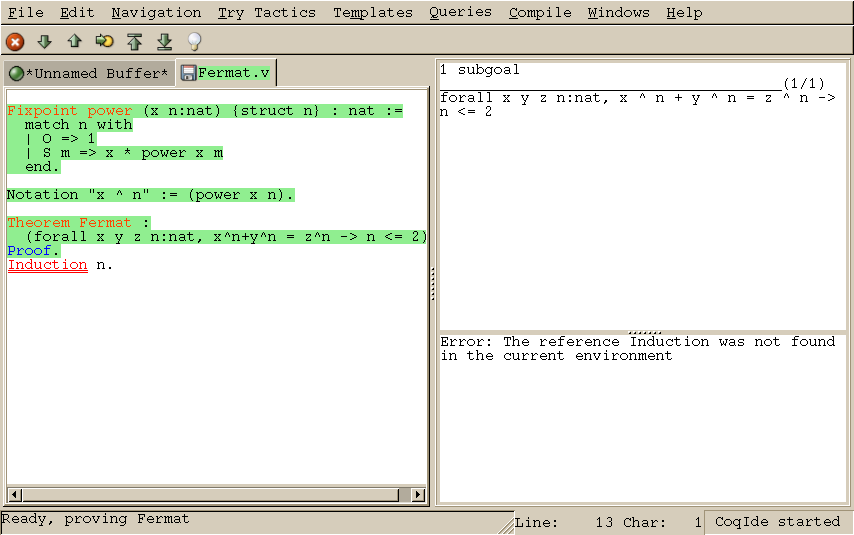
\includegraphics[width=1.0\textwidth]{coqide.png}
\else
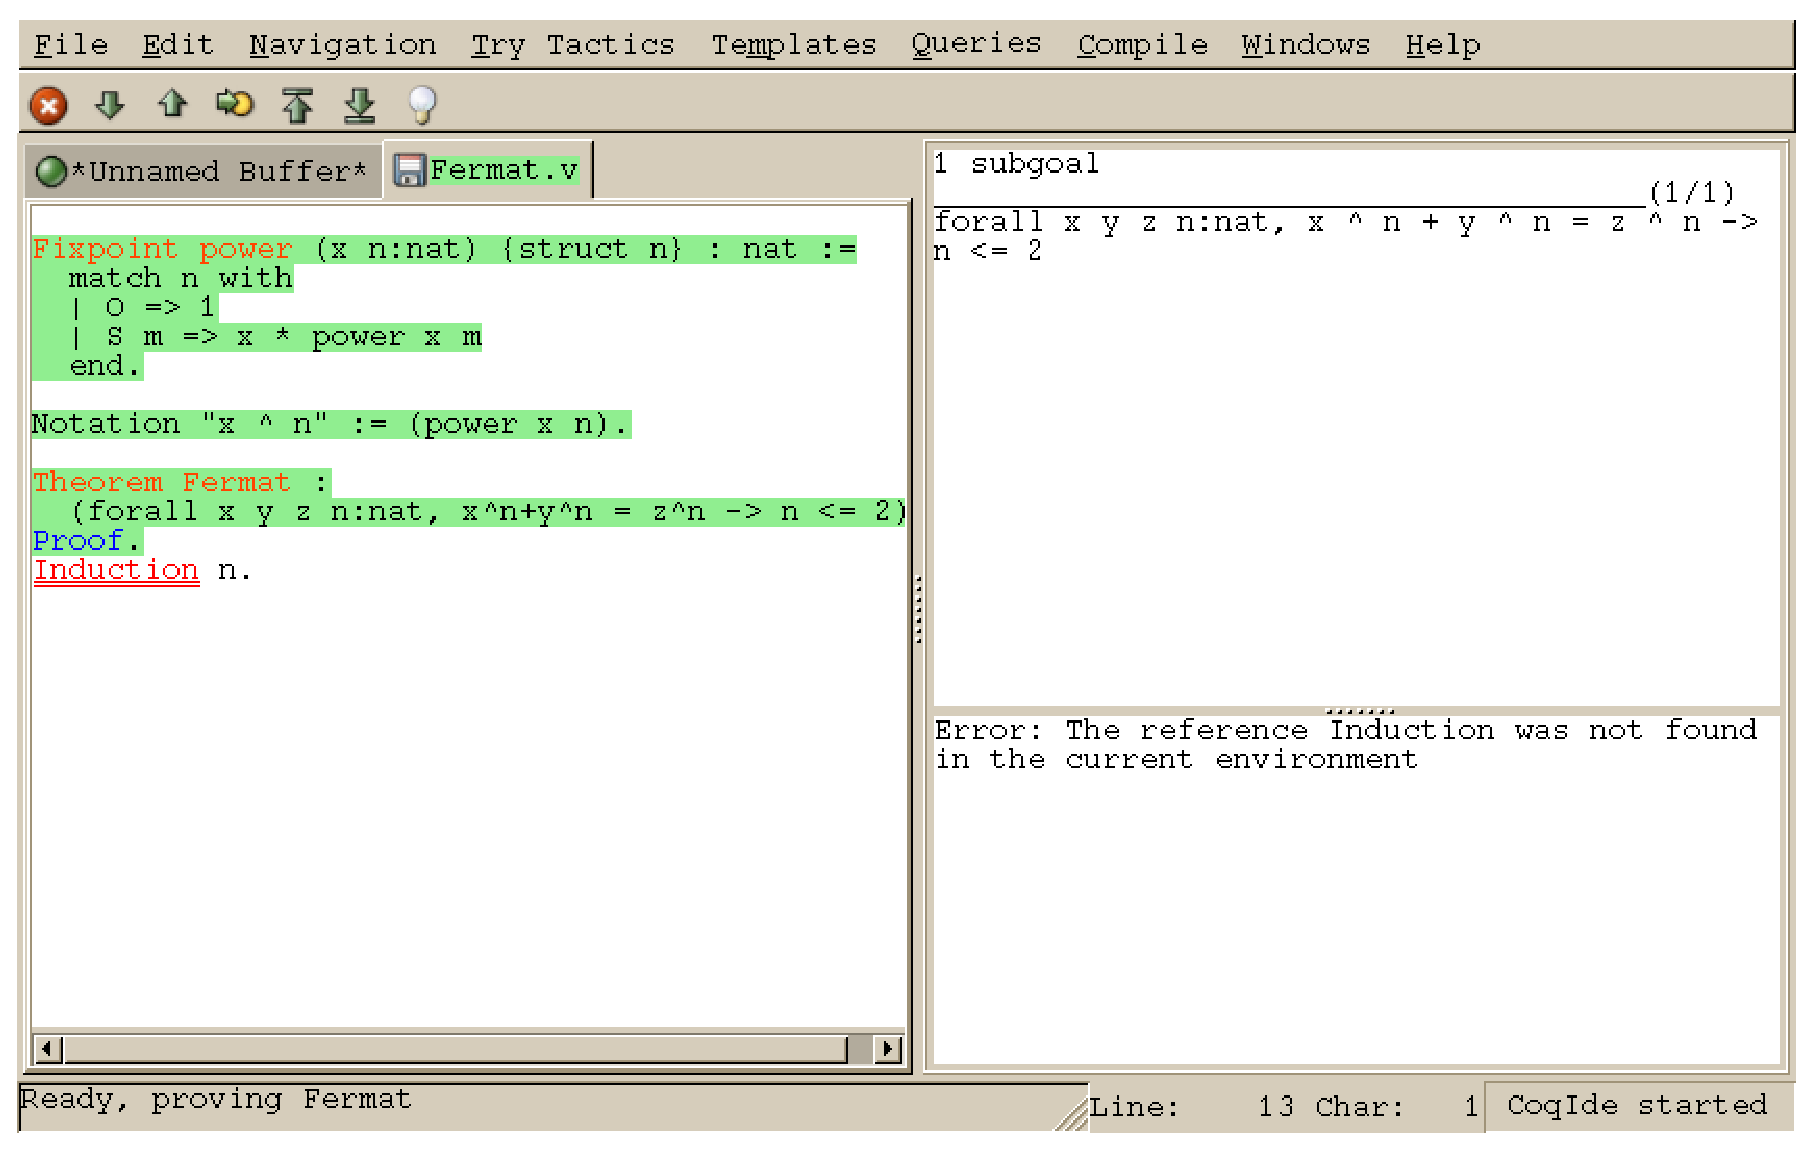
\includegraphics[width=1.0\textwidth]{coqide.eps}
\fi
%END LATEX
\end{center}
\caption{\CoqIDE{} main screen}
\label{fig:coqide}
\end{figure}

A sample \CoqIDE{} main screen, while navigating into a file
\verb|Fermat.v|, is shown on Figure~\ref{fig:coqide}.  At
the top is a menu bar, and a tool bar below it. The large window on
the left is displaying the various \emph{script buffers}. The upper right
window is the \emph{goal window}, where goals to 
prove are displayed. The lower right window is the \emph{message window},
where various messages resulting from commands are displayed. At the
bottom is the status bar.

\section{Managing files and buffers, basic edition}

In the script window, you may open arbitrarily many buffers to
edit. The \emph{File} menu allows you to open files or create some,
save them, print or export them into various formats. Among all these
buffers, there is always one which is the current \emph{running
  buffer}, whose name is displayed on a green background, which is the
one where Coq commands are currently executed. 

Buffers may be edited as in any text editor, and classical basic
editing commands (Copy/Paste, \ldots) are available in the \emph{Edit}
menu. \CoqIDE{} offers only basic editing commands, so if you need
more complex editing commands, you may launch your favorite text
editor on the current buffer, using the \emph{Edit/External Editor}
menu. 

\section{Interactive navigation into \Coq{} scripts}

The running buffer is the one where navigation takes place. The
toolbar proposes five basic commands for this. The first one,
represented by a down arrow icon, is for going forward executing one
command. If that command is successful, the part of the script that
has been executed is displayed on a green background. If that command
fails, the error message is displayed in the message window, and the
location of the error is emphasized by a red underline.

On Figure~\ref{fig:coqide}, the running buffer is \verb|Fermat.v|, all
commands until the \verb|Theorem| have been already executed, and the
user tried to go forward executing \verb|Induction n|. That command
failed because no such tactic exist (tactics are now in
lowercase\ldots), and the wrong word is underlined. 

Notice that the green part of the running buffer is not editable. If
you ever want to modify something you have to go backward using the up
arrow tool, or even better, put the cursor where you want to go back
and use the \textsf{goto} button. Unlike with \verb|coqtop|, you
should never use \verb|Undo| to go backward.

Two additional tool buttons exist, one to go directly to the end and
one to go back to the beginning. If you try to go to the end, or in
general to run several commands using the \textsf{goto} button, the
  execution will stop whenever an error is found.

If you ever try to execute a command which happens to run during a
long time, and would like to abort it before its
termination, you may use the interrupt button (the white cross on a red circle).
 
Finally, notice that these navigation buttons are also available in
the menu, where their keyboard shortcuts are given.

\section{Try tactics automatically}
\label{sec:trytactics}

The menu \texttt{Try Tactics} provides some features for automatically
trying to solve the current goal using simple tactics. If such a
tactic succeeds in solving the goal, then its text is automatically
inserted into the script. There is finally a combination of these
tactics, called the \emph{proof wizard} which will try each of them in
turn. This wizard is also available as a tool button (the light
bulb).  The set of tactics tried by the wizard is customizable in
the preferences.

These tactics are general ones, in particular they do not refer to
particular hypotheses. You may also try specific tactics related to
the goal or one of the hypotheses, by clicking with the right mouse
button one the goal or the considered hypothesis. This is the
``contextual menu on goals'' feature, that may be disabled in the
preferences if undesirable.
 
\section{Vernacular commands, templates}

The \texttt{Templates} menu allows to use shortcuts to insert
vernacular commands. This is a nice way to proceed if you are not sure
of the spelling of the command you want.

Moreover, this menu offers some \emph{templates} which will automatic
insert a complex command like Fixpoint with a convenient shape for its
arguments. 

\section{Queries}

\begin{figure}[t]
\begin{center}
%HEVEA\imgsrc{coqide-queries.png}
%BEGIN LATEX
\ifpdf  % si on est en pdflatex
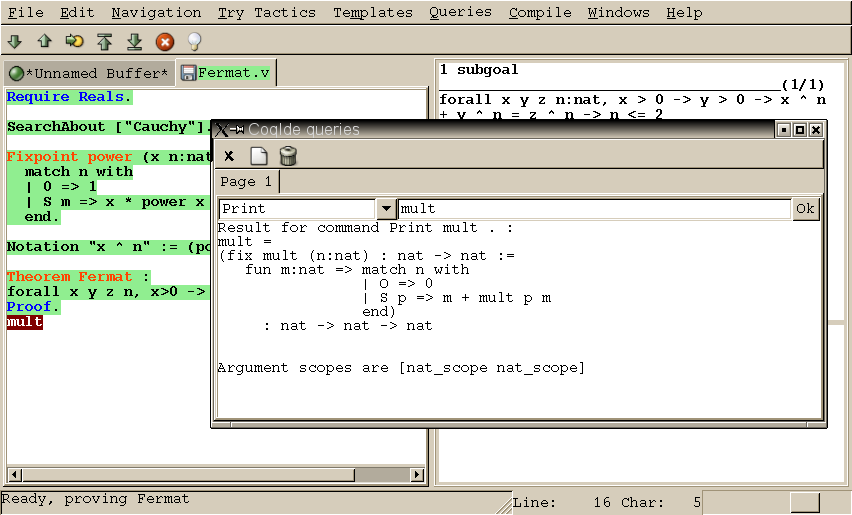
\includegraphics[width=1.0\textwidth]{coqide-queries.png}
\else
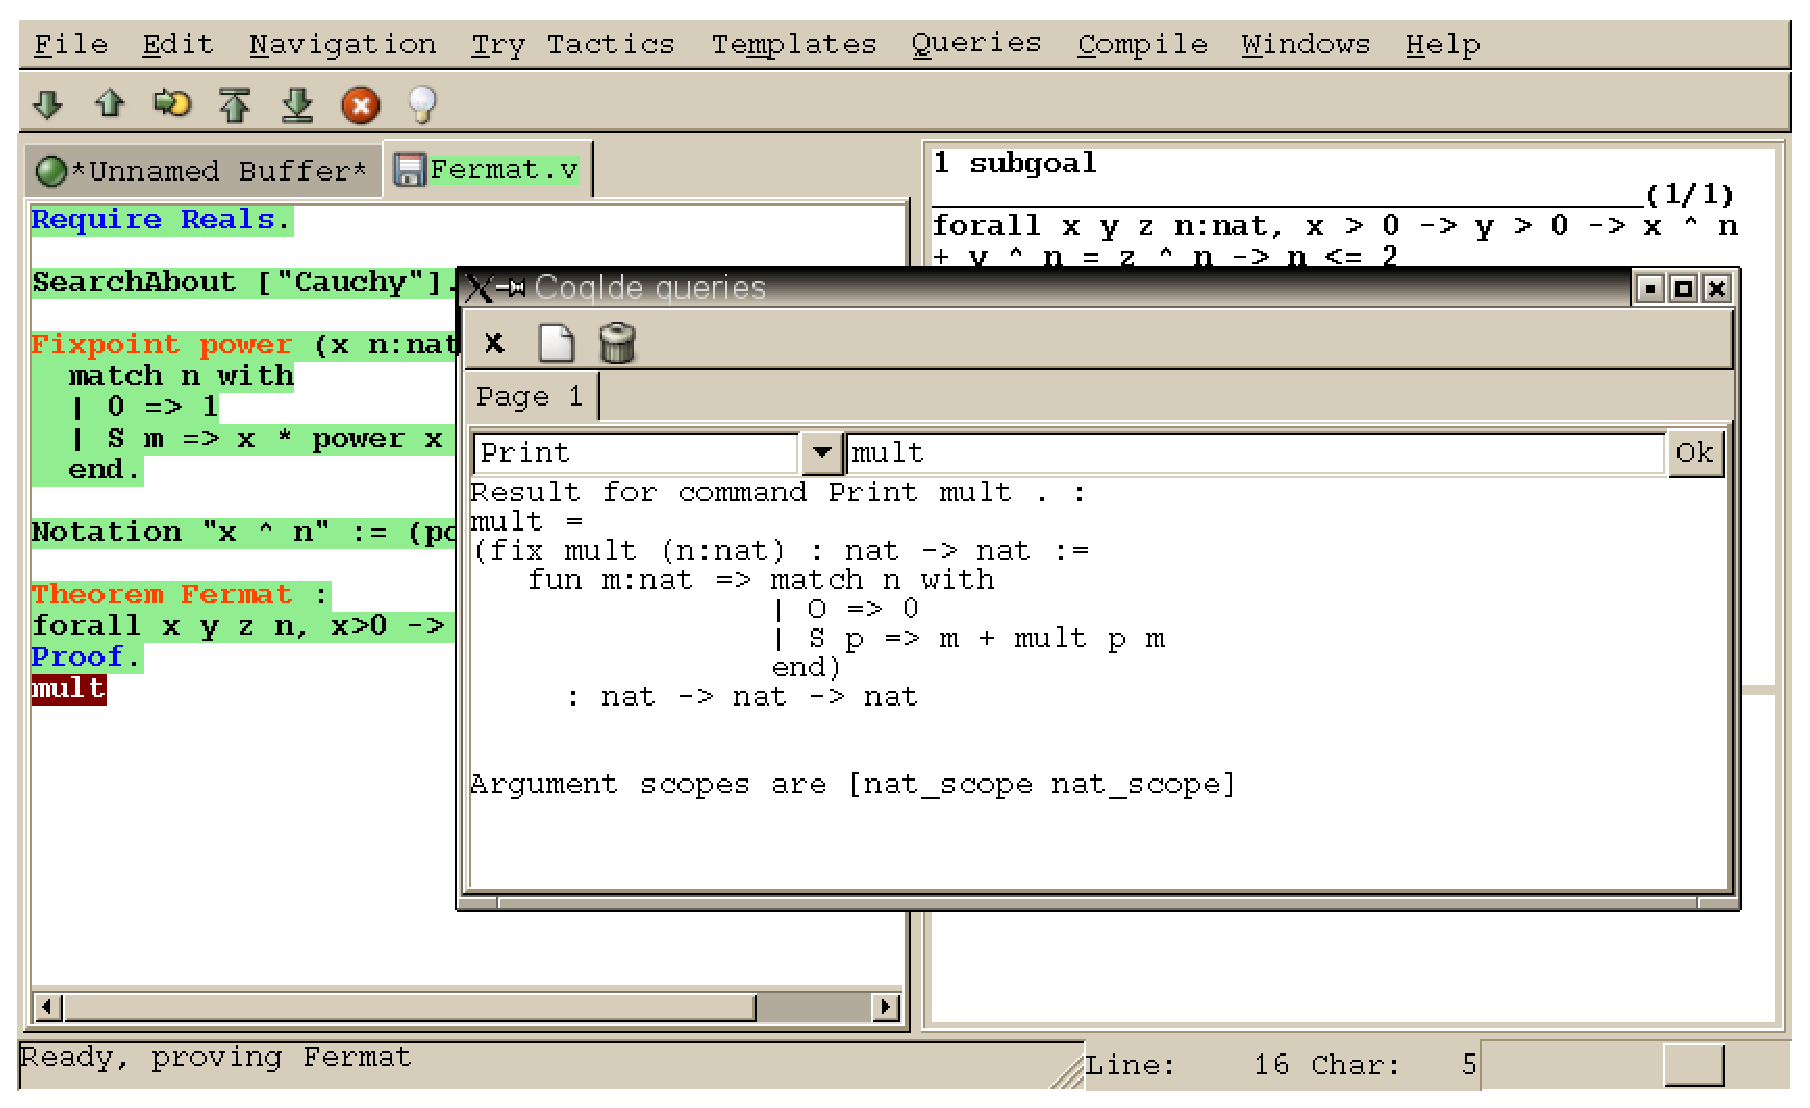
\includegraphics[width=1.0\textwidth]{coqide-queries.eps}
\fi
%END LATEX
\end{center}
\caption{\CoqIDE{}: the query window}
\label{fig:querywindow}
\end{figure}


We call \emph{query} any vernacular command that do not change the
current state, such as \verb|Check|, \verb|SearchAbout|, etc. Those
commands are of course useless during compilation of a file, hence
should not be included in scripts. To run such commands without
writing them in the script, \CoqIDE{} offers another input window
called the \emph{query window}. This window can be displayed on
demand, either by using the \texttt{Window} menu, or directly using
shortcuts given in the \texttt{Queries} menu. Indeed, with \CoqIDE{}
the simplest way to perform a \texttt{SearchAbout} on some identifier
is to select it using the mouse, and pressing \verb|F2|. This will
both make appear the query window and run the \texttt{SearchAbout} in
it, displaying the result. Shortcuts \verb|F3| and \verb|F4| are for
\verb|Check| and \verb|Print| respectively.
Figure~\ref{fig:querywindow} displays the query window after selection
of the word ``mult'' in the script windows, and pressing \verb|F4| to
print its definition.

\section{Compilation}

The \verb|Compile| menu offers direct commands to:
\begin{itemize}
\item compile the current buffer
\item run a compilation using \verb|make|
\item go to the last compilation error
\item create a \verb|makefile| using \verb|coq_makefile|.
\end{itemize}

\section{Customizations}

You may customize your environment using menu
\texttt{Edit/Preferences}. A new window will be displayed, with
several customization sections presented as a notebook. 

The first section is for selecting the text font used for scripts, goal
and message windows. 

The second section is devoted to file management: you may
configure automatic saving of files, by periodically saving the
contents into files named \verb|#f#| for each opened file
\verb|f|. You may also activate the \emph{revert} feature: in case a
opened file is modified on the disk by a third party, \CoqIDE{} may read
it again for you. Note that in the case you edited that same file, you
will be prompt to choose to either discard your changes or not. The
\texttt{File charset encoding} choice is described below in
Section~\ref{sec:coqidecharencoding}
 

The \verb|Externals| section allows to customize the external commands
for compilation, printing, web browsing. In the browser command, you
may use \verb|%s| to denote the URL to open, for example: %
\verb|mozilla -remote "OpenURL(%s)"|. 

The \verb|Tactics Wizard| section allows to defined the set of tactics
that should be tried, in sequence, to solve the current goal.

The last section is for miscellaneous boolean settings, such as the
``contextual menu on goals'' feature presented in
Section~\ref{sec:trytactics}. 

Notice that these settings are saved in the file \verb|.coqiderc| of
your home directory. 

A gtk2 accelerator keymap is saved under the name \verb|.coqide.keys|.
This file should not be edited manually: to modify a given menu
shortcut, go to the corresponding menu item without releasing the
mouse button, press the key you want for the new shortcut, and release
the mouse button afterwards.

For experts: it is also possible to set up a specific gtk resource
file, under the name \verb|.coqide-gtk2rc|, following the gtk2
resources syntax
\url{http://developer.gnome.org/doc/API/2.0/gtk/gtk-Resource-Files.html}.
Such a default resource file exists in the \Coq{} library, you may
copy this file into your home directory, and edit it using any text
editor, \CoqIDE{} itself for example.

\section{Using unicode symbols}

\CoqIDE{} supports unicode character encoding in its text windows,
consequently a large set of symbols is available for notations.

\subsection{Displaying unicode symbols}

You just need to define suitable notations as described in
Chapter~\ref{Addoc-syntax}. For example, to use the mathematical symbols
$\forall$ and $\exists$, you may define 
\begin{quote}\tt
Notation "$\forall$ x : t, P" := \\
\qquad  (forall x:t, P) (at level 200, x ident).\\
Notation "$\exists$ x : t, P" := \\
\qquad  (exists x:t, P) (at level 200, x ident).
\end{quote}
There exists a small set of such notations already defined, in the
file \verb|utf8.v| of \Coq{} library, so you may enable them just by 
\verb|Require utf8| inside \CoqIDE{}, or equivalently, by starting
\CoqIDE{} with \verb|coqide -l utf8|.

However, there are some issues when using such unicode symbols: you of
course need to use a character font which supports them. In the Fonts
section of the preferences, the Preview line displays some unicode symbols, so
you could figure out if the selected font is OK. Related to this, one
thing you may need to do is choose whether Gtk should use antialiased
fonts or not, by setting the environment variable \verb|GDK_USE_XFT|
to 1 or 0 respectively.

\subsection{Defining an input method for non ASCII symbols}

To input an Unicode symbol, a general method is to press both the
CONTROL and the SHIFT keys, and type the hexadecimal code of the
symbol required, for example \verb|2200| for the $\forall$ symbol.
A list of symbol codes is available at \url{http://www.unicode.org}. 

Of course, this method is painful for symbols you use often. There is
always the possibility to copy-paste a symbol already typed in.
Another method is to bind some key combinations for frequently used
symbols. For example, to bind keys \verb|F11| and \verb|F12| to
$\forall$ and $\exists$ respectively, you may add
\begin{quote}\tt
  bind "F11" {"insert-at-cursor" ("$\forall$")}\\
  bind "F12" {"insert-at-cursor" ("$\exists$")}
\end{quote}
to your \verb|binding "text"| section in \verb|.coqiderc-gtk2rc|.


%  such a binding is system-dependent. We
% give here a solution for X11:
% \begin{itemize}
% \item first, using \verb|xmodmap|, bind some key combination into a
%   new key name such as Fxx where xx greater that 12: for example (on a
%   french keyboard)
%   \begin{quote}\tt
%     xmodmap -e "keycode  24 = a A F13 F13" \\
%     xmodmap -e "keycode  26 = e E F14 F14" 
%   \end{quote}
%   will rebind "<AltGr>a" to F13 and "<AltGr>e" to F14.
% \item then add   
%   \begin{quote}\tt
%     bind "F13" {"insert-at-cursor" ("$\forall$")}\\
%     bind "F14" {"insert-at-cursor" ("$\exists$")}
%   \end{quote}
%   to your \verb|binding "text"| section in \verb|.coqiderc-gtk2rc|.
%        The strange \verb|∀| argument is the UTF-8 encoding for
%        0x2200, that is the symbol $\forall$. Computing UTF-8 encoding
%        for a unicode can be done in various ways, including
%        launching a \verb|lablgtk2| toplevel and use
%\begin{verbatim}
%     Glib.Utf8.from_unichar 0x2200;;
%\end{verbatim}
%\end{itemize}

\subsection{Character encoding for saved files}
\label{sec:coqidecharencoding}

In the \texttt{Files} section of the preferences, the encoding option
is related to the way files are saved. 

If you have no need to exchange files with non UTF-8 aware
applications, it is better to choose the UTF-8 encoding, since it
guarantees that your files will be read again without problems. (This
is because when \CoqIDE{} reads a file, it tries to automatically
detect its character encoding.) 

If you choose something else than UTF-8, then missing characters will
be written encoded by \verb|\x{....}| or \verb|\x{........}| where
each dot is an hexadecimal digit: the number between braces is the
hexadecimal UNICODE index for the missing character.


\section{Building a custom \CoqIDE{} with user \textsc{ML} code}

You can do this as described in Section~\ref{Coqmktop} for a
custom coq text toplevel, simply by adding 
option \verb|-ide| to \verb|coqmktop|, that is something like
\begin{quote}
\texttt{coqmktop -ide -byte $m_1$.cmo \ldots{} $m_n$.cmo}
\end{quote}
or 
\begin{quote}
\texttt{coqmktop -ide -opt $m_1$.cmx \ldots{} $m_n$.cmx}
\end{quote}

    

% $Id: RefMan-ide.tex 8626 2006-03-14 15:01:00Z notin $ 

%%% Local Variables: 
%%% mode: latex
%%% TeX-master: "Reference-Manual"
%%% End: 
% Coq IDE

%BEGIN LATEX
\RefManCutCommand{BEGINADDENDUM=\thepage}
%END LATEX
\part{Addendum to the Reference Manual}
%\coverpage{Addendum to the Reference Manual}{\ }
%\addcontentsline{toc}{part}{Additional documentation}
\setheaders{Presentation of the Addendum}
\chapter*{Presentation of the Addendum}

Here you will find several pieces of additional documentation for the
\Coq\ Reference Manual. Each of this chapters is concentrated on a
particular topic, that should interest only a fraction of the \Coq\
users: that's the reason why they are apart from the Reference
Manual.

\begin{description}

\item[Extended pattern-matching] This chapter details the use of
  generalized pattern-matching. It is contributed by Cristina Cornes
  and Hugo Herbelin.

\item[Implicit coercions] This chapter details the use of the coercion
  mechanism.  It is contributed by Amokrane Sa�bi.

%\item[Proof of imperative programs] This chapter explains how to
%  prove properties of annotated programs with imperative features.
%  It is contributed by Jean-Christophe Filli�tre

\item[Program extraction] This chapter explains how to extract in practice ML
  files from $\FW$ terms.   It is contributed by Jean-Christophe
  Filli�tre and Pierre Letouzey.

%\item[Natural] This chapter is due to Yann Coscoy. It is the user
%  manual of the tools he wrote for printing proofs in natural
%  language. At this time, French and English languages are supported.

\item[omega] \texttt{omega}, written by Pierre Cr�gut, solves a whole
  class of arithmetic problems.

%\item[Program] The \texttt{Program} technology intends to inverse the
%  extraction mechanism. It allows the developments of certified
%  programs in \Coq. This chapter is due to Catherine Parent. {\bf This
%  feature is not available in {\Coq} version 7.}

\item[The {\tt ring} tactic] This is a tactic to do AC rewriting. This
  chapter explains how to use it and how it works.
  The chapter is contributed by Patrick Loiseleur.

\item[The {\tt Setoid\_replace} tactic] This is a
  tactic to do rewriting on types equipped with specific (only partially
  substitutive) equality. The chapter is contributed by Cl�ment Renard.


\end{description}

\atableofcontents


%%% Local Variables: 
%%% mode: latex
%%% TeX-master: "Reference-Manual"
%%% End: 
%
\achapter{Extended pattern-matching}\defaultheaders
\aauthor{Cristina Cornes and Hugo Herbelin}

\label{Mult-match-full}
\ttindex{Cases}
\index{ML-like patterns}

This section describes the full form of pattern-matching in {\Coq} terms.

\asection{Patterns}\label{implementation} The full syntax of {\tt
match} is presented in figures~\ref{term-syntax}
and~\ref{term-syntax-aux}.  Identifiers in patterns are either
constructor names or variables. Any identifier that is not the
constructor of an inductive or coinductive type is considered to be a
variable. A variable name cannot occur more than once in a given
pattern. It is recommended to start variable names by a lowercase
letter.

If a pattern has the form $(c~\vec{x})$ where $c$ is a constructor
symbol and $\vec{x}$ is a linear vector of (distinct) variables, it is
called {\em simple}: it is the kind of pattern recognized by the basic
version of {\tt match}. On the opposite, if it is a variable $x$ or
has the form $(c~\vec{p})$ with $p$ not only made of variables, the
pattern is called {\em nested}.

A variable pattern matches any value, and the identifier is bound to
that value. The pattern ``\texttt{\_}'' (called ``don't care'' or
``wildcard'' symbol) also matches any value, but does not bind
anything. It may occur an arbitrary number of times in a
pattern. Alias patterns written \texttt{(}{\sl pattern} \texttt{as}
{\sl identifier}\texttt{)} are also accepted. This pattern matches the
same values as {\sl pattern} does and {\sl identifier} is bound to the
matched value.  
A pattern of the form {\pattern}{\tt |}{\pattern} is called
disjunctive. A list of patterns separated with commas is also
considered as a pattern and is called {\em multiple pattern}. However
multiple patterns can only occur at the root of pattern-matching
equations. Disjunctions of {\em multiple pattern} are allowed though.

Since extended {\tt match} expressions are compiled into the primitive
ones, the expressiveness of the theory remains the same. Once the
stage of parsing has finished only simple patterns remain.  Re-nesting
of pattern is performed at printing time. An easy way to see the
result of the expansion is to toggle off the nesting performed at
printing (use here {\tt Set Printing Matching}), then by printing the term
with \texttt{Print} if the term is a constant, or using the command
\texttt{Check}.

The extended \texttt{match} still accepts an optional {\em elimination
predicate} given after the keyword \texttt{return}.  Given a pattern
matching expression, if all the right-hand-sides of \texttt{=>} ({\em
rhs} in short) have the same type, then this type can be sometimes
synthesized, and so we can omit the \texttt{return} part. Otherwise 
the predicate after \texttt{return} has to be provided, like for the basic
\texttt{match}.

Let us illustrate through examples the different aspects of extended
pattern matching. Consider for example the function that computes the
maximum of two natural numbers. We can write it in primitive syntax
by:

\begin{coq_example}
Fixpoint max (n m:nat) {struct m} : nat :=
  match n with
  | O => m
  | S n' => match m with
            | O => S n'
            | S m' => S (max n' m')
            end
  end.
\end{coq_example}

\paragraph{Multiple patterns}

Using multiple patterns in the definition of {\tt max} allows to write:

\begin{coq_example}
Reset max.
Fixpoint max (n m:nat) {struct m} : nat :=
  match n, m with
  | O, _ => m
  | S n', O => S n'
  | S n', S m' => S (max n' m')
  end.
\end{coq_example}

which will be compiled into the previous form.

The pattern-matching compilation strategy examines patterns from left
to right. A \texttt{match} expression is generated {\bf only} when
there is at least one constructor in the column of patterns. E.g. the
following example does not build a \texttt{match} expression.

\begin{coq_example}
Check (fun x:nat => match x return nat with
                    | y => y
                    end).
\end{coq_example}

\paragraph{Aliasing subpatterns}

We can also use ``\texttt{as} {\ident}'' to associate a name to a
sub-pattern:

\begin{coq_example}
Reset max.
Fixpoint max (n m:nat) {struct n} : nat :=
  match n, m with
  | O, _ => m
  | S n' as p, O => p
  | S n', S m' => S (max n' m')
  end.
\end{coq_example}

\paragraph{Nested patterns}

Here is now an example of nested patterns:

\begin{coq_example}
Fixpoint even (n:nat) : bool :=
  match n with
  | O => true
  | S O => false
  | S (S n') => even n'
  end.
\end{coq_example}

This is compiled into:

\begin{coq_example}
Print even.
\end{coq_example}

In the previous examples patterns do not conflict with, but
sometimes it is comfortable to write patterns that admit a non
trivial superposition. Consider
the boolean function \texttt{lef} that given two natural numbers
yields \texttt{true} if the first one is less or equal than the second
one and \texttt{false} otherwise. We can write it as follows:

\begin{coq_example}
Fixpoint lef (n m:nat) {struct m} : bool :=
  match n, m with
  | O, x => true
  | x, O => false
  | S n, S m => lef n m
  end.
\end{coq_example}

Note that the first and the second multiple pattern superpose because
the couple of values \texttt{O O} matches both. Thus, what is the result
of the function on those values?  To eliminate ambiguity we use the
{\em textual priority rule}: we consider patterns ordered from top to
bottom, then a value is matched by the pattern at the $ith$ row if and
only if it is not matched by some pattern of a previous row. Thus in the
example,
\texttt{O O} is matched by the first pattern, and so \texttt{(lef O O)}
yields \texttt{true}.

Another way to write  this function is:

\begin{coq_example}
Reset lef.
Fixpoint lef (n m:nat) {struct m} : bool :=
  match n, m with
  | O, x => true
  | S n, S m => lef n m
  | _, _ => false
  end.
\end{coq_example}

Here the last pattern superposes with the first two. Because
of the priority rule, the last pattern 
will be used only for values that do not match neither the  first nor
the second one.  

Terms with useless patterns are not accepted by the
system. Here is an example:
% Test failure
\begin{coq_eval}
Set Printing Depth 50.
  (********** The following is not correct and should produce **********)
  (**************** Error: This clause is redundant ********************)
\end{coq_eval}
\begin{coq_example}
Check (fun x:nat =>
         match x with
         | O => true
         | S _ => false
         | x => true
         end).
\end{coq_example}

\paragraph{Disjunctive patterns}

Multiple patterns that share the same right-hand-side can be
factorized using the notation \nelist{\multpattern}{\tt |}. For instance,
{\tt max} can be rewritten as follows:

\begin{coq_eval}
Reset max.
\end{coq_eval}
\begin{coq_example}
Fixpoint max (n m:nat) {struct m} : nat :=
  match n, m with
  | S n', S m' => S (max n' m')
  | 0, p | p, 0 => p
  end.
\end{coq_example}

Similarly, factorization of (non necessary multiple) patterns
that share the same variables is possible by using the notation
\nelist{\pattern}{\tt |}. Here is an example:

\begin{coq_example}
Definition filter_2_4 (n:nat) : nat :=
  match n with
  | 2 as m | 4 as m => m
  | _ => 0
  end.
\end{coq_example}

Here is another example using disjunctive subpatterns.

\begin{coq_example}
Definition filter_some_square_corners (p:nat*nat) : nat*nat :=
  match p with
  | ((2 as m | 4 as m), (3 as n | 5 as n)) => (m,n)
  | _ => (0,0)
  end.
\end{coq_example}

\asection{About patterns of parametric types}
When matching objects of a parametric type, constructors in patterns
{\em do not expect} the parameter arguments. Their value is deduced
during expansion.
Consider for example the type of polymorphic lists:

\begin{coq_example}
Inductive List (A:Set) : Set :=
  | nil : List A
  | cons : A -> List A -> List A.
\end{coq_example}

We can check the function {\em tail}:

\begin{coq_example}
Check
  (fun l:List nat =>
     match l with
     | nil => nil nat
     | cons _ l' => l'
     end).
\end{coq_example}


When we use parameters in patterns there is an error message:
% Test failure
\begin{coq_eval}
Set Printing Depth 50.
(********** The following is not correct and should produce **********)
(******** Error: The constructor cons expects 2 arguments ************)
\end{coq_eval}
\begin{coq_example}
Check
  (fun l:List nat =>
     match l with
     | nil A => nil nat
     | cons A _ l' => l'
     end).
\end{coq_example}



\asection{Matching objects of dependent types}
The previous examples illustrate pattern matching on objects of
non-dependent types, but we can also 
use the expansion strategy to destructure objects of dependent type.
Consider the type \texttt{listn} of lists of a certain length:

\begin{coq_example}
Inductive listn : nat -> Set :=
  | niln : listn 0
  | consn : forall n:nat, nat -> listn n -> listn (S n).
\end{coq_example}

\asubsection{Understanding dependencies in patterns}
We can define the function \texttt{length} over \texttt{listn} by:

\begin{coq_example}
Definition length (n:nat) (l:listn n) := n.
\end{coq_example}

Just for illustrating pattern matching, 
we can define it by case analysis:

\begin{coq_example}
Reset length.
Definition length (n:nat) (l:listn n) :=
  match l with
  | niln => 0
  | consn n _ _ => S n
  end.
\end{coq_example}

We can understand the meaning of this definition using the
same notions of usual pattern matching.

%
% Constraining of dependencies is not longer valid in V7
%
\iffalse
Now suppose we split the second pattern  of \texttt{length} into two 
cases so to give an
alternative definition using nested patterns:
\begin{coq_example}
Definition length1 (n:nat) (l:listn n) :=
  match l with
  | niln => 0
  | consn n _ niln => S n
  | consn n _ (consn _ _ _) => S n
  end.
\end{coq_example}

It is obvious that \texttt{length1} is  another version of
\texttt{length}. We can also give the following definition:
\begin{coq_example}
Definition length2 (n:nat) (l:listn n) :=
  match l with
  | niln => 0
  | consn n _ niln => 1
  | consn n _ (consn m _ _) => S (S m)
  end.
\end{coq_example}

If we forget that \texttt{listn} is a dependent type and we read these
definitions using the usual semantics of pattern matching,  we can conclude
that \texttt{length1}
and \texttt{length2} are different functions.
In fact, they are equivalent
because the pattern \texttt{niln} implies that \texttt{n} can only match
the value $0$ and analogously the pattern \texttt{consn} determines that \texttt{n} can
only match  values of the form  $(S~v)$ where $v$ is the value matched by
\texttt{m}. 

The converse is also true. If
we destructure the  length  value with the pattern \texttt{O} then the list
value should be $niln$. 
Thus, the following term \texttt{length3} corresponds to the function
\texttt{length} but this time defined by case analysis on the dependencies instead of on the list:

\begin{coq_example}
Definition length3 (n:nat) (l:listn n) :=
  match l with
  | niln => 0
  | consn O _ _ => 1
  | consn (S n) _ _ => S (S n)
  end.
\end{coq_example}

When we have nested patterns of dependent types, the semantics of
pattern matching becomes a little more difficult because
the set of values that are matched by a sub-pattern may be conditioned by the
values matched by another sub-pattern. Dependent nested patterns are
somehow constrained patterns. 
In the examples, the expansion of
\texttt{length1} and \texttt{length2} yields exactly the same term
 but the
expansion of \texttt{length3} is completely different. \texttt{length1} and
\texttt{length2} are expanded into two nested case analysis on
\texttt{listn} while \texttt{length3} is expanded into a case analysis on
\texttt{listn} containing a case analysis on natural numbers inside.


In practice the user can think about the patterns as independent and
it is the expansion algorithm that cares to relate them. \\
\fi
%
%
%

\asubsection{When the elimination predicate must be provided}
The examples  given so far do not need an explicit elimination predicate
 because all the rhs have the same type and the
strategy succeeds to synthesize it.
Unfortunately when dealing with dependent patterns it often happens
that we need to write cases where the type of the rhs are 
different  instances of the elimination  predicate.
The function  \texttt{concat} for \texttt{listn}
is an example where the branches have different type
and we need to provide the elimination predicate:

\begin{coq_example}
Fixpoint concat (n:nat) (l:listn n) (m:nat) (l':listn m) {struct l} :
 listn (n + m) :=
  match l in listn n return listn (n + m) with
  | niln => l'
  | consn n' a y => consn (n' + m) a (concat n' y m l')
  end.
\end{coq_example}
The elimination predicate is {\tt fun (n:nat) (l:listn n) => listn~(n+m)}.
In general if $m$ has type $(I~q_1\ldots q_r~t_1\ldots t_s)$ where 
$q_1\ldots q_r$ are parameters, the elimination predicate should be of
the form~:
{\tt fun $y_1$\ldots $y_s$ $x$:($I$~$q_1$\ldots $q_r$~$y_1$\ldots
  $y_s$) => P}. 

In the concrete syntax, it should be written~:
\[ \kw{match}~m~\kw{as}~x~\kw{in}~(I~\_\ldots \_~y_1\ldots y_s)~\kw{return}~Q~\kw{with}~\ldots~\kw{end}\]

The variables which appear in the \kw{in} and \kw{as} clause are new
and bounded in the property $Q$ in the \kw{return} clause. The
parameters of the inductive definitions should not be mentioned and
are replaced by \kw{\_}.

Recall that a list of patterns is also a pattern. So, when
we destructure several terms at the same time and the branches have
different type  we need to provide
the elimination predicate for this multiple pattern. 
It is done using the same scheme, each term may be associated to an
\kw{as} and \kw{in} clause in order to introduce a dependent product.

For example, an equivalent definition for \texttt{concat} (even though the matching on the second term is trivial) would have
been:

\begin{coq_example}
Reset concat.
Fixpoint concat (n:nat) (l:listn n) (m:nat) (l':listn m) {struct l} :
 listn (n + m) :=
  match l in listn n, l' return listn (n + m) with
  | niln, x => x
  | consn n' a y, x => consn (n' + m) a (concat n' y m x)
  end.
\end{coq_example}

% Notice that this time, the predicate \texttt{[n,\_:nat](listn (plus n
%   m))}  is binary because we
% destructure both \texttt{l} and \texttt{l'} whose types have arity one.
% In general, if we destructure the terms $e_1\ldots e_n$
% the predicate will be of arity $m$ where $m$ is the sum of the
% number of dependencies of the type of $e_1, e_2,\ldots e_n$ 
% (the $\lambda$-abstractions
% should correspond from left to right to each dependent argument of the
% type of $e_1\ldots e_n$).
When the arity of the predicate (i.e. number of abstractions) is not
correct Coq raises an error message. For example:

% Test failure
\begin{coq_eval}
Reset concat.
Set Printing Depth 50.
(********** The following is not correct and should produce ***********)
(** Error: the term l' has type listn m while it is expected to have **)
(** type listn (?31 + ?32)                                           **)
\end{coq_eval}
\begin{coq_example}
Fixpoint concat
 (n:nat) (l:listn n) (m:nat)
 (l':listn m) {struct l} : listn (n + m) :=
  match l, l' with
  | niln, x => x
  | consn n' a y, x => consn (n' + m) a (concat n' y m x)
  end.
\end{coq_example}

\asection{Using pattern matching to write proofs}
In all the previous examples the elimination predicate does not depend
on the object(s) matched. But it may depend and the typical case 
is when we write a proof by induction or a function that yields an
object of dependent type. An example of proof using \texttt{match} in
given in section \ref{refine-example}

For example, we can write 
the function \texttt{buildlist} that given a natural number
$n$ builds a list of length $n$ containing zeros as follows:

\begin{coq_example}
Fixpoint buildlist (n:nat) : listn n :=
  match n return listn n with
  | O => niln
  | S n => consn n 0 (buildlist n)
  end.
\end{coq_example}

We can also use multiple patterns. 
Consider the following definition of the predicate less-equal
\texttt{Le}:

\begin{coq_example}
Inductive LE : nat -> nat -> Prop :=
  | LEO : forall n:nat, LE 0 n
  | LES : forall n m:nat, LE n m -> LE (S n) (S m).
\end{coq_example}

We can use multiple patterns to write  the proof of the lemma
 \texttt{forall (n m:nat), (LE n m)}\verb=\/=\texttt{(LE m n)}:

\begin{coq_example}
Fixpoint dec (n m:nat) {struct n} : LE n m \/ LE m n :=
  match n, m return LE n m \/ LE m n with
  | O, x => or_introl (LE x 0) (LEO x)
  | x, O => or_intror (LE x 0) (LEO x)
  | S n as n', S m as m' =>
      match dec n m with
      | or_introl h => or_introl (LE m' n') (LES n m h)
      | or_intror h => or_intror (LE n' m') (LES m n h)
      end
  end.
\end{coq_example}
In the example of \texttt{dec},
the first \texttt{match} is dependent while 
the second is not.

% In general, consider the terms $e_1\ldots e_n$,
% where  the type of $e_i$ is an instance of a family type
% $\lb (\vec{d_i}:\vec{D_i}) \mto T_i$  ($1\leq i
% \leq n$). Then, in expression \texttt{match}  $e_1,\ldots,
% e_n$ \texttt{of} \ldots \texttt{end}, the 
% elimination predicate ${\cal P}$ should be of the form:
% $[\vec{d_1}:\vec{D_1}][x_1:T_1]\ldots [\vec{d_n}:\vec{D_n}][x_n:T_n]Q.$

The user can also use \texttt{match} in combination with the tactic
\texttt{refine} (see section \ref{refine}) to build incomplete proofs
beginning with a \texttt{match} construction.

\asection{Pattern-matching on inductive objects involving local
definitions}

If local definitions occur in the type of a constructor, then there
are two ways to match on this constructor. Either the local
definitions are skipped and matching is done only on the true arguments
of the constructors, or the bindings for local definitions can also
be caught in the matching.

Example.

\begin{coq_eval}
Reset Initial.
Require Import Arith.
\end{coq_eval}

\begin{coq_example*}
Inductive list : nat -> Set :=
  | nil : list 0
  | cons : forall n:nat, let m := (2 * n) in list m -> list (S (S m)).
\end{coq_example*}

In the next example, the local definition is not caught.

\begin{coq_example}
Fixpoint length n (l:list n) {struct l} : nat :=
  match l with
  | nil => 0
  | cons n l0 => S (length (2 * n) l0)
  end.
\end{coq_example}

But in this example, it is.

\begin{coq_example}
Fixpoint length' n (l:list n) {struct l} : nat :=
  match l with
  | nil => 0
  | cons _ m l0 => S (length' m l0)
  end.
\end{coq_example}

\Rem for a given matching clause, either none of the local
definitions or all of them can be caught.

\asection{Pattern-matching and coercions}

If a mismatch occurs between the expected type of a pattern and its
actual type, a coercion made from constructors is sought. If such a
coercion can be found, it is automatically inserted around the
pattern.

Example:

\begin{coq_example}
Inductive I : Set :=
  | C1 : nat -> I
  | C2 : I -> I.
Coercion C1 : nat >-> I.
Check (fun x => match x with
                | C2 O => 0
                | _ => 0
                end).
\end{coq_example}


\asection{When does the expansion strategy fail ?}\label{limitations}
The strategy works very like in ML languages when treating
patterns of non-dependent type.  
But there are new cases of failure that are due to the presence of 
dependencies. 

The error messages of the current implementation may be sometimes
confusing.  When the tactic fails because patterns are somehow
incorrect then error messages refer to the initial expression. But the
strategy may succeed to build an expression whose sub-expressions are
well typed when the whole expression is not. In this situation the
message makes reference to the expanded expression.  We encourage
users, when they have patterns with the same outer constructor in
different equations, to name the variable patterns in the same
positions with the same name.  
E.g. to write {\small\texttt{(cons n O x) => e1}} 
and {\small\texttt{(cons n \_ x) => e2}} instead of
{\small\texttt{(cons n O x) => e1}} and 
{\small\texttt{(cons n' \_ x') => e2}}. 
This helps to maintain certain name correspondence between the
generated expression and the original.

Here is a summary of the error messages corresponding to each situation:

\begin{ErrMsgs}
\item \sverb{The constructor } {\sl
    ident} \sverb{expects } {\sl num} \sverb{arguments}
  
 \sverb{The variable } {\sl ident} \sverb{is bound several times
    in pattern } {\sl term}
  
 \sverb{Found a constructor of inductive type} {\term}
 \sverb{while a constructor of} {\term} \sverb{is expected}

 Patterns are incorrect (because constructors are not applied to
  the correct number of the arguments, because they are not linear or
  they are wrongly typed)

\item \errindex{Non exhaustive pattern-matching}

the pattern matching is not exhaustive

\item \sverb{The elimination predicate } {\sl term} \sverb{should be
    of arity } {\sl num} \sverb{(for non dependent case) or } {\sl
    num} \sverb{(for dependent case)}

The elimination predicate provided to \texttt{match} has not the
  expected arity


%\item the whole expression is wrongly typed

% CADUC ?
% , or the synthesis of
%   implicit arguments fails (for example to find the elimination
%   predicate or to resolve implicit arguments in the rhs).
 
%   There are {\em nested patterns of dependent type}, the elimination
%   predicate corresponds to non-dependent case and has the form
%   $[x_1:T_1]...[x_n:T_n]T$ and {\bf some} $x_i$ occurs {\bf free} in
%   $T$.  Then, the strategy may fail to find out a correct elimination
%   predicate during some step of compilation.  In this situation we
%   recommend the user to rewrite the nested dependent patterns into
%   several \texttt{match} with {\em simple patterns}.
  
\item {\tt Unable to infer a match predicate\\
    Either there is a type incompatiblity or the problem involves\\
    dependencies}
 
  There is a type mismatch between the different branches

  Then the user should provide an elimination predicate.

% Obsolete ?  
% \item because of nested patterns, it may happen that even though all
%   the rhs have the same type, the strategy needs dependent elimination
%   and so an elimination predicate must be provided. The system warns
%   about this situation, trying to compile anyway with the
%   non-dependent strategy. The risen message is:

% \begin{itemize}
% \item {\tt Warning: This pattern matching may need dependent
%     elimination to be compiled.  I will try, but if fails try again
%     giving dependent elimination predicate.}
% \end{itemize}


%%%%%%%%%%%%%%%%%%%%%%%%%%%%%%%%%%%%%%%%%%%%%%%%%%%%%%%%%%%%%%%%%%%%%%
% % LA PROPAGATION DES CONTRAINTES ARRIERE N'EST PAS FAITE DANS LA V7
% TODO
% \item there are {\em nested patterns of dependent type} and the
%   strategy builds a term that is well typed but recursive calls in fix
%   point are reported as illegal:
% \begin{itemize}
% \item {\tt Error: Recursive call applied to an illegal term ...}
% \end{itemize}

% This is because the strategy generates a term that is correct w.r.t.
% the initial term but which does not pass the guard condition.  In
% this situation we recommend the user to transform the nested dependent
% patterns into {\em several \texttt{match} of simple patterns}.  Let us
% explain this with an example.  Consider the following definition of a
% function that yields the last element of a list and \texttt{O} if it is
% empty:

% \begin{coq_example}
%   Fixpoint last [n:nat; l:(listn n)] : nat :=
%    match l of 
%      (consn _ a niln) => a
%    | (consn m _ x) => (last m x) | niln => O
%    end.
% \end{coq_example}

% It fails because of the priority between patterns, we know that this
% definition is equivalent to the following more explicit one (which
% fails too):

% \begin{coq_example*}
%   Fixpoint last [n:nat; l:(listn n)] : nat :=
%    match l of
%      (consn _ a niln) => a
%    | (consn n _ (consn m b x)) => (last n (consn m b x))
%    | niln => O
%    end.
% \end{coq_example*}

% Note that the recursive call {\tt (last n (consn m b x))} is not
% guarded. When treating with patterns of dependent types the strategy
% interprets the first definition of \texttt{last} as the second
% one\footnote{In languages of the ML family the first definition would
%   be translated into a term where the variable \texttt{x} is shared in
%   the expression.  When patterns are of non-dependent types, Coq
%   compiles as in ML languages using sharing. When patterns are of
%   dependent types the compilation reconstructs the term as in the
%   second definition of \texttt{last} so to ensure the result of
%   expansion is well typed.}.  Thus it generates a term where the
% recursive call is rejected by the guard condition.

% You can get rid of this problem by writing the definition with
% \emph{simple patterns}:

% \begin{coq_example}
%   Fixpoint last [n:nat; l:(listn n)] : nat :=
%   <[_:nat]nat>match l of
%     (consn m a x) => Cases x of niln => a | _ => (last m x) end
%   | niln => O
%   end.
% \end{coq_example}

\end{ErrMsgs}


%%% Local Variables: 
%%% mode: latex
%%% TeX-master: "Reference-Manual"
%%% End: 
%
\achapter{Implicit Coercions}
\aauthor{Amokrane Sa�bi}

\label{Coercions-full}
\index{Coercions!presentation}

\asection{General Presentation}

This section describes the inheritance mechanism of {\Coq}. In {\Coq} with
inheritance, we are not interested in adding any expressive power to
our theory, but only convenience. Given a term, possibly not typable,
we are interested in the problem of determining if it can be well
typed modulo insertion of appropriate coercions.  We allow to write:

\begin{itemize}
\item $f~a$ where $f:forall~ x:A, B$ and $a:A'$ when $A'$ can 
      be seen in some sense as a subtype of $A$.
\item $x:A$ when $A$ is not a type, but can be seen in 
      a certain sense as a type: set, group, category etc.
\item $f~a$ when $f$ is not a function, but can be seen in a certain sense
      as a function: bijection, functor, any structure morphism etc.
\end{itemize}

\asection{Classes}
\index{Coercions!classes}
 A class with $n$ parameters is any defined name with a type
$forall~ (x_1:A_1)..(x_n:A_n), s$ where $s$ is a sort.  Thus a class with
parameters is considered as a single class and not as a family of
classes.  An object of a class $C$ is any term of type $C~t_1
.. t_n$.  In addition to these user-classes, we have two abstract
classes:

\begin{itemize}
\item {\tt Sortclass}, the class of sorts; 
  its objects are the terms whose type is a sort.
\item {\tt Funclass}, the class of functions; 
  its objects are all the terms with a functional 
  type, i.e. of form $forall~ x:A, B$.
\end{itemize}

Formally, the syntax of a classes is defined on Figure~\ref{fig:classes}.
\begin{figure}
\begin{centerframe}
\begin{tabular}{lcl}
{\class} & ::= & {\qualid} \\
  & $|$ & {\tt Sortclass} \\
  & $|$ & {\tt Funclass} 
\end{tabular}
\end{centerframe}
\caption{Syntax of classes}
\label{fig:classes}
\end{figure}

\asection{Coercions}
\index{Coercions!Funclass}
\index{Coercions!Sortclass}
  A name $f$ can be declared as a coercion between a source user-class
$C$ with $n$ parameters and a target class $D$ if one of these
conditions holds:

\newcommand{\oftype}{\!:\!}

\begin{itemize}
\item $D$ is a user-class, then the type of $f$ must have the form
      $forall~ (x_1 \oftype A_1)..(x_n \oftype A_n)(y\oftype C~x_1..x_n), D~u_1..u_m$ where $m$
      is the number of parameters of $D$.
\item $D$ is {\tt Funclass}, then the type of $f$ must have the form
      $forall~ (x_1\oftype A_1)..(x_n\oftype A_n)(y\oftype C~x_1..x_n)(x:A), B$. 
\item $D$ is {\tt Sortclass}, then the type of $f$ must have the form
      $forall~ (x_1\oftype A_1)..(x_n\oftype A_n)(y\oftype C~x_1..x_n), s$ with $s$ a sort. 
\end{itemize}

We then write $f:C \mbox{\texttt{>->}} D$. The restriction on the type
of coercions is called {\em the uniform inheritance condition}.
Remark that the abstract classes {\tt Funclass} and {\tt Sortclass}
cannot be source classes.

To coerce an object $t:C~t_1..t_n$ of $C$ towards $D$, we have to
apply the coercion $f$ to it; the obtained term $f~t_1..t_n~t$ is
then an object of $D$.

\asection{Identity Coercions}
\index{Coercions!identity}

  Identity coercions are special cases of coercions used to go around
the uniform inheritance condition.  Let $C$ and $D$ be two classes
with respectively $n$ and $m$ parameters and
$f:forall~(x_1:T_1)..(x_k:T_k)(y:C~u_1..u_n), D~v_1..v_m$ a function which
does not verify the uniform inheritance condition. To declare $f$ as
coercion, one has first to declare a subclass $C'$ of $C$:

$$C' := fun~ (x_1:T_1)..(x_k:T_k) => C~u_1..u_n$$

\noindent We then define an {\em identity coercion} between $C'$ and $C$:
\begin{eqnarray*}
Id\_C'\_C  & := & fun~ (x_1:T_1)..(x_k:T_k)(y:C'~x_1..x_k) => (y:C~u_1..u_n)\\
\end{eqnarray*}

We can now declare $f$ as coercion from $C'$ to $D$, since we can
``cast'' its type as
$forall~ (x_1:T_1)..(x_k:T_k)(y:C'~x_1..x_k),D~v_1..v_m$.\\ The identity
coercions have a special status: to coerce an object $t:C'~t_1..t_k$
of $C'$ towards $C$, we does not have to insert explicitly $Id\_C'\_C$
since $Id\_C'\_C~t_1..t_k~t$ is convertible with $t$.  However we
``rewrite'' the type of $t$ to become an object of $C$; in this case,
it becomes $C~u_1^*..u_k^*$ where each $u_i^*$ is the result of the
substitution in $u_i$ of the variables $x_j$ by $t_j$.


\asection{Inheritance Graph}
\index{Coercions!inheritance graph}
Coercions form an inheritance graph with classes as nodes.  We call
{\em coercion path} an ordered list of coercions between two nodes of
the graph.  A class $C$ is said to be a subclass of $D$ if there is a
coercion path in the graph from $C$ to $D$; we also say that $C$
inherits from $D$. Our mechanism supports multiple inheritance since a
class may inherit from several classes, contrary to simple inheritance
where a class inherits from at most one class.  However there must be
at most one path between two classes.  If this is not the case, only
the {\em oldest} one is valid and the others are ignored. So the order
of declaration of coercions is important.

We extend notations for coercions to coercion paths. For instance
$[f_1;..;f_k]:C \mbox{\texttt{>->}} D$ is the coercion path composed
by the coercions $f_1..f_k$.  The application of a coercion path to a
term consists of the successive application of its coercions.

\asection{Declaration of Coercions}

%%%%% "Class" is useless, since classes are implicitely defined via coercions.

% \asubsection{\tt Class {\qualid}.}\comindex{Class}
% Declares {\qualid} as a new class.

% \begin{ErrMsgs}
% \item {\qualid} \errindex{not declared}
% \item {\qualid} \errindex{is already a class}
% \item \errindex{Type of {\qualid} does not end with a sort}
% \end{ErrMsgs}

% \begin{Variant}
% \item {\tt Class Local {\qualid}.} \\
% Declares the construction denoted by {\qualid} as a new local class to 
% the current section.
% \end{Variant}

% END "Class" is useless

\asubsection{\tt Coercion {\qualid} : {\class$_1$} >-> {\class$_2$}.}
\comindex{Coercion}

Declares the construction denoted by {\qualid} as a coercion between
{\class$_1$} and {\class$_2$}.

% Useless information
% The classes {\class$_1$} and {\class$_2$} are first declared if necessary.
   
\begin{ErrMsgs}
\item {\qualid} \errindex{not declared}
\item {\qualid} \errindex{is already a coercion}
\item \errindex{Funclass cannot be a source class}
\item \errindex{Sortclass cannot be a source class}
\item {\qualid} \errindex{is not a function}
\item \errindex{Cannot find the source class of {\qualid}}
\item \errindex{Cannot recognize {\class$_1$} as a source class of {\qualid}}
\item {\qualid} \errindex{does not respect the uniform inheritance condition}
\item \errindex{Found target class {\class} instead of {\class$_2$}}

\end{ErrMsgs}

When the coercion {\qualid} is added to the inheritance graph, non
valid coercion paths are ignored; they are signaled by a warning.
\\[0.3cm]
\noindent {\bf Warning :}
\begin{enumerate}
\item \begin{tabbing}
{\tt Ambiguous paths: }\= $[f_1^1;..;f_{n_1}^1] : C_1\mbox{\tt >->}D_1$\\
                       \> ... \\
                       \>$[f_1^m;..;f_{n_m}^m] : C_m\mbox{\tt >->}D_m$
      \end{tabbing}
\end{enumerate}

\begin{Variants}
\item {\tt Local Coercion {\qualid} : {\class$_1$} >-> {\class$_2$}.}
\comindex{Local Coercion}\\
  Declares the construction denoted by {\qualid} as a coercion local to
  the current section.

\item {\tt Coercion {\ident} := {\term}}\comindex{Coercion}\\
  This defines {\ident} just like \texttt{Definition {\ident} :=
    {\term}}, and then declares {\ident} as a coercion between it
  source and its target.

\item {\tt Coercion {\ident} := {\term} : {\type}}\\
  This defines {\ident} just like 
  \texttt{Definition {\ident} : {\type} := {\term}}, and then
  declares {\ident} as a coercion between it source and its target. 

\item {\tt Local Coercion {\ident} := {\term}}\comindex{Local Coercion}\\
  This defines {\ident} just like \texttt{Let {\ident} :=
    {\term}}, and then declares {\ident} as a coercion between it
  source and its target.

\item Assumptions can be declared as coercions at declaration
time. This extends the grammar of assumptions from 
Figure~\ref{sentences-syntax} as follows:
\comindex{Variable \mbox{\rm (and coercions)}}
\comindex{Axiom \mbox{\rm (and coercions)}}
\comindex{Parameter \mbox{\rm (and coercions)}}
\comindex{Hypothesis \mbox{\rm (and coercions)}}

\begin{tabular}{lcl}
%% Declarations
{\assumption} & ::= & {\assumptionkeyword} {\assums} {\tt .} \\
&&\\
{\assums} & ::= & {\simpleassums} \\
          & $|$ & \nelist{{\tt (} \simpleassums {\tt )}}{} \\
&&\\
{\simpleassums} & ::= &  \nelist{\ident}{} {\tt :}\zeroone{{\tt >}} {\term}\\  
\end{tabular}

If the extra {\tt >} is present before the type of some assumptions, these
assumptions are declared as coercions.

\item Constructors of inductive types can be declared as coercions at
definition time of the inductive type. This extends and modifies the
grammar of inductive types from Figure \ref{sentences-syntax} as follows: 
\comindex{Inductive \mbox{\rm (and coercions)}}
\comindex{CoInductive \mbox{\rm (and coercions)}}

\begin{center}
\begin{tabular}{lcl}
%% Inductives
{\inductive} & ::= & 
           {\tt Inductive} \nelist{\inductivebody}{with} {\tt .} \\
 & $|$ & {\tt CoInductive} \nelist{\inductivebody}{with} {\tt .} \\
           & & \\
{\inductivebody} & ::= & 
  {\ident} \zeroone{\binders} {\tt :} {\term} {\tt :=} \\
   && ~~~\zeroone{\zeroone{\tt |} \nelist{\constructor}{|}} \\
           & & \\
{\constructor} & ::= &  {\ident} \zeroone{\binders} \zeroone{{\tt :}\zeroone{\tt >} {\term}} \\
\end{tabular}
\end{center}

Especially, if the extra {\tt >} is present in a constructor
declaration, this constructor is declared as a coercion.
\end{Variants}

\asubsection{\tt Identity Coercion {\ident}:{\class$_1$} >-> {\class$_2$}.} 
\comindex{Identity Coercion}

We check that {\class$_1$} is a constant with a value of the form
$fun~ (x_1:T_1)..(x_n:T_n) => (\mbox{\class}_2~t_1..t_m)$ where $m$ is the
number of parameters of \class$_2$.  Then we define an identity
function with the type
$forall~ (x_1:T_1)..(x_n:T_n)(y:\mbox{\class}_1~x_1..x_n),
{\mbox{\class}_2}~t_1..t_m$, and we declare it as an identity
coercion between {\class$_1$} and {\class$_2$}.

\begin{ErrMsgs}
\item {\class$_1$} \errindex{must be a transparent constant} 
\end{ErrMsgs}

\begin{Variants}
\item {\tt Local Identity Coercion {\ident}:{\ident$_1$} >-> {\ident$_2$}.} \\
Idem but locally to the current section.

\item {\tt SubClass {\ident} := {\type}.} \\
\comindex{SubClass}
 If {\type} is a class
{\ident'} applied to some arguments then {\ident} is defined and an
identity coercion of name {\tt Id\_{\ident}\_{\ident'}} is
declared. Otherwise said, this is an abbreviation for 

{\tt Definition {\ident} := {\type}.} 

 followed by

{\tt Identity Coercion Id\_{\ident}\_{\ident'}:{\ident} >-> {\ident'}}.

\item {\tt Local SubClass {\ident} := {\type}.} \\
Same as before but locally to the current section.

\end{Variants}

\asection{Displaying Available Coercions}

\asubsection{\tt Print Classes.} 
\comindex{Print Classes}
Print the list of declared classes in the current context.

\asubsection{\tt Print Coercions.}
\comindex{Print Coercions}
Print the list of declared coercions in the current context.

\asubsection{\tt Print Graph.} 
\comindex{Print Graph}
Print the list of valid coercion paths in the current context.

\asubsection{\tt Print Coercion Paths {\class$_1$} {\class$_2$}.} 
\comindex{Print Coercion Paths}
Print the list of valid coercion paths from {\class$_1$} to {\class$_2$}.

\asection{Activating the Printing of Coercions}

\asubsection{\tt Set Printing Coercions.}
\comindex{Set Printing Coercions}
\comindex{Unset Printing Coercions}

This command forces all the coercions to be printed.
Conversely, to skip the printing of coercions, use
 {\tt Unset Printing Coercions}.
By default, coercions are not printed.

\asubsection{\tt Set Printing Coercion {\qualid}.}
\comindex{Set Printing Coercion}
\comindex{Unset Printing Coercion}

This command forces coercion denoted by {\qualid} to be printed.
To skip the printing of coercion {\qualid}, use
 {\tt Unset Printing Coercion {\qualid}}.
By default, a coercion is never printed.
 
\asection{Classes as Records}
\label{Coercions-and-records}
\index{Coercions!and records}
We allow the definition of {\em Structures with Inheritance} (or
classes as records) by extending the existing {\tt Record} macro
(see Section~\ref{Record}). Its new syntax is:

\begin{center}
\begin{tabular}{l}
{\tt Record \zeroone{>}~{\ident} \zeroone{\binders} : {\sort} := \zeroone{\ident$_0$} \verb+{+} \\
~~~~\begin{tabular}{l}
        {\tt \ident$_1$ $[$:$|$:>$]$ \term$_1$ ;} \\
        ... \\
        {\tt \ident$_n$ $[$:$|$:>$]$ \term$_n$ \verb+}+. }
    \end{tabular}
\end{tabular}
\end{center}
The identifier {\ident} is the name of the defined record and {\sort}
is its type. The identifier {\ident$_0$} is the name of its
constructor. The identifiers {\ident$_1$}, .., {\ident$_n$} are the
names of its fields and {\term$_1$}, .., {\term$_n$} their respective
types. The alternative {\tt $[$:$|$:>$]$} is ``{\tt :}'' or ``{\tt
:>}''. If {\tt {\ident$_i$}:>{\term$_i$}}, then {\ident$_i$} is
automatically declared as coercion from {\ident} to the class of
{\term$_i$}.  Remark that {\ident$_i$} always verifies the uniform
inheritance condition.  If the optional ``{\tt >}'' before {\ident} is
present, then {\ident$_0$} (or the default name {\tt Build\_{\ident}}
if {\ident$_0$} is omitted) is automatically declared as a coercion
from the class of {\term$_n$} to {\ident} (this may fail if the
uniform inheritance condition is not satisfied).

\Rem The keyword {\tt Structure}\comindex{Structure} is a synonym of {\tt
Record}.

\asection{Coercions and Sections}
\index{Coercions!and sections}
  The inheritance mechanism is compatible with the section
mechanism. The global classes and coercions defined inside a section
are redefined after its closing, using their new value and new
type. The classes and coercions which are local to the section are
simply forgotten.
Coercions with a local source class or a local target class, and 
coercions which do not verify the uniform inheritance condition any longer
are also forgotten.

\asection{Coercions and Modules}
\index{Coercions!and modules}

From Coq version 8.3, the coercions present in a module are activated
only when the module is explicitly imported. Formerly, the coercions
were activated as soon as the module was required, whatever it was
imported or not.

To recover the behavior of the versions of Coq prior to 8.3, use the
following command:

\comindex{Set Automatic Coercions Import}
\comindex{Unset Automatic Coercions Import}
\begin{verbatim}
Set Automatic Coercions Import.
\end{verbatim}

To cancel the effect of the option, use instead:

\begin{verbatim}
Unset Automatic Coercions Import.
\end{verbatim}

\asection{Examples}

  There are three situations:

\begin{itemize}
\item $f~a$ is ill-typed where $f:forall~x:A,B$ and $a:A'$. If there is a
      coercion path between $A'$ and $A$, $f~a$ is transformed into
      $f~a'$ where $a'$ is the result of the application of this
      coercion path to $a$.

We first give an example of coercion between atomic inductive types

%\begin{\small}
\begin{coq_example}
Definition bool_in_nat (b:bool) := if b then 0 else 1.
Coercion bool_in_nat : bool >-> nat.
Check (0 = true).
Set Printing Coercions.
Check (0 = true).
\end{coq_example}
%\end{small}

\begin{coq_eval}
Unset Printing Coercions.
\end{coq_eval}

\Warning ``\verb|Check true=O.|'' fails. This is ``normal'' behaviour of
coercions. To validate \verb|true=O|, the coercion is searched from
\verb=nat= to \verb=bool=. There is none.

We give an example of coercion between classes with parameters.

%\begin{\small}
\begin{coq_example}
Parameters
   (C : nat -> Set) (D : nat -> bool -> Set) (E : bool -> Set).
Parameter f : forall n:nat, C n -> D (S n) true.
Coercion f : C >-> D.
Parameter g : forall (n:nat) (b:bool), D n b -> E b.
Coercion g : D >-> E.
Parameter c : C 0.
Parameter T : E true -> nat.
Check (T c).
Set Printing Coercions.
Check (T c).
\end{coq_example}
%\end{small}

\begin{coq_eval}
Unset Printing Coercions.
\end{coq_eval}

We give now an example using identity coercions.

%\begin{small}
\begin{coq_example}
Definition D' (b:bool) := D 1 b.
Identity Coercion IdD'D : D' >-> D.
Print IdD'D.
Parameter d' : D' true.
Check (T d').
Set Printing Coercions.
Check (T d').
\end{coq_example}
%\end{small}

\begin{coq_eval}
Unset Printing Coercions.
\end{coq_eval}


  In the case of functional arguments, we use the monotonic rule of
sub-typing.  Approximatively, to coerce $t:forall~x:A, B$ towards
$forall~x:A',B'$, one have to coerce $A'$ towards $A$ and $B$ towards
$B'$. An example is given below:

%\begin{small}
\begin{coq_example}
Parameters (A B : Set) (h : A -> B).
Coercion h : A >-> B.
Parameter U : (A -> E true) -> nat.
Parameter t : B -> C 0.
Check (U t).
Set Printing Coercions.
Check (U t).
\end{coq_example}
%\end{small}

\begin{coq_eval}
Unset Printing Coercions.
\end{coq_eval}

  Remark the changes in the result following the modification of the
previous example.

%\begin{small}
\begin{coq_example}
Parameter U' : (C 0 -> B) -> nat.
Parameter t' : E true -> A.
Check (U' t').
Set Printing Coercions.
Check (U' t').
\end{coq_example}
%\end{small}

\begin{coq_eval}
Unset Printing Coercions.
\end{coq_eval}

\item An assumption $x:A$ when $A$ is not a type, is ill-typed.  It is
      replaced by $x:A'$ where $A'$ is the result of the application
      to $A$ of the coercion path between the class of $A$ and {\tt
      Sortclass} if it exists.  This case occurs in the abstraction
      $fun~ x:A => t$, universal quantification $forall~x:A, B$,
      global variables and parameters of (co-)inductive definitions
      and functions. In $forall~x:A, B$, such a coercion path may be
      applied to $B$ also if necessary.

%\begin{small}
\begin{coq_example}
Parameter Graph : Type.
Parameter Node : Graph -> Type.
Coercion Node : Graph >-> Sortclass.
Parameter G : Graph.
Parameter Arrows : G -> G -> Type.
Check Arrows.
Parameter fg : G -> G.
Check fg.
Set Printing Coercions.
Check fg.
\end{coq_example}
%\end{small}

\begin{coq_eval}
Unset Printing Coercions.
\end{coq_eval}

\item $f~a$ is ill-typed because $f:A$ is not a function. The term
      $f$ is replaced by the term obtained by applying to $f$ the
      coercion path between $A$ and {\tt Funclass} if it exists.

%\begin{small}
\begin{coq_example}
Parameter bij : Set -> Set -> Set.
Parameter ap : forall A B:Set, bij A B -> A -> B.
Coercion ap : bij >-> Funclass.
Parameter b : bij nat nat.
Check (b 0).
Set Printing Coercions.
Check (b 0).
\end{coq_example}
%\end{small}

\begin{coq_eval}
Unset Printing Coercions.
\end{coq_eval}

Let us see the resulting graph of this session.

%\begin{small}
\begin{coq_example}
Print Graph.
\end{coq_example}
%\end{small}

\end{itemize}


%%% Local Variables: 
%%% mode: latex
%%% TeX-master: "Reference-Manual"
%%% End: 
%
\def\Haskell{\textsc{Haskell}\xspace}
\def\eol{\setlength\parskip{0pt}\par}
\def\indent#1{\noindent\kern#1}
\def\cst#1{\textsf{#1}}

\newcommand\tele[1]{\overrightarrow{#1}}

\achapter{\protect{Type Classes}}
\aauthor{Matthieu Sozeau}
\label{typeclasses}

\begin{flushleft}
  \em The status of Type Classes is (extremely) experimental.
\end{flushleft}

This chapter presents a quick reference of the commands related to type
classes. For an actual introduction to type classes, there is a
description of the system \cite{sozeau08} and the literature on type
classes in \Haskell which also applies.

\asection{Class and Instance declarations}
\label{ClassesInstances}

The syntax for class and instance declarations is the same as
record syntax of \Coq:
\def\kw{\texttt}
\def\classid{\texttt}

\begin{center}
\[\begin{array}{l}
\kw{Class}~\classid{Id}~(\alpha_1 : \tau_1) \cdots (\alpha_n : \tau_n) 
[: \sort] := \{\\
\begin{array}{p{0em}lcl}
  & \cst{f}_1 & : & \type_1 ; \\
  & \vdots & &  \\
  & \cst{f}_m & : & \type_m \}.
\end{array}\end{array}\]
\end{center}
\begin{center}
\[\begin{array}{l}
\kw{Instance}~\ident~:~\classid{Id}~\term_1 \cdots \term_n := \{\\
\begin{array}{p{0em}lcl}
  & \cst{f}_1 & := & \term_{f_1} ; \\
  & \vdots & &  \\
  & \cst{f}_m & := & \term_{f_m} \}.
\end{array}\end{array}\]
\end{center}
\begin{coq_eval}
  Reset Initial.
  Generalizable All Variables.
\end{coq_eval}

The $\tele{\alpha_i : \tau_i}$ variables are called the \emph{parameters}
of the class and the $\tele{f_k : \type_k}$ are called the
\emph{methods}. Each class definition gives rise to a corresponding
record declaration and each instance is a regular definition whose name
is given by $\ident$ and type is an instantiation of the record type.

We'll use the following example class in the rest of the chapter:

\begin{coq_example*}
Class EqDec (A : Type) := {
  eqb : A -> A -> bool ;
  eqb_leibniz : forall x y, eqb x y = true -> x = y }.
\end{coq_example*}

This class implements a boolean equality test which is compatible with
Leibniz equality on some type. An example implementation is:

\begin{coq_example*}
Instance unit_EqDec : EqDec unit :=
{ eqb x y := true ;
  eqb_leibniz x y H := 
    match x, y return x = y with tt, tt => refl_equal tt end }.
\end{coq_example*}

If one does not give all the members in the \texttt{Instance}
declaration, Coq enters the proof-mode and the user is asked to build
inhabitants of the remaining fields, e.g.:

\begin{coq_example*}
Instance eq_bool : EqDec bool :=
{ eqb x y := if x then y else negb y }.
\end{coq_example*}
\begin{coq_example}
Proof. intros x y H.
  destruct x ; destruct y ; (discriminate || reflexivity). 
Defined.
\end{coq_example}

One has to take care that the transparency of every field is determined
by the transparency of the \texttt{Instance} proof. One can use
alternatively the \texttt{Program} \texttt{Instance} \comindex{Program Instance} variant which has
richer facilities for dealing with obligations.

\asection{Binding classes}

Once a type class is declared, one can use it in class binders:
\begin{coq_example}
Definition neqb {A} {eqa : EqDec A} (x y : A) := negb (eqb x y).
\end{coq_example}

When one calls a class method, a constraint is generated that is
satisfied only in contexts where the appropriate instances can be
found. In the example above, a constraint \texttt{EqDec A} is generated and
satisfied by \texttt{{eqa : EqDec A}}. In case no satisfying constraint can be
found, an error is raised:

\begin{coq_example}
Definition neqb' (A : Type) (x y : A) := negb (eqb x y).
\end{coq_example}

The algorithm used to solve constraints is a variant of the eauto tactic
that does proof search with a set of lemmas (the instances). It will use
local hypotheses as well as declared lemmas in the
\texttt{typeclass\_instances} database. Hence the example can also be
written:

\begin{coq_example}
Definition neqb' A (eqa : EqDec A) (x y : A) := negb (eqb x y).
\end{coq_example}

However, the generalizing binders should be used instead as they have
particular support for type classes:
\begin{itemize}
\item They automatically set the maximally implicit status for type
  class arguments, making derived functions as easy to use as class
  methods. In the example above, \texttt{A} and \texttt{eqa} should be
  set maximally implicit.
\item They support implicit quantification on partialy applied type
  classes (\S \ref{implicit-generalization}).
  Any argument not given as part of a type class binder will be
  automatically generalized.
\item They also support implicit quantification on superclasses
  (\S \ref{classes:superclasses})
\end{itemize}

Following the previous example, one can write:
\begin{coq_example}
Definition neqb_impl `{eqa : EqDec A} (x y : A) := negb (eqb x y).
\end{coq_example}

Here \texttt{A} is implicitly generalized, and the resulting function
is equivalent to the one above.

\asection{Parameterized Instances}

One can declare parameterized instances as in \Haskell simply by giving
the constraints as a binding context before the instance, e.g.:

\begin{coq_example}
Instance prod_eqb `(EA : EqDec A, EB : EqDec B) : EqDec (A * B) :=
{ eqb x y := match x, y with
  | (la, ra), (lb, rb) => andb (eqb la lb) (eqb ra rb)
  end }.
\end{coq_example}
\begin{coq_eval}
Admitted.
\end{coq_eval}

These instances are used just as well as lemmas in the instance hint database.

\asection{Sections and contexts}
\label{SectionContext}
To ease the parametrization of developments by type classes, we provide
a new way to introduce variables into section contexts, compatible with 
the implicit argument mechanism. 
The new command works similarly to the \texttt{Variables} vernacular
(see \ref{Variable}), except it accepts any binding context as argument.
For example:

\begin{coq_example}
Section EqDec_defs.
  Context `{EA : EqDec A}.
\end{coq_example}

\begin{coq_example*}
  Global Instance option_eqb : EqDec (option A) :=
  { eqb x y := match x, y with
    | Some x, Some y => eqb x y
    | None, None => true
    | _, _ => false
    end }.
\end{coq_example*}
\begin{coq_eval}
Proof.
intros x y ; destruct x ; destruct y ; intros H ; 
try discriminate ; try apply eqb_leibniz in H ;
subst ; auto. 
Defined.
\end{coq_eval}

\begin{coq_example}
End EqDec_defs.
About option_eqb.
\end{coq_example}

Here the \texttt{Global} modifier redeclares the instance at the end of 
the section, once it has been generalized by the context variables it uses.

\asection{Building hierarchies}

\subsection{Superclasses}
\label{classes:superclasses}
One can also parameterize classes by other classes, generating a
hierarchy of classes and superclasses. In the same way, we give the
superclasses as a binding context:

\begin{coq_example*}
Class Ord `(E : EqDec A) :=
  { le : A -> A -> bool }.
\end{coq_example*}

Contrary to \Haskell, we have no special syntax for superclasses, but
this declaration is morally equivalent to:
\begin{verbatim}
Class `(E : EqDec A) => Ord A :=
  { le : A -> A -> bool }.
\end{verbatim}

This declaration means that any instance of the \texttt{Ord} class must
have an instance of \texttt{EqDec}. The parameters of the subclass contain
at least all the parameters of its superclasses in their order of
appearance (here \texttt{A} is the only one).
As we have seen, \texttt{Ord} is encoded as a record type with two parameters:
a type \texttt{A} and an \texttt{E} of type \texttt{EqDec A}. However, one can
still use it as if it had a single parameter inside generalizing binders: the
generalization of superclasses will be done automatically. 
\begin{coq_example*}
Definition le_eqb `{Ord A} (x y : A) := andb (le x y) (le y x).
\end{coq_example*}

In some cases, to be able to specify sharing of structures, one may want to give
explicitly the superclasses. It is is possible to do it directly in regular
binders, and using the \texttt{!} modifier in class binders. For
example:
\begin{coq_example*}
Definition lt `{eqa : EqDec A, ! Ord eqa} (x y : A) := 
  andb (le x y) (neqb x y).
\end{coq_example*}

The \texttt{!} modifier switches the way a binder is parsed back to the
regular interpretation of Coq. In particular, it uses the implicit
arguments mechanism if available, as shown in the example.

\subsection{Substructures}

Substructures are components of a class which are instances of a class
themselves. They often arise when using classes for logical properties,
e.g.:

\begin{coq_eval}
Require Import Relations.
\end{coq_eval}
\begin{coq_example*}
Class Reflexive (A : Type) (R : relation A) :=
  reflexivity : forall x, R x x.
Class Transitive (A : Type) (R : relation A) :=
  transitivity : forall x y z, R x y -> R y z -> R x z.
\end{coq_example*}

This declares singleton classes for reflexive and transitive relations,
(see \ref{SingletonClass} for an explanation).
These may be used as part of other classes:

\begin{coq_example*}
Class PreOrder (A : Type) (R : relation A) :=
{ PreOrder_Reflexive :> Reflexive A R ;
  PreOrder_Transitive :> Transitive A R }.
\end{coq_example*}

The syntax \texttt{:>} indicates that each \texttt{PreOrder} can be seen
as a \texttt{Reflexive} relation. So each time a reflexive relation is
needed, a preorder can be used instead. This is very similar to the
coercion mechanism of \texttt{Structure} declarations.
The implementation simply declares each projection as an instance. 

One can also declare existing objects or structure
projections using the \texttt{Existing Instance} command to achieve the 
same effect.

\section{Summary of the commands
\label{TypeClassCommands}}

\subsection{\tt Class {\ident} {\binder$_1$ \ldots~\binder$_n$} 
  : \sort := \{ field$_1$ ; \ldots ; field$_k$ \}.}
\comindex{Class}
\label{Class}

The \texttt{Class} command is used to declare a type class with
parameters {\binder$_1$} to {\binder$_n$} and fields {\tt field$_1$} to
{\tt field$_k$}.

\begin{Variants}
\item \label{SingletonClass} {\tt Class {\ident} {\binder$_1$ \ldots \binder$_n$} 
    : \sort := \ident$_1$ : \type$_1$.}
  This variant declares a \emph{singleton} class whose only method is
  {\tt \ident$_1$}. This singleton class is a so-called definitional
  class, represented simply as a definition 
  {\tt {\ident} \binder$_1$ \ldots \binder$_n$ := \type$_1$} and whose
  instances are themselves objects of this type. Definitional classes
  are not wrapped inside records, and the trivial projection of an
  instance of such a class is convertible to the instance itself. This can
  be useful to make instances of existing objects easily and to reduce 
  proof size by not inserting useless projections. The class
  constant itself is declared rigid during resolution so that the class 
  abstraction is maintained.  

\item \label{ExistingClass} {\tt Existing Class {\ident}.\comindex{Existing Class}}
  This variant declares a class a posteriori from a constant or
  inductive definition. No methods or instances are defined.
\end{Variants}

\subsection{\tt Instance {\ident} {\binder$_1$ \ldots \binder$_n$} :
  {Class} {t$_1$ \ldots t$_n$} [| \textit{priority}]
  := \{ field$_1$ := b$_1$ ; \ldots ; field$_i$ := b$_i$ \}}
\comindex{Instance}
\label{Instance}

The \texttt{Instance} command is used to declare a type class instance
named {\ident} of the class \emph{Class} with parameters {t$_1$} to {t$_n$} and
fields {\tt b$_1$} to {\tt b$_i$}, where each field must be a declared
field of the class. Missing fields must be filled in interactive proof mode.

An arbitrary context of the form {\tt \binder$_1$ \ldots \binder$_n$}
can be put after the name of the instance and before the colon to
declare a parameterized instance.
An optional \textit{priority} can be declared, 0 being the highest
priority as for auto hints.

\begin{Variants}
\item {\tt Instance {\ident} {\binder$_1$ \ldots \binder$_n$} :
    forall {\binder$_{n+1}$ \ldots \binder$_m$},
    {Class} {t$_1$ \ldots t$_n$} [| \textit{priority}] := \term} 
  This syntax is used for declaration of singleton class instances or
  for directly giving an explicit term of type
  {\tt forall {\binder$_{n+1}$ \ldots \binder$_m$}, {Class} {t$_1$ \ldots t$_n$}}.
  One need not even mention the unique field name for singleton classes.

\item {\tt Global Instance} One can use the \texttt{Global} modifier on
  instances declared in a section so that their generalization is automatically
  redeclared after the section is closed.

\item {\tt Program Instance} \comindex{Program Instance}
  Switches the type-checking to \Program~(chapter \ref{Program})
  and uses the obligation mechanism to manage missing fields.

\item {\tt Declare Instance} \comindex{Declare Instance}
  In a {\tt Module Type}, this command states that a corresponding
  concrete instance should exist in any implementation of this
  {\tt Module Type}. This is similar to the distinction between
  {\tt Parameter} vs. {\tt Definition}, or between {\tt Declare Module}
  and {\tt Module}.

\end{Variants}

Besides the {\tt Class} and {\tt Instance} vernacular commands, there
are a few other commands related to type classes.

\subsection{\tt Existing Instance {\ident}}
\comindex{Existing Instance}
\label{ExistingInstance}

This commands adds an arbitrary constant whose type ends with an applied
type class to the instance database. It can be used for redeclaring
instances at the end of sections, or declaring structure projections as
instances. This is almost equivalent to {\tt Hint Resolve {\ident} :
  typeclass\_instances}.

\begin{Variants}
\item {\tt Existing Instances {\ident}$_1$ \ldots {\ident}$_n$}
  \comindex{Existing Instances}
  With this command, several existing instances can be declared at once.
\end{Variants}

\subsection{\tt Context {\binder$_1$ \ldots \binder$_n$}}
\comindex{Context}
\label{Context}

Declares variables according to the given binding context, which might
use implicit generalization (see \ref{SectionContext}).

\subsection{\tt Typeclasses Transparent, Opaque {\ident$_1$ \ldots \ident$_n$}}
\comindex{Typeclasses Transparent}
\comindex{Typeclasses Opaque}
\label{TypeclassesTransparency}

This commands defines the transparency of {\ident$_1$ \ldots \ident$_n$} 
during type class resolution. It is useful when some constants prevent some
unifications and make resolution fail. It is also useful to declare
constants which should never be unfolded during proof-search, like
fixpoints or anything which does not look like an abbreviation. This can
additionally speed up proof search as the typeclass map can be indexed
by such rigid constants (see \ref{HintTransparency}).
By default, all constants and local variables are considered transparent.
One should take care not to make opaque any constant that is used to
abbreviate a type, like {\tt relation A := A -> A -> Prop}.

This is equivalent to {\tt Hint Transparent,Opaque} {\ident} {\tt: typeclass\_instances}.

\subsection{\tt Typeclasses eauto := [debug] [dfs | bfs] [\emph{depth}]}
\comindex{Typeclasses eauto}
\label{TypeclassesEauto}

This commands allows to customize the type class resolution tactic,
based on a variant of eauto. The flags semantics are:
\begin{itemize}
\item {\tt debug} In debug mode, the trace of successfully applied
  tactics is printed.
\item {\tt dfs, bfs} This sets the search strategy to depth-first search
  (the default) or breadth-first search.
\item {\emph{depth}} This sets the depth of the search (the default is 100).
\end{itemize}

%%% Local Variables: 
%%% mode: latex
%%% TeX-master: "Reference-Manual"
%%% End: 
%
%%SUPPRIME \achapter{\texttt{Natural} : proofs in natural language}
\aauthor{Yann Coscoy}

\asection{Introduction}

\Natural~ is a package allowing the writing of proofs in natural
language. For instance, the proof in \Coq~of the induction principle on pairs
of natural numbers looks like this:

\begin{coq_example*}
Require Natural.
\end{coq_example*}
\begin{coq_example}
Print nat_double_ind.
\end{coq_example}

Piping it through the \Natural~pretty-printer gives:

\comindex{Print Natural}
\begin{coq_example}
Print Natural nat_double_ind.
\end{coq_example}

\asection{Activating \Natural}

To enable the printing of proofs in natural language, you should
type under \texttt{coqtop} or \texttt{coqtop -full} the command

\begin{coq_example*}
Require Natural.
\end{coq_example*}

By default, proofs are transcripted in english. If you wish to print them 
in French, set the French option by

\comindex{Set Natural}
\begin{coq_example*}
Set Natural French.
\end{coq_example*}

If you want to go back to English, type in

\begin{coq_example*}
Set Natural English.
\end{coq_example*}

Currently, only \verb=French= and \verb=English= are available.

You may see for example the natural transcription of the proof of
the induction principle on pairs of natural numbers:

\begin{coq_example*}
Print Natural nat_double_ind.
\end{coq_example*}

You may  also show in natural language the current proof in progress:

\comindex{Show Natural}
\begin{coq_example}
Goal (n:nat)(le O n).
Induction n.
Show Natural Proof.
\end{coq_example}

\subsection*{Restrictions}

For \Natural, a proof is an object of type a proposition (i.e. an
object of type something of type {\tt Prop}). Only proofs are written
in natural language when typing {\tt Print Natural \ident}.  All other
objects (the objects of type something which is of type {\tt Set} or
{\tt Type}) are written as usual $\lambda$-terms.

\asection{Customizing \Natural}

The transcription of proofs in natural language is mainly a paraphrase of
the formal proofs, but some specific hints in the transcription
can be given.
Three kinds of customization are available.

\asubsection{Implicit proof steps}

\subsubsection*{Implicit lemmas}

Applying a given lemma or theorem \verb=lem1= of statement, say $A
\Rightarrow B$, to an hypothesis, say $H$ (assuming $A$) produces the
following kind of output translation:

\begin{verbatim}
...
Using lem1 with H we get B.
...
\end{verbatim}

But sometimes, you may prefer not to see the explicit invocation to
the lemma. You may prefer to see:

\begin{verbatim}
...
With H we have A.
...
\end{verbatim}

This is possible by declaring the lemma as implicit. You should type:

\comindex{Add Natural}
\begin{coq_example*}
Add Natural Implicit lem1.
\end{coq_example*}

By default, the lemmas \verb=proj1=, \verb=proj2=, \verb=sym_equal=
and \verb=sym_eqT= are declared implicit. To remove a lemma or a theorem
previously declared as implicit, say \verb=lem1=, use the command

\comindex{Remove Natural}
\begin{coq_example*}
Remove Natural Implicit lem1.
\end{coq_example*}

To test if the lemma or theorem \verb=lem1= is, or is not,
declared as implicit, type

\comindex{Test Natural}
\begin{coq_example*}
Test Natural Implicit lem1.
\end{coq_example*}

\subsubsection*{Implicit proof constructors}

Let \verb=constr1= be a proof constructor of a given inductive
proposition (or predicate)
\verb=Q= (of type \verb=Prop=). Assume \verb=constr1= proves 
\verb=(x:A)(P x)->(Q x)=. Then, applying \verb=constr1= to an hypothesis,
say \verb=H= (assuming \verb=(P a)=) produces the following kind of output:

\begin{verbatim}
...
By the definition of Q, with H we have (Q a).
...
\end{verbatim}

But sometimes, you may prefer not to see the explicit invocation to
this constructor. You may prefer to see:

\begin{verbatim}
...
With H we have (Q a).
...
\end{verbatim}

This is possible by declaring the constructor as implicit. You should
type, as before:

\comindex{Add Natural Implicit}
\begin{coq_example*}
Add Natural Implicit constr1.
\end{coq_example*}

By default, the proposition (or predicate) constructors

\verb=conj=, \verb=or_introl=, \verb=or_intror=, \verb=ex_intro=,
\verb=exT_intro=, \verb=refl_equal=, \verb=refl_eqT= and \verb=exist=

\noindent are declared implicit. Note that declaring implicit the
constructor of a datatype (i.e. an inductive type of type \verb=Set=)
has no effect.

As above, you can remove or test a constant declared implicit.

\subsubsection*{Implicit inductive constants}

Let \verb=Ind= be an inductive type (either a proposition (or a
predicate) -- on \verb=Prop= --, or a datatype -- on \verb=Set=).
Suppose the proof proceeds by induction on an hypothesis \verb=h=
proving \verb=Ind= (or more generally \verb=(Ind A1 ... An)=). The
following kind of output is produced:

\begin{verbatim}
...
With H, we will prove A by induction on the definition of Ind.
Case 1. ...
Case 2. ...
...
\end{verbatim}

But sometimes, you may prefer not to see the explicit invocation to
\verb=Ind=. You may prefer to see:

\begin{verbatim}
...
We will prove A by induction on H.
Case 1. ...
Case 2. ...
...
\end{verbatim}

This is possible by declaring the inductive type as implicit. You should
type, as before:

\comindex{Add Natural Implicit}
\begin{coq_example*}
Add Natural Implicit Ind.
\end{coq_example*}

This kind of parameterization works for any inductively defined
proposition (or predicate) or datatype. Especially, it works whatever
the definition is recursive or purely by cases.

By default, the data type \verb=nat= and the inductive connectives
\verb=and=, \verb=or=, \verb=sig=, \verb=False=, \verb=eq=,
\verb=eqT=, \verb=ex= and \verb=exT= are declared implicit.

As above, you can remove or test a constant declared implicit.  Use
{\tt Remove Natural Contractible $id$} or {\tt Test Natural
Contractible $id$}.

\asubsection{Contractible proof steps}

\subsubsection*{Contractible lemmas or constructors}

Some lemmas, theorems or proof constructors of inductive predicates are
often applied in a row and you obtain an output of this kind:

\begin{verbatim}
...
Using T with H1 and H2 we get P.
      * By H3 we have Q.
      Using T with theses results we get R.
...
\end{verbatim}

where \verb=T=, \verb=H1=, \verb=H2= and \verb=H3= prove statements
of the form \verb=(X,Y:Prop)X->Y->(L X Y)=, \verb=A=, \verb=B= and \verb=C=
respectively (and thus \verb=R= is \verb=(L (L A B) C)=).

You may obtain a condensed output of the form

\begin{verbatim}
...
Using T with H1, H2, and H3 we get R.
...
\end{verbatim}

by declaring \verb=T= as contractible:

\comindex{Add Natural Contractible}
\begin{coq_example*}
Add Natural Contractible T.
\end{coq_example*}

By default, the lemmas \verb=proj1=, \verb=proj2= and the proof
constructors \verb=conj=, \verb=or_introl=, \verb=or_intror= are
declared contractible. As for implicit notions, you can remove or
test a lemma or constructor declared contractible.

\subsubsection*{Contractible induction steps}

Let \verb=Ind= be an inductive type. When the proof proceeds by
induction in a row, you may obtain an output of this kind:

\begin{verbatim}
...
We have (Ind A (Ind B C)).
We use definition of Ind in a study in two cases.
Case 1: We have A.
Case 2: We have (Ind B C).
  We use definition of Ind in a study of two cases.
  Case 2.1: We have B.
  Case 2.2: We have C.
...
\end{verbatim}

You may prefer to see

\begin{verbatim}
...
We have (Ind A (Ind B C)).
We use definition of Ind in a study in three cases.
Case 1: We have A.
Case 2: We have B.
Case 3: We have C.
...
\end{verbatim}

This is possible by declaring \verb=Ind= as contractible:

\begin{coq_example*}
Add Natural Contractible T.
\end{coq_example*}

By default, only \verb=or= is declared as a contractible inductive
constant.
As for implicit notions, you can remove or test an inductive notion declared
contractible.

\asubsection{Transparent definitions}

``Normal'' definitions are all constructions except proofs and proof constructors.

\subsubsection*{Transparent non inductive normal definitions}

When using the definition of a non inductive constant, say \verb=D=, the
following kind of output is produced:

\begin{verbatim}
...
We have proved C which is equivalent to D.
...
\end{verbatim}

But you may prefer to hide that D comes from the definition of C as
follows:

\begin{verbatim}
...
We have prove D.
...
\end{verbatim}

This is possible by declaring \verb=C= as transparent:

\comindex{Add Natural Transparent}
\begin{coq_example*}
Add Natural Transparent D.
\end{coq_example*}

By default, only \verb=not= (normally written \verb=~=) is declared as
a non inductive transparent definition.
As for implicit and contractible definitions, you can remove or test a
non inductive definition declared transparent.
Use \texttt{Remove Natural Transparent} \ident or 
\texttt{Test Natural Transparent} \ident.

\subsubsection*{Transparent inductive definitions}

Let \verb=Ind= be an inductive proposition (more generally: a
predicate \verb=(Ind x1 ... xn)=). Suppose the definition of
\verb=Ind= is non recursive and built with just
one constructor proving something like \verb=A -> B -> Ind=.
When coming back to the definition of \verb=Ind= the
following kind of output is produced:

\begin{verbatim}
...
Assume Ind (H).
      We use H with definition of Ind.
      We have A and B.
      ...
\end{verbatim}

When \verb=H= is not used a second time in the proof, you may prefer
to hide that \verb=A= and \verb=B= comes from the definition of
\verb=Ind=. You may prefer to get directly:

\begin{verbatim}
...
Assume A and B.
...
\end{verbatim}

This is possible by declaring \verb=Ind= as transparent:

\begin{coq_example*}
Add Natural Transparent Ind.
\end{coq_example*}

By default, \verb=and=, \verb=or=, \verb=ex=, \verb=exT=, \verb=sig=
are declared as inductive transparent constants.  As for implicit and
contractible constants, you can remove or test an inductive
constant declared transparent.

As for implicit and contractible constants, you can remove or test an
inductive constant declared transparent.

\asubsection{Extending the maximal depth of nested text}

The depth of nested text is limited. To know the current depth, do:

\comindex{Set Natural Depth}
\begin{coq_example}
Set Natural Depth.
\end{coq_example}

To change the maximal depth of nested text (for instance to 125) do:

\begin{coq_example}
Set Natural Depth 125.
\end{coq_example}

\asubsection{Restoring the default parameterization}

The command \verb=Set Natural Default= sets back the parameterization tables of
\Natural~ to their default values, as listed in the above sections.
Moreover, the language is set back to English and the max depth of
nested text is set back to its initial value.

\asubsection{Printing the current parameterization}

The commands {\tt Print Natural Implicit}, {\tt Print Natural
Contractible} and {\tt Print \\ Natural Transparent} print the list of
constructions declared {\tt Implicit}, {\tt Contractible},
{\tt Transparent} respectively.

\asubsection{Interferences with \texttt{Reset}}

The customization of \texttt{Natural} is dependent of the \texttt{Reset}
command. If you reset the environment back to a point preceding an
\verb=Add Natural ...= command, the effect of the command will be
erased. Similarly, a reset back to a point before a 
\verb=Remove Natural ... = command invalidates the removal.

\asection{Error messages}

An error occurs when trying to \verb=Print=, to \verb=Add=, to
\verb=Test=, or to \verb=remove= an undefined ident. Similarly, an
error occurs when trying to set a language unknown from \Natural.
Errors may also occur when trying to parameterize the printing of
proofs: some parameterization are effectively forbidden.
Note that to \verb=Remove= an ident absent from a table or to
\verb=Add= to a table an already present ident does not lead to an
error.

%%% Local Variables: 
%%% mode: latex
%%% TeX-master: "Reference-Manual"
%%% End: 
%
\achapter{Omega: a solver of quantifier-free problems in
Presburger Arithmetic}
\aauthor{Pierre Cr�gut}
\label{OmegaChapter}

\asection{Description of {\tt omega}}
\tacindex{omega}
\label{description}

{\tt omega} solves a goal in Presburger arithmetic, i.e. a universally
quantified formula made of equations and inequations. Equations may
be specified either on the type \verb=nat= of natural numbers or on
the type \verb=Z= of binary-encoded integer numbers. Formulas on
\verb=nat= are automatically injected into \verb=Z=.  The procedure
may use any hypothesis of the current proof session to solve the goal.

Multiplication is handled by {\tt omega} but only goals where at
least one of the two multiplicands of products is a constant are
solvable. This is the restriction meaned by ``Presburger arithmetic''.

If the tactic cannot solve the goal, it fails with an error message.
In any case, the computation eventually stops.

\asubsection{Arithmetical goals recognized by {\tt omega}}

{\tt omega} applied only to quantifier-free formulas built from the
connectors

\begin{quote}
\verb=/\, \/, ~, ->=
\end{quote}

on atomic formulas. Atomic formulas are built from the predicates 

\begin{quote}
\verb!=, le, lt, gt, ge!
\end{quote}

 on \verb=nat= or from the predicates

\begin{quote}
\verb!=, <, <=, >, >=!
\end{quote}

 on \verb=Z=. In expressions of type \verb=nat=, {\tt omega} recognizes 

\begin{quote}
\verb!plus, minus, mult, pred, S, O!
\end{quote}

and in expressions of type \verb=Z=, {\tt omega} recognizes 

\begin{quote}
\verb!+, -, *, Zsucc!, and constants.
\end{quote}

All expressions of type \verb=nat= or \verb=Z= not built on these
operators are considered abstractly as if they
were arbitrary variables of type \verb=nat= or \verb=Z=.

\asubsection{Messages from {\tt omega}}
\label{errors}

When {\tt omega} does not solve the goal, one of the following errors
is generated:

\begin{ErrMsgs}

\item \errindex{omega can't solve this system}

  This may happen if your goal is not quantifier-free (if it is
  universally quantified, try {\tt intros} first; if it contains
  existentials quantifiers too, {\tt omega} is not strong enough to solve your
  goal). This may happen also if your goal contains arithmetical
  operators unknown from {\tt omega}. Finally, your goal may be really
  wrong!

\item \errindex{omega: Not a quantifier-free goal}
  
  If your goal is universally quantified, you should first apply {\tt
    intro} as many time as needed.

\item \errindex{omega: Unrecognized predicate or connective: {\sl ident}}

\item \errindex{omega: Unrecognized atomic proposition: {\sl prop}}
  
\item \errindex{omega: Can't solve a goal with proposition variables}

\item \errindex{omega: Unrecognized proposition}

\item \errindex{omega: Can't solve a goal with non-linear products}

\item \errindex{omega: Can't solve a goal with equality on {\sl type}}

\end{ErrMsgs}

%% Ce code est d�branch� pour l'instant
%% 
% \asubsection{Control over the output}
% There are some flags that can be set to get more information on the procedure

% \begin{itemize}
% \item \verb=Time= to get the time used by the procedure
% \item \verb=System= to visualize the normalized systems.
% \item \verb=Action= to visualize the actions performed by the OMEGA
%      procedure (see \ref{technical}).
% \end{itemize}

% \comindex{Set omega Time}
% \comindex{UnSet omega Time}
% \comindex{Switch omega Time}
% \comindex{Set omega System}
% \comindex{UnSet omega System}
% \comindex{Switch omega System}
% \comindex{Set omega Action}
% \comindex{UnSet omega Action}
% \comindex{Switch omega Action}

% Use {\tt Set omega {\rm\sl flag}} to set the flag
% {\rm\sl flag}. Use {\tt Unset omega {\rm\sl flag}} to unset it and
% {\tt Switch omega {\rm\sl flag}} to toggle it.

\section{Using {\tt omega}}

The {\tt omega} tactic does not belong to the core system. It should be
loaded by
\begin{coq_example*}
Require Import Omega.
Open Scope Z_scope.
\end{coq_example*}

\example{}

\begin{coq_example}
Goal forall m n:Z, 1 + 2 * m <> 2 * n.
intros; omega.
\end{coq_example}
\begin{coq_eval}
Abort.
\end{coq_eval}

\example{}

\begin{coq_example}
Goal forall z:Z, z > 0 -> 2 * z + 1 > z.
intro; omega.
\end{coq_example}

% Other examples can be found in \verb+$COQLIB/theories/DEMOS/OMEGA+.

\asection{Technical data}
\label{technical}

\asubsection{Overview of the tactic}
\begin{itemize}

\item The goal is negated twice and the first negation is introduced as an
     hypothesis.
\item Hypothesis are decomposed in simple equations or inequations. Multiple
     goals may result from this phase.
\item Equations and inequations over \verb=nat= are translated over
     \verb=Z=, multiple goals may result from the translation of
     substraction.
\item Equations and inequations are normalized.
\item Goals are solved by the {\it OMEGA} decision procedure.
\item The script of the solution is replayed.

\end{itemize}

\asubsection{Overview of the {\it OMEGA} decision procedure}

The {\it OMEGA} decision procedure involved in the {\tt omega} tactic uses
a small subset of the decision procedure presented in

\begin{quote}
  "The Omega Test: a fast and practical integer programming
algorithm for dependence analysis", William Pugh, Communication of the
ACM , 1992, p 102-114.
\end{quote}

Here is an overview, look at the original paper for more information.

\begin{itemize}

\item Equations and inequations are normalized by division by the GCD of their
     coefficients.
\item Equations are eliminated, using the Banerjee test to get a coefficient 
     equal to one.
\item Note that each inequation defines a half space in the space of real value
     of the variables.
   \item Inequations are solved by projecting on the hyperspace
     defined by cancelling one of the variable.  They are partitioned
     according to the sign of the coefficient of the eliminated
     variable. Pairs of inequations from different classes define a
     new edge in the projection.
   \item Redundant inequations are eliminated or merged in new
     equations that can be eliminated by the Banerjee test.
\item The last two steps are iterated until a contradiction is reached
     (success) or there is no more variable to eliminate (failure).

\end{itemize}

It may happen that there is a real solution and no integer one. The last
steps of the Omega procedure (dark shadow) are not implemented, so the 
decision procedure is only partial.

\asection{Bugs}

\begin{itemize}
\item The simplification procedure is very dumb and this results in
  many redundant cases to explore.

\item Much too slow.

\item Certainly other bugs! You can report them to

\begin{quote}
  \url{Pierre.Cregut@cnet.francetelecom.fr}
\end{quote}

\end{itemize}

%%% Local Variables: 
%%% mode: latex
%%% TeX-master: "Reference-Manual"
%%% End: 
%
\achapter{Micromega : tactics for solving arithmetic goals over ordered rings}
\aauthor{Fr�d�ric Besson and Evgeny Makarov}
\newtheorem{theorem}{Theorem}

 
\asection{Short description of the tactics}
\tacindex{psatz}  \tacindex{lra} 
\label{sec:psatz-hurry}
The {\tt Psatz} module ({\tt Require Psatz.}) gives access to several tactics for solving arithmetic goals over
 {\tt Z}\footnote{Support for {\tt nat} and {\tt N} is obtained by pre-processing the goal with the {\tt zify} tactic.}, {\tt Q} and {\tt R}:
\begin{itemize}
\item {\tt lia} is a decision procedure for linear integer arithmetic (see Section~\ref{sec:lia});
\item {\tt nia} is an incomplete proof procedure for integer non-linear arithmetic (see Section~\ref{sec:nia});
\item {\tt lra} is a decision procedure for linear (real or rational) arithmetic goals (see Section~\ref{sec:lra});
\item {\tt psatz D n} where {\tt D} is {\tt Z}, {\tt Q} or {\tt R} and {\tt n} is an optional integer limiting the proof search depth is
is an incomplete proof procedure for non-linear arithmetic. It is based on John Harrison's Hol light driver to the external prover {\tt cspd}\footnote{Sources and binaries can be found at \url{https://projects.coin-or.org/Csdp}}. 
   Note that the {\tt csdp} driver is generating 
   a \emph{proof cache} thus allowing to rerun scripts even without {\tt csdp} (see Section~\ref{sec:psatz}). 
\end{itemize}

The tactics solve propositional formulas parameterised by atomic arithmetics expressions
interpreted over a domain $D \in \{\mathbb{Z}, \mathbb{Q}, \mathbb{R} \}$.
The syntax of the formulas is the following:
\[
\begin{array}{lcl}
 F &::=&  A \mid P \mid \mathit{True} \mid \mathit{False} \mid F_1 \land F_2 \mid F_1 \lor F_2 \mid F_1 \leftrightarrow F_2 \mid F_1 \to F_2 \mid \sim F\\
 A &::=& p_1 = p_2 \mid  p_1 > p_2 \mid p_1 < p_2 \mid p_1 \ge p_2 \mid p_1 \le p_2 \\
 p &::=& c \mid x \mid {-}p \mid p_1 - p_2 \mid p_1 + p_2 \mid p_1 \times p_2 \mid p \verb!^! n
 \end{array}
 \]
 where $c$ is a numeric constant, $x\in D$ is a numeric variable and the operators $-$, $+$, $\times$, are
 respectively subtraction, addition, product, $p \verb!^!n $ is exponentiation by a constant $n$, $P$ is an
 arbitrary proposition.
 %
 For {\tt Q}, equality is not leibnitz equality {\tt =} but the equality of rationals {\tt ==}.

For {\tt Z} (resp. {\tt Q} ), $c$ ranges over integer constants (resp. rational constants).
%% The following table details for each domain $D \in \{\mathbb{Z},\mathbb{Q},\mathbb{R}\}$ the range of constants $c$ and exponent $n$.
%% \[
%% \begin{array}{|c|c|c|c|}
%%   \hline
%%   &\mathbb{Z} & \mathbb{Q} & \mathbb{R} \\
%%   \hline
%%   c &\mathtt{Z} & \mathtt{Q} & (see below) \\
%%   \hline
%%   n &\mathtt{Z} & \mathtt{Z} & \mathtt{nat}\\
%%   \hline
%% \end{array}
%% \]
For {\tt R}, the tactic recognises as real constants the following expressions:
\begin{verbatim}
c ::= R0 | R1 | Rmul(c,c) | Rplus(c,c) | Rminus(c,c) | IZR z | IQR q | Rdiv(c,c) | Rinv c
\end{verbatim}
where ${\tt z}$ is a constant in {\tt Z} and {\tt q} is a constant in {\tt Q}.
This includes integer constants written using the decimal notation \emph{i.e.,} {\tt c\%R}.

\asection{\emph{Positivstellensatz} refutations}
\label{sec:psatz-back}

The name {\tt psatz} is an abbreviation for \emph{positivstellensatz} -- literally positivity theorem -- which
generalises Hilbert's \emph{nullstellensatz}.
%
It relies on the notion of $\mathit{Cone}$. Given  a (finite) set of polynomials $S$, $Cone(S)$ is
inductively defined as the smallest set of polynomials closed under the following rules:
\[
\begin{array}{l}
\dfrac{p \in S}{p \in Cone(S)} \quad 
\dfrac{}{p^2 \in Cone(S)} \quad
\dfrac{p_1 \in Cone(S) \quad p_2 \in Cone(S) \quad \Join \in \{+,*\}} {p_1 \Join p_2 \in Cone(S)}\\
\end{array}
\]
The following theorem provides a proof principle for checking that a set of polynomial inequalities do not have solutions\footnote{Variants deal with equalities and strict inequalities.}:
\begin{theorem}
  \label{thm:psatz}
  Let $S$ be a set of polynomials.\\
  If ${-}1$ belongs to $Cone(S)$ then the conjunction $\bigwedge_{p \in S} p\ge 0$ is unsatisfiable.
\end{theorem}
A proof based on this theorem is called a \emph{positivstellensatz} refutation.
%
The tactics work as follows. Formulas are normalised into conjonctive normal form $\bigwedge_i C_i$ where
$C_i$ has the general form $(\bigwedge_{j\in S_i} p_j \Join 0) \to \mathit{False})$ and $\Join \in \{>,\ge,=\}$ for $D\in
\{\mathbb{Q},\mathbb{R}\}$ and $\Join \in \{\ge, =\}$ for $\mathbb{Z}$.
%
For each conjunct $C_i$, the tactic calls a oracle which searches for $-1$ within the cone.
%
Upon success, the oracle returns a \emph{cone expression} that is normalised by the {\tt ring} tactic (see chapter~\ref{ring}) and checked to be
$-1$.


\asection{{\tt lra} : a decision procedure for linear real and rational arithmetic}
\label{sec:lra}
The {\tt lra} tactic is searching for \emph{linear} refutations using
Fourier elimination\footnote{More efficient linear programming techniques could equally be employed}.  As a
result, this tactic explores a subset of the $Cone$ defined as:
\[
LinCone(S) =\left\{ \left. \sum_{p \in S} \alpha_p \times p\ \right|\ \alpha_p \mbox{ are positive constants} \right\}
\]
The deductive power of {\tt lra} is the combined deductive power of {\tt ring\_simplify} and {\tt fourier}.
%
There is also an overlap with the {\tt field} tactic {\emph e.g.}, {\tt x = 10 * x / 10} is solved by {\tt lra}.

\asection{ {\tt psatz} : a proof procedure for non-linear arithmetic}
\label{sec:psatz}
The {\tt psatz} tactic explores the $Cone$ by increasing degrees -- hence the depth parameter $n$.
In theory, such a proof search is complete -- if the goal is provable the search eventually stops.
Unfortunately, the external oracle is using numeric (approximate) optimisation techniques that might miss a
refutation. 

To illustrate the working of the tactic, consider we wish to prove the following Coq goal.\\
\begin{coq_eval}
  Require Import ZArith Psatz.
  Open Scope Z_scope.
\end{coq_eval}
\begin{coq_example*}
  Goal forall x, -x^2 >= 0 -> x - 1 >= 0 -> False.
\end{coq_example*}
\begin{coq_eval}
intro x; psatz Z 2.
\end{coq_eval}
Such a goal is solved by {\tt intro x; psatz Z 2}. The oracle returns the cone expression $2 \times
(\mathbf{x-1}) + \mathbf{x-1}\times\mathbf{x-1} + \mathbf{-x^2}$ (polynomial hypotheses are printed in bold). By construction, this
expression belongs to $Cone(\{-x^2, x -1\})$.  Moreover, by running {\tt ring} we obtain $-1$. By
Theorem~\ref{thm:psatz}, the goal is valid.
%

%% \paragraph{The {\tt sos} tactic} -- where {\tt sos} stands for \emph{sum of squares} -- tries to prove that a
%% single polynomial $p$ is positive by expressing it as a sum of squares \emph{i.e.,} $\sum_{i\in S} p_i^2$.
%% This amounts to searching for $p$ in the cone without generators \emph{i.e.}, $Cone(\{\})$.
%

\asection{ {\tt lia} : a tactic for linear integer arithmetic }
\tacindex{lia}
\label{sec:lia}

The tactic {\tt lia} offers an alternative to the {\tt omega} and {\tt romega} tactic (see
Chapter~\ref{OmegaChapter}). 
%
Rougthly speaking, the deductive power of {\tt lia} is the combined deductive power of {\tt ring\_simplify} and {\tt omega}.
%
However, it solves linear goals that {\tt omega} and {\tt romega} do not solve, such as the
following so-called \emph{omega nightmare}~\cite{TheOmegaPaper}.
\begin{coq_example*}
  Goal forall x y, 
       27 <= 11 * x + 13 * y <= 45 -> 
       -10 <= 7 * x - 9 * y <= 4 ->   False.
\end{coq_example*}
\begin{coq_eval}
intro x; lia;
\end{coq_eval}
The estimation of the relative efficiency of lia \emph{vs} {\tt omega}
and {\tt romega} is under evaluation.

\paragraph{High level view of {\tt lia}.}
Over $\mathbb{R}$,  \emph{positivstellensatz} refutations are a complete proof principle\footnote{In practice, the oracle might fail to produce such a refutation.}.
%
However, this is not the case over $\mathbb{Z}$.
%
Actually, \emph{positivstellensatz} refutations are not even sufficient to decide linear \emph{integer} 
arithmetics.
%
The canonical exemple is {\tt 2 * x = 1 -> False} which is a theorem of $\mathbb{Z}$ but not a theorem of $\mathbb{R}$.
%
To remedy this weakness, the {\tt lia} tactic is using recursively a combination of:
%
\begin{itemize}
\item linear \emph{positivstellensatz} refutations;
\item cutting plane proofs;
\item case split.
\end{itemize}

\paragraph{Cutting plane proofs} are a way to take into account the discreetness of $\mathbb{Z}$ by rounding up
(rational) constants up-to the closest integer. 
%
\begin{theorem}
  Let $p$ be an integer and $c$ a rational constant.
  \[
  p \ge c \Rightarrow p \ge \lceil c \rceil
  \]
\end{theorem}
For instance, from $2 * x = 1$ we can deduce 
\begin{itemize}
\item $x \ge 1/2$ which cut plane is $ x \ge \lceil 1/2 \rceil = 1$;
\item $ x \le 1/2$ which cut plane is $ x \le \lfloor 1/2 \rfloor = 0$.
\end{itemize}
By combining these two facts (in normal form) $x - 1 \ge 0$ and $-x \ge 0$, we conclude by exhibiting a
\emph{positivstellensatz} refutation ($-1 \equiv \mathbf{x-1} + \mathbf{-x}  \in Cone(\{x-1,x\})$).

Cutting plane proofs and linear \emph{positivstellensatz} refutations are a complete proof principle for integer linear arithmetic.

\paragraph{Case split} allow to enumerate over the possible values of an expression. 
\begin{theorem}
  Let $p$ be an integer and $c_1$ and $c_2$  integer constants.
  \[
  c_1 \le p \le c_2 \Rightarrow \bigvee_{x \in [c_1,c_2]} p = x
  \]
\end{theorem}
Our current oracle tries to find an expression $e$ with a small range $[c_1,c_2]$.
%
We generate $c_2 - c_1$ subgoals which contexts are enriched with an equation $e = i$ for $i \in [c_1,c_2]$ and
recursively search for a proof.

\asection{ {\tt nia} : a proof procedure for non-linear integer arithmetic}
\tacindex{nia}
\label{sec:nia}
The {\tt nia} tactic is an {\emph experimental} proof procedure for non-linear  integer arithmetic.
%
The tactic performs a limited amount of non-linear reasoning before running the
linear prover of {\tt lia}.
This pre-processing does the following:
\begin{itemize}
\item If the context contains an arithmetic expression of the form $e[x^2]$ where $x$ is a
  monomial, the context is enriched with $x^2\ge 0$;
\item For all pairs of hypotheses $e_1\ge 0$, $e_2 \ge 0$, the context is enriched with $e_1 \times e_2 \ge 0$.
\end{itemize}
After pre-processing, the linear prover of {\tt lia} is searching for a proof by abstracting monomials by variables.



%%% Local Variables: 
%%% mode: latex
%%% TeX-master: "Reference-Manual"
%%% End: 

%%SUPPRIME \include{Correctness.v}% = preuve de pgms imperatifs
\achapter{Extraction of programs in Objective Caml and Haskell}
\label{Extraction}
\aauthor{Jean-Christophe Filli�tre and Pierre Letouzey}
\index{Extraction}

We present here the \Coq\ extraction commands, used to build certified
and relatively efficient functional programs, extracting them from
either \Coq\ functions or \Coq\ proofs of specifications. The
functional languages available as output are currently \ocaml{},
\textsc{Haskell} and \textsc{Scheme}.  In the following, ``ML'' will
be used (abusively) to refer to any of the three.

\paragraph{Differences with old versions.}
The current extraction mechanism is new for version 7.0 of {\Coq}.
In particular, the \FW\ toplevel used as an intermediate step between 
\Coq\ and ML has been withdrawn.  It is also not possible 
any more to import ML objects in this \FW\ toplevel.
The current mechanism also differs from
the one in previous versions of \Coq: there is no more
an explicit toplevel for the language (formerly called \textsc{Fml}). 

\asection{Generating ML code}
\comindex{Extraction}
\comindex{Recursive Extraction}
\comindex{Extraction Module}
\comindex{Recursive Extraction Module}

The next two commands are meant to be used for rapid preview of
extraction. They both display extracted term(s) inside \Coq.

\begin{description}
\item {\tt Extraction \qualid.} ~\par
  Extracts one constant or module in the \Coq\ toplevel.

\item {\tt Recursive Extraction  \qualid$_1$ \dots\ \qualid$_n$.} ~\par
  Recursive extraction of all the globals (or modules) \qualid$_1$ \dots\
  \qualid$_n$ and all their dependencies in the \Coq\ toplevel.
\end{description}

%% TODO error messages

All the following commands produce real ML files. User can choose to produce
one monolithic file or one file per \Coq\ library. 

\begin{description}
\item {\tt Extraction "{\em file}"}  
      \qualid$_1$ \dots\ \qualid$_n$. ~\par
  Recursive extraction of all the globals (or modules) \qualid$_1$ \dots\
  \qualid$_n$ and all their dependencies in one monolithic file {\em file}.
  Global and local identifiers are renamed according to the chosen ML
  language to fulfill its syntactic conventions, keeping original
  names as much as possible.
  
\item {\tt Extraction Library} \ident. ~\par 
  Extraction of the whole \Coq\ library {\tt\ident.v} to an ML module
  {\tt\ident.ml}.  In case of name clash, identifiers are here renamed
  using prefixes \verb!coq_!  or \verb!Coq_! to ensure a
  session-independent renaming.

\item {\tt Recursive Extraction Library} \ident. ~\par
  Extraction of the \Coq\ library {\tt\ident.v} and all other modules 
  {\tt\ident.v} depends on. 
\end{description}

The list of globals \qualid$_i$ does not need to be
exhaustive: it is automatically completed into a complete and minimal
environment. 

\asection{Extraction options}

\asubsection{Setting the target language}
\comindex{Extraction Language}

The ability to fix target language is the first and more important
of the extraction options. Default is Ocaml.
\begin{description}
\item {\tt Extraction Language Ocaml}.
\item {\tt Extraction Language Haskell}.
\item {\tt Extraction Language Scheme}.
\end{description}

\asubsection{Inlining and optimizations}

Since Objective Caml is a strict language, the extracted
code has to be optimized in order to be efficient (for instance, when
using induction principles we do not want to compute all the recursive
calls but only the needed ones). So the extraction mechanism provides
an automatic optimization routine that will be
called each time the user want to generate Ocaml programs. Essentially,
it performs constants inlining and reductions.  Therefore some
constants may not appear in resulting monolithic Ocaml program.
In the case of modular extraction, even if some inlining is done, the
inlined constant are nevertheless printed, to ensure
session-independent programs.

Concerning Haskell, such optimizations are less useful because of
lazyness. We still make some optimizations, for example in order to
produce more readable code. 

All these optimizations are controled by the following \Coq\ options: 

\begin{description}

\item \comindex{Set Extraction Optimize}
{\tt Set Extraction Optimize.}

\item \comindex{Unset Extraction Optimize}
{\tt Unset Extraction Optimize.}

Default is Set. This control all optimizations made on the ML terms 
(mostly reduction of dummy beta/iota redexes, but also simplifications on
Cases, etc). Put this option to Unset if you want a ML term as close as 
possible to the Coq term.

\item \comindex{Set Extraction AutoInline}
{\tt Set Extraction AutoInline.} 

\item \comindex{Unset Extraction AutoInline}
{\tt Unset Extraction AutoInline.} 

Default is Set, so by default, the extraction mechanism feels free to 
inline the bodies of some defined constants, according to some heuristics 
like size of bodies, useness of some arguments, etc. Those heuristics are 
not always perfect, you may want to disable this feature, do it by Unset. 

\item \comindex{Extraction Inline}
{\tt Extraction Inline} \qualid$_1$ \dots\ \qualid$_n$. 

\item \comindex{Extraction NoInline}
{\tt Extraction NoInline} \qualid$_1$ \dots\ \qualid$_n$. 

In addition to the automatic inline feature, you can now tell precisely to 
inline some more constants by the {\tt Extraction Inline} command. Conversely, 
you can forbid the automatic inlining of some specific constants by
the {\tt Extraction NoInline} command.
Those two commands enable a precise control of what is inlined and what is not. 

\item \comindex{Print Extraction Inline}
{\tt Print Extraction Inline}. 

Prints the current state of the table recording the custom inlinings 
declared by the two previous commands. 

\item \comindex{Reset Extraction Inline}
{\tt Reset Extraction Inline}. 

Puts the table recording the custom inlinings back to empty. 

\end{description}


\paragraph{Inlining and printing of a constant declaration.}

A user can explicitly ask for a constant to be extracted by two means:
\begin{itemize}
\item by mentioning it on the extraction command line
\item by extracting the whole \Coq\ module of this constant.
\end{itemize}
In both cases, the declaration of this constant will be present in the
produced file. 
But this same constant may or may not be inlined in the following
terms, depending on the automatic/custom inlining mechanism.  


For the constants non-explicitly required but needed for dependency
reasons, there are two cases: 
\begin{itemize}
\item If an inlining decision is taken, whether automatically or not,
all occurrences of this constant are replaced by its extracted body, and
this constant is not declared in the generated file.
\item If no inlining decision is taken, the constant is normally
  declared in the produced file. 
\end{itemize}

\asubsection{Extra elimination of useless arguments}

\begin{description}
\item \comindex{Extraction Implicit}
 {\tt Extraction Implicit} \qualid\ [ \ident$_1$ \dots\ \ident$_n$ ].

This experimental command allows to declare some arguments of
\qualid\ as implicit, i.e. useless in extracted code and hence to
be removed by extraction. Here \qualid\ can be any function or
inductive constructor, and \ident$_i$ are the names of the concerned
arguments. In fact, an argument can also be referred by a number
indicating its position, starting from 1. When an actual extraction
takes place, an error is raised if the {\tt Extraction Implicit}
declarations cannot be honored, that is if any of the implicited
variables still occurs in the final code. This declaration of useless
arguments is independent but complementary to the main elimination
principles of extraction (logical parts and types).
\end{description}

\asubsection{Realizing axioms}\label{extraction:axioms}

Extraction will fail if it encounters an informative
axiom not realized (see Section~\ref{extraction:axioms}). 
A warning will be issued if it encounters an logical axiom, to remind 
user that inconsistent logical axioms may lead to incorrect or
non-terminating extracted terms. 

It is possible to assume some axioms while developing a proof. Since
these axioms can be any kind of proposition or object or type, they may
perfectly well have some computational content. But a program must be
a closed term, and of course the system cannot guess the program which
realizes an axiom.  Therefore, it is possible to tell the system
what ML term corresponds to a given axiom. 

\comindex{Extract Constant}
\begin{description}
\item{\tt Extract Constant \qualid\ => \str.} ~\par
  Give an ML extraction for the given constant.
  The \str\ may be an identifier or a quoted string.
\item{\tt Extract Inlined Constant \qualid\ => \str.} ~\par
  Same as the previous one, except that the given ML terms will
  be inlined everywhere instead of being declared via a let.
\end{description}

Note that the {\tt Extract Inlined Constant} command is sugar
for an {\tt Extract Constant} followed by a {\tt Extraction Inline}. 
Hence a {\tt Reset Extraction Inline} will have an effect on the
realized and inlined axiom.

Of course, it is the responsibility of the user to ensure that the ML
terms given to realize the axioms do have the expected types.  In
fact, the strings containing realizing code are just copied in the
extracted files. The extraction recognizes whether the realized axiom
should become a ML type constant or a ML object declaration.

\Example
\begin{coq_example}
Axiom X:Set.
Axiom x:X.
Extract Constant X => "int".
Extract Constant x => "0".
\end{coq_example}   

Notice that in the case of type scheme axiom (i.e. whose type is an
arity, that is a sequence of product finished by a sort), then some type
variables has to be given. The syntax is then: 

\begin{description}
\item{\tt Extract Constant \qualid\ \str$_1$ \ldots \str$_n$ => \str.} ~\par
\end{description}

The number of type variables is checked by the system. 

\Example
\begin{coq_example}
Axiom Y : Set -> Set -> Set.
Extract Constant Y "'a" "'b" => " 'a*'b ".
\end{coq_example}

Realizing an axiom via {\tt Extract Constant} is only useful in the
case of an informative axiom (of sort Type or Set). A logical axiom
have no computational content and hence will not appears in extracted
terms. But a warning is nonetheless issued if extraction encounters a
logical axiom. This warning reminds user that inconsistent logical
axioms may lead to incorrect or non-terminating extracted terms.

If an informative axiom has not been realized before an extraction, a
warning is also issued and the definition of the axiom is filled with
an exception labeled {\tt AXIOM TO BE REALIZED}. The user must then
search these exceptions inside the extracted file and replace them by
real code.

\comindex{Extract Inductive} 

The system also provides a mechanism to specify ML terms for inductive
types and constructors.  For instance, the user may want to use the ML
native boolean type instead of \Coq\ one.  The syntax is the following:

\begin{description}
\item{\tt Extract Inductive \qualid\ => \str\ [ \str\ \dots \str\ ]\
{\it optstring}.} ~\par
  Give an ML extraction for the given inductive type. You must specify
  extractions for the type itself (first \str) and all its
  constructors (between square brackets). If given, the final optional
  string should contain a function emulating pattern-matching over this
  inductive type. If this optional string is not given, the ML
  extraction must be an ML inductive datatype, and the native
  pattern-matching of the language will be used.
\end{description}

For an inductive type with $k$ constructor, the function used to
emulate the match should expect $(k+1)$ arguments, first the $k$
branches in functional form, and then the inductive element to
destruct. For instance, the match branch \verb$| S n => foo$ gives the
functional form \verb$(fun n -> foo)$. Note that a constructor with no
argument is considered to have one unit argument, in order to block
early evaluation of the branch: \verb$| O => bar$ leads to the functional
form \verb$(fun () -> bar)$. For instance, when extracting {\tt nat}
into {\tt int}, the code to provide has type:
{\tt (unit->'a)->(int->'a)->int->'a}.
    
As for {\tt Extract Inductive}, this command should be used with care:
\begin{itemize}
\item The ML code provided by the user is currently \emph{not} checked at all by
  extraction, even for syntax errors.

\item Extracting an inductive type to a pre-existing ML inductive type
is quite sound. But extracting to a general type (by providing an
ad-hoc pattern-matching) will often \emph{not} be fully rigorously
correct.  For instance, when extracting {\tt nat} to Ocaml's {\tt
int}, it is theoretically possible to build {\tt nat} values that are
larger than Ocaml's {\tt max\_int}. It is the user's responsability to
be sure that no overflow or other bad events occur in practice.

\item Translating an inductive type to an ML type does \emph{not}
magically improve the asymptotic complexity of functions, even if the
ML type is an efficient representation. For instance, when extracting
{\tt nat} to Ocaml's {\tt int}, the function {\tt mult} stays
quadratic. It might be interesting to associate this translation with
some specific {\tt Extract Constant} when primitive counterparts exist.
\end{itemize}

\Example
Typical examples are the following:
\begin{coq_example}
Extract Inductive unit => "unit" [ "()" ].
Extract Inductive bool => "bool" [ "true" "false" ].
Extract Inductive sumbool => "bool" [ "true" "false" ].
\end{coq_example}

If an inductive constructor or type has arity 2 and the corresponding 
string is enclosed by parenthesis, then the rest of the string is used
as infix constructor or type. 
\begin{coq_example}
Extract Inductive list => "list" [ "[]" "(::)" ].
Extract Inductive prod => "(*)"  [ "(,)" ].
\end{coq_example}

As an example of translation to a non-inductive datatype, let's turn
{\tt nat} into Ocaml's {\tt int} (see caveat above):
\begin{coq_example}
Extract Inductive nat => int [ "0" "succ" ]
 "(fun fO fS n -> if n=0 then fO () else fS (n-1))".
\end{coq_example}

\asubsection{Avoiding conflicts with existing filenames}

\comindex{Extraction Blacklist}

When using {\tt Extraction Library}, the names of the extracted files
directly depends from the names of the \Coq\ files. It may happen that
these filenames are in conflict with already existing files, 
either in the standard library of the target language or in other
code that is meant to be linked with the extracted code. 
For instance the module {\tt List} exists both in \Coq\ and in Ocaml.
It is possible to instruct the extraction not to use particular filenames.

\begin{description}
\item{\tt Extraction Blacklist \ident \ldots \ident.} ~\par
  Instruct the extraction to avoid using these names as filenames
  for extracted code. 
\item{\tt Print Extraction Blacklist.} ~\par
  Show the current list of filenames the extraction should avoid.
\item{\tt Reset Extraction Blacklist.} ~\par
  Allow the extraction to use any filename.
\end{description}

For Ocaml, a typical use of these commands is
{\tt Extraction Blacklist String List}.

\asection{Differences between \Coq\ and ML type systems}


Due to differences between \Coq\ and ML type systems, 
some extracted programs are not directly typable in ML. 
We now solve this problem (at least in Ocaml) by adding 
when needed some unsafe casting {\tt Obj.magic}, which give
a generic type {\tt 'a} to any term.

For example, here are two kinds of problem that can occur:

\begin{itemize}
  \item If some part of the program is {\em very} polymorphic, there
    may be no ML type for it. In that case the extraction to ML works
    all right but the generated code may be refused by the ML
    type-checker. A very well known example is the {\em distr-pair}
    function:
\begin{verbatim}
Definition dp := 
 fun (A B:Set)(x:A)(y:B)(f:forall C:Set, C->C) => (f A x, f B y).
\end{verbatim}

In Ocaml, for instance, the direct extracted term would be:

\begin{verbatim}
let dp x y f = Pair((f () x),(f () y))
\end{verbatim}

and would have type:
\begin{verbatim}
dp : 'a -> 'a -> (unit -> 'a -> 'b) -> ('b,'b) prod
\end{verbatim}

which is not its original type, but a restriction.

We now produce the following correct version:
\begin{verbatim}
let dp x y f = Pair ((Obj.magic f () x), (Obj.magic f () y))
\end{verbatim}

  \item Some definitions of \Coq\ may have no counterpart in ML. This
    happens when there is a quantification over types inside the type
    of a constructor; for example:
\begin{verbatim}
Inductive anything : Set := dummy : forall A:Set, A -> anything.
\end{verbatim}

which corresponds to the definition of an ML dynamic type.
In Ocaml, we must cast any argument of the constructor dummy.

\end{itemize}

Even with those unsafe castings, you should never get error like
``segmentation fault''. In fact even if your program may seem
ill-typed to the Ocaml type-checker, it can't go wrong: it comes 
from a Coq well-typed terms, so for example inductives will always 
have the correct number of arguments, etc. 

More details about the correctness of the extracted programs can be 
found in \cite{Let02}.

We have to say, though, that in most ``realistic'' programs, these
problems do not occur. For example all the programs of Coq library are
accepted by Caml type-checker without any {\tt Obj.magic} (see examples below).



\asection{Some examples}

We present here two examples of extractions, taken from the 
\Coq\ Standard Library. We choose \ocaml\ as target language, 
but all can be done in the other dialects with slight modifications.
We then indicate where to find other examples and tests of Extraction.

\asubsection{A detailed example: Euclidean division}

The file {\tt Euclid} contains the proof of Euclidean division
(theorem {\tt eucl\_dev}). The natural numbers defined in the example
files are unary integers defined by two constructors $O$ and $S$:
\begin{coq_example*}
Inductive nat : Set :=
  | O : nat
  | S : nat -> nat.
\end{coq_example*}

This module contains a theorem {\tt eucl\_dev}, whose type is:
\begin{verbatim}
forall b:nat, b > 0 -> forall a:nat, diveucl a b
\end{verbatim}
where {\tt diveucl} is a type for the pair of the quotient and the
modulo, plus some logical assertions that disappear during extraction.
We can now extract this program to \ocaml:

\begin{coq_eval}
Reset Initial.
\end{coq_eval}
\begin{coq_example}
Require Import Euclid Wf_nat.
Extraction Inline gt_wf_rec lt_wf_rec induction_ltof2.
Recursive Extraction eucl_dev.
\end{coq_example}

The inlining of {\tt gt\_wf\_rec} and others is not
mandatory. It only enhances readability of extracted code.
You can then copy-paste the output to a file {\tt euclid.ml} or let 
\Coq\ do it for you with the following command: 

\begin{coq_example}
Extraction "euclid" eucl_dev.
\end{coq_example}

Let us play the resulting program:

\begin{verbatim}
# #use "euclid.ml";;
type nat = O | S of nat
type sumbool = Left | Right
val minus : nat -> nat -> nat = <fun>
val le_lt_dec : nat -> nat -> sumbool = <fun>
val le_gt_dec : nat -> nat -> sumbool = <fun>
type diveucl = Divex of nat * nat
val eucl_dev : nat -> nat -> diveucl = <fun>
# eucl_dev (S (S O)) (S (S (S (S (S O)))));;
- : diveucl = Divex (S (S O), S O)
\end{verbatim}
It is easier to test on \ocaml\ integers:
\begin{verbatim}
# let rec nat_of_int = function 0 -> O | n -> S (nat_of_int (n-1));;
val i2n : int -> nat = <fun>
# let rec int_of_nat = function O -> 0 | S p -> 1+(int_of_nat p);;
val n2i : nat -> int = <fun>
# let div a b = 
     let Divex (q,r) = eucl_dev (nat_of_int b) (nat_of_int a)
     in (int_of_nat q, int_of_nat r);;
val div : int -> int -> int * int = <fun>
# div 173 15;;
- : int * int = (11, 8)
\end{verbatim}

Note that these {\tt nat\_of\_int} and {\tt int\_of\_nat} are now
available via a mere {\tt Require Import ExtrOcamlIntConv} and then
adding these functions to the list of functions to extract. This file
{\tt ExtrOcamlIntConv.v} and some others in {\tt plugins/extraction/}
are meant to help building concrete program via extraction.

\asubsection{Extraction's horror museum}

Some pathological examples of extraction are grouped in the file
{\tt test-suite/success/extraction.v} of the sources of \Coq.

\asubsection{Users' Contributions}

 Several of the \Coq\ Users' Contributions use extraction to produce 
 certified programs. In particular the following ones have an automatic 
 extraction test (just run {\tt make} in those directories): 

 \begin{itemize}
 \item Bordeaux/Additions
 \item Bordeaux/EXCEPTIONS
 \item Bordeaux/SearchTrees
 \item Dyade/BDDS
 \item Lannion
 \item Lyon/CIRCUITS
 \item Lyon/FIRING-SQUAD
 \item Marseille/CIRCUITS
 \item Muenchen/Higman
 \item Nancy/FOUnify
 \item Rocq/ARITH/Chinese
 \item Rocq/COC
 \item Rocq/GRAPHS
 \item Rocq/HIGMAN
 \item Sophia-Antipolis/Stalmarck
 \item Suresnes/BDD
 \end{itemize}

 Lannion, Rocq/HIGMAN and Lyon/CIRCUITS are a bit particular. They are 
 examples of developments where {\tt Obj.magic} are needed.
 This is probably due to an heavy use of impredicativity.
 After compilation those two examples run nonetheless,
 thanks to the correction of the extraction~\cite{Let02}. 

% $Id: Extraction.tex 14575 2011-10-18 15:49:01Z letouzey $ 

%%% Local Variables: 
%%% mode: latex
%%% TeX-master: "Reference-Manual"
%%% End: 
%
\def\Program{\textsc{Program}}
\def\Russell{\textsc{Russell}}
\def\PVS{\textsc{PVS}}

\achapter{\Program{}}
\label{Program}
\aauthor{Matthieu Sozeau}
\index{Program}

\begin{flushleft}
  \em The status of \Program\ is experimental.
\end{flushleft}

We present here the new \Program\ tactic commands, used to build certified
\Coq\ programs, elaborating them from their algorithmic skeleton and a
rich specification. It can be sought of as a dual of extraction
(chapter \ref{Extraction}). The goal of \Program~is to program as in a regular
functional programming language whilst using as rich a specification as 
desired and proving that the code meets the specification using the whole \Coq{} proof
apparatus. This is done using a technique originating from the
``Predicate subtyping'' mechanism of \PVS \cite{Rushby98}, which generates type-checking
conditions while typing a term constrained to a particular type. 
Here we insert existential variables in the term, which must be filled
with proofs to get a complete \Coq\ term. \Program\ replaces the
\Program\ tactic by Catherine Parent \cite{Parent95b} which had a similar goal but is no longer
maintained.

The languages available as input are currently restricted to \Coq's term
language, but may be extended to \ocaml{}, \textsc{Haskell} and others
in the future. We use the same syntax as \Coq\ and permit to use implicit
arguments and the existing coercion mechanism.
Input terms and types are typed in an extended system (\Russell) and
interpreted into \Coq\ terms. The interpretation process may produce
some proof obligations which need to be resolved to create the final term.

\asection{Elaborating programs}
The main difference from \Coq\ is that an object in a type $T : \Set$
can be considered as an object of type $\{ x : T~|~P\}$ for any
wellformed $P : \Prop$. 
If we go from $T$ to the subset of $T$ verifying property $P$, we must
prove that the object under consideration verifies it. \Russell\ will
generate an obligation for every such coercion. In the other direction,
\Russell\ will automatically insert a projection.

Another distinction is the treatment of pattern-matching. Apart from the
following differences, it is equivalent to the standard {\tt match}
operation (section \ref{Caseexpr}).
\begin{itemize}
\item Generation of equalities. A {\tt match} expression is always
  generalized by the corresponding equality. As an example,
  the expression: 

\begin{coq_example*}
  match x with
  | 0 => t
  | S n => u
  end.
\end{coq_example*}
will be first rewrote to:
\begin{coq_example*}
  (match x as y return (x = y -> _) with
  | 0 => fun H : x = 0 -> t
  | S n => fun H : x = S n -> u
  end) (refl_equal n).
\end{coq_example*}
  
  This permits to get the proper equalities in the context of proof
  obligations inside clauses, without which reasoning is very limited.
  
\item Coercion. If the object being matched is coercible to an inductive
  type, the corresponding coercion will be automatically inserted. This also
  works with the previous mechanism.
\end{itemize}

The next two commands are similar to their standard counterparts
Definition (section \ref{Simpl-definitions}) and Fixpoint (section \ref{Fixpoint}) in that
they define constants. However, they may require the user to prove some
goals to construct the final definitions. {\em Note:} every subtac
definition must end with the {\tt Defined} vernacular.

\subsection{\tt Program Definition {\ident} := {\term}.
  \comindex{Program Definition}\label{ProgramDefinition}}

This command types the value {\term} in \Russell\ and generate subgoals
corresponding to proof obligations. Once solved, it binds the final
\Coq\ term to the name {\ident} in the environment.

\begin{ErrMsgs}
\item \errindex{{\ident} already exists}
\end{ErrMsgs}

\begin{Variants}
\item {\tt Program Definition {\ident} {\tt :}{\term$_1$} :=
    {\term$_2$}.}\\
  It interprets the type {\term$_1$}, potentially generating proof
  obligations to be resolved. Once done with them, we have a \Coq\ type
  {\term$_1'$}. It then checks that the type of the interpretation of
  {\term$_2$} is coercible to {\term$_1'$}, and registers {\ident} as
  being of type {\term$_1'$} once the set of obligations generated
  during the interpretation of {\term$_2$} and the aforementioned
  coercion derivation are solved.
\item {\tt Program Definition {\ident} {\binder$_1$}\ldots{\binder$_n$}
       {\tt :}\term$_1$ {\tt :=} {\term$_2$}.}\\
  This is equivalent to \\
   {\tt Program Definition\,{\ident}\,{\tt :\,forall}\,%
       {\binder$_1$}\ldots{\binder$_n$}{\tt ,}\,\term$_1$\,{\tt :=}}\,%
       {\tt fun}\,{\binder$_1$}\ldots{\binder$_n$}\,{\tt =>}\,{\term$_2$}\,%
       {\tt .}
\end{Variants}

\begin{ErrMsgs}
\item \errindex{In environment {\dots} the term: {\term$_2$} does not have type
    {\term$_1$}}.\\
    \texttt{Actually, it has type {\term$_3$}}.
\end{ErrMsgs}

\SeeAlso Sections \ref{Opaque}, \ref{Transparent}, \ref{unfold}

\subsection{\tt Program Fixpoint {\ident} {\params} {\tt \{order\}} : type := \term
  \comindex{Program Fixpoint}
  \label{ProgramFixpoint}}

The structural fixpoint operator behaves just like the one of Coq
(section \ref{Fixpoint}), except it may also generate obligations.

\begin{coq_example}
Program Fixpoint div2 (n : nat) : { x : nat | n = 2 * x \/ n = 2 * x + 1 } :=
  match n with
  | S (S p) => S (div2 p)
  | _ => O
  end.
\end{coq_example}

Here we have one obligation for each branch (branches for \verb:0: and \verb:(S 0): are
automatically generated by the pattern-matching compilation algorithm):
\begin{coq_example}
  Show.
\end{coq_example}

\subsection{\tt Program Lemma {\ident} : type.
  \comindex{Program Lemma}
  \label{ProgramLemma}}

The \Russell\ language can also be used to type statements of logical
properties. It will currently fail if the traduction to \Coq\
generates obligations though it can be useful to insert automatic coercions.


% \subsection{\tt Program Fixpoint {\ident} {(\ident_$_0$ : \type_$_0$)
%     \cdots (\ident_$_n$ : \type_$_n$)} {\tt \{wf}
%   \ident$_i$ \term_{wf} {\tt \}} : type$_t$ := \term$_0$
%   \comindex{Program Fixpoint Wf}
%   \label{ProgramFixpointWf}}

% To be accepted, a well-founded {\tt Fixpoint} definition has to satisfy some
% logical constraints on the decreasing argument. 
% They are needed to ensure that the {\tt Fixpoint} definition
% always terminates. The point of the {\tt \{wf \ident \term {\tt \}}}
% annotation is to let the user tell the system which argument decreases
% in which well-founded relation along the recursive calls. 
% The term \term$_0$ will be typed in a different context than usual,
% The typing problem will in fact be reduced to: 

% % \begin{center}
% %   {\tt forall} {\params} {\ident : (\ident$_0$ : type$_0$) \cdots
% %     \{ \ident$_i'$ : \type$_i$ | \term_{wf} \ident$_i'$ \ident$_i$ \}
% %     \cdots (\ident$_n$ : type$_n$), type$_t$} : type$_t$ := \term$_0$
% % \end{center}

% \begin{coq_example}
% Program Fixpoint id (n : nat) : { x : nat | x = n } :=
%   match n with
%   | O => O
%   | S p => S (id p)
%   end
% \end{coq_example}

% The {\tt match} operator matches a value (here \verb:n:) with the
% various constructors of its (inductive) type. The remaining arguments
% give the respective values to be returned, as functions of the
% parameters of the corresponding constructor. Thus here when \verb:n:
% equals \verb:O: we return \verb:0:, and when \verb:n: equals 
% \verb:(S p): we return \verb:(S (id p)):.

% The {\tt match} operator is formally described
% in detail in Section~\ref{Caseexpr}.  The system recognizes that in
% the inductive call {\tt (id p)} the argument actually
% decreases because it is a {\em pattern variable} coming from {\tt match
%   n with}.

% Here again, proof obligations may be generated. In our example, we would
% have one for each branch:
% \begin{coq_example}
% Show.
% \end{coq_example}
% \begin{coq_eval}
% Abort.
% \end{coq_eval}




% \asubsection{A detailed example: Euclidean division}

% The file {\tt Euclid} contains the proof of Euclidean division
% (theorem {\tt eucl\_dev}). The natural numbers defined in the example
% files are unary integers defined by two constructors $O$ and $S$:
% \begin{coq_example*}
% Inductive nat : Set :=
%   | O : nat
%   | S : nat -> nat.
% \end{coq_example*}

% This module contains a theorem {\tt eucl\_dev}, and its extracted term
% is of type 
% \begin{verbatim}
% forall b:nat, b > 0 -> forall a:nat, diveucl a b
% \end{verbatim}
% where {\tt diveucl} is a type for the pair of the quotient and the modulo.
% We can now extract this program to \ocaml:

% \begin{coq_eval}
% Reset Initial.
% \end{coq_eval}
% \begin{coq_example}
% Require Import Euclid.
% Extraction Inline Wf_nat.gt_wf_rec Wf_nat.lt_wf_rec.
% Recursive Extraction  eucl_dev.
% \end{coq_example}

% The inlining of {\tt gt\_wf\_rec} and {\tt lt\_wf\_rec} is not
% mandatory. It only enhances readability of extracted code. 
% You can then copy-paste the output to a file {\tt euclid.ml} or let 
% \Coq\ do it for you with the following command: 

% \begin{coq_example}
% Extraction "euclid" eucl_dev.
% \end{coq_example}

% Let us play the resulting program:

% \begin{verbatim}
% # #use "euclid.ml";;
% type sumbool = Left | Right
% type nat = O | S of nat
% type diveucl = Divex of nat * nat
% val minus : nat -> nat -> nat = <fun>
% val le_lt_dec : nat -> nat -> sumbool = <fun>
% val le_gt_dec : nat -> nat -> sumbool = <fun>
% val eucl_dev : nat -> nat -> diveucl = <fun>
% # eucl_dev (S (S O)) (S (S (S (S (S O)))));;
% - : diveucl = Divex (S (S O), S O)
% \end{verbatim}
% It is easier to test on \ocaml\ integers:
% \begin{verbatim}
% # let rec i2n = function 0 -> O | n -> S (i2n (n-1));;
% val i2n : int -> nat = <fun>
% # let rec n2i = function O -> 0 | S p -> 1+(n2i p);;
% val n2i : nat -> int = <fun>
% # let div a b = 
%      let Divex (q,r) = eucl_dev (i2n b) (i2n a) in (n2i q, n2i r);;
% div : int -> int -> int * int = <fun>
% # div 173 15;;
% - : int * int = 11, 8
% \end{verbatim}

% \asubsection{Another detailed example: Heapsort}

% The file {\tt Heap.v}
% contains the proof of an efficient list sorting algorithm described by
% Bjerner. Is is an adaptation of the well-known {\em heapsort}
% algorithm to functional languages. The main function is {\tt
% treesort}, whose type is shown below: 


% \begin{coq_eval}
% Reset Initial.
% Require Import Relation_Definitions.
% Require Import List.
% Require Import Sorting.
% Require Import Permutation.
% \end{coq_eval}
% \begin{coq_example}
% Require Import Heap.
% Check treesort.
% \end{coq_example}

% Let's now extract this function: 

% \begin{coq_example}
% Extraction Inline sort_rec is_heap_rec.
% Extraction NoInline list_to_heap.
% Extraction "heapsort" treesort.
% \end{coq_example}

% One more time, the {\tt Extraction Inline} and {\tt NoInline}
% directives are cosmetic. Without it, everything goes right, 
% but the output is less readable.
% Here is the produced file {\tt heapsort.ml}: 

% \begin{verbatim}
% type nat =
%   | O
%   | S of nat

% type 'a sig2 =
%   'a
%   (* singleton inductive, whose constructor was exist2 *)
  
% type sumbool =
%   | Left
%   | Right

% type 'a list =
%   | Nil
%   | Cons of 'a * 'a list

% type 'a multiset =
%   'a -> nat
%   (* singleton inductive, whose constructor was Bag *)
  
% type 'a merge_lem =
%   'a list
%   (* singleton inductive, whose constructor was merge_exist *)
  
% (** val merge : ('a1 -> 'a1 -> sumbool) -> ('a1 -> 'a1 -> sumbool) ->
%                 'a1 list -> 'a1 list -> 'a1 merge_lem **)

% let rec merge leA_dec eqA_dec l1 l2 =
%   match l1 with
%     | Nil -> l2
%     | Cons (a, l) ->
%         let rec f = function
%           | Nil -> Cons (a, l)
%           | Cons (a0, l3) ->
%               (match leA_dec a a0 with
%                  | Left -> Cons (a,
%                      (merge leA_dec eqA_dec l (Cons (a0, l3))))
%                  | Right -> Cons (a0, (f l3)))
%         in f l2

% type 'a tree =
%   | Tree_Leaf
%   | Tree_Node of 'a * 'a tree * 'a tree

% type 'a insert_spec =
%   'a tree
%   (* singleton inductive, whose constructor was insert_exist *)
  
% (** val insert : ('a1 -> 'a1 -> sumbool) -> ('a1 -> 'a1 -> sumbool) ->
%                  'a1 tree -> 'a1 -> 'a1 insert_spec **)

% let rec insert leA_dec eqA_dec t a =
%   match t with
%     | Tree_Leaf -> Tree_Node (a, Tree_Leaf, Tree_Leaf)
%     | Tree_Node (a0, t0, t1) ->
%         let h3 = fun x -> insert leA_dec eqA_dec t0 x in
%         (match leA_dec a0 a with
%            | Left -> Tree_Node (a0, t1, (h3 a))
%            | Right -> Tree_Node (a, t1, (h3 a0)))

% type 'a build_heap =
%   'a tree
%   (* singleton inductive, whose constructor was heap_exist *)
  
% (** val list_to_heap : ('a1 -> 'a1 -> sumbool) -> ('a1 -> 'a1 ->
%                        sumbool) -> 'a1 list -> 'a1 build_heap **)

% let rec list_to_heap leA_dec eqA_dec = function
%   | Nil -> Tree_Leaf
%   | Cons (a, l0) ->
%       insert leA_dec eqA_dec (list_to_heap leA_dec eqA_dec l0) a

% type 'a flat_spec =
%   'a list
%   (* singleton inductive, whose constructor was flat_exist *)
  
% (** val heap_to_list : ('a1 -> 'a1 -> sumbool) -> ('a1 -> 'a1 ->
%                        sumbool) -> 'a1 tree -> 'a1 flat_spec **)

% let rec heap_to_list leA_dec eqA_dec = function
%   | Tree_Leaf -> Nil
%   | Tree_Node (a, t0, t1) -> Cons (a,
%       (merge leA_dec eqA_dec (heap_to_list leA_dec eqA_dec t0)
%         (heap_to_list leA_dec eqA_dec t1)))

% (** val treesort : ('a1 -> 'a1 -> sumbool) -> ('a1 -> 'a1 -> sumbool)
%                    -> 'a1 list -> 'a1 list sig2 **)

% let treesort leA_dec eqA_dec l =
%   heap_to_list leA_dec eqA_dec (list_to_heap leA_dec eqA_dec l)

% \end{verbatim}

% Let's test it: 
% % Format.set_margin 72;;
% \begin{verbatim}
% # #use "heapsort.ml";;
% type sumbool = Left | Right
% type nat = O | S of nat
% type 'a tree = Tree_Leaf | Tree_Node of 'a * 'a tree * 'a tree
% type 'a list = Nil | Cons of 'a * 'a list
% val merge : 
%   ('a -> 'a -> sumbool) -> 'b -> 'a list -> 'a list -> 'a list = <fun>
% val heap_to_list : 
%   ('a -> 'a -> sumbool) -> 'b -> 'a tree -> 'a list = <fun>
% val insert : 
%   ('a -> 'a -> sumbool) -> 'b -> 'a tree -> 'a -> 'a tree = <fun>
% val list_to_heap : 
%   ('a -> 'a -> sumbool) -> 'b -> 'a list -> 'a tree = <fun>
% val treesort : 
%   ('a -> 'a -> sumbool) -> 'b -> 'a list -> 'a list = <fun>
% \end{verbatim}

% One can remark that the argument of {\tt treesort} corresponding to 
% {\tt eqAdec} is never used in the informative part of the terms, 
% only in the logical parts. So the extracted {\tt treesort} never use
% it, hence this {\tt 'b} argument. We will use {\tt ()} for this
% argument. Only remains the {\tt leAdec}
% argument (of type {\tt 'a -> 'a -> sumbool}) to really provide.

% \begin{verbatim}
% # let leAdec x y = if x <= y then Left else Right;;
% val leAdec : 'a -> 'a -> sumbool = <fun>
% # let rec listn = function 0 -> Nil
%                          | n -> Cons(Random.int 10000,listn (n-1));;
% val listn : int -> int list = <fun>
% # treesort leAdec () (listn 9);;
% - : int list = Cons (160, Cons (883, Cons (1874, Cons (3275, Cons 
%   (5392, Cons (7320, Cons (8512, Cons (9632, Cons (9876, Nil)))))))))
% \end{verbatim}

% Some tests on longer lists (10000 elements) show that the program is
% quite efficient for Caml code.


% \asubsection{The Standard Library} 

% As a test, we propose an automatic extraction of the 
% Standard Library of \Coq. In particular, we will find back the
% two previous examples, {\tt Euclid} and {\tt Heapsort}. 
% Go to directory {\tt contrib/extraction/test} of the sources of \Coq,
% and run commands: 
% \begin{verbatim}
% make tree; make
% \end{verbatim}
% This will extract all Standard Library files and compile them. 
% It is done via many {\tt Extraction Module}, with some customization
% (see subdirectory {\tt custom}).

% %The result of this extraction of the Standard Library can be browsed
% %at URL 
% %\begin{flushleft}
% %\url{http://www.lri.fr/~letouzey/extraction}.
% %\end{flushleft}
                                
% %Reals theory is normally not extracted, since it is an axiomatic 
% %development. We propose nonetheless a dummy realization of those
% %axioms, to test, run: \\
% %
% %\mbox{\tt make reals}\\

% This test works also with Haskell. In the same directory, run:
% \begin{verbatim}
% make tree; make -f Makefile.haskell
% \end{verbatim}
% The haskell compiler currently used is {\tt hbc}.  Any other should
% also work, just adapt the {\tt Makefile.haskell}. In particular {\tt
%  ghc} is known to work.

% \asubsection{Extraction's horror museum}

% Some pathological examples of extraction are grouped in the file
% \begin{verbatim}
% contrib/extraction/test_extraction.v
% \end{verbatim}
% of the sources of \Coq.

% \asubsection{Users' Contributions}

%  Several of the \Coq\ Users' Contributions use extraction to produce 
%  certified programs. In particular the following ones have an automatic 
%  extraction test (just run {\tt make} in those directories): 

%  \begin{itemize}
%  \item Bordeaux/Additions
%  \item Bordeaux/EXCEPTIONS
%  \item Bordeaux/SearchTrees
%  \item Dyade/BDDS
%  \item Lannion
%  \item Lyon/CIRCUITS
%  \item Lyon/FIRING-SQUAD
%  \item Marseille/CIRCUITS
%  \item Muenchen/Higman
%  \item Nancy/FOUnify
%  \item Rocq/ARITH/Chinese
%  \item Rocq/COC
%  \item Rocq/GRAPHS
%  \item Rocq/HIGMAN
%  \item Sophia-Antipolis/Stalmarck
%  \item Suresnes/BDD
%  \end{itemize}

%  Lannion, Rocq/HIGMAN and Lyon/CIRCUITS are a bit particular. They are 
%  the only examples of developments where {\tt Obj.magic} are needed.
%  This is probably due to an heavy use of impredicativity.
%  After compilation those two examples run nonetheless,
%  thanks to the correction of the extraction~\cite{Let02}. 

% $Id: Program.tex 8890 2006-06-01 21:33:26Z msozeau $ 

%%% Local Variables: 
%%% mode: latex
%%% TeX-master: "Reference-Manual"
%%% End: 
%
\achapter{The \texttt{ring} tactic}
\aauthor{Bruno Barras, Benjamin Gr\'egoire and Assia
  Mahboubi\footnote{based on previous work from
  Patrick Loiseleur and Samuel Boutin}}
\label{ring}
\tacindex{ring}

This chapter presents  the \texttt{ring} tactic.


\asection{What does this tactic?}

\texttt{ring} does associative-commutative rewriting in ring and semi-ring
structures. Assume you have two binary functions $\oplus$ and $\otimes$
that are associative and commutative, with $\oplus$ distributive on
$\otimes$, and two constants 0 and 1 that are unities for $\oplus$ and
$\otimes$. A \textit{polynomial} is an expression built on variables $V_0, V_1,
\dots$ and constants by application of $\oplus$ and $\otimes$.

Let an {\it ordered product} be a product of variables $V_{i_1}
\otimes \ldots \otimes V_{i_n}$ verifying $i_1 \le i_2 \le \dots \le
i_n$. Let a \textit{monomial} be the product of a constant and an
ordered product.  We can order the monomials by the lexicographic
order on products of variables. Let a \textit{canonical sum} be an
ordered sum of monomials that are all different, i.e. each monomial in
the sum is strictly less than the following monomial according to the
lexicographic order. It is an easy theorem to show that every
polynomial is equivalent (modulo the ring properties) to exactly one
canonical sum. This canonical sum is called the \textit{normal form}
of the polynomial. In fact, the actual representation shares monomials
with same prefixes. So what does \texttt{ring}? It normalizes
polynomials over any ring or semi-ring structure. The basic use of
\texttt{ring} is to simplify ring expressions, so that the user does
not have to deal manually with the theorems of associativity and
commutativity.

\begin{Examples}
\item In the ring of integers, the normal form of 
$x (3 + yx + 25(1 - z)) + zx$ is $28x + (-24)xz + xxy$.
\item For the classical propositional calculus (or the boolean rings)
  the normal form is what logicians call \textit{disjunctive normal
    form}: every formula is equivalent to a disjunction of
  conjunctions of atoms. (Here $\oplus$ is $\vee$, $\otimes$ is
  $\wedge$, variables are atoms and the only constants are T and F)
\end{Examples}

\asection{The variables map}

It is frequent to have an expression built with + and
  $\times$, but rarely on variables only.
Let us associate a number to each subterm of a ring
expression in the \gallina\ language. For example in the ring
\texttt{nat}, consider the expression:

\begin{quotation}
\begin{verbatim}
(plus (mult (plus (f (5)) x) x)
      (mult (if b then (4) else (f (3))) (2)))
\end{verbatim}
\end{quotation}

\noindent As a ring expression, it has 3 subterms. Give each subterm a
number in an arbitrary order:

\begin{tabular}{ccl}
0 & $\mapsto$ & \verb|if b then (4) else (f (3))| \\
1 & $\mapsto$ & \verb|(f (5))| \\
2 & $\mapsto$ & \verb|x| \\
\end{tabular}

\noindent Then normalize the ``abstract'' polynomial 

$$((V_1 \otimes V_2) \oplus V_2) \oplus (V_0 \otimes 2) $$

\noindent In our example the normal form is:

$$(2 \otimes V_0) \oplus (V_1 \otimes V_2) \oplus (V_2 \otimes V_2)$$

\noindent Then substitute the variables by their values in the variables map to
get the concrete normal polynomial:

\begin{quotation}
\begin{verbatim}
(plus (mult (2) (if b then (4) else (f (3)))) 
      (plus (mult (f (5)) x) (mult x x))) 
\end{verbatim}
\end{quotation}

\asection{Is it automatic?}

Yes, building the variables map and doing the substitution after
normalizing is automatically done by the tactic. So you can just forget
this paragraph and use the tactic according to your intuition.

\asection{Concrete usage in \Coq}

The {\tt ring} tactic solves equations upon polynomial expressions of
a ring (or semi-ring) structure. It proceeds by normalizing both hand
sides of the equation (w.r.t. associativity, commutativity and
distributivity, constant propagation) and comparing syntactically the
results.

{\tt ring\_simplify} applies the normalization procedure described
above to the terms given. The tactic then replaces all occurrences of
the terms given in the conclusion of the goal by their normal
forms. If no term is given, then the conclusion should be an equation
and both hand sides are normalized.

The tactic must be loaded by \texttt{Require Import Ring}. The ring
structures must be declared with the \texttt{Add Ring} command (see
below). The ring of booleans is predefined; if one wants to use the
tactic on \texttt{nat} one must first require the module
\texttt{ArithRing}; for \texttt{Z}, do \texttt{Require Import
ZArithRing}; for \texttt{N}, do \texttt{Require Import
NArithRing}.

\Example
\begin{coq_eval}
Reset Initial.
Require Import ZArith.
Open Scope Z_scope.
\end{coq_eval}
\begin{coq_example}
Require Import ZArithRing.
Goal forall a b c:Z,
  (a + b + c) * (a + b + c) =
  a * a + b * b + c * c + 2 * a * b + 2 * a * c + 2 * b * c.
\end{coq_example}
\begin{coq_example}
intros; ring.
\end{coq_example}
\begin{coq_eval}
Reset Initial.
\end{coq_eval}

\Warning \texttt{ring\_simplify $term_1$; ring\_simplify $term_2$} is
not equivalent to \texttt{ring\_simplify $term_1$ $term_2$}. In the
latter case the variables map is shared between the two terms, and
common subterm $t$ of $term_1$ and $term_2$ will have the same
associated variable number. So the first alternative should be
avoided for terms belonging to the same ring theory.

\begin{ErrMsgs}
\item \errindex{not a valid ring equation}
  The conclusion of the goal is not provable in the corresponding ring
  theory.
\item \errindex{arguments of ring\_simplify do not have all the same type}
  {\tt ring\_simplify} cannot simplify terms of several rings at the
  same time. Invoke the tactic once per ring structure.
\item \errindex{cannot find a declared ring structure over {\tt term}}
  No ring has been declared for the type of the terms to be
  simplified. Use {\tt Add Ring} first.
\item \errindex{cannot find a declared ring structure for equality
  {\tt term}}
  Same as above is the case of the {\tt ring} tactic.
\end{ErrMsgs}

\asection{Adding a ring structure}

Declaring a new ring consists in proving that a ring signature (a
carrier set, an equality, and ring operations: {\tt
Ring\_theory.ring\_theory} and {\tt Ring\_theory.semi\_ring\_theory})
satisfies the ring axioms. Semi-rings (rings without $+$ inverse) are
also supported. The equality can be either Leibniz equality, or any
relation declared as a setoid (see~\ref{setoidtactics}). The definition
of ring and semi-rings (see module {\tt Ring\_theory}) is:
\begin{verbatim}
 Record ring_theory : Prop := mk_rt {
    Radd_0_l    : forall x, 0 + x == x;
    Radd_sym    : forall x y, x + y == y + x;
    Radd_assoc  : forall x y z, x + (y + z) == (x + y) + z;
    Rmul_1_l    : forall x, 1 * x == x;
    Rmul_sym    : forall x y, x * y == y * x;
    Rmul_assoc  : forall x y z, x * (y * z) == (x * y) * z;
    Rdistr_l    : forall x y z, (x + y) * z == (x * z) + (y * z);
    Rsub_def    : forall x y, x - y == x + -y;
    Ropp_def    : forall x, x + (- x) == 0
 }.

Record semi_ring_theory : Prop := mk_srt {
    SRadd_0_l   : forall n, 0 + n == n;
    SRadd_sym   : forall n m, n + m == m + n ;
    SRadd_assoc : forall n m p, n + (m + p) == (n + m) + p;
    SRmul_1_l   : forall n, 1*n == n;
    SRmul_0_l   : forall n, 0*n == 0; 
    SRmul_sym   : forall n m, n*m == m*n;
    SRmul_assoc : forall n m p, n*(m*p) == (n*m)*p;
    SRdistr_l   : forall n m p, (n + m)*p == n*p + m*p
  }.
\end{verbatim}

This implementation of {\tt ring} also features a notion of constant
that can be parameterized. This can be used to improve the handling of
closed expressions when operations are effective. It consists in
introducing a type of \emph{coefficients} and an implementation of the
ring operations, and a morphism from the coefficient type to the ring
carrier type. The morphism needs not be injective, nor surjective.  As
an example, one can consider the real numbers. The set of coefficients
could be the rational numbers, upon which the ring operations can be
implemented. The fact that there exists a morphism is defined by the
following properties:
\begin{verbatim}
 Record ring_morph : Prop := mkmorph {
    morph0    : [cO] == 0;
    morph1    : [cI] == 1;
    morph_add : forall x y, [x +! y] == [x]+[y];
    morph_sub : forall x y, [x -! y] == [x]-[y];
    morph_mul : forall x y, [x *! y] == [x]*[y];
    morph_opp : forall x, [-!x] == -[x];
    morph_eq  : forall x y, x?=!y = true -> [x] == [y] 
  }.

 Record semi_morph : Prop := mkRmorph {
    Smorph0 : [cO] == 0;
    Smorph1 : [cI] == 1;
    Smorph_add : forall x y, [x +! y] == [x]+[y];
    Smorph_mul : forall x y, [x *! y] == [x]*[y];
    Smorph_eq  : forall x y, x?=!y = true -> [x] == [y] 
  }.
\end{verbatim}
where {\tt c0} and {\tt cI} denote the 0 and 1 of the coefficient set,
{\tt +!}, {\tt *!}, {\tt -!} are the implementations of the ring
operations, {\tt ==} is the equality of the coefficients, {\tt ?+!} is
an implementation of this equality, and {\tt [x]} is a notation for
the image of {\tt x} by the ring morphism.

Since {\tt Z} is an initial ring (and {\tt N} is an initial
semi-ring), it can always be considered as a set of
coefficients. There are basically three kinds of (semi-)rings:
\begin{description}
\item[abstract rings] to be used when operations are not
  effective. The set of coefficients is {\tt Z} (or {\tt N} for
  semi-rings).
\item[computational rings] to be used when operations are
  effective. The set of coefficients is the ring itself. The user only
  has to provide an implementation for the equality.
\item[customized ring] for other cases. The user has to provide the
  coefficient set and the morphism.
\end{description}

The syntax for adding a new ring is {\tt Add Ring $name$ : $ring$
($mod_1$,\dots,$mod_2$)}.  The name is not relevent. It is just used
for error messages. $ring$ is a proof that the ring signature
satisfies the (semi-)ring axioms. The optional list of modifiers is
used to tailor the behaviour of the tactic. The following list
describes their syntax and effects:
\begin{description}
\item[abstract] declares the ring as abstract. This is the default.
\item[decidable \term] declares the ring as computational. \term{} is
  the correctness proof of an equality test {\tt ?=!}. Its type should be of
  the form {\tt forall x y, x?=!y = true $\rightarrow$ x == y}.
\item[morphism \term] declares the ring as a customized one. \term{} is
  a proof that there exists a morphism between a set of coefficient
  and the ring carrier (see {\tt Ring\_theory.ring\_morph} and {\tt
  Ring\_theory.semi\_morph}).
\item[setoid \term$_1$ \term$_2$] forces the use of given
  setoid. \term$_1$ is a proof that the equality is indeed a setoid
  (see {\tt Setoid.Setoid\_Theory}), and \term$_2$ a proof that the
  ring operations are morphisms (see {\tt Ring\_theory.ring\_eq\_ext} and
  {\tt Ring\_theory.sring\_eq\_ext}). This modifier needs not be used if the
  setoid and morphisms have been declared.
\item[constants [\ltac]] specifies a tactic expression that, given a term,
  returns either an object of the coefficient set that is mapped to
  the expression via the morphism, or returns {\tt
  Ring\_tac.NotConstant}. Abstract (semi-)rings need not define this.
\item[preprocess [\ltac]]
  specifies a tactic that is applied as a preliminary step for {\tt
  ring} and {\tt ring\_simplify}. It can be used to transform a goal
  so that it is better recognized. For instance, {\tt S n} can be
  changed to {\tt plus 1 n}.
\item[postprocess [\ltac]] specifies a tactic that is applied as a final step
  for {\tt ring\_simplify}. For instance, it can be used to undo
  modifications of the preprocessor.
\end{description}


\begin{ErrMsgs}
\item \errindex{bad ring structure}
  The proof of the ring structure provided is not of the expected type.
\item \errindex{bad lemma for decidability of equality}
  The equality function provided in the case of a computational ring
  has not the expected type.
\item \errindex{ring {\it operation} should be declared as a morphism}
  A setoid associated to the carrier of the ring structure as been
  found, but the ring operation should be declared as
  morphism. See~\ref{setoidtactics}.
\end{ErrMsgs}

\asection{How does it work?}

The code of \texttt{ring} is a good example of tactic written using
\textit{reflection}.  What is reflection? Basically, it is writing
\Coq{} tactics in \Coq, rather than in \ocaml. From the philosophical
point of view, it is using the ability of the Calculus of
Constructions to speak and reason about itself.  For the \texttt{ring}
tactic we used \Coq\ as a programming language and also as a proof
environment to build a tactic and to prove it correctness.

The interested reader is strongly advised to have a look at the file
\texttt{Ring\_polynom.v}. Here a type for polynomials is defined: 

\begin{small}
\begin{flushleft}
\begin{verbatim}
Inductive PExpr : Type :=
  | PEc : C -> PExpr
  | PEX : positive -> PExpr
  | PEadd : PExpr -> PExpr -> PExpr
  | PEsub : PExpr -> PExpr -> PExpr
  | PEmul : PExpr -> PExpr -> PExpr
  | PEopp : PExpr -> PExpr.
\end{verbatim}
\end{flushleft}
\end{small}

Polynomials in normal form are defined as:
\begin{small}
\begin{flushleft}
\begin{verbatim}
 Inductive Pol : Type :=
  | Pc : C -> Pol 
  | Pinj : positive -> Pol -> Pol                   
  | PX : Pol -> positive -> Pol -> Pol.
\end{verbatim}
\end{flushleft}
\end{small}
where {\tt Pinj n P} denotes $P$ in which $V_i$ is replaced by
$V_{i+n}$, and {\tt PX P n Q} denotes $P \otimes V_1^{n} \oplus Q'$,
$Q'$ being $Q$ where $V_i$ is replaced by $V_{i+1}$. 


Variables maps are represented by list of ring elements, and two
interpretation functions, one that maps a variables map and a
polynomial to an element of the concrete ring, and the second one that
does the same for normal forms:
\begin{small}
\begin{flushleft}
\begin{verbatim}
Definition PEeval : list R -> PExpr -> R := [...].
Definition Pphi_dev : list R -> Pol -> R := [...].
\end{verbatim}
\end{flushleft}
\end{small}

A function to normalize polynomials is defined, and the big theorem is
its correctness w.r.t interpretation, that is:

\begin{small}
\begin{flushleft}
\begin{verbatim}
Definition norm : PExpr -> Pol := [...].
Lemma Pphi_dev_ok :
   forall l pe npe, norm pe = npe -> PEeval l pe == Pphi_dev l npe.
\end{verbatim}
\end{flushleft}
\end{small}

So now, what is the scheme for a normalization proof? Let \texttt{p}
be the polynomial expression that the user wants to normalize. First a
little piece of ML code guesses the type of \texttt{p}, the ring
theory \texttt{T} to use, an abstract polynomial \texttt{ap} and a
variables map \texttt{v} such that \texttt{p} is
$\beta\delta\iota$-equivalent to \verb|(PEeval v ap)|. Then we
replace it by \verb|(Pphi_dev v (norm ap))|, using the
main correctness theorem and we reduce it to a concrete expression
\texttt{p'}, which is the concrete normal form of
\texttt{p}. This is summarized in this diagram:
\begin{center}
\begin{tabular}{rcl}
\texttt{p} & $\rightarrow_{\beta\delta\iota}$  
   & \texttt{(PEeval v ap)} \\
 & & $=_{\mathrm{(by\ the\ main\ correctness\ theorem)}}$ \\
\texttt{p'} 
   & $\leftarrow_{\beta\delta\iota}$ 
   & \texttt{(Pphi\_dev v (norm ap))}
\end{tabular}
\end{center}
The user do not see the right part of the diagram. 
From outside, the tactic behaves like a
$\beta\delta\iota$ simplification extended with AC rewriting rules.
Basically, the proof is only the application of the main
correctness theorem to well-chosen arguments.


\asection{Legacy implementation}

\Warning This tactic is the {\tt ring} tactic of previous versions of
\Coq{} and it should be considered as deprecated. It will probably be
removed in future releases. It has been kept only for compatibility
reasons and in order to help moving existing code to the newer
implementation described above. For more details, please refer to the
Coq Reference Manual, version 8.0.


\subsection{\tt legacy ring \term$_1$ \dots\ \term$_n$
\tacindex{legacy ring}
\comindex{Add Legacy Ring}
\comindex{Add Legacy Semi Ring}}

This tactic, written by Samuel Boutin and Patrick Loiseleur, applies
associative commutative rewriting on every ring.  The tactic must be
loaded by \texttt{Require Import LegacyRing}. The ring must be declared in
the \texttt{Add Ring} command. The ring of booleans
is predefined; if one wants to use the tactic on \texttt{nat} one must
first require the module \texttt{LegacyArithRing}; for \texttt{Z}, do
\texttt{Require Import LegacyZArithRing}; for \texttt{N}, do \texttt{Require
Import LegacyNArithRing}.

The terms \term$_1$, \dots, \term$_n$ must be subterms of the goal
conclusion. The tactic \texttt{ring} normalizes these terms
w.r.t. associativity and commutativity and replace them by their
normal form.

\begin{Variants}
\item \texttt{legacy ring} When the goal is an equality $t_1=t_2$, it
  acts like \texttt{ring\_simplify} $t_1$ $t_2$ and then
  solves the equality by reflexivity.

\item \texttt{ring\_nat} is a tactic macro for \texttt{repeat rewrite
    S\_to\_plus\_one; ring}. The theorem \texttt{S\_to\_plus\_one} is a
  proof that \texttt{forall (n:nat), S n = plus (S O) n}.

\end{Variants}

You can have a look at the files \texttt{LegacyRing.v},
\texttt{ArithRing.v}, \texttt{ZArithRing.v} to see examples of the
\texttt{Add Ring} command.

\subsection{Add a ring structure}

It can be done in the \Coq toplevel (No ML file to edit and to link
with \Coq). First, \texttt{ring} can handle two kinds of structure:
rings and semi-rings. Semi-rings are like rings without an opposite to
addition. Their precise specification (in \gallina) can be found in
the file

\begin{quotation}
\begin{verbatim}
contrib/ring/Ring_theory.v
\end{verbatim}
\end{quotation}

The typical example of ring is \texttt{Z}, the typical
example of semi-ring is \texttt{nat}.

The specification of a
ring is divided in two parts: first the record of constants
($\oplus$, $\otimes$, 1, 0, $\ominus$) and then the theorems
(associativity, commutativity, etc.).

\begin{small}
\begin{flushleft}
\begin{verbatim}
Section Theory_of_semi_rings.

Variable A : Type.
Variable Aplus : A -> A -> A.
Variable Amult : A -> A -> A.
Variable Aone : A.
Variable Azero : A.
(* There is also a "weakly decidable" equality on A. That means 
  that if (A_eq x y)=true then x=y but x=y can arise when 
  (A_eq x y)=false. On an abstract ring the function [x,y:A]false
  is a good choice. The proof of A_eq_prop is in this case easy. *)
Variable Aeq : A -> A -> bool.

Record Semi_Ring_Theory : Prop :=
{ SR_plus_sym  : (n,m:A)[| n + m == m + n |];
  SR_plus_assoc : (n,m,p:A)[| n + (m + p) == (n + m) + p |];

  SR_mult_sym : (n,m:A)[| n*m == m*n |];
  SR_mult_assoc : (n,m,p:A)[| n*(m*p) == (n*m)*p |];
  SR_plus_zero_left :(n:A)[| 0 + n == n|];
  SR_mult_one_left : (n:A)[| 1*n == n |];
  SR_mult_zero_left : (n:A)[| 0*n == 0 |];
  SR_distr_left   : (n,m,p:A) [| (n + m)*p == n*p + m*p |];
  SR_plus_reg_left : (n,m,p:A)[| n + m == n + p |] -> m==p;
  SR_eq_prop : (x,y:A) (Is_true (Aeq x y)) -> x==y
}.
\end{verbatim}
\end{flushleft}
\end{small}

\begin{small}
\begin{flushleft}
\begin{verbatim}
Section Theory_of_rings.

Variable A : Type.

Variable Aplus : A -> A -> A.
Variable Amult : A -> A -> A.
Variable Aone : A.
Variable Azero : A.
Variable Aopp : A -> A.
Variable Aeq : A -> A -> bool.


Record Ring_Theory : Prop :=
{ Th_plus_sym  : (n,m:A)[| n + m == m + n |];
  Th_plus_assoc : (n,m,p:A)[| n + (m + p) == (n + m) + p |];
  Th_mult_sym : (n,m:A)[| n*m == m*n |];
  Th_mult_assoc : (n,m,p:A)[| n*(m*p) == (n*m)*p |];
  Th_plus_zero_left :(n:A)[| 0 + n == n|];
  Th_mult_one_left : (n:A)[| 1*n == n |];
  Th_opp_def : (n:A) [| n + (-n) == 0 |];
  Th_distr_left   : (n,m,p:A) [| (n + m)*p == n*p + m*p |];
  Th_eq_prop : (x,y:A) (Is_true (Aeq x y)) -> x==y
}.
\end{verbatim}
\end{flushleft}
\end{small}

To define a ring structure on A, you must provide an addition, a
multiplication, an opposite function and two unities 0 and 1.

You must then prove all theorems that make
(A,Aplus,Amult,Aone,Azero,Aeq) 
a ring structure, and pack them with the \verb|Build_Ring_Theory| 
constructor.

Finally to register a ring the syntax is:

\comindex{Add Legacy Ring}
\begin{quotation}
  \texttt{Add Legacy Ring} \textit{A Aplus Amult Aone Azero Ainv Aeq T}
  \texttt{[} \textit{c1 \dots cn} \texttt{].}
\end{quotation}

\noindent where \textit{A} is a term of type \texttt{Set}, 
\textit{Aplus} is a term of type \texttt{A->A->A},
\textit{Amult} is a term of type \texttt{A->A->A},
\textit{Aone} is a term of type \texttt{A},
\textit{Azero} is a term of type \texttt{A},
\textit{Ainv} is a term of type \texttt{A->A},
\textit{Aeq} is a term of type \texttt{A->bool},
\textit{T} is a term of type 
\texttt{(Ring\_Theory }\textit{A Aplus Amult Aone Azero Ainv
  Aeq}\texttt{)}.
The arguments \textit{c1 \dots cn}, 
are the names of constructors which define closed terms: a
subterm will be considered as a constant if it is either one of the
terms \textit{c1 \dots cn} or the application of one of these terms to
closed terms. For \texttt{nat}, the given constructors are \texttt{S}
and \texttt{O}, and the closed terms are \texttt{O}, \texttt{(S O)},
\texttt{(S (S O))}, \ldots

\begin{Variants}
\item \texttt{Add Legacy Semi Ring} \textit{A Aplus Amult Aone Azero Aeq T} 
  \texttt{[} \textit{c1 \dots\ cn} \texttt{].}\comindex{Add Legacy Semi
    Ring}
  
  There are two differences with the \texttt{Add Ring} command: there
  is no inverse function and the term $T$ must be of type
  \texttt{(Semi\_Ring\_Theory }\textit{A Aplus Amult Aone Azero
    Aeq}\texttt{)}.

\item \texttt{Add Legacy Abstract Ring} \textit{A Aplus Amult Aone Azero Ainv 
    Aeq T}\texttt{.}\comindex{Add Legacy Abstract Ring}
  
  This command should be used for when the operations of rings are not
  computable; for example the real numbers of
  \texttt{theories/REALS/}. Here $0+1$ is not beta-reduced to $1$ but
  you still may want to \textit{rewrite} it to $1$ using the ring
  axioms. The argument \texttt{Aeq} is not used; a good choice for
  that function is \verb+[x:A]false+.

\item \texttt{Add Legacy Abstract Semi Ring} \textit{A Aplus Amult Aone Azero
    Aeq T}\texttt{.}\comindex{Add Legacy Abstract Semi Ring}

\end{Variants}

\begin{ErrMsgs}
\item \errindex{Not a valid (semi)ring theory}.
 
  That happens when the typing condition does not hold.
\end{ErrMsgs}

Currently, the hypothesis is made than no more than one ring structure
may be declared for a given type in \texttt{Set} or \texttt{Type}.
This allows automatic detection of the theory used to achieve the
normalization. On popular demand, we can change that and allow several
ring structures on the same set.

The table of ring theories is compatible with the \Coq\ 
sectioning mechanism. If you declare a ring inside a section, the
declaration will be thrown away when closing the section.
And when you load a compiled file, all the \texttt{Add Ring}
commands of this file that are not inside a section will be loaded.

The typical example of ring is \texttt{Z}, and the typical example of
semi-ring is \texttt{nat}. Another ring structure is defined on the
booleans. 

\Warning Only the ring of booleans is loaded by default with the
\texttt{Ring} module. To load the ring structure for \texttt{nat},
load the module \texttt{ArithRing}, and for \texttt{Z},
load the module \texttt{ZArithRing}.

\asection{History of \texttt{ring}}

First Samuel Boutin designed the tactic \texttt{ACDSimpl}. 
This tactic did lot of rewriting. But the proofs
terms generated by rewriting were too big for \Coq's type-checker.
Let us see why:

\begin{coq_eval}
Require Import ZArith.
Open Scope Z_scope.
\end{coq_eval}
\begin{coq_example}
Goal forall x y z:Z, x + 3 + y + y * z = x + 3 + y + z * y.
\end{coq_example}
\begin{coq_example*}
intros; rewrite (Zmult_comm y z); reflexivity.
Save toto.
\end{coq_example*}
\begin{coq_example}
Print  toto.
\end{coq_example}

At each step of rewriting, the whole context is duplicated in the proof
term. Then, a tactic that does hundreds of rewriting generates huge proof
terms. Since \texttt{ACDSimpl} was too slow, Samuel Boutin rewrote it
using reflection (see his article in TACS'97 \cite{Bou97}). Later, the
stuff was rewritten by Patrick
Loiseleur: the new tactic does not any more require \texttt{ACDSimpl}
to compile and it makes use of $\beta\delta\iota$-reduction 
not only to replace the rewriting steps, but also to achieve the
interleaving of computation and 
reasoning (see \ref{DiscussReflection}). He also wrote a
few ML code for the \texttt{Add Ring} command, that allow to register
new rings dynamically.

Proofs terms generated by \texttt{ring} are quite small, they are
linear in the number of $\oplus$ and $\otimes$ operations in the
normalized terms. Type-checking those terms requires some time because it
makes a large use of the conversion rule, but
memory requirements are much smaller. 

\asection{Discussion}
\label{DiscussReflection}

Efficiency is not the only motivation to use reflection
here. \texttt{ring} also deals with constants, it rewrites for example the
expression $34 + 2*x -x + 12$ to the expected result $x + 46$. For the
tactic \texttt{ACDSimpl}, the only constants were 0 and 1. So the
expression $34 + 2*(x - 1) + 12$ is interpreted as 
$V_0 \oplus V_1 \otimes (V_2 \ominus 1) \oplus V_3$, 
with the variables mapping 
$\{V_0 \mt 34; V_1 \mt 2; V_2 \mt x; V_3 \mt 12 \}$. Then it is
rewritten to $34 - x + 2*x + 12$, very far from the expected
result. Here rewriting is not sufficient: you have to do some kind of
reduction (some kind of \textit{computation}) to achieve the
normalization.

The tactic \texttt{ring} is not only faster than a classical one:
using reflection, we get for free integration of computation and
reasoning that would be very complex to implement in the classic fashion.

Is it the ultimate way to write tactics?  The answer is: yes and
no. The \texttt{ring} tactic uses intensively the conversion rule of
\CIC, that is replaces proof by computation the most as it is
possible. It can be useful in all situations where a classical tactic
generates huge proof terms. Symbolic Processing and Tautologies are in
that case. But there are also tactics like \texttt{auto} or
\texttt{linear} that do many complex computations, using side-effects
and backtracking, and generate a small proof term. Clearly, it would
be significantly less efficient to replace them by tactics using
reflection.

Another idea suggested by Benjamin Werner: reflection could be used to
couple an external tool (a rewriting program or a model checker) with
\Coq. We define (in \Coq) a type of terms, a type of \emph{traces},
and prove a correction theorem that states that \emph{replaying
traces} is safe w.r.t some interpretation. Then we let the external
tool do every computation (using side-effects, backtracking,
exception, or others features that are not available in pure lambda
calculus) to produce the trace: now we can check in Coq{} that the
trace has the expected semantic by applying the correction lemma.
 
%%% Local Variables: 
%%% mode: latex
%%% TeX-master: "Reference-Manual"
%%% End: 
%  = Ring
\achapter{Nsatz: tactics for proving equalities in integral domains}
\aauthor{Lo�c Pottier}

The tactic \texttt{nsatz} proves goals of the form

\[ \begin{array}{l}
  \forall X_1,\ldots,X_n \in A,\\
   P_1(X_1,\ldots,X_n) = Q_1(X_1,\ldots,X_n) , \ldots ,  P_s(X_1,\ldots,X_n) =Q_s(X_1,\ldots,X_n)\\ 
 \vdash P(X_1,\ldots,X_n) = Q(X_1,\ldots,X_n)\\
  \end{array}
\]
where $P,Q, P_1,Q_1,\ldots,P_s,Q_s$ are polynomials and A is an integral
domain, i.e. a commutative ring with no zero divisor. For example, A can be
$\mathbb{R}$, $\mathbb{Z}$, of $\mathbb{Q}$. Note that the equality $=$ used in these
goals can be any setoid equality 
(see \ref{setoidtactics})
, not only Leibnitz equality.

It also proves formulas
\[ \begin{array}{l}
  \forall X_1,\ldots,X_n \in A,\\
   P_1(X_1,\ldots,X_n) = Q_1(X_1,\ldots,X_n) \wedge \ldots \wedge  P_s(X_1,\ldots,X_n) =Q_s(X_1,\ldots,X_n)\\ 
 \rightarrow P(X_1,\ldots,X_n) = Q(X_1,\ldots,X_n)\\
  \end{array}
\] doing automatic introductions.
 
\asection{Using the basic tactic \texttt{nsatz}}
\tacindex{nsatz}

Load the
\texttt{Nsatz} module: \texttt{Require Import Nsatz}.\\
 and use the tactic \texttt{nsatz}.

\asection{More about \texttt{nsatz}}

Hilbert's Nullstellensatz theorem shows how to reduce proofs of equalities on
polynomials on a commutative ring A with no zero divisor to algebraic computations: it is easy to see that if a polynomial
$P$ in $A[X_1,\ldots,X_n]$ verifies $c P^r = \sum_{i=1}^{s} S_i P_i$, with $c
\in A$, $c \not = 0$, $r$ a positive integer, and the $S_i$s in
$A[X_1,\ldots,X_n]$, then $P$ is zero whenever polynomials $P_1,...,P_s$  are
zero (the converse is also true when A is an algebraic closed field:
the method is complete). 

So, proving our initial problem can reduce into finding $S_1,\ldots,S_s$, $c$
and $r$ such that $c (P-Q)^r = \sum_{i} S_i (P_i-Q_i)$, which will be proved by the
tactic \texttt{ring}.

This is achieved by the computation of a Groebner basis of the
ideal generated by $P_1-Q_1,...,P_s-Q_s$, with an adapted version of the Buchberger
algorithm.

This computation is done after a step of {\em reification}, which is
performed using {\em Type Classes} 
(see \ref{typeclasses})
.

The \texttt{Nsatz} module defines the tactic
\texttt{nsatz}, which can be used without arguments: \\
\vspace*{3mm}
\texttt{nsatz}\\
or with the syntax: \\
\vspace*{3mm}
\texttt{nsatz with radicalmax:={\em number}\%N strategy:={\em number}\%Z parameters:={\em list of variables} variables:={\em list of variables}}\\
where:

\begin{itemize}
    \item \texttt{radicalmax} is a bound when for searching r s.t.$c (P-Q)^r =
\sum_{i=1..s} S_i (P_i - Q_i)$
	
    \item \texttt{strategy} gives the order on variables $X_1,...X_n$ and
the strategy used in Buchberger algorithm (see
\cite{sugar} for details): 

     	\begin{itemize}
		\item  strategy = 0: reverse lexicographic order and newest s-polynomial.
		\item   strategy = 1: reverse lexicographic order and sugar strategy.
	        \item  strategy = 2: pure lexicographic order and newest s-polynomial.
	        \item   strategy = 3: pure lexicographic order and sugar strategy.
	\end{itemize}

	\item \texttt{parameters} is the list of variables
$X_{i_1},\ldots,X_{i_k}$  among $X_1,...,X_n$ which are considered as
   parameters: computation will be performed with rational fractions in these
   variables, i.e. polynomials are considered with coefficients in
$R(X_{i_1},\ldots,X_{i_k})$. In this case, the coefficient $c$ can be a non
constant polynomial in $X_{i_1},\ldots,X_{i_k}$, and the tactic produces a goal
which states that $c$ is not zero.

	\item \texttt{variables} is the list of the variables
in the decreasing order in which they will be used in Buchberger algorithm. If \texttt{variables} = {(@nil
R)}, then \texttt{lvar} is replaced by all the variables which are not in
parameters.

\end{itemize}

See file \texttt{Nsatz.v} for many examples, specially in geometry.

%%% Local Variables: 
%%% mode: latex
%%% TeX-master: "Reference-Manual"
%%% End: 
%
\newtheorem{cscexample}{Example}

\achapter{\protect{User defined equalities and relations}}
\aauthor{Claudio Sacerdoti Coen\footnote{Based on previous work by
Cl\'ement Renard}}
\label{setoid_replace}
\tacindex{setoid\_replace}

This chapter presents the extension of several equality related tactics to
work over user-defined structures (called setoids) that are equipped with
ad-hoc equivalence relations meant to behave as equalities.
Actually, the tactics have also been generalized to relations weaker then
equivalences (e.g. rewriting systems).

The work generalizes, and is partially based on, a previous implementation of
the \texttt{setoid\_replace} tactic by Cl\'ement Renard.

\asection{Relations and morphisms}

A parametric \emph{relation} \texttt{R} is any term of type
\texttt{forall ($x_1$:$T_1$) \ldots ($x_n$:$T_n$), relation $A$}. The
expression $A$, which depends on $x_1$ \ldots $x_n$, is called the
\emph{carrier} of the relation and \texttt{R} is
said to be a relation over \texttt{A}; the list $x_1,\ldots,x_n$
is the (possibly empty) list of parameters of the relation.

\firstexample
\begin{cscexample}[Parametric relation]
It is possible to implement finite sets of elements of type \texttt{A}
as unordered list of elements of type \texttt{A}. The function
\texttt{set\_eq: forall (A: Type), relation (list A)} satisfied by two lists
with the same elements is a parametric relation over \texttt{(list A)} with
one parameter \texttt{A}. The type of \texttt{set\_eq} is convertible with
\texttt{forall (A: Type), list A -> list A -> Prop}.
\end{cscexample}

An \emph{instance} of a parametric relation \texttt{R} with $n$ parameters
is any term \texttt{(R $t_1$ \ldots $t_n$)}.

Let \texttt{R} be a relation over \texttt{A} with $n$ parameters.
A term is a parametric proof of reflexivity for \texttt{R} if it has type
\texttt{forall ($x_1$:$T_1$) \ldots ($x_n$:$T_n$),
 reflexive (R $x_1$ \ldots $x_n$)}. Similar definitions are given for
parametric proofs of symmetry and transitivity.

\begin{cscexample}[Parametric relation (cont.)]
The \texttt{set\_eq} relation of the previous example can be proved to be
reflexive, symmetric and transitive.
\end{cscexample}

A parametric unary function $f$ of type
\texttt{forall ($x_1$:$T_1$) \ldots ($x_n$:$T_n$), $A_1$ -> $A_2$}
covariantly respects two parametric relation instances $R_1$ and $R_2$ if,
whenever $m, n$ satisfy $R_1~x~y$, their images $(f~x)$ and $(f~y)$ 
satisfy $R_2~(f~x)~(f~y)$ . An $f$ that respects its input and output relations
will be called a unary covariant \emph{morphism}. We can also say that $f$ is
a monotone function with respect to $R_1$ and $R_2$. The sequence $x_1,\ldots x_n$ represents the parameters of the morphism.

Let $R_1$ and $R_2$ be two parametric relations.
The \emph{signature} of a parametric morphism of type
\texttt{forall ($x_1$:$T_1$) \ldots ($x_n$:$T_n$), $A_1$ -> $A_2$} that
covariantly respects two parametric relations that are instances of
$R_1$ and $R_2$ is written $R_1 \texttt{++>} R_2$.
Notice that the special arrow \texttt{++>}, which reminds the reader
of covariance, is placed between the two parametric relations, not
between the two carriers or the two relation instances.

The previous definitions are extended straightforwardly to $n$-ary morphisms,
that are required to be simultaneously monotone on every argument.

Morphisms can also be contravariant in one or more of their arguments.
A morphism is contravariant on an argument associated to the relation instance
$R$ if it is covariant on the same argument when the inverse relation
$R^{-1}$ is considered. The special arrow \texttt{-{}->} is used in signatures
for contravariant morphisms.

Functions having arguments related by symmetric relations instances are both
covariant and contravariant in those arguments. The special arrow
\texttt{==>} is used in signatures for morphisms that are both covariant
and contravariant.

An instance of a parametric morphism $f$ with $n$ parameters is any term
\texttt{f $t_1$ \ldots $t_n$}.

\begin{cscexample}[Morphisms]
Continuing the previous example, let
\texttt{union: forall (A: Type), list A -> list A -> list A} perform the union
of two sets by appending one list to the other. \texttt{union} is a binary
morphism parametric over \texttt{A} that respects the relation instance
\texttt{(set\_eq A)}. The latter condition is proved by showing
\texttt{forall (A: Type) (S1 S1' S2 S2': list A), set\_eq A S1 S1' ->
 set\_eq A S2 S2' -> set\_eq A (union A S1 S2) (union A S1' S2')}.

The signature of the function \texttt{union} is
\texttt{set\_eq ==> set\_eq ==> set\_eq}.
\end{cscexample}

\begin{cscexample}[Contravariant morphism]
The division function \texttt{Rdiv: R -> R -> R} is a morphism of
signature \texttt{le ++> le -{}-> le} where \texttt{le} is
the usual order relation over real numbers. Notice that division is
covariant in its first argument and contravariant in its second
argument.
\end{cscexample}

Notice that Leibniz equality is a relation and that every function is a
morphism that respects Leibniz equality. Unfortunately, Leibniz equality
is not always the intended equality for a given structure.

In the next section we will describe the commands to register terms as
parametric relations and morphisms. Several tactics that deal with equality
in \Coq\ can also work with the registered relations.
The exact list of tactic will be given in Sect.~\ref{setoidtactics}.
For instance, the
tactic \texttt{reflexivity} can be used to close a goal $R~n~n$ whenever
$R$ is an instance of a registered reflexive relation. However, the tactics
that replace in a context $C[]$ one term with another one related by $R$
must verify that $C[]$ is a morphism that respects the intended relation.
Currently the verification consists in checking whether $C[]$ is a syntactic
composition of morphism instances that respects some obvious
compatibility constraints.

\begin{cscexample}[Rewriting]
Continuing the previous examples, suppose that the user must prove
\texttt{set\_eq int (union int (union int S1 S2) S2) (f S1 S2)} under the
hypothesis \texttt{H: set\_eq int S2 (nil int)}. It is possible to
use the \texttt{rewrite} tactic to replace the first two occurrences of
\texttt{S2} with \texttt{nil int} in the goal since the context
\texttt{set\_eq int (union int (union int S1 nil) nil) (f S1 S2)}, being
a composition of morphisms instances, is a morphism. However the tactic
will fail replacing the third occurrence of \texttt{S2} unless \texttt{f}
has also been declared as a morphism.
\end{cscexample}

\asection{Adding new relations and morphisms}
A parametric relation
\textit{Aeq}\texttt{: forall ($x_1$:$T_1$) \ldots ($x_n$:$T_n$),
 relation (A $x_1$ \ldots $x_n$)} over \textit{(A $x_1$ \ldots $x_n$)}
can be declared with the following command

\comindex{Add Relation}
\begin{verse}
  \texttt{Add Relation} \textit{A Aeq}\\
  ~\zeroone{\texttt{reflexivity proved by} \textit{refl}}\\
  ~\zeroone{\texttt{symmetry proved by} \textit{sym}}\\
  ~\zeroone{\texttt{transitivity proved by} \textit{trans}}\\
  \texttt{~as} \textit{id}.
\end{verse}
after having required the \texttt{Setoid} module with the
\texttt{Require Setoid} command.

The identifier \textit{id} gives a unique name to the morphism and it is
used by the command to generate fresh names for automatically provided lemmas
used internally.

Notice that \textit{A} is required to be a term having the same parameters
of \textit{Aeq}. This is a limitation of the tactic that is often unproblematic
in practice.

The proofs of reflexivity, symmetry and transitivity can be omitted if the
relation is not an equivalence relation.

If \textit{Aeq} is a transitive relation, then the command also generates
a lemma of type:
\begin{quote}
\texttt{forall ($x_1$:$T_1$)\ldots($x_n$:$T_n$)
 (x y x' y': (A $x_1$ \ldots $x_n$))\\
  Aeq $x_1$ \ldots $x_n$ x' x -> Aeq $x_1$ \ldots $x_n$ y y' ->\\
  (Aeq $x_1$ \ldots $x_n$ x y -> Aeq $x_1$ \ldots $x_n$ x' y')}
\end{quote}
that is used to declare \textit{Aeq} as a parametric morphism of signature
\texttt{Aeq -{}-> Aeq ++> impl} where \texttt{impl} is logical implication
seen as a parametric relation over \texttt{Aeq}.

Some tactics
(\texttt{reflexivity}, \texttt{symmetry}, \texttt{transitivity}) work only
on relations that respect the expected properties. The remaining tactics
(\texttt{replace}, \texttt{rewrite} and derived tactics such as
\texttt{autorewrite}) do not require any properties over the relation.
However, they are able to replace terms with related ones only in contexts
that are syntactic compositions of parametric morphism instances declared with
the following command.

\comindex{Add Morphism}
\begin{verse}
  \texttt{Add Morphism} \textit{f}\\
  \texttt{~with signature} \textit{sig}\\
  \texttt{~as id}.\\
  \texttt{Proof}\\
  ~\ldots\\
  \texttt{Qed}
\end{verse}

The command declares \textit{f} as a parametric morphism of signature
\textit{sig}. The identifier \textit{id} gives a unique name to the morphism
and it is used by the command to generate fresh names for automatically
provided lemmas used internally. The number of parameters for \textit{f}
is inferred by comparing its type with the provided signature.
The command asks the user to prove interactively that \textit{f} respects
the relations identified from the signature.

\begin{cscexample}
We start the example by assuming a small theory over homogeneous sets and
we declare set equality as a parametric equivalence relation and
union of two sets as a parametric morphism.
\begin{verbatim}
Require Export Relation_Definitions.
Require Export Setoid.
Set Implicit Arguments.
Set Contextual Implicit.
Parameter set: Type -> Type.
Parameter empty: forall A, set A.
Parameter eq_set: forall A, set A -> set A -> Prop.
Parameter union: forall A, set A -> set A -> set A.
Axiom eq_set_refl: forall A, reflexive _ (eq_set (A:=A)).
Axiom eq_set_sym: forall A, symmetric _ (eq_set (A:=A)).
Axiom eq_set_trans: forall A, transitive _ (eq_set (A:=A)).
Axiom empty_neutral: forall A (S: set A), eq_set (union S empty) S.
Axiom union_compat:
 forall (A : Type),
  forall x x' : set A, eq_set x x' ->
  forall y y' : set A, eq_set y y' ->
   eq_set (union x y) (union x' y').

Add Relation set eq_set
 reflexivity proved by (@eq_set_refl)
 symmetry proved by (@eq_set_sym)
 transitivity proved by (@eq_set_trans)
 as eq_set_rel.

Add Morphism union
 with signature eq_set ==> eq_set ==> eq_set
 as union_mor.
Proof.
 exact union_compat.
Qed.
\end{verbatim}

We proceed now by proving a simple lemma performing a rewrite step
and then applying reflexivity, as we would do working with Leibniz
equality. Both tactic applications are accepted
since the required properties over \texttt{eq\_set} and
\texttt{union} can be established from the two declarations above.

\begin{verbatim}
Goal forall (S: set nat),
 eq_set (union (union S empty) S) (union S S).
Proof.
 intros.
 rewrite (@empty_neutral).
 reflexivity.
Qed.
\end{verbatim}
\end{cscexample}

The tables of relations and morphisms are compatible with the \Coq\ 
sectioning mechanism. If you declare a relation or a morphism inside a section,
the declaration will be thrown away when closing the section.
And when you load a compiled file, all the declarations
of this file that were not inside a section will be loaded.

\asection{Rewriting and non reflexive relations}
To replace only one argument of an n-ary morphism it is necessary to prove
that all the other arguments are related to themselves by the respective
relation instances.

\begin{cscexample}
To replace \texttt{(union S empty)} with \texttt{S} in
\texttt{(union (union S empty) S) (union S S)} the rewrite tactic must
exploit the monotony of \texttt{union} (axiom \texttt{union\_compat} in
the previous example). Applying \texttt{union\_compat} by hand we are left
with the goal \texttt{eq\_set (union S S) (union S S)}.
\end{cscexample}

When the relations associated to some arguments are not reflexive, the tactic
cannot automatically prove the reflexivity goals, that are left to the user.

Setoids whose relation are partial equivalence relations (PER)
are useful to deal with partial functions. Let \texttt{R} be a PER. We say
that an element \texttt{x} is defined if \texttt{R x x}. A partial function
whose domain comprises all the defined elements only is declared as a
morphism that respects \texttt{R}. Every time a rewriting step is performed
the user must prove that the argument of the morphism is defined.

\begin{cscexample}
Let \texttt{eqO} be \texttt{fun x y => x = y $\land$ ~x$\neq$ 0} (the smaller PER over
non zero elements). Division can be declared as a morphism of signature
\texttt{eq ==> eq0 ==> eq}. Replace \texttt{x} with \texttt{y} in
\texttt{div x n = div y n} opens the additional goal \texttt{eq0 n n} that
is equivalent to \texttt{n=n $\land$ n$\neq$0}.
\end{cscexample}

\asection{Rewriting and non symmetric relations}
When the user works up to relations that are not symmetric, it is no longer
the case that any covariant morphism argument is also contravariant. As a
result it is no longer possible to replace a term with a related one in
every context, since the obtained goal implies the previous one if and
only if the replacement has been performed in a contravariant position.
In a similar way, replacement in an hypothesis can be performed only if
the replaced term occurs in a covariant position.

\begin{cscexample}[Covariance and contravariance]
Suppose that division over real numbers has been defined as a
morphism of signature \texttt{Zdiv: Zlt ++> Zlt -{}-> Zlt} (i.e.
\texttt{Zdiv} is increasing in its first argument, but decreasing on the
second one). Let \texttt{<} denotes \texttt{Zlt}. 
Under the hypothesis \texttt{H: x < y} we have
\texttt{k < x / y -> k < x / x}, but not
\texttt{k < y / x -> k < x / x}.
Dually, under the same hypothesis \texttt{k < x / y -> k < y / y} holds,
but \texttt{k < y / x -> k < y / y} does not.
Thus, if the current goal is \texttt{k < x / x}, it is possible to replace
only the second occurrence of \texttt{x} (in contravariant position)
with \texttt{y} since the obtained goal must imply the current one.
On the contrary, if \texttt{k < x / x} is
an hypothesis, it is possible to replace only the first occurrence of
\texttt{x} (in covariant position) with \texttt{y} since
the current hypothesis must imply the obtained one.
\end{cscexample}

An error message will be raised by the \texttt{rewrite} and \texttt{replace}
tactics when the user is trying to replace a term that occurs in the
wrong position.

As expected, composing morphisms together propagates the variance annotations by
switching the variance every time a contravariant position is traversed.
\begin{cscexample}
Let us continue the previous example and let us consider the goal
\texttt{x / (x / x) < k}. The first and third occurrences of \texttt{x} are
in a contravariant position, while the second one is in covariant position.
More in detail, the second occurrence of \texttt{x} occurs
covariantly in \texttt{(x / x)} (since division is covariant in its first
argument), and thus contravariantly in \texttt{x / (x / x)} (since division
is contravariant in its second argument), and finally covariantly in
\texttt{x / (x / x) < k} (since \texttt{<}, as every transitive relation,
is contravariant in its first argument with respect to the relation itself).
\end{cscexample}

\asection{Rewriting in ambiguous setoid contexts}
One function can respect several different relations and thus it can be
declared as a morphism having multiple signatures.

\begin{cscexample}
Union over homogeneous lists can be given all the following signatures:
\texttt{eq ==> eq ==> eq} (\texttt{eq} being the equality over ordered lists)
\texttt{set\_eq ==> set\_eq ==> set\_eq} (\texttt{set\_eq} being the equality
over unordered lists up to duplicates),
\texttt{multiset\_eq ==> multiset\_eq ==> multiset\_eq} (\texttt{multiset\_eq}
being the equality over unordered lists).
\end{cscexample}

To declare multiple signatures for a morphism, repeat the \texttt{Add Morphism}
command.

When morphisms have multiple signatures it can be the case that a rewrite
request is ambiguous, since it is unclear what relations should be used to
perform the rewriting. When non reflexive relations are involved, different
choices lead to different sets of new goals to prove. In this case the
tactic automatically picks one choice, but raises a warning describing the
set of alternative new goals. To force one particular choice, the user
can switch to the following alternative syntax for rewriting:

\comindex{setoid\_rewrite}
\begin{verse}
  \texttt{setoid\_rewrite} \zeroone{\textit{orientation}} \textit{term}
  \zeroone{\texttt{in} \textit{ident}}\\
  \texttt{~generate side conditions}
  \textit{term}$_1$ \ldots \textit{term}$_n$\\
\end{verse}
Up to the \texttt{generate side conditions} part, the syntax is 
equivalent to the
one of the \texttt{rewrite} tactic. Additionally, the user can specify a list
of new goals that the tactic must generate. The tactic will prune out from
the alternative choices those choices that do not open at least the user
proposed goals. Thus, providing enough side conditions, the user can restrict
the tactic to at most one choice.

\begin{cscexample}
Let \texttt{[=]+} and \texttt{[=]-} be the smaller partial equivalence
relations over positive (resp. negative) integers. Integer multiplication
can be declared as a morphism with the following signatures:
\texttt{Zmult: Zlt ++> [=]+ ==> Zlt} (multiplication with a positive number
is increasing) and
\texttt{Zmult: Zlt -{}-> [=]- ==> Zlt} (multiplication with a negative number
is decreasing).
Given the hypothesis \texttt{H: x < y} and the goal
\texttt{(x * n) * m < 0} the tactic \texttt{rewrite H} proposes
two alternative sets of goals that correspond to proving that \texttt{n}
and \texttt{m} are both positive or both negative.
\begin{itemize}
 \item \texttt{\ldots $\vdash$ (y * n) * m < 0}\\
       \texttt{\ldots $\vdash$ n [=]+ n}\\
       \texttt{\ldots $\vdash$ m [=]+ m}\\
 \item \texttt{\ldots $\vdash$ (y * n) * m < 0}\\
       \texttt{\ldots $\vdash$ n [=]- n} \\
       \texttt{\ldots $\vdash$ m [=]- m}
\end{itemize}
Remember that \texttt{n [=]+ n} is equivalent to \texttt{n=n $\land$ n > 0}.

To pick the second set of goals it is sufficient to use
\texttt{setoid\_rewrite H generate side conditions (m [=]- m)}
since the side condition \texttt{m [=]- m} is contained only in the second set
of goals.
\end{cscexample}

\asection{First class setoids and morphisms}
First class setoids and morphisms can also be handled by encoding them
as records. The projections of the setoid relation and of the morphism
function can be registered as parametric relations and morphisms, as
illustrated by the following example.
\begin{cscexample}[First class setoids]
\begin{verbatim}
Require Export Relation_Definitions.
Require Setoid.

Record Setoid: Type :=
{ car:Type;
  eq:car->car->Prop;
  refl: reflexive _ eq;
  sym: symmetric _ eq;
  trans: transitive _ eq
}.

Add Relation car eq
 reflexivity proved by refl
 symmetry proved by symm
 transitivity proved by trans
as eq_rel.

Record Morphism (S1 S2:Setoid): Type :=
{ f:car S1 ->car S2;
  compat: forall (x1 x2: car S1), eq S1 x1 x2 -> eq S2 (f x1) (f x2)
}.

Add Morphism f with signature eq ==> eq as apply_mor.
Proof.
 intros S1 S2 m.
 apply (compat S1 S2 m).
Qed.

Lemma test: forall (S1 S2:Setoid) (m: Morphism S1 S2)
 (x y: car S1), eq S1 x y -> eq S2 (f _ _ m x) (f _ _ m y).
Proof.
 intros.
 rewrite H.
 reflexivity.
Qed.
\end{verbatim}
\end{cscexample}

\asection{Tactics enabled on user provided relations}
\label{setoidtactics}
The following tactics, all prefixed by \texttt{setoid\_}, 
deal with arbitrary
registered relations and morphisms. Moreover, all the corresponding unprefixed
tactics (i.e. \texttt{reflexivity, symmetry, transitivity, replace, rewrite})
have been extended to fall back to their prefixed counterparts when
the relation involved is not Leibniz equality. Notice, however, that using
the prefixed tactics it is possible to pass additional arguments such as
\texttt{generate side conditions} or \texttt{using relation}.

\comindex{setoid\_reflexivity}
\begin{verse}
  \texttt{setoid\_reflexivity}
\end{verse}

\comindex{setoid\_symmetry}
\begin{verse}
  \texttt{setoid\_symmetry}
  \zeroone{\texttt{in} \textit{ident}}\\
\end{verse}

\comindex{setoid\_transitivity}
\begin{verse}
  \texttt{setoid\_transitivity}
\end{verse}

\comindex{setoid\_rewrite}
\begin{verse}
  \texttt{setoid\_rewrite} \zeroone{\textit{orientation}} \textit{term}\\
  ~\zeroone{\texttt{in} \textit{ident}}\\
  ~\zeroone{\texttt{generate side conditions}
  \textit{term}$_1$ \ldots \textit{term}$_n$}\\
\end{verse}

The \texttt{generate side conditions} argument cannot be passed to the
unprefixed form.

\comindex{setoid\_replace}
\begin{verse}
  \texttt{setoid\_replace} \textit{term} \texttt{with} \textit{term}
  ~\zeroone{\texttt{in} \textit{ident}}\\
  ~\zeroone{\texttt{using relation} \textit{term}}\\
  ~\zeroone{\texttt{generate side conditions}
  \textit{term}$_1$ \ldots \textit{term}$_n$}\\
  ~\zeroone{\texttt{by} \textit{tactic}}
\end{verse}

The  \texttt{generate  side  conditions} and  \texttt{using  relation}
arguments cannot be passed to the unprefixed form. The latter argument
tells the  tactic what parametric  relation should be used  to replace
the first tactic argument with the second one. If omitted, it defaults
to Leibniz equality.

Every derived tactic that is based on the unprefixed forms of the tactics
considered above will also work up to user defined relations. For instance,
it is possible to register hints for \texttt{autorewrite} that are
not proof of Leibniz equalities. In particular it is possible to exploit
\texttt{autorewrite} to simulate normalization in a term rewriting system
up to user defined equalities.

\asection{Printing relations and morphisms}
The \texttt{Print Setoids} command shows the list of currently registered
parametric relations and morphisms. For each morphism its signature is also
given. When the rewriting tactics refuse to replace a term in a context
because the latter is not a composition of morphisms, the \texttt{Print Setoids}
command is useful to understand what additional morphisms should be registered.

\asection{Deprecated syntax and backward incompatibilities}
Due to backward compatibility reasons, the following syntax for the
declaration of setoids and morphisms is also accepted.

\comindex{Add Setoid}
\begin{verse}
  \texttt{Add Setoid} \textit{A Aeq ST} \texttt{as} \textit{ident}
\end{verse}
where \textit{Aeq} is a congruence relation without parameters,
\textit{A} is its carrier and \textit{ST} is an object of type
\verb|(Setoid_Theory A Aeq)| (i.e. a record packing together the reflexivity,
symmetry and transitivity lemmas). Notice that the syntax is not completely
backward compatible since the identifier was not required.

\comindex{Add Morphism}
\begin{verse}
  \texttt{Add Morphism} \textit{ f }:\textit{ ident}.\\
  Proof.\\
  \ldots\\
  Qed.
\end{verse}

The latter command is restricted to the declaration of morphisms without
parameters. It is not fully backward compatible since the property the user
is asked to prove is slightly different: for $n$-ary morphisms the hypotheses
of the property are permuted; moreover, when the morphism returns a
proposition, the property is now stated using a bi-implication in place of
a simple implication. In practice, porting an old development to the new
semantics is usually quite simple.

Notice that several limitations of the old implementation have been lifted.
In particular, it is now possible to declare several relations with the
same carrier and several signatures for the same morphism. Moreover, it is
now also possible to declare several morphisms having the same signature.
Finally, the replace and rewrite tactics can be used to replace terms in
contexts that were refused by the old implementation.

%%% Local Variables: 
%%% mode: latex
%%% TeX-master: "Reference-Manual"
%%% End: 
% Tactique pour les setoides
%BEGIN LATEX
\RefManCutCommand{ENDADDENDUM=\thepage}
%END LATEX
\nocite{*}
\bibliographystyle{plain}
\bibliography{biblio}
\cutname{biblio.html}

\printindex
\cutname{general-index.html}

\printindex[tactic]
\cutname{tactic-index.html}

\printindex[command]
\cutname{command-index.html}

\printindex[error]
\cutname{error-index.html}

%BEGIN LATEX
\listoffigures
\addcontentsline{toc}{chapter}{\listfigurename}
%END LATEX

\end{document}


